\chapter{An\'{a}lisis de Modos Normales}\label{ch:Nor}

\section{Din\'{a}mica de una Biomol\'{e}cula}

La din\'{a}mica de una biomol\'{e}cula se determina por las ecuaciones de movimiento para cada uno de los \'{a}tomos que la constituyen. Usualmente en una biomol\'{e}cula el n\'{u}mero de mon\'{o}meros es mayor a 20, que al multiplicarlo por el n\'{u}mero de \'{a}tomos en cada mon\'{o}mero incrementa considerablemente el n\'{u}mero de ecuaciones de movimiento a resolver.\\

En el presente caso, se ha determinado que en cada cadena del cotransportador vSGLT hay 543 residuos, conformando un total de 3854 \'{a}tomos sin incluir los hidr\'{o}genos (ver \cite{Faham2008} y el archivo PDB). De ah\'{i} que sea necesario utilizar m\'{e}todos computacionales para estudiar los movimientos del cotransportador.\\

Las ecuaciones de movimiento se pueden conocer a partir de los formalismos lagrangiano o hamiltoniano \cite{Goldstein2001}, en los cuales es necesario conocer la  energ\'{i}a potencial del sistema. Los formalismos lagrangiano y hamiltoniano son una forma \'{u}til y completamente equivalente en nuestro caso de la segunda ley de Newton.\\

Los diversos modelos de potencial pueden ser tomados seg\'{u}n la naturaleza del pol\'{i}mero a analizar, ver \cite{Lezon2009}. Sin embargo, al escoger el potencial  para hacer un an\'{a}lisis \textit{in silico} de la din\'{a}mica de una biomol\'{e}cula, debe tenerse en cuenta el costo computacional requerido, esto es, el tiempo de simulaci\'{o}n de la mol\'{e}cula y la exactitud requerida en el movimiento de cada uno de los constituyentes de la mol\'{e}cula.\\
 
De acuerdo a los par\'{a}metros de costo, tiempo, escala y detalle en el sistema, se escoge el modelo de potencial a utilizar y la resoluci\'{o}n a la que se desean ver los detalles del movimiento. Esto permite clasificar los movimientos de biomol\'{e}culas en dos tipos \textit{movimientos locales} y los \textit{movimientos globales}. En la figura \ref{fig:esc} se muestran los modelos locales y globales escogidos seg\'{u}n las escalas temporal y espacial.\\
\begin{figure}[h]
\centering%
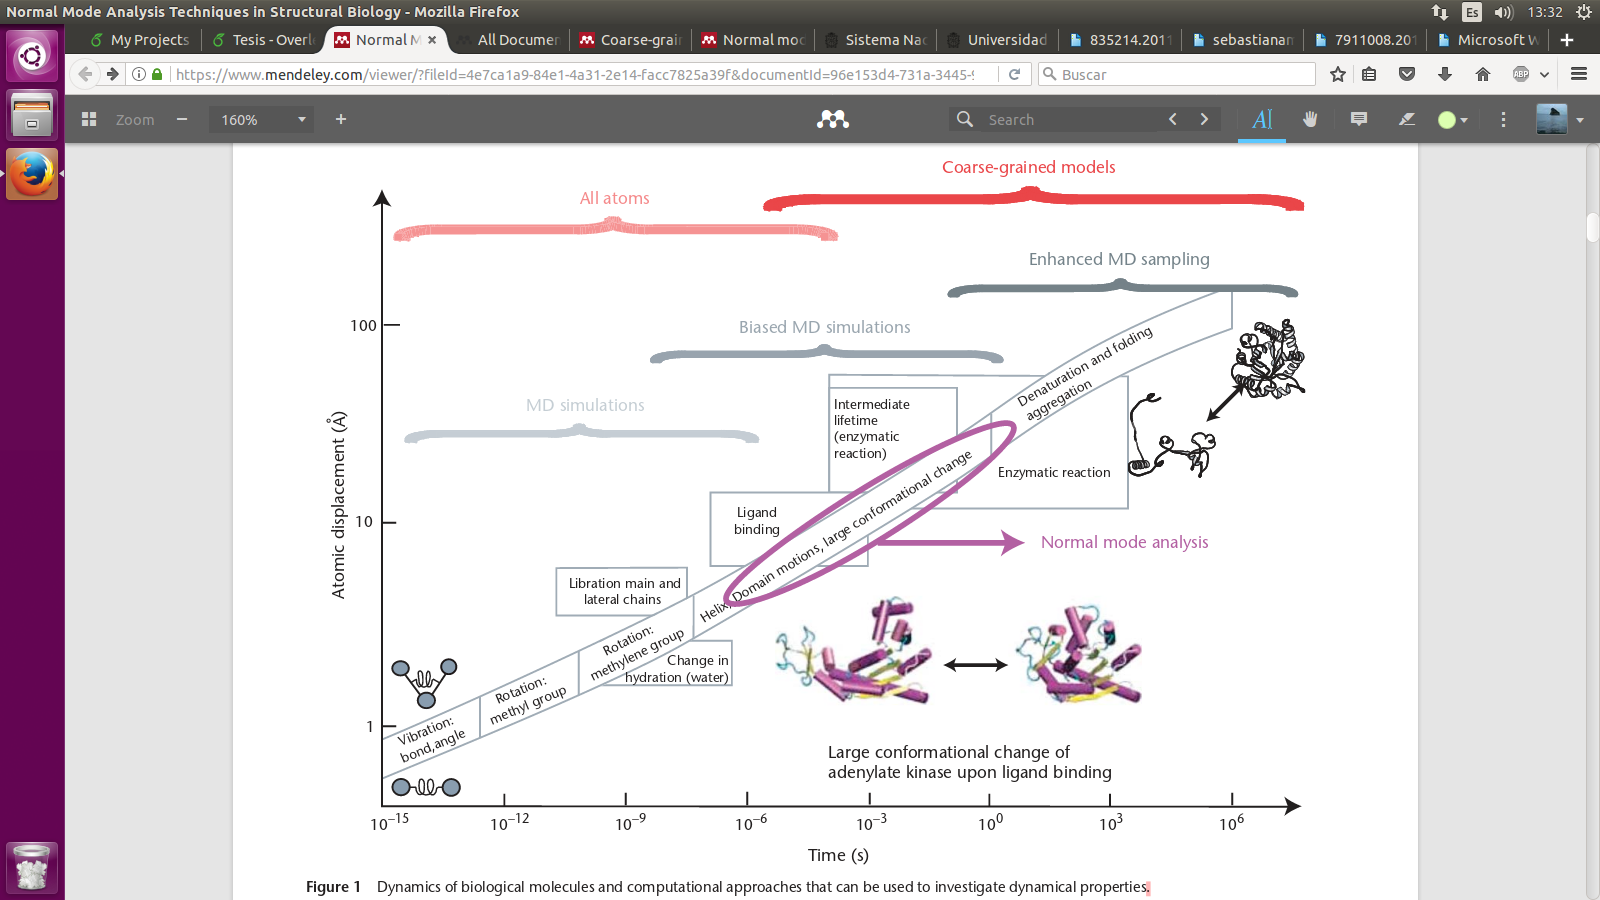
\includegraphics[trim={10cm 1cm 8cm 10cm},clip,scale=0.3]{Kap2/escalas.png}%
\caption{Modelos escogidos de acuerdo a la escala del movimiento y al tiempo de la simulaci\'{o}n computacional.} \label{fig:esc}
\end{figure}



Seg\'{u}n el tipo de modelo a escoger, las soluciones a las ecuaciones de movimiento se encuentran mediante los m\'{e}todos de la din\'{a}mica molecular (Molecular Dynamics que por sus siglas en ingl\'{e}s es MD), el an\'{a}lisis de modos normales (Normal Mode Analysis que por sus siglas en ingl\'{e}s es NMA) o el an\'{a}lisis por componentes principales (Principal Component Analysis, PCA por sus siglas en ingl\'{e}s). Mientras que en MD se obtiene la posici\'{o}n como funci\'{o}n del tiempo, en los NMA y en los PCA  es m\'{a}s importante analizar el espectro, es decir, los autovalores y autovectores obtenidos de una diagonalizaci\'{o}n.\\

\section{Movimientos Locales}
Hacen referencia a las simulaciones en las que se incluyen todos los \'{a}tomos junto con las interacciones presentes, es decir, en las que se analizan los \textit{cambios locales}. Estas se pueden simular a un orden de magnitud de los nanosegundos en una m\'{a}quina usual, al respecto ver \cite{Gur2013}.\\
\subsection{Potenciales Atom\'{i}sticos}
Existen simulaciones MD usando todos los \'{a}tomos (Full atomic MD) o usando los movimientos globales (Coarse-grained models). Como caso particular se pueden considerar los potenciales usados en \cite{Amber2016}, que siguen el modelo de Amber. El modelo de Amber tiene en cuenta las contribuciones debidas a:
 \begin{itemize}
\item Interacciones intermoleculares: Son las producidas por los enlaces covalentes entre grupos de \'{a}tomos, las de valencia y las torsiones.
\begin{eqnarray}
V_{cov}(r)&=&\sum_{enlaces}k_r\left(r-r_0\right)^2\\
V_{val}(r)&=&\sum_{val}k_\theta\left(\theta-\theta_0\right)^2\\
V_{tor}(r)&=&\sum_{torsiones}\sum_{n}\frac{V_n}{2}\left[1+\cos(n\phi-\gamma)\right]
\end{eqnarray}
\item Interacciones entre pares: Lennard Jones, electrost\'{a}tico.
\begin{eqnarray}
V_{len}(r)&=&\sum_{j=1}^{N+1}\sum_{i=j+1}^N f_{ij}\left\{\epsilon_{ij}\left[\left(\frac{r_{0ij}}{r_{ij}}\right)^{12}-2\left(\frac{r_{0ij}}{r_{ij}}\right)^6\right]\right\}\\
V_{elec}(r)&=&\sum_{j=1}^{N-1}\sum_{i=j+1}^{N}\frac{q_iq_j}{4\pi\epsilon_0r_{ij}}
\end{eqnarray}
\end{itemize}
Las constantes $k_r,k_\theta,f_{ij},\epsilon_{ij},r_{0ij},$ son constantes emp\'{i}ricas definidas de manera diferente en cada uno de los programas que realizan din\'{a}mica molecular.\\

Las interacciones consideradas son las mismas que forman y pliegan una prote\'{i}na  en todos sus niveles de estructura, tal como aparece descrito en la secci\'{o}n \ref{ssec:Estruc}. Estas interacciones no forman una estructura tridimensional est\'{a}tica sino din\'{a}mica, es por esto que se resuelven las ecuaciones de movimiento para estos potenciales:
\begin{equation}\label{eq:48}
m_i\frac{\mathrm{d}\mathbf{r_i}}{\mathrm{d}t}=\grad_\mathbf{r_i} V_i
\end{equation}
En este caso $i$ indexa cada \'{a}tomo, $r_i$ su posici\'{o}n y $V_i$ el potencial que se ejerce sobre cada \'{a}tomo.\\

Las simulaciones por MD buscan resolver las ecuaciones de movimiento \eqref{eq:48} de forma num\'{e}rica.\\
\subsection{An\'{a}lisis de Modos Normales Est\'{a}ndar (NMA est\'{a}ndar)}\label{NMAsta}

El an\'{a}lisis de modos normales es el an\'{a}lisis arm\'{o}nico que en este caso es aplicado a las prote\'{i}nas. Los modos normales ocurren cuando todos los constituyentes del sistema oscilan sinusoidalmente y con la misma frecuencia. Los potenciales que cumplen con estas caracter\'{i}sticas son los potenciales tipo Hooke; ya que los potenciales tienen una forma complicada como la del modelo de Amber, entonces se aproxima el potencial alrededor de un punto de equilibrio a una cuadr\'{a}tica.\\

En el an\'{a}lisis \textit{est\'{a}ndar} los constituyentes son \textit{todos los \'{a}tomos} de la biomol\'{e}cula. Al utilizar todos los \'{a}tomos, los costos computacionales de las simulaciones pueden ser mayores que los de otros modelos en los que no se usan todos los \'{a}tomos. A pesar de esto, el NMA est\'{a}ndar es \'{u}til para estudiar los movimientos funcionales de la biomol\'{e}cula.\\

De acuerdo a \cite{Hayward2008}, los pasos requeridos para realizar un modelo de NMA est\'{a}ndar son:
\begin{quote}
 \begin{enumerate}
  \item Una minimizaci\'{o}n de la energ\'{i}a potencial conformacional en funci\'{o}n de las coordenadas cartesianas at\'{o}micas. Se usan las coordenadas at\'{o}micas cristalogr\'{a}ficas.
  \item El c\'{a}lculo de la matriz ``Hessiana", que es la matriz de las segundas derivadas de la energ\'{i}a potencial evaluada en el m\'{i}nimo. 
  \item La diagonalizaci\'{o}n de la matriz de Hessiana.
 \end{enumerate}
\end{quote}


\section{Movimientos Globales}

Son aqu\'{e}llas simulaciones en las que se desean conocer los \textit{cambios globales} o el aspecto general que excibe el movimiento de una biomol\'{e}cula haciendo simplificaciones, ya sea en los potenciales presentes o en el n\'{u}mero de \'{a}tomos interconectados. Algunas de estas simulaciones pueden ser realizadas a un orden de magnitud de los microsegundos y en algotras pueden obtenerse resultados en tan solo unos minutos, lo cual facilita su uso en computadores personales, al respecto ver \cite{Gur2013}. Los modelos en que se reemplaza la descripci\'{o}n atom\'{i}stica por una de m\'{a}s baja resoluci\'{o}n se conocen como modelos de grano grueso, en ingl\'{e}s \textit{coarse-grained models}.\\

De forma semejante a la red cristalina en el estado s\'{o}lido, los bloques constituyentes de la biomol\'{e}cula se reemplazan  por un punto representativo llamdo \textit{nodo}. Aunque los bloques constituyentes son los residuos (mon\'{o}meros) de la biomol\'{e}cula.\\

En una prote\'{i}na las unidades monom\'{e}ricas son los amino\'{a}cidos y  se suelen tomar como nodos las posiciones de equilibrio de los C-$\alpha$ en la estructura cristalina. Ver por ejemplo el tratamiento realizado al inhibidor de la tripsina pancre\'{a}tica bovina (BPTI) y al transportador de aspartato en arqueas GltPh, ver \cite{Gur2013}. Aunque se suelen tomar los C-$\alpha$ esto puede variar ligeramente para dar compatibilidad al modelo con los datos experimentales. Existen programas como MAVEN \cite{Zimmermann2011} que permiten escoger el centro de gravedad de cada mon\'{o}mero como posici\'{o}n de equilibrio del nodo, usar modelos de grano grueso esf\'{e}rico o usar modelos de resoluci\'{o}n mixtals.\\
Un conjunto de modelos que permite calcular los movimientos globales de una mol\'{e}cula son los an\'{a}lisis por modos normales (Normal Mode Analysis o NMA por sus siglas en ingl\'{e}s).
 Otros modelos que describen los movimientos globales son los an\'{a}lisis por componentes principales (Principal Component Analysis o PCA por sus siglas en ingl\'{e}s).
 \subsection{An\'{a}lisis de Modos Normales (NMA)}
Existe una versi\'{o}n equivalente del an\'{a}lisis de modos normales en el cual se usa el mismo potencial pero no se consideran todos los \'{a}tomos de la red sino las unidades monom\'{e}ricas de la biomol\'{e}cula.
\subsubsection{Modelos de Redes El\'{a}sticas (ENM)}
Propuesto por primera vez en \cite{Tirion1996}, los ENM, como la palabra \textit{el\'{a}stico} lo indica, se basan en una simplificaci\'{o}n de la energ\'{i}a potencial a una energ\'{i}a potencial el\'{a}stica, es decir de tipo Hooke, ver figura \ref{fig:pan}.\\



El modelo es bueno cuando la estabilidad de los enlaces con respecto a su posici\'{o}n de equilibrio es menor a una estimaci\'{o}n  de $13\AA$; para distancias mucho mayores el potencial se corta; la distancia a partir de la que se corta el potencial se denomina distancia de corte $R_c$. La distancia de corte es uno de los par\'{a}metros requeridos en el modelo, el otro es la constante el\'{a}stica que puede ser la misma para todas las unidades o puede variar.\\

\begin{figure}
\centering%
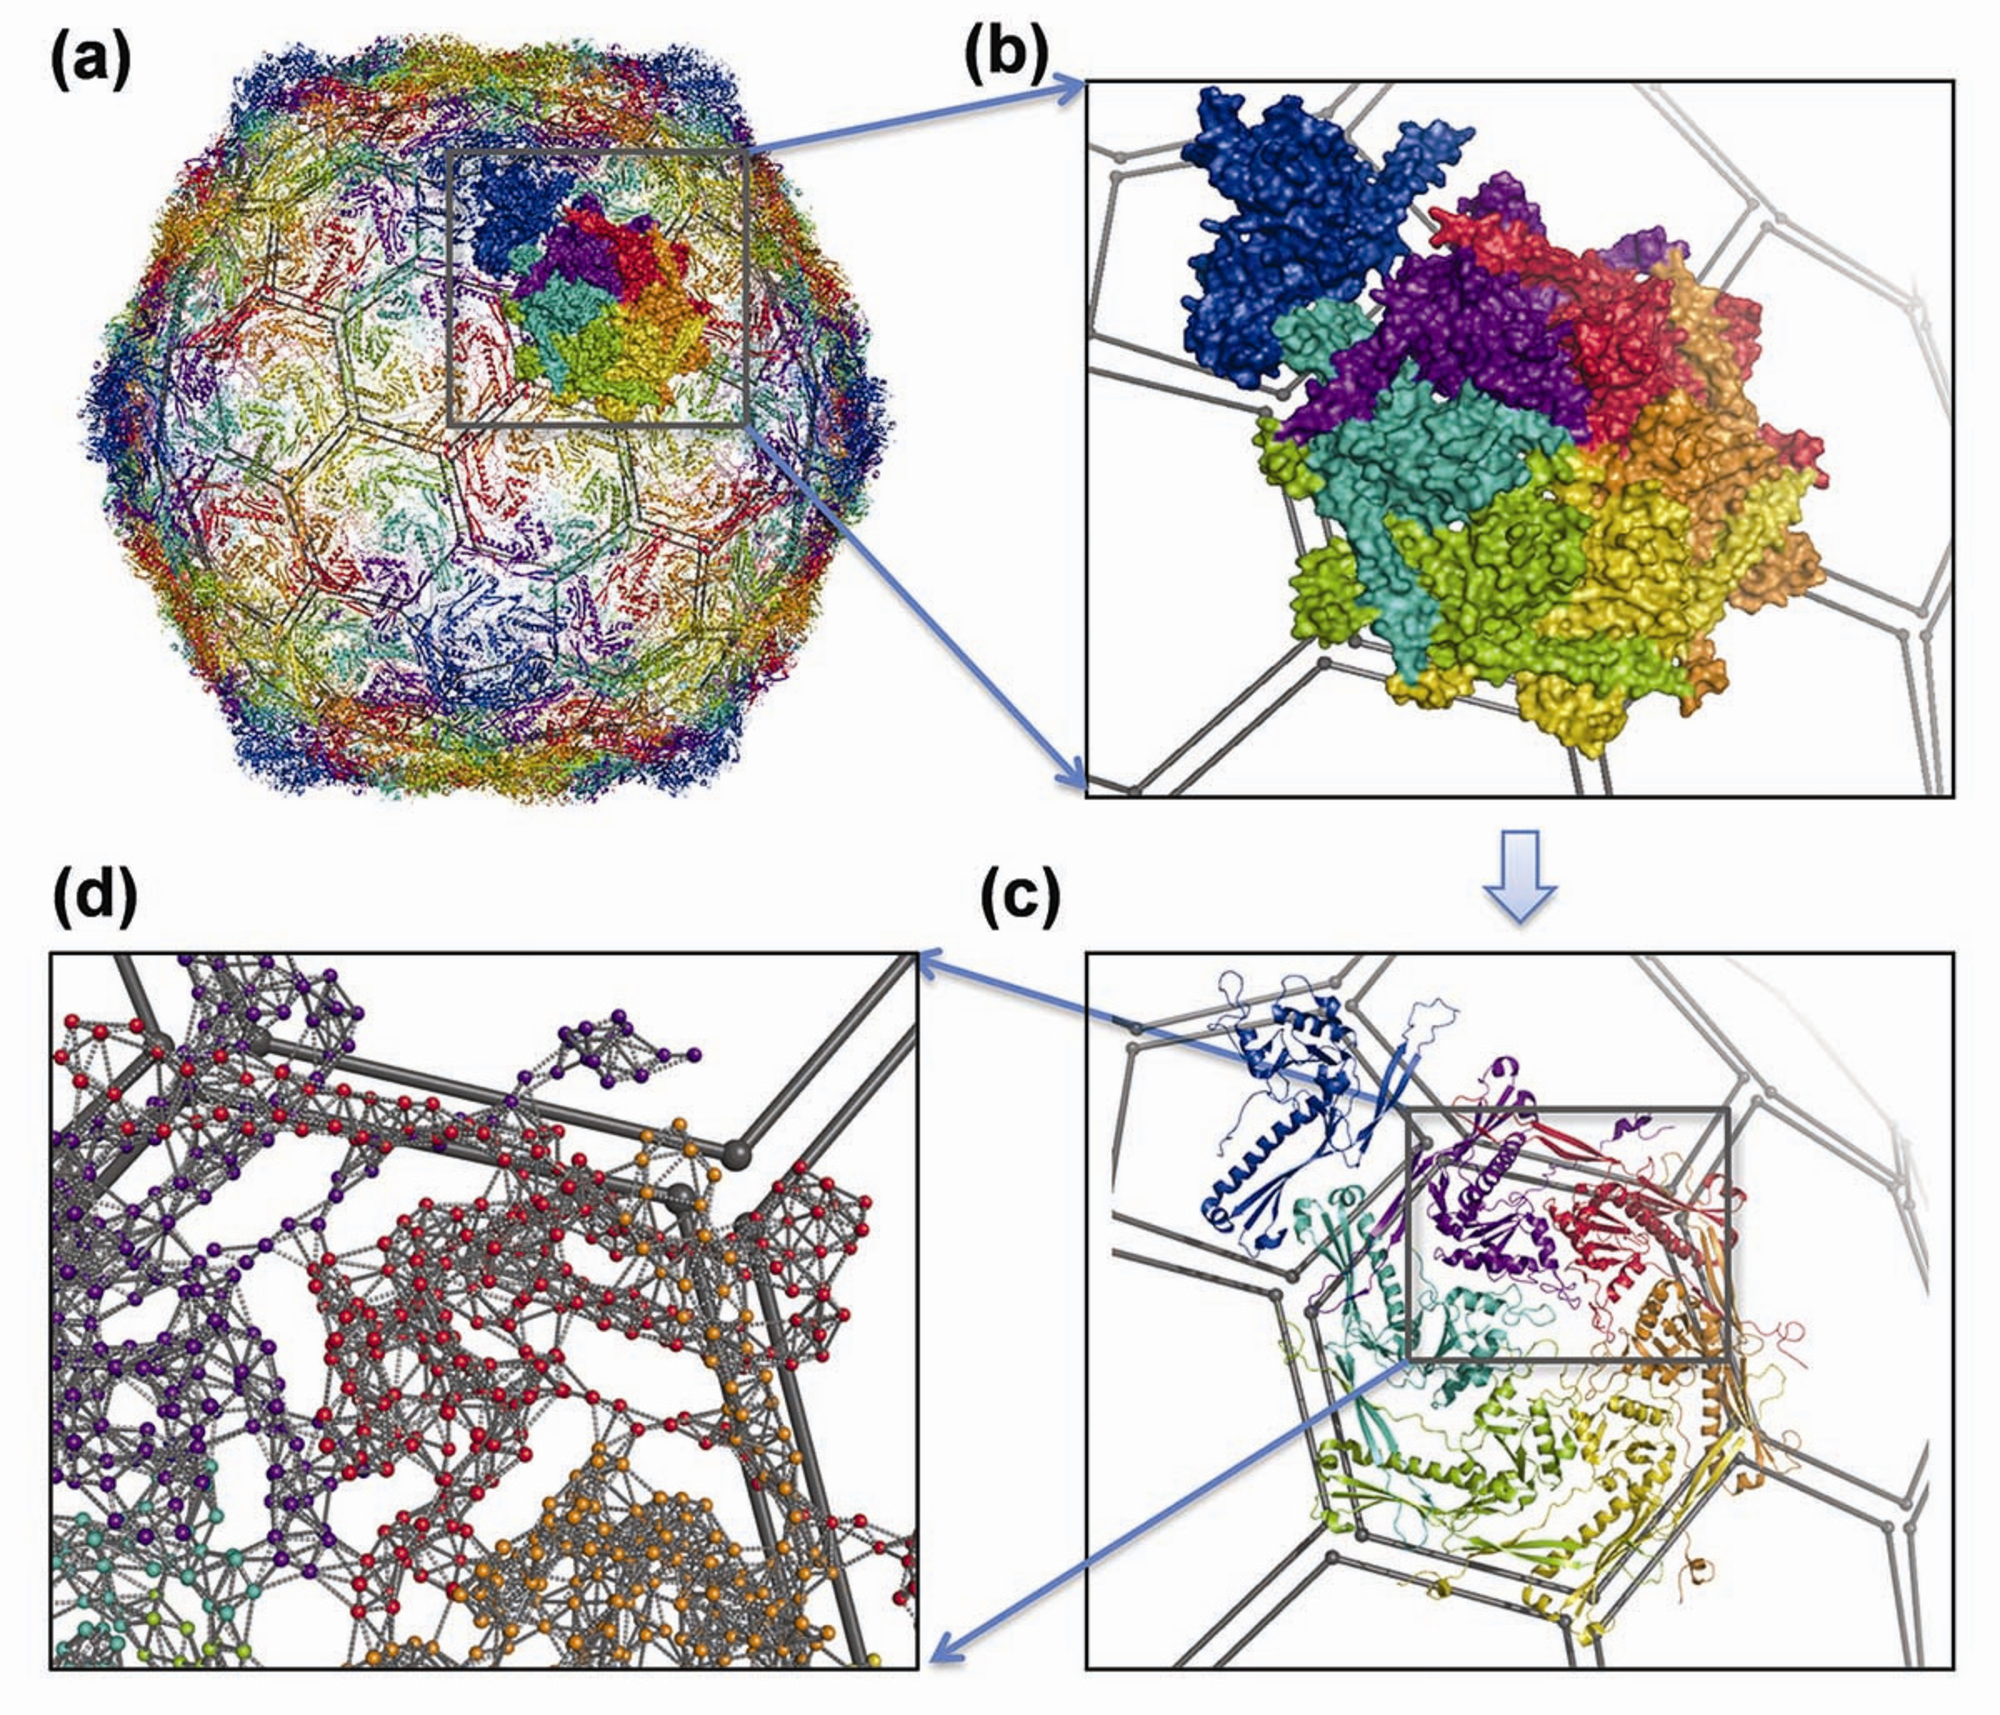
\includegraphics[scale=0.28]{Kap2/dibujo.pdf}%
\caption{ (a) Vista exterior de un c\'{a}pside v\'{i}rico HK97 coloreado por cada cadena, todas las prote\'{i}nas son id\'{e}nticas. (b) Vista del arreglo prote\'{i}nico en una cara del c\'{a}pside. (c) Vista de la estructura secundaria de las prote\'{i}nas (d) Esquema de cada prote\'{i}na mostrando cada uno de sus \'{a}tomos, las aristas de cada cara son carbonos $\alpha$ unidos por lados (ligaduras el\'{a}sticas). Tomado de \cite{Lezon2009}.} \label{fig:pan}
\end{figure}

La primera vez que se usaron los ENM en la investigaci\'{o}n de prote\'{i}nas fue gracias a Monique Tirion, ver \cite{Tirion1996}. Entre las prote\'{i}nas  investigadas se encuentran la actina G (C\'{o}digo PDB: 1atn) y la miosina H1 (C\'{o}digo PDB: 1my). La G-actina es modelada bien por los ENM.\\ 

Existen dos tipos de ENM: Modelos de redes anisotr\'{o}picas (ANM por sus siglas en ingl\'{e}s) y Modelos de Redes Gaussianas (GNM por sus siglas en ingl\'{e}s) los cuales se diferencian en el modelo de potencial usado.  El modelo de redes anisotr\'{o}picas inicialmente no usa el mismo potencial que el an\'{a}lisis de modos normales est\'{a}ndar sino que usa el potencial presente entre resortes tridimensionales, en la figura \ref{fig:ANM} se muestra que el potencial entre los resortes depende de la diferencia de distancias.\\
\begin{figure}
\centering
%LaTeX with PSTricks extensions
%%Creator: inkscape 0.48.5
%%Please note this file requires PSTricks extensions
\psset{xunit=.5pt,yunit=.5pt,runit=.5pt}
\begin{pspicture}(620.04998779,250.19999695)
{
\newrgbcolor{curcolor}{0 0 0}
\pscustom[linewidth=0.96809698,linecolor=curcolor]
{
\newpath
\moveto(240.48010465,176.5854835)
\curveto(240.48010465,166.38227921)(232.62614166,158.11094787)(222.93778733,158.11094787)
\curveto(213.24943299,158.11094787)(205.39547001,166.38227921)(205.39547001,176.5854835)
\curveto(205.39547001,186.78868779)(213.24943299,195.06001913)(222.93778733,195.06001913)
\curveto(232.62614166,195.06001913)(240.48010465,186.78868779)(240.48010465,176.5854835)
\closepath
}
}
{
\newrgbcolor{curcolor}{0 0 0}
\pscustom[linewidth=0.98306393,linecolor=curcolor]
{
\newpath
\moveto(346.60167259,174.05060899)
\curveto(346.60167259,163.85152441)(338.4997138,155.58353276)(328.50544114,155.58353276)
\curveto(318.51116849,155.58353276)(310.4092097,163.85152441)(310.4092097,174.05060899)
\curveto(310.4092097,184.24969356)(318.51116849,192.51768521)(328.50544114,192.51768521)
\curveto(338.4997138,192.51768521)(346.60167259,184.24969356)(346.60167259,174.05060899)
\closepath
}
}
{
\newrgbcolor{curcolor}{0 0 0}
\pscustom[linewidth=0.329673,linecolor=curcolor]
{
\newpath
\moveto(241.4713779,186.50210996)
\curveto(248.58644604,173.65845178)(240.8043424,167.42366304)(240.8043424,167.42366304)
\lineto(240.54394377,167.42366304)
}
}
{
\newrgbcolor{curcolor}{0 0 0}
\pscustom[linewidth=0.329673,linecolor=curcolor]
{
\newpath
\moveto(239.32625885,186.50211345)
\curveto(232.48912399,173.59610791)(240.5491609,167.42366653)(240.5491609,167.42366653)
\lineto(240.80464746,167.42918307)
}
}
{
\newrgbcolor{curcolor}{0 0 0}
\pscustom[linewidth=0.329673,linecolor=curcolor]
{
\newpath
\moveto(243.36542054,186.37741366)
\curveto(250.48048868,173.53375548)(242.69838504,167.29896674)(242.69838504,167.29896674)
\lineto(242.43798641,167.29896674)
}
}
{
\newrgbcolor{curcolor}{0 0 0}
\pscustom[linewidth=0.329673,linecolor=curcolor]
{
\newpath
\moveto(241.49543943,186.50589315)
\curveto(234.65830456,173.59988761)(242.44320353,167.29897023)(242.44320353,167.29897023)
\lineto(242.6986901,167.30448677)
}
}
{
\newrgbcolor{curcolor}{0 0 0}
\pscustom[linewidth=0.329673,linecolor=curcolor]
{
\newpath
\moveto(245.62626995,186.40660762)
\curveto(252.74133809,173.56294944)(244.95923446,167.3281607)(244.95923446,167.3281607)
\lineto(244.69883583,167.3281607)
}
}
{
\newrgbcolor{curcolor}{0 0 0}
\pscustom[linewidth=0.329673,linecolor=curcolor]
{
\newpath
\moveto(243.48115091,186.40661111)
\curveto(236.64401604,173.50060557)(244.70405295,167.32816419)(244.70405295,167.32816419)
\lineto(244.95953951,167.33368073)
}
}
{
\newrgbcolor{curcolor}{0 0 0}
\pscustom[linewidth=0.329673,linecolor=curcolor]
{
\newpath
\moveto(247.52031259,186.28191132)
\curveto(254.63538073,173.43825314)(246.85327709,167.20346439)(246.85327709,167.20346439)
\lineto(246.59287846,167.20346439)
}
}
{
\newrgbcolor{curcolor}{0 0 0}
\pscustom[linewidth=0.329673,linecolor=curcolor]
{
\newpath
\moveto(245.65033148,186.41039081)
\curveto(238.81319662,173.50438527)(246.59809559,167.20346788)(246.59809559,167.20346788)
\lineto(246.85358215,167.20898442)
}
}
{
\newrgbcolor{curcolor}{0 0 0}
\pscustom[linewidth=0.329673,linecolor=curcolor]
{
\newpath
\moveto(249.69439707,186.34047802)
\curveto(256.80946521,173.49681984)(249.02736158,167.2620311)(249.02736158,167.2620311)
\lineto(248.76696295,167.2620311)
}
}
{
\newrgbcolor{curcolor}{0 0 0}
\pscustom[linewidth=0.329673,linecolor=curcolor]
{
\newpath
\moveto(247.54927803,186.34048151)
\curveto(240.71214316,173.43447597)(248.77218007,167.26203459)(248.77218007,167.26203459)
\lineto(249.02766664,167.26755113)
}
}
{
\newrgbcolor{curcolor}{0 0 0}
\pscustom[linewidth=0.329673,linecolor=curcolor]
{
\newpath
\moveto(251.58843971,186.21578172)
\curveto(258.70350785,173.37212354)(250.92140421,167.1373348)(250.92140421,167.1373348)
\lineto(250.66100558,167.1373348)
}
}
{
\newrgbcolor{curcolor}{0 0 0}
\pscustom[linewidth=0.329673,linecolor=curcolor]
{
\newpath
\moveto(249.7184586,186.34426121)
\curveto(242.88132374,173.43825567)(250.66622271,167.13733829)(250.66622271,167.13733829)
\lineto(250.92170927,167.14285483)
}
}
{
\newrgbcolor{curcolor}{0 0 0}
\pscustom[linewidth=0.329673,linecolor=curcolor]
{
\newpath
\moveto(253.89672165,186.23026116)
\curveto(261.01178979,173.38660298)(253.22968615,167.15181423)(253.22968615,167.15181423)
\lineto(252.96928752,167.15181423)
}
}
{
\newrgbcolor{curcolor}{0 0 0}
\pscustom[linewidth=0.329673,linecolor=curcolor]
{
\newpath
\moveto(251.7516026,186.23026465)
\curveto(244.91446773,173.32425911)(252.97450464,167.15181773)(252.97450464,167.15181773)
\lineto(253.22999121,167.15733426)
}
}
{
\newrgbcolor{curcolor}{0 0 0}
\pscustom[linewidth=0.329673,linecolor=curcolor]
{
\newpath
\moveto(255.79076428,186.10556485)
\curveto(262.90583242,173.26190668)(255.12372878,167.02711793)(255.12372878,167.02711793)
\lineto(254.86333015,167.02711793)
}
}
{
\newrgbcolor{curcolor}{0 0 0}
\pscustom[linewidth=0.329673,linecolor=curcolor]
{
\newpath
\moveto(253.92078317,186.23404435)
\curveto(247.08364831,173.3280388)(254.86854728,167.02712142)(254.86854728,167.02712142)
\lineto(255.12403384,167.03263796)
}
}
{
\newrgbcolor{curcolor}{0 0 0}
\pscustom[linewidth=0.329673,linecolor=curcolor]
{
\newpath
\moveto(257.92891504,186.05391497)
\curveto(265.04398318,173.21025679)(257.26187955,166.97546805)(257.26187955,166.97546805)
\lineto(257.00148092,166.97546805)
}
}
{
\newrgbcolor{curcolor}{0 0 0}
\pscustom[linewidth=0.329673,linecolor=curcolor]
{
\newpath
\moveto(255.783796,186.05391846)
\curveto(248.94666113,173.14791292)(257.00669804,166.97547154)(257.00669804,166.97547154)
\lineto(257.26218461,166.98098808)
}
}
{
\newrgbcolor{curcolor}{0 0 0}
\pscustom[linewidth=0.329673,linecolor=curcolor]
{
\newpath
\moveto(259.82295768,185.92921867)
\curveto(266.93802582,173.08556049)(259.15592218,166.85077175)(259.15592218,166.85077175)
\lineto(258.89552355,166.85077175)
}
}
{
\newrgbcolor{curcolor}{0 0 0}
\pscustom[linewidth=0.329673,linecolor=curcolor]
{
\newpath
\moveto(257.95297657,186.05769816)
\curveto(251.11584171,173.15169262)(258.90074068,166.85077524)(258.90074068,166.85077524)
\lineto(259.15622724,166.85629178)
}
}
{
\newrgbcolor{curcolor}{0 0 0}
\pscustom[linewidth=0.329673,linecolor=curcolor]
{
\newpath
\moveto(262.03971955,185.92921923)
\curveto(269.15478769,173.08556105)(261.37268405,166.85077231)(261.37268405,166.85077231)
\lineto(261.11228542,166.85077231)
}
}
{
\newrgbcolor{curcolor}{0 0 0}
\pscustom[linewidth=0.329673,linecolor=curcolor]
{
\newpath
\moveto(259.8946005,185.92922272)
\curveto(253.05746564,173.02321718)(261.11750255,166.8507758)(261.11750255,166.8507758)
\lineto(261.37298911,166.85629234)
}
}
{
\newrgbcolor{curcolor}{0 0 0}
\pscustom[linewidth=0.329673,linecolor=curcolor]
{
\newpath
\moveto(263.93376218,185.80452293)
\curveto(271.04883032,172.96086475)(263.26672669,166.72607601)(263.26672669,166.72607601)
\lineto(263.00632806,166.72607601)
}
}
{
\newrgbcolor{curcolor}{0 0 0}
\pscustom[linewidth=0.329673,linecolor=curcolor]
{
\newpath
\moveto(262.06378108,185.93300242)
\curveto(255.22664621,173.02699688)(263.01154518,166.7260795)(263.01154518,166.7260795)
\lineto(263.26703175,166.73159604)
}
}
{
\newrgbcolor{curcolor}{0 0 0}
\pscustom[linewidth=0.329673,linecolor=curcolor]
{
\newpath
\moveto(266.19987413,185.97693771)
\curveto(273.31494227,173.13327953)(265.53283863,166.89849079)(265.53283863,166.89849079)
\lineto(265.27244,166.89849079)
}
}
{
\newrgbcolor{curcolor}{0 0 0}
\pscustom[linewidth=0.329673,linecolor=curcolor]
{
\newpath
\moveto(264.05475508,185.9769412)
\curveto(257.21762022,173.07093566)(265.27765713,166.89849428)(265.27765713,166.89849428)
\lineto(265.53314369,166.90401082)
}
}
{
\newrgbcolor{curcolor}{0 0 0}
\pscustom[linewidth=0.329673,linecolor=curcolor]
{
\newpath
\moveto(268.09391676,185.85224141)
\curveto(275.2089849,173.00858323)(267.42688127,166.77379449)(267.42688127,166.77379449)
\lineto(267.16648264,166.77379449)
}
}
{
\newrgbcolor{curcolor}{0 0 0}
\pscustom[linewidth=0.329673,linecolor=curcolor]
{
\newpath
\moveto(266.22393566,185.9807209)
\curveto(259.38680079,173.07471536)(267.17169976,166.77379798)(267.17169976,166.77379798)
\lineto(267.42718633,166.77931452)
}
}
{
\newrgbcolor{curcolor}{0 0 0}
\pscustom[linewidth=0.329673,linecolor=curcolor]
{
\newpath
\moveto(270.24783968,185.87756833)
\curveto(277.36290782,173.03391015)(269.58080418,166.79912141)(269.58080418,166.79912141)
\lineto(269.32040555,166.79912141)
}
}
{
\newrgbcolor{curcolor}{0 0 0}
\pscustom[linewidth=0.329673,linecolor=curcolor]
{
\newpath
\moveto(268.10272063,185.87757182)
\curveto(261.26558576,172.97156628)(269.32562268,166.7991249)(269.32562268,166.7991249)
\lineto(269.58110924,166.80464144)
}
}
{
\newrgbcolor{curcolor}{0 0 0}
\pscustom[linewidth=0.329673,linecolor=curcolor]
{
\newpath
\moveto(272.14188231,185.75287203)
\curveto(279.25695045,172.90921385)(271.47484682,166.67442511)(271.47484682,166.67442511)
\lineto(271.21444819,166.67442511)
}
}
{
\newrgbcolor{curcolor}{0 0 0}
\pscustom[linewidth=0.329673,linecolor=curcolor]
{
\newpath
\moveto(270.27190121,185.88135152)
\curveto(263.43476634,172.97534598)(271.21966531,166.6744286)(271.21966531,166.6744286)
\lineto(271.47515188,166.67994514)
}
}
{
\newrgbcolor{curcolor}{0 0 0}
\pscustom[linewidth=0.329673,linecolor=curcolor]
{
\newpath
\moveto(274.36817913,185.88826567)
\curveto(281.48324727,173.04460749)(273.70114364,166.80981875)(273.70114364,166.80981875)
\lineto(273.440745,166.80981875)
}
}
{
\newrgbcolor{curcolor}{0 0 0}
\pscustom[linewidth=0.329673,linecolor=curcolor]
{
\newpath
\moveto(272.22306008,185.88826916)
\curveto(265.38592522,172.98226362)(273.44596213,166.80982224)(273.44596213,166.80982224)
\lineto(273.70144869,166.81533878)
}
}
{
\newrgbcolor{curcolor}{0 0 0}
\pscustom[linewidth=0.329673,linecolor=curcolor]
{
\newpath
\moveto(276.26222177,185.76356937)
\curveto(283.37728991,172.91991119)(275.59518627,166.68512244)(275.59518627,166.68512244)
\lineto(275.33478764,166.68512244)
}
}
{
\newrgbcolor{curcolor}{0 0 0}
\pscustom[linewidth=0.329673,linecolor=curcolor]
{
\newpath
\moveto(274.39224066,185.89204886)
\curveto(267.55510579,172.98604332)(275.34000476,166.68512593)(275.34000476,166.68512593)
\lineto(275.59549133,166.69064247)
}
}
{
\newrgbcolor{curcolor}{0 0 0}
\pscustom[linewidth=0.329673,linecolor=curcolor]
{
\newpath
\moveto(278.46665678,185.65370495)
\curveto(285.58172492,172.81004677)(277.79962128,166.57525803)(277.79962128,166.57525803)
\lineto(277.53922265,166.57525803)
}
}
{
\newrgbcolor{curcolor}{0 0 0}
\pscustom[linewidth=0.329673,linecolor=curcolor]
{
\newpath
\moveto(276.32153773,185.65370844)
\curveto(269.48440287,172.7477029)(277.54443978,166.57526152)(277.54443978,166.57526152)
\lineto(277.79992634,166.58077806)
}
}
{
\newrgbcolor{curcolor}{0 0 0}
\pscustom[linewidth=0.329673,linecolor=curcolor]
{
\newpath
\moveto(280.36069942,185.52900865)
\curveto(287.47576756,172.68535047)(279.69366392,166.45056172)(279.69366392,166.45056172)
\lineto(279.43326529,166.45056172)
}
}
{
\newrgbcolor{curcolor}{0 0 0}
\pscustom[linewidth=0.329673,linecolor=curcolor]
{
\newpath
\moveto(278.49071831,185.65748814)
\curveto(271.65358344,172.7514826)(279.43848241,166.45056522)(279.43848241,166.45056522)
\lineto(279.69396898,166.45608175)
}
}
{
\newrgbcolor{curcolor}{0 0 0}
\pscustom[linewidth=0.329673,linecolor=curcolor]
{
\newpath
\moveto(282.62155159,185.55820249)
\curveto(289.73661973,172.71454431)(281.95451609,166.47975557)(281.95451609,166.47975557)
\lineto(281.69411746,166.47975557)
}
}
{
\newrgbcolor{curcolor}{0 0 0}
\pscustom[linewidth=0.329673,linecolor=curcolor]
{
\newpath
\moveto(280.47643254,185.55820598)
\curveto(273.63929768,172.65220044)(281.69933459,166.47975906)(281.69933459,166.47975906)
\lineto(281.95482115,166.4852756)
}
}
{
\newrgbcolor{curcolor}{0 0 0}
\pscustom[linewidth=0.329673,linecolor=curcolor]
{
\newpath
\moveto(284.51559423,185.43350619)
\curveto(291.63066237,172.58984801)(283.84855873,166.35505926)(283.84855873,166.35505926)
\lineto(283.5881601,166.35505926)
}
}
{
\newrgbcolor{curcolor}{0 0 0}
\pscustom[linewidth=0.329673,linecolor=curcolor]
{
\newpath
\moveto(282.64561312,185.56198568)
\curveto(275.80847825,172.65598014)(283.59337722,166.35506276)(283.59337722,166.35506276)
\lineto(283.84886379,166.36057929)
}
}
{
\newrgbcolor{curcolor}{0 0 0}
\pscustom[linewidth=0.329673,linecolor=curcolor]
{
\newpath
\moveto(286.68967591,185.49207385)
\curveto(293.80474405,172.64841567)(286.02264041,166.41362693)(286.02264041,166.41362693)
\lineto(285.76224178,166.41362693)
}
}
{
\newrgbcolor{curcolor}{0 0 0}
\pscustom[linewidth=0.329673,linecolor=curcolor]
{
\newpath
\moveto(284.54455686,185.49207734)
\curveto(277.707422,172.5860718)(285.76745891,166.41363042)(285.76745891,166.41363042)
\lineto(286.02294547,166.41914696)
}
}
{
\newrgbcolor{curcolor}{0 0 0}
\pscustom[linewidth=0.329673,linecolor=curcolor]
{
\newpath
\moveto(288.58371855,185.36737755)
\curveto(295.69878668,172.52371937)(287.91668305,166.28893063)(287.91668305,166.28893063)
\lineto(287.65628442,166.28893063)
}
}
{
\newrgbcolor{curcolor}{0 0 0}
\pscustom[linewidth=0.329673,linecolor=curcolor]
{
\newpath
\moveto(286.71373744,185.49585704)
\curveto(279.87660257,172.5898515)(287.66150154,166.28893412)(287.66150154,166.28893412)
\lineto(287.91698811,166.29445066)
}
}
{
\newrgbcolor{curcolor}{0 0 0}
\pscustom[linewidth=0.329673,linecolor=curcolor]
{
\newpath
\moveto(290.8920011,185.38185829)
\curveto(298.00706924,172.53820011)(290.22496561,166.30341137)(290.22496561,166.30341137)
\lineto(289.96456698,166.30341137)
}
}
{
\newrgbcolor{curcolor}{0 0 0}
\pscustom[linewidth=0.329673,linecolor=curcolor]
{
\newpath
\moveto(288.74688206,185.38186178)
\curveto(281.90974719,172.47585624)(289.9697841,166.30341486)(289.9697841,166.30341486)
\lineto(290.22527066,166.3089314)
}
}
{
\newrgbcolor{curcolor}{0 0 0}
\pscustom[linewidth=0.329673,linecolor=curcolor]
{
\newpath
\moveto(292.78604374,185.25716199)
\curveto(299.90111188,172.41350381)(292.11900824,166.17871507)(292.11900824,166.17871507)
\lineto(291.85860961,166.17871507)
}
}
{
\newrgbcolor{curcolor}{0 0 0}
\pscustom[linewidth=0.329673,linecolor=curcolor]
{
\newpath
\moveto(290.91606263,185.38564148)
\curveto(284.07892776,172.47963594)(291.86382673,166.17871856)(291.86382673,166.17871856)
\lineto(292.1193133,166.1842351)
}
}
{
\newrgbcolor{curcolor}{0 0 0}
\pscustom[linewidth=0.329673,linecolor=curcolor]
{
\newpath
\moveto(294.92419388,185.20551061)
\curveto(302.03926202,172.36185243)(294.25715838,166.12706368)(294.25715838,166.12706368)
\lineto(293.99675975,166.12706368)
}
}
{
\newrgbcolor{curcolor}{0 0 0}
\pscustom[linewidth=0.329673,linecolor=curcolor]
{
\newpath
\moveto(292.77907483,185.2055141)
\curveto(285.94193997,172.29950855)(294.00197688,166.12706717)(294.00197688,166.12706717)
\lineto(294.25746344,166.13258371)
}
}
{
\newrgbcolor{curcolor}{0 0 0}
\pscustom[linewidth=0.329673,linecolor=curcolor]
{
\newpath
\moveto(296.81823651,185.0808143)
\curveto(303.93330465,172.23715613)(296.15120102,166.00236738)(296.15120102,166.00236738)
\lineto(295.89080239,166.00236738)
}
}
{
\newrgbcolor{curcolor}{0 0 0}
\pscustom[linewidth=0.329673,linecolor=curcolor]
{
\newpath
\moveto(294.94825541,185.2092938)
\curveto(288.11112054,172.30328825)(295.89601951,166.00237087)(295.89601951,166.00237087)
\lineto(296.15150608,166.00788741)
}
}
{
\newrgbcolor{curcolor}{0 0 0}
\pscustom[linewidth=0.329673,linecolor=curcolor]
{
\newpath
\moveto(299.03499839,185.08081588)
\curveto(306.15006652,172.2371577)(298.36796289,166.00236896)(298.36796289,166.00236896)
\lineto(298.10756426,166.00236896)
}
}
{
\newrgbcolor{curcolor}{0 0 0}
\pscustom[linewidth=0.329673,linecolor=curcolor]
{
\newpath
\moveto(296.88987934,185.08081937)
\curveto(290.05274447,172.17481383)(298.11278138,166.00237245)(298.11278138,166.00237245)
\lineto(298.36826795,166.00788899)
}
}
{
\newrgbcolor{curcolor}{0 0 0}
\pscustom[linewidth=0.329673,linecolor=curcolor]
{
\newpath
\moveto(300.92904102,184.95611958)
\curveto(308.04410916,172.1124614)(300.26200552,165.87767265)(300.26200552,165.87767265)
\lineto(300.00160689,165.87767265)
}
}
{
\newrgbcolor{curcolor}{0 0 0}
\pscustom[linewidth=0.329673,linecolor=curcolor]
{
\newpath
\moveto(299.05905991,185.08459907)
\curveto(292.22192505,172.17859353)(300.00682402,165.87767615)(300.00682402,165.87767615)
\lineto(300.26231058,165.88319268)
}
}
{
\newrgbcolor{curcolor}{0 0 0}
\pscustom[linewidth=0.329673,linecolor=curcolor]
{
\newpath
\moveto(303.1951539,185.12853394)
\curveto(310.31022204,172.28487576)(302.5281184,166.05008702)(302.5281184,166.05008702)
\lineto(302.26771977,166.05008702)
}
}
{
\newrgbcolor{curcolor}{0 0 0}
\pscustom[linewidth=0.329673,linecolor=curcolor]
{
\newpath
\moveto(301.05003485,185.12853743)
\curveto(294.21289998,172.22253189)(302.27293689,166.05009051)(302.27293689,166.05009051)
\lineto(302.52842346,166.05560705)
}
}
{
\newrgbcolor{curcolor}{0 0 0}
\pscustom[linewidth=0.329673,linecolor=curcolor]
{
\newpath
\moveto(305.08919653,185.00383764)
\curveto(312.20426467,172.16017946)(304.42216104,165.92539071)(304.42216104,165.92539071)
\lineto(304.16176241,165.92539071)
}
}
{
\newrgbcolor{curcolor}{0 0 0}
\pscustom[linewidth=0.329673,linecolor=curcolor]
{
\newpath
\moveto(303.21921543,185.13231713)
\curveto(296.38208056,172.22631159)(304.16697953,165.92539421)(304.16697953,165.92539421)
\lineto(304.42246609,165.93091075)
}
}
{
\newrgbcolor{curcolor}{0 0 0}
\pscustom[linewidth=0.329673,linecolor=curcolor]
{
\newpath
\moveto(307.24311945,185.02916641)
\curveto(314.35818759,172.18550823)(306.57608395,165.95071949)(306.57608395,165.95071949)
\lineto(306.31568532,165.95071949)
}
}
{
\newrgbcolor{curcolor}{0 0 0}
\pscustom[linewidth=0.329673,linecolor=curcolor]
{
\newpath
\moveto(305.0980004,185.0291699)
\curveto(298.26086553,172.12316436)(306.32090244,165.95072298)(306.32090244,165.95072298)
\lineto(306.57638901,165.95623952)
}
}
{
\newrgbcolor{curcolor}{0 0 0}
\pscustom[linewidth=0.329673,linecolor=curcolor]
{
\newpath
\moveto(309.13716208,184.90447011)
\curveto(316.25223022,172.06081193)(308.47012659,165.82602319)(308.47012659,165.82602319)
\lineto(308.20972796,165.82602319)
}
}
{
\newrgbcolor{curcolor}{0 0 0}
\pscustom[linewidth=0.329673,linecolor=curcolor]
{
\newpath
\moveto(307.26718098,185.0329496)
\curveto(300.43004611,172.12694406)(308.21494508,165.82602668)(308.21494508,165.82602668)
\lineto(308.47043164,165.83154322)
}
}
{
\newrgbcolor{curcolor}{0 0 0}
\pscustom[linewidth=0.329673,linecolor=curcolor]
{
\newpath
\moveto(311.36345859,185.03986081)
\curveto(318.47852673,172.19620264)(310.69642309,165.96141389)(310.69642309,165.96141389)
\lineto(310.43602446,165.96141389)
}
}
{
\newrgbcolor{curcolor}{0 0 0}
\pscustom[linewidth=0.329673,linecolor=curcolor]
{
\newpath
\moveto(309.21833954,185.03986431)
\curveto(302.38120468,172.13385876)(310.44124159,165.96141738)(310.44124159,165.96141738)
\lineto(310.69672815,165.96693392)
}
}
{
\newrgbcolor{curcolor}{0 0 0}
\pscustom[linewidth=0.329673,linecolor=curcolor]
{
\newpath
\moveto(313.25750123,184.91516451)
\curveto(320.37256937,172.07150633)(312.59046573,165.83671759)(312.59046573,165.83671759)
\lineto(312.3300671,165.83671759)
}
}
{
\newrgbcolor{curcolor}{0 0 0}
\pscustom[linewidth=0.329673,linecolor=curcolor]
{
\newpath
\moveto(311.38752012,185.043644)
\curveto(304.55038525,172.13763846)(312.33528422,165.83672108)(312.33528422,165.83672108)
\lineto(312.59077079,165.84223762)
}
}
{
\newrgbcolor{curcolor}{0 0 0}
\pscustom[linewidth=0.99451757,linecolor=curcolor]
{
\newpath
\moveto(249.49099243,128.11175157)
\curveto(246.84433855,118.57485364)(236.27413795,112.43969329)(225.88178859,114.40848739)
\curveto(215.48943924,116.3772815)(209.2103124,125.70448778)(211.85696628,135.24138572)
\curveto(214.50362016,144.77828365)(225.07382076,150.913444)(235.46617012,148.9446499)
\curveto(245.85851947,146.97585579)(252.1376463,137.64864951)(249.49099243,128.11175157)
\closepath
}
}
{
\newrgbcolor{curcolor}{0 0 0}
\pscustom[linewidth=0.95157243,linecolor=curcolor]
{
\newpath
\moveto(367.33185651,105.90041566)
\curveto(364.91177965,96.3519429)(355.24648188,90.20933606)(345.74380973,92.18051929)
\curveto(336.24113758,94.15170252)(330.49955967,103.49022883)(332.91963653,113.0387016)
\curveto(335.3397134,122.58717436)(345.00501117,128.7297812)(354.50768332,126.75859797)
\curveto(364.01035547,124.78741474)(369.75193338,115.44888843)(367.33185651,105.90041566)
\closepath
}
}
{
\newrgbcolor{curcolor}{0 0 0}
\pscustom[linewidth=0.35938292,linecolor=curcolor]
{
\newpath
\moveto(251.41734966,138.64167701)
\curveto(256.44401602,124.82965504)(245.55472408,120.63382247)(245.55472408,120.63382247)
\lineto(245.24581018,120.69197024)
}
}
{
\newrgbcolor{curcolor}{0 0 0}
\pscustom[linewidth=0.35938292,linecolor=curcolor]
{
\newpath
\moveto(248.87257112,139.12069157)
\curveto(237.33100533,128.36490105)(245.25200025,120.69080856)(245.25200025,120.69080856)
\lineto(245.55655328,120.63900772)
}
}
{
\newrgbcolor{curcolor}{0 0 0}
\pscustom[linewidth=0.35938292,linecolor=curcolor]
{
\newpath
\moveto(253.63112829,138.10005938)
\curveto(258.65779465,124.28803742)(247.76850271,120.09220485)(247.76850271,120.09220485)
\lineto(247.45958881,120.15035261)
}
}
{
\newrgbcolor{curcolor}{0 0 0}
\pscustom[linewidth=0.35938292,linecolor=curcolor]
{
\newpath
\moveto(251.44689975,138.63990443)
\curveto(239.90533396,127.88411391)(247.46577888,120.14919093)(247.46577888,120.14919093)
\lineto(247.77033191,120.0973901)
}
}
{
\newrgbcolor{curcolor}{0 0 0}
\pscustom[linewidth=0.35938292,linecolor=curcolor]
{
\newpath
\moveto(256.32096019,137.62298888)
\curveto(261.34762654,123.81096692)(250.45833461,119.61513435)(250.45833461,119.61513435)
\lineto(250.14942071,119.67328211)
}
}
{
\newrgbcolor{curcolor}{0 0 0}
\pscustom[linewidth=0.35938292,linecolor=curcolor]
{
\newpath
\moveto(253.77618165,138.10200344)
\curveto(242.23461586,127.34621292)(250.15561077,119.67212043)(250.15561077,119.67212043)
\lineto(250.4601638,119.6203196)
}
}
{
\newrgbcolor{curcolor}{0 0 0}
\pscustom[linewidth=0.35938292,linecolor=curcolor]
{
\newpath
\moveto(258.53473882,137.08137126)
\curveto(263.56140518,123.26934929)(252.67211324,119.07351672)(252.67211324,119.07351672)
\lineto(252.36319934,119.13166448)
}
}
{
\newrgbcolor{curcolor}{0 0 0}
\pscustom[linewidth=0.35938292,linecolor=curcolor]
{
\newpath
\moveto(256.35051028,137.62121631)
\curveto(244.80894449,126.86542579)(252.36938941,119.13050281)(252.36938941,119.13050281)
\lineto(252.67394244,119.07870197)
}
}
{
\newrgbcolor{curcolor}{0 0 0}
\pscustom[linewidth=0.35938292,linecolor=curcolor]
{
\newpath
\moveto(261.12944816,136.65162942)
\curveto(266.15611451,122.83960746)(255.26682258,118.64377489)(255.26682258,118.64377489)
\lineto(254.95790868,118.70192265)
}
}
{
\newrgbcolor{curcolor}{0 0 0}
\pscustom[linewidth=0.35938292,linecolor=curcolor]
{
\newpath
\moveto(258.58466962,137.13064398)
\curveto(247.04310383,126.37485346)(254.96409874,118.70076097)(254.96409874,118.70076097)
\lineto(255.26865177,118.64896014)
}
}
{
\newrgbcolor{curcolor}{0 0 0}
\pscustom[linewidth=0.35938292,linecolor=curcolor]
{
\newpath
\moveto(263.34322679,136.1100118)
\curveto(268.36989315,122.29798983)(257.48060121,118.10215726)(257.48060121,118.10215726)
\lineto(257.17168731,118.16030502)
}
}
{
\newrgbcolor{curcolor}{0 0 0}
\pscustom[linewidth=0.35938292,linecolor=curcolor]
{
\newpath
\moveto(261.15899825,136.64985685)
\curveto(249.61743246,125.89406633)(257.17787738,118.15914335)(257.17787738,118.15914335)
\lineto(257.48243041,118.10734251)
}
}
{
\newrgbcolor{curcolor}{0 0 0}
\pscustom[linewidth=0.35938292,linecolor=curcolor]
{
\newpath
\moveto(266.08541711,135.60834579)
\curveto(271.11208346,121.79632382)(260.22279153,117.60049125)(260.22279153,117.60049125)
\lineto(259.91387763,117.65863901)
}
}
{
\newrgbcolor{curcolor}{0 0 0}
\pscustom[linewidth=0.35938292,linecolor=curcolor]
{
\newpath
\moveto(263.54063857,136.08736035)
\curveto(251.99907278,125.33156983)(259.92006769,117.65747734)(259.92006769,117.65747734)
\lineto(260.22462073,117.6056765)
}
}
{
\newrgbcolor{curcolor}{0 0 0}
\pscustom[linewidth=0.35938292,linecolor=curcolor]
{
\newpath
\moveto(268.29919574,135.06672816)
\curveto(273.3258621,121.2547062)(262.43657016,117.05887363)(262.43657016,117.05887363)
\lineto(262.12765626,117.11702139)
}
}
{
\newrgbcolor{curcolor}{0 0 0}
\pscustom[linewidth=0.35938292,linecolor=curcolor]
{
\newpath
\moveto(266.1149672,135.60657321)
\curveto(254.57340141,124.85078269)(262.13384633,117.11585971)(262.13384633,117.11585971)
\lineto(262.43839936,117.06405888)
}
}
{
\newrgbcolor{curcolor}{0 0 0}
\pscustom[linewidth=0.35938292,linecolor=curcolor]
{
\newpath
\moveto(270.82197941,134.54011819)
\curveto(275.84864576,120.72809622)(264.95935383,116.53226365)(264.95935383,116.53226365)
\lineto(264.65043993,116.59041141)
}
}
{
\newrgbcolor{curcolor}{0 0 0}
\pscustom[linewidth=0.35938292,linecolor=curcolor]
{
\newpath
\moveto(268.27720086,135.01913274)
\curveto(256.73563508,124.26334222)(264.65662999,116.58924974)(264.65662999,116.58924974)
\lineto(264.96118302,116.5374489)
}
}
{
\newrgbcolor{curcolor}{0 0 0}
\pscustom[linewidth=0.35938292,linecolor=curcolor]
{
\newpath
\moveto(273.03575804,133.99850056)
\curveto(278.06242439,120.18647859)(267.17313246,115.99064603)(267.17313246,115.99064603)
\lineto(266.86421856,116.04879379)
}
}
{
\newrgbcolor{curcolor}{0 0 0}
\pscustom[linewidth=0.35938292,linecolor=curcolor]
{
\newpath
\moveto(270.8515295,134.53834561)
\curveto(259.30996371,123.78255509)(266.87040862,116.04763211)(266.87040862,116.04763211)
\lineto(267.17496165,115.99583127)
}
}
{
\newrgbcolor{curcolor}{0 0 0}
\pscustom[linewidth=0.35938292,linecolor=curcolor]
{
\newpath
\moveto(275.66552836,133.50349181)
\curveto(280.69219472,119.69146985)(269.80290278,115.49563728)(269.80290278,115.49563728)
\lineto(269.49398888,115.55378504)
}
}
{
\newrgbcolor{curcolor}{0 0 0}
\pscustom[linewidth=0.35938292,linecolor=curcolor]
{
\newpath
\moveto(273.12074982,133.98250637)
\curveto(261.57918403,123.22671585)(269.50017895,115.55262336)(269.50017895,115.55262336)
\lineto(269.80473198,115.50082253)
}
}
{
\newrgbcolor{curcolor}{0 0 0}
\pscustom[linewidth=0.35938292,linecolor=curcolor]
{
\newpath
\moveto(277.879307,132.96187419)
\curveto(282.90597335,119.14985222)(272.01668142,114.95401965)(272.01668142,114.95401965)
\lineto(271.70776752,115.01216742)
}
}
{
\newrgbcolor{curcolor}{0 0 0}
\pscustom[linewidth=0.35938292,linecolor=curcolor]
{
\newpath
\moveto(275.69507846,133.50171924)
\curveto(264.15351267,122.74592872)(271.71395758,115.01100574)(271.71395758,115.01100574)
\lineto(272.01851061,114.9592049)
}
}
{
\newrgbcolor{curcolor}{0 0 0}
\pscustom[linewidth=0.35938292,linecolor=curcolor]
{
\newpath
\moveto(280.61345196,132.61993067)
\curveto(285.64011831,118.8079087)(274.75082638,114.61207613)(274.75082638,114.61207613)
\lineto(274.44191248,114.67022389)
}
}
{
\newrgbcolor{curcolor}{0 0 0}
\pscustom[linewidth=0.35938292,linecolor=curcolor]
{
\newpath
\moveto(278.06867341,133.09894522)
\curveto(266.52710762,122.3431547)(274.44810254,114.66906222)(274.44810254,114.66906222)
\lineto(274.75265557,114.61726138)
}
}
{
\newrgbcolor{curcolor}{0 0 0}
\pscustom[linewidth=0.35938292,linecolor=curcolor]
{
\newpath
\moveto(282.82723059,132.07831304)
\curveto(287.85389694,118.26629107)(276.96460501,114.07045851)(276.96460501,114.07045851)
\lineto(276.65569111,114.12860627)
}
}
{
\newrgbcolor{curcolor}{0 0 0}
\pscustom[linewidth=0.35938292,linecolor=curcolor]
{
\newpath
\moveto(280.64300205,132.61815809)
\curveto(269.10143626,121.86236757)(276.66188117,114.12744459)(276.66188117,114.12744459)
\lineto(276.9664342,114.07564375)
}
}
{
\newrgbcolor{curcolor}{0 0 0}
\pscustom[linewidth=0.35938292,linecolor=curcolor]
{
\newpath
\moveto(285.38918643,131.62143931)
\curveto(290.41585278,117.80941734)(279.52656085,113.61358477)(279.52656085,113.61358477)
\lineto(279.21764695,113.67173253)
}
}
{
\newrgbcolor{curcolor}{0 0 0}
\pscustom[linewidth=0.35938292,linecolor=curcolor]
{
\newpath
\moveto(282.84440789,132.10045386)
\curveto(271.3028421,121.34466334)(279.22383701,113.67057086)(279.22383701,113.67057086)
\lineto(279.52839004,113.61877002)
}
}
{
\newrgbcolor{curcolor}{0 0 0}
\pscustom[linewidth=0.35938292,linecolor=curcolor]
{
\newpath
\moveto(287.60296506,131.07982168)
\curveto(292.62963142,117.26779972)(281.74033948,113.07196715)(281.74033948,113.07196715)
\lineto(281.43142558,113.13011491)
}
}
{
\newrgbcolor{curcolor}{0 0 0}
\pscustom[linewidth=0.35938292,linecolor=curcolor]
{
\newpath
\moveto(285.41873652,131.61966673)
\curveto(273.87717073,120.86387621)(281.43761565,113.12895323)(281.43761565,113.12895323)
\lineto(281.74216868,113.0771524)
}
}
{
\newrgbcolor{curcolor}{0 0 0}
\pscustom[linewidth=0.35938292,linecolor=curcolor]
{
\newpath
\moveto(290.28003615,130.71153626)
\curveto(295.3067025,116.8995143)(284.41741057,112.70368173)(284.41741057,112.70368173)
\lineto(284.10849667,112.76182949)
}
}
{
\newrgbcolor{curcolor}{0 0 0}
\pscustom[linewidth=0.35938292,linecolor=curcolor]
{
\newpath
\moveto(287.73525761,131.19055082)
\curveto(276.19369182,120.4347603)(284.11468673,112.76066781)(284.11468673,112.76066781)
\lineto(284.41923976,112.70886698)
}
}
{
\newrgbcolor{curcolor}{0 0 0}
\pscustom[linewidth=0.35938292,linecolor=curcolor]
{
\newpath
\moveto(292.49381478,130.16991864)
\curveto(297.52048114,116.35789667)(286.6311892,112.1620641)(286.6311892,112.1620641)
\lineto(286.3222753,112.22021186)
}
}
{
\newrgbcolor{curcolor}{0 0 0}
\pscustom[linewidth=0.35938292,linecolor=curcolor]
{
\newpath
\moveto(290.30958624,130.70976369)
\curveto(278.76802045,119.95397317)(286.32846537,112.21905019)(286.32846537,112.21905019)
\lineto(286.6330184,112.16724935)
}
}
{
\newrgbcolor{curcolor}{0 0 0}
\pscustom[linewidth=0.35938292,linecolor=curcolor]
{
\newpath
\moveto(295.07975799,129.57310489)
\curveto(300.10642435,115.76108293)(289.21713241,111.56525036)(289.21713241,111.56525036)
\lineto(288.90821851,111.62339812)
}
}
{
\newrgbcolor{curcolor}{0 0 0}
\pscustom[linewidth=0.35938292,linecolor=curcolor]
{
\newpath
\moveto(292.53497945,130.05211945)
\curveto(280.99341366,119.29632893)(288.91440857,111.62223644)(288.91440857,111.62223644)
\lineto(289.21896161,111.5704356)
}
}
{
\newrgbcolor{curcolor}{0 0 0}
\pscustom[linewidth=0.35938292,linecolor=curcolor]
{
\newpath
\moveto(297.29353662,129.03148727)
\curveto(302.32020298,115.2194653)(291.43091104,111.02363273)(291.43091104,111.02363273)
\lineto(291.12199714,111.08178049)
}
}
{
\newrgbcolor{curcolor}{0 0 0}
\pscustom[linewidth=0.35938292,linecolor=curcolor]
{
\newpath
\moveto(295.10930808,129.57133232)
\curveto(283.56774229,118.8155418)(291.12818721,111.08061882)(291.12818721,111.08061882)
\lineto(291.43274024,111.02881798)
}
}
{
\newrgbcolor{curcolor}{0 0 0}
\pscustom[linewidth=0.35938292,linecolor=curcolor]
{
\newpath
\moveto(299.98337176,128.55441604)
\curveto(305.01003811,114.74239407)(294.12074618,110.5465615)(294.12074618,110.5465615)
\lineto(293.81183228,110.60470927)
}
}
{
\newrgbcolor{curcolor}{0 0 0}
\pscustom[linewidth=0.35938292,linecolor=curcolor]
{
\newpath
\moveto(297.43859322,129.0334306)
\curveto(285.89702743,118.27764008)(293.81802234,110.60354759)(293.81802234,110.60354759)
\lineto(294.12257537,110.55174675)
}
}
{
\newrgbcolor{curcolor}{0 0 0}
\pscustom[linewidth=0.35938292,linecolor=curcolor]
{
\newpath
\moveto(302.19715039,128.01279841)
\curveto(307.22381675,114.20077645)(296.33452481,110.00494388)(296.33452481,110.00494388)
\lineto(296.02561091,110.06309164)
}
}
{
\newrgbcolor{curcolor}{0 0 0}
\pscustom[linewidth=0.35938292,linecolor=curcolor]
{
\newpath
\moveto(300.01292185,128.55264346)
\curveto(288.47135606,117.79685294)(296.03180098,110.06192996)(296.03180098,110.06192996)
\lineto(296.33635401,110.01012913)
}
}
{
\newrgbcolor{curcolor}{0 0 0}
\pscustom[linewidth=0.35938292,linecolor=curcolor]
{
\newpath
\moveto(304.79185666,127.58305812)
\curveto(309.81852302,113.77103615)(298.92923108,109.57520358)(298.92923108,109.57520358)
\lineto(298.62031718,109.63335135)
}
}
{
\newrgbcolor{curcolor}{0 0 0}
\pscustom[linewidth=0.35938292,linecolor=curcolor]
{
\newpath
\moveto(302.24707812,128.06207268)
\curveto(290.70551233,117.30628216)(298.62650725,109.63218967)(298.62650725,109.63218967)
\lineto(298.93106028,109.58038883)
}
}
{
\newrgbcolor{curcolor}{0 0 0}
\pscustom[linewidth=0.35938292,linecolor=curcolor]
{
\newpath
\moveto(307.00563529,127.04144049)
\curveto(312.03230165,113.22941853)(301.14300971,109.03358596)(301.14300971,109.03358596)
\lineto(300.83409581,109.09173372)
}
}
{
\newrgbcolor{curcolor}{0 0 0}
\pscustom[linewidth=0.35938292,linecolor=curcolor]
{
\newpath
\moveto(304.82140675,127.58128554)
\curveto(293.27984096,116.82549502)(300.84028588,109.09057204)(300.84028588,109.09057204)
\lineto(301.14483891,109.03877121)
}
}
{
\newrgbcolor{curcolor}{0 0 0}
\pscustom[linewidth=0.35938292,linecolor=curcolor]
{
\newpath
\moveto(309.7478267,126.53977559)
\curveto(314.77449305,112.72775362)(303.88520112,108.53192105)(303.88520112,108.53192105)
\lineto(303.57628722,108.59006881)
}
}
{
\newrgbcolor{curcolor}{0 0 0}
\pscustom[linewidth=0.35938292,linecolor=curcolor]
{
\newpath
\moveto(307.20304816,127.01879015)
\curveto(295.66148237,116.26299963)(303.58247728,108.58890714)(303.58247728,108.58890714)
\lineto(303.88703031,108.5371063)
}
}
{
\newrgbcolor{curcolor}{0 0 0}
\pscustom[linewidth=0.35938292,linecolor=curcolor]
{
\newpath
\moveto(311.96160533,125.99815796)
\curveto(316.98827169,112.186136)(306.09897975,107.99030343)(306.09897975,107.99030343)
\lineto(305.79006585,108.04845119)
}
}
{
\newrgbcolor{curcolor}{0 0 0}
\pscustom[linewidth=0.35938292,linecolor=curcolor]
{
\newpath
\moveto(309.77737679,126.53800301)
\curveto(298.235811,115.78221249)(305.79625591,108.04728951)(305.79625591,108.04728951)
\lineto(306.10080895,107.99548868)
}
}
{
\newrgbcolor{curcolor}{0 0 0}
\pscustom[linewidth=0.35938292,linecolor=curcolor]
{
\newpath
\moveto(314.48438786,125.4715467)
\curveto(319.51105421,111.65952473)(308.62176228,107.46369216)(308.62176228,107.46369216)
\lineto(308.31284838,107.52183992)
}
}
{
\newrgbcolor{curcolor}{0 0 0}
\pscustom[linewidth=0.35938292,linecolor=curcolor]
{
\newpath
\moveto(311.93960932,125.95056125)
\curveto(300.39804353,115.19477073)(308.31903844,107.52067825)(308.31903844,107.52067825)
\lineto(308.62359147,107.46887741)
}
}
{
\newrgbcolor{curcolor}{0 0 0}
\pscustom[linewidth=0.35938292,linecolor=curcolor]
{
\newpath
\moveto(316.69816649,124.92992907)
\curveto(321.72483284,111.1179071)(310.83554091,106.92207454)(310.83554091,106.92207454)
\lineto(310.52662701,106.9802223)
}
}
{
\newrgbcolor{curcolor}{0 0 0}
\pscustom[linewidth=0.35938292,linecolor=curcolor]
{
\newpath
\moveto(314.51393795,125.46977412)
\curveto(302.97237216,114.7139836)(310.53281707,106.97906062)(310.53281707,106.97906062)
\lineto(310.8373701,106.92725978)
}
}
{
\newrgbcolor{curcolor}{0 0 0}
\pscustom[linewidth=0.35938292,linecolor=curcolor]
{
\newpath
\moveto(319.32793708,124.43492129)
\curveto(324.35460344,110.62289932)(313.4653115,106.42706675)(313.4653115,106.42706675)
\lineto(313.1563976,106.48521451)
}
}
{
\newrgbcolor{curcolor}{0 0 0}
\pscustom[linewidth=0.35938292,linecolor=curcolor]
{
\newpath
\moveto(316.78315854,124.91393585)
\curveto(305.24159275,114.15814533)(313.16258767,106.48405284)(313.16258767,106.48405284)
\lineto(313.4671407,106.432252)
}
}
{
\newrgbcolor{curcolor}{0 0 0}
\pscustom[linewidth=0.35938292,linecolor=curcolor]
{
\newpath
\moveto(321.54171572,123.89330366)
\curveto(326.56838207,110.0812817)(315.67909014,105.88544913)(315.67909014,105.88544913)
\lineto(315.37017624,105.94359689)
}
}
{
\newrgbcolor{curcolor}{0 0 0}
\pscustom[linewidth=0.35938292,linecolor=curcolor]
{
\newpath
\moveto(319.35748718,124.43314871)
\curveto(307.81592139,113.67735819)(315.3763663,105.94243521)(315.3763663,105.94243521)
\lineto(315.68091933,105.89063438)
}
}
{
\newrgbcolor{curcolor}{0 0 0}
\pscustom[linewidth=0.35938292,linecolor=curcolor]
{
\newpath
\moveto(324.27586167,123.55135953)
\curveto(329.30252803,109.73933757)(318.41323609,105.543505)(318.41323609,105.543505)
\lineto(318.10432219,105.60165276)
}
}
{
\newrgbcolor{curcolor}{0 0 0}
\pscustom[linewidth=0.35938292,linecolor=curcolor]
{
\newpath
\moveto(321.73108313,124.03037409)
\curveto(310.18951734,113.27458357)(318.11051226,105.60049108)(318.11051226,105.60049108)
\lineto(318.41506529,105.54869024)
}
}
{
\newrgbcolor{curcolor}{0 0 0}
\pscustom[linewidth=0.35938292,linecolor=curcolor]
{
\newpath
\moveto(326.4896403,123.00974191)
\curveto(331.51630666,109.19771994)(320.62701472,105.00188737)(320.62701472,105.00188737)
\lineto(320.31810082,105.06003513)
}
}
{
\newrgbcolor{curcolor}{0 0 0}
\pscustom[linewidth=0.35938292,linecolor=curcolor]
{
\newpath
\moveto(324.30541176,123.54958696)
\curveto(312.76384597,112.79379644)(320.32429089,105.05887346)(320.32429089,105.05887346)
\lineto(320.62884392,105.00707262)
}
}
{
\newrgbcolor{curcolor}{0 0 0}
\pscustom[linewidth=0.35938292,linecolor=curcolor]
{
\newpath
\moveto(329.05159664,122.55286993)
\curveto(334.07826299,108.74084797)(323.18897106,104.5450154)(323.18897106,104.5450154)
\lineto(322.88005716,104.60316316)
}
}
{
\newrgbcolor{curcolor}{0 0 0}
\pscustom[linewidth=0.35938292,linecolor=curcolor]
{
\newpath
\moveto(326.5068181,123.03188449)
\curveto(314.96525231,112.27609397)(322.88624722,104.60200148)(322.88624722,104.60200148)
\lineto(323.19080025,104.55020065)
}
}
{
\newrgbcolor{curcolor}{0 0 0}
\pscustom[linewidth=0.35938292,linecolor=curcolor]
{
\newpath
\moveto(331.26537527,122.01125231)
\curveto(336.29204162,108.19923034)(325.40274969,104.00339777)(325.40274969,104.00339777)
\lineto(325.09383579,104.06154553)
}
}
{
\newrgbcolor{curcolor}{0 0 0}
\pscustom[linewidth=0.35938292,linecolor=curcolor]
{
\newpath
\moveto(329.08114673,122.55109736)
\curveto(317.53958094,111.79530684)(325.10002585,104.06038386)(325.10002585,104.06038386)
\lineto(325.40457888,104.00858302)
}
}
{
\newrgbcolor{curcolor}{0 0 0}
\pscustom[linewidth=0.35938292,linecolor=curcolor]
{
\newpath
\moveto(333.94244521,121.64296417)
\curveto(338.96911156,107.8309422)(328.07981963,103.63510963)(328.07981963,103.63510963)
\lineto(327.77090573,103.69325739)
}
}
{
\newrgbcolor{curcolor}{0 0 0}
\pscustom[linewidth=0.35938292,linecolor=curcolor]
{
\newpath
\moveto(331.39766667,122.12197873)
\curveto(319.85610088,111.36618821)(327.77709579,103.69209572)(327.77709579,103.69209572)
\lineto(328.08164882,103.64029488)
}
}
{
\newrgbcolor{curcolor}{0 0 0}
\pscustom[linewidth=0.35938292,linecolor=curcolor]
{
\newpath
\moveto(336.15622384,121.10134654)
\curveto(341.18289019,107.28932458)(330.29359826,103.09349201)(330.29359826,103.09349201)
\lineto(329.98468436,103.15163977)
}
}
{
\newrgbcolor{curcolor}{0 0 0}
\pscustom[linewidth=0.35938292,linecolor=curcolor]
{
\newpath
\moveto(333.9719953,121.64119159)
\curveto(322.43042951,110.88540107)(329.99087442,103.15047809)(329.99087442,103.15047809)
\lineto(330.29542745,103.09867726)
}
}
{
\newrgbcolor{curcolor}{0 0 0}
\pscustom[linewidth=0.52699596,linecolor=curcolor]
{
\newpath
\moveto(221.01517,207.06032695)
\lineto(337.98865,207.06032695)
}
}
{
\newrgbcolor{curcolor}{0 0 0}
\pscustom[linestyle=none,fillstyle=solid,fillcolor=curcolor]
{
\newpath
\moveto(226.28512957,207.06032695)
\lineto(228.3931134,209.16831078)
\lineto(221.01517,207.06032695)
\lineto(228.3931134,204.95234312)
\lineto(226.28512957,207.06032695)
\closepath
}
}
{
\newrgbcolor{curcolor}{0 0 0}
\pscustom[linewidth=0.52699596,linecolor=curcolor]
{
\newpath
\moveto(226.28512957,207.06032695)
\lineto(228.3931134,209.16831078)
\lineto(221.01517,207.06032695)
\lineto(228.3931134,204.95234312)
\lineto(226.28512957,207.06032695)
\closepath
}
}
{
\newrgbcolor{curcolor}{0 0 0}
\pscustom[linestyle=none,fillstyle=solid,fillcolor=curcolor]
{
\newpath
\moveto(332.71869043,207.06032695)
\lineto(330.6107066,204.95234312)
\lineto(337.98865,207.06032695)
\lineto(330.6107066,209.16831078)
\lineto(332.71869043,207.06032695)
\closepath
}
}
{
\newrgbcolor{curcolor}{0 0 0}
\pscustom[linewidth=0.52699596,linecolor=curcolor]
{
\newpath
\moveto(332.71869043,207.06032695)
\lineto(330.6107066,204.95234312)
\lineto(337.98865,207.06032695)
\lineto(330.6107066,209.16831078)
\lineto(332.71869043,207.06032695)
\closepath
}
}
{
\newrgbcolor{curcolor}{0.8509804 0 0}
\pscustom[linewidth=0.4991639,linecolor=curcolor]
{
\newpath
\moveto(222.5706,108.21698695)
\curveto(322.94045,83.43814695)(347.98563,77.15621695)(347.98563,77.15621695)
}
}
{
\newrgbcolor{curcolor}{0 0 0}
\pscustom[linestyle=none,fillstyle=solid,fillcolor=curcolor]
{
\newpath
\moveto(227.41674309,107.02059377)
\lineto(229.8337576,108.48049373)
\lineto(222.5706,108.21698695)
\lineto(228.87664305,104.60357926)
\lineto(227.41674309,107.02059377)
\closepath
}
}
{
\newrgbcolor{curcolor}{0 0 0}
\pscustom[linewidth=0.4991639,linecolor=curcolor]
{
\newpath
\moveto(227.41674309,107.02059377)
\lineto(229.8337576,108.48049373)
\lineto(222.5706,108.21698695)
\lineto(228.87664305,104.60357926)
\lineto(227.41674309,107.02059377)
\closepath
}
}
{
\newrgbcolor{curcolor}{0 0 0}
\pscustom[linestyle=none,fillstyle=solid,fillcolor=curcolor]
{
\newpath
\moveto(343.14396897,78.3706213)
\lineto(340.72154281,76.91971863)
\lineto(347.98563,77.15621695)
\lineto(341.6930663,80.79304746)
\lineto(343.14396897,78.3706213)
\closepath
}
}
{
\newrgbcolor{curcolor}{0 0 0}
\pscustom[linewidth=0.4991639,linecolor=curcolor]
{
\newpath
\moveto(343.14396897,78.3706213)
\lineto(340.72154281,76.91971863)
\lineto(347.98563,77.15621695)
\lineto(341.6930663,80.79304746)
\lineto(343.14396897,78.3706213)
\closepath
}
}
{
\newrgbcolor{curcolor}{0.8509804 0 0}
\pscustom[linewidth=1.00322604,linecolor=curcolor]
{
\newpath
\moveto(439.54204,234.36323695)
\curveto(439.24876,122.51352695)(439.87108,34.97888695)(439.87108,34.97888695)
}
}
{
\newrgbcolor{curcolor}{0 0 0}
\pscustom[linestyle=none,fillstyle=solid,fillcolor=curcolor]
{
\newpath
\moveto(439.5157346,224.33101102)
\lineto(443.51810281,220.30759849)
\lineto(439.54204,234.36323695)
\lineto(435.49232207,220.32864281)
\lineto(439.5157346,224.33101102)
\closepath
}
}
{
\newrgbcolor{curcolor}{0 0 0}
\pscustom[linewidth=1.00322604,linecolor=curcolor]
{
\newpath
\moveto(439.5157346,224.33101102)
\lineto(443.51810281,220.30759849)
\lineto(439.54204,234.36323695)
\lineto(435.49232207,220.32864281)
\lineto(439.5157346,224.33101102)
\closepath
}
}
{
\newrgbcolor{curcolor}{0 0 0}
\pscustom[linestyle=none,fillstyle=solid,fillcolor=curcolor]
{
\newpath
\moveto(439.79975831,45.01089384)
\lineto(435.75842688,48.99516792)
\lineto(439.87108,34.97888695)
\lineto(443.78403239,49.05222528)
\lineto(439.79975831,45.01089384)
\closepath
}
}
{
\newrgbcolor{curcolor}{0 0 0}
\pscustom[linewidth=1.00322604,linecolor=curcolor]
{
\newpath
\moveto(439.79975831,45.01089384)
\lineto(435.75842688,48.99516792)
\lineto(439.87108,34.97888695)
\lineto(443.78403239,49.05222528)
\lineto(439.79975831,45.01089384)
\closepath
}
}
{
\newrgbcolor{curcolor}{0 0 0}
\pscustom[linewidth=0.80851358,linecolor=curcolor]
{
\newpath
\moveto(399.92356,199.47484695)
\lineto(399.92356,34.94148695)
}
}
{
\newrgbcolor{curcolor}{0 0 0}
\pscustom[linestyle=none,fillstyle=solid,fillcolor=curcolor]
{
\newpath
\moveto(399.92356,191.38971113)
\lineto(403.15761433,188.1556568)
\lineto(399.92356,199.47484695)
\lineto(396.68950567,188.1556568)
\lineto(399.92356,191.38971113)
\closepath
}
}
{
\newrgbcolor{curcolor}{0 0 0}
\pscustom[linewidth=0.80851358,linecolor=curcolor]
{
\newpath
\moveto(399.92356,191.38971113)
\lineto(403.15761433,188.1556568)
\lineto(399.92356,199.47484695)
\lineto(396.68950567,188.1556568)
\lineto(399.92356,191.38971113)
\closepath
}
}
{
\newrgbcolor{curcolor}{0 0 0}
\pscustom[linestyle=none,fillstyle=solid,fillcolor=curcolor]
{
\newpath
\moveto(399.92356,43.02662277)
\lineto(396.68950567,46.26067709)
\lineto(399.92356,34.94148695)
\lineto(403.15761433,46.26067709)
\lineto(399.92356,43.02662277)
\closepath
}
}
{
\newrgbcolor{curcolor}{0 0 0}
\pscustom[linewidth=0.80851358,linecolor=curcolor]
{
\newpath
\moveto(399.92356,43.02662277)
\lineto(396.68950567,46.26067709)
\lineto(399.92356,34.94148695)
\lineto(403.15761433,46.26067709)
\lineto(399.92356,43.02662277)
\closepath
}
}
{
\newrgbcolor{curcolor}{0 0 0}
\pscustom[linewidth=0.93748593,linecolor=curcolor]
{
\newpath
\moveto(450.25523,234.54272695)
\curveto(455.75075,236.49047695)(453.39819,215.84923695)(458.53363,219.26790695)
\curveto(453.15174,222.43904695)(456.46404,204.53466695)(451.29003,204.31808695)
}
}
{
\newrgbcolor{curcolor}{0 0 0}
\pscustom[linewidth=0.96809698,linecolor=curcolor]
{
\newpath
\moveto(83.28455805,192.7869235)
\curveto(83.28455805,182.58371921)(75.43059506,174.31238787)(65.74224073,174.31238787)
\curveto(56.05388639,174.31238787)(48.19992341,182.58371921)(48.19992341,192.7869235)
\curveto(48.19992341,202.99012779)(56.05388639,211.26145913)(65.74224073,211.26145913)
\curveto(75.43059506,211.26145913)(83.28455805,202.99012779)(83.28455805,192.7869235)
\closepath
}
}
{
\newrgbcolor{curcolor}{0 0 0}
\pscustom[linewidth=0.98306393,linecolor=curcolor]
{
\newpath
\moveto(189.40612259,190.25204899)
\curveto(189.40612259,180.05296441)(181.3041638,171.78497276)(171.30989114,171.78497276)
\curveto(161.31561849,171.78497276)(153.2136597,180.05296441)(153.2136597,190.25204899)
\curveto(153.2136597,200.45113356)(161.31561849,208.71912521)(171.30989114,208.71912521)
\curveto(181.3041638,208.71912521)(189.40612259,200.45113356)(189.40612259,190.25204899)
\closepath
}
}
{
\newrgbcolor{curcolor}{0 0 0}
\pscustom[linewidth=0.329673,linecolor=curcolor]
{
\newpath
\moveto(84.2758312,202.70354996)
\curveto(91.39089934,189.85989178)(83.6087957,183.62510304)(83.6087957,183.62510304)
\lineto(83.34839707,183.62510304)
}
}
{
\newrgbcolor{curcolor}{0 0 0}
\pscustom[linewidth=0.329673,linecolor=curcolor]
{
\newpath
\moveto(82.13071215,202.70355345)
\curveto(75.29357729,189.79754791)(83.3536142,183.62510653)(83.3536142,183.62510653)
\lineto(83.60910076,183.63062307)
}
}
{
\newrgbcolor{curcolor}{0 0 0}
\pscustom[linewidth=0.329673,linecolor=curcolor]
{
\newpath
\moveto(86.16987384,202.57885366)
\curveto(93.28494198,189.73519548)(85.50283834,183.50040674)(85.50283834,183.50040674)
\lineto(85.24243971,183.50040674)
}
}
{
\newrgbcolor{curcolor}{0 0 0}
\pscustom[linewidth=0.329673,linecolor=curcolor]
{
\newpath
\moveto(84.29989273,202.70733315)
\curveto(77.46275786,189.80132761)(85.24765683,183.50041023)(85.24765683,183.50041023)
\lineto(85.5031434,183.50592677)
}
}
{
\newrgbcolor{curcolor}{0 0 0}
\pscustom[linewidth=0.329673,linecolor=curcolor]
{
\newpath
\moveto(88.43072325,202.60804762)
\curveto(95.54579139,189.76438944)(87.76368776,183.5296007)(87.76368776,183.5296007)
\lineto(87.50328913,183.5296007)
}
}
{
\newrgbcolor{curcolor}{0 0 0}
\pscustom[linewidth=0.329673,linecolor=curcolor]
{
\newpath
\moveto(86.28560421,202.60805111)
\curveto(79.44846934,189.70204557)(87.50850625,183.52960419)(87.50850625,183.52960419)
\lineto(87.76399281,183.53512073)
}
}
{
\newrgbcolor{curcolor}{0 0 0}
\pscustom[linewidth=0.329673,linecolor=curcolor]
{
\newpath
\moveto(90.32476589,202.48335132)
\curveto(97.43983403,189.63969314)(89.65773039,183.40490439)(89.65773039,183.40490439)
\lineto(89.39733176,183.40490439)
}
}
{
\newrgbcolor{curcolor}{0 0 0}
\pscustom[linewidth=0.329673,linecolor=curcolor]
{
\newpath
\moveto(88.45478478,202.61183081)
\curveto(81.61764992,189.70582527)(89.40254889,183.40490788)(89.40254889,183.40490788)
\lineto(89.65803545,183.41042442)
}
}
{
\newrgbcolor{curcolor}{0 0 0}
\pscustom[linewidth=0.329673,linecolor=curcolor]
{
\newpath
\moveto(92.49885037,202.54191802)
\curveto(99.61391851,189.69825984)(91.83181488,183.4634711)(91.83181488,183.4634711)
\lineto(91.57141625,183.4634711)
}
}
{
\newrgbcolor{curcolor}{0 0 0}
\pscustom[linewidth=0.329673,linecolor=curcolor]
{
\newpath
\moveto(90.35373133,202.54192151)
\curveto(83.51659646,189.63591597)(91.57663337,183.46347459)(91.57663337,183.46347459)
\lineto(91.83211994,183.46899113)
}
}
{
\newrgbcolor{curcolor}{0 0 0}
\pscustom[linewidth=0.329673,linecolor=curcolor]
{
\newpath
\moveto(94.39289301,202.41722172)
\curveto(101.50796115,189.57356354)(93.72585751,183.3387748)(93.72585751,183.3387748)
\lineto(93.46545888,183.3387748)
}
}
{
\newrgbcolor{curcolor}{0 0 0}
\pscustom[linewidth=0.329673,linecolor=curcolor]
{
\newpath
\moveto(92.5229119,202.54570121)
\curveto(85.68577704,189.63969567)(93.47067601,183.33877829)(93.47067601,183.33877829)
\lineto(93.72616257,183.34429483)
}
}
{
\newrgbcolor{curcolor}{0 0 0}
\pscustom[linewidth=0.329673,linecolor=curcolor]
{
\newpath
\moveto(96.70117495,202.43170116)
\curveto(103.81624309,189.58804298)(96.03413945,183.35325423)(96.03413945,183.35325423)
\lineto(95.77374082,183.35325423)
}
}
{
\newrgbcolor{curcolor}{0 0 0}
\pscustom[linewidth=0.329673,linecolor=curcolor]
{
\newpath
\moveto(94.5560559,202.43170465)
\curveto(87.71892103,189.52569911)(95.77895794,183.35325773)(95.77895794,183.35325773)
\lineto(96.03444451,183.35877426)
}
}
{
\newrgbcolor{curcolor}{0 0 0}
\pscustom[linewidth=0.329673,linecolor=curcolor]
{
\newpath
\moveto(98.59521758,202.30700485)
\curveto(105.71028572,189.46334668)(97.92818208,183.22855793)(97.92818208,183.22855793)
\lineto(97.66778345,183.22855793)
}
}
{
\newrgbcolor{curcolor}{0 0 0}
\pscustom[linewidth=0.329673,linecolor=curcolor]
{
\newpath
\moveto(96.72523647,202.43548435)
\curveto(89.88810161,189.5294788)(97.67300058,183.22856142)(97.67300058,183.22856142)
\lineto(97.92848714,183.23407796)
}
}
{
\newrgbcolor{curcolor}{0 0 0}
\pscustom[linewidth=0.329673,linecolor=curcolor]
{
\newpath
\moveto(100.73336834,202.25535497)
\curveto(107.84843648,189.41169679)(100.06633285,183.17690805)(100.06633285,183.17690805)
\lineto(99.80593422,183.17690805)
}
}
{
\newrgbcolor{curcolor}{0 0 0}
\pscustom[linewidth=0.329673,linecolor=curcolor]
{
\newpath
\moveto(98.5882493,202.25535846)
\curveto(91.75111443,189.34935292)(99.81115134,183.17691154)(99.81115134,183.17691154)
\lineto(100.06663791,183.18242808)
}
}
{
\newrgbcolor{curcolor}{0 0 0}
\pscustom[linewidth=0.329673,linecolor=curcolor]
{
\newpath
\moveto(102.62741098,202.13065867)
\curveto(109.74247912,189.28700049)(101.96037548,183.05221175)(101.96037548,183.05221175)
\lineto(101.69997685,183.05221175)
}
}
{
\newrgbcolor{curcolor}{0 0 0}
\pscustom[linewidth=0.329673,linecolor=curcolor]
{
\newpath
\moveto(100.75742987,202.25913816)
\curveto(93.92029501,189.35313262)(101.70519398,183.05221524)(101.70519398,183.05221524)
\lineto(101.96068054,183.05773178)
}
}
{
\newrgbcolor{curcolor}{0 0 0}
\pscustom[linewidth=0.329673,linecolor=curcolor]
{
\newpath
\moveto(104.84417285,202.13065923)
\curveto(111.95924099,189.28700105)(104.17713735,183.05221231)(104.17713735,183.05221231)
\lineto(103.91673872,183.05221231)
}
}
{
\newrgbcolor{curcolor}{0 0 0}
\pscustom[linewidth=0.329673,linecolor=curcolor]
{
\newpath
\moveto(102.6990538,202.13066272)
\curveto(95.86191894,189.22465718)(103.92195585,183.0522158)(103.92195585,183.0522158)
\lineto(104.17744241,183.05773234)
}
}
{
\newrgbcolor{curcolor}{0 0 0}
\pscustom[linewidth=0.329673,linecolor=curcolor]
{
\newpath
\moveto(106.73821548,202.00596293)
\curveto(113.85328362,189.16230475)(106.07117999,182.92751601)(106.07117999,182.92751601)
\lineto(105.81078136,182.92751601)
}
}
{
\newrgbcolor{curcolor}{0 0 0}
\pscustom[linewidth=0.329673,linecolor=curcolor]
{
\newpath
\moveto(104.86823438,202.13444242)
\curveto(98.03109951,189.22843688)(105.81599848,182.9275195)(105.81599848,182.9275195)
\lineto(106.07148505,182.93303604)
}
}
{
\newrgbcolor{curcolor}{0 0 0}
\pscustom[linewidth=0.329673,linecolor=curcolor]
{
\newpath
\moveto(109.00432743,202.17837771)
\curveto(116.11939557,189.33471953)(108.33729193,183.09993079)(108.33729193,183.09993079)
\lineto(108.0768933,183.09993079)
}
}
{
\newrgbcolor{curcolor}{0 0 0}
\pscustom[linewidth=0.329673,linecolor=curcolor]
{
\newpath
\moveto(106.85920838,202.1783812)
\curveto(100.02207352,189.27237566)(108.08211043,183.09993428)(108.08211043,183.09993428)
\lineto(108.33759699,183.10545082)
}
}
{
\newrgbcolor{curcolor}{0 0 0}
\pscustom[linewidth=0.329673,linecolor=curcolor]
{
\newpath
\moveto(110.89837006,202.05368141)
\curveto(118.0134382,189.21002323)(110.23133457,182.97523449)(110.23133457,182.97523449)
\lineto(109.97093594,182.97523449)
}
}
{
\newrgbcolor{curcolor}{0 0 0}
\pscustom[linewidth=0.329673,linecolor=curcolor]
{
\newpath
\moveto(109.02838896,202.1821609)
\curveto(102.19125409,189.27615536)(109.97615306,182.97523798)(109.97615306,182.97523798)
\lineto(110.23163963,182.98075452)
}
}
{
\newrgbcolor{curcolor}{0 0 0}
\pscustom[linewidth=0.329673,linecolor=curcolor]
{
\newpath
\moveto(113.05229298,202.07900833)
\curveto(120.16736112,189.23535015)(112.38525748,183.00056141)(112.38525748,183.00056141)
\lineto(112.12485885,183.00056141)
}
}
{
\newrgbcolor{curcolor}{0 0 0}
\pscustom[linewidth=0.329673,linecolor=curcolor]
{
\newpath
\moveto(110.90717393,202.07901182)
\curveto(104.07003906,189.17300628)(112.13007598,183.0005649)(112.13007598,183.0005649)
\lineto(112.38556254,183.00608144)
}
}
{
\newrgbcolor{curcolor}{0 0 0}
\pscustom[linewidth=0.329673,linecolor=curcolor]
{
\newpath
\moveto(114.94633561,201.95431203)
\curveto(122.06140375,189.11065385)(114.27930012,182.87586511)(114.27930012,182.87586511)
\lineto(114.01890149,182.87586511)
}
}
{
\newrgbcolor{curcolor}{0 0 0}
\pscustom[linewidth=0.329673,linecolor=curcolor]
{
\newpath
\moveto(113.07635451,202.08279152)
\curveto(106.23921964,189.17678598)(114.02411861,182.8758686)(114.02411861,182.8758686)
\lineto(114.27960518,182.88138514)
}
}
{
\newrgbcolor{curcolor}{0 0 0}
\pscustom[linewidth=0.329673,linecolor=curcolor]
{
\newpath
\moveto(117.17263243,202.08970567)
\curveto(124.28770057,189.24604749)(116.50559694,183.01125875)(116.50559694,183.01125875)
\lineto(116.2451983,183.01125875)
}
}
{
\newrgbcolor{curcolor}{0 0 0}
\pscustom[linewidth=0.329673,linecolor=curcolor]
{
\newpath
\moveto(115.02751338,202.08970916)
\curveto(108.19037852,189.18370362)(116.25041543,183.01126224)(116.25041543,183.01126224)
\lineto(116.50590199,183.01677878)
}
}
{
\newrgbcolor{curcolor}{0 0 0}
\pscustom[linewidth=0.329673,linecolor=curcolor]
{
\newpath
\moveto(119.06667507,201.96500937)
\curveto(126.18174321,189.12135119)(118.39963957,182.88656244)(118.39963957,182.88656244)
\lineto(118.13924094,182.88656244)
}
}
{
\newrgbcolor{curcolor}{0 0 0}
\pscustom[linewidth=0.329673,linecolor=curcolor]
{
\newpath
\moveto(117.19669396,202.09348886)
\curveto(110.35955909,189.18748332)(118.14445806,182.88656593)(118.14445806,182.88656593)
\lineto(118.39994463,182.89208247)
}
}
{
\newrgbcolor{curcolor}{0 0 0}
\pscustom[linewidth=0.329673,linecolor=curcolor]
{
\newpath
\moveto(121.27111008,201.85514495)
\curveto(128.38617822,189.01148677)(120.60407458,182.77669803)(120.60407458,182.77669803)
\lineto(120.34367595,182.77669803)
}
}
{
\newrgbcolor{curcolor}{0 0 0}
\pscustom[linewidth=0.329673,linecolor=curcolor]
{
\newpath
\moveto(119.12599103,201.85514844)
\curveto(112.28885617,188.9491429)(120.34889308,182.77670152)(120.34889308,182.77670152)
\lineto(120.60437964,182.78221806)
}
}
{
\newrgbcolor{curcolor}{0 0 0}
\pscustom[linewidth=0.329673,linecolor=curcolor]
{
\newpath
\moveto(123.16515272,201.73044865)
\curveto(130.28022086,188.88679047)(122.49811722,182.65200172)(122.49811722,182.65200172)
\lineto(122.23771859,182.65200172)
}
}
{
\newrgbcolor{curcolor}{0 0 0}
\pscustom[linewidth=0.329673,linecolor=curcolor]
{
\newpath
\moveto(121.29517161,201.85892814)
\curveto(114.45803674,188.9529226)(122.24293571,182.65200522)(122.24293571,182.65200522)
\lineto(122.49842228,182.65752175)
}
}
{
\newrgbcolor{curcolor}{0 0 0}
\pscustom[linewidth=0.329673,linecolor=curcolor]
{
\newpath
\moveto(125.42600489,201.75964249)
\curveto(132.54107303,188.91598431)(124.75896939,182.68119557)(124.75896939,182.68119557)
\lineto(124.49857076,182.68119557)
}
}
{
\newrgbcolor{curcolor}{0 0 0}
\pscustom[linewidth=0.329673,linecolor=curcolor]
{
\newpath
\moveto(123.28088584,201.75964598)
\curveto(116.44375098,188.85364044)(124.50378789,182.68119906)(124.50378789,182.68119906)
\lineto(124.75927445,182.6867156)
}
}
{
\newrgbcolor{curcolor}{0 0 0}
\pscustom[linewidth=0.329673,linecolor=curcolor]
{
\newpath
\moveto(127.32004753,201.63494619)
\curveto(134.43511567,188.79128801)(126.65301203,182.55649926)(126.65301203,182.55649926)
\lineto(126.3926134,182.55649926)
}
}
{
\newrgbcolor{curcolor}{0 0 0}
\pscustom[linewidth=0.329673,linecolor=curcolor]
{
\newpath
\moveto(125.45006642,201.76342568)
\curveto(118.61293155,188.85742014)(126.39783052,182.55650276)(126.39783052,182.55650276)
\lineto(126.65331709,182.56201929)
}
}
{
\newrgbcolor{curcolor}{0 0 0}
\pscustom[linewidth=0.329673,linecolor=curcolor]
{
\newpath
\moveto(129.49412921,201.69351385)
\curveto(136.60919735,188.84985567)(128.82709371,182.61506693)(128.82709371,182.61506693)
\lineto(128.56669508,182.61506693)
}
}
{
\newrgbcolor{curcolor}{0 0 0}
\pscustom[linewidth=0.329673,linecolor=curcolor]
{
\newpath
\moveto(127.34901016,201.69351734)
\curveto(120.5118753,188.7875118)(128.57191221,182.61507042)(128.57191221,182.61507042)
\lineto(128.82739877,182.62058696)
}
}
{
\newrgbcolor{curcolor}{0 0 0}
\pscustom[linewidth=0.329673,linecolor=curcolor]
{
\newpath
\moveto(131.38817185,201.56881755)
\curveto(138.50323998,188.72515937)(130.72113635,182.49037063)(130.72113635,182.49037063)
\lineto(130.46073772,182.49037063)
}
}
{
\newrgbcolor{curcolor}{0 0 0}
\pscustom[linewidth=0.329673,linecolor=curcolor]
{
\newpath
\moveto(129.51819074,201.69729704)
\curveto(122.68105587,188.7912915)(130.46595484,182.49037412)(130.46595484,182.49037412)
\lineto(130.72144141,182.49589066)
}
}
{
\newrgbcolor{curcolor}{0 0 0}
\pscustom[linewidth=0.329673,linecolor=curcolor]
{
\newpath
\moveto(133.6964544,201.58329829)
\curveto(140.81152254,188.73964011)(133.02941891,182.50485137)(133.02941891,182.50485137)
\lineto(132.76902028,182.50485137)
}
}
{
\newrgbcolor{curcolor}{0 0 0}
\pscustom[linewidth=0.329673,linecolor=curcolor]
{
\newpath
\moveto(131.55133536,201.58330178)
\curveto(124.71420049,188.67729624)(132.7742374,182.50485486)(132.7742374,182.50485486)
\lineto(133.02972396,182.5103714)
}
}
{
\newrgbcolor{curcolor}{0 0 0}
\pscustom[linewidth=0.329673,linecolor=curcolor]
{
\newpath
\moveto(135.59049704,201.45860199)
\curveto(142.70556518,188.61494381)(134.92346154,182.38015507)(134.92346154,182.38015507)
\lineto(134.66306291,182.38015507)
}
}
{
\newrgbcolor{curcolor}{0 0 0}
\pscustom[linewidth=0.329673,linecolor=curcolor]
{
\newpath
\moveto(133.72051593,201.58708148)
\curveto(126.88338106,188.68107594)(134.66828003,182.38015856)(134.66828003,182.38015856)
\lineto(134.9237666,182.3856751)
}
}
{
\newrgbcolor{curcolor}{0 0 0}
\pscustom[linewidth=0.329673,linecolor=curcolor]
{
\newpath
\moveto(137.72864718,201.40695061)
\curveto(144.84371532,188.56329243)(137.06161168,182.32850368)(137.06161168,182.32850368)
\lineto(136.80121305,182.32850368)
}
}
{
\newrgbcolor{curcolor}{0 0 0}
\pscustom[linewidth=0.329673,linecolor=curcolor]
{
\newpath
\moveto(135.58352813,201.4069541)
\curveto(128.74639327,188.50094855)(136.80643018,182.32850717)(136.80643018,182.32850717)
\lineto(137.06191674,182.33402371)
}
}
{
\newrgbcolor{curcolor}{0 0 0}
\pscustom[linewidth=0.329673,linecolor=curcolor]
{
\newpath
\moveto(139.62268981,201.2822543)
\curveto(146.73775795,188.43859613)(138.95565432,182.20380738)(138.95565432,182.20380738)
\lineto(138.69525569,182.20380738)
}
}
{
\newrgbcolor{curcolor}{0 0 0}
\pscustom[linewidth=0.329673,linecolor=curcolor]
{
\newpath
\moveto(137.75270871,201.4107338)
\curveto(130.91557384,188.50472825)(138.70047281,182.20381087)(138.70047281,182.20381087)
\lineto(138.95595938,182.20932741)
}
}
{
\newrgbcolor{curcolor}{0 0 0}
\pscustom[linewidth=0.329673,linecolor=curcolor]
{
\newpath
\moveto(141.83945169,201.28225588)
\curveto(148.95451982,188.4385977)(141.17241619,182.20380896)(141.17241619,182.20380896)
\lineto(140.91201756,182.20380896)
}
}
{
\newrgbcolor{curcolor}{0 0 0}
\pscustom[linewidth=0.329673,linecolor=curcolor]
{
\newpath
\moveto(139.69433264,201.28225937)
\curveto(132.85719777,188.37625383)(140.91723468,182.20381245)(140.91723468,182.20381245)
\lineto(141.17272125,182.20932899)
}
}
{
\newrgbcolor{curcolor}{0 0 0}
\pscustom[linewidth=0.329673,linecolor=curcolor]
{
\newpath
\moveto(143.73349432,201.15755958)
\curveto(150.84856246,188.3139014)(143.06645882,182.07911265)(143.06645882,182.07911265)
\lineto(142.80606019,182.07911265)
}
}
{
\newrgbcolor{curcolor}{0 0 0}
\pscustom[linewidth=0.329673,linecolor=curcolor]
{
\newpath
\moveto(141.86351321,201.28603907)
\curveto(135.02637835,188.38003353)(142.81127732,182.07911615)(142.81127732,182.07911615)
\lineto(143.06676388,182.08463268)
}
}
{
\newrgbcolor{curcolor}{0 0 0}
\pscustom[linewidth=0.329673,linecolor=curcolor]
{
\newpath
\moveto(145.9996072,201.32997394)
\curveto(153.11467534,188.48631576)(145.3325717,182.25152702)(145.3325717,182.25152702)
\lineto(145.07217307,182.25152702)
}
}
{
\newrgbcolor{curcolor}{0 0 0}
\pscustom[linewidth=0.329673,linecolor=curcolor]
{
\newpath
\moveto(143.85448815,201.32997743)
\curveto(137.01735328,188.42397189)(145.07739019,182.25153051)(145.07739019,182.25153051)
\lineto(145.33287676,182.25704705)
}
}
{
\newrgbcolor{curcolor}{0 0 0}
\pscustom[linewidth=0.329673,linecolor=curcolor]
{
\newpath
\moveto(147.89364983,201.20527764)
\curveto(155.00871797,188.36161946)(147.22661434,182.12683071)(147.22661434,182.12683071)
\lineto(146.96621571,182.12683071)
}
}
{
\newrgbcolor{curcolor}{0 0 0}
\pscustom[linewidth=0.329673,linecolor=curcolor]
{
\newpath
\moveto(146.02366873,201.33375713)
\curveto(139.18653386,188.42775159)(146.97143283,182.12683421)(146.97143283,182.12683421)
\lineto(147.22691939,182.13235075)
}
}
{
\newrgbcolor{curcolor}{0 0 0}
\pscustom[linewidth=0.329673,linecolor=curcolor]
{
\newpath
\moveto(150.04757275,201.23060641)
\curveto(157.16264089,188.38694823)(149.38053725,182.15215949)(149.38053725,182.15215949)
\lineto(149.12013862,182.15215949)
}
}
{
\newrgbcolor{curcolor}{0 0 0}
\pscustom[linewidth=0.329673,linecolor=curcolor]
{
\newpath
\moveto(147.9024537,201.2306099)
\curveto(141.06531883,188.32460436)(149.12535574,182.15216298)(149.12535574,182.15216298)
\lineto(149.38084231,182.15767952)
}
}
{
\newrgbcolor{curcolor}{0 0 0}
\pscustom[linewidth=0.329673,linecolor=curcolor]
{
\newpath
\moveto(151.94161538,201.10591011)
\curveto(159.05668352,188.26225193)(151.27457989,182.02746319)(151.27457989,182.02746319)
\lineto(151.01418126,182.02746319)
}
}
{
\newrgbcolor{curcolor}{0 0 0}
\pscustom[linewidth=0.329673,linecolor=curcolor]
{
\newpath
\moveto(150.07163428,201.2343896)
\curveto(143.23449941,188.32838406)(151.01939838,182.02746668)(151.01939838,182.02746668)
\lineto(151.27488494,182.03298322)
}
}
{
\newrgbcolor{curcolor}{0 0 0}
\pscustom[linewidth=0.329673,linecolor=curcolor]
{
\newpath
\moveto(154.16791189,201.24130081)
\curveto(161.28298003,188.39764264)(153.50087639,182.16285389)(153.50087639,182.16285389)
\lineto(153.24047776,182.16285389)
}
}
{
\newrgbcolor{curcolor}{0 0 0}
\pscustom[linewidth=0.329673,linecolor=curcolor]
{
\newpath
\moveto(152.02279284,201.24130431)
\curveto(145.18565798,188.33529876)(153.24569489,182.16285738)(153.24569489,182.16285738)
\lineto(153.50118145,182.16837392)
}
}
{
\newrgbcolor{curcolor}{0 0 0}
\pscustom[linewidth=0.329673,linecolor=curcolor]
{
\newpath
\moveto(156.06195453,201.11660451)
\curveto(163.17702267,188.27294633)(155.39491903,182.03815759)(155.39491903,182.03815759)
\lineto(155.1345204,182.03815759)
}
}
{
\newrgbcolor{curcolor}{0 0 0}
\pscustom[linewidth=0.329673,linecolor=curcolor]
{
\newpath
\moveto(154.19197342,201.245084)
\curveto(147.35483855,188.33907846)(155.13973752,182.03816108)(155.13973752,182.03816108)
\lineto(155.39522409,182.04367762)
}
}
{
\newrgbcolor{curcolor}{0 0 0}
\pscustom[linewidth=0.52700001,linecolor=curcolor]
{
\newpath
\moveto(78.502771,46.56258695)
\curveto(70.722414,125.85955695)(65.671651,191.51946695)(65.671651,191.51946695)
}
}
{
\newrgbcolor{curcolor}{0 0 0}
\pscustom[linestyle=none,fillstyle=solid,fillcolor=curcolor]
{
\newpath
\moveto(66.07584161,186.26498971)
\lineto(68.33930875,184.32487507)
\lineto(65.671651,191.51946695)
\lineto(64.13572696,184.00152258)
\lineto(66.07584161,186.26498971)
\closepath
}
}
{
\newrgbcolor{curcolor}{0 0 0}
\pscustom[linewidth=0.52700001,linecolor=curcolor]
{
\newpath
\moveto(66.07584161,186.26498971)
\lineto(68.33930875,184.32487507)
\lineto(65.671651,191.51946695)
\lineto(64.13572696,184.00152258)
\lineto(66.07584161,186.26498971)
\closepath
}
}
{
\newrgbcolor{curcolor}{0 0 0}
\pscustom[linewidth=0.52700001,linecolor=curcolor]
{
\newpath
\moveto(79.018195,48.33038695)
\curveto(115.17947,101.86844695)(171.74802,186.72125695)(171.74802,186.72125695)
}
}
{
\newrgbcolor{curcolor}{0 0 0}
\pscustom[linestyle=none,fillstyle=solid,fillcolor=curcolor]
{
\newpath
\moveto(168.82474955,182.33635205)
\lineto(169.40940333,179.41308191)
\lineto(171.74802,186.72125695)
\lineto(165.90147942,181.75169827)
\lineto(168.82474955,182.33635205)
\closepath
}
}
{
\newrgbcolor{curcolor}{0 0 0}
\pscustom[linewidth=0.52700001,linecolor=curcolor]
{
\newpath
\moveto(168.82474955,182.33635205)
\lineto(169.40940333,179.41308191)
\lineto(171.74802,186.72125695)
\lineto(165.90147942,181.75169827)
\lineto(168.82474955,182.33635205)
\closepath
}
}
{
\newrgbcolor{curcolor}{0 0 0}
\pscustom[linestyle=none,fillstyle=solid,fillcolor=curcolor]
{
\newpath
\moveto(233.26339722,215.50579613)
\lineto(232.48214722,215.50579613)
\lineto(232.47433472,217.85735863)
\curveto(231.92745565,217.86777528)(231.38058119,217.93027522)(230.83370972,218.04485863)
\curveto(230.28683229,218.16464999)(229.73735367,218.34173314)(229.18527222,218.57610863)
\lineto(229.18527222,219.98235863)
\curveto(229.71652036,219.6490235)(230.25297815,219.39641959)(230.79464722,219.22454613)
\curveto(231.34151873,219.05787826)(231.90401817,218.97194085)(232.48214722,218.96673363)
\lineto(232.48214722,222.52923363)
\curveto(231.33110208,222.71672877)(230.49256125,223.03443678)(229.96652222,223.48235863)
\curveto(229.44568729,223.93026922)(229.18527089,224.54485194)(229.18527222,225.32610863)
\curveto(229.18527089,226.17505864)(229.46912477,226.84432881)(230.03683472,227.33392113)
\curveto(230.6045403,227.8234945)(231.41964365,228.10474421)(232.48214722,228.17767113)
\lineto(232.48214722,230.01360863)
\lineto(233.26339722,230.01360863)
\lineto(233.26339722,228.20110863)
\curveto(233.74776633,228.18026497)(234.21651586,228.12818169)(234.66964722,228.04485863)
\curveto(235.12276495,227.96672352)(235.56547284,227.85734863)(235.99777222,227.71673363)
\lineto(235.99777222,226.34954613)
\curveto(235.56547284,226.56828742)(235.12016079,226.73755808)(234.66183472,226.85735863)
\curveto(234.20870337,226.97714117)(233.742558,227.0474536)(233.26339722,227.06829613)
\lineto(233.26339722,223.73235863)
\curveto(234.44568229,223.55006127)(235.31547309,223.22454076)(235.87277222,222.75579613)
\curveto(236.43005531,222.2870417)(236.70870087,221.64641734)(236.70870972,220.83392113)
\curveto(236.70870087,219.9537107)(236.41182616,219.25839889)(235.81808472,218.74798363)
\curveto(235.22953568,218.24277491)(234.37797403,217.95110853)(233.26339722,217.87298363)
\lineto(233.26339722,215.50579613)
\moveto(232.48214722,223.87298363)
\lineto(232.48214722,227.07610863)
\curveto(231.87797653,227.00839114)(231.41703949,226.83651632)(231.09933472,226.56048363)
\curveto(230.78162346,226.28443353)(230.62276945,225.9172464)(230.62277222,225.45892113)
\curveto(230.62276945,225.01099731)(230.76860264,224.66203932)(231.06027222,224.41204613)
\curveto(231.35714372,224.16203982)(231.83110158,223.9823525)(232.48214722,223.87298363)
\moveto(233.26339722,222.37298363)
\lineto(233.26339722,218.99017113)
\curveto(233.92484948,219.07871157)(234.42224482,219.26621139)(234.75558472,219.55267113)
\curveto(235.09411915,219.83912748)(235.26338981,220.21673127)(235.26339722,220.68548363)
\curveto(235.26338981,221.14381367)(235.10193164,221.50839664)(234.77902222,221.77923363)
\curveto(234.46130728,222.05006277)(233.95609945,222.24797924)(233.26339722,222.37298363)
}
}
{
\newrgbcolor{curcolor}{0 0 0}
\pscustom[linestyle=none,fillstyle=solid,fillcolor=curcolor]
{
\newpath
\moveto(245.14620972,223.32610863)
\curveto(245.48474394,223.21151994)(245.81286862,222.96672852)(246.13058472,222.59173363)
\curveto(246.45349297,222.21672927)(246.77640932,221.70110478)(247.09933472,221.04485863)
\lineto(248.70089722,217.85735863)
\lineto(247.00558472,217.85735863)
\lineto(245.51339722,220.84954613)
\curveto(245.12797347,221.63079235)(244.75297384,222.149021)(244.38839722,222.40423363)
\curveto(244.02901623,222.65943716)(243.53682922,222.7870412)(242.91183472,222.78704613)
\lineto(241.19308472,222.78704613)
\lineto(241.19308472,217.85735863)
\lineto(239.61495972,217.85735863)
\lineto(239.61495972,229.52142113)
\lineto(243.17745972,229.52142113)
\curveto(244.51078658,229.52140946)(245.50557726,229.24276391)(246.16183472,228.68548363)
\curveto(246.81807594,228.12818169)(247.14620062,227.2870367)(247.14620972,226.16204613)
\curveto(247.14620062,225.42766356)(246.97432579,224.81828917)(246.63058472,224.33392113)
\curveto(246.2920348,223.84954014)(245.79724363,223.51360297)(245.14620972,223.32610863)
\moveto(241.19308472,228.22454613)
\lineto(241.19308472,224.08392113)
\lineto(243.17745972,224.08392113)
\curveto(243.93787049,224.0839149)(244.51078658,224.25839389)(244.89620972,224.60735863)
\curveto(245.28682747,224.96151819)(245.48213978,225.47974684)(245.48214722,226.16204613)
\curveto(245.48213978,226.84432881)(245.28682747,227.35734913)(244.89620972,227.70110863)
\curveto(244.51078658,228.05005677)(243.93787049,228.22453576)(243.17745972,228.22454613)
\lineto(241.19308472,228.22454613)
}
}
{
\newrgbcolor{curcolor}{0 0 0}
\pscustom[linestyle=none,fillstyle=solid,fillcolor=curcolor]
{
\newpath
\moveto(257.32589722,215.20110863)
\lineto(257.32589722,214.08392113)
\lineto(249.01339722,214.08392113)
\lineto(249.01339722,215.20110863)
\lineto(257.32589722,215.20110863)
}
}
{
\newrgbcolor{curcolor}{0 0 0}
\pscustom[linestyle=none,fillstyle=solid,fillcolor=curcolor]
{
\newpath
\moveto(265.34933472,216.37298363)
\lineto(265.34933472,215.24798363)
\lineto(264.86495972,215.24798363)
\curveto(263.56807832,215.24798624)(262.69828752,215.44069438)(262.25558472,215.82610863)
\curveto(261.81808007,216.21152694)(261.59933029,216.97975534)(261.59933472,218.13079613)
\lineto(261.59933472,219.99798363)
\curveto(261.59933029,220.78443903)(261.45870543,221.32870932)(261.17745972,221.63079613)
\curveto(260.89620599,221.93287539)(260.38578983,222.0839169)(259.64620972,222.08392113)
\lineto(259.16964722,222.08392113)
\lineto(259.16964722,223.20110863)
\lineto(259.64620972,223.20110863)
\curveto(260.39099816,223.20110328)(260.90141432,223.34954064)(261.17745972,223.64642113)
\curveto(261.45870543,223.94849837)(261.59933029,224.48756033)(261.59933472,225.26360863)
\lineto(261.59933472,227.13860863)
\curveto(261.59933029,228.28963986)(261.81808007,229.0552641)(262.25558472,229.43548363)
\curveto(262.69828752,229.82088833)(263.56807832,230.01359647)(264.86495972,230.01360863)
\lineto(265.34933472,230.01360863)
\lineto(265.34933472,228.89642113)
\lineto(264.81808472,228.89642113)
\curveto(264.0837028,228.89641009)(263.60453662,228.78182687)(263.38058472,228.55267113)
\curveto(263.1566204,228.323494)(263.04464134,227.84172364)(263.04464722,227.10735863)
\lineto(263.04464722,225.16985863)
\curveto(263.04464134,224.3521438)(262.92484979,223.75839439)(262.68527222,223.38860863)
\curveto(262.45089194,223.0188118)(262.04724651,222.76881205)(261.47433472,222.63860863)
\curveto(262.05245483,222.49797899)(262.45870443,222.24277091)(262.69308472,221.87298363)
\curveto(262.92745396,221.50318832)(263.04464134,220.91204307)(263.04464722,220.09954613)
\lineto(263.04464722,218.16204613)
\curveto(263.04464134,217.42767156)(263.1566204,216.94590121)(263.38058472,216.71673363)
\curveto(263.60453662,216.48756833)(264.0837028,216.37298511)(264.81808472,216.37298363)
\lineto(265.34933472,216.37298363)
}
}
{
\newrgbcolor{curcolor}{0 0 0}
\pscustom[linestyle=none,fillstyle=solid,fillcolor=curcolor]
{
\newpath
\moveto(268.86495972,226.60735863)
\lineto(270.30245972,226.60735863)
\lineto(270.30245972,217.85735863)
\lineto(268.86495972,217.85735863)
\lineto(268.86495972,226.60735863)
\moveto(268.86495972,230.01360863)
\lineto(270.30245972,230.01360863)
\lineto(270.30245972,228.19329613)
\lineto(268.86495972,228.19329613)
\lineto(268.86495972,230.01360863)
}
}
{
\newrgbcolor{curcolor}{0 0 0}
\pscustom[linestyle=none,fillstyle=solid,fillcolor=curcolor]
{
\newpath
\moveto(273.30245972,226.60735863)
\lineto(274.73995972,226.60735863)
\lineto(274.73995972,217.70110863)
\curveto(274.73995677,216.58652657)(274.52641532,215.77923571)(274.09933472,215.27923363)
\curveto(273.67745783,214.77923671)(272.99516685,214.52923696)(272.05245972,214.52923363)
\lineto(271.50558472,214.52923363)
\lineto(271.50558472,215.74798363)
\lineto(271.88839722,215.74798363)
\curveto(272.43527158,215.74798574)(272.80766704,215.87558978)(273.00558472,216.13079613)
\curveto(273.20349997,216.3807976)(273.30245821,216.90423458)(273.30245972,217.70110863)
\lineto(273.30245972,226.60735863)
\moveto(273.30245972,230.01360863)
\lineto(274.73995972,230.01360863)
\lineto(274.73995972,228.19329613)
\lineto(273.30245972,228.19329613)
\lineto(273.30245972,230.01360863)
}
}
{
\newrgbcolor{curcolor}{0 0 0}
\pscustom[linestyle=none,fillstyle=solid,fillcolor=curcolor]
{
\newpath
\moveto(278.23214722,216.37298363)
\lineto(278.77902222,216.37298363)
\curveto(279.50818561,216.37298511)(279.98214347,216.48496417)(280.20089722,216.70892113)
\curveto(280.42485136,216.93288039)(280.53683041,217.4172549)(280.53683472,218.16204613)
\lineto(280.53683472,220.09954613)
\curveto(280.53683041,220.91204307)(280.65401779,221.50318832)(280.88839722,221.87298363)
\curveto(281.12276733,222.24277091)(281.52901692,222.49797899)(282.10714722,222.63860863)
\curveto(281.52901692,222.76881205)(281.12276733,223.0188118)(280.88839722,223.38860863)
\curveto(280.65401779,223.75839439)(280.53683041,224.3521438)(280.53683472,225.16985863)
\lineto(280.53683472,227.10735863)
\curveto(280.53683041,227.84693197)(280.42485136,228.32870232)(280.20089722,228.55267113)
\curveto(279.98214347,228.78182687)(279.50818561,228.89641009)(278.77902222,228.89642113)
\lineto(278.23214722,228.89642113)
\lineto(278.23214722,230.01360863)
\lineto(278.72433472,230.01360863)
\curveto(280.02120593,230.01359647)(280.8857884,229.82088833)(281.31808472,229.43548363)
\curveto(281.75557919,229.0552641)(281.97432897,228.28963986)(281.97433472,227.13860863)
\lineto(281.97433472,225.26360863)
\curveto(281.97432897,224.48756033)(282.11495383,223.94849837)(282.39620972,223.64642113)
\curveto(282.67745327,223.34954064)(283.18786943,223.20110328)(283.92745972,223.20110863)
\lineto(284.41183472,223.20110863)
\lineto(284.41183472,222.08392113)
\lineto(283.92745972,222.08392113)
\curveto(283.18786943,222.0839169)(282.67745327,221.93287539)(282.39620972,221.63079613)
\curveto(282.11495383,221.32870932)(281.97432897,220.78443903)(281.97433472,219.99798363)
\lineto(281.97433472,218.13079613)
\curveto(281.97432897,216.97975534)(281.75557919,216.21152694)(281.31808472,215.82610863)
\curveto(280.8857884,215.44069438)(280.02120593,215.24798624)(278.72433472,215.24798363)
\lineto(278.23214722,215.24798363)
\lineto(278.23214722,216.37298363)
}
}
{
\newrgbcolor{curcolor}{0 0 0}
\pscustom[linestyle=none,fillstyle=solid,fillcolor=curcolor]
{
\newpath
\moveto(293.88839722,229.52142113)
\lineto(298.13058472,225.16985863)
\lineto(296.56027222,225.16985863)
\lineto(293.12277222,228.25579613)
\lineto(289.68527222,225.16985863)
\lineto(288.11495972,225.16985863)
\lineto(292.35714722,229.52142113)
\lineto(293.88839722,229.52142113)
}
}
{
\newrgbcolor{curcolor}{0 0 0}
\pscustom[linestyle=none,fillstyle=solid,fillcolor=curcolor]
{
\newpath
\moveto(304.91183472,228.48235863)
\curveto(304.09933044,228.482348)(303.48735189,228.08130674)(303.07589722,227.27923363)
\curveto(302.66964437,226.48235)(302.46651958,225.28183037)(302.46652222,223.67767113)
\curveto(302.46651958,222.07870857)(302.66964437,220.87818894)(303.07589722,220.07610863)
\curveto(303.48735189,219.27923221)(304.09933044,218.8807951)(304.91183472,218.88079613)
\curveto(305.72953715,218.8807951)(306.3415157,219.27923221)(306.74777222,220.07610863)
\curveto(307.15922322,220.87818894)(307.36495218,222.07870857)(307.36495972,223.67767113)
\curveto(307.36495218,225.28183037)(307.15922322,226.48235)(306.74777222,227.27923363)
\curveto(306.3415157,228.08130674)(305.72953715,228.482348)(304.91183472,228.48235863)
\moveto(304.91183472,229.73235863)
\curveto(306.21911999,229.73234675)(307.21651483,229.2141181)(307.90402222,228.17767113)
\curveto(308.59672178,227.14641184)(308.9430756,225.64641334)(308.94308472,223.67767113)
\curveto(308.9430756,221.7141256)(308.59672178,220.2141271)(307.90402222,219.17767113)
\curveto(307.21651483,218.14642084)(306.21911999,217.63079635)(304.91183472,217.63079613)
\curveto(303.60453927,217.63079635)(302.60454027,218.14642084)(301.91183472,219.17767113)
\curveto(301.22433332,220.2141271)(300.88058366,221.7141256)(300.88058472,223.67767113)
\curveto(300.88058366,225.64641334)(301.22433332,227.14641184)(301.91183472,228.17767113)
\curveto(302.60454027,229.2141181)(303.60453927,229.73234675)(304.91183472,229.73235863)
}
}
{
\newrgbcolor{curcolor}{0 0 0}
\pscustom[linestyle=none,fillstyle=solid,fillcolor=curcolor]
{
\newpath
\moveto(315.41964722,215.50579613)
\lineto(314.63839722,215.50579613)
\lineto(314.63058472,217.85735863)
\curveto(314.08370565,217.86777528)(313.53683119,217.93027522)(312.98995972,218.04485863)
\curveto(312.44308229,218.16464999)(311.89360367,218.34173314)(311.34152222,218.57610863)
\lineto(311.34152222,219.98235863)
\curveto(311.87277036,219.6490235)(312.40922815,219.39641959)(312.95089722,219.22454613)
\curveto(313.49776873,219.05787826)(314.06026817,218.97194085)(314.63839722,218.96673363)
\lineto(314.63839722,222.52923363)
\curveto(313.48735208,222.71672877)(312.64881125,223.03443678)(312.12277222,223.48235863)
\curveto(311.60193729,223.93026922)(311.34152089,224.54485194)(311.34152222,225.32610863)
\curveto(311.34152089,226.17505864)(311.62537477,226.84432881)(312.19308472,227.33392113)
\curveto(312.7607903,227.8234945)(313.57589365,228.10474421)(314.63839722,228.17767113)
\lineto(314.63839722,230.01360863)
\lineto(315.41964722,230.01360863)
\lineto(315.41964722,228.20110863)
\curveto(315.90401633,228.18026497)(316.37276586,228.12818169)(316.82589722,228.04485863)
\curveto(317.27901495,227.96672352)(317.72172284,227.85734863)(318.15402222,227.71673363)
\lineto(318.15402222,226.34954613)
\curveto(317.72172284,226.56828742)(317.27641079,226.73755808)(316.81808472,226.85735863)
\curveto(316.36495337,226.97714117)(315.898808,227.0474536)(315.41964722,227.06829613)
\lineto(315.41964722,223.73235863)
\curveto(316.60193229,223.55006127)(317.47172309,223.22454076)(318.02902222,222.75579613)
\curveto(318.58630531,222.2870417)(318.86495087,221.64641734)(318.86495972,220.83392113)
\curveto(318.86495087,219.9537107)(318.56807616,219.25839889)(317.97433472,218.74798363)
\curveto(317.38578568,218.24277491)(316.53422403,217.95110853)(315.41964722,217.87298363)
\lineto(315.41964722,215.50579613)
\moveto(314.63839722,223.87298363)
\lineto(314.63839722,227.07610863)
\curveto(314.03422653,227.00839114)(313.57328949,226.83651632)(313.25558472,226.56048363)
\curveto(312.93787346,226.28443353)(312.77901945,225.9172464)(312.77902222,225.45892113)
\curveto(312.77901945,225.01099731)(312.92485264,224.66203932)(313.21652222,224.41204613)
\curveto(313.51339372,224.16203982)(313.98735158,223.9823525)(314.63839722,223.87298363)
\moveto(315.41964722,222.37298363)
\lineto(315.41964722,218.99017113)
\curveto(316.08109948,219.07871157)(316.57849482,219.26621139)(316.91183472,219.55267113)
\curveto(317.25036915,219.83912748)(317.41963981,220.21673127)(317.41964722,220.68548363)
\curveto(317.41963981,221.14381367)(317.25818164,221.50839664)(316.93527222,221.77923363)
\curveto(316.61755728,222.05006277)(316.11234945,222.24797924)(315.41964722,222.37298363)
}
}
{
\newrgbcolor{curcolor}{0 0 0}
\pscustom[linestyle=none,fillstyle=solid,fillcolor=curcolor]
{
\newpath
\moveto(238.52398682,69.88580101)
\lineto(237.74273682,69.88580101)
\lineto(237.73492432,72.23736351)
\curveto(237.18804525,72.24778017)(236.64117079,72.3102801)(236.09429932,72.42486351)
\curveto(235.54742189,72.54465487)(234.99794327,72.72173803)(234.44586182,72.95611351)
\lineto(234.44586182,74.36236351)
\curveto(234.97710996,74.02902839)(235.51356775,73.77642447)(236.05523682,73.60455101)
\curveto(236.60210833,73.43788314)(237.16460777,73.35194573)(237.74273682,73.34673851)
\lineto(237.74273682,76.90923851)
\curveto(236.59169168,77.09673365)(235.75315085,77.41444167)(235.22711182,77.86236351)
\curveto(234.70627689,78.3102741)(234.44586049,78.92485682)(234.44586182,79.70611351)
\curveto(234.44586049,80.55506353)(234.72971437,81.22433369)(235.29742432,81.71392601)
\curveto(235.8651299,82.20349938)(236.68023325,82.4847491)(237.74273682,82.55767601)
\lineto(237.74273682,84.39361351)
\lineto(238.52398682,84.39361351)
\lineto(238.52398682,82.58111351)
\curveto(239.00835593,82.56026985)(239.47710546,82.50818657)(239.93023682,82.42486351)
\curveto(240.38335455,82.3467284)(240.82606244,82.23735351)(241.25836182,82.09673851)
\lineto(241.25836182,80.72955101)
\curveto(240.82606244,80.9482923)(240.38075039,81.11756296)(239.92242432,81.23736351)
\curveto(239.46929296,81.35714606)(239.0031476,81.42745849)(238.52398682,81.44830101)
\lineto(238.52398682,78.11236351)
\curveto(239.70627189,77.93006615)(240.57606269,77.60454564)(241.13336182,77.13580101)
\curveto(241.69064491,76.66704658)(241.96929046,76.02642222)(241.96929932,75.21392601)
\curveto(241.96929046,74.33371558)(241.67241576,73.63840378)(241.07867432,73.12798851)
\curveto(240.49012528,72.62277979)(239.63856363,72.33111342)(238.52398682,72.25298851)
\lineto(238.52398682,69.88580101)
\moveto(237.74273682,78.25298851)
\lineto(237.74273682,81.45611351)
\curveto(237.13856613,81.38839603)(236.67762909,81.2165212)(236.35992432,80.94048851)
\curveto(236.04221306,80.66443842)(235.88335905,80.29725128)(235.88336182,79.83892601)
\curveto(235.88335905,79.39100219)(236.02919224,79.04204421)(236.32086182,78.79205101)
\curveto(236.61773332,78.54204471)(237.09169118,78.36235739)(237.74273682,78.25298851)
\moveto(238.52398682,76.75298851)
\lineto(238.52398682,73.37017601)
\curveto(239.18543908,73.45871646)(239.68283442,73.64621627)(240.01617432,73.93267601)
\curveto(240.35470875,74.21913236)(240.52397941,74.59673615)(240.52398682,75.06548851)
\curveto(240.52397941,75.52381856)(240.36252124,75.88840153)(240.03961182,76.15923851)
\curveto(239.72189688,76.43006765)(239.21668905,76.62798412)(238.52398682,76.75298851)
}
}
{
\newrgbcolor{curcolor}{0 0 0}
\pscustom[linestyle=none,fillstyle=solid,fillcolor=curcolor]
{
\newpath
\moveto(250.40679932,77.70611351)
\curveto(250.74533354,77.59152482)(251.07345821,77.3467334)(251.39117432,76.97173851)
\curveto(251.71408257,76.59673415)(252.03699892,76.08110967)(252.35992432,75.42486351)
\lineto(253.96148682,72.23736351)
\lineto(252.26617432,72.23736351)
\lineto(250.77398682,75.22955101)
\curveto(250.38856307,76.01079724)(250.01356344,76.52902589)(249.64898682,76.78423851)
\curveto(249.28960583,77.03944204)(248.79741882,77.16704608)(248.17242432,77.16705101)
\lineto(246.45367432,77.16705101)
\lineto(246.45367432,72.23736351)
\lineto(244.87554932,72.23736351)
\lineto(244.87554932,83.90142601)
\lineto(248.43804932,83.90142601)
\curveto(249.77137618,83.90141435)(250.76616686,83.62276879)(251.42242432,83.06548851)
\curveto(252.07866554,82.50818657)(252.40679021,81.66704158)(252.40679932,80.54205101)
\curveto(252.40679021,79.80766844)(252.23491539,79.19829405)(251.89117432,78.71392601)
\curveto(251.5526244,78.22954502)(251.05783323,77.89360785)(250.40679932,77.70611351)
\moveto(246.45367432,82.60455101)
\lineto(246.45367432,78.46392601)
\lineto(248.43804932,78.46392601)
\curveto(249.19846009,78.46391978)(249.77137618,78.63839878)(250.15679932,78.98736351)
\curveto(250.54741707,79.34152307)(250.74272938,79.85975172)(250.74273682,80.54205101)
\curveto(250.74272938,81.22433369)(250.54741707,81.73735401)(250.15679932,82.08111351)
\curveto(249.77137618,82.43006165)(249.19846009,82.60454064)(248.43804932,82.60455101)
\lineto(246.45367432,82.60455101)
}
}
{
\newrgbcolor{curcolor}{0 0 0}
\pscustom[linestyle=none,fillstyle=solid,fillcolor=curcolor]
{
\newpath
\moveto(262.58648682,69.58111351)
\lineto(262.58648682,68.46392601)
\lineto(254.27398682,68.46392601)
\lineto(254.27398682,69.58111351)
\lineto(262.58648682,69.58111351)
}
}
{
\newrgbcolor{curcolor}{0 0 0}
\pscustom[linestyle=none,fillstyle=solid,fillcolor=curcolor]
{
\newpath
\moveto(270.60992432,70.75298851)
\lineto(270.60992432,69.62798851)
\lineto(270.12554932,69.62798851)
\curveto(268.82866792,69.62799112)(267.95887712,69.82069926)(267.51617432,70.20611351)
\curveto(267.07866967,70.59153182)(266.85991989,71.35976022)(266.85992432,72.51080101)
\lineto(266.85992432,74.37798851)
\curveto(266.85991989,75.16444392)(266.71929503,75.70871421)(266.43804932,76.01080101)
\curveto(266.15679559,76.31288027)(265.64637943,76.46392178)(264.90679932,76.46392601)
\lineto(264.43023682,76.46392601)
\lineto(264.43023682,77.58111351)
\lineto(264.90679932,77.58111351)
\curveto(265.65158776,77.58110817)(266.16200392,77.72954552)(266.43804932,78.02642601)
\curveto(266.71929503,78.32850325)(266.85991989,78.86756521)(266.85992432,79.64361351)
\lineto(266.85992432,81.51861351)
\curveto(266.85991989,82.66964475)(267.07866967,83.43526898)(267.51617432,83.81548851)
\curveto(267.95887712,84.20089321)(268.82866792,84.39360135)(270.12554932,84.39361351)
\lineto(270.60992432,84.39361351)
\lineto(270.60992432,83.27642601)
\lineto(270.07867432,83.27642601)
\curveto(269.3442924,83.27641497)(268.86512621,83.16183175)(268.64117432,82.93267601)
\curveto(268.41721,82.70349888)(268.30523094,82.22172853)(268.30523682,81.48736351)
\lineto(268.30523682,79.54986351)
\curveto(268.30523094,78.73214868)(268.18543939,78.13839928)(267.94586182,77.76861351)
\curveto(267.71148154,77.39881668)(267.30783611,77.14881693)(266.73492432,77.01861351)
\curveto(267.31304443,76.87798387)(267.71929403,76.62277579)(267.95367432,76.25298851)
\curveto(268.18804356,75.8831932)(268.30523094,75.29204796)(268.30523682,74.47955101)
\lineto(268.30523682,72.54205101)
\curveto(268.30523094,71.80767644)(268.41721,71.32590609)(268.64117432,71.09673851)
\curveto(268.86512621,70.86757321)(269.3442924,70.75299)(270.07867432,70.75298851)
\lineto(270.60992432,70.75298851)
}
}
{
\newrgbcolor{curcolor}{0 0 0}
\pscustom[linestyle=none,fillstyle=solid,fillcolor=curcolor]
{
\newpath
\moveto(274.12554932,80.98736351)
\lineto(275.56304932,80.98736351)
\lineto(275.56304932,72.23736351)
\lineto(274.12554932,72.23736351)
\lineto(274.12554932,80.98736351)
\moveto(274.12554932,84.39361351)
\lineto(275.56304932,84.39361351)
\lineto(275.56304932,82.57330101)
\lineto(274.12554932,82.57330101)
\lineto(274.12554932,84.39361351)
}
}
{
\newrgbcolor{curcolor}{0 0 0}
\pscustom[linestyle=none,fillstyle=solid,fillcolor=curcolor]
{
\newpath
\moveto(278.56304932,80.98736351)
\lineto(280.00054932,80.98736351)
\lineto(280.00054932,72.08111351)
\curveto(280.00054637,70.96653145)(279.78700492,70.15924059)(279.35992432,69.65923851)
\curveto(278.93804743,69.15924159)(278.25575645,68.90924184)(277.31304932,68.90923851)
\lineto(276.76617432,68.90923851)
\lineto(276.76617432,70.12798851)
\lineto(277.14898682,70.12798851)
\curveto(277.69586118,70.12799062)(278.06825664,70.25559466)(278.26617432,70.51080101)
\curveto(278.46408957,70.76080249)(278.56304781,71.28423946)(278.56304932,72.08111351)
\lineto(278.56304932,80.98736351)
\moveto(278.56304932,84.39361351)
\lineto(280.00054932,84.39361351)
\lineto(280.00054932,82.57330101)
\lineto(278.56304932,82.57330101)
\lineto(278.56304932,84.39361351)
}
}
{
\newrgbcolor{curcolor}{0 0 0}
\pscustom[linestyle=none,fillstyle=solid,fillcolor=curcolor]
{
\newpath
\moveto(283.49273682,70.75298851)
\lineto(284.03961182,70.75298851)
\curveto(284.76877521,70.75299)(285.24273307,70.86496905)(285.46148682,71.08892601)
\curveto(285.68544096,71.31288527)(285.79742001,71.79725978)(285.79742432,72.54205101)
\lineto(285.79742432,74.47955101)
\curveto(285.79742001,75.29204796)(285.91460739,75.8831932)(286.14898682,76.25298851)
\curveto(286.38335693,76.62277579)(286.78960652,76.87798387)(287.36773682,77.01861351)
\curveto(286.78960652,77.14881693)(286.38335693,77.39881668)(286.14898682,77.76861351)
\curveto(285.91460739,78.13839928)(285.79742001,78.73214868)(285.79742432,79.54986351)
\lineto(285.79742432,81.48736351)
\curveto(285.79742001,82.22693685)(285.68544096,82.70870721)(285.46148682,82.93267601)
\curveto(285.24273307,83.16183175)(284.76877521,83.27641497)(284.03961182,83.27642601)
\lineto(283.49273682,83.27642601)
\lineto(283.49273682,84.39361351)
\lineto(283.98492432,84.39361351)
\curveto(285.28179553,84.39360135)(286.146378,84.20089321)(286.57867432,83.81548851)
\curveto(287.01616879,83.43526898)(287.23491857,82.66964475)(287.23492432,81.51861351)
\lineto(287.23492432,79.64361351)
\curveto(287.23491857,78.86756521)(287.37554343,78.32850325)(287.65679932,78.02642601)
\curveto(287.93804287,77.72954552)(288.44845903,77.58110817)(289.18804932,77.58111351)
\lineto(289.67242432,77.58111351)
\lineto(289.67242432,76.46392601)
\lineto(289.18804932,76.46392601)
\curveto(288.44845903,76.46392178)(287.93804287,76.31288027)(287.65679932,76.01080101)
\curveto(287.37554343,75.70871421)(287.23491857,75.16444392)(287.23492432,74.37798851)
\lineto(287.23492432,72.51080101)
\curveto(287.23491857,71.35976022)(287.01616879,70.59153182)(286.57867432,70.20611351)
\curveto(286.146378,69.82069926)(285.28179553,69.62799112)(283.98492432,69.62798851)
\lineto(283.49273682,69.62798851)
\lineto(283.49273682,70.75298851)
}
}
{
\newrgbcolor{curcolor}{0 0 0}
\pscustom[linestyle=none,fillstyle=solid,fillcolor=curcolor]
{
\newpath
\moveto(297.08648682,69.88580101)
\lineto(296.30523682,69.88580101)
\lineto(296.29742432,72.23736351)
\curveto(295.75054525,72.24778017)(295.20367079,72.3102801)(294.65679932,72.42486351)
\curveto(294.10992189,72.54465487)(293.56044327,72.72173803)(293.00836182,72.95611351)
\lineto(293.00836182,74.36236351)
\curveto(293.53960996,74.02902839)(294.07606775,73.77642447)(294.61773682,73.60455101)
\curveto(295.16460833,73.43788314)(295.72710777,73.35194573)(296.30523682,73.34673851)
\lineto(296.30523682,76.90923851)
\curveto(295.15419168,77.09673365)(294.31565085,77.41444167)(293.78961182,77.86236351)
\curveto(293.26877689,78.3102741)(293.00836049,78.92485682)(293.00836182,79.70611351)
\curveto(293.00836049,80.55506353)(293.29221437,81.22433369)(293.85992432,81.71392601)
\curveto(294.4276299,82.20349938)(295.24273325,82.4847491)(296.30523682,82.55767601)
\lineto(296.30523682,84.39361351)
\lineto(297.08648682,84.39361351)
\lineto(297.08648682,82.58111351)
\curveto(297.57085593,82.56026985)(298.03960546,82.50818657)(298.49273682,82.42486351)
\curveto(298.94585455,82.3467284)(299.38856244,82.23735351)(299.82086182,82.09673851)
\lineto(299.82086182,80.72955101)
\curveto(299.38856244,80.9482923)(298.94325039,81.11756296)(298.48492432,81.23736351)
\curveto(298.03179296,81.35714606)(297.5656476,81.42745849)(297.08648682,81.44830101)
\lineto(297.08648682,78.11236351)
\curveto(298.26877189,77.93006615)(299.13856269,77.60454564)(299.69586182,77.13580101)
\curveto(300.25314491,76.66704658)(300.53179046,76.02642222)(300.53179932,75.21392601)
\curveto(300.53179046,74.33371558)(300.23491576,73.63840378)(299.64117432,73.12798851)
\curveto(299.05262528,72.62277979)(298.20106363,72.33111342)(297.08648682,72.25298851)
\lineto(297.08648682,69.88580101)
\moveto(296.30523682,78.25298851)
\lineto(296.30523682,81.45611351)
\curveto(295.70106613,81.38839603)(295.24012909,81.2165212)(294.92242432,80.94048851)
\curveto(294.60471306,80.66443842)(294.44585905,80.29725128)(294.44586182,79.83892601)
\curveto(294.44585905,79.39100219)(294.59169224,79.04204421)(294.88336182,78.79205101)
\curveto(295.18023332,78.54204471)(295.65419118,78.36235739)(296.30523682,78.25298851)
\moveto(297.08648682,76.75298851)
\lineto(297.08648682,73.37017601)
\curveto(297.74793908,73.45871646)(298.24533442,73.64621627)(298.57867432,73.93267601)
\curveto(298.91720875,74.21913236)(299.08647941,74.59673615)(299.08648682,75.06548851)
\curveto(299.08647941,75.52381856)(298.92502124,75.88840153)(298.60211182,76.15923851)
\curveto(298.28439688,76.43006765)(297.77918905,76.62798412)(297.08648682,76.75298851)
}
}
{
\newrgbcolor{curcolor}{0 0 0}
\pscustom[linestyle=none,fillstyle=solid,fillcolor=curcolor]
{
\newpath
\moveto(129.95256042,97.74291771)
\lineto(129.17131042,97.74291771)
\lineto(129.16349792,100.09448021)
\curveto(128.61661885,100.10489687)(128.0697444,100.1673968)(127.52287292,100.28198021)
\curveto(126.9759955,100.40177157)(126.42651688,100.57885473)(125.87443542,100.81323021)
\lineto(125.87443542,102.21948021)
\curveto(126.40568357,101.88614508)(126.94214136,101.63354117)(127.48381042,101.46166771)
\curveto(128.03068194,101.29499984)(128.59318138,101.20906243)(129.17131042,101.20385521)
\lineto(129.17131042,104.76635521)
\curveto(128.02026528,104.95385035)(127.18172446,105.27155837)(126.65568542,105.71948021)
\curveto(126.1348505,106.1673908)(125.8744341,106.78197352)(125.87443542,107.56323021)
\curveto(125.8744341,108.41218023)(126.15828798,109.08145039)(126.72599792,109.57104271)
\curveto(127.29370351,110.06061608)(128.10880686,110.3418658)(129.17131042,110.41479271)
\lineto(129.17131042,112.25073021)
\lineto(129.95256042,112.25073021)
\lineto(129.95256042,110.43823021)
\curveto(130.43692953,110.41738655)(130.90567907,110.36530327)(131.35881042,110.28198021)
\curveto(131.81192816,110.2038451)(132.25463605,110.09447021)(132.68693542,109.95385521)
\lineto(132.68693542,108.58666771)
\curveto(132.25463605,108.805409)(131.809324,108.97467966)(131.35099792,109.09448021)
\curveto(130.89786657,109.21426276)(130.43172121,109.28457519)(129.95256042,109.30541771)
\lineto(129.95256042,105.96948021)
\curveto(131.1348455,105.78718285)(132.0046363,105.46166234)(132.56193542,104.99291771)
\curveto(133.11921852,104.52416328)(133.39786407,103.88353892)(133.39787292,103.07104271)
\curveto(133.39786407,102.19083228)(133.10098937,101.49552048)(132.50724792,100.98510521)
\curveto(131.91869889,100.47989649)(131.06713724,100.18823012)(129.95256042,100.11010521)
\lineto(129.95256042,97.74291771)
\moveto(129.17131042,106.11010521)
\lineto(129.17131042,109.31323021)
\curveto(128.56713974,109.24551273)(128.1062027,109.0736379)(127.78849792,108.79760521)
\curveto(127.47078667,108.52155512)(127.31193266,108.15436798)(127.31193542,107.69604271)
\curveto(127.31193266,107.24811889)(127.45776585,106.89916091)(127.74943542,106.64916771)
\curveto(128.04630692,106.39916141)(128.52026478,106.21947408)(129.17131042,106.11010521)
\moveto(129.95256042,104.61010521)
\lineto(129.95256042,101.22729271)
\curveto(130.61401269,101.31583316)(131.11140803,101.50333297)(131.44474792,101.78979271)
\curveto(131.78328235,102.07624906)(131.95255302,102.45385285)(131.95256042,102.92260521)
\curveto(131.95255302,103.38093526)(131.79109485,103.74551823)(131.46818542,104.01635521)
\curveto(131.15047049,104.28718435)(130.64526266,104.48510082)(129.95256042,104.61010521)
}
}
{
\newrgbcolor{curcolor}{0 0 0}
\pscustom[linestyle=none,fillstyle=solid,fillcolor=curcolor]
{
\newpath
\moveto(141.83537292,105.56323021)
\curveto(142.17390715,105.44864152)(142.50203182,105.2038501)(142.81974792,104.82885521)
\curveto(143.14265618,104.45385085)(143.46557253,103.93822637)(143.78849792,103.28198021)
\lineto(145.39006042,100.09448021)
\lineto(143.69474792,100.09448021)
\lineto(142.20256042,103.08666771)
\curveto(141.81713667,103.86791394)(141.44213705,104.38614258)(141.07756042,104.64135521)
\curveto(140.71817944,104.89655874)(140.22599243,105.02416278)(139.60099792,105.02416771)
\lineto(137.88224792,105.02416771)
\lineto(137.88224792,100.09448021)
\lineto(136.30412292,100.09448021)
\lineto(136.30412292,111.75854271)
\lineto(139.86662292,111.75854271)
\curveto(141.19994979,111.75853105)(142.19474046,111.47988549)(142.85099792,110.92260521)
\curveto(143.50723915,110.36530327)(143.83536382,109.52415828)(143.83537292,108.39916771)
\curveto(143.83536382,107.66478514)(143.663489,107.05541075)(143.31974792,106.57104271)
\curveto(142.98119801,106.08666172)(142.48640684,105.75072455)(141.83537292,105.56323021)
\moveto(137.88224792,110.46166771)
\lineto(137.88224792,106.32104271)
\lineto(139.86662292,106.32104271)
\curveto(140.6270337,106.32103648)(141.19994979,106.49551548)(141.58537292,106.84448021)
\curveto(141.97599068,107.19863977)(142.17130299,107.71686842)(142.17131042,108.39916771)
\curveto(142.17130299,109.08145039)(141.97599068,109.59447071)(141.58537292,109.93823021)
\curveto(141.19994979,110.28717835)(140.6270337,110.46165734)(139.86662292,110.46166771)
\lineto(137.88224792,110.46166771)
}
}
{
\newrgbcolor{curcolor}{0 0 0}
\pscustom[linestyle=none,fillstyle=solid,fillcolor=curcolor]
{
\newpath
\moveto(154.01506042,97.43823021)
\lineto(154.01506042,96.32104271)
\lineto(145.70256042,96.32104271)
\lineto(145.70256042,97.43823021)
\lineto(154.01506042,97.43823021)
}
}
{
\newrgbcolor{curcolor}{0 0 0}
\pscustom[linestyle=none,fillstyle=solid,fillcolor=curcolor]
{
\newpath
\moveto(162.03849792,98.61010521)
\lineto(162.03849792,97.48510521)
\lineto(161.55412292,97.48510521)
\curveto(160.25724153,97.48510782)(159.38745073,97.67781596)(158.94474792,98.06323021)
\curveto(158.50724328,98.44864852)(158.2884935,99.21687692)(158.28849792,100.36791771)
\lineto(158.28849792,102.23510521)
\curveto(158.2884935,103.02156062)(158.14786864,103.56583091)(157.86662292,103.86791771)
\curveto(157.5853692,104.16999697)(157.07495304,104.32103848)(156.33537292,104.32104271)
\lineto(155.85881042,104.32104271)
\lineto(155.85881042,105.43823021)
\lineto(156.33537292,105.43823021)
\curveto(157.08016137,105.43822487)(157.59057753,105.58666222)(157.86662292,105.88354271)
\curveto(158.14786864,106.18561995)(158.2884935,106.72468191)(158.28849792,107.50073021)
\lineto(158.28849792,109.37573021)
\curveto(158.2884935,110.52676144)(158.50724328,111.29238568)(158.94474792,111.67260521)
\curveto(159.38745073,112.05800991)(160.25724153,112.25071805)(161.55412292,112.25073021)
\lineto(162.03849792,112.25073021)
\lineto(162.03849792,111.13354271)
\lineto(161.50724792,111.13354271)
\curveto(160.77286601,111.13353167)(160.29369982,111.01894845)(160.06974792,110.78979271)
\curveto(159.8457836,110.56061558)(159.73380455,110.07884523)(159.73381042,109.34448021)
\lineto(159.73381042,107.40698021)
\curveto(159.73380455,106.58926538)(159.614013,105.99551598)(159.37443542,105.62573021)
\curveto(159.14005514,105.25593338)(158.73640971,105.00593363)(158.16349792,104.87573021)
\curveto(158.74161804,104.73510057)(159.14786764,104.47989249)(159.38224792,104.11010521)
\curveto(159.61661717,103.7403099)(159.73380455,103.14916466)(159.73381042,102.33666771)
\lineto(159.73381042,100.39916771)
\curveto(159.73380455,99.66479314)(159.8457836,99.18302279)(160.06974792,98.95385521)
\curveto(160.29369982,98.72468991)(160.77286601,98.61010669)(161.50724792,98.61010521)
\lineto(162.03849792,98.61010521)
}
}
{
\newrgbcolor{curcolor}{0 0 0}
\pscustom[linestyle=none,fillstyle=solid,fillcolor=curcolor]
{
\newpath
\moveto(165.55412292,108.84448021)
\lineto(166.99162292,108.84448021)
\lineto(166.99162292,100.09448021)
\lineto(165.55412292,100.09448021)
\lineto(165.55412292,108.84448021)
\moveto(165.55412292,112.25073021)
\lineto(166.99162292,112.25073021)
\lineto(166.99162292,110.43041771)
\lineto(165.55412292,110.43041771)
\lineto(165.55412292,112.25073021)
}
}
{
\newrgbcolor{curcolor}{0 0 0}
\pscustom[linestyle=none,fillstyle=solid,fillcolor=curcolor]
{
\newpath
\moveto(170.48381042,98.61010521)
\lineto(171.03068542,98.61010521)
\curveto(171.75984882,98.61010669)(172.23380667,98.72208575)(172.45256042,98.94604271)
\curveto(172.67651457,99.17000197)(172.78849362,99.65437648)(172.78849792,100.39916771)
\lineto(172.78849792,102.33666771)
\curveto(172.78849362,103.14916466)(172.905681,103.7403099)(173.14006042,104.11010521)
\curveto(173.37443053,104.47989249)(173.78068013,104.73510057)(174.35881042,104.87573021)
\curveto(173.78068013,105.00593363)(173.37443053,105.25593338)(173.14006042,105.62573021)
\curveto(172.905681,105.99551598)(172.78849362,106.58926538)(172.78849792,107.40698021)
\lineto(172.78849792,109.34448021)
\curveto(172.78849362,110.08405355)(172.67651457,110.56582391)(172.45256042,110.78979271)
\curveto(172.23380667,111.01894845)(171.75984882,111.13353167)(171.03068542,111.13354271)
\lineto(170.48381042,111.13354271)
\lineto(170.48381042,112.25073021)
\lineto(170.97599792,112.25073021)
\curveto(172.27286914,112.25071805)(173.1374516,112.05800991)(173.56974792,111.67260521)
\curveto(174.0072424,111.29238568)(174.22599218,110.52676144)(174.22599792,109.37573021)
\lineto(174.22599792,107.50073021)
\curveto(174.22599218,106.72468191)(174.36661704,106.18561995)(174.64787292,105.88354271)
\curveto(174.92911648,105.58666222)(175.43953264,105.43822487)(176.17912292,105.43823021)
\lineto(176.66349792,105.43823021)
\lineto(176.66349792,104.32104271)
\lineto(176.17912292,104.32104271)
\curveto(175.43953264,104.32103848)(174.92911648,104.16999697)(174.64787292,103.86791771)
\curveto(174.36661704,103.56583091)(174.22599218,103.02156062)(174.22599792,102.23510521)
\lineto(174.22599792,100.36791771)
\curveto(174.22599218,99.21687692)(174.0072424,98.44864852)(173.56974792,98.06323021)
\curveto(173.1374516,97.67781596)(172.27286914,97.48510782)(170.97599792,97.48510521)
\lineto(170.48381042,97.48510521)
\lineto(170.48381042,98.61010521)
}
}
{
\newrgbcolor{curcolor}{0 0 0}
\pscustom[linestyle=none,fillstyle=solid,fillcolor=curcolor]
{
\newpath
\moveto(184.07756042,97.74291771)
\lineto(183.29631042,97.74291771)
\lineto(183.28849792,100.09448021)
\curveto(182.74161885,100.10489687)(182.1947444,100.1673968)(181.64787292,100.28198021)
\curveto(181.1009955,100.40177157)(180.55151688,100.57885473)(179.99943542,100.81323021)
\lineto(179.99943542,102.21948021)
\curveto(180.53068357,101.88614508)(181.06714136,101.63354117)(181.60881042,101.46166771)
\curveto(182.15568194,101.29499984)(182.71818138,101.20906243)(183.29631042,101.20385521)
\lineto(183.29631042,104.76635521)
\curveto(182.14526528,104.95385035)(181.30672446,105.27155837)(180.78068542,105.71948021)
\curveto(180.2598505,106.1673908)(179.9994341,106.78197352)(179.99943542,107.56323021)
\curveto(179.9994341,108.41218023)(180.28328798,109.08145039)(180.85099792,109.57104271)
\curveto(181.41870351,110.06061608)(182.23380686,110.3418658)(183.29631042,110.41479271)
\lineto(183.29631042,112.25073021)
\lineto(184.07756042,112.25073021)
\lineto(184.07756042,110.43823021)
\curveto(184.56192953,110.41738655)(185.03067907,110.36530327)(185.48381042,110.28198021)
\curveto(185.93692816,110.2038451)(186.37963605,110.09447021)(186.81193542,109.95385521)
\lineto(186.81193542,108.58666771)
\curveto(186.37963605,108.805409)(185.934324,108.97467966)(185.47599792,109.09448021)
\curveto(185.02286657,109.21426276)(184.55672121,109.28457519)(184.07756042,109.30541771)
\lineto(184.07756042,105.96948021)
\curveto(185.2598455,105.78718285)(186.1296363,105.46166234)(186.68693542,104.99291771)
\curveto(187.24421852,104.52416328)(187.52286407,103.88353892)(187.52287292,103.07104271)
\curveto(187.52286407,102.19083228)(187.22598937,101.49552048)(186.63224792,100.98510521)
\curveto(186.04369889,100.47989649)(185.19213724,100.18823012)(184.07756042,100.11010521)
\lineto(184.07756042,97.74291771)
\moveto(183.29631042,106.11010521)
\lineto(183.29631042,109.31323021)
\curveto(182.69213974,109.24551273)(182.2312027,109.0736379)(181.91349792,108.79760521)
\curveto(181.59578667,108.52155512)(181.43693266,108.15436798)(181.43693542,107.69604271)
\curveto(181.43693266,107.24811889)(181.58276585,106.89916091)(181.87443542,106.64916771)
\curveto(182.17130692,106.39916141)(182.64526478,106.21947408)(183.29631042,106.11010521)
\moveto(184.07756042,104.61010521)
\lineto(184.07756042,101.22729271)
\curveto(184.73901269,101.31583316)(185.23640803,101.50333297)(185.56974792,101.78979271)
\curveto(185.90828235,102.07624906)(186.07755302,102.45385285)(186.07756042,102.92260521)
\curveto(186.07755302,103.38093526)(185.91609485,103.74551823)(185.59318542,104.01635521)
\curveto(185.27547049,104.28718435)(184.77026266,104.48510082)(184.07756042,104.61010521)
}
}
{
\newrgbcolor{curcolor}{0 0 0}
\pscustom[linestyle=none,fillstyle=solid,fillcolor=curcolor]
{
\newpath
\moveto(9.95256758,107.02862328)
\lineto(9.17131758,107.02862328)
\lineto(9.16350508,109.38018578)
\curveto(8.61662601,109.39060243)(8.06975155,109.45310237)(7.52288008,109.56768578)
\curveto(6.97600265,109.68747714)(6.42652403,109.86456029)(5.87444258,110.09893578)
\lineto(5.87444258,111.50518578)
\curveto(6.40569072,111.17185065)(6.94214851,110.91924674)(7.48381758,110.74737328)
\curveto(8.03068909,110.58070541)(8.59318853,110.494768)(9.17131758,110.48956078)
\lineto(9.17131758,114.05206078)
\curveto(8.02027244,114.23955592)(7.18173161,114.55726393)(6.65569258,115.00518578)
\curveto(6.13485766,115.45309637)(5.87444125,116.06767909)(5.87444258,116.84893578)
\curveto(5.87444125,117.69788579)(6.15829513,118.36715596)(6.72600508,118.85674828)
\curveto(7.29371066,119.34632164)(8.10881401,119.62757136)(9.17131758,119.70049828)
\lineto(9.17131758,121.53643578)
\lineto(9.95256758,121.53643578)
\lineto(9.95256758,119.72393578)
\curveto(10.43693669,119.70309212)(10.90568622,119.65100884)(11.35881758,119.56768578)
\curveto(11.81193531,119.48955067)(12.2546432,119.38017578)(12.68694258,119.23956078)
\lineto(12.68694258,117.87237328)
\curveto(12.2546432,118.09111457)(11.80933115,118.26038523)(11.35100508,118.38018578)
\curveto(10.89787373,118.49996832)(10.43172836,118.57028075)(9.95256758,118.59112328)
\lineto(9.95256758,115.25518578)
\curveto(11.13485266,115.07288842)(12.00464345,114.74736791)(12.56194258,114.27862328)
\curveto(13.11922567,113.80986885)(13.39787123,113.16924449)(13.39788008,112.35674828)
\curveto(13.39787123,111.47653785)(13.10099652,110.78122604)(12.50725508,110.27081078)
\curveto(11.91870604,109.76560206)(11.06714439,109.47393568)(9.95256758,109.39581078)
\lineto(9.95256758,107.02862328)
\moveto(9.17131758,115.39581078)
\lineto(9.17131758,118.59893578)
\curveto(8.56714689,118.53121829)(8.10620985,118.35934346)(7.78850508,118.08331078)
\curveto(7.47079382,117.80726068)(7.31193981,117.44007355)(7.31194258,116.98174828)
\curveto(7.31193981,116.53382446)(7.457773,116.18486647)(7.74944258,115.93487328)
\curveto(8.04631408,115.68486697)(8.52027194,115.50517965)(9.17131758,115.39581078)
\moveto(9.95256758,113.89581078)
\lineto(9.95256758,110.51299828)
\curveto(10.61401984,110.60153872)(11.11141518,110.78903853)(11.44475508,111.07549828)
\curveto(11.78328951,111.36195463)(11.95256017,111.73955842)(11.95256758,112.20831078)
\curveto(11.95256017,112.66664082)(11.791102,113.03122379)(11.46819258,113.30206078)
\curveto(11.15047764,113.57288992)(10.64526981,113.77080639)(9.95256758,113.89581078)
}
}
{
\newrgbcolor{curcolor}{0 0 0}
\pscustom[linestyle=none,fillstyle=solid,fillcolor=curcolor]
{
\newpath
\moveto(21.83538008,114.84893578)
\curveto(22.1739143,114.73434709)(22.50203898,114.48955567)(22.81975508,114.11456078)
\curveto(23.14266334,113.73955642)(23.46557968,113.22393193)(23.78850508,112.56768578)
\lineto(25.39006758,109.38018578)
\lineto(23.69475508,109.38018578)
\lineto(22.20256758,112.37237328)
\curveto(21.81714383,113.1536195)(21.4421442,113.67184815)(21.07756758,113.92706078)
\curveto(20.71818659,114.18226431)(20.22599959,114.30986835)(19.60100508,114.30987328)
\lineto(17.88225508,114.30987328)
\lineto(17.88225508,109.38018578)
\lineto(16.30413008,109.38018578)
\lineto(16.30413008,121.04424828)
\lineto(19.86663008,121.04424828)
\curveto(21.19995694,121.04423661)(22.19474762,120.76559106)(22.85100508,120.20831078)
\curveto(23.5072463,119.65100884)(23.83537098,118.80986385)(23.83538008,117.68487328)
\curveto(23.83537098,116.95049071)(23.66349615,116.34111632)(23.31975508,115.85674828)
\curveto(22.98120516,115.37236728)(22.48641399,115.03643012)(21.83538008,114.84893578)
\moveto(17.88225508,119.74737328)
\lineto(17.88225508,115.60674828)
\lineto(19.86663008,115.60674828)
\curveto(20.62704085,115.60674205)(21.19995694,115.78122104)(21.58538008,116.13018578)
\curveto(21.97599784,116.48434534)(22.17131014,117.00257399)(22.17131758,117.68487328)
\curveto(22.17131014,118.36715596)(21.97599784,118.88017628)(21.58538008,119.22393578)
\curveto(21.19995694,119.57288392)(20.62704085,119.74736291)(19.86663008,119.74737328)
\lineto(17.88225508,119.74737328)
}
}
{
\newrgbcolor{curcolor}{0 0 0}
\pscustom[linestyle=none,fillstyle=solid,fillcolor=curcolor]
{
\newpath
\moveto(34.01506758,106.72393578)
\lineto(34.01506758,105.60674828)
\lineto(25.70256758,105.60674828)
\lineto(25.70256758,106.72393578)
\lineto(34.01506758,106.72393578)
}
}
{
\newrgbcolor{curcolor}{0 0 0}
\pscustom[linestyle=none,fillstyle=solid,fillcolor=curcolor]
{
\newpath
\moveto(42.03850508,107.89581078)
\lineto(42.03850508,106.77081078)
\lineto(41.55413008,106.77081078)
\curveto(40.25724868,106.77081339)(39.38745788,106.96352153)(38.94475508,107.34893578)
\curveto(38.50725043,107.73435409)(38.28850065,108.50258249)(38.28850508,109.65362328)
\lineto(38.28850508,111.52081078)
\curveto(38.28850065,112.30726618)(38.14787579,112.85153647)(37.86663008,113.15362328)
\curveto(37.58537635,113.45570253)(37.07496019,113.60674405)(36.33538008,113.60674828)
\lineto(35.85881758,113.60674828)
\lineto(35.85881758,114.72393578)
\lineto(36.33538008,114.72393578)
\curveto(37.08016852,114.72393043)(37.59058468,114.87236778)(37.86663008,115.16924828)
\curveto(38.14787579,115.47132552)(38.28850065,116.01038748)(38.28850508,116.78643578)
\lineto(38.28850508,118.66143578)
\curveto(38.28850065,119.81246701)(38.50725043,120.57809125)(38.94475508,120.95831078)
\curveto(39.38745788,121.34371548)(40.25724868,121.53642362)(41.55413008,121.53643578)
\lineto(42.03850508,121.53643578)
\lineto(42.03850508,120.41924828)
\lineto(41.50725508,120.41924828)
\curveto(40.77287316,120.41923724)(40.29370698,120.30465402)(40.06975508,120.07549828)
\curveto(39.84579076,119.84632114)(39.7338117,119.36455079)(39.73381758,118.63018578)
\lineto(39.73381758,116.69268578)
\curveto(39.7338117,115.87497095)(39.61402016,115.28122154)(39.37444258,114.91143578)
\curveto(39.1400623,114.54163895)(38.73641687,114.2916392)(38.16350508,114.16143578)
\curveto(38.74162519,114.02080614)(39.14787479,113.76559806)(39.38225508,113.39581078)
\curveto(39.61662432,113.02601546)(39.7338117,112.43487022)(39.73381758,111.62237328)
\lineto(39.73381758,109.68487328)
\curveto(39.7338117,108.95049871)(39.84579076,108.46872835)(40.06975508,108.23956078)
\curveto(40.29370698,108.01039548)(40.77287316,107.89581226)(41.50725508,107.89581078)
\lineto(42.03850508,107.89581078)
}
}
{
\newrgbcolor{curcolor}{0 0 0}
\pscustom[linestyle=none,fillstyle=solid,fillcolor=curcolor]
{
\newpath
\moveto(45.55413008,118.13018578)
\lineto(46.99163008,118.13018578)
\lineto(46.99163008,109.22393578)
\curveto(46.99162713,108.10935371)(46.77808568,107.30206285)(46.35100508,106.80206078)
\curveto(45.92912819,106.30206385)(45.24683721,106.0520641)(44.30413008,106.05206078)
\lineto(43.75725508,106.05206078)
\lineto(43.75725508,107.27081078)
\lineto(44.14006758,107.27081078)
\curveto(44.68694194,107.27081289)(45.0593374,107.39841692)(45.25725508,107.65362328)
\curveto(45.45517034,107.90362475)(45.55412857,108.42706173)(45.55413008,109.22393578)
\lineto(45.55413008,118.13018578)
\moveto(45.55413008,121.53643578)
\lineto(46.99163008,121.53643578)
\lineto(46.99163008,119.71612328)
\lineto(45.55413008,119.71612328)
\lineto(45.55413008,121.53643578)
}
}
{
\newrgbcolor{curcolor}{0 0 0}
\pscustom[linestyle=none,fillstyle=solid,fillcolor=curcolor]
{
\newpath
\moveto(50.48381758,107.89581078)
\lineto(51.03069258,107.89581078)
\curveto(51.75985597,107.89581226)(52.23381383,108.00779132)(52.45256758,108.23174828)
\curveto(52.67652172,108.45570753)(52.78850077,108.94008205)(52.78850508,109.68487328)
\lineto(52.78850508,111.62237328)
\curveto(52.78850077,112.43487022)(52.90568816,113.02601546)(53.14006758,113.39581078)
\curveto(53.37443769,113.76559806)(53.78068728,114.02080614)(54.35881758,114.16143578)
\curveto(53.78068728,114.2916392)(53.37443769,114.54163895)(53.14006758,114.91143578)
\curveto(52.90568816,115.28122154)(52.78850077,115.87497095)(52.78850508,116.69268578)
\lineto(52.78850508,118.63018578)
\curveto(52.78850077,119.36975912)(52.67652172,119.85152947)(52.45256758,120.07549828)
\curveto(52.23381383,120.30465402)(51.75985597,120.41923724)(51.03069258,120.41924828)
\lineto(50.48381758,120.41924828)
\lineto(50.48381758,121.53643578)
\lineto(50.97600508,121.53643578)
\curveto(52.27287629,121.53642362)(53.13745876,121.34371548)(53.56975508,120.95831078)
\curveto(54.00724955,120.57809125)(54.22599934,119.81246701)(54.22600508,118.66143578)
\lineto(54.22600508,116.78643578)
\curveto(54.22599934,116.01038748)(54.36662419,115.47132552)(54.64788008,115.16924828)
\curveto(54.92912363,114.87236778)(55.43953979,114.72393043)(56.17913008,114.72393578)
\lineto(56.66350508,114.72393578)
\lineto(56.66350508,113.60674828)
\lineto(56.17913008,113.60674828)
\curveto(55.43953979,113.60674405)(54.92912363,113.45570253)(54.64788008,113.15362328)
\curveto(54.36662419,112.85153647)(54.22599934,112.30726618)(54.22600508,111.52081078)
\lineto(54.22600508,109.65362328)
\curveto(54.22599934,108.50258249)(54.00724955,107.73435409)(53.56975508,107.34893578)
\curveto(53.13745876,106.96352153)(52.27287629,106.77081339)(50.97600508,106.77081078)
\lineto(50.48381758,106.77081078)
\lineto(50.48381758,107.89581078)
}
}
{
\newrgbcolor{curcolor}{0 0 0}
\pscustom[linestyle=none,fillstyle=solid,fillcolor=curcolor]
{
\newpath
\moveto(64.07756758,107.02862328)
\lineto(63.29631758,107.02862328)
\lineto(63.28850508,109.38018578)
\curveto(62.74162601,109.39060243)(62.19475155,109.45310237)(61.64788008,109.56768578)
\curveto(61.10100265,109.68747714)(60.55152403,109.86456029)(59.99944258,110.09893578)
\lineto(59.99944258,111.50518578)
\curveto(60.53069072,111.17185065)(61.06714851,110.91924674)(61.60881758,110.74737328)
\curveto(62.15568909,110.58070541)(62.71818853,110.494768)(63.29631758,110.48956078)
\lineto(63.29631758,114.05206078)
\curveto(62.14527244,114.23955592)(61.30673161,114.55726393)(60.78069258,115.00518578)
\curveto(60.25985766,115.45309637)(59.99944125,116.06767909)(59.99944258,116.84893578)
\curveto(59.99944125,117.69788579)(60.28329513,118.36715596)(60.85100508,118.85674828)
\curveto(61.41871066,119.34632164)(62.23381401,119.62757136)(63.29631758,119.70049828)
\lineto(63.29631758,121.53643578)
\lineto(64.07756758,121.53643578)
\lineto(64.07756758,119.72393578)
\curveto(64.56193669,119.70309212)(65.03068622,119.65100884)(65.48381758,119.56768578)
\curveto(65.93693531,119.48955067)(66.3796432,119.38017578)(66.81194258,119.23956078)
\lineto(66.81194258,117.87237328)
\curveto(66.3796432,118.09111457)(65.93433115,118.26038523)(65.47600508,118.38018578)
\curveto(65.02287373,118.49996832)(64.55672836,118.57028075)(64.07756758,118.59112328)
\lineto(64.07756758,115.25518578)
\curveto(65.25985266,115.07288842)(66.12964345,114.74736791)(66.68694258,114.27862328)
\curveto(67.24422567,113.80986885)(67.52287123,113.16924449)(67.52288008,112.35674828)
\curveto(67.52287123,111.47653785)(67.22599652,110.78122604)(66.63225508,110.27081078)
\curveto(66.04370604,109.76560206)(65.19214439,109.47393568)(64.07756758,109.39581078)
\lineto(64.07756758,107.02862328)
\moveto(63.29631758,115.39581078)
\lineto(63.29631758,118.59893578)
\curveto(62.69214689,118.53121829)(62.23120985,118.35934346)(61.91350508,118.08331078)
\curveto(61.59579382,117.80726068)(61.43693981,117.44007355)(61.43694258,116.98174828)
\curveto(61.43693981,116.53382446)(61.582773,116.18486647)(61.87444258,115.93487328)
\curveto(62.17131408,115.68486697)(62.64527194,115.50517965)(63.29631758,115.39581078)
\moveto(64.07756758,113.89581078)
\lineto(64.07756758,110.51299828)
\curveto(64.73901984,110.60153872)(65.23641518,110.78903853)(65.56975508,111.07549828)
\curveto(65.90828951,111.36195463)(66.07756017,111.73955842)(66.07756758,112.20831078)
\curveto(66.07756017,112.66664082)(65.916102,113.03122379)(65.59319258,113.30206078)
\curveto(65.27547764,113.57288992)(64.77026981,113.77080639)(64.07756758,113.89581078)
}
}
{
\newrgbcolor{curcolor}{0 0 0}
\pscustom[linestyle=none,fillstyle=solid,fillcolor=curcolor]
{
\newpath
\moveto(448.17800903,122.02868431)
\lineto(447.39675903,122.02868431)
\lineto(447.38894653,124.38024681)
\curveto(446.84206746,124.39066347)(446.29519301,124.45316341)(445.74832153,124.56774681)
\curveto(445.2014441,124.68753817)(444.65196549,124.86462133)(444.09988403,125.09899681)
\lineto(444.09988403,126.50524681)
\curveto(444.63113217,126.17191169)(445.16758997,125.91930777)(445.70925903,125.74743431)
\curveto(446.25613055,125.58076644)(446.81862999,125.49482903)(447.39675903,125.48962181)
\lineto(447.39675903,129.05212181)
\curveto(446.24571389,129.23961695)(445.40717306,129.55732497)(444.88113403,130.00524681)
\curveto(444.36029911,130.45315741)(444.09988271,131.06774012)(444.09988403,131.84899681)
\curveto(444.09988271,132.69794683)(444.38373659,133.36721699)(444.95144653,133.85680931)
\curveto(445.51915212,134.34638268)(446.33425547,134.6276324)(447.39675903,134.70055931)
\lineto(447.39675903,136.53649681)
\lineto(448.17800903,136.53649681)
\lineto(448.17800903,134.72399681)
\curveto(448.66237814,134.70315316)(449.13112767,134.65106987)(449.58425903,134.56774681)
\curveto(450.03737677,134.4896117)(450.48008466,134.38023681)(450.91238403,134.23962181)
\lineto(450.91238403,132.87243431)
\curveto(450.48008466,133.0911756)(450.0347726,133.26044626)(449.57644653,133.38024681)
\curveto(449.12331518,133.50002936)(448.65716981,133.57034179)(448.17800903,133.59118431)
\lineto(448.17800903,130.25524681)
\curveto(449.36029411,130.07294945)(450.23008491,129.74742894)(450.78738403,129.27868431)
\curveto(451.34466713,128.80992988)(451.62331268,128.16930552)(451.62332153,127.35680931)
\curveto(451.62331268,126.47659888)(451.32643798,125.78128708)(450.73269653,125.27087181)
\curveto(450.14414749,124.76566309)(449.29258585,124.47399672)(448.17800903,124.39587181)
\lineto(448.17800903,122.02868431)
\moveto(447.39675903,130.39587181)
\lineto(447.39675903,133.59899681)
\curveto(446.79258835,133.53127933)(446.33165131,133.3594045)(446.01394653,133.08337181)
\curveto(445.69623528,132.80732172)(445.53738127,132.44013458)(445.53738403,131.98180931)
\curveto(445.53738127,131.53388549)(445.68321446,131.18492751)(445.97488403,130.93493431)
\curveto(446.27175553,130.68492801)(446.74571339,130.50524069)(447.39675903,130.39587181)
\moveto(448.17800903,128.89587181)
\lineto(448.17800903,125.51305931)
\curveto(448.8394613,125.60159976)(449.33685663,125.78909957)(449.67019653,126.07555931)
\curveto(450.00873096,126.36201566)(450.17800163,126.73961945)(450.17800903,127.20837181)
\curveto(450.17800163,127.66670186)(450.01654346,128.03128483)(449.69363403,128.30212181)
\curveto(449.3759191,128.57295095)(448.87071127,128.77086742)(448.17800903,128.89587181)
}
}
{
\newrgbcolor{curcolor}{0 0 0}
\pscustom[linestyle=none,fillstyle=solid,fillcolor=curcolor]
{
\newpath
\moveto(460.06082153,129.84899681)
\curveto(460.39935576,129.73440812)(460.72748043,129.4896167)(461.04519653,129.11462181)
\curveto(461.36810479,128.73961745)(461.69102113,128.22399297)(462.01394653,127.56774681)
\lineto(463.61550903,124.38024681)
\lineto(461.92019653,124.38024681)
\lineto(460.42800903,127.37243431)
\curveto(460.04258528,128.15368054)(459.66758566,128.67190919)(459.30300903,128.92712181)
\curveto(458.94362805,129.18232534)(458.45144104,129.30992938)(457.82644653,129.30993431)
\lineto(456.10769653,129.30993431)
\lineto(456.10769653,124.38024681)
\lineto(454.52957153,124.38024681)
\lineto(454.52957153,136.04430931)
\lineto(458.09207153,136.04430931)
\curveto(459.4253984,136.04429765)(460.42018907,135.76565209)(461.07644653,135.20837181)
\curveto(461.73268776,134.65106987)(462.06081243,133.80992488)(462.06082153,132.68493431)
\curveto(462.06081243,131.95055174)(461.8889376,131.34117735)(461.54519653,130.85680931)
\curveto(461.20664662,130.37242832)(460.71185545,130.03649116)(460.06082153,129.84899681)
\moveto(456.10769653,134.74743431)
\lineto(456.10769653,130.60680931)
\lineto(458.09207153,130.60680931)
\curveto(458.85248231,130.60680308)(459.4253984,130.78128208)(459.81082153,131.13024681)
\curveto(460.20143929,131.48440637)(460.3967516,132.00263502)(460.39675903,132.68493431)
\curveto(460.3967516,133.36721699)(460.20143929,133.88023731)(459.81082153,134.22399681)
\curveto(459.4253984,134.57294495)(458.85248231,134.74742394)(458.09207153,134.74743431)
\lineto(456.10769653,134.74743431)
}
}
{
\newrgbcolor{curcolor}{0 0 0}
\pscustom[linestyle=none,fillstyle=solid,fillcolor=curcolor]
{
\newpath
\moveto(472.24050903,121.72399681)
\lineto(472.24050903,120.60680931)
\lineto(463.92800903,120.60680931)
\lineto(463.92800903,121.72399681)
\lineto(472.24050903,121.72399681)
}
}
{
\newrgbcolor{curcolor}{0 0 0}
\pscustom[linestyle=none,fillstyle=solid,fillcolor=curcolor]
{
\newpath
\moveto(480.26394653,122.89587181)
\lineto(480.26394653,121.77087181)
\lineto(479.77957153,121.77087181)
\curveto(478.48269013,121.77087442)(477.61289934,121.96358256)(477.17019653,122.34899681)
\curveto(476.73269188,122.73441512)(476.5139421,123.50264352)(476.51394653,124.65368431)
\lineto(476.51394653,126.52087181)
\curveto(476.5139421,127.30732722)(476.37331724,127.85159751)(476.09207153,128.15368431)
\curveto(475.81081781,128.45576357)(475.30040165,128.60680508)(474.56082153,128.60680931)
\lineto(474.08425903,128.60680931)
\lineto(474.08425903,129.72399681)
\lineto(474.56082153,129.72399681)
\curveto(475.30560998,129.72399147)(475.81602613,129.87242882)(476.09207153,130.16930931)
\curveto(476.37331724,130.47138655)(476.5139421,131.01044851)(476.51394653,131.78649681)
\lineto(476.51394653,133.66149681)
\curveto(476.5139421,134.81252805)(476.73269188,135.57815228)(477.17019653,135.95837181)
\curveto(477.61289934,136.34377651)(478.48269013,136.53648466)(479.77957153,136.53649681)
\lineto(480.26394653,136.53649681)
\lineto(480.26394653,135.41930931)
\lineto(479.73269653,135.41930931)
\curveto(478.99831462,135.41929827)(478.51914843,135.30471505)(478.29519653,135.07555931)
\curveto(478.07123221,134.84638218)(477.95925316,134.36461183)(477.95925903,133.63024681)
\lineto(477.95925903,131.69274681)
\curveto(477.95925316,130.87503198)(477.83946161,130.28128258)(477.59988403,129.91149681)
\curveto(477.36550375,129.54169998)(476.96185832,129.29170023)(476.38894653,129.16149681)
\curveto(476.96706665,129.02086717)(477.37331624,128.76565909)(477.60769653,128.39587181)
\curveto(477.84206578,128.0260765)(477.95925316,127.43493126)(477.95925903,126.62243431)
\lineto(477.95925903,124.68493431)
\curveto(477.95925316,123.95055974)(478.07123221,123.46878939)(478.29519653,123.23962181)
\curveto(478.51914843,123.01045651)(478.99831462,122.8958733)(479.73269653,122.89587181)
\lineto(480.26394653,122.89587181)
}
}
{
\newrgbcolor{curcolor}{0 0 0}
\pscustom[linestyle=none,fillstyle=solid,fillcolor=curcolor]
{
\newpath
\moveto(483.77957153,133.13024681)
\lineto(485.21707153,133.13024681)
\lineto(485.21707153,124.38024681)
\lineto(483.77957153,124.38024681)
\lineto(483.77957153,133.13024681)
\moveto(483.77957153,136.53649681)
\lineto(485.21707153,136.53649681)
\lineto(485.21707153,134.71618431)
\lineto(483.77957153,134.71618431)
\lineto(483.77957153,136.53649681)
}
}
{
\newrgbcolor{curcolor}{0 0 0}
\pscustom[linestyle=none,fillstyle=solid,fillcolor=curcolor]
{
\newpath
\moveto(488.21707153,133.13024681)
\lineto(489.65457153,133.13024681)
\lineto(489.65457153,124.22399681)
\curveto(489.65456859,123.10941475)(489.44102713,122.30212389)(489.01394653,121.80212181)
\curveto(488.59206965,121.30212489)(487.90977867,121.05212514)(486.96707153,121.05212181)
\lineto(486.42019653,121.05212181)
\lineto(486.42019653,122.27087181)
\lineto(486.80300903,122.27087181)
\curveto(487.34988339,122.27087392)(487.72227885,122.39847796)(487.92019653,122.65368431)
\curveto(488.11811179,122.90368579)(488.21707003,123.42712276)(488.21707153,124.22399681)
\lineto(488.21707153,133.13024681)
\moveto(488.21707153,136.53649681)
\lineto(489.65457153,136.53649681)
\lineto(489.65457153,134.71618431)
\lineto(488.21707153,134.71618431)
\lineto(488.21707153,136.53649681)
}
}
{
\newrgbcolor{curcolor}{0 0 0}
\pscustom[linestyle=none,fillstyle=solid,fillcolor=curcolor]
{
\newpath
\moveto(493.14675903,122.89587181)
\lineto(493.69363403,122.89587181)
\curveto(494.42279742,122.8958733)(494.89675528,123.00785235)(495.11550903,123.23180931)
\curveto(495.33946317,123.45576857)(495.45144223,123.94014308)(495.45144653,124.68493431)
\lineto(495.45144653,126.62243431)
\curveto(495.45144223,127.43493126)(495.56862961,128.0260765)(495.80300903,128.39587181)
\curveto(496.03737914,128.76565909)(496.44362874,129.02086717)(497.02175903,129.16149681)
\curveto(496.44362874,129.29170023)(496.03737914,129.54169998)(495.80300903,129.91149681)
\curveto(495.56862961,130.28128258)(495.45144223,130.87503198)(495.45144653,131.69274681)
\lineto(495.45144653,133.63024681)
\curveto(495.45144223,134.36982016)(495.33946317,134.85159051)(495.11550903,135.07555931)
\curveto(494.89675528,135.30471505)(494.42279742,135.41929827)(493.69363403,135.41930931)
\lineto(493.14675903,135.41930931)
\lineto(493.14675903,136.53649681)
\lineto(493.63894653,136.53649681)
\curveto(494.93581774,136.53648466)(495.80040021,136.34377651)(496.23269653,135.95837181)
\curveto(496.67019101,135.57815228)(496.88894079,134.81252805)(496.88894653,133.66149681)
\lineto(496.88894653,131.78649681)
\curveto(496.88894079,131.01044851)(497.02956565,130.47138655)(497.31082153,130.16930931)
\curveto(497.59206509,129.87242882)(498.10248124,129.72399147)(498.84207153,129.72399681)
\lineto(499.32644653,129.72399681)
\lineto(499.32644653,128.60680931)
\lineto(498.84207153,128.60680931)
\curveto(498.10248124,128.60680508)(497.59206509,128.45576357)(497.31082153,128.15368431)
\curveto(497.02956565,127.85159751)(496.88894079,127.30732722)(496.88894653,126.52087181)
\lineto(496.88894653,124.65368431)
\curveto(496.88894079,123.50264352)(496.67019101,122.73441512)(496.23269653,122.34899681)
\curveto(495.80040021,121.96358256)(494.93581774,121.77087442)(493.63894653,121.77087181)
\lineto(493.14675903,121.77087181)
\lineto(493.14675903,122.89587181)
}
}
{
\newrgbcolor{curcolor}{0 0 0}
\pscustom[linestyle=none,fillstyle=solid,fillcolor=curcolor]
{
\newpath
\moveto(506.74050903,122.02868431)
\lineto(505.95925903,122.02868431)
\lineto(505.95144653,124.38024681)
\curveto(505.40456746,124.39066347)(504.85769301,124.45316341)(504.31082153,124.56774681)
\curveto(503.7639441,124.68753817)(503.21446549,124.86462133)(502.66238403,125.09899681)
\lineto(502.66238403,126.50524681)
\curveto(503.19363217,126.17191169)(503.73008997,125.91930777)(504.27175903,125.74743431)
\curveto(504.81863055,125.58076644)(505.38112999,125.49482903)(505.95925903,125.48962181)
\lineto(505.95925903,129.05212181)
\curveto(504.80821389,129.23961695)(503.96967306,129.55732497)(503.44363403,130.00524681)
\curveto(502.92279911,130.45315741)(502.66238271,131.06774012)(502.66238403,131.84899681)
\curveto(502.66238271,132.69794683)(502.94623659,133.36721699)(503.51394653,133.85680931)
\curveto(504.08165212,134.34638268)(504.89675547,134.6276324)(505.95925903,134.70055931)
\lineto(505.95925903,136.53649681)
\lineto(506.74050903,136.53649681)
\lineto(506.74050903,134.72399681)
\curveto(507.22487814,134.70315316)(507.69362767,134.65106987)(508.14675903,134.56774681)
\curveto(508.59987677,134.4896117)(509.04258466,134.38023681)(509.47488403,134.23962181)
\lineto(509.47488403,132.87243431)
\curveto(509.04258466,133.0911756)(508.5972726,133.26044626)(508.13894653,133.38024681)
\curveto(507.68581518,133.50002936)(507.21966981,133.57034179)(506.74050903,133.59118431)
\lineto(506.74050903,130.25524681)
\curveto(507.92279411,130.07294945)(508.79258491,129.74742894)(509.34988403,129.27868431)
\curveto(509.90716713,128.80992988)(510.18581268,128.16930552)(510.18582153,127.35680931)
\curveto(510.18581268,126.47659888)(509.88893798,125.78128708)(509.29519653,125.27087181)
\curveto(508.70664749,124.76566309)(507.85508585,124.47399672)(506.74050903,124.39587181)
\lineto(506.74050903,122.02868431)
\moveto(505.95925903,130.39587181)
\lineto(505.95925903,133.59899681)
\curveto(505.35508835,133.53127933)(504.89415131,133.3594045)(504.57644653,133.08337181)
\curveto(504.25873528,132.80732172)(504.09988127,132.44013458)(504.09988403,131.98180931)
\curveto(504.09988127,131.53388549)(504.24571446,131.18492751)(504.53738403,130.93493431)
\curveto(504.83425553,130.68492801)(505.30821339,130.50524069)(505.95925903,130.39587181)
\moveto(506.74050903,128.89587181)
\lineto(506.74050903,125.51305931)
\curveto(507.4019613,125.60159976)(507.89935663,125.78909957)(508.23269653,126.07555931)
\curveto(508.57123096,126.36201566)(508.74050163,126.73961945)(508.74050903,127.20837181)
\curveto(508.74050163,127.66670186)(508.57904346,128.03128483)(508.25613403,128.30212181)
\curveto(507.9384191,128.57295095)(507.43321127,128.77086742)(506.74050903,128.89587181)
}
}
{
\newrgbcolor{curcolor}{0 0 0}
\pscustom[linestyle=none,fillstyle=solid,fillcolor=curcolor]
{
\newpath
\moveto(407.09545898,98.45721214)
\lineto(406.31420898,98.45721214)
\lineto(406.30639648,100.80877464)
\curveto(405.75951741,100.8191913)(405.21264296,100.88169124)(404.66577148,100.99627464)
\curveto(404.11889405,101.116066)(403.56941544,101.29314916)(403.01733398,101.52752464)
\lineto(403.01733398,102.93377464)
\curveto(403.54858212,102.60043952)(404.08503992,102.3478356)(404.62670898,102.17596214)
\curveto(405.1735805,102.00929428)(405.73607994,101.92335686)(406.31420898,101.91814964)
\lineto(406.31420898,105.48064964)
\curveto(405.16316384,105.66814478)(404.32462302,105.9858528)(403.79858398,106.43377464)
\curveto(403.27774906,106.88168524)(403.01733266,107.49626796)(403.01733398,108.27752464)
\curveto(403.01733266,109.12647466)(403.30118654,109.79574482)(403.86889648,110.28533714)
\curveto(404.43660207,110.77491051)(405.25170542,111.05616023)(406.31420898,111.12908714)
\lineto(406.31420898,112.96502464)
\lineto(407.09545898,112.96502464)
\lineto(407.09545898,111.15252464)
\curveto(407.57982809,111.13168099)(408.04857763,111.07959771)(408.50170898,110.99627464)
\curveto(408.95482672,110.91813953)(409.39753461,110.80876464)(409.82983398,110.66814964)
\lineto(409.82983398,109.30096214)
\curveto(409.39753461,109.51970343)(408.95222255,109.6889741)(408.49389648,109.80877464)
\curveto(408.04076513,109.92855719)(407.57461977,109.99886962)(407.09545898,110.01971214)
\lineto(407.09545898,106.68377464)
\curveto(408.27774406,106.50147728)(409.14753486,106.17595678)(409.70483398,105.70721214)
\curveto(410.26211708,105.23845771)(410.54076263,104.59783335)(410.54077148,103.78533714)
\curveto(410.54076263,102.90512671)(410.24388793,102.20981491)(409.65014648,101.69939964)
\curveto(409.06159745,101.19419092)(408.2100358,100.90252455)(407.09545898,100.82439964)
\lineto(407.09545898,98.45721214)
\moveto(406.31420898,106.82439964)
\lineto(406.31420898,110.02752464)
\curveto(405.7100383,109.95980716)(405.24910126,109.78793233)(404.93139648,109.51189964)
\curveto(404.61368523,109.23584955)(404.45483122,108.86866242)(404.45483398,108.41033714)
\curveto(404.45483122,107.96241332)(404.60066441,107.61345534)(404.89233398,107.36346214)
\curveto(405.18920548,107.11345584)(405.66316334,106.93376852)(406.31420898,106.82439964)
\moveto(407.09545898,105.32439964)
\lineto(407.09545898,101.94158714)
\curveto(407.75691125,102.03012759)(408.25430659,102.2176274)(408.58764648,102.50408714)
\curveto(408.92618091,102.7905435)(409.09545158,103.16814728)(409.09545898,103.63689964)
\curveto(409.09545158,104.09522969)(408.93399341,104.45981266)(408.61108398,104.73064964)
\curveto(408.29336905,105.00147878)(407.78816122,105.19939525)(407.09545898,105.32439964)
}
}
{
\newrgbcolor{curcolor}{0 0 0}
\pscustom[linestyle=none,fillstyle=solid,fillcolor=curcolor]
{
\newpath
\moveto(418.97827148,106.27752464)
\curveto(419.31680571,106.16293596)(419.64493038,105.91814453)(419.96264648,105.54314964)
\curveto(420.28555474,105.16814528)(420.60847109,104.6525208)(420.93139648,103.99627464)
\lineto(422.53295898,100.80877464)
\lineto(420.83764648,100.80877464)
\lineto(419.34545898,103.80096214)
\curveto(418.96003523,104.58220837)(418.58503561,105.10043702)(418.22045898,105.35564964)
\curveto(417.861078,105.61085317)(417.36889099,105.73845721)(416.74389648,105.73846214)
\lineto(415.02514648,105.73846214)
\lineto(415.02514648,100.80877464)
\lineto(413.44702148,100.80877464)
\lineto(413.44702148,112.47283714)
\lineto(417.00952148,112.47283714)
\curveto(418.34284835,112.47282548)(419.33763902,112.19417992)(419.99389648,111.63689964)
\curveto(420.65013771,111.07959771)(420.97826238,110.23845271)(420.97827148,109.11346214)
\curveto(420.97826238,108.37907957)(420.80638755,107.76970518)(420.46264648,107.28533714)
\curveto(420.12409657,106.80095615)(419.6293054,106.46501899)(418.97827148,106.27752464)
\moveto(415.02514648,111.17596214)
\lineto(415.02514648,107.03533714)
\lineto(417.00952148,107.03533714)
\curveto(417.76993226,107.03533092)(418.34284835,107.20980991)(418.72827148,107.55877464)
\curveto(419.11888924,107.91293421)(419.31420155,108.43116285)(419.31420898,109.11346214)
\curveto(419.31420155,109.79574482)(419.11888924,110.30876514)(418.72827148,110.65252464)
\curveto(418.34284835,111.00147278)(417.76993226,111.17595178)(417.00952148,111.17596214)
\lineto(415.02514648,111.17596214)
}
}
{
\newrgbcolor{curcolor}{0 0 0}
\pscustom[linestyle=none,fillstyle=solid,fillcolor=curcolor]
{
\newpath
\moveto(431.15795898,98.15252464)
\lineto(431.15795898,97.03533714)
\lineto(422.84545898,97.03533714)
\lineto(422.84545898,98.15252464)
\lineto(431.15795898,98.15252464)
}
}
{
\newrgbcolor{curcolor}{0 0 0}
\pscustom[linestyle=none,fillstyle=solid,fillcolor=curcolor]
{
\newpath
\moveto(439.18139648,99.32439964)
\lineto(439.18139648,98.19939964)
\lineto(438.69702148,98.19939964)
\curveto(437.40014009,98.19940225)(436.53034929,98.39211039)(436.08764648,98.77752464)
\curveto(435.65014184,99.16294296)(435.43139205,99.93117135)(435.43139648,101.08221214)
\lineto(435.43139648,102.94939964)
\curveto(435.43139205,103.73585505)(435.2907672,104.28012534)(435.00952148,104.58221214)
\curveto(434.72826776,104.8842914)(434.2178516,105.03533292)(433.47827148,105.03533714)
\lineto(433.00170898,105.03533714)
\lineto(433.00170898,106.15252464)
\lineto(433.47827148,106.15252464)
\curveto(434.22305993,106.1525193)(434.73347609,106.30095665)(435.00952148,106.59783714)
\curveto(435.2907672,106.89991439)(435.43139205,107.43897635)(435.43139648,108.21502464)
\lineto(435.43139648,110.09002464)
\curveto(435.43139205,111.24105588)(435.65014184,112.00668011)(436.08764648,112.38689964)
\curveto(436.53034929,112.77230435)(437.40014009,112.96501249)(438.69702148,112.96502464)
\lineto(439.18139648,112.96502464)
\lineto(439.18139648,111.84783714)
\lineto(438.65014648,111.84783714)
\curveto(437.91576457,111.8478261)(437.43659838,111.73324289)(437.21264648,111.50408714)
\curveto(436.98868216,111.27491001)(436.87670311,110.79313966)(436.87670898,110.05877464)
\lineto(436.87670898,108.12127464)
\curveto(436.87670311,107.30355982)(436.75691156,106.70981041)(436.51733398,106.34002464)
\curveto(436.2829537,105.97022782)(435.87930827,105.72022807)(435.30639648,105.59002464)
\curveto(435.8845166,105.449395)(436.2907662,105.19418692)(436.52514648,104.82439964)
\curveto(436.75951573,104.45460433)(436.87670311,103.86345909)(436.87670898,103.05096214)
\lineto(436.87670898,101.11346214)
\curveto(436.87670311,100.37908757)(436.98868216,99.89731722)(437.21264648,99.66814964)
\curveto(437.43659838,99.43898435)(437.91576457,99.32440113)(438.65014648,99.32439964)
\lineto(439.18139648,99.32439964)
}
}
{
\newrgbcolor{curcolor}{0 0 0}
\pscustom[linestyle=none,fillstyle=solid,fillcolor=curcolor]
{
\newpath
\moveto(442.69702148,109.55877464)
\lineto(444.13452148,109.55877464)
\lineto(444.13452148,100.80877464)
\lineto(442.69702148,100.80877464)
\lineto(442.69702148,109.55877464)
\moveto(442.69702148,112.96502464)
\lineto(444.13452148,112.96502464)
\lineto(444.13452148,111.14471214)
\lineto(442.69702148,111.14471214)
\lineto(442.69702148,112.96502464)
}
}
{
\newrgbcolor{curcolor}{0 0 0}
\pscustom[linestyle=none,fillstyle=solid,fillcolor=curcolor]
{
\newpath
\moveto(447.13452148,109.55877464)
\lineto(448.57202148,109.55877464)
\lineto(448.57202148,100.65252464)
\curveto(448.57201854,99.53794258)(448.35847709,98.73065172)(447.93139648,98.23064964)
\curveto(447.5095196,97.73065272)(446.82722862,97.48065297)(445.88452148,97.48064964)
\lineto(445.33764648,97.48064964)
\lineto(445.33764648,98.69939964)
\lineto(445.72045898,98.69939964)
\curveto(446.26733334,98.69940175)(446.6397288,98.82700579)(446.83764648,99.08221214)
\curveto(447.03556174,99.33221362)(447.13451998,99.8556506)(447.13452148,100.65252464)
\lineto(447.13452148,109.55877464)
\moveto(447.13452148,112.96502464)
\lineto(448.57202148,112.96502464)
\lineto(448.57202148,111.14471214)
\lineto(447.13452148,111.14471214)
\lineto(447.13452148,112.96502464)
}
}
{
\newrgbcolor{curcolor}{0 0 0}
\pscustom[linestyle=none,fillstyle=solid,fillcolor=curcolor]
{
\newpath
\moveto(452.06420898,99.32439964)
\lineto(452.61108398,99.32439964)
\curveto(453.34024737,99.32440113)(453.81420523,99.43638018)(454.03295898,99.66033714)
\curveto(454.25691312,99.8842964)(454.36889218,100.36867092)(454.36889648,101.11346214)
\lineto(454.36889648,103.05096214)
\curveto(454.36889218,103.86345909)(454.48607956,104.45460433)(454.72045898,104.82439964)
\curveto(454.95482909,105.19418692)(455.36107869,105.449395)(455.93920898,105.59002464)
\curveto(455.36107869,105.72022807)(454.95482909,105.97022782)(454.72045898,106.34002464)
\curveto(454.48607956,106.70981041)(454.36889218,107.30355982)(454.36889648,108.12127464)
\lineto(454.36889648,110.05877464)
\curveto(454.36889218,110.79834799)(454.25691312,111.28011834)(454.03295898,111.50408714)
\curveto(453.81420523,111.73324289)(453.34024737,111.8478261)(452.61108398,111.84783714)
\lineto(452.06420898,111.84783714)
\lineto(452.06420898,112.96502464)
\lineto(452.55639648,112.96502464)
\curveto(453.8532677,112.96501249)(454.71785016,112.77230435)(455.15014648,112.38689964)
\curveto(455.58764096,112.00668011)(455.80639074,111.24105588)(455.80639648,110.09002464)
\lineto(455.80639648,108.21502464)
\curveto(455.80639074,107.43897635)(455.9470156,106.89991439)(456.22827148,106.59783714)
\curveto(456.50951504,106.30095665)(457.0199312,106.1525193)(457.75952148,106.15252464)
\lineto(458.24389648,106.15252464)
\lineto(458.24389648,105.03533714)
\lineto(457.75952148,105.03533714)
\curveto(457.0199312,105.03533292)(456.50951504,104.8842914)(456.22827148,104.58221214)
\curveto(455.9470156,104.28012534)(455.80639074,103.73585505)(455.80639648,102.94939964)
\lineto(455.80639648,101.08221214)
\curveto(455.80639074,99.93117135)(455.58764096,99.16294296)(455.15014648,98.77752464)
\curveto(454.71785016,98.39211039)(453.8532677,98.19940225)(452.55639648,98.19939964)
\lineto(452.06420898,98.19939964)
\lineto(452.06420898,99.32439964)
}
}
{
\newrgbcolor{curcolor}{0 0 0}
\pscustom[linestyle=none,fillstyle=solid,fillcolor=curcolor]
{
\newpath
\moveto(467.72045898,112.47283714)
\lineto(471.96264648,108.12127464)
\lineto(470.39233398,108.12127464)
\lineto(466.95483398,111.20721214)
\lineto(463.51733398,108.12127464)
\lineto(461.94702148,108.12127464)
\lineto(466.18920898,112.47283714)
\lineto(467.72045898,112.47283714)
}
}
{
\newrgbcolor{curcolor}{0 0 0}
\pscustom[linestyle=none,fillstyle=solid,fillcolor=curcolor]
{
\newpath
\moveto(478.74389648,111.43377464)
\curveto(477.93139221,111.43376402)(477.31941366,111.03272275)(476.90795898,110.23064964)
\curveto(476.50170614,109.43376602)(476.29858134,108.23324639)(476.29858398,106.62908714)
\curveto(476.29858134,105.03012459)(476.50170614,103.82960496)(476.90795898,103.02752464)
\curveto(477.31941366,102.23064822)(477.93139221,101.83221112)(478.74389648,101.83221214)
\curveto(479.56159891,101.83221112)(480.17357747,102.23064822)(480.57983398,103.02752464)
\curveto(480.99128498,103.82960496)(481.19701395,105.03012459)(481.19702148,106.62908714)
\curveto(481.19701395,108.23324639)(480.99128498,109.43376602)(480.57983398,110.23064964)
\curveto(480.17357747,111.03272275)(479.56159891,111.43376402)(478.74389648,111.43377464)
\moveto(478.74389648,112.68377464)
\curveto(480.05118176,112.68376277)(481.04857659,112.16553412)(481.73608398,111.12908714)
\curveto(482.42878355,110.09782785)(482.77513737,108.59782935)(482.77514648,106.62908714)
\curveto(482.77513737,104.66554162)(482.42878355,103.16554312)(481.73608398,102.12908714)
\curveto(481.04857659,101.09783685)(480.05118176,100.58221237)(478.74389648,100.58221214)
\curveto(477.43660104,100.58221237)(476.43660204,101.09783685)(475.74389648,102.12908714)
\curveto(475.05639509,103.16554312)(474.71264543,104.66554162)(474.71264648,106.62908714)
\curveto(474.71264543,108.59782935)(475.05639509,110.09782785)(475.74389648,111.12908714)
\curveto(476.43660204,112.16553412)(477.43660104,112.68376277)(478.74389648,112.68377464)
}
}
{
\newrgbcolor{curcolor}{0 0 0}
\pscustom[linestyle=none,fillstyle=solid,fillcolor=curcolor]
{
\newpath
\moveto(489.25170898,98.45721214)
\lineto(488.47045898,98.45721214)
\lineto(488.46264648,100.80877464)
\curveto(487.91576741,100.8191913)(487.36889296,100.88169124)(486.82202148,100.99627464)
\curveto(486.27514405,101.116066)(485.72566544,101.29314916)(485.17358398,101.52752464)
\lineto(485.17358398,102.93377464)
\curveto(485.70483212,102.60043952)(486.24128992,102.3478356)(486.78295898,102.17596214)
\curveto(487.3298305,102.00929428)(487.89232994,101.92335686)(488.47045898,101.91814964)
\lineto(488.47045898,105.48064964)
\curveto(487.31941384,105.66814478)(486.48087302,105.9858528)(485.95483398,106.43377464)
\curveto(485.43399906,106.88168524)(485.17358266,107.49626796)(485.17358398,108.27752464)
\curveto(485.17358266,109.12647466)(485.45743654,109.79574482)(486.02514648,110.28533714)
\curveto(486.59285207,110.77491051)(487.40795542,111.05616023)(488.47045898,111.12908714)
\lineto(488.47045898,112.96502464)
\lineto(489.25170898,112.96502464)
\lineto(489.25170898,111.15252464)
\curveto(489.73607809,111.13168099)(490.20482763,111.07959771)(490.65795898,110.99627464)
\curveto(491.11107672,110.91813953)(491.55378461,110.80876464)(491.98608398,110.66814964)
\lineto(491.98608398,109.30096214)
\curveto(491.55378461,109.51970343)(491.10847255,109.6889741)(490.65014648,109.80877464)
\curveto(490.19701513,109.92855719)(489.73086977,109.99886962)(489.25170898,110.01971214)
\lineto(489.25170898,106.68377464)
\curveto(490.43399406,106.50147728)(491.30378486,106.17595678)(491.86108398,105.70721214)
\curveto(492.41836708,105.23845771)(492.69701263,104.59783335)(492.69702148,103.78533714)
\curveto(492.69701263,102.90512671)(492.40013793,102.20981491)(491.80639648,101.69939964)
\curveto(491.21784745,101.19419092)(490.3662858,100.90252455)(489.25170898,100.82439964)
\lineto(489.25170898,98.45721214)
\moveto(488.47045898,106.82439964)
\lineto(488.47045898,110.02752464)
\curveto(487.8662883,109.95980716)(487.40535126,109.78793233)(487.08764648,109.51189964)
\curveto(486.76993523,109.23584955)(486.61108122,108.86866242)(486.61108398,108.41033714)
\curveto(486.61108122,107.96241332)(486.75691441,107.61345534)(487.04858398,107.36346214)
\curveto(487.34545548,107.11345584)(487.81941334,106.93376852)(488.47045898,106.82439964)
\moveto(489.25170898,105.32439964)
\lineto(489.25170898,101.94158714)
\curveto(489.91316125,102.03012759)(490.41055659,102.2176274)(490.74389648,102.50408714)
\curveto(491.08243091,102.7905435)(491.25170158,103.16814728)(491.25170898,103.63689964)
\curveto(491.25170158,104.09522969)(491.09024341,104.45981266)(490.76733398,104.73064964)
\curveto(490.44961905,105.00147878)(489.94441122,105.19939525)(489.25170898,105.32439964)
}
}
{
\newrgbcolor{curcolor}{0 0 0}
\pscustom[linestyle=none,fillstyle=solid,fillcolor=curcolor]
{
\newpath
\moveto(467.80969238,212.74291771)
\lineto(467.02844238,212.74291771)
\lineto(467.02062988,215.09448021)
\curveto(466.47375081,215.10489687)(465.92687636,215.1673968)(465.38000488,215.28198021)
\curveto(464.83312745,215.40177157)(464.28364884,215.57885473)(463.73156738,215.81323021)
\lineto(463.73156738,217.21948021)
\curveto(464.26281552,216.88614508)(464.79927332,216.63354117)(465.34094238,216.46166771)
\curveto(465.8878139,216.29499984)(466.45031334,216.20906243)(467.02844238,216.20385521)
\lineto(467.02844238,219.76635521)
\curveto(465.87739724,219.95385035)(465.03885641,220.27155837)(464.51281738,220.71948021)
\curveto(463.99198246,221.1673908)(463.73156605,221.78197352)(463.73156738,222.56323021)
\curveto(463.73156605,223.41218023)(464.01541994,224.08145039)(464.58312988,224.57104271)
\curveto(465.15083547,225.06061608)(465.96593882,225.3418658)(467.02844238,225.41479271)
\lineto(467.02844238,227.25073021)
\lineto(467.80969238,227.25073021)
\lineto(467.80969238,225.43823021)
\curveto(468.29406149,225.41738655)(468.76281102,225.36530327)(469.21594238,225.28198021)
\curveto(469.66906012,225.2038451)(470.11176801,225.09447021)(470.54406738,224.95385521)
\lineto(470.54406738,223.58666771)
\curveto(470.11176801,223.805409)(469.66645595,223.97467966)(469.20812988,224.09448021)
\curveto(468.75499853,224.21426276)(468.28885316,224.28457519)(467.80969238,224.30541771)
\lineto(467.80969238,220.96948021)
\curveto(468.99197746,220.78718285)(469.86176826,220.46166234)(470.41906738,219.99291771)
\curveto(470.97635048,219.52416328)(471.25499603,218.88353892)(471.25500488,218.07104271)
\curveto(471.25499603,217.19083228)(470.95812133,216.49552048)(470.36437988,215.98510521)
\curveto(469.77583084,215.47989649)(468.9242692,215.18823012)(467.80969238,215.11010521)
\lineto(467.80969238,212.74291771)
\moveto(467.02844238,221.11010521)
\lineto(467.02844238,224.31323021)
\curveto(466.4242717,224.24551273)(465.96333466,224.0736379)(465.64562988,223.79760521)
\curveto(465.32791862,223.52155512)(465.16906462,223.15436798)(465.16906738,222.69604271)
\curveto(465.16906462,222.24811889)(465.3148978,221.89916091)(465.60656738,221.64916771)
\curveto(465.90343888,221.39916141)(466.37739674,221.21947408)(467.02844238,221.11010521)
\moveto(467.80969238,219.61010521)
\lineto(467.80969238,216.22729271)
\curveto(468.47114465,216.31583316)(468.96853998,216.50333297)(469.30187988,216.78979271)
\curveto(469.64041431,217.07624906)(469.80968498,217.45385285)(469.80969238,217.92260521)
\curveto(469.80968498,218.38093526)(469.6482268,218.74551823)(469.32531738,219.01635521)
\curveto(469.00760245,219.28718435)(468.50239462,219.48510082)(467.80969238,219.61010521)
}
}
{
\newrgbcolor{curcolor}{0 0 0}
\pscustom[linestyle=none,fillstyle=solid,fillcolor=curcolor]
{
\newpath
\moveto(475.95031738,227.32104271)
\lineto(475.95031738,211.32104271)
\lineto(474.62219238,211.32104271)
\lineto(474.62219238,227.32104271)
\lineto(475.95031738,227.32104271)
}
}
{
\newrgbcolor{curcolor}{0 0 0}
\pscustom[linestyle=none,fillstyle=solid,fillcolor=curcolor]
{
\newpath
\moveto(485.09875488,220.56323021)
\curveto(485.43728911,220.44864152)(485.76541378,220.2038501)(486.08312988,219.82885521)
\curveto(486.40603814,219.45385085)(486.72895448,218.93822637)(487.05187988,218.28198021)
\lineto(488.65344238,215.09448021)
\lineto(486.95812988,215.09448021)
\lineto(485.46594238,218.08666771)
\curveto(485.08051863,218.86791394)(484.70551901,219.38614258)(484.34094238,219.64135521)
\curveto(483.9815614,219.89655874)(483.48937439,220.02416278)(482.86437988,220.02416771)
\lineto(481.14562988,220.02416771)
\lineto(481.14562988,215.09448021)
\lineto(479.56750488,215.09448021)
\lineto(479.56750488,226.75854271)
\lineto(483.13000488,226.75854271)
\curveto(484.46333175,226.75853105)(485.45812242,226.47988549)(486.11437988,225.92260521)
\curveto(486.77062111,225.36530327)(487.09874578,224.52415828)(487.09875488,223.39916771)
\curveto(487.09874578,222.66478514)(486.92687095,222.05541075)(486.58312988,221.57104271)
\curveto(486.24457997,221.08666172)(485.7497888,220.75072455)(485.09875488,220.56323021)
\moveto(481.14562988,225.46166771)
\lineto(481.14562988,221.32104271)
\lineto(483.13000488,221.32104271)
\curveto(483.89041566,221.32103648)(484.46333175,221.49551548)(484.84875488,221.84448021)
\curveto(485.23937264,222.19863977)(485.43468495,222.71686842)(485.43469238,223.39916771)
\curveto(485.43468495,224.08145039)(485.23937264,224.59447071)(484.84875488,224.93823021)
\curveto(484.46333175,225.28717835)(483.89041566,225.46165734)(483.13000488,225.46166771)
\lineto(481.14562988,225.46166771)
}
}
{
\newrgbcolor{curcolor}{0 0 0}
\pscustom[linestyle=none,fillstyle=solid,fillcolor=curcolor]
{
\newpath
\moveto(497.27844238,212.43823021)
\lineto(497.27844238,211.32104271)
\lineto(488.96594238,211.32104271)
\lineto(488.96594238,212.43823021)
\lineto(497.27844238,212.43823021)
}
}
{
\newrgbcolor{curcolor}{0 0 0}
\pscustom[linestyle=none,fillstyle=solid,fillcolor=curcolor]
{
\newpath
\moveto(505.30187988,213.61010521)
\lineto(505.30187988,212.48510521)
\lineto(504.81750488,212.48510521)
\curveto(503.52062348,212.48510782)(502.65083269,212.67781596)(502.20812988,213.06323021)
\curveto(501.77062523,213.44864852)(501.55187545,214.21687692)(501.55187988,215.36791771)
\lineto(501.55187988,217.23510521)
\curveto(501.55187545,218.02156062)(501.41125059,218.56583091)(501.13000488,218.86791771)
\curveto(500.84875116,219.16999697)(500.338335,219.32103848)(499.59875488,219.32104271)
\lineto(499.12219238,219.32104271)
\lineto(499.12219238,220.43823021)
\lineto(499.59875488,220.43823021)
\curveto(500.34354333,220.43822487)(500.85395948,220.58666222)(501.13000488,220.88354271)
\curveto(501.41125059,221.18561995)(501.55187545,221.72468191)(501.55187988,222.50073021)
\lineto(501.55187988,224.37573021)
\curveto(501.55187545,225.52676144)(501.77062523,226.29238568)(502.20812988,226.67260521)
\curveto(502.65083269,227.05800991)(503.52062348,227.25071805)(504.81750488,227.25073021)
\lineto(505.30187988,227.25073021)
\lineto(505.30187988,226.13354271)
\lineto(504.77062988,226.13354271)
\curveto(504.03624797,226.13353167)(503.55708178,226.01894845)(503.33312988,225.78979271)
\curveto(503.10916556,225.56061558)(502.99718651,225.07884523)(502.99719238,224.34448021)
\lineto(502.99719238,222.40698021)
\curveto(502.99718651,221.58926538)(502.87739496,220.99551598)(502.63781738,220.62573021)
\curveto(502.4034371,220.25593338)(501.99979167,220.00593363)(501.42687988,219.87573021)
\curveto(502.005,219.73510057)(502.41124959,219.47989249)(502.64562988,219.11010521)
\curveto(502.87999912,218.7403099)(502.99718651,218.14916466)(502.99719238,217.33666771)
\lineto(502.99719238,215.39916771)
\curveto(502.99718651,214.66479314)(503.10916556,214.18302279)(503.33312988,213.95385521)
\curveto(503.55708178,213.72468991)(504.03624797,213.61010669)(504.77062988,213.61010521)
\lineto(505.30187988,213.61010521)
}
}
{
\newrgbcolor{curcolor}{0 0 0}
\pscustom[linestyle=none,fillstyle=solid,fillcolor=curcolor]
{
\newpath
\moveto(508.81750488,223.84448021)
\lineto(510.25500488,223.84448021)
\lineto(510.25500488,215.09448021)
\lineto(508.81750488,215.09448021)
\lineto(508.81750488,223.84448021)
\moveto(508.81750488,227.25073021)
\lineto(510.25500488,227.25073021)
\lineto(510.25500488,225.43041771)
\lineto(508.81750488,225.43041771)
\lineto(508.81750488,227.25073021)
}
}
{
\newrgbcolor{curcolor}{0 0 0}
\pscustom[linestyle=none,fillstyle=solid,fillcolor=curcolor]
{
\newpath
\moveto(513.25500488,223.84448021)
\lineto(514.69250488,223.84448021)
\lineto(514.69250488,214.93823021)
\curveto(514.69250194,213.82364815)(514.47896048,213.01635729)(514.05187988,212.51635521)
\curveto(513.630003,212.01635829)(512.94771202,211.76635854)(512.00500488,211.76635521)
\lineto(511.45812988,211.76635521)
\lineto(511.45812988,212.98510521)
\lineto(511.84094238,212.98510521)
\curveto(512.38781674,212.98510732)(512.7602122,213.11271136)(512.95812988,213.36791771)
\curveto(513.15604514,213.61791919)(513.25500338,214.14135616)(513.25500488,214.93823021)
\lineto(513.25500488,223.84448021)
\moveto(513.25500488,227.25073021)
\lineto(514.69250488,227.25073021)
\lineto(514.69250488,225.43041771)
\lineto(513.25500488,225.43041771)
\lineto(513.25500488,227.25073021)
}
}
{
\newrgbcolor{curcolor}{0 0 0}
\pscustom[linestyle=none,fillstyle=solid,fillcolor=curcolor]
{
\newpath
\moveto(518.18469238,213.61010521)
\lineto(518.73156738,213.61010521)
\curveto(519.46073077,213.61010669)(519.93468863,213.72208575)(520.15344238,213.94604271)
\curveto(520.37739652,214.17000197)(520.48937558,214.65437648)(520.48937988,215.39916771)
\lineto(520.48937988,217.33666771)
\curveto(520.48937558,218.14916466)(520.60656296,218.7403099)(520.84094238,219.11010521)
\curveto(521.07531249,219.47989249)(521.48156209,219.73510057)(522.05969238,219.87573021)
\curveto(521.48156209,220.00593363)(521.07531249,220.25593338)(520.84094238,220.62573021)
\curveto(520.60656296,220.99551598)(520.48937558,221.58926538)(520.48937988,222.40698021)
\lineto(520.48937988,224.34448021)
\curveto(520.48937558,225.08405355)(520.37739652,225.56582391)(520.15344238,225.78979271)
\curveto(519.93468863,226.01894845)(519.46073077,226.13353167)(518.73156738,226.13354271)
\lineto(518.18469238,226.13354271)
\lineto(518.18469238,227.25073021)
\lineto(518.67687988,227.25073021)
\curveto(519.97375109,227.25071805)(520.83833356,227.05800991)(521.27062988,226.67260521)
\curveto(521.70812436,226.29238568)(521.92687414,225.52676144)(521.92687988,224.37573021)
\lineto(521.92687988,222.50073021)
\curveto(521.92687414,221.72468191)(522.067499,221.18561995)(522.34875488,220.88354271)
\curveto(522.62999844,220.58666222)(523.14041459,220.43822487)(523.88000488,220.43823021)
\lineto(524.36437988,220.43823021)
\lineto(524.36437988,219.32104271)
\lineto(523.88000488,219.32104271)
\curveto(523.14041459,219.32103848)(522.62999844,219.16999697)(522.34875488,218.86791771)
\curveto(522.067499,218.56583091)(521.92687414,218.02156062)(521.92687988,217.23510521)
\lineto(521.92687988,215.36791771)
\curveto(521.92687414,214.21687692)(521.70812436,213.44864852)(521.27062988,213.06323021)
\curveto(520.83833356,212.67781596)(519.97375109,212.48510782)(518.67687988,212.48510521)
\lineto(518.18469238,212.48510521)
\lineto(518.18469238,213.61010521)
}
}
{
\newrgbcolor{curcolor}{0 0 0}
\pscustom[linestyle=none,fillstyle=solid,fillcolor=curcolor]
{
\newpath
\moveto(533.84094238,226.75854271)
\lineto(538.08312988,222.40698021)
\lineto(536.51281738,222.40698021)
\lineto(533.07531738,225.49291771)
\lineto(529.63781738,222.40698021)
\lineto(528.06750488,222.40698021)
\lineto(532.30969238,226.75854271)
\lineto(533.84094238,226.75854271)
}
}
{
\newrgbcolor{curcolor}{0 0 0}
\pscustom[linestyle=none,fillstyle=solid,fillcolor=curcolor]
{
\newpath
\moveto(544.86437988,225.71948021)
\curveto(544.05187561,225.71946958)(543.43989705,225.31842832)(543.02844238,224.51635521)
\curveto(542.62218954,223.71947158)(542.41906474,222.51895195)(542.41906738,220.91479271)
\curveto(542.41906474,219.31583016)(542.62218954,218.11531052)(543.02844238,217.31323021)
\curveto(543.43989705,216.51635379)(544.05187561,216.11791669)(544.86437988,216.11791771)
\curveto(545.68208231,216.11791669)(546.29406087,216.51635379)(546.70031738,217.31323021)
\curveto(547.11176838,218.11531052)(547.31749734,219.31583016)(547.31750488,220.91479271)
\curveto(547.31749734,222.51895195)(547.11176838,223.71947158)(546.70031738,224.51635521)
\curveto(546.29406087,225.31842832)(545.68208231,225.71946958)(544.86437988,225.71948021)
\moveto(544.86437988,226.96948021)
\curveto(546.17166516,226.96946833)(547.16905999,226.45123969)(547.85656738,225.41479271)
\curveto(548.54926695,224.38353342)(548.89562077,222.88353492)(548.89562988,220.91479271)
\curveto(548.89562077,218.95124719)(548.54926695,217.45124869)(547.85656738,216.41479271)
\curveto(547.16905999,215.38354242)(546.17166516,214.86791794)(544.86437988,214.86791771)
\curveto(543.55708444,214.86791794)(542.55708544,215.38354242)(541.86437988,216.41479271)
\curveto(541.17687848,217.45124869)(540.83312883,218.95124719)(540.83312988,220.91479271)
\curveto(540.83312883,222.88353492)(541.17687848,224.38353342)(541.86437988,225.41479271)
\curveto(542.55708544,226.45123969)(543.55708444,226.96946833)(544.86437988,226.96948021)
}
}
{
\newrgbcolor{curcolor}{0 0 0}
\pscustom[linestyle=none,fillstyle=solid,fillcolor=curcolor]
{
\newpath
\moveto(550.74719238,220.11791771)
\lineto(554.95812988,220.11791771)
\lineto(554.95812988,218.83666771)
\lineto(550.74719238,218.83666771)
\lineto(550.74719238,220.11791771)
}
}
{
\newrgbcolor{curcolor}{0 0 0}
\pscustom[linestyle=none,fillstyle=solid,fillcolor=curcolor]
{
\newpath
\moveto(562.84875488,220.56323021)
\curveto(563.18728911,220.44864152)(563.51541378,220.2038501)(563.83312988,219.82885521)
\curveto(564.15603814,219.45385085)(564.47895448,218.93822637)(564.80187988,218.28198021)
\lineto(566.40344238,215.09448021)
\lineto(564.70812988,215.09448021)
\lineto(563.21594238,218.08666771)
\curveto(562.83051863,218.86791394)(562.45551901,219.38614258)(562.09094238,219.64135521)
\curveto(561.7315614,219.89655874)(561.23937439,220.02416278)(560.61437988,220.02416771)
\lineto(558.89562988,220.02416771)
\lineto(558.89562988,215.09448021)
\lineto(557.31750488,215.09448021)
\lineto(557.31750488,226.75854271)
\lineto(560.88000488,226.75854271)
\curveto(562.21333175,226.75853105)(563.20812242,226.47988549)(563.86437988,225.92260521)
\curveto(564.52062111,225.36530327)(564.84874578,224.52415828)(564.84875488,223.39916771)
\curveto(564.84874578,222.66478514)(564.67687095,222.05541075)(564.33312988,221.57104271)
\curveto(563.99457997,221.08666172)(563.4997888,220.75072455)(562.84875488,220.56323021)
\moveto(558.89562988,225.46166771)
\lineto(558.89562988,221.32104271)
\lineto(560.88000488,221.32104271)
\curveto(561.64041566,221.32103648)(562.21333175,221.49551548)(562.59875488,221.84448021)
\curveto(562.98937264,222.19863977)(563.18468495,222.71686842)(563.18469238,223.39916771)
\curveto(563.18468495,224.08145039)(562.98937264,224.59447071)(562.59875488,224.93823021)
\curveto(562.21333175,225.28717835)(561.64041566,225.46165734)(560.88000488,225.46166771)
\lineto(558.89562988,225.46166771)
}
}
{
\newrgbcolor{curcolor}{0 0 0}
\pscustom[linestyle=none,fillstyle=solid,fillcolor=curcolor]
{
\newpath
\moveto(575.02844238,212.43823021)
\lineto(575.02844238,211.32104271)
\lineto(566.71594238,211.32104271)
\lineto(566.71594238,212.43823021)
\lineto(575.02844238,212.43823021)
}
}
{
\newrgbcolor{curcolor}{0 0 0}
\pscustom[linestyle=none,fillstyle=solid,fillcolor=curcolor]
{
\newpath
\moveto(583.05187988,213.61010521)
\lineto(583.05187988,212.48510521)
\lineto(582.56750488,212.48510521)
\curveto(581.27062348,212.48510782)(580.40083269,212.67781596)(579.95812988,213.06323021)
\curveto(579.52062523,213.44864852)(579.30187545,214.21687692)(579.30187988,215.36791771)
\lineto(579.30187988,217.23510521)
\curveto(579.30187545,218.02156062)(579.16125059,218.56583091)(578.88000488,218.86791771)
\curveto(578.59875116,219.16999697)(578.088335,219.32103848)(577.34875488,219.32104271)
\lineto(576.87219238,219.32104271)
\lineto(576.87219238,220.43823021)
\lineto(577.34875488,220.43823021)
\curveto(578.09354333,220.43822487)(578.60395948,220.58666222)(578.88000488,220.88354271)
\curveto(579.16125059,221.18561995)(579.30187545,221.72468191)(579.30187988,222.50073021)
\lineto(579.30187988,224.37573021)
\curveto(579.30187545,225.52676144)(579.52062523,226.29238568)(579.95812988,226.67260521)
\curveto(580.40083269,227.05800991)(581.27062348,227.25071805)(582.56750488,227.25073021)
\lineto(583.05187988,227.25073021)
\lineto(583.05187988,226.13354271)
\lineto(582.52062988,226.13354271)
\curveto(581.78624797,226.13353167)(581.30708178,226.01894845)(581.08312988,225.78979271)
\curveto(580.85916556,225.56061558)(580.74718651,225.07884523)(580.74719238,224.34448021)
\lineto(580.74719238,222.40698021)
\curveto(580.74718651,221.58926538)(580.62739496,220.99551598)(580.38781738,220.62573021)
\curveto(580.1534371,220.25593338)(579.74979167,220.00593363)(579.17687988,219.87573021)
\curveto(579.755,219.73510057)(580.16124959,219.47989249)(580.39562988,219.11010521)
\curveto(580.62999913,218.7403099)(580.74718651,218.14916466)(580.74719238,217.33666771)
\lineto(580.74719238,215.39916771)
\curveto(580.74718651,214.66479314)(580.85916556,214.18302279)(581.08312988,213.95385521)
\curveto(581.30708178,213.72468991)(581.78624797,213.61010669)(582.52062988,213.61010521)
\lineto(583.05187988,213.61010521)
}
}
{
\newrgbcolor{curcolor}{0 0 0}
\pscustom[linestyle=none,fillstyle=solid,fillcolor=curcolor]
{
\newpath
\moveto(586.56750488,223.84448021)
\lineto(588.00500488,223.84448021)
\lineto(588.00500488,215.09448021)
\lineto(586.56750488,215.09448021)
\lineto(586.56750488,223.84448021)
\moveto(586.56750488,227.25073021)
\lineto(588.00500488,227.25073021)
\lineto(588.00500488,225.43041771)
\lineto(586.56750488,225.43041771)
\lineto(586.56750488,227.25073021)
}
}
{
\newrgbcolor{curcolor}{0 0 0}
\pscustom[linestyle=none,fillstyle=solid,fillcolor=curcolor]
{
\newpath
\moveto(591.00500488,223.84448021)
\lineto(592.44250488,223.84448021)
\lineto(592.44250488,214.93823021)
\curveto(592.44250194,213.82364815)(592.22896048,213.01635729)(591.80187988,212.51635521)
\curveto(591.380003,212.01635829)(590.69771202,211.76635854)(589.75500488,211.76635521)
\lineto(589.20812988,211.76635521)
\lineto(589.20812988,212.98510521)
\lineto(589.59094238,212.98510521)
\curveto(590.13781674,212.98510732)(590.5102122,213.11271136)(590.70812988,213.36791771)
\curveto(590.90604514,213.61791919)(591.00500338,214.14135616)(591.00500488,214.93823021)
\lineto(591.00500488,223.84448021)
\moveto(591.00500488,227.25073021)
\lineto(592.44250488,227.25073021)
\lineto(592.44250488,225.43041771)
\lineto(591.00500488,225.43041771)
\lineto(591.00500488,227.25073021)
}
}
{
\newrgbcolor{curcolor}{0 0 0}
\pscustom[linestyle=none,fillstyle=solid,fillcolor=curcolor]
{
\newpath
\moveto(595.93469238,213.61010521)
\lineto(596.48156738,213.61010521)
\curveto(597.21073077,213.61010669)(597.68468863,213.72208575)(597.90344238,213.94604271)
\curveto(598.12739652,214.17000197)(598.23937558,214.65437648)(598.23937988,215.39916771)
\lineto(598.23937988,217.33666771)
\curveto(598.23937558,218.14916466)(598.35656296,218.7403099)(598.59094238,219.11010521)
\curveto(598.82531249,219.47989249)(599.23156209,219.73510057)(599.80969238,219.87573021)
\curveto(599.23156209,220.00593363)(598.82531249,220.25593338)(598.59094238,220.62573021)
\curveto(598.35656296,220.99551598)(598.23937558,221.58926538)(598.23937988,222.40698021)
\lineto(598.23937988,224.34448021)
\curveto(598.23937558,225.08405355)(598.12739652,225.56582391)(597.90344238,225.78979271)
\curveto(597.68468863,226.01894845)(597.21073077,226.13353167)(596.48156738,226.13354271)
\lineto(595.93469238,226.13354271)
\lineto(595.93469238,227.25073021)
\lineto(596.42687988,227.25073021)
\curveto(597.72375109,227.25071805)(598.58833356,227.05800991)(599.02062988,226.67260521)
\curveto(599.45812436,226.29238568)(599.67687414,225.52676144)(599.67687988,224.37573021)
\lineto(599.67687988,222.50073021)
\curveto(599.67687414,221.72468191)(599.817499,221.18561995)(600.09875488,220.88354271)
\curveto(600.37999844,220.58666222)(600.89041459,220.43822487)(601.63000488,220.43823021)
\lineto(602.11437988,220.43823021)
\lineto(602.11437988,219.32104271)
\lineto(601.63000488,219.32104271)
\curveto(600.89041459,219.32103848)(600.37999844,219.16999697)(600.09875488,218.86791771)
\curveto(599.817499,218.56583091)(599.67687414,218.02156062)(599.67687988,217.23510521)
\lineto(599.67687988,215.36791771)
\curveto(599.67687414,214.21687692)(599.45812436,213.44864852)(599.02062988,213.06323021)
\curveto(598.58833356,212.67781596)(597.72375109,212.48510782)(596.42687988,212.48510521)
\lineto(595.93469238,212.48510521)
\lineto(595.93469238,213.61010521)
}
}
{
\newrgbcolor{curcolor}{0 0 0}
\pscustom[linestyle=none,fillstyle=solid,fillcolor=curcolor]
{
\newpath
\moveto(607.48156738,227.32104271)
\lineto(607.48156738,211.32104271)
\lineto(606.15344238,211.32104271)
\lineto(606.15344238,227.32104271)
\lineto(607.48156738,227.32104271)
}
}
{
\newrgbcolor{curcolor}{0 0 0}
\pscustom[linestyle=none,fillstyle=solid,fillcolor=curcolor]
{
\newpath
\moveto(614.93469238,212.74291771)
\lineto(614.15344238,212.74291771)
\lineto(614.14562988,215.09448021)
\curveto(613.59875081,215.10489687)(613.05187636,215.1673968)(612.50500488,215.28198021)
\curveto(611.95812745,215.40177157)(611.40864884,215.57885473)(610.85656738,215.81323021)
\lineto(610.85656738,217.21948021)
\curveto(611.38781552,216.88614508)(611.92427332,216.63354117)(612.46594238,216.46166771)
\curveto(613.0128139,216.29499984)(613.57531334,216.20906243)(614.15344238,216.20385521)
\lineto(614.15344238,219.76635521)
\curveto(613.00239724,219.95385035)(612.16385641,220.27155837)(611.63781738,220.71948021)
\curveto(611.11698246,221.1673908)(610.85656605,221.78197352)(610.85656738,222.56323021)
\curveto(610.85656605,223.41218023)(611.14041994,224.08145039)(611.70812988,224.57104271)
\curveto(612.27583547,225.06061608)(613.09093882,225.3418658)(614.15344238,225.41479271)
\lineto(614.15344238,227.25073021)
\lineto(614.93469238,227.25073021)
\lineto(614.93469238,225.43823021)
\curveto(615.41906149,225.41738655)(615.88781102,225.36530327)(616.34094238,225.28198021)
\curveto(616.79406012,225.2038451)(617.23676801,225.09447021)(617.66906738,224.95385521)
\lineto(617.66906738,223.58666771)
\curveto(617.23676801,223.805409)(616.79145595,223.97467966)(616.33312988,224.09448021)
\curveto(615.87999853,224.21426276)(615.41385316,224.28457519)(614.93469238,224.30541771)
\lineto(614.93469238,220.96948021)
\curveto(616.11697746,220.78718285)(616.98676826,220.46166234)(617.54406738,219.99291771)
\curveto(618.10135048,219.52416328)(618.37999603,218.88353892)(618.38000488,218.07104271)
\curveto(618.37999603,217.19083228)(618.08312133,216.49552048)(617.48937988,215.98510521)
\curveto(616.90083084,215.47989649)(616.0492692,215.18823012)(614.93469238,215.11010521)
\lineto(614.93469238,212.74291771)
\moveto(614.15344238,221.11010521)
\lineto(614.15344238,224.31323021)
\curveto(613.5492717,224.24551273)(613.08833466,224.0736379)(612.77062988,223.79760521)
\curveto(612.45291863,223.52155512)(612.29406462,223.15436798)(612.29406738,222.69604271)
\curveto(612.29406462,222.24811889)(612.4398978,221.89916091)(612.73156738,221.64916771)
\curveto(613.02843888,221.39916141)(613.50239674,221.21947408)(614.15344238,221.11010521)
\moveto(614.93469238,219.61010521)
\lineto(614.93469238,216.22729271)
\curveto(615.59614465,216.31583316)(616.09353998,216.50333297)(616.42687988,216.78979271)
\curveto(616.76541431,217.07624906)(616.93468498,217.45385285)(616.93469238,217.92260521)
\curveto(616.93468498,218.38093526)(616.7732268,218.74551823)(616.45031738,219.01635521)
\curveto(616.13260245,219.28718435)(615.62739462,219.48510082)(614.93469238,219.61010521)
}
}
\end{pspicture}
%
\caption{Modelo representativo de las elongaciones de un resorte para ANM} \label{fig:ANM}
\end{figure}
\subsubsection{Modelos de Bloques r\'{i}gidos (BNM)}
El modelo de bloques r\'{i}gidos (BNM por sus siglas en ingl\'{e}s) o tambi\'{e}n conocido como rotaciones y traslaciones de bloques (RTB por sus siglas en ingl\'{e}s) es un modelo que surge cuando se desean estudiar  los modos de un sistema grande como rotaciones y traslaciones de sus partes. Para esto se escogen $n_b$ bloques r\'{i}gidos con $n_b<N$, para $N$ el n\'{u}mero de constituyentes.\\

\subsection{An\'{a}lisis por Componentes Principales (PCA)}
En el an\'{a}lisis por componentes principales (PCA por sus siglas en ingl\'{e}s) se buscan las contribuciones principales a las fluctuaciones, enti\'{e}ndase por esto a las covarianzas entre las componentes de la posici\'{o}n de los \'{a}tomos. Contrario a los ENM y NMA, los modos que m\'{a}s contribuyen a las fluctuaciones son los de m\'{a}s altas frecuencias \cite{Amadei1993}.
\section{Descripci\'{o}n Mec\'{a}nica de NMA}\label{sec:MecNMA}

Consid\'{e}rese una biomol\'{e}cula con $N$ part\'{i}culas constituyentes, la energ\'{i}a potencial $V$ que representa las interacciones entre los constituyentes de la biomol\'{e}cula ( v\'{a}lido tanto para NMA est\'{a}ndar como para NMA global), se puede expresar alrededor de las posiciones de equilibrio $\mathbf{q_0}=\mathbf{0}$ tal como describe la teor\'{i}a de peque\~{n}as oscilaciones, ver \cite{Goldstein2001}:
\begin{equation}\label{eq:1}
V(\mathbf{q})=V(\mathbf{0})+\sum_{i=1}^n\frac{\partial V}{\partial q_i}\bigg|_{\mathbf{q}=\mathbf{0}}q_i+\frac{1}{2}\sum_{ij}^{n}\frac{\partial^2 V }{\partial q_i\partial q_j}\bigg|_{\mathbf{q}=\mathbf{0}}q_i q_j+...
\end{equation}
Donde $q_i$ son los desplazamientos con respecto a las posiciones de equilibrio, $n$ es el n\'{u}mero de posibles desplazamientos en la biomol\'{e}cula. $V(\mathbf{0})$ es el potencial en equilibrio que por conveniencia puede ser calibrado a cero: $V(\mathbf{0})=0$. \\


El sistema se encuentra alrededor del equilibrio cuando las fuerzas generalizadas se anulan, esto es:
\begin{equation}\label{eq:2}
\frac{\partial V}{\partial q_i}\bigg|_{\mathbf{q}=\mathbf{0}}=0
\end{equation}
En este tipo de casos como la energ\'{i}a se minimiza, se dice que hay un equilibrio estable. Para entender esto, sup\'{o}gase que la energ\'{i}a total, que en este caso es $E=T+V$ corresponde al punto de equilibrio donde los nodos no se mueven, es decir, $E=V_{min}$ (l\'{i}nea punteada de la figura \ref{fig:pot}). Ahora suponga que hay una incremento de la energ\'{i}a total en una cantidad $\Delta E$, este incremento generar\'{a} un aumento en la energ\'{i}a potencial, l\'{i}nea continua.  Si el sistema se desv\'{i}a de la posici\'{o}n de equilibrio, por conservaci\'{o}n de la energ\'{i}a y como $E=T+V$, la energ\'{i}a cin\'{e}tica disminuye. En un equilibrio inestable la energ\'{i}a cin\'{e}tica aumenta, alejando al sistema del equilibrio. \cite{Goldstein2001} \\

En la figura \ref{fig:pot} tambi\'{e}n debe considerarse que la escala de las distancias est\'{a} entre 0.1 y 10nm, pero que al acercarnos a distancias menores la aproximaci\'{o}n arm\'{o}nica falla, presentando m\'{u}ltiples m\'{i}nimos relativos, \cite{Elber1987}.\\
\begin{figure}
\centering%
% GNUPLOT: LaTeX picture
\setlength{\unitlength}{0.240900pt}
\ifx\plotpoint\undefined\newsavebox{\plotpoint}\fi
\begin{picture}(1500,900)(0,0)
\sbox{\plotpoint}{\rule[-0.200pt]{0.400pt}{0.400pt}}%
\put(171.0,174.0){\rule[-0.200pt]{4.818pt}{0.400pt}}
\put(151,174){\makebox(0,0)[r]{$-0.4$}}
\put(1419.0,174.0){\rule[-0.200pt]{4.818pt}{0.400pt}}
\put(171.0,259.0){\rule[-0.200pt]{4.818pt}{0.400pt}}
\put(151,259){\makebox(0,0)[r]{$-0.2$}}
\put(1419.0,259.0){\rule[-0.200pt]{4.818pt}{0.400pt}}
\put(171.0,345.0){\rule[-0.200pt]{4.818pt}{0.400pt}}
\put(151,345){\makebox(0,0)[r]{$0$}}
\put(1419.0,345.0){\rule[-0.200pt]{4.818pt}{0.400pt}}
\put(171.0,431.0){\rule[-0.200pt]{4.818pt}{0.400pt}}
\put(151,431){\makebox(0,0)[r]{$0.2$}}
\put(1419.0,431.0){\rule[-0.200pt]{4.818pt}{0.400pt}}
\put(171.0,516.0){\rule[-0.200pt]{4.818pt}{0.400pt}}
\put(151,516){\makebox(0,0)[r]{$0.4$}}
\put(1419.0,516.0){\rule[-0.200pt]{4.818pt}{0.400pt}}
\put(171.0,602.0){\rule[-0.200pt]{4.818pt}{0.400pt}}
\put(151,602){\makebox(0,0)[r]{$0.6$}}
\put(1419.0,602.0){\rule[-0.200pt]{4.818pt}{0.400pt}}
\put(171.0,688.0){\rule[-0.200pt]{4.818pt}{0.400pt}}
\put(151,688){\makebox(0,0)[r]{$0.8$}}
\put(1419.0,688.0){\rule[-0.200pt]{4.818pt}{0.400pt}}
\put(171.0,773.0){\rule[-0.200pt]{4.818pt}{0.400pt}}
\put(151,773){\makebox(0,0)[r]{$1$}}
\put(1419.0,773.0){\rule[-0.200pt]{4.818pt}{0.400pt}}
\put(171.0,859.0){\rule[-0.200pt]{4.818pt}{0.400pt}}
\put(151,859){\makebox(0,0)[r]{$1.2$}}
\put(1419.0,859.0){\rule[-0.200pt]{4.818pt}{0.400pt}}
\put(171.0,131.0){\rule[-0.200pt]{0.400pt}{4.818pt}}
\put(171,90){\makebox(0,0){$0$}}
\put(171.0,839.0){\rule[-0.200pt]{0.400pt}{4.818pt}}
\put(488.0,131.0){\rule[-0.200pt]{0.400pt}{4.818pt}}
\put(488,90){\makebox(0,0){$0.5$}}
\put(488.0,839.0){\rule[-0.200pt]{0.400pt}{4.818pt}}
\put(805.0,131.0){\rule[-0.200pt]{0.400pt}{4.818pt}}
\put(805,90){\makebox(0,0){$1$}}
\put(805.0,839.0){\rule[-0.200pt]{0.400pt}{4.818pt}}
\put(1122.0,131.0){\rule[-0.200pt]{0.400pt}{4.818pt}}
\put(1122,90){\makebox(0,0){$1.5$}}
\put(1122.0,839.0){\rule[-0.200pt]{0.400pt}{4.818pt}}
\put(1439.0,131.0){\rule[-0.200pt]{0.400pt}{4.818pt}}
\put(1439,90){\makebox(0,0){$2$}}
\put(1439.0,839.0){\rule[-0.200pt]{0.400pt}{4.818pt}}
\put(171.0,131.0){\rule[-0.200pt]{0.400pt}{175.375pt}}
\put(171.0,131.0){\rule[-0.200pt]{305.461pt}{0.400pt}}
\put(1439.0,131.0){\rule[-0.200pt]{0.400pt}{175.375pt}}
\put(171.0,859.0){\rule[-0.200pt]{305.461pt}{0.400pt}}
\put(30,495){\makebox(0,0){$V(q)$}}
\put(805,29){\makebox(0,0){$q$}}
\put(171,773){\usebox{\plotpoint}}
\multiput(171.58,770.41)(0.493,-0.655){23}{\rule{0.119pt}{0.623pt}}
\multiput(170.17,771.71)(13.000,-15.707){2}{\rule{0.400pt}{0.312pt}}
\multiput(184.58,753.41)(0.493,-0.655){23}{\rule{0.119pt}{0.623pt}}
\multiput(183.17,754.71)(13.000,-15.707){2}{\rule{0.400pt}{0.312pt}}
\multiput(197.58,736.37)(0.492,-0.669){21}{\rule{0.119pt}{0.633pt}}
\multiput(196.17,737.69)(12.000,-14.685){2}{\rule{0.400pt}{0.317pt}}
\multiput(209.58,720.54)(0.493,-0.616){23}{\rule{0.119pt}{0.592pt}}
\multiput(208.17,721.77)(13.000,-14.771){2}{\rule{0.400pt}{0.296pt}}
\multiput(222.58,704.54)(0.493,-0.616){23}{\rule{0.119pt}{0.592pt}}
\multiput(221.17,705.77)(13.000,-14.771){2}{\rule{0.400pt}{0.296pt}}
\multiput(235.58,688.67)(0.493,-0.576){23}{\rule{0.119pt}{0.562pt}}
\multiput(234.17,689.83)(13.000,-13.834){2}{\rule{0.400pt}{0.281pt}}
\multiput(248.58,673.67)(0.493,-0.576){23}{\rule{0.119pt}{0.562pt}}
\multiput(247.17,674.83)(13.000,-13.834){2}{\rule{0.400pt}{0.281pt}}
\multiput(261.58,658.51)(0.492,-0.625){21}{\rule{0.119pt}{0.600pt}}
\multiput(260.17,659.75)(12.000,-13.755){2}{\rule{0.400pt}{0.300pt}}
\multiput(273.58,643.80)(0.493,-0.536){23}{\rule{0.119pt}{0.531pt}}
\multiput(272.17,644.90)(13.000,-12.898){2}{\rule{0.400pt}{0.265pt}}
\multiput(286.58,629.80)(0.493,-0.536){23}{\rule{0.119pt}{0.531pt}}
\multiput(285.17,630.90)(13.000,-12.898){2}{\rule{0.400pt}{0.265pt}}
\multiput(299.58,615.80)(0.493,-0.536){23}{\rule{0.119pt}{0.531pt}}
\multiput(298.17,616.90)(13.000,-12.898){2}{\rule{0.400pt}{0.265pt}}
\multiput(312.00,602.92)(0.497,-0.493){23}{\rule{0.500pt}{0.119pt}}
\multiput(312.00,603.17)(11.962,-13.000){2}{\rule{0.250pt}{0.400pt}}
\multiput(325.00,589.92)(0.497,-0.493){23}{\rule{0.500pt}{0.119pt}}
\multiput(325.00,590.17)(11.962,-13.000){2}{\rule{0.250pt}{0.400pt}}
\multiput(338.58,575.79)(0.492,-0.539){21}{\rule{0.119pt}{0.533pt}}
\multiput(337.17,576.89)(12.000,-11.893){2}{\rule{0.400pt}{0.267pt}}
\multiput(350.00,563.92)(0.539,-0.492){21}{\rule{0.533pt}{0.119pt}}
\multiput(350.00,564.17)(11.893,-12.000){2}{\rule{0.267pt}{0.400pt}}
\multiput(363.00,551.92)(0.539,-0.492){21}{\rule{0.533pt}{0.119pt}}
\multiput(363.00,552.17)(11.893,-12.000){2}{\rule{0.267pt}{0.400pt}}
\multiput(376.00,539.92)(0.590,-0.492){19}{\rule{0.573pt}{0.118pt}}
\multiput(376.00,540.17)(11.811,-11.000){2}{\rule{0.286pt}{0.400pt}}
\multiput(389.00,528.92)(0.590,-0.492){19}{\rule{0.573pt}{0.118pt}}
\multiput(389.00,529.17)(11.811,-11.000){2}{\rule{0.286pt}{0.400pt}}
\multiput(402.00,517.92)(0.543,-0.492){19}{\rule{0.536pt}{0.118pt}}
\multiput(402.00,518.17)(10.887,-11.000){2}{\rule{0.268pt}{0.400pt}}
\multiput(414.00,506.92)(0.590,-0.492){19}{\rule{0.573pt}{0.118pt}}
\multiput(414.00,507.17)(11.811,-11.000){2}{\rule{0.286pt}{0.400pt}}
\multiput(427.00,495.92)(0.652,-0.491){17}{\rule{0.620pt}{0.118pt}}
\multiput(427.00,496.17)(11.713,-10.000){2}{\rule{0.310pt}{0.400pt}}
\multiput(440.00,485.92)(0.652,-0.491){17}{\rule{0.620pt}{0.118pt}}
\multiput(440.00,486.17)(11.713,-10.000){2}{\rule{0.310pt}{0.400pt}}
\multiput(453.00,475.93)(0.728,-0.489){15}{\rule{0.678pt}{0.118pt}}
\multiput(453.00,476.17)(11.593,-9.000){2}{\rule{0.339pt}{0.400pt}}
\multiput(466.00,466.93)(0.669,-0.489){15}{\rule{0.633pt}{0.118pt}}
\multiput(466.00,467.17)(10.685,-9.000){2}{\rule{0.317pt}{0.400pt}}
\multiput(478.00,457.93)(0.728,-0.489){15}{\rule{0.678pt}{0.118pt}}
\multiput(478.00,458.17)(11.593,-9.000){2}{\rule{0.339pt}{0.400pt}}
\multiput(491.00,448.93)(0.824,-0.488){13}{\rule{0.750pt}{0.117pt}}
\multiput(491.00,449.17)(11.443,-8.000){2}{\rule{0.375pt}{0.400pt}}
\multiput(504.00,440.93)(0.824,-0.488){13}{\rule{0.750pt}{0.117pt}}
\multiput(504.00,441.17)(11.443,-8.000){2}{\rule{0.375pt}{0.400pt}}
\multiput(517.00,432.93)(0.824,-0.488){13}{\rule{0.750pt}{0.117pt}}
\multiput(517.00,433.17)(11.443,-8.000){2}{\rule{0.375pt}{0.400pt}}
\multiput(530.00,424.93)(0.874,-0.485){11}{\rule{0.786pt}{0.117pt}}
\multiput(530.00,425.17)(10.369,-7.000){2}{\rule{0.393pt}{0.400pt}}
\multiput(542.00,417.93)(0.950,-0.485){11}{\rule{0.843pt}{0.117pt}}
\multiput(542.00,418.17)(11.251,-7.000){2}{\rule{0.421pt}{0.400pt}}
\multiput(555.00,410.93)(0.950,-0.485){11}{\rule{0.843pt}{0.117pt}}
\multiput(555.00,411.17)(11.251,-7.000){2}{\rule{0.421pt}{0.400pt}}
\multiput(568.00,403.93)(1.123,-0.482){9}{\rule{0.967pt}{0.116pt}}
\multiput(568.00,404.17)(10.994,-6.000){2}{\rule{0.483pt}{0.400pt}}
\multiput(581.00,397.93)(1.123,-0.482){9}{\rule{0.967pt}{0.116pt}}
\multiput(581.00,398.17)(10.994,-6.000){2}{\rule{0.483pt}{0.400pt}}
\multiput(594.00,391.93)(1.033,-0.482){9}{\rule{0.900pt}{0.116pt}}
\multiput(594.00,392.17)(10.132,-6.000){2}{\rule{0.450pt}{0.400pt}}
\multiput(606.00,385.93)(1.378,-0.477){7}{\rule{1.140pt}{0.115pt}}
\multiput(606.00,386.17)(10.634,-5.000){2}{\rule{0.570pt}{0.400pt}}
\multiput(619.00,380.93)(1.378,-0.477){7}{\rule{1.140pt}{0.115pt}}
\multiput(619.00,381.17)(10.634,-5.000){2}{\rule{0.570pt}{0.400pt}}
\multiput(632.00,375.93)(1.378,-0.477){7}{\rule{1.140pt}{0.115pt}}
\multiput(632.00,376.17)(10.634,-5.000){2}{\rule{0.570pt}{0.400pt}}
\multiput(645.00,370.94)(1.797,-0.468){5}{\rule{1.400pt}{0.113pt}}
\multiput(645.00,371.17)(10.094,-4.000){2}{\rule{0.700pt}{0.400pt}}
\multiput(658.00,366.94)(1.797,-0.468){5}{\rule{1.400pt}{0.113pt}}
\multiput(658.00,367.17)(10.094,-4.000){2}{\rule{0.700pt}{0.400pt}}
\multiput(671.00,362.95)(2.472,-0.447){3}{\rule{1.700pt}{0.108pt}}
\multiput(671.00,363.17)(8.472,-3.000){2}{\rule{0.850pt}{0.400pt}}
\multiput(683.00,359.95)(2.695,-0.447){3}{\rule{1.833pt}{0.108pt}}
\multiput(683.00,360.17)(9.195,-3.000){2}{\rule{0.917pt}{0.400pt}}
\multiput(696.00,356.95)(2.695,-0.447){3}{\rule{1.833pt}{0.108pt}}
\multiput(696.00,357.17)(9.195,-3.000){2}{\rule{0.917pt}{0.400pt}}
\put(709,353.17){\rule{2.700pt}{0.400pt}}
\multiput(709.00,354.17)(7.396,-2.000){2}{\rule{1.350pt}{0.400pt}}
\multiput(722.00,351.95)(2.695,-0.447){3}{\rule{1.833pt}{0.108pt}}
\multiput(722.00,352.17)(9.195,-3.000){2}{\rule{0.917pt}{0.400pt}}
\put(735,348.67){\rule{2.891pt}{0.400pt}}
\multiput(735.00,349.17)(6.000,-1.000){2}{\rule{1.445pt}{0.400pt}}
\put(747,347.17){\rule{2.700pt}{0.400pt}}
\multiput(747.00,348.17)(7.396,-2.000){2}{\rule{1.350pt}{0.400pt}}
\put(760,345.67){\rule{3.132pt}{0.400pt}}
\multiput(760.00,346.17)(6.500,-1.000){2}{\rule{1.566pt}{0.400pt}}
\put(786,344.67){\rule{3.132pt}{0.400pt}}
\multiput(786.00,345.17)(6.500,-1.000){2}{\rule{1.566pt}{0.400pt}}
\put(773.0,346.0){\rule[-0.200pt]{3.132pt}{0.400pt}}
\put(811,344.67){\rule{3.132pt}{0.400pt}}
\multiput(811.00,344.17)(6.500,1.000){2}{\rule{1.566pt}{0.400pt}}
\put(799.0,345.0){\rule[-0.200pt]{2.891pt}{0.400pt}}
\put(837,345.67){\rule{3.132pt}{0.400pt}}
\multiput(837.00,345.17)(6.500,1.000){2}{\rule{1.566pt}{0.400pt}}
\put(850,347.17){\rule{2.700pt}{0.400pt}}
\multiput(850.00,346.17)(7.396,2.000){2}{\rule{1.350pt}{0.400pt}}
\put(863,348.67){\rule{2.891pt}{0.400pt}}
\multiput(863.00,348.17)(6.000,1.000){2}{\rule{1.445pt}{0.400pt}}
\multiput(875.00,350.61)(2.695,0.447){3}{\rule{1.833pt}{0.108pt}}
\multiput(875.00,349.17)(9.195,3.000){2}{\rule{0.917pt}{0.400pt}}
\put(888,353.17){\rule{2.700pt}{0.400pt}}
\multiput(888.00,352.17)(7.396,2.000){2}{\rule{1.350pt}{0.400pt}}
\multiput(901.00,355.61)(2.695,0.447){3}{\rule{1.833pt}{0.108pt}}
\multiput(901.00,354.17)(9.195,3.000){2}{\rule{0.917pt}{0.400pt}}
\multiput(914.00,358.61)(2.695,0.447){3}{\rule{1.833pt}{0.108pt}}
\multiput(914.00,357.17)(9.195,3.000){2}{\rule{0.917pt}{0.400pt}}
\multiput(927.00,361.61)(2.472,0.447){3}{\rule{1.700pt}{0.108pt}}
\multiput(927.00,360.17)(8.472,3.000){2}{\rule{0.850pt}{0.400pt}}
\multiput(939.00,364.60)(1.797,0.468){5}{\rule{1.400pt}{0.113pt}}
\multiput(939.00,363.17)(10.094,4.000){2}{\rule{0.700pt}{0.400pt}}
\multiput(952.00,368.60)(1.797,0.468){5}{\rule{1.400pt}{0.113pt}}
\multiput(952.00,367.17)(10.094,4.000){2}{\rule{0.700pt}{0.400pt}}
\multiput(965.00,372.59)(1.378,0.477){7}{\rule{1.140pt}{0.115pt}}
\multiput(965.00,371.17)(10.634,5.000){2}{\rule{0.570pt}{0.400pt}}
\multiput(978.00,377.59)(1.378,0.477){7}{\rule{1.140pt}{0.115pt}}
\multiput(978.00,376.17)(10.634,5.000){2}{\rule{0.570pt}{0.400pt}}
\multiput(991.00,382.59)(1.378,0.477){7}{\rule{1.140pt}{0.115pt}}
\multiput(991.00,381.17)(10.634,5.000){2}{\rule{0.570pt}{0.400pt}}
\multiput(1004.00,387.59)(1.033,0.482){9}{\rule{0.900pt}{0.116pt}}
\multiput(1004.00,386.17)(10.132,6.000){2}{\rule{0.450pt}{0.400pt}}
\multiput(1016.00,393.59)(1.123,0.482){9}{\rule{0.967pt}{0.116pt}}
\multiput(1016.00,392.17)(10.994,6.000){2}{\rule{0.483pt}{0.400pt}}
\multiput(1029.00,399.59)(1.123,0.482){9}{\rule{0.967pt}{0.116pt}}
\multiput(1029.00,398.17)(10.994,6.000){2}{\rule{0.483pt}{0.400pt}}
\multiput(1042.00,405.59)(0.950,0.485){11}{\rule{0.843pt}{0.117pt}}
\multiput(1042.00,404.17)(11.251,7.000){2}{\rule{0.421pt}{0.400pt}}
\multiput(1055.00,412.59)(0.950,0.485){11}{\rule{0.843pt}{0.117pt}}
\multiput(1055.00,411.17)(11.251,7.000){2}{\rule{0.421pt}{0.400pt}}
\multiput(1068.00,419.59)(0.874,0.485){11}{\rule{0.786pt}{0.117pt}}
\multiput(1068.00,418.17)(10.369,7.000){2}{\rule{0.393pt}{0.400pt}}
\multiput(1080.00,426.59)(0.824,0.488){13}{\rule{0.750pt}{0.117pt}}
\multiput(1080.00,425.17)(11.443,8.000){2}{\rule{0.375pt}{0.400pt}}
\multiput(1093.00,434.59)(0.824,0.488){13}{\rule{0.750pt}{0.117pt}}
\multiput(1093.00,433.17)(11.443,8.000){2}{\rule{0.375pt}{0.400pt}}
\multiput(1106.00,442.59)(0.824,0.488){13}{\rule{0.750pt}{0.117pt}}
\multiput(1106.00,441.17)(11.443,8.000){2}{\rule{0.375pt}{0.400pt}}
\multiput(1119.00,450.59)(0.728,0.489){15}{\rule{0.678pt}{0.118pt}}
\multiput(1119.00,449.17)(11.593,9.000){2}{\rule{0.339pt}{0.400pt}}
\multiput(1132.00,459.59)(0.669,0.489){15}{\rule{0.633pt}{0.118pt}}
\multiput(1132.00,458.17)(10.685,9.000){2}{\rule{0.317pt}{0.400pt}}
\multiput(1144.00,468.59)(0.728,0.489){15}{\rule{0.678pt}{0.118pt}}
\multiput(1144.00,467.17)(11.593,9.000){2}{\rule{0.339pt}{0.400pt}}
\multiput(1157.00,477.58)(0.652,0.491){17}{\rule{0.620pt}{0.118pt}}
\multiput(1157.00,476.17)(11.713,10.000){2}{\rule{0.310pt}{0.400pt}}
\multiput(1170.00,487.58)(0.652,0.491){17}{\rule{0.620pt}{0.118pt}}
\multiput(1170.00,486.17)(11.713,10.000){2}{\rule{0.310pt}{0.400pt}}
\multiput(1183.00,497.58)(0.590,0.492){19}{\rule{0.573pt}{0.118pt}}
\multiput(1183.00,496.17)(11.811,11.000){2}{\rule{0.286pt}{0.400pt}}
\multiput(1196.00,508.58)(0.543,0.492){19}{\rule{0.536pt}{0.118pt}}
\multiput(1196.00,507.17)(10.887,11.000){2}{\rule{0.268pt}{0.400pt}}
\multiput(1208.00,519.58)(0.590,0.492){19}{\rule{0.573pt}{0.118pt}}
\multiput(1208.00,518.17)(11.811,11.000){2}{\rule{0.286pt}{0.400pt}}
\multiput(1221.00,530.58)(0.590,0.492){19}{\rule{0.573pt}{0.118pt}}
\multiput(1221.00,529.17)(11.811,11.000){2}{\rule{0.286pt}{0.400pt}}
\multiput(1234.00,541.58)(0.539,0.492){21}{\rule{0.533pt}{0.119pt}}
\multiput(1234.00,540.17)(11.893,12.000){2}{\rule{0.267pt}{0.400pt}}
\multiput(1247.00,553.58)(0.539,0.492){21}{\rule{0.533pt}{0.119pt}}
\multiput(1247.00,552.17)(11.893,12.000){2}{\rule{0.267pt}{0.400pt}}
\multiput(1260.58,565.00)(0.492,0.539){21}{\rule{0.119pt}{0.533pt}}
\multiput(1259.17,565.00)(12.000,11.893){2}{\rule{0.400pt}{0.267pt}}
\multiput(1272.00,578.58)(0.497,0.493){23}{\rule{0.500pt}{0.119pt}}
\multiput(1272.00,577.17)(11.962,13.000){2}{\rule{0.250pt}{0.400pt}}
\multiput(1285.00,591.58)(0.497,0.493){23}{\rule{0.500pt}{0.119pt}}
\multiput(1285.00,590.17)(11.962,13.000){2}{\rule{0.250pt}{0.400pt}}
\multiput(1298.58,604.00)(0.493,0.536){23}{\rule{0.119pt}{0.531pt}}
\multiput(1297.17,604.00)(13.000,12.898){2}{\rule{0.400pt}{0.265pt}}
\multiput(1311.58,618.00)(0.493,0.536){23}{\rule{0.119pt}{0.531pt}}
\multiput(1310.17,618.00)(13.000,12.898){2}{\rule{0.400pt}{0.265pt}}
\multiput(1324.58,632.00)(0.493,0.536){23}{\rule{0.119pt}{0.531pt}}
\multiput(1323.17,632.00)(13.000,12.898){2}{\rule{0.400pt}{0.265pt}}
\multiput(1337.58,646.00)(0.492,0.625){21}{\rule{0.119pt}{0.600pt}}
\multiput(1336.17,646.00)(12.000,13.755){2}{\rule{0.400pt}{0.300pt}}
\multiput(1349.58,661.00)(0.493,0.576){23}{\rule{0.119pt}{0.562pt}}
\multiput(1348.17,661.00)(13.000,13.834){2}{\rule{0.400pt}{0.281pt}}
\multiput(1362.58,676.00)(0.493,0.576){23}{\rule{0.119pt}{0.562pt}}
\multiput(1361.17,676.00)(13.000,13.834){2}{\rule{0.400pt}{0.281pt}}
\multiput(1375.58,691.00)(0.493,0.616){23}{\rule{0.119pt}{0.592pt}}
\multiput(1374.17,691.00)(13.000,14.771){2}{\rule{0.400pt}{0.296pt}}
\multiput(1388.58,707.00)(0.493,0.616){23}{\rule{0.119pt}{0.592pt}}
\multiput(1387.17,707.00)(13.000,14.771){2}{\rule{0.400pt}{0.296pt}}
\multiput(1401.58,723.00)(0.492,0.669){21}{\rule{0.119pt}{0.633pt}}
\multiput(1400.17,723.00)(12.000,14.685){2}{\rule{0.400pt}{0.317pt}}
\multiput(1413.58,739.00)(0.493,0.655){23}{\rule{0.119pt}{0.623pt}}
\multiput(1412.17,739.00)(13.000,15.707){2}{\rule{0.400pt}{0.312pt}}
\multiput(1426.58,756.00)(0.493,0.655){23}{\rule{0.119pt}{0.623pt}}
\multiput(1425.17,756.00)(13.000,15.707){2}{\rule{0.400pt}{0.312pt}}
\put(824.0,346.0){\rule[-0.200pt]{3.132pt}{0.400pt}}
\put(171,345){\usebox{\plotpoint}}
\put(171.00,345.00){\usebox{\plotpoint}}
\put(191.76,345.00){\usebox{\plotpoint}}
\put(212.51,345.00){\usebox{\plotpoint}}
\put(233.27,345.00){\usebox{\plotpoint}}
\put(254.02,345.00){\usebox{\plotpoint}}
\put(274.78,345.00){\usebox{\plotpoint}}
\put(295.53,345.00){\usebox{\plotpoint}}
\put(316.29,345.00){\usebox{\plotpoint}}
\put(337.04,345.00){\usebox{\plotpoint}}
\put(357.80,345.00){\usebox{\plotpoint}}
\put(378.56,345.00){\usebox{\plotpoint}}
\put(399.31,345.00){\usebox{\plotpoint}}
\put(420.07,345.00){\usebox{\plotpoint}}
\put(440.82,345.00){\usebox{\plotpoint}}
\put(461.58,345.00){\usebox{\plotpoint}}
\put(482.33,345.00){\usebox{\plotpoint}}
\put(503.09,345.00){\usebox{\plotpoint}}
\put(523.84,345.00){\usebox{\plotpoint}}
\put(544.60,345.00){\usebox{\plotpoint}}
\put(565.35,345.00){\usebox{\plotpoint}}
\put(586.11,345.00){\usebox{\plotpoint}}
\put(606.87,345.00){\usebox{\plotpoint}}
\put(627.62,345.00){\usebox{\plotpoint}}
\put(648.38,345.00){\usebox{\plotpoint}}
\put(669.13,345.00){\usebox{\plotpoint}}
\put(689.89,345.00){\usebox{\plotpoint}}
\put(710.64,345.00){\usebox{\plotpoint}}
\put(731.40,345.00){\usebox{\plotpoint}}
\put(752.15,345.00){\usebox{\plotpoint}}
\put(772.91,345.00){\usebox{\plotpoint}}
\put(793.66,345.00){\usebox{\plotpoint}}
\put(814.42,345.00){\usebox{\plotpoint}}
\put(835.18,345.00){\usebox{\plotpoint}}
\put(855.93,345.00){\usebox{\plotpoint}}
\put(876.69,345.00){\usebox{\plotpoint}}
\put(897.44,345.00){\usebox{\plotpoint}}
\put(918.20,345.00){\usebox{\plotpoint}}
\put(938.95,345.00){\usebox{\plotpoint}}
\put(959.71,345.00){\usebox{\plotpoint}}
\put(980.46,345.00){\usebox{\plotpoint}}
\put(1001.22,345.00){\usebox{\plotpoint}}
\put(1021.98,345.00){\usebox{\plotpoint}}
\put(1042.73,345.00){\usebox{\plotpoint}}
\put(1063.49,345.00){\usebox{\plotpoint}}
\put(1084.24,345.00){\usebox{\plotpoint}}
\put(1105.00,345.00){\usebox{\plotpoint}}
\put(1125.75,345.00){\usebox{\plotpoint}}
\put(1146.51,345.00){\usebox{\plotpoint}}
\put(1167.26,345.00){\usebox{\plotpoint}}
\put(1188.02,345.00){\usebox{\plotpoint}}
\put(1208.77,345.00){\usebox{\plotpoint}}
\put(1229.53,345.00){\usebox{\plotpoint}}
\put(1250.29,345.00){\usebox{\plotpoint}}
\put(1271.04,345.00){\usebox{\plotpoint}}
\put(1291.80,345.00){\usebox{\plotpoint}}
\put(1312.55,345.00){\usebox{\plotpoint}}
\put(1333.31,345.00){\usebox{\plotpoint}}
\put(1354.06,345.00){\usebox{\plotpoint}}
\put(1374.82,345.00){\usebox{\plotpoint}}
\put(1395.57,345.00){\usebox{\plotpoint}}
\put(1416.33,345.00){\usebox{\plotpoint}}
\put(1437.09,345.00){\usebox{\plotpoint}}
\put(1439,345){\usebox{\plotpoint}}
\sbox{\plotpoint}{\rule[-0.400pt]{0.800pt}{0.800pt}}%
\put(171,474){\usebox{\plotpoint}}
\put(171.0,474.0){\rule[-0.400pt]{305.461pt}{0.800pt}}
\sbox{\plotpoint}{\rule[-0.200pt]{0.400pt}{0.400pt}}%
\put(171.0,131.0){\rule[-0.200pt]{0.400pt}{175.375pt}}
\put(171.0,131.0){\rule[-0.200pt]{305.461pt}{0.400pt}}
\put(1439.0,131.0){\rule[-0.200pt]{0.400pt}{175.375pt}}
\put(171.0,859.0){\rule[-0.200pt]{305.461pt}{0.400pt}}
\end{picture}
%
\put(-830,330){$E$}
\put(-950,480){$E+\Delta E$}
\put(-400,390){$T$}
\put(-405,345){\vector(0,1){130}}
\put(-280,410){$T$}
\put(-300,375){\vector(0,1){100}}
\put(0,800){$E$}
\put(700,10){$q$}
\put(-830,8){\textbf{a)}}
\put(12,8){\textbf{b)}}
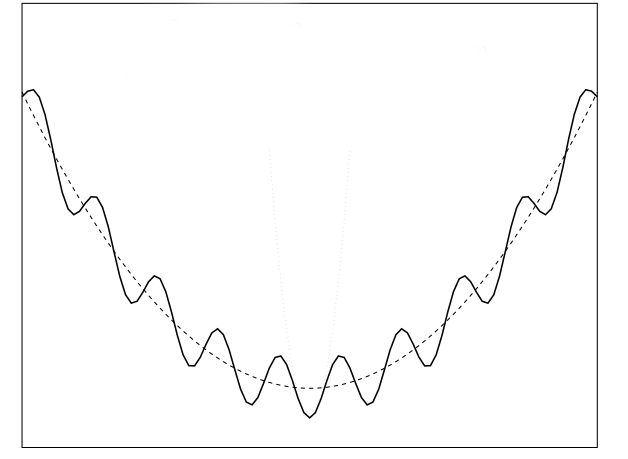
\includegraphics[trim = -1cm -3cm 0cm 0cm , clip, width=6cm,height=7cm]{Kap2/mult_min.png}%
\caption{Potencial en funci\'{o}n de la posici\'{o}n, a) mostrando la energ\'{i}a total $E$ y los cambios en la energ\'{i}a cin\'{e}tica y b) mostrando el modelo de m\'{u}ltiples m\'{i}nimos. } \label{fig:pot}
\end{figure}

Considerando la condici\'{o}n de equilibrio \eqref{eq:2} y despreciando desplazamientos de orden superior se tiene que:
\begin{equation}\label{eq:3}
V(\mathbf{q})=\frac{1}{2}\sum_{i,j=1}^{n}\frac{\partial^2 V }{\partial q_i\partial q_j}\bigg|_{\mathbf{q}=\mathbf{0}}q_i q_j
\end{equation}

Donde se identifican las constantes el\'{a}sticas como:
\begin{equation}\label{eq:4}
U_{ij}=\frac{\partial^2 V }{\partial q_i\partial q_j}\bigg|_{\mathbf{q}=\mathbf{0}}
\end{equation}

En t\'{e}rminos matriciales el potencial se puede escribir como:
\begin{equation}\label{eq:5}
V(\mathbf{q})=\frac{1}{2}\mathbf{q}^t\mathbf{U}\mathbf{q}
\end{equation}
En la ecuaci\'{o}n \eqref{eq:5} $\mathbf{q}$ es el vector columna formado por los desplazamientos de las posiciones de equilibrio para cada constituyente, i. e., $\mathbf{q}^t=(q_1,q_2,...q_n)$. Por otro lado la matriz de constantes el\'{a}sticas $\mathbf{H}$, es una matriz sim\'{e}trica debido a que la fuerza generalizada se considera conservativa, lo cual permite intercambiar el orden de las derivadas parciales.\\

Para las peque\~{n}as oscilaciones, no existen ligaduras dependientes expl\'{i}citamente de el tiempo (holon\'{o}micas) luego, la eneg\'{i}a cin\'{e}tica de los constituyentes s\'{o}lo depender\'{a} de los cuadrados de las velocidades generalizadas:
\begin{equation}\label{eq:6}
T=\frac{1}{2}\mathbf{q}^t\mathbf{M}\mathbf{q}
\end{equation}
Donde $\mathbf{M}$ es la masa generalizada, la cual se expresa en t\'{e}rminos de los factores de escala entre sistemas coordenados:
\begin{equation}\label{eq:7}
M_{jk}=\sum_{i=1}^{N} m_{i}\frac{\partial \mathbf{r_{i}} }{\partial q_j}\cdot\frac{\partial \mathbf{r_{i}} }{\partial q_k}
\end{equation}
La forma en que se escribir\'{a}n los elementos de la masa del sistema depende de la transformaci\'{o}n aplicada. Por ejemplo, en una dimensi\'{o}n las componentes de $\mathbf{q}$ se definen como:
\begin{equation}\label{eq:8}
q_i=x_i-x_{i0}
\end{equation}
En \eqref{eq:8} $x_i$ es la posici\'{o}n variable de la part\'{i}cula $i$ con respecto a un sistema fijo y $x_{i0}$ su posici\'{o}n de equilibrio. Para este caso particular \eqref{eq:7} se convierte en:
\begin{eqnarray}\label{eq:9}
M_{jk}&=&\sum_{i=1}^{N} m_{i} \delta_{ij}\delta_{ik}\nonumber \\
M_{jk}&=&m_{j} \delta_{jk}
\end{eqnarray}
La equaci\'{o}n \eqref{eq:9} dice que la matriz $\mathbf{M}$ es una matriz diagonal cuyas componentes son las masas del sistema.\\

Para el caso tridimensional, la matriz de masas del sistema es (Los detalles del c\'{a}lculo se encuentran en el anexo \ref{AnexoA}):
\begin{equation}
M_{jk}=\left( m_{3j-2}+m_{3j-1}+m_{3j} \right) \delta_{jk}
\end{equation}

\paragraph{Ecuaci\'{o}n de Movimiento}\label{par:Ecmov}
El sistema satisface la ecuaci\'{o}n de un oscilador arm\'{o}nico, lo cual se muestra para las peque\~{n}as oscilaciones en \cite[Chapter~6]{Goldstein2001}:
\begin{equation}\label{eq:14}
\mathbf{M}\ddot{\mathbf{q}}+\mathbf{U}\mathbf{q}=\mathbf{0}
\end{equation}
Para convertir la ecuaci\'{o}n a la forma est\'{a}ndar se usan las coordenadas de masa ponderada (en ingl\'{e}s mass-weighted coordinates) las cuales cambian la escala en la que se mide la posici\'{o}n:
\begin{eqnarray}\label{eq:15}
\mathbf{r}&=&\mathbf{M}^{1/2}\mathbf{q}\\
\mathbf{K}&=&\mathbf{M}^{-1/2}\mathbf{U}\mathbf{M}^{-1/2}\nonumber
\end{eqnarray}
Reemplazando dichas transformaciones en la ecuaci\'{o}n de movimiento se obtiene:
\begin{equation}\label{eq:16}
\ddot{\mathbf{r}}+\mathbf{K}\mathbf{r}=\mathbf{0}
\end{equation}
El efecto que tienen las coordenadas de masa ponderada sobre la energ\'{i}a cin\'{e}tica  es el de desaparecer la dependencia con la matriz de masas del sistema, que como se vi\'{o} puede resultar en una expresi\'{o}n tediosa. Las energias cin\'{e}tica y potencial en las nuevas coordenadas son:
\begin{eqnarray}\label{eq:19}
T&=&\frac{1}{2}\mathbf{q}^t\mathbf{M}\mathbf{q} \nonumber \\
T&=&\frac{1}{2}\mathbf{\dot{r}}^t\mathbf{M^{-1/2}}^t\mathbf{M}\mathbf{M^{1/2}}\mathbf{\dot{r}}\nonumber \\
T&=&\frac{1}{2}\mathbf{\dot{r}}^t \mathbf{\dot{r}}
\end{eqnarray}
\begin{eqnarray}\label{eq:20}
V(\mathbf{q})&=&\frac{1}{2}\mathbf{q}^t\mathbf{U}\mathbf{q} \nonumber \\
V(\mathbf{q})&=&\frac{1}{2}\mathbf{r}^t\mathbf{M^{-1/2}}^t\mathbf{U}\mathbf{M^{1/2}}\mathbf{r} \nonumber \\
V(\mathbf{q})&=&\frac{1}{2}\mathbf{r}^t\mathbf{K}\mathbf{r}
\end{eqnarray}
Una soluci\'{o}n (de prueba) a la ecuaci\'{o}n de movimiento es la oscilatoria, en la cual los constituyentes de la biomol\'{e}cula tienen la misma frecuencia $\omega$:
\begin{equation}\label{eq:17}
\mathbf{r}=\mathbf{a}e^{i\omega t}
\end{equation}
El vector $\mathbf{a}$ es denominado vector de amplitudes debido a que cada una de sus componentes corresponde a las amplitudes de cada mon\'{o}mero. Sus valores son fijos en el tiempo.\\

Al reemplazar la soluci\'{o}n de prueba en la ecuaci\'{o}n \eqref{eq:16} se convierte en un problema de autovalores y autovectores:

\begin{eqnarray}\label{eq:18}
\ddot{\mathbf{r}}&=&-\mathbf{K}\mathbf{r} \nonumber \\
\omega^2\mathbf{a}&=&\mathbf{K}\mathbf{a} \nonumber \\
\lambda_{k}\mathbf{a_{k}}&=&\mathbf{K}\mathbf{a_{k}}
\end{eqnarray}

En \eqref{eq:18} se ha definido $\lambda=\omega^2$ y posteriormente se ha agregado el sub\'{i}ndice $k$ para distinguir cada uno de los autovalores y autovectores que se encuentren en el problema \eqref{eq:18}.\\
Cuando cada uno de los mon\'{o}meros tiene la misma frecuencia, a cada frecuencia le corresponde un vector de amplitudes $\mathbf{a}$, cada uno de estos posibles vectores se les conoce como un \textit{modo normal de oscilaci\'{o}n}.\\

Ha de notarse que la soluci\'{o}n total no est\'{a} compuesta por un \'{u}nico modo, sino por la superposici\'{o}n de estos:
\begin{equation}\label{eq:tot}
\mathbf{r}=\sum_k\mathbf{a}_ke^{i\omega_k t}
\end{equation}

Cuando se tiene esta soluci\'{o}n y se desean conocer los modos normales, pueden aplicarse dos m\'{e}todos: El de la transformada de Fourier para conocer las frecuencias y la transformaci\'{o}n a las coordenadas normales; las coordenadas normales son un espacio en el cual se separan los movimientos compuestos.\\

Las coordenadas normales $\mathbf{\zeta}$ se definen como:
\begin{equation}
\mathbf{r}=\mathbf{T}\mathbf{\zeta}
\end{equation}
Donde $\mathbf{T}$ es una transformaci\'{o}n ortogonal  $\mathbf{T}\mathbf{T}^T=\mathbf{I}$ formada por los modos normales $\mathbf{a}_k$  pero modificados para que se cumpla la ortonormalidad. Cada componente de $\mathbf{\zeta}$ es:
\begin{equation}\label{eq:nor}
\zeta_k=C_k e^{i\omega_k t}
\end{equation}
Es decir, las coordenadas normales $\zeta_k$ representan a un \'{u}nico modo normal de oscilaci\'{o}n, una \'{u}nica frecuencia. Mientras que las columnas de $\mathbf{T}$ proporcionan las direcciones en las que se da cada modo normal.\\


\subsubsection{Ensamble Estad\'{i}stico}
Cuando el sistema (biomol\'{e}cula) se encuentre a temperaturas fisiol\'{o}gicas, s\'{o}lo intercambiar\'{a} calor con los alrededores (ba\~{n}o t\'{e}rmico). Sin embargo, se ha demostrado  que a esta temperatura, la aproximaci\'{o}n arm\'{o}nica falla , \cite{Hayward2008}; por otro lado, a temperatura fisiol\'{o}gica el ensamble es cl\'{a}sico dependiendo del rango de frecuencias a analizar\cite{Sethna2006}, \cite{Cui2006}. En la figura \ref{fig:estad}, se observa el n\'{u}mero de nodos en funci\'{o}n de la frecuencia para diferentes prote\'{i}nas, para frecuencias menores que la frecuencia de vibraci\'{o}n del oscilador arm\'{o}nico a temperatura ambiente, se puede trabajar con la mec\'{a}nica cl\'{a}sica.\\
\begin{figure}
\centering%
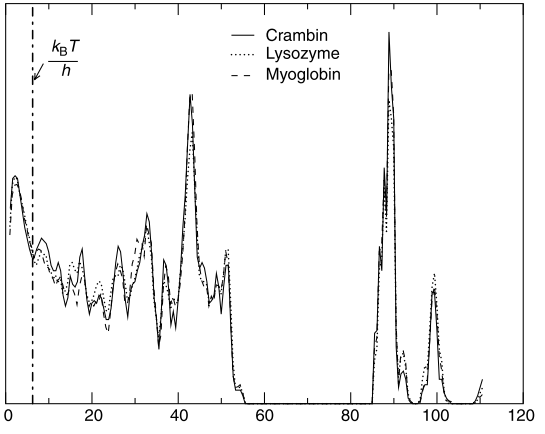
\includegraphics[scale=0.3]{Kap2/modos_vs_f.png}%
\put(-65,5){\rotatebox{90}{N\'{u}mero de modos}}
\put(-45,-5){Frecuencia ($p\mathrm{s}^{-1}$)}
\caption{N\'{u}mero de modos normales en funci\'{o}n de la frecuencia para tres prote\'{i}nas diferentes.$k_BT/h$ es la frecuencia correspondiente a la m\'{a}s baja energ\'{i}a promedio a temperatura $T$. Tomado de \cite{Cui2006}.} \label{fig:estad}
\end{figure}
Como \'{u}nicamente hay intercambio de energ\'{i}a y se trabaja a temperatura fisiol\'{o}gica, la estad\'{i}stica apropidada es la del ensamble can\'{o}nico. En el ensamble  can\'{o}nico se sigue la distribuci\'{o}n de probabilidad de Boltzmann:
\begin{equation}\label{eq:21}
\rho=\frac{\exp(-E_s/k_BT)}{Z}
\end{equation}
Donde $E_s$ es la energ\'{i}a del sistema y $Z$ la funci\'{o}n de partici\'{o}n. La funci\'{o}n de partici\'{o}n es el factor de normalizaci\'{o}n de la densidad de probabilidad y cuenta todos los posibles microestados a temperatura constante:
\begin{equation}\label{eq:22}
Z=\frac{1}{h^{n}}\int \mathrm{d}^n p\mathrm{d}^n q \exp \left [-H(\mathbf{p},\mathbf{q})/k_BT \right]
\end{equation}
En \eqref{eq:22}, $n=3N$ cuando el n\'{u}mero de coordenadas $q_i$ escogido es el mismo que el n\'{u}mero de coordenadas cartesianas.\\
Ha de notarse que la funci\'{o}n de partici\'{o}n en \eqref{eq:22} desacopla los momentos y las posiciones, ya que el hamiltoniano est\'{a} dado por la f\'{o}rmula $H=T+V$, donde la enger\'{i}a cin\'{e}tica depende s\'{o}lo de los momentos generalizados y  el potencial de las coordenadas generalizadas.\\

Se desarrolla \eqref{eq:22} teniendo en cuenta que $\mathbf{M}$ es diagonal:
\begin{eqnarray}\label{eq:23}
Z&=&\frac{1}{h^{n}}\int \mathrm{d}^n p\mathrm{d}^n q \exp \left [-\left( \mathbf{\dot{q}^t}\mathbf{M}\mathbf{\dot{q}}/2+\mathbf{q}^t\mathbf{U}\mathbf{q}/2\right)/k_BT \right]
\nonumber \\
Z&=&\frac{1}{h^{n}}\int \mathrm{d}^n p \exp \left [-\sum_i \frac{p_i^2}{2m_i}\right]
\int \mathrm{d}^n r \left( \prod_i \sqrt{m_i}\right)\exp \left[-\frac{1}{2}\mathbf{r}^t\mathbf{K}\mathbf{r}/k_BT \right]
\nonumber \\
Z&=&\frac{(2\pi)^{n/2}}{h^{n}}
\int \mathrm{d}^n r\exp \left[-\frac{1}{2}\mathbf{r}^t\mathbf{K}\mathbf{r}/k_BT \right] 
\end{eqnarray}
El resultado \eqref{eq:23} es el mostrado en \cite{Lezon2009} o en \cite{Sethna2006}:
\begin{equation}\label{eq:24}
Z=\frac{\left(k_BT\right)^{n/2}}{\hbar^{n}} \frac{1}{|\mathbf{K}|^{n/2}}
\end{equation}
Tomando $\hbar=1$ y teniendo en cuenta que el determinante de $\mathbf{K}$ es el producto de los autovalores no nulos, es decir, de las frecuencias al cuadrado:
\begin{eqnarray}\label{eq:25}
Z&=&\left(k_BT\right)^{n/2} \prod_{i=1}^{n}\frac{1}{\omega_i}
 \\
Z&=&\left(k_BT\right)^{n/2} |\mathbf{K^{-1}}|^{1/2}
\end{eqnarray}
Se observa que los modos de m\'{a}s bajas frecuencias contribuyen m\'{a}s a la funci\'{o}n de partici\'{o}n.
\section{Descripciones de los Movimientos Globales}
\subsection{ENMs}
\subsubsection{Modelos de Redes Anisotr\'{o}picas (ANM)}\label{ssec:ANM}
Como se ha dicho, la aproximaci\'{o}n a segundo orden del potencial, minimizaci\'{o}n, \eqref{eq:5} es cambiada por un potencial de Hooke en el cual se tienen en cuenta las distancias en lugar de los desplazamientos alrededor del equilibrio y tambi\'{e}n se pueden tener en cuenta diferentes constantes el\'{a}sticas entre diferentes nodos:
\begin{equation}\label{eq:26}
V=
   \frac{1}{2}\sum_{
   i,j>i  
   }
   \gamma_{ij}\left(R_{ij}-R_{ij}^0\right)^2
\end{equation}
\begin{equation*}
\mbox{			Con		} R_{ij},R_{ij}^0<R_c  
\end{equation*}

Donde $R_{ij}^0$ es la distancia de equilibrio entre los nodos $i-j$ de la red, $R_{ij}$ su distancia variable y $\gamma_{ij}$ las constantes el\'{a}sticas entre los nodos $i-j$. Como se ilustra en la figura \ref{fig:res}, el t\'{e}rmino $R_{ij}-R_{ij}^0$ es la elongaci\'{o}n del resorte, lo cual es diferente a la resta de los desplazamientos, ecuaci\'{o}n \eqref{eq:3}; entonces no se est\'{a} aproximando el potencial ni se requiere una minimizaci\'{o}n de la energ\'{i}a, como se ha recalcado, s\'{o}lo se cambia la forma del potencial.\\

Se requiere que $j>i$ para que no aparezca repetido el t\'{e}rmino $\left(R_{ij}-R_{ij}^0\right)^2$ con $\left(R_{ji}-R_{ji}^0\right)^2$   ya que representan la misma interacci\'{o}n, de ser as\'{i}, se vuelven obsoletas las constantes el\'{a}sticas $\gamma_{ij}$ con $j<i$. Sin embargo, el potencial tambi\'{e}n puede escogerse dejando los t\'{e}rminos repetidos y redefiniendo la matriz de constantes el\'{a}sticas como una matriz sim\'{e}trica, esto es: $\gamma_{ij}=\gamma_{ji}$. Escogiendo el potencial de esta manera, como es usal en la literatura \cite{Rader2006}, queda de la forma:
\begin{equation}\label{eq:26}
V_{ANM}=
   \frac{1}{2}\sum_{
   i\neq j=1  z
   }
   \gamma\left(R_{ij}-R_{ij}^0\right)^2
\end{equation}
\begin{eqnarray*}
\mbox{			Con		} R_{ij},R_{ij}^0<R_c \\
\mbox{			y		} \gamma_{ij}=\gamma_{ji}
\end{eqnarray*}
\begin{figure}
\centering%
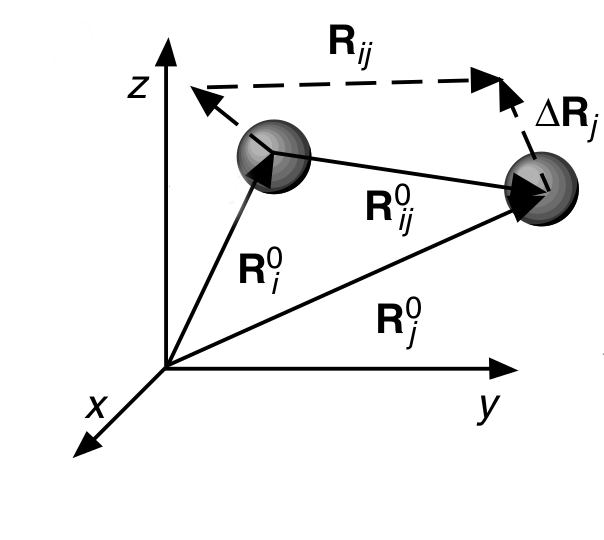
\includegraphics[scale=0.3]{Kap2/resorte.png}%
\caption{Desplazamientos de los nodos $i-j$ de su posici\'{o}n de equilibrio. Tomado de \cite{Rader2006}.} \label{fig:res}
\end{figure}
Existe un servidor web \cite{Eyal2015} basado en ANM que permite ver los movimientos globales de una prote\'{i}na o de un \'{a}cido nucleico y permite obtener informaci\'{o}n como los autovalores, los factores-B, las correlaciones entre otras.\footnote{ Recurso disponible en \url{http://anm.csb.pitt.edu/cgi-bin/anm2/anm2.cgi}}
\paragraph{Matriz Hessiana}\label{par:Mhes}
El c\'{a}lculo de la matriz de segundas derivadas $\mathbf{U}$ para el an\'{a}lisis de modos normales, si parte de una minimizaci\'{o}n de la energ\'{i}a.  Las derivadas se calculan v\'{i}a el potencial anisotr\'{o}pico \eqref{eq:26}, para el presente caso la matriz $\mathbf{U}$ es llamada $\mathbf{\mathcal{H}}$. La matriz $\mathbf{\mathcal{H}}$ es de tama\~{n}o $3N\times3N$ con $N$ el n\'{u}mero de residuos y est\'{a} constituida por $N\times N$ submatrices de tama\~{n}o $3\times3$ llamadas $\mathbf{H}_{ij}$:
\begin{equation}\label{eq:34}
\mathbf{\mathcal{H}}=\{H_{ij}\} \mbox{		con	}i,j=1,...,N
\end{equation}
Los elementos de $\mathbf{H}_{ij}$ son:
\begin{equation}\label{eq:35}
\mathbf{H}_{ij}=\left(
\begin{array}{ccc}
 \partial_{xi}\partial_{xj} V & \partial_{xi}\partial_{yj} V & \partial_{xi}\partial_{zj} V \\
 \partial_{yi}\partial_{xj} V & \partial_{yi}\partial_{yj} V & \partial_{yi}\partial_{zj} V \\
 \partial_{zi}\partial_{xj} V & \partial_{zi}\partial_{yj} V & \partial_{zi}\partial_{zj} V
\end{array}
\right)
\end{equation}

Calculando algunas de estas derivadas y definiendo $x_{ik}=x_k-x_i$, $y_{ik}=y_k-y_i$ y $z_{ik}=z_k-z_i$ se obtiene (Caso $i\neq j$):
\begin{equation}\label{eq:36}
\frac{\partial V }{\partial y_k}=\sum_j\frac{\gamma_{jk}\left(R_{kj}-R_{kj}^0\right)y_{kj}}{R_{kj}}
\end{equation}
\begin{equation}\label{eq:37}
\frac{\partial^2 V }{\partial x_i\partial y_j}\bigg|_{R_{ij}=R_{ij}^0}=-\frac{\gamma_{ij}x_{ij}y_{ij}}{R_{ij}^2}
\end{equation}
\begin{equation}\label{eq:38}
\frac{\partial^2 V }{\partial x_i\partial x_j}\bigg|_{R_{ij}=R_{ij}^0}=-\frac{\gamma_{ij}x_{ij}^2}{R_{ij}^2}
\end{equation}
De forma an\'{a}loga se encuentran los otros elementos de $\mathbf{H}_{ij}$ con lo cual los superelementos no diagonales de $\mathbf{\mathcal{H}}$ quedan escritos como \cite{Lezon2009}:
\begin{equation}\label{eq:35}
\mathbf{H}_{ij}=-\frac{\gamma_{ij}}{R_{ij}^2}\left(
\begin{array}{ccc}
 x_{ij}^2 & x_{ij}y_{ij} & x_{ij}z_{ij}\\
 y_{ij}x_{ij} & y_{ij}^2 & y_{ij}z_{ij} \\
 z_{ij}x_{ij} &z_{ij}y_{ij} & z_{ij}^2
\end{array}
\right)
\end{equation}


Para los superelementos $\mathbf{H}_{ii}$ que se encuentran en la diagonal, algunos de sus elementos son:
\begin{eqnarray}\label{eq:39}
\frac{\partial^2 V }{\partial x_i^2}\bigg|_{R_{ij}=R_{ij}^0}=-\sum_{j\neq i}\gamma_{ij}\left(\frac{x_{ij}^2}{R_{ij}^2}\right) \nonumber \\
\frac{\partial^2 V }{\partial x_i^2}\bigg|_{R_{ij}=R_{ij}^0}=-\sum_{j\neq i} H_{ij,xx}
\end{eqnarray}
En \eqref{eq:39}, $H_{ij,xx}$ es el primer elemento de la submatriz $\mathbf{H}_{ij}$. El resultado \eqref{eq:39} puede generalizarse para todos los superelementos de la diagonal, ver \cite{Lezon2009}:
\begin{eqnarray}\label{eq:40}
\mathbf{H}_{ii}=\sum_{j\neq i}\mathbf{H}_{ij}
\end{eqnarray}
Una vez obtenida la matriz Hessiana, es necesario calcular sus autovalores y autovactores de la misma forma que en NMA, ya que esto describe los movimientos de la biomol\'{e}cula. La diagonalizaci\'{o}n de $\mathcal{H}$ lleva a lo sumo $3N-6$ modos normales no nulos, como se demuestra en \cite{Tirion1996}. Los 6 modos normales restantes, corresponden a las rotaciones y traslaciones de un cuerpo r\'{i}gido; se puede escoger un sistema fijo en la molecula y que rote con ella.\\

El t\'{e}rmino de la distancia de corte $R_c$ puede ser incluido en las constantes el\'{a}sticas, es decir, $\gamma_{ij}=0$ si  $R_{ij}>R_c$ sino $\gamma_{ij}\neq 0$. Adicional a esto, las constantes el\'{a}sticas pueden ser iguales (isotr\'{o}picas): $\gamma_{ij}=\gamma$ si  $R_{ij}<R_c$ de lo contrario  $\gamma_{ij}=0$.
\subsubsection{Modelo de Redes Gaussianas (GNM)}\label{ssec:GNM}
El modelo se denomina gaussiano debido a que las desviaciones del equilibrio o fluctuaciones son isotr\'{o}picas y siguen una distribuci\'{o}n gaussiana \cite{Rader2006}. Se requieren dos par\'{a}metros para describir el modelo: Una misma constante el\'{a}stica $\gamma$ para todas las unidades de la biomol\'{e}cula y una distancia de corte a partir de la cual no se ejerce el potencial.\\

Contrario al ANM, en el modelo de redes gaussianas se consideran las desviaciones del equilibrio como desplazamientos:
\begin{equation}\label{eq:27}
V_{GNM}=\frac{\gamma}{2}\sum_{i,j=1}^{N}\Gamma_{ij}\left(\textbf{R}_{ij}-\textbf{R}_{ij}^0\right)^2
\end{equation}
Al ser $\gamma_{ij}$ una matriz de constantes el\'{a}sticas, se incluyen en la sumatoria los elementos $\Gamma_{ij}$ donde $\gamma_{ij}=\gamma\Gamma_{ij}$. $\Gamma_{ij}$ representa la simetr\'{i}a de la matriz $ \mathbf{\gamma}$ y como se puede ver en \cite{Rader2006}, la topolog\'{i}a de la red.\\

Ya que $\textbf{R}_{ij}=\textbf{R}_{j}-\textbf{R}_{i}$ y definiendo $\Delta\textbf{R}_{i}=\textbf{R}_{i}-\textbf{R}_{i}^0$ se tiene que  $\textbf{R}_{ij}-\textbf{R}_{ij}^0=\Delta\textbf{R}_{j}-\Delta\textbf{R}_{i}$, el potencial gaussiano se puede escribir en t\'{e}rminos de los desplazamientos individuales:
\begin{eqnarray}\label{eq:34}
V_{GNM}&=&\frac{\gamma}{2}\sum_{i\neq j=1}^{N}\Gamma_{ij}\left( \Delta\textbf{R}_{j}-\Delta\textbf{R}_{i}\right)^2 \nonumber \\
V_{GNM}&=&\frac{\gamma}{2}\sum_{i\neq j=1}^{N}\Gamma_{ij}\left[\left(\Delta x_j-\Delta x_i \right)^2+\left(\Delta y_j-\Delta y_i \right)^2+\left(\Delta z_j-\Delta z_i \right)^2 \right] \nonumber \\
V_{GNM}&=&\frac{\gamma}{2}\sum_{i\neq j=1}^{N}\Gamma_{ij}\left[\left(\Delta x_{ij}\right)^2+\left(\Delta y_{ij}\right)^2+\left(\Delta z_{ij}\right)^2 \right]
\end{eqnarray}
Escribiendo \eqref{eq:34} en forma matricial se tiene:
\begin{equation}\label{eq:35}
V_{GNM}=\frac{\gamma}{2}\left(\Delta\mathbf{X}^T\mathbf{\Gamma}\Delta\mathbf{X}+\Delta\mathbf{Y}^T\mathbf{\Gamma}\Delta\mathbf{Y}+\Delta\mathbf{Z}^T\mathbf{\Gamma}\Delta\mathbf{Z} \right)
\end{equation}
Con $\Delta\mathbf{X}^T$ un vector $N$ dimensional con componentes:$\Delta\mathbf{X}^T=\left(\Delta x_1,...,\Delta x_N\right)$ y $\mathbf{\Gamma}$ la matriz de Kirchhoff que se discutir\'{a} en o que sigue con el fin de entender la expresi\'{o}n \eqref{eq:35}.\\

Para garantizar que $\Gamma_{ij}$ sea adimensional, se escogen (no de forma \'{u}nica) los elementos fuera de la diagonal de acuerdo al procedimiento descrito a continuaci\'{o}n.\\

N\'{o}tese que los t\'{e}rminos cuadr\'{a}ticos por cada componente pueden expandirse:
\begin{eqnarray}\label{eq:36}
\sum_{i\neq j=1}^{N}\Gamma_{ij}\left(\Delta x_{ij}\right)^2&=&\sum_{i\neq j=1}^{N}\Gamma_{ij}\left(\Delta x_{i}^2+\Delta x_{j}^2-2\Delta x_{i}\Delta x_{j}\right) \nonumber \\
&=&2\sum_{i\neq j=1}^{N}\Gamma_{ij}\Delta x_{i}^2-2\sum_{i\neq j=1}^{N}\Delta x_{i}\Gamma_{ij}\Delta x_{j}
\end{eqnarray}

La idea es que los t\'{e}rminos de \eqref{eq:36} y \eqref{eq:35} coincidan. Escribiendo expl\'{i}citamente el t\'{e}rmino de la componente x en \eqref{eq:35}:
\begin{eqnarray}\label{eq:37}
editar
\end{eqnarray}
De lo anterior se concluye que la matriz de de Kirchhoff $\mathbf{\Gamma}$ es:
\begin{equation}\label{eq:38}
\Gamma_{ij}=\left\{\begin{array}{ccc}
-1 &\mbox{si }i\neq j&\mbox{	y	}R_{ij}\leq r_c \\
0&\mbox{si }i\neq j&\mbox{	y	}R_{ij}\geq r_c \\
-\sum_{j,j\neq i}\Gamma_{ij}&\mbox{si	}i=j&.\\
            \end{array}
\right.
\end{equation}

\paragraph{Fluctuaciones, Correlaciones}.\\
El objetivo primario es calcular las fluctuaciones cuadr\'{a}ticas medias (ms por sus siglas en ingl\'{e}s) para un residuo y las correlaciones entre residuos. Las fluctuaciones ms proporcionan los movimientos de la biomol\'{e}cula y las correlaciones establecen la dependencia entre distintas partes de la biomol\'{e}cula, es decir, los movimientos colectivos.\\

Las fluctuciones ms para el residuo $i$ se calculan como:
\begin{equation}\label{eq:39}
\langle\Delta \mathbf{R_i}\cdot\Delta\mathbf{R_i}\rangle=\langle\Delta{X_i}^2\rangle+\langle\Delta {Y_i}^2\rangle +\langle\Delta {Z_i}^2\rangle 
\end{equation}

Y las correlaciones entre el residuo $i$ y el $j$ son:
\begin{equation}\label{eq:40}
\langle\Delta \mathbf{R_i}\cdot\Delta\mathbf{R_j}\rangle=\langle\Delta X_i\Delta X_j\rangle+\langle\Delta Y_i\Delta Y_j\rangle +\langle\Delta Z_i\Delta Z_j\rangle 
\end{equation}
Los promedios calculados en \eqref{eq:39} y en \eqref{eq:40} son calculados con respecto al espacio de coordenadas.\\

De manera similar al resultado \label{eq:25}, donde la matriz $\mathbf{K}$ es cambiada por la matriz $\gamma\mathbf{\Gamma}$ y $n=3N$ se llega a la funci\'{o}n de partici\'{o}n gaussiana:
\begin{equation}\label{eq:41}
Z_{GNM}=\left(2\pi\right)^{3N/2}\left| \frac{k_BT}{\gamma}\Gamma^{-1}\right|^{1/2}
\end{equation}

En \cite{Rader2006} se encuentra que estas medidas est\'{a}n relacionadas con la inversa de la matriz de Kirchhoff:\\
\begin{equation}\label{eq:42}
\langle \Delta \mathbf{R_i}^2 \rangle=\frac{3 k_BT}{\gamma}\left(\mathbf{\Gamma}^{-1}\right)_{ii}
\end{equation}
\begin{equation}\label{eq:43}
\langle \Delta \mathbf{R_i}\cdot\Delta \mathbf{R_j} \rangle=\frac{3 k_BT}{\gamma}\left(\mathbf{\Gamma}^{-1}\right)_{ij}\\
\end{equation}
\paragraph{Factor-B}.\\
El factor-B, factor de Debye-Waller o factor de temperatura es un factor que est\'{a} directamente relacionado con las amplitudes de los haces dispersados cuando se hace difracci\'{o}n de rayos-x y por lo tanto describe la atenuaci\'{o}n de la dispersi\'{o}n.\\

Para un modelo de arm\'{o}nico isotr\'{o}pico, donde cada constituyente fluct\'{u}a de su posici\'{o}n de equilibrio como: $\mathbf{\Delta R_{i}}=R_i-R_i^0$, se encuentra que la intensidad de onda dispersada es:
\begin{equation}\label{eq:44}
I=I_0\exp\left(-\frac{1}{3}\langle\mathbf{\Delta R_{i}}\rangle^2 \mathbf{q}^2\right)
\end{equation}
Con $\mathbf{q}$ el vector de la red rec\'{i}proca, $I_0$ la intensidad dispersada para la estrucutura r\'{i}gida\\

El \textit{factor B} se define como el t\'{e}rmino dentro de la exponencial en \eqref{eq:44}. Como est\'{a} directamente relacionado con la fluctuaci\'{o}n ms, entonces es una \textit{medida de la rigidez o de la flexibilidad} de la biomol\'{e}cula, adem\'{a}s tiene unidades de $\AA^2$:
\begin{equation}\label{eq:45}
I=-\frac{1}{3}\langle\mathbf{\Delta R_{i}}\rangle^2 \mathbf{q}^2
\end{equation}
En la dispersi\'{o}n de Bragg, el vector de onda de la red rec\'{i}proca es $4\pi\sin\theta/\lambda$. Tomando la aproximaci\'{o}n de \'{a}ngulos peque\~{n}os $\cos \theta\sim \theta$, el factor B se convierte en:
\begin{equation}\label{eq:46}
B=\frac{8\pi}{3}\langle\mathbf{\Delta R_{i}}\rangle^2
\end{equation}
Para el caso del GNM y de acuerdo a \eqref{eq:42}, el factor de estructura se convierte en:
\begin{equation}\label{eq:47}
B=\frac{8\pi^2 k_BT}{\gamma}\left(\mathbf{\Gamma}^{-1}\right)_{ii}
\end{equation}
Existe un servidor web basado en GNM que permite ver los movimientos globales de una prote\'{i}na o de un \'{a}cido nucleico y permite obtener informaci\'{o}n como los autovalores, los factores-B, las correlaciones entre otras.\footnote{ Recurso disponible en \url{http://gnm.csb.pitt.edu/index.php}}

\subsection{An\'{a}lisis por Componentes Principales (PCA)}
Sea $\mathbf{x(t)}$ la trayectoria en forma de vector columna de $3N$ componentes que tiene las posiciones a cada instante de tiempo de todos los \'{a}tomos. La matriz de covarianza, en este caso, es aqu\'{e}lla que mide la dependencia entre cada una de las variables ($3N$ componentes) y cuyos elementos de la diagonal son las varianzas de dichas variables.\\

Matriz de covarianza:
\begin{equation}\label{eq:28}
\mathbf{C}=\langle(\mathbf{x(t)}-\langle\mathbf{x}\rangle)(\mathbf{x(t)}-\langle\mathbf{x}\rangle)^T\rangle
\end{equation}

En \eqref{eq:29}, la media es calculada para la trayectoria en todos los tiempos.\\
La matriz de covarianza puede ser expresada en t\'{e}rminos de sus autovalores  $\lambda_i$ y sus autovectores $\mathbf{t_i}$, con $i<3N+1$.
\begin{equation}\label{eq:48}
\mathbf{C}\mathbf{t_i}=\lambda_i\mathbf{t_i}
\end{equation}
Tomando $\Lambda={\lambda_i}$, la matriz diagonal formada por los autovalores y $\mathbf{T}=\left(\mathbf{t_1},\mathbf{t_2},...,\mathbf{t_{3N}}\right)$ como la matriz cuyas columnas son los autovectores, escritas de tal manera que los autovalores esten ordenados de mayor a menor y los autovectores ordenados de acuerdo a los autovalores entonces:
\begin{equation}\label{eq:29}
\mathbf{\Lambda}=\mathbf{T}^T\mathbf{C}\mathbf{T}
\end{equation}
Donde se ha tenido en cuenta que $\mathbf{T}^{-1}=\mathbf{T}^T$. Expresado de otra forma:
\begin{equation}\label{eq:30}
\mathbf{C}=\mathbf{T}\mathbf{\Lambda} \mathbf{T}^T
\end{equation}
La esencia de un PCA es descartar los modos menos relevantes que corresponden a los autovalores m\'{a}s peque\~{n}os y generar un nuevo conjunto de datos de menor tama\~{n}o a partir de estos (componentes principales). En \cite{Amadei1993} se demuestra que las desviaciones m\'{a}s grandes corresponden a los autovalores m\'{a}s grandes, por tanto, se trabaja s\'{o}lamente con los autovalores m\'{a}s grandes. \\

Dejando s\'{o}lamente en $\mathbf{T}$ los $M$ autovectores o columnas m\'{a}s relevantes, se define la matriz de las componentes principales $\mathbf{P}=\left(\mathbf{p_1},\mathbf{p_2},...,\mathbf{p_{M}}\right)$, donde $M<3N$ como:
\begin{eqnarray}\label{eq:31}
\mathbf{P}&=&\mathbf{T}^T(\mathbf{x(t)}-\langle\mathbf{x}\rangle)^T \nonumber \\
\mathbf{P}&=&(\mathbf{x(t)}-\langle\mathbf{x}\rangle)\mathbf{T}
\end{eqnarray}
O en t\'{e}rminos de cada componente principal:
\begin{equation}\label{eq:32}
\mathbf{p_i}=\mathbf{t_i}^T(\mathbf{x(t)}-\langle\mathbf{x}\rangle)^T
\end{equation}
Si se desea volver a los datos originales hay que realizar la transformaci\'{o}n inversa:
\begin{equation}\label{eq:33}
\mathbf{x(t)}^T=\mathbf{T}\mathbf{P}+\langle\mathbf{x}\rangle^T
\end{equation}
\subsection{Modelos de Bloque R\'{i}gido (BNM o RTB)}
Los modos normales de los bloques r\'{i}gidos tienen una dimensi\'{o}n de tama\~{n}o $n_b$ con respecto a los de un NMA, $3N$. Los modos normales de bloque r\'{i}gido se definen a partir de una transformaci\'{o}n denominada $\mathbf{P}$ del espacio de las ${q_i}$ al de los bloques r\'{i}gidos $r_i'$.\\

\section{Clasificaci\'{o}n de los Modos Normales}
\begin{figure}
\centering%
%%LaTeX with PSTricks extensions
%%Creator: inkscape 0.48.5
%%Please note this file requires PSTricks extensions
\psset{xunit=.5pt,yunit=.5pt,runit=.5pt}
\begin{pspicture}(431.03445435,1066.43151855)
{
\newrgbcolor{curcolor}{0 0 0}
\pscustom[linestyle=none,fillstyle=solid,fillcolor=curcolor]
{
\newpath
\moveto(11.49576477,336.38147466)
\lineto(18.75162414,333.70569341)
\lineto(18.75162414,339.06702154)
\lineto(11.49576477,336.38147466)
\moveto(9.55240539,335.26819341)
\lineto(9.55240539,337.50452154)
\lineto(24.13248352,343.06116216)
\lineto(24.13248352,341.01038091)
\lineto(20.39224914,339.68225591)
\lineto(20.39224914,333.10999029)
\lineto(24.13248352,331.78186529)
\lineto(24.13248352,329.70178716)
\lineto(9.55240539,335.26819341)
}
}
{
\newrgbcolor{curcolor}{0 0 0}
\pscustom[linestyle=none,fillstyle=solid,fillcolor=curcolor]
{
\newpath
\moveto(17.53092102,354.19397466)
\lineto(24.13248352,354.19397466)
\lineto(24.13248352,352.39709966)
\lineto(17.58951477,352.39709966)
\curveto(16.55436609,352.39709048)(15.77962729,352.19526777)(15.26529602,351.79163091)
\curveto(14.75098248,351.38797691)(14.49382128,350.78250877)(14.49381164,349.97522466)
\curveto(14.49382128,349.00516679)(14.80306576,348.2401936)(15.42154602,347.68030279)
\curveto(16.04004369,347.12040305)(16.88314181,346.84045542)(17.95084289,346.84045904)
\lineto(24.13248352,346.84045904)
\lineto(24.13248352,345.03381841)
\lineto(13.19498352,345.03381841)
\lineto(13.19498352,346.84045904)
\lineto(14.89420227,346.84045904)
\curveto(14.23666008,347.27014249)(13.74512411,347.77469927)(13.41959289,348.35413091)
\curveto(13.0940831,348.94006269)(12.93132284,349.61389014)(12.93131164,350.37561529)
\curveto(12.93132284,351.63211729)(13.32194745,352.58263717)(14.10318664,353.22717779)
\curveto(14.87793548,353.87169838)(16.02051246,354.19396369)(17.53092102,354.19397466)
}
}
{
\newrgbcolor{curcolor}{0 0 0}
\pscustom[linestyle=none,fillstyle=solid,fillcolor=curcolor]
{
\newpath
\moveto(9.55240539,357.57288091)
\lineto(25.98795227,362.65100591)
\lineto(25.98795227,360.99084966)
\lineto(9.55240539,355.91272466)
\lineto(9.55240539,357.57288091)
}
}
{
\newrgbcolor{curcolor}{0 0 0}
\pscustom[linestyle=none,fillstyle=solid,fillcolor=curcolor]
{
\newpath
\moveto(9.55240539,366.25452154)
\lineto(14.97232727,366.25452154)
\lineto(14.97232727,364.59436529)
\lineto(9.55240539,364.59436529)
\lineto(9.55240539,366.25452154)
}
}
{
\newrgbcolor{curcolor}{0 0 0}
\pscustom[linestyle=none,fillstyle=solid,fillcolor=curcolor]
{
\newpath
\moveto(25.98795227,378.40295904)
\lineto(27.39420227,378.40295904)
\lineto(27.39420227,377.79749029)
\curveto(27.394199,376.17638854)(27.15331383,375.08915004)(26.67154602,374.53577154)
\curveto(26.18977312,373.98889073)(25.22948763,373.7154535)(23.79068664,373.71545904)
\lineto(21.45670227,373.71545904)
\curveto(20.47363301,373.7154535)(19.79329515,373.53967243)(19.41568664,373.18811529)
\curveto(19.03808757,372.83654813)(18.84928567,372.19852794)(18.84928039,371.27405279)
\lineto(18.84928039,370.67834966)
\lineto(17.45279602,370.67834966)
\lineto(17.45279602,371.27405279)
\curveto(17.4528027,372.20503835)(17.26725601,372.84305854)(16.89615539,373.18811529)
\curveto(16.51855884,373.53967243)(15.84473139,373.7154535)(14.87467102,373.71545904)
\lineto(12.53092102,373.71545904)
\curveto(11.09213197,373.7154535)(10.13510168,373.98889073)(9.65982727,374.53577154)
\curveto(9.17807139,375.08915004)(8.93718621,376.17638854)(8.93717102,377.79749029)
\lineto(8.93717102,378.40295904)
\lineto(10.33365539,378.40295904)
\lineto(10.33365539,377.73889654)
\curveto(10.33366919,376.82091915)(10.47689821,376.22196141)(10.76334289,375.94202154)
\curveto(11.04981431,375.66206614)(11.65202725,375.52209232)(12.56998352,375.52209966)
\lineto(14.99185852,375.52209966)
\curveto(16.01400205,375.52209232)(16.75618881,375.37235289)(17.21842102,375.07288091)
\curveto(17.68066705,374.77990556)(17.99316674,374.27534878)(18.15592102,373.55920904)
\curveto(18.33170807,374.28185919)(18.65071816,374.78967118)(19.11295227,375.08264654)
\curveto(19.57519641,375.37560809)(20.31412796,375.52209232)(21.32974914,375.52209966)
\lineto(23.75162414,375.52209966)
\curveto(24.66959235,375.52209232)(25.27180529,375.66206614)(25.55826477,375.94202154)
\curveto(25.84472139,376.22196141)(25.98795041,376.82091915)(25.98795227,377.73889654)
\lineto(25.98795227,378.40295904)
}
}
{
\newrgbcolor{curcolor}{0 0 0}
\pscustom[linestyle=none,fillstyle=solid,fillcolor=curcolor]
{
\newpath
\moveto(18.63443664,387.76819341)
\curveto(18.63444214,386.31636509)(18.8004576,385.31050672)(19.13248352,384.75061529)
\curveto(19.46451943,384.19071618)(20.03092512,383.91076854)(20.83170227,383.91077154)
\curveto(21.46972576,383.91076854)(21.97753775,384.11910167)(22.35513977,384.53577154)
\curveto(22.72623492,384.95894458)(22.91178161,385.53186067)(22.91178039,386.25452154)
\curveto(22.91178161,387.25060895)(22.56021946,388.0481342)(21.85709289,388.64709966)
\curveto(21.14746046,389.25256007)(20.20670619,389.55529415)(19.03482727,389.55530279)
\lineto(18.63443664,389.55530279)
\lineto(18.63443664,387.76819341)
\moveto(17.89224914,391.35217779)
\lineto(24.13248352,391.35217779)
\lineto(24.13248352,389.55530279)
\lineto(22.47232727,389.55530279)
\curveto(23.13639076,389.14513831)(23.62792673,388.63407111)(23.94693664,388.02209966)
\curveto(24.25943651,387.410114)(24.41568636,386.66141683)(24.41568664,385.77600591)
\curveto(24.41568636,384.6562105)(24.10318667,383.76428431)(23.47818664,383.10022466)
\curveto(22.84667751,382.44267105)(22.00357939,382.11389534)(20.94888977,382.11389654)
\curveto(19.71842543,382.11389534)(18.79069198,382.52405118)(18.16568664,383.34436529)
\curveto(17.54069323,384.17118495)(17.22819354,385.40165247)(17.22818664,387.03577154)
\lineto(17.22818664,389.55530279)
\lineto(17.05240539,389.55530279)
\curveto(16.22559038,389.55529415)(15.58757019,389.28185692)(15.13834289,388.73499029)
\curveto(14.68262317,388.19461842)(14.45475882,387.43290044)(14.45474914,386.44983404)
\curveto(14.45475882,385.82482913)(14.52962854,385.21610578)(14.67935852,384.62366216)
\curveto(14.8291074,384.03121113)(15.05371655,383.46155024)(15.35318664,382.91467779)
\lineto(13.69303039,382.91467779)
\curveto(13.43913483,383.57222721)(13.25033294,384.21024741)(13.12662414,384.82874029)
\curveto(12.99642694,385.44722534)(12.93132284,386.04943828)(12.93131164,386.63538091)
\curveto(12.93132284,388.21740486)(13.34147868,389.3990443)(14.16178039,390.18030279)
\curveto(14.98210204,390.96154274)(16.22559038,391.35216735)(17.89224914,391.35217779)
}
}
{
\newrgbcolor{curcolor}{0 0 0}
\pscustom[linestyle=none,fillstyle=solid,fillcolor=curcolor]
{
\newpath
\moveto(25.98795227,395.67834966)
\lineto(25.98795227,396.36194341)
\curveto(25.98795041,397.27339765)(25.84797659,397.86584498)(25.56803039,398.13928716)
\curveto(25.28808132,398.41922984)(24.68261317,398.55920366)(23.75162414,398.55920904)
\lineto(21.32974914,398.55920904)
\curveto(20.31412796,398.55920366)(19.57519641,398.70568789)(19.11295227,398.99866216)
\curveto(18.65071816,399.2916248)(18.33170807,399.79943679)(18.15592102,400.52209966)
\curveto(17.99316674,399.79943679)(17.68066705,399.2916248)(17.21842102,398.99866216)
\curveto(16.75618881,398.70568789)(16.01400205,398.55920366)(14.99185852,398.55920904)
\lineto(12.56998352,398.55920904)
\curveto(11.64551684,398.55920366)(11.0433039,398.41922984)(10.76334289,398.13928716)
\curveto(10.47689821,397.86584498)(10.33366919,397.27339765)(10.33365539,396.36194341)
\lineto(10.33365539,395.67834966)
\lineto(8.93717102,395.67834966)
\lineto(8.93717102,396.29358404)
\curveto(8.93718621,397.91467305)(9.17807139,398.99540114)(9.65982727,399.53577154)
\curveto(10.13510168,400.08263963)(11.09213197,400.35607686)(12.53092102,400.35608404)
\lineto(14.87467102,400.35608404)
\curveto(15.84473139,400.35607686)(16.51855884,400.53185794)(16.89615539,400.88342779)
\curveto(17.26725601,401.23498223)(17.4528027,401.87300243)(17.45279602,402.79749029)
\lineto(17.45279602,403.40295904)
\lineto(18.84928039,403.40295904)
\lineto(18.84928039,402.79749029)
\curveto(18.84928567,401.87300243)(19.03808757,401.23498223)(19.41568664,400.88342779)
\curveto(19.79329515,400.53185794)(20.47363301,400.35607686)(21.45670227,400.35608404)
\lineto(23.79068664,400.35608404)
\curveto(25.22948763,400.35607686)(26.18977312,400.08263963)(26.67154602,399.53577154)
\curveto(27.15331383,398.99540114)(27.394199,397.91467305)(27.39420227,396.29358404)
\lineto(27.39420227,395.67834966)
\lineto(25.98795227,395.67834966)
}
}
{
\newrgbcolor{curcolor}{0 0 0}
\pscustom[linestyle=none,fillstyle=solid,fillcolor=curcolor]
{
\newpath
\moveto(8.93717102,407.79749029)
\lineto(8.93717102,409.59436529)
\lineto(24.13248352,409.59436529)
\lineto(24.13248352,407.79749029)
\lineto(8.93717102,407.79749029)
}
}
{
\newrgbcolor{curcolor}{0 0 0}
\pscustom[linestyle=none,fillstyle=solid,fillcolor=curcolor]
{
\newpath
\moveto(13.19498352,413.34436529)
\lineto(13.19498352,415.14124029)
\lineto(24.13248352,415.14124029)
\lineto(24.13248352,413.34436529)
\lineto(13.19498352,413.34436529)
\moveto(8.93717102,413.34436529)
\lineto(8.93717102,415.14124029)
\lineto(11.21256164,415.14124029)
\lineto(11.21256164,413.34436529)
\lineto(8.93717102,413.34436529)
}
}
{
\newrgbcolor{curcolor}{0 0 0}
\pscustom[linestyle=none,fillstyle=solid,fillcolor=curcolor]
{
\newpath
\moveto(13.51724914,425.86389654)
\lineto(15.21646789,425.86389654)
\curveto(14.9560604,425.35607569)(14.7607481,424.82873247)(14.63053039,424.28186529)
\curveto(14.50033169,423.73498356)(14.43522759,423.16857788)(14.43521789,422.58264654)
\curveto(14.43522759,421.69071477)(14.5719462,421.02014253)(14.84537414,420.57092779)
\curveto(15.11882065,420.12821633)(15.52897649,419.90686239)(16.07584289,419.90686529)
\curveto(16.4925172,419.90686239)(16.82129291,420.06636744)(17.06217102,420.38538091)
\curveto(17.29655285,420.70438763)(17.521162,421.34566303)(17.73599914,422.30920904)
\lineto(17.87271789,422.92444341)
\curveto(18.14616138,424.20047789)(18.53353078,425.1054249)(19.03482727,425.63928716)
\curveto(19.52962354,426.17964257)(20.22298222,426.4498246)(21.11490539,426.44983404)
\curveto(22.13053239,426.4498246)(22.93456805,426.04617917)(23.52701477,425.23889654)
\curveto(24.1194627,424.43810786)(24.41568636,423.33459334)(24.41568664,421.92834966)
\curveto(24.41568636,421.34240783)(24.35709267,420.73042927)(24.23990539,420.09241216)
\curveto(24.12922831,419.46089929)(23.95995765,418.79358225)(23.73209289,418.09045904)
\lineto(21.87662414,418.09045904)
\curveto(22.22167813,418.75451979)(22.48209454,419.40881601)(22.65787414,420.05334966)
\curveto(22.82714628,420.69787722)(22.91178161,421.33589742)(22.91178039,421.96741216)
\curveto(22.91178161,422.81376052)(22.76855259,423.46480154)(22.48209289,423.92053716)
\curveto(22.18912608,424.37625896)(21.77897024,424.60412332)(21.25162414,424.60413091)
\curveto(20.76334626,424.60412332)(20.38899768,424.43810786)(20.12857727,424.10608404)
\curveto(19.86816486,423.78055643)(19.61751407,423.06115611)(19.37662414,421.94788091)
\lineto(19.23013977,421.32288091)
\curveto(18.9957699,420.20959646)(18.63769734,419.40556081)(18.15592102,418.91077154)
\curveto(17.66764623,418.41597846)(17.00032919,418.16858288)(16.15396789,418.16858404)
\curveto(15.12533106,418.16858288)(14.33106103,418.53316585)(13.77115539,419.26233404)
\curveto(13.21127048,419.99149772)(12.93132284,421.02665294)(12.93131164,422.36780279)
\curveto(12.93132284,423.03185926)(12.98015092,423.65685864)(13.07779602,424.24280279)
\curveto(13.17546322,424.82873247)(13.32194745,425.36909651)(13.51724914,425.86389654)
}
}
{
\newrgbcolor{curcolor}{0 0 0}
\pscustom[linestyle=none,fillstyle=solid,fillcolor=curcolor]
{
\newpath
\moveto(13.19498352,429.32092779)
\lineto(13.19498352,431.11780279)
\lineto(24.13248352,431.11780279)
\lineto(24.13248352,429.32092779)
\lineto(13.19498352,429.32092779)
\moveto(8.93717102,429.32092779)
\lineto(8.93717102,431.11780279)
\lineto(11.21256164,431.11780279)
\lineto(11.21256164,429.32092779)
\lineto(8.93717102,429.32092779)
}
}
{
\newrgbcolor{curcolor}{0 0 0}
\pscustom[linestyle=none,fillstyle=solid,fillcolor=curcolor]
{
\newpath
\moveto(13.51724914,441.84045904)
\lineto(15.21646789,441.84045904)
\curveto(14.9560604,441.33263819)(14.7607481,440.80529497)(14.63053039,440.25842779)
\curveto(14.50033169,439.71154606)(14.43522759,439.14514038)(14.43521789,438.55920904)
\curveto(14.43522759,437.66727727)(14.5719462,436.99670503)(14.84537414,436.54749029)
\curveto(15.11882065,436.10477883)(15.52897649,435.88342489)(16.07584289,435.88342779)
\curveto(16.4925172,435.88342489)(16.82129291,436.04292994)(17.06217102,436.36194341)
\curveto(17.29655285,436.68095013)(17.521162,437.32222553)(17.73599914,438.28577154)
\lineto(17.87271789,438.90100591)
\curveto(18.14616138,440.17704039)(18.53353078,441.0819874)(19.03482727,441.61584966)
\curveto(19.52962354,442.15620507)(20.22298222,442.4263871)(21.11490539,442.42639654)
\curveto(22.13053239,442.4263871)(22.93456805,442.02274167)(23.52701477,441.21545904)
\curveto(24.1194627,440.41467036)(24.41568636,439.31115584)(24.41568664,437.90491216)
\curveto(24.41568636,437.31897033)(24.35709267,436.70699177)(24.23990539,436.06897466)
\curveto(24.12922831,435.43746179)(23.95995765,434.77014475)(23.73209289,434.06702154)
\lineto(21.87662414,434.06702154)
\curveto(22.22167813,434.73108229)(22.48209454,435.38537851)(22.65787414,436.02991216)
\curveto(22.82714628,436.67443972)(22.91178161,437.31245992)(22.91178039,437.94397466)
\curveto(22.91178161,438.79032302)(22.76855259,439.44136404)(22.48209289,439.89709966)
\curveto(22.18912608,440.35282146)(21.77897024,440.58068582)(21.25162414,440.58069341)
\curveto(20.76334626,440.58068582)(20.38899768,440.41467036)(20.12857727,440.08264654)
\curveto(19.86816486,439.75711893)(19.61751407,439.03771861)(19.37662414,437.92444341)
\lineto(19.23013977,437.29944341)
\curveto(18.9957699,436.18615896)(18.63769734,435.38212331)(18.15592102,434.88733404)
\curveto(17.66764623,434.39254096)(17.00032919,434.14514538)(16.15396789,434.14514654)
\curveto(15.12533106,434.14514538)(14.33106103,434.50972835)(13.77115539,435.23889654)
\curveto(13.21127048,435.96806022)(12.93132284,437.00321544)(12.93131164,438.34436529)
\curveto(12.93132284,439.00842176)(12.98015092,439.63342114)(13.07779602,440.21936529)
\curveto(13.17546322,440.80529497)(13.32194745,441.34565901)(13.51724914,441.84045904)
}
}
{
\newrgbcolor{curcolor}{0 0 0}
\pscustom[linestyle=none,fillstyle=solid,fillcolor=curcolor]
{
}
}
{
\newrgbcolor{curcolor}{0 0 0}
\pscustom[linestyle=none,fillstyle=solid,fillcolor=curcolor]
{
\newpath
\moveto(14.85513977,458.86194341)
\lineto(8.93717102,458.86194341)
\lineto(8.93717102,460.65881841)
\lineto(24.13248352,460.65881841)
\lineto(24.13248352,458.86194341)
\lineto(22.49185852,458.86194341)
\curveto(23.14290117,458.48433054)(23.62792673,458.0058154)(23.94693664,457.42639654)
\curveto(24.25943651,456.8534728)(24.41568636,456.16336932)(24.41568664,455.35608404)
\curveto(24.41568636,454.0344652)(23.88834313,452.95699232)(22.83365539,452.12366216)
\curveto(21.77897024,451.29683773)(20.39225288,450.88342669)(18.67349914,450.88342779)
\curveto(16.95475632,450.88342669)(15.56803896,451.29683773)(14.51334289,452.12366216)
\curveto(13.45866606,452.95699232)(12.93132284,454.0344652)(12.93131164,455.35608404)
\curveto(12.93132284,456.16336932)(13.09082789,456.8534728)(13.40982727,457.42639654)
\curveto(13.72233768,458.0058154)(14.20410803,458.48433054)(14.85513977,458.86194341)
\moveto(18.67349914,452.73889654)
\curveto(19.99511786,452.73889358)(21.03352828,453.0090756)(21.78873352,453.54944341)
\curveto(22.53743303,454.0963141)(22.91178161,454.84501127)(22.91178039,455.79553716)
\curveto(22.91178161,456.74605103)(22.53743303,457.4947482)(21.78873352,458.04163091)
\curveto(21.03352828,458.58849711)(19.99511786,458.86193433)(18.67349914,458.86194341)
\curveto(17.35189134,458.86193433)(16.31673612,458.58849711)(15.56803039,458.04163091)
\curveto(14.81283138,457.4947482)(14.43522759,456.74605103)(14.43521789,455.79553716)
\curveto(14.43522759,454.84501127)(14.81283138,454.0963141)(15.56803039,453.54944341)
\curveto(16.31673612,453.0090756)(17.35189134,452.73889358)(18.67349914,452.73889654)
}
}
{
\newrgbcolor{curcolor}{0 0 0}
\pscustom[linestyle=none,fillstyle=solid,fillcolor=curcolor]
{
\newpath
\moveto(18.21451477,473.71545904)
\lineto(19.09342102,473.71545904)
\lineto(19.09342102,465.45374029)
\curveto(20.33040398,465.53186223)(21.27441346,465.90295561)(21.92545227,466.56702154)
\curveto(22.56998508,467.23758969)(22.89225038,468.16857835)(22.89224914,469.35999029)
\curveto(22.89225038,470.05008688)(22.80761505,470.71740392)(22.63834289,471.36194341)
\curveto(22.46907372,472.01297554)(22.21516772,472.65750615)(21.87662414,473.29553716)
\lineto(23.57584289,473.29553716)
\curveto(23.84928067,472.65099574)(24.0576138,471.99018911)(24.20084289,471.31311529)
\curveto(24.34407185,470.63602379)(24.41568636,469.94917552)(24.41568664,469.25256841)
\curveto(24.41568636,467.50777171)(23.90787437,466.12430956)(22.89224914,465.10217779)
\curveto(21.8766264,464.08655118)(20.50292985,463.57873919)(18.77115539,463.57874029)
\curveto(16.98079796,463.57873919)(15.56152854,464.06050954)(14.51334289,465.02405279)
\curveto(13.45866606,465.99410135)(12.93132284,467.29943859)(12.93131164,468.94006841)
\curveto(12.93132284,470.41141464)(13.40658278,471.57352286)(14.35709289,472.42639654)
\curveto(15.30111214,473.28576073)(16.58691814,473.7154478)(18.21451477,473.71545904)
\moveto(17.68717102,471.91858404)
\curveto(16.70410553,471.90555378)(15.9196011,471.62886134)(15.33365539,471.08850591)
\curveto(14.74772728,470.55464367)(14.45475882,469.84500896)(14.45474914,468.95959966)
\curveto(14.45475882,467.95699002)(14.73796166,467.15295436)(15.30435852,466.54749029)
\curveto(15.87077303,465.94852848)(16.66829827,465.60347674)(17.69693664,465.51233404)
\lineto(17.68717102,471.91858404)
}
}
{
\newrgbcolor{curcolor}{0 0 0}
\pscustom[linestyle=none,fillstyle=solid,fillcolor=curcolor]
{
}
}
{
\newrgbcolor{curcolor}{0 0 0}
\pscustom[linestyle=none,fillstyle=solid,fillcolor=curcolor]
{
\newpath
\moveto(9.55240539,483.10999029)
\lineto(9.55240539,486.04944341)
\lineto(19.47428039,489.77014654)
\lineto(9.55240539,493.51038091)
\lineto(9.55240539,496.44983404)
\lineto(24.13248352,496.44983404)
\lineto(24.13248352,494.52600591)
\lineto(11.32974914,494.52600591)
\lineto(21.32974914,490.76624029)
\lineto(21.32974914,488.78381841)
\lineto(11.32974914,485.02405279)
\lineto(24.13248352,485.02405279)
\lineto(24.13248352,483.10999029)
\lineto(9.55240539,483.10999029)
}
}
{
\newrgbcolor{curcolor}{0 0 0}
\pscustom[linestyle=none,fillstyle=solid,fillcolor=curcolor]
{
\newpath
\moveto(14.45474914,504.53577154)
\curveto(14.45475882,503.57222471)(14.83236261,502.81050672)(15.58756164,502.25061529)
\curveto(16.33626735,501.69071618)(17.36491216,501.41076854)(18.67349914,501.41077154)
\curveto(19.98209704,501.41076854)(21.01399705,501.68746097)(21.76920227,502.24084966)
\curveto(22.5179018,502.80074111)(22.89225038,503.5657143)(22.89224914,504.53577154)
\curveto(22.89225038,505.49279571)(22.51464659,506.25125849)(21.75943664,506.81116216)
\curveto(21.00423144,507.37104904)(19.97558663,507.65099668)(18.67349914,507.65100591)
\curveto(17.37793298,507.65099668)(16.35254338,507.37104904)(15.59732727,506.81116216)
\curveto(14.83561781,506.25125849)(14.45475882,505.49279571)(14.45474914,504.53577154)
\moveto(12.93131164,504.53577154)
\curveto(12.93132284,506.09826385)(13.43913483,507.32547617)(14.45474914,508.21741216)
\curveto(15.4703828,509.10932855)(16.8766314,509.55529165)(18.67349914,509.55530279)
\curveto(20.46386739,509.55529165)(21.87011599,509.10932855)(22.89224914,508.21741216)
\curveto(23.90787437,507.32547617)(24.41568636,506.09826385)(24.41568664,504.53577154)
\curveto(24.41568636,502.96675657)(23.90787437,501.73628905)(22.89224914,500.84436529)
\curveto(21.87011599,499.95894708)(20.46386739,499.51623919)(18.67349914,499.51624029)
\curveto(16.8766314,499.51623919)(15.4703828,499.95894708)(14.45474914,500.84436529)
\curveto(13.43913483,501.73628905)(12.93132284,502.96675657)(12.93131164,504.53577154)
}
}
{
\newrgbcolor{curcolor}{0 0 0}
\pscustom[linestyle=none,fillstyle=solid,fillcolor=curcolor]
{
\newpath
\moveto(14.85513977,519.72131841)
\lineto(8.93717102,519.72131841)
\lineto(8.93717102,521.51819341)
\lineto(24.13248352,521.51819341)
\lineto(24.13248352,519.72131841)
\lineto(22.49185852,519.72131841)
\curveto(23.14290117,519.34370554)(23.62792673,518.8651904)(23.94693664,518.28577154)
\curveto(24.25943651,517.7128478)(24.41568636,517.02274432)(24.41568664,516.21545904)
\curveto(24.41568636,514.8938402)(23.88834313,513.81636732)(22.83365539,512.98303716)
\curveto(21.77897024,512.15621273)(20.39225288,511.74280169)(18.67349914,511.74280279)
\curveto(16.95475632,511.74280169)(15.56803896,512.15621273)(14.51334289,512.98303716)
\curveto(13.45866606,513.81636732)(12.93132284,514.8938402)(12.93131164,516.21545904)
\curveto(12.93132284,517.02274432)(13.09082789,517.7128478)(13.40982727,518.28577154)
\curveto(13.72233768,518.8651904)(14.20410803,519.34370554)(14.85513977,519.72131841)
\moveto(18.67349914,513.59827154)
\curveto(19.99511786,513.59826858)(21.03352828,513.8684506)(21.78873352,514.40881841)
\curveto(22.53743303,514.9556891)(22.91178161,515.70438627)(22.91178039,516.65491216)
\curveto(22.91178161,517.60542603)(22.53743303,518.3541232)(21.78873352,518.90100591)
\curveto(21.03352828,519.44787211)(19.99511786,519.72130933)(18.67349914,519.72131841)
\curveto(17.35189134,519.72130933)(16.31673612,519.44787211)(15.56803039,518.90100591)
\curveto(14.81283138,518.3541232)(14.43522759,517.60542603)(14.43521789,516.65491216)
\curveto(14.43522759,515.70438627)(14.81283138,514.9556891)(15.56803039,514.40881841)
\curveto(16.31673612,513.8684506)(17.35189134,513.59826858)(18.67349914,513.59827154)
}
}
{
\newrgbcolor{curcolor}{0 0 0}
\pscustom[linestyle=none,fillstyle=solid,fillcolor=curcolor]
{
\newpath
\moveto(14.45474914,529.45764654)
\curveto(14.45475882,528.49409971)(14.83236261,527.73238172)(15.58756164,527.17249029)
\curveto(16.33626735,526.61259118)(17.36491216,526.33264354)(18.67349914,526.33264654)
\curveto(19.98209704,526.33264354)(21.01399705,526.60933597)(21.76920227,527.16272466)
\curveto(22.5179018,527.72261611)(22.89225038,528.4875893)(22.89224914,529.45764654)
\curveto(22.89225038,530.41467071)(22.51464659,531.17313349)(21.75943664,531.73303716)
\curveto(21.00423144,532.29292404)(19.97558663,532.57287168)(18.67349914,532.57288091)
\curveto(17.37793298,532.57287168)(16.35254338,532.29292404)(15.59732727,531.73303716)
\curveto(14.83561781,531.17313349)(14.45475882,530.41467071)(14.45474914,529.45764654)
\moveto(12.93131164,529.45764654)
\curveto(12.93132284,531.02013885)(13.43913483,532.24735117)(14.45474914,533.13928716)
\curveto(15.4703828,534.03120355)(16.8766314,534.47716665)(18.67349914,534.47717779)
\curveto(20.46386739,534.47716665)(21.87011599,534.03120355)(22.89224914,533.13928716)
\curveto(23.90787437,532.24735117)(24.41568636,531.02013885)(24.41568664,529.45764654)
\curveto(24.41568636,527.88863157)(23.90787437,526.65816405)(22.89224914,525.76624029)
\curveto(21.87011599,524.88082208)(20.46386739,524.43811419)(18.67349914,524.43811529)
\curveto(16.8766314,524.43811419)(15.4703828,524.88082208)(14.45474914,525.76624029)
\curveto(13.43913483,526.65816405)(12.93132284,527.88863157)(12.93131164,529.45764654)
}
}
{
\newrgbcolor{curcolor}{0 0 0}
\pscustom[linestyle=none,fillstyle=solid,fillcolor=curcolor]
{
\newpath
\moveto(13.51724914,544.41858404)
\lineto(15.21646789,544.41858404)
\curveto(14.9560604,543.91076319)(14.7607481,543.38341997)(14.63053039,542.83655279)
\curveto(14.50033169,542.28967106)(14.43522759,541.72326538)(14.43521789,541.13733404)
\curveto(14.43522759,540.24540227)(14.5719462,539.57483003)(14.84537414,539.12561529)
\curveto(15.11882065,538.68290383)(15.52897649,538.46154989)(16.07584289,538.46155279)
\curveto(16.4925172,538.46154989)(16.82129291,538.62105494)(17.06217102,538.94006841)
\curveto(17.29655285,539.25907513)(17.521162,539.90035053)(17.73599914,540.86389654)
\lineto(17.87271789,541.47913091)
\curveto(18.14616138,542.75516539)(18.53353078,543.6601124)(19.03482727,544.19397466)
\curveto(19.52962354,544.73433007)(20.22298222,545.0045121)(21.11490539,545.00452154)
\curveto(22.13053239,545.0045121)(22.93456805,544.60086667)(23.52701477,543.79358404)
\curveto(24.1194627,542.99279536)(24.41568636,541.88928084)(24.41568664,540.48303716)
\curveto(24.41568636,539.89709533)(24.35709267,539.28511677)(24.23990539,538.64709966)
\curveto(24.12922831,538.01558679)(23.95995765,537.34826975)(23.73209289,536.64514654)
\lineto(21.87662414,536.64514654)
\curveto(22.22167813,537.30920729)(22.48209454,537.96350351)(22.65787414,538.60803716)
\curveto(22.82714628,539.25256472)(22.91178161,539.89058492)(22.91178039,540.52209966)
\curveto(22.91178161,541.36844802)(22.76855259,542.01948904)(22.48209289,542.47522466)
\curveto(22.18912608,542.93094646)(21.77897024,543.15881082)(21.25162414,543.15881841)
\curveto(20.76334626,543.15881082)(20.38899768,542.99279536)(20.12857727,542.66077154)
\curveto(19.86816486,542.33524393)(19.61751407,541.61584361)(19.37662414,540.50256841)
\lineto(19.23013977,539.87756841)
\curveto(18.9957699,538.76428396)(18.63769734,537.96024831)(18.15592102,537.46545904)
\curveto(17.66764623,536.97066596)(17.00032919,536.72327038)(16.15396789,536.72327154)
\curveto(15.12533106,536.72327038)(14.33106103,537.08785335)(13.77115539,537.81702154)
\curveto(13.21127048,538.54618522)(12.93132284,539.58134044)(12.93131164,540.92249029)
\curveto(12.93132284,541.58654676)(12.98015092,542.21154614)(13.07779602,542.79749029)
\curveto(13.17546322,543.38341997)(13.32194745,543.92378401)(13.51724914,544.41858404)
}
}
{
\newrgbcolor{curcolor}{0 0 0}
\pscustom[linestyle=none,fillstyle=solid,fillcolor=curcolor]
{
}
}
{
\newrgbcolor{curcolor}{0 0 0}
\pscustom[linestyle=none,fillstyle=solid,fillcolor=curcolor]
{
\newpath
\moveto(9.55240539,554.32092779)
\lineto(9.55240539,556.97717779)
\lineto(21.74967102,563.44202154)
\lineto(9.55240539,563.44202154)
\lineto(9.55240539,565.35608404)
\lineto(24.13248352,565.35608404)
\lineto(24.13248352,562.69983404)
\lineto(11.93521789,556.23499029)
\lineto(24.13248352,556.23499029)
\lineto(24.13248352,554.32092779)
\lineto(9.55240539,554.32092779)
}
}
{
\newrgbcolor{curcolor}{0 0 0}
\pscustom[linestyle=none,fillstyle=solid,fillcolor=curcolor]
{
\newpath
\moveto(14.45474914,573.44202154)
\curveto(14.45475882,572.47847471)(14.83236261,571.71675672)(15.58756164,571.15686529)
\curveto(16.33626735,570.59696618)(17.36491216,570.31701854)(18.67349914,570.31702154)
\curveto(19.98209704,570.31701854)(21.01399705,570.59371097)(21.76920227,571.14709966)
\curveto(22.5179018,571.70699111)(22.89225038,572.4719643)(22.89224914,573.44202154)
\curveto(22.89225038,574.39904571)(22.51464659,575.15750849)(21.75943664,575.71741216)
\curveto(21.00423144,576.27729904)(19.97558663,576.55724668)(18.67349914,576.55725591)
\curveto(17.37793298,576.55724668)(16.35254338,576.27729904)(15.59732727,575.71741216)
\curveto(14.83561781,575.15750849)(14.45475882,574.39904571)(14.45474914,573.44202154)
\moveto(12.93131164,573.44202154)
\curveto(12.93132284,575.00451385)(13.43913483,576.23172617)(14.45474914,577.12366216)
\curveto(15.4703828,578.01557855)(16.8766314,578.46154165)(18.67349914,578.46155279)
\curveto(20.46386739,578.46154165)(21.87011599,578.01557855)(22.89224914,577.12366216)
\curveto(23.90787437,576.23172617)(24.41568636,575.00451385)(24.41568664,573.44202154)
\curveto(24.41568636,571.87300657)(23.90787437,570.64253905)(22.89224914,569.75061529)
\curveto(21.87011599,568.86519708)(20.46386739,568.42248919)(18.67349914,568.42249029)
\curveto(16.8766314,568.42248919)(15.4703828,568.86519708)(14.45474914,569.75061529)
\curveto(13.43913483,570.64253905)(12.93132284,571.87300657)(12.93131164,573.44202154)
}
}
{
\newrgbcolor{curcolor}{0 0 0}
\pscustom[linestyle=none,fillstyle=solid,fillcolor=curcolor]
{
\newpath
\moveto(14.87467102,587.76819341)
\curveto(14.75749289,587.56636248)(14.67285756,587.34500853)(14.62076477,587.10413091)
\curveto(14.56218059,586.86974859)(14.53288374,586.60933218)(14.53287414,586.32288091)
\curveto(14.53288374,585.30725015)(14.86491466,584.52600093)(15.52896789,583.97913091)
\curveto(16.18652792,583.43876244)(17.1337926,583.16858042)(18.37076477,583.16858404)
\lineto(24.13248352,583.16858404)
\lineto(24.13248352,581.36194341)
\lineto(13.19498352,581.36194341)
\lineto(13.19498352,583.16858404)
\lineto(14.89420227,583.16858404)
\curveto(14.23014967,583.54618421)(13.7386137,584.03772017)(13.41959289,584.64319341)
\curveto(13.0940831,585.24865646)(12.93132284,585.98433281)(12.93131164,586.85022466)
\curveto(12.93132284,586.97391515)(12.94108846,587.11063377)(12.96060852,587.26038091)
\curveto(12.97364051,587.41011263)(12.99642694,587.57612809)(13.02896789,587.75842779)
\lineto(14.87467102,587.76819341)
}
}
{
\newrgbcolor{curcolor}{0 0 0}
\pscustom[linestyle=none,fillstyle=solid,fillcolor=curcolor]
{
\newpath
\moveto(15.29459289,597.83655279)
\curveto(14.48731087,598.28576069)(13.89160834,598.82286953)(13.50748352,599.44788091)
\curveto(13.12337994,600.07286828)(12.93132284,600.80854463)(12.93131164,601.65491216)
\curveto(12.93132284,602.79421972)(13.33171307,603.67312509)(14.13248352,604.29163091)
\curveto(14.92676355,604.91010302)(16.05957492,605.21934751)(17.53092102,605.21936529)
\lineto(24.13248352,605.21936529)
\lineto(24.13248352,603.41272466)
\lineto(17.58951477,603.41272466)
\curveto(16.54134527,603.41270869)(15.76335126,603.227162)(15.25553039,602.85608404)
\curveto(14.74772728,602.48497524)(14.49382128,601.91856956)(14.49381164,601.15686529)
\curveto(14.49382128,600.22586292)(14.80306576,599.49018657)(15.42154602,598.94983404)
\curveto(16.04004369,598.40945848)(16.88314181,598.13927646)(17.95084289,598.13928716)
\lineto(24.13248352,598.13928716)
\lineto(24.13248352,596.33264654)
\lineto(17.58951477,596.33264654)
\curveto(16.53483486,596.33263764)(15.75684085,596.14709095)(15.25553039,595.77600591)
\curveto(14.74772728,595.4049042)(14.49382128,594.8319881)(14.49381164,594.05725591)
\curveto(14.49382128,593.13928146)(14.80632097,592.41011552)(15.43131164,591.86975591)
\curveto(16.04980931,591.32938744)(16.88965222,591.05920542)(17.95084289,591.05920904)
\lineto(24.13248352,591.05920904)
\lineto(24.13248352,589.25256841)
\lineto(13.19498352,589.25256841)
\lineto(13.19498352,591.05920904)
\lineto(14.89420227,591.05920904)
\curveto(14.22363926,591.46936126)(13.72884809,591.96089722)(13.40982727,592.53381841)
\curveto(13.09082789,593.10672941)(12.93132284,593.78706727)(12.93131164,594.57483404)
\curveto(12.93132284,595.36909694)(13.13314556,596.04292439)(13.53678039,596.59631841)
\curveto(13.94043642,597.15620453)(14.52637333,597.56961557)(15.29459289,597.83655279)
}
}
{
\newrgbcolor{curcolor}{0 0 0}
\pscustom[linestyle=none,fillstyle=solid,fillcolor=curcolor]
{
\newpath
\moveto(18.63443664,613.78381841)
\curveto(18.63444214,612.33199009)(18.8004576,611.32613172)(19.13248352,610.76624029)
\curveto(19.46451943,610.20634118)(20.03092512,609.92639354)(20.83170227,609.92639654)
\curveto(21.46972576,609.92639354)(21.97753775,610.13472667)(22.35513977,610.55139654)
\curveto(22.72623492,610.97456958)(22.91178161,611.54748567)(22.91178039,612.27014654)
\curveto(22.91178161,613.26623395)(22.56021946,614.0637592)(21.85709289,614.66272466)
\curveto(21.14746046,615.26818507)(20.20670619,615.57091915)(19.03482727,615.57092779)
\lineto(18.63443664,615.57092779)
\lineto(18.63443664,613.78381841)
\moveto(17.89224914,617.36780279)
\lineto(24.13248352,617.36780279)
\lineto(24.13248352,615.57092779)
\lineto(22.47232727,615.57092779)
\curveto(23.13639076,615.16076331)(23.62792673,614.64969611)(23.94693664,614.03772466)
\curveto(24.25943651,613.425739)(24.41568636,612.67704183)(24.41568664,611.79163091)
\curveto(24.41568636,610.6718355)(24.10318667,609.77990931)(23.47818664,609.11584966)
\curveto(22.84667751,608.45829605)(22.00357939,608.12952034)(20.94888977,608.12952154)
\curveto(19.71842543,608.12952034)(18.79069198,608.53967618)(18.16568664,609.35999029)
\curveto(17.54069323,610.18680995)(17.22819354,611.41727747)(17.22818664,613.05139654)
\lineto(17.22818664,615.57092779)
\lineto(17.05240539,615.57092779)
\curveto(16.22559038,615.57091915)(15.58757019,615.29748192)(15.13834289,614.75061529)
\curveto(14.68262317,614.21024342)(14.45475882,613.44852544)(14.45474914,612.46545904)
\curveto(14.45475882,611.84045413)(14.52962854,611.23173078)(14.67935852,610.63928716)
\curveto(14.8291074,610.04683613)(15.05371655,609.47717524)(15.35318664,608.93030279)
\lineto(13.69303039,608.93030279)
\curveto(13.43913483,609.58785221)(13.25033294,610.22587241)(13.12662414,610.84436529)
\curveto(12.99642694,611.46285034)(12.93132284,612.06506328)(12.93131164,612.65100591)
\curveto(12.93132284,614.23302986)(13.34147868,615.4146693)(14.16178039,616.19592779)
\curveto(14.98210204,616.97716774)(16.22559038,617.36779235)(17.89224914,617.36780279)
}
}
{
\newrgbcolor{curcolor}{0 0 0}
\pscustom[linestyle=none,fillstyle=solid,fillcolor=curcolor]
{
\newpath
\moveto(8.93717102,621.07874029)
\lineto(8.93717102,622.87561529)
\lineto(24.13248352,622.87561529)
\lineto(24.13248352,621.07874029)
\lineto(8.93717102,621.07874029)
}
}
{
\newrgbcolor{curcolor}{0 0 0}
\pscustom[linestyle=none,fillstyle=solid,fillcolor=curcolor]
{
\newpath
\moveto(18.21451477,635.98108404)
\lineto(19.09342102,635.98108404)
\lineto(19.09342102,627.71936529)
\curveto(20.33040398,627.79748723)(21.27441346,628.16858061)(21.92545227,628.83264654)
\curveto(22.56998508,629.50321469)(22.89225038,630.43420335)(22.89224914,631.62561529)
\curveto(22.89225038,632.31571188)(22.80761505,632.98302892)(22.63834289,633.62756841)
\curveto(22.46907372,634.27860054)(22.21516772,634.92313115)(21.87662414,635.56116216)
\lineto(23.57584289,635.56116216)
\curveto(23.84928067,634.91662074)(24.0576138,634.25581411)(24.20084289,633.57874029)
\curveto(24.34407185,632.90164879)(24.41568636,632.21480052)(24.41568664,631.51819341)
\curveto(24.41568636,629.77339671)(23.90787437,628.38993456)(22.89224914,627.36780279)
\curveto(21.8766264,626.35217618)(20.50292985,625.84436419)(18.77115539,625.84436529)
\curveto(16.98079796,625.84436419)(15.56152854,626.32613454)(14.51334289,627.28967779)
\curveto(13.45866606,628.25972635)(12.93132284,629.56506359)(12.93131164,631.20569341)
\curveto(12.93132284,632.67703964)(13.40658278,633.83914786)(14.35709289,634.69202154)
\curveto(15.30111214,635.55138573)(16.58691814,635.9810728)(18.21451477,635.98108404)
\moveto(17.68717102,634.18420904)
\curveto(16.70410553,634.17117878)(15.9196011,633.89448634)(15.33365539,633.35413091)
\curveto(14.74772728,632.82026867)(14.45475882,632.11063396)(14.45474914,631.22522466)
\curveto(14.45475882,630.22261502)(14.73796166,629.41857936)(15.30435852,628.81311529)
\curveto(15.87077303,628.21415348)(16.66829827,627.86910174)(17.69693664,627.77795904)
\lineto(17.68717102,634.18420904)
}
}
{
\newrgbcolor{curcolor}{0 0 0}
\pscustom[linestyle=none,fillstyle=solid,fillcolor=curcolor]
{
\newpath
\moveto(13.51724914,645.90295904)
\lineto(15.21646789,645.90295904)
\curveto(14.9560604,645.39513819)(14.7607481,644.86779497)(14.63053039,644.32092779)
\curveto(14.50033169,643.77404606)(14.43522759,643.20764038)(14.43521789,642.62170904)
\curveto(14.43522759,641.72977727)(14.5719462,641.05920503)(14.84537414,640.60999029)
\curveto(15.11882065,640.16727883)(15.52897649,639.94592489)(16.07584289,639.94592779)
\curveto(16.4925172,639.94592489)(16.82129291,640.10542994)(17.06217102,640.42444341)
\curveto(17.29655285,640.74345013)(17.521162,641.38472553)(17.73599914,642.34827154)
\lineto(17.87271789,642.96350591)
\curveto(18.14616138,644.23954039)(18.53353078,645.1444874)(19.03482727,645.67834966)
\curveto(19.52962354,646.21870507)(20.22298222,646.4888871)(21.11490539,646.48889654)
\curveto(22.13053239,646.4888871)(22.93456805,646.08524167)(23.52701477,645.27795904)
\curveto(24.1194627,644.47717036)(24.41568636,643.37365584)(24.41568664,641.96741216)
\curveto(24.41568636,641.38147033)(24.35709267,640.76949177)(24.23990539,640.13147466)
\curveto(24.12922831,639.49996179)(23.95995765,638.83264475)(23.73209289,638.12952154)
\lineto(21.87662414,638.12952154)
\curveto(22.22167813,638.79358229)(22.48209454,639.44787851)(22.65787414,640.09241216)
\curveto(22.82714628,640.73693972)(22.91178161,641.37495992)(22.91178039,642.00647466)
\curveto(22.91178161,642.85282302)(22.76855259,643.50386404)(22.48209289,643.95959966)
\curveto(22.18912608,644.41532146)(21.77897024,644.64318582)(21.25162414,644.64319341)
\curveto(20.76334626,644.64318582)(20.38899768,644.47717036)(20.12857727,644.14514654)
\curveto(19.86816486,643.81961893)(19.61751407,643.10021861)(19.37662414,641.98694341)
\lineto(19.23013977,641.36194341)
\curveto(18.9957699,640.24865896)(18.63769734,639.44462331)(18.15592102,638.94983404)
\curveto(17.66764623,638.45504096)(17.00032919,638.20764538)(16.15396789,638.20764654)
\curveto(15.12533106,638.20764538)(14.33106103,638.57222835)(13.77115539,639.30139654)
\curveto(13.21127048,640.03056022)(12.93132284,641.06571544)(12.93131164,642.40686529)
\curveto(12.93132284,643.07092176)(12.98015092,643.69592114)(13.07779602,644.28186529)
\curveto(13.17546322,644.86779497)(13.32194745,645.40815901)(13.51724914,645.90295904)
}
}
{
\newrgbcolor{curcolor}{0 0 0}
\pscustom[linestyle=none,fillstyle=solid,fillcolor=curcolor]
{
\newpath
\moveto(33.95670227,463.94983404)
\curveto(35.45411178,463.07743288)(36.93523009,462.42964707)(38.40006164,462.00647466)
\curveto(39.86491466,461.58329375)(41.34928817,461.37170542)(42.85318664,461.37170904)
\curveto(44.35709767,461.37170542)(45.84798159,461.58329375)(47.32584289,462.00647466)
\curveto(48.79719739,462.43615748)(50.2783157,463.08394329)(51.76920227,463.94983404)
\lineto(51.76920227,462.38733404)
\curveto(50.23925324,461.41076788)(48.7353485,460.67834673)(47.25748352,460.19006841)
\curveto(45.77962229,459.70829562)(44.31152479,459.46741045)(42.85318664,459.46741216)
\curveto(41.40137146,459.46741045)(39.93978437,459.70829562)(38.46842102,460.19006841)
\curveto(36.99707898,460.67183632)(35.49317424,461.40425747)(33.95670227,462.38733404)
\lineto(33.95670227,463.94983404)
}
}
{
\newrgbcolor{curcolor}{0 0 0}
\pscustom[linestyle=none,fillstyle=solid,fillcolor=curcolor]
{
\newpath
\moveto(34.55240539,467.52405279)
\lineto(34.55240539,470.18030279)
\lineto(46.74967102,476.64514654)
\lineto(34.55240539,476.64514654)
\lineto(34.55240539,478.55920904)
\lineto(49.13248352,478.55920904)
\lineto(49.13248352,475.90295904)
\lineto(36.93521789,469.43811529)
\lineto(49.13248352,469.43811529)
\lineto(49.13248352,467.52405279)
\lineto(34.55240539,467.52405279)
}
}
{
\newrgbcolor{curcolor}{0 0 0}
\pscustom[linestyle=none,fillstyle=solid,fillcolor=curcolor]
{
\newpath
\moveto(34.55240539,482.48499029)
\lineto(34.55240539,485.42444341)
\lineto(44.47428039,489.14514654)
\lineto(34.55240539,492.88538091)
\lineto(34.55240539,495.82483404)
\lineto(49.13248352,495.82483404)
\lineto(49.13248352,493.90100591)
\lineto(36.32974914,493.90100591)
\lineto(46.32974914,490.14124029)
\lineto(46.32974914,488.15881841)
\lineto(36.32974914,484.39905279)
\lineto(49.13248352,484.39905279)
\lineto(49.13248352,482.48499029)
\lineto(34.55240539,482.48499029)
}
}
{
\newrgbcolor{curcolor}{0 0 0}
\pscustom[linestyle=none,fillstyle=solid,fillcolor=curcolor]
{
\newpath
\moveto(36.49576477,504.62366216)
\lineto(43.75162414,501.94788091)
\lineto(43.75162414,507.30920904)
\lineto(36.49576477,504.62366216)
\moveto(34.55240539,503.51038091)
\lineto(34.55240539,505.74670904)
\lineto(49.13248352,511.30334966)
\lineto(49.13248352,509.25256841)
\lineto(45.39224914,507.92444341)
\lineto(45.39224914,501.35217779)
\lineto(49.13248352,500.02405279)
\lineto(49.13248352,497.94397466)
\lineto(34.55240539,503.51038091)
}
}
{
\newrgbcolor{curcolor}{0 0 0}
\pscustom[linestyle=none,fillstyle=solid,fillcolor=curcolor]
{
\newpath
\moveto(33.95670227,513.06116216)
\lineto(33.95670227,514.62366216)
\curveto(35.49317424,515.60022052)(36.99707898,516.32938646)(38.46842102,516.81116216)
\curveto(39.93978437,517.29943757)(41.40137146,517.54357796)(42.85318664,517.54358404)
\curveto(44.31152479,517.54357796)(45.77962229,517.29943757)(47.25748352,516.81116216)
\curveto(48.7353485,516.32938646)(50.23925324,515.60022052)(51.76920227,514.62366216)
\lineto(51.76920227,513.06116216)
\curveto(50.2783157,513.92704511)(48.79719739,514.57157572)(47.32584289,514.99475591)
\curveto(45.84798159,515.42443945)(44.35709767,515.63928298)(42.85318664,515.63928716)
\curveto(41.34928817,515.63928298)(39.86491466,515.42443945)(38.40006164,514.99475591)
\curveto(36.93523009,514.57157572)(35.45411178,513.92704511)(33.95670227,513.06116216)
}
}
{
\newrgbcolor{curcolor}{0 0 0}
\pscustom[linestyle=none,fillstyle=solid,fillcolor=curcolor]
{
\newpath
\moveto(230.62589172,4.85638921)
\lineto(230.62589172,7.79584234)
\lineto(240.54776672,11.51654546)
\lineto(230.62589172,15.25677984)
\lineto(230.62589172,18.19623296)
\lineto(245.20596984,18.19623296)
\lineto(245.20596984,16.27240484)
\lineto(232.40323547,16.27240484)
\lineto(242.40323547,12.51263921)
\lineto(242.40323547,10.53021734)
\lineto(232.40323547,6.77045171)
\lineto(245.20596984,6.77045171)
\lineto(245.20596984,4.85638921)
\lineto(230.62589172,4.85638921)
}
}
{
\newrgbcolor{curcolor}{0 0 0}
\pscustom[linestyle=none,fillstyle=solid,fillcolor=curcolor]
{
\newpath
\moveto(235.52823547,26.28217046)
\curveto(235.52824515,25.31862364)(235.90584894,24.55690565)(236.66104797,23.99701421)
\curveto(237.40975368,23.4371151)(238.43839849,23.15716747)(239.74698547,23.15717046)
\curveto(241.05558337,23.15716747)(242.08748338,23.4338599)(242.84268859,23.98724859)
\curveto(243.59138813,24.54714004)(243.96573671,25.31211323)(243.96573547,26.28217046)
\curveto(243.96573671,27.23919463)(243.58813292,27.99765742)(242.83292297,28.55756109)
\curveto(242.07771776,29.11744796)(241.04907296,29.3973956)(239.74698547,29.39740484)
\curveto(238.45141931,29.3973956)(237.42602971,29.11744796)(236.67081359,28.55756109)
\curveto(235.90910414,27.99765742)(235.52824515,27.23919463)(235.52823547,26.28217046)
\moveto(234.00479797,26.28217046)
\curveto(234.00480917,27.84466278)(234.51262116,29.07187509)(235.52823547,29.96381109)
\curveto(236.54386913,30.85572748)(237.95011772,31.30169057)(239.74698547,31.30170171)
\curveto(241.53735372,31.30169057)(242.94360231,30.85572748)(243.96573547,29.96381109)
\curveto(244.98136069,29.07187509)(245.48917269,27.84466278)(245.48917297,26.28217046)
\curveto(245.48917269,24.71315549)(244.98136069,23.48268797)(243.96573547,22.59076421)
\curveto(242.94360231,21.705346)(241.53735372,21.26263811)(239.74698547,21.26263921)
\curveto(237.95011772,21.26263811)(236.54386913,21.705346)(235.52823547,22.59076421)
\curveto(234.51262116,23.48268797)(234.00480917,24.71315549)(234.00479797,26.28217046)
}
}
{
\newrgbcolor{curcolor}{0 0 0}
\pscustom[linestyle=none,fillstyle=solid,fillcolor=curcolor]
{
\newpath
\moveto(235.92862609,41.46771734)
\lineto(230.01065734,41.46771734)
\lineto(230.01065734,43.26459234)
\lineto(245.20596984,43.26459234)
\lineto(245.20596984,41.46771734)
\lineto(243.56534484,41.46771734)
\curveto(244.2163875,41.09010447)(244.70141306,40.61158932)(245.02042297,40.03217046)
\curveto(245.33292284,39.45924672)(245.48917269,38.76914325)(245.48917297,37.96185796)
\curveto(245.48917269,36.64023913)(244.96182946,35.56276625)(243.90714172,34.72943609)
\curveto(242.85245657,33.90261166)(241.46573921,33.48920061)(239.74698547,33.48920171)
\curveto(238.02824265,33.48920061)(236.64152528,33.90261166)(235.58682922,34.72943609)
\curveto(234.53215239,35.56276625)(234.00480917,36.64023913)(234.00479797,37.96185796)
\curveto(234.00480917,38.76914325)(234.16431422,39.45924672)(234.48331359,40.03217046)
\curveto(234.795824,40.61158932)(235.27759436,41.09010447)(235.92862609,41.46771734)
\moveto(239.74698547,35.34467046)
\curveto(241.06860419,35.34466751)(242.10701461,35.61484953)(242.86221984,36.15521734)
\curveto(243.61091936,36.70208802)(243.98526794,37.45078519)(243.98526672,38.40131109)
\curveto(243.98526794,39.35182496)(243.61091936,40.10052212)(242.86221984,40.64740484)
\curveto(242.10701461,41.19427103)(241.06860419,41.46770826)(239.74698547,41.46771734)
\curveto(238.42537767,41.46770826)(237.39022245,41.19427103)(236.64151672,40.64740484)
\curveto(235.88631771,40.10052212)(235.50871392,39.35182496)(235.50870422,38.40131109)
\curveto(235.50871392,37.45078519)(235.88631771,36.70208802)(236.64151672,36.15521734)
\curveto(237.39022245,35.61484953)(238.42537767,35.34466751)(239.74698547,35.34467046)
}
}
{
\newrgbcolor{curcolor}{0 0 0}
\pscustom[linestyle=none,fillstyle=solid,fillcolor=curcolor]
{
\newpath
\moveto(239.28800109,56.32123296)
\lineto(240.16690734,56.32123296)
\lineto(240.16690734,48.05951421)
\curveto(241.40389031,48.13763616)(242.34789979,48.50872954)(242.99893859,49.17279546)
\curveto(243.64347141,49.84336362)(243.96573671,50.77435227)(243.96573547,51.96576421)
\curveto(243.96573671,52.65586081)(243.88110138,53.32317785)(243.71182922,53.96771734)
\curveto(243.54256005,54.61874947)(243.28865405,55.26328007)(242.95011047,55.90131109)
\lineto(244.64932922,55.90131109)
\curveto(244.922767,55.25676966)(245.13110013,54.59596303)(245.27432922,53.91888921)
\curveto(245.41755817,53.24179772)(245.48917269,52.55494945)(245.48917297,51.85834234)
\curveto(245.48917269,50.11354564)(244.98136069,48.73008348)(243.96573547,47.70795171)
\curveto(242.95011272,46.6923251)(241.57641618,46.18451311)(239.84464172,46.18451421)
\curveto(238.05428429,46.18451311)(236.63501487,46.66628346)(235.58682922,47.62982671)
\curveto(234.53215239,48.59987528)(234.00480917,49.90521252)(234.00479797,51.54584234)
\curveto(234.00480917,53.01718857)(234.48006911,54.17929678)(235.43057922,55.03217046)
\curveto(236.37459847,55.89153465)(237.66040447,56.32122172)(239.28800109,56.32123296)
\moveto(238.76065734,54.52435796)
\curveto(237.77759186,54.5113277)(236.99308743,54.23463527)(236.40714172,53.69427984)
\curveto(235.8212136,53.16041759)(235.52824515,52.45078289)(235.52823547,51.56537359)
\curveto(235.52824515,50.56276394)(235.81144799,49.75872829)(236.37784484,49.15326421)
\curveto(236.94425936,48.55430241)(237.7417846,48.20925067)(238.77042297,48.11810796)
\lineto(238.76065734,54.52435796)
}
}
{
\newrgbcolor{curcolor}{0 0 0}
\pscustom[linestyle=none,fillstyle=solid,fillcolor=curcolor]
{
\newpath
\moveto(230.01065734,59.27045171)
\lineto(230.01065734,61.06732671)
\lineto(245.20596984,61.06732671)
\lineto(245.20596984,59.27045171)
\lineto(230.01065734,59.27045171)
}
}
{
\newrgbcolor{curcolor}{0 0 0}
\pscustom[linestyle=none,fillstyle=solid,fillcolor=curcolor]
{
\newpath
\moveto(235.52823547,69.05560796)
\curveto(235.52824515,68.09206114)(235.90584894,67.33034315)(236.66104797,66.77045171)
\curveto(237.40975368,66.2105526)(238.43839849,65.93060497)(239.74698547,65.93060796)
\curveto(241.05558337,65.93060497)(242.08748338,66.2072974)(242.84268859,66.76068609)
\curveto(243.59138813,67.32057754)(243.96573671,68.08555073)(243.96573547,69.05560796)
\curveto(243.96573671,70.01263213)(243.58813292,70.77109492)(242.83292297,71.33099859)
\curveto(242.07771776,71.89088546)(241.04907296,72.1708331)(239.74698547,72.17084234)
\curveto(238.45141931,72.1708331)(237.42602971,71.89088546)(236.67081359,71.33099859)
\curveto(235.90910414,70.77109492)(235.52824515,70.01263213)(235.52823547,69.05560796)
\moveto(234.00479797,69.05560796)
\curveto(234.00480917,70.61810028)(234.51262116,71.84531259)(235.52823547,72.73724859)
\curveto(236.54386913,73.62916498)(237.95011772,74.07512807)(239.74698547,74.07513921)
\curveto(241.53735372,74.07512807)(242.94360231,73.62916498)(243.96573547,72.73724859)
\curveto(244.98136069,71.84531259)(245.48917269,70.61810028)(245.48917297,69.05560796)
\curveto(245.48917269,67.48659299)(244.98136069,66.25612547)(243.96573547,65.36420171)
\curveto(242.94360231,64.4787835)(241.53735372,64.03607561)(239.74698547,64.03607671)
\curveto(237.95011772,64.03607561)(236.54386913,64.4787835)(235.52823547,65.36420171)
\curveto(234.51262116,66.25612547)(234.00480917,67.48659299)(234.00479797,69.05560796)
}
}
{
\newrgbcolor{curcolor}{0 0 0}
\pscustom[linestyle=none,fillstyle=solid,fillcolor=curcolor]
{
\newpath
\moveto(234.59073547,84.01654546)
\lineto(236.28995422,84.01654546)
\curveto(236.02954673,83.50872462)(235.83423442,82.98138139)(235.70401672,82.43451421)
\curveto(235.57381802,81.88763249)(235.50871392,81.3212268)(235.50870422,80.73529546)
\curveto(235.50871392,79.8433637)(235.64543253,79.17279145)(235.91886047,78.72357671)
\curveto(236.19230698,78.28086526)(236.60246282,78.05951131)(237.14932922,78.05951421)
\curveto(237.56600353,78.05951131)(237.89477924,78.21901636)(238.13565734,78.53802984)
\curveto(238.37003918,78.85703656)(238.59464833,79.49831196)(238.80948547,80.46185796)
\lineto(238.94620422,81.07709234)
\curveto(239.21964771,82.35312681)(239.60701711,83.25807382)(240.10831359,83.79193609)
\curveto(240.60310986,84.3322915)(241.29646854,84.60247352)(242.18839172,84.60248296)
\curveto(243.20401872,84.60247352)(244.00805437,84.19882809)(244.60050109,83.39154546)
\curveto(245.19294902,82.59075678)(245.48917269,81.48724226)(245.48917297,80.08099859)
\curveto(245.48917269,79.49505675)(245.43057899,78.8830782)(245.31339172,78.24506109)
\curveto(245.20271464,77.61354822)(245.03344397,76.94623118)(244.80557922,76.24310796)
\lineto(242.95011047,76.24310796)
\curveto(243.29516446,76.90716872)(243.55558087,77.56146494)(243.73136047,78.20599859)
\curveto(243.90063261,78.85052615)(243.98526794,79.48854634)(243.98526672,80.12006109)
\curveto(243.98526794,80.96640945)(243.84203892,81.61745046)(243.55557922,82.07318609)
\curveto(243.26261241,82.52890789)(242.85245657,82.75677224)(242.32511047,82.75677984)
\curveto(241.83683259,82.75677224)(241.462484,82.59075678)(241.20206359,82.25873296)
\curveto(240.94165119,81.93320536)(240.6910004,81.21380504)(240.45011047,80.10052984)
\lineto(240.30362609,79.47552984)
\curveto(240.06925623,78.36224539)(239.71118367,77.55820973)(239.22940734,77.06342046)
\curveto(238.74113256,76.56862739)(238.07381552,76.3212318)(237.22745422,76.32123296)
\curveto(236.19881739,76.3212318)(235.40454735,76.68581477)(234.84464172,77.41498296)
\curveto(234.28475681,78.14414665)(234.00480917,79.17930186)(234.00479797,80.52045171)
\curveto(234.00480917,81.18450819)(234.05363725,81.80950756)(234.15128234,82.39545171)
\curveto(234.24894955,82.98138139)(234.39543378,83.52174544)(234.59073547,84.01654546)
}
}
{
\newrgbcolor{curcolor}{0 0 0}
\pscustom[linestyle=none,fillstyle=solid,fillcolor=curcolor]
{
}
}
{
\newrgbcolor{curcolor}{0 0 0}
\pscustom[linestyle=none,fillstyle=solid,fillcolor=curcolor]
{
\newpath
\moveto(235.92862609,101.03802984)
\lineto(230.01065734,101.03802984)
\lineto(230.01065734,102.83490484)
\lineto(245.20596984,102.83490484)
\lineto(245.20596984,101.03802984)
\lineto(243.56534484,101.03802984)
\curveto(244.2163875,100.66041697)(244.70141306,100.18190182)(245.02042297,99.60248296)
\curveto(245.33292284,99.02955922)(245.48917269,98.33945575)(245.48917297,97.53217046)
\curveto(245.48917269,96.21055163)(244.96182946,95.13307875)(243.90714172,94.29974859)
\curveto(242.85245657,93.47292416)(241.46573921,93.05951311)(239.74698547,93.05951421)
\curveto(238.02824265,93.05951311)(236.64152528,93.47292416)(235.58682922,94.29974859)
\curveto(234.53215239,95.13307875)(234.00480917,96.21055163)(234.00479797,97.53217046)
\curveto(234.00480917,98.33945575)(234.16431422,99.02955922)(234.48331359,99.60248296)
\curveto(234.795824,100.18190182)(235.27759436,100.66041697)(235.92862609,101.03802984)
\moveto(239.74698547,94.91498296)
\curveto(241.06860419,94.91498001)(242.10701461,95.18516203)(242.86221984,95.72552984)
\curveto(243.61091936,96.27240052)(243.98526794,97.02109769)(243.98526672,97.97162359)
\curveto(243.98526794,98.92213746)(243.61091936,99.67083463)(242.86221984,100.21771734)
\curveto(242.10701461,100.76458353)(241.06860419,101.03802076)(239.74698547,101.03802984)
\curveto(238.42537767,101.03802076)(237.39022245,100.76458353)(236.64151672,100.21771734)
\curveto(235.88631771,99.67083463)(235.50871392,98.92213746)(235.50870422,97.97162359)
\curveto(235.50871392,97.02109769)(235.88631771,96.27240052)(236.64151672,95.72552984)
\curveto(237.39022245,95.18516203)(238.42537767,94.91498001)(239.74698547,94.91498296)
}
}
{
\newrgbcolor{curcolor}{0 0 0}
\pscustom[linestyle=none,fillstyle=solid,fillcolor=curcolor]
{
\newpath
\moveto(239.28800109,115.89154546)
\lineto(240.16690734,115.89154546)
\lineto(240.16690734,107.62982671)
\curveto(241.40389031,107.70794866)(242.34789979,108.07904204)(242.99893859,108.74310796)
\curveto(243.64347141,109.41367612)(243.96573671,110.34466477)(243.96573547,111.53607671)
\curveto(243.96573671,112.22617331)(243.88110138,112.89349035)(243.71182922,113.53802984)
\curveto(243.54256005,114.18906197)(243.28865405,114.83359257)(242.95011047,115.47162359)
\lineto(244.64932922,115.47162359)
\curveto(244.922767,114.82708216)(245.13110013,114.16627553)(245.27432922,113.48920171)
\curveto(245.41755817,112.81211022)(245.48917269,112.12526195)(245.48917297,111.42865484)
\curveto(245.48917269,109.68385814)(244.98136069,108.30039598)(243.96573547,107.27826421)
\curveto(242.95011272,106.2626376)(241.57641618,105.75482561)(239.84464172,105.75482671)
\curveto(238.05428429,105.75482561)(236.63501487,106.23659596)(235.58682922,107.20013921)
\curveto(234.53215239,108.17018778)(234.00480917,109.47552502)(234.00479797,111.11615484)
\curveto(234.00480917,112.58750107)(234.48006911,113.74960928)(235.43057922,114.60248296)
\curveto(236.37459847,115.46184715)(237.66040447,115.89153422)(239.28800109,115.89154546)
\moveto(238.76065734,114.09467046)
\curveto(237.77759186,114.0816402)(236.99308743,113.80494777)(236.40714172,113.26459234)
\curveto(235.8212136,112.73073009)(235.52824515,112.02109539)(235.52823547,111.13568609)
\curveto(235.52824515,110.13307644)(235.81144799,109.32904079)(236.37784484,108.72357671)
\curveto(236.94425936,108.12461491)(237.7417846,107.77956317)(238.77042297,107.68842046)
\lineto(238.76065734,114.09467046)
}
}
{
\newrgbcolor{curcolor}{0 0 0}
\pscustom[linestyle=none,fillstyle=solid,fillcolor=curcolor]
{
}
}
{
\newrgbcolor{curcolor}{0 0 0}
\pscustom[linestyle=none,fillstyle=solid,fillcolor=curcolor]
{
\newpath
\moveto(238.37003234,132.20013921)
\curveto(238.5132682,132.623307)(238.81925748,133.03346284)(239.28800109,133.43060796)
\curveto(239.75675654,133.83424329)(240.40128715,134.23788872)(241.22159484,134.64154546)
\lineto(245.20596984,136.64349859)
\lineto(245.20596984,134.52435796)
\lineto(241.46573547,132.65912359)
\curveto(240.48917769,132.1773439)(239.84139187,131.70859437)(239.52237609,131.25287359)
\curveto(239.20337168,130.80364736)(239.04386663,130.1884136)(239.04386047,129.40717046)
\lineto(239.04386047,127.25873296)
\lineto(245.20596984,127.25873296)
\lineto(245.20596984,125.28607671)
\lineto(230.62589172,125.28607671)
\lineto(230.62589172,129.73920171)
\curveto(230.6259063,131.4058603)(230.97421324,132.64934864)(231.67081359,133.46967046)
\curveto(232.36744102,134.289972)(233.41887226,134.70012784)(234.82511047,134.70013921)
\curveto(235.74308868,134.70012784)(236.50480667,134.4852843)(237.11026672,134.05560796)
\curveto(237.71574296,133.63242057)(238.13566441,133.01393161)(238.37003234,132.20013921)
\moveto(232.24698547,127.25873296)
\lineto(237.42276672,127.25873296)
\lineto(237.42276672,129.73920171)
\curveto(237.4227745,130.68971518)(237.20467576,131.4058603)(236.76846984,131.88763921)
\curveto(236.32577039,132.37591141)(235.67798458,132.62005179)(234.82511047,132.62006109)
\curveto(233.97225712,132.62005179)(233.33098172,132.37591141)(232.90128234,131.88763921)
\curveto(232.46509717,131.4058603)(232.24699843,130.68971518)(232.24698547,129.73920171)
\lineto(232.24698547,127.25873296)
}
}
{
\newrgbcolor{curcolor}{0 0 0}
\pscustom[linestyle=none,fillstyle=solid,fillcolor=curcolor]
{
\newpath
\moveto(239.28800109,147.57123296)
\lineto(240.16690734,147.57123296)
\lineto(240.16690734,139.30951421)
\curveto(241.40389031,139.38763616)(242.34789979,139.75872954)(242.99893859,140.42279546)
\curveto(243.64347141,141.09336362)(243.96573671,142.02435227)(243.96573547,143.21576421)
\curveto(243.96573671,143.90586081)(243.88110138,144.57317785)(243.71182922,145.21771734)
\curveto(243.54256005,145.86874947)(243.28865405,146.51328007)(242.95011047,147.15131109)
\lineto(244.64932922,147.15131109)
\curveto(244.922767,146.50676966)(245.13110013,145.84596303)(245.27432922,145.16888921)
\curveto(245.41755817,144.49179772)(245.48917269,143.80494945)(245.48917297,143.10834234)
\curveto(245.48917269,141.36354564)(244.98136069,139.98008348)(243.96573547,138.95795171)
\curveto(242.95011272,137.9423251)(241.57641618,137.43451311)(239.84464172,137.43451421)
\curveto(238.05428429,137.43451311)(236.63501487,137.91628346)(235.58682922,138.87982671)
\curveto(234.53215239,139.84987528)(234.00480917,141.15521252)(234.00479797,142.79584234)
\curveto(234.00480917,144.26718857)(234.48006911,145.42929678)(235.43057922,146.28217046)
\curveto(236.37459847,147.14153465)(237.66040447,147.57122172)(239.28800109,147.57123296)
\moveto(238.76065734,145.77435796)
\curveto(237.77759186,145.7613277)(236.99308743,145.48463527)(236.40714172,144.94427984)
\curveto(235.8212136,144.41041759)(235.52824515,143.70078289)(235.52823547,142.81537359)
\curveto(235.52824515,141.81276394)(235.81144799,141.00872829)(236.37784484,140.40326421)
\curveto(236.94425936,139.80430241)(237.7417846,139.45925067)(238.77042297,139.36810796)
\lineto(238.76065734,145.77435796)
}
}
{
\newrgbcolor{curcolor}{0 0 0}
\pscustom[linestyle=none,fillstyle=solid,fillcolor=curcolor]
{
\newpath
\moveto(235.92862609,157.71771734)
\lineto(230.01065734,157.71771734)
\lineto(230.01065734,159.51459234)
\lineto(245.20596984,159.51459234)
\lineto(245.20596984,157.71771734)
\lineto(243.56534484,157.71771734)
\curveto(244.2163875,157.34010447)(244.70141306,156.86158932)(245.02042297,156.28217046)
\curveto(245.33292284,155.70924672)(245.48917269,155.01914325)(245.48917297,154.21185796)
\curveto(245.48917269,152.89023913)(244.96182946,151.81276625)(243.90714172,150.97943609)
\curveto(242.85245657,150.15261166)(241.46573921,149.73920061)(239.74698547,149.73920171)
\curveto(238.02824265,149.73920061)(236.64152528,150.15261166)(235.58682922,150.97943609)
\curveto(234.53215239,151.81276625)(234.00480917,152.89023913)(234.00479797,154.21185796)
\curveto(234.00480917,155.01914325)(234.16431422,155.70924672)(234.48331359,156.28217046)
\curveto(234.795824,156.86158932)(235.27759436,157.34010447)(235.92862609,157.71771734)
\moveto(239.74698547,151.59467046)
\curveto(241.06860419,151.59466751)(242.10701461,151.86484953)(242.86221984,152.40521734)
\curveto(243.61091936,152.95208802)(243.98526794,153.70078519)(243.98526672,154.65131109)
\curveto(243.98526794,155.60182496)(243.61091936,156.35052213)(242.86221984,156.89740484)
\curveto(242.10701461,157.44427103)(241.06860419,157.71770826)(239.74698547,157.71771734)
\curveto(238.42537767,157.71770826)(237.39022245,157.44427103)(236.64151672,156.89740484)
\curveto(235.88631771,156.35052213)(235.50871392,155.60182496)(235.50870422,154.65131109)
\curveto(235.50871392,153.70078519)(235.88631771,152.95208802)(236.64151672,152.40521734)
\curveto(237.39022245,151.86484953)(238.42537767,151.59466751)(239.74698547,151.59467046)
}
}
{
\newrgbcolor{curcolor}{0 0 0}
\pscustom[linestyle=none,fillstyle=solid,fillcolor=curcolor]
{
\newpath
\moveto(239.28800109,172.57123296)
\lineto(240.16690734,172.57123296)
\lineto(240.16690734,164.30951421)
\curveto(241.40389031,164.38763616)(242.34789979,164.75872954)(242.99893859,165.42279546)
\curveto(243.64347141,166.09336362)(243.96573671,167.02435227)(243.96573547,168.21576421)
\curveto(243.96573671,168.90586081)(243.88110138,169.57317785)(243.71182922,170.21771734)
\curveto(243.54256005,170.86874947)(243.28865405,171.51328007)(242.95011047,172.15131109)
\lineto(244.64932922,172.15131109)
\curveto(244.922767,171.50676966)(245.13110013,170.84596303)(245.27432922,170.16888921)
\curveto(245.41755817,169.49179772)(245.48917269,168.80494945)(245.48917297,168.10834234)
\curveto(245.48917269,166.36354564)(244.98136069,164.98008348)(243.96573547,163.95795171)
\curveto(242.95011272,162.9423251)(241.57641618,162.43451311)(239.84464172,162.43451421)
\curveto(238.05428429,162.43451311)(236.63501487,162.91628346)(235.58682922,163.87982671)
\curveto(234.53215239,164.84987528)(234.00480917,166.15521252)(234.00479797,167.79584234)
\curveto(234.00480917,169.26718857)(234.48006911,170.42929678)(235.43057922,171.28217046)
\curveto(236.37459847,172.14153465)(237.66040447,172.57122172)(239.28800109,172.57123296)
\moveto(238.76065734,170.77435796)
\curveto(237.77759186,170.7613277)(236.99308743,170.48463527)(236.40714172,169.94427984)
\curveto(235.8212136,169.41041759)(235.52824515,168.70078289)(235.52823547,167.81537359)
\curveto(235.52824515,166.81276394)(235.81144799,166.00872829)(236.37784484,165.40326421)
\curveto(236.94425936,164.80430241)(237.7417846,164.45925067)(238.77042297,164.36810796)
\lineto(238.76065734,170.77435796)
}
}
{
\newrgbcolor{curcolor}{0 0 0}
\pscustom[linestyle=none,fillstyle=solid,fillcolor=curcolor]
{
\newpath
\moveto(234.59073547,182.49310796)
\lineto(236.28995422,182.49310796)
\curveto(236.02954673,181.98528712)(235.83423442,181.45794389)(235.70401672,180.91107671)
\curveto(235.57381802,180.36419499)(235.50871392,179.7977893)(235.50870422,179.21185796)
\curveto(235.50871392,178.3199262)(235.64543253,177.64935395)(235.91886047,177.20013921)
\curveto(236.19230698,176.75742776)(236.60246282,176.53607381)(237.14932922,176.53607671)
\curveto(237.56600353,176.53607381)(237.89477924,176.69557886)(238.13565734,177.01459234)
\curveto(238.37003918,177.33359906)(238.59464833,177.97487446)(238.80948547,178.93842046)
\lineto(238.94620422,179.55365484)
\curveto(239.21964771,180.82968931)(239.60701711,181.73463632)(240.10831359,182.26849859)
\curveto(240.60310986,182.808854)(241.29646854,183.07903602)(242.18839172,183.07904546)
\curveto(243.20401872,183.07903602)(244.00805437,182.67539059)(244.60050109,181.86810796)
\curveto(245.19294902,181.06731928)(245.48917269,179.96380476)(245.48917297,178.55756109)
\curveto(245.48917269,177.97161925)(245.43057899,177.3596407)(245.31339172,176.72162359)
\curveto(245.20271464,176.09011072)(245.03344397,175.42279368)(244.80557922,174.71967046)
\lineto(242.95011047,174.71967046)
\curveto(243.29516446,175.38373122)(243.55558087,176.03802744)(243.73136047,176.68256109)
\curveto(243.90063261,177.32708865)(243.98526794,177.96510884)(243.98526672,178.59662359)
\curveto(243.98526794,179.44297195)(243.84203892,180.09401296)(243.55557922,180.54974859)
\curveto(243.26261241,181.00547039)(242.85245657,181.23333474)(242.32511047,181.23334234)
\curveto(241.83683259,181.23333474)(241.462484,181.06731928)(241.20206359,180.73529546)
\curveto(240.94165119,180.40976786)(240.6910004,179.69036754)(240.45011047,178.57709234)
\lineto(240.30362609,177.95209234)
\curveto(240.06925623,176.83880789)(239.71118367,176.03477223)(239.22940734,175.53998296)
\curveto(238.74113256,175.04518989)(238.07381552,174.7977943)(237.22745422,174.79779546)
\curveto(236.19881739,174.7977943)(235.40454735,175.16237727)(234.84464172,175.89154546)
\curveto(234.28475681,176.62070915)(234.00480917,177.65586436)(234.00479797,178.99701421)
\curveto(234.00480917,179.66107069)(234.05363725,180.28607006)(234.15128234,180.87201421)
\curveto(234.24894955,181.45794389)(234.39543378,181.99830794)(234.59073547,182.49310796)
}
}
{
\newrgbcolor{curcolor}{0 0 0}
\pscustom[linestyle=none,fillstyle=solid,fillcolor=curcolor]
{
}
}
{
\newrgbcolor{curcolor}{0 0 0}
\pscustom[linestyle=none,fillstyle=solid,fillcolor=curcolor]
{
\newpath
\moveto(255.62589172,32.57123296)
\lineto(255.62589172,41.78998296)
\lineto(257.28604797,41.78998296)
\lineto(257.28604797,34.54388921)
\lineto(261.60245422,34.54388921)
\lineto(261.60245422,41.48724859)
\lineto(263.26261047,41.48724859)
\lineto(263.26261047,34.54388921)
\lineto(268.54581359,34.54388921)
\lineto(268.54581359,41.96576421)
\lineto(270.20596984,41.96576421)
\lineto(270.20596984,32.57123296)
\lineto(255.62589172,32.57123296)
}
}
{
\newrgbcolor{curcolor}{0 0 0}
\pscustom[linestyle=none,fillstyle=solid,fillcolor=curcolor]
{
\newpath
\moveto(255.01065734,45.14935796)
\lineto(255.01065734,46.94623296)
\lineto(270.20596984,46.94623296)
\lineto(270.20596984,45.14935796)
\lineto(255.01065734,45.14935796)
}
}
{
\newrgbcolor{curcolor}{0 0 0}
\pscustom[linestyle=none,fillstyle=solid,fillcolor=curcolor]
{
\newpath
\moveto(255.62589172,50.47162359)
\lineto(272.06143859,55.54974859)
\lineto(272.06143859,53.88959234)
\lineto(255.62589172,48.81146734)
\lineto(255.62589172,50.47162359)
}
}
{
\newrgbcolor{curcolor}{0 0 0}
\pscustom[linestyle=none,fillstyle=solid,fillcolor=curcolor]
{
\newpath
\moveto(255.62589172,59.15326421)
\lineto(261.04581359,59.15326421)
\lineto(261.04581359,57.49310796)
\lineto(255.62589172,57.49310796)
\lineto(255.62589172,59.15326421)
}
}
{
\newrgbcolor{curcolor}{0 0 0}
\pscustom[linestyle=none,fillstyle=solid,fillcolor=curcolor]
{
\newpath
\moveto(272.06143859,71.30170171)
\lineto(273.46768859,71.30170171)
\lineto(273.46768859,70.69623296)
\curveto(273.46768533,69.07513122)(273.22680016,67.98789272)(272.74503234,67.43451421)
\curveto(272.26325945,66.8876334)(271.30297396,66.61419618)(269.86417297,66.61420171)
\lineto(267.53018859,66.61420171)
\curveto(266.54711934,66.61419618)(265.86678147,66.4384151)(265.48917297,66.08685796)
\curveto(265.1115739,65.73529081)(264.922772,65.09727061)(264.92276672,64.17279546)
\lineto(264.92276672,63.57709234)
\lineto(263.52628234,63.57709234)
\lineto(263.52628234,64.17279546)
\curveto(263.52628902,65.10378102)(263.34074233,65.74180122)(262.96964172,66.08685796)
\curveto(262.59204517,66.4384151)(261.91821771,66.61419618)(260.94815734,66.61420171)
\lineto(258.60440734,66.61420171)
\curveto(257.1656183,66.61419618)(256.20858801,66.8876334)(255.73331359,67.43451421)
\curveto(255.25155771,67.98789272)(255.01067254,69.07513122)(255.01065734,70.69623296)
\lineto(255.01065734,71.30170171)
\lineto(256.40714172,71.30170171)
\lineto(256.40714172,70.63763921)
\curveto(256.40715552,69.71966182)(256.55038454,69.12070409)(256.83682922,68.84076421)
\curveto(257.12330063,68.56080881)(257.72551357,68.420835)(258.64346984,68.42084234)
\lineto(261.06534484,68.42084234)
\curveto(262.08748838,68.420835)(262.82967514,68.27109556)(263.29190734,67.97162359)
\curveto(263.75415338,67.67864824)(264.06665307,67.17409145)(264.22940734,66.45795171)
\curveto(264.40519439,67.18060186)(264.72420449,67.68841385)(265.18643859,67.98138921)
\curveto(265.64868273,68.27435077)(266.38761429,68.420835)(267.40323547,68.42084234)
\lineto(269.82511047,68.42084234)
\curveto(270.74307868,68.420835)(271.34529162,68.56080881)(271.63175109,68.84076421)
\curveto(271.91820771,69.12070409)(272.06143674,69.71966182)(272.06143859,70.63763921)
\lineto(272.06143859,71.30170171)
}
}
{
\newrgbcolor{curcolor}{0 0 0}
\pscustom[linestyle=none,fillstyle=solid,fillcolor=curcolor]
{
\newpath
\moveto(264.70792297,80.66693609)
\curveto(264.70792847,79.21510777)(264.87394393,78.2092494)(265.20596984,77.64935796)
\curveto(265.53800576,77.08945885)(266.10441145,76.80951122)(266.90518859,76.80951421)
\curveto(267.54321209,76.80951122)(268.05102408,77.01784434)(268.42862609,77.43451421)
\curveto(268.79972125,77.85768725)(268.98526794,78.43060335)(268.98526672,79.15326421)
\curveto(268.98526794,80.14935163)(268.63370579,80.94687687)(267.93057922,81.54584234)
\curveto(267.22094679,82.15130275)(266.28019252,82.45403682)(265.10831359,82.45404546)
\lineto(264.70792297,82.45404546)
\lineto(264.70792297,80.66693609)
\moveto(263.96573547,84.25092046)
\lineto(270.20596984,84.25092046)
\lineto(270.20596984,82.45404546)
\lineto(268.54581359,82.45404546)
\curveto(269.20987709,82.04388098)(269.70141306,81.53281379)(270.02042297,80.92084234)
\curveto(270.33292284,80.30885668)(270.48917269,79.56015951)(270.48917297,78.67474859)
\curveto(270.48917269,77.55495318)(270.176673,76.66302699)(269.55167297,75.99896734)
\curveto(268.92016384,75.34141373)(268.07706572,75.01263801)(267.02237609,75.01263921)
\curveto(265.79191176,75.01263801)(264.86417831,75.42279385)(264.23917297,76.24310796)
\curveto(263.61417956,77.06992762)(263.30167987,78.30039514)(263.30167297,79.93451421)
\lineto(263.30167297,82.45404546)
\lineto(263.12589172,82.45404546)
\curveto(262.29907671,82.45403682)(261.66105651,82.1805996)(261.21182922,81.63373296)
\curveto(260.7561095,81.0933611)(260.52824515,80.33164311)(260.52823547,79.34857671)
\curveto(260.52824515,78.7235718)(260.60311486,78.11484845)(260.75284484,77.52240484)
\curveto(260.90259373,76.9299538)(261.12720288,76.36029292)(261.42667297,75.81342046)
\lineto(259.76651672,75.81342046)
\curveto(259.51262116,76.47096989)(259.32381927,77.10899008)(259.20011047,77.72748296)
\curveto(259.06991327,78.34596801)(259.00480917,78.94818095)(259.00479797,79.53412359)
\curveto(259.00480917,81.11614754)(259.41496501,82.29778698)(260.23526672,83.07904546)
\curveto(261.05558837,83.86028542)(262.29907671,84.25091003)(263.96573547,84.25092046)
}
}
{
\newrgbcolor{curcolor}{0 0 0}
\pscustom[linestyle=none,fillstyle=solid,fillcolor=curcolor]
{
\newpath
\moveto(272.06143859,88.57709234)
\lineto(272.06143859,89.26068609)
\curveto(272.06143674,90.17214033)(271.92146292,90.76458765)(271.64151672,91.03802984)
\curveto(271.36156765,91.31797252)(270.7560995,91.45794633)(269.82511047,91.45795171)
\lineto(267.40323547,91.45795171)
\curveto(266.38761429,91.45794633)(265.64868273,91.60443056)(265.18643859,91.89740484)
\curveto(264.72420449,92.19036748)(264.40519439,92.69817947)(264.22940734,93.42084234)
\curveto(264.06665307,92.69817947)(263.75415338,92.19036748)(263.29190734,91.89740484)
\curveto(262.82967514,91.60443056)(262.08748838,91.45794633)(261.06534484,91.45795171)
\lineto(258.64346984,91.45795171)
\curveto(257.71900316,91.45794633)(257.11679022,91.31797252)(256.83682922,91.03802984)
\curveto(256.55038454,90.76458765)(256.40715552,90.17214033)(256.40714172,89.26068609)
\lineto(256.40714172,88.57709234)
\lineto(255.01065734,88.57709234)
\lineto(255.01065734,89.19232671)
\curveto(255.01067254,90.81341573)(255.25155771,91.89414381)(255.73331359,92.43451421)
\curveto(256.20858801,92.98138231)(257.1656183,93.25481954)(258.60440734,93.25482671)
\lineto(260.94815734,93.25482671)
\curveto(261.91821771,93.25481954)(262.59204517,93.43060061)(262.96964172,93.78217046)
\curveto(263.34074233,94.13372491)(263.52628902,94.7717451)(263.52628234,95.69623296)
\lineto(263.52628234,96.30170171)
\lineto(264.92276672,96.30170171)
\lineto(264.92276672,95.69623296)
\curveto(264.922772,94.7717451)(265.1115739,94.13372491)(265.48917297,93.78217046)
\curveto(265.86678147,93.43060061)(266.54711934,93.25481954)(267.53018859,93.25482671)
\lineto(269.86417297,93.25482671)
\curveto(271.30297396,93.25481954)(272.26325945,92.98138231)(272.74503234,92.43451421)
\curveto(273.22680016,91.89414381)(273.46768533,90.81341573)(273.46768859,89.19232671)
\lineto(273.46768859,88.57709234)
\lineto(272.06143859,88.57709234)
}
}
{
\newrgbcolor{curcolor}{0 0 0}
\pscustom[linestyle=none,fillstyle=solid,fillcolor=curcolor]
{
\newpath
\moveto(259.59073547,107.66888921)
\lineto(261.28995422,107.66888921)
\curveto(261.02954673,107.16106837)(260.83423442,106.63372514)(260.70401672,106.08685796)
\curveto(260.57381802,105.53997624)(260.50871392,104.97357055)(260.50870422,104.38763921)
\curveto(260.50871392,103.49570745)(260.64543253,102.8251352)(260.91886047,102.37592046)
\curveto(261.19230698,101.93320901)(261.60246282,101.71185506)(262.14932922,101.71185796)
\curveto(262.56600353,101.71185506)(262.89477924,101.87136011)(263.13565734,102.19037359)
\curveto(263.37003918,102.50938031)(263.59464833,103.15065571)(263.80948547,104.11420171)
\lineto(263.94620422,104.72943609)
\curveto(264.21964771,106.00547056)(264.60701711,106.91041757)(265.10831359,107.44427984)
\curveto(265.60310986,107.98463525)(266.29646854,108.25481727)(267.18839172,108.25482671)
\curveto(268.20401872,108.25481727)(269.00805437,107.85117184)(269.60050109,107.04388921)
\curveto(270.19294902,106.24310053)(270.48917269,105.13958601)(270.48917297,103.73334234)
\curveto(270.48917269,103.1474005)(270.43057899,102.53542195)(270.31339172,101.89740484)
\curveto(270.20271464,101.26589197)(270.03344397,100.59857493)(269.80557922,99.89545171)
\lineto(267.95011047,99.89545171)
\curveto(268.29516446,100.55951247)(268.55558087,101.21380869)(268.73136047,101.85834234)
\curveto(268.90063261,102.5028699)(268.98526794,103.14089009)(268.98526672,103.77240484)
\curveto(268.98526794,104.6187532)(268.84203892,105.26979421)(268.55557922,105.72552984)
\curveto(268.26261241,106.18125164)(267.85245657,106.40911599)(267.32511047,106.40912359)
\curveto(266.83683259,106.40911599)(266.462484,106.24310053)(266.20206359,105.91107671)
\curveto(265.94165119,105.58554911)(265.6910004,104.86614879)(265.45011047,103.75287359)
\lineto(265.30362609,103.12787359)
\curveto(265.06925623,102.01458914)(264.71118367,101.21055348)(264.22940734,100.71576421)
\curveto(263.74113256,100.22097114)(263.07381552,99.97357555)(262.22745422,99.97357671)
\curveto(261.19881739,99.97357555)(260.40454735,100.33815852)(259.84464172,101.06732671)
\curveto(259.28475681,101.7964904)(259.00480917,102.83164561)(259.00479797,104.17279546)
\curveto(259.00480917,104.83685194)(259.05363725,105.46185131)(259.15128234,106.04779546)
\curveto(259.24894955,106.63372514)(259.39543378,107.17408919)(259.59073547,107.66888921)
}
}
{
\newrgbcolor{curcolor}{0 0 0}
\pscustom[linestyle=none,fillstyle=solid,fillcolor=curcolor]
{
\newpath
\moveto(256.16300109,112.90326421)
\lineto(259.26846984,112.90326421)
\lineto(259.26846984,116.60443609)
\lineto(260.66495422,116.60443609)
\lineto(260.66495422,112.90326421)
\lineto(266.60245422,112.90326421)
\curveto(267.49438401,112.90326055)(268.06730011,113.02370314)(268.32120422,113.26459234)
\curveto(268.5751121,113.5119839)(268.7020651,114.01003028)(268.70206359,114.75873296)
\lineto(268.70206359,116.60443609)
\lineto(270.20596984,116.60443609)
\lineto(270.20596984,114.75873296)
\curveto(270.20596984,113.37201008)(269.94880864,112.41497979)(269.43448547,111.88763921)
\curveto(268.91365343,111.36029335)(267.96964396,111.09662173)(266.60245422,111.09662359)
\lineto(260.66495422,111.09662359)
\lineto(260.66495422,109.77826421)
\lineto(259.26846984,109.77826421)
\lineto(259.26846984,111.09662359)
\lineto(256.16300109,111.09662359)
\lineto(256.16300109,112.90326421)
}
}
{
\newrgbcolor{curcolor}{0 0 0}
\pscustom[linestyle=none,fillstyle=solid,fillcolor=curcolor]
{
\newpath
\moveto(259.26846984,118.97748296)
\lineto(259.26846984,120.77435796)
\lineto(270.20596984,120.77435796)
\lineto(270.20596984,118.97748296)
\lineto(259.26846984,118.97748296)
\moveto(255.01065734,118.97748296)
\lineto(255.01065734,120.77435796)
\lineto(257.28604797,120.77435796)
\lineto(257.28604797,118.97748296)
\lineto(255.01065734,118.97748296)
}
}
{
\newrgbcolor{curcolor}{0 0 0}
\pscustom[linestyle=none,fillstyle=solid,fillcolor=curcolor]
{
\newpath
\moveto(259.68839172,132.39545171)
\lineto(261.36807922,132.39545171)
\curveto(261.08814042,131.88762997)(260.87980729,131.37656277)(260.74307922,130.86224859)
\curveto(260.59985966,130.35442838)(260.52824515,129.84010597)(260.52823547,129.31927984)
\curveto(260.52824515,128.15390974)(260.89933853,127.24896273)(261.64151672,126.60443609)
\curveto(262.37720163,125.95990152)(263.41235685,125.63763622)(264.74698547,125.63763921)
\curveto(266.08162501,125.63763622)(267.12003543,125.95990152)(267.86221984,126.60443609)
\curveto(268.59789854,127.24896273)(268.96573671,128.15390974)(268.96573547,129.31927984)
\curveto(268.96573671,129.84010597)(268.8973774,130.35442838)(268.76065734,130.86224859)
\curveto(268.61742977,131.37656277)(268.40584144,131.88762997)(268.12589172,132.39545171)
\lineto(269.78604797,132.39545171)
\curveto(270.02042315,131.89414038)(270.19620423,131.37330756)(270.31339172,130.83295171)
\curveto(270.43057899,130.29908989)(270.48917269,129.729429)(270.48917297,129.12396734)
\curveto(270.48917269,127.47682709)(269.97159508,126.16823464)(268.93643859,125.19818609)
\curveto(267.90128465,124.22813242)(266.50480167,123.74310686)(264.74698547,123.74310796)
\curveto(262.96313854,123.74310686)(261.56014516,124.23138762)(260.53800109,125.20795171)
\curveto(259.51587637,126.19102108)(259.00480917,127.53542078)(259.00479797,129.24115484)
\curveto(259.00480917,129.7945331)(259.06340286,130.33489714)(259.18057922,130.86224859)
\curveto(259.29126722,131.38958359)(259.46053788,131.90065079)(259.68839172,132.39545171)
}
}
{
\newrgbcolor{curcolor}{0 0 0}
\pscustom[linestyle=none,fillstyle=solid,fillcolor=curcolor]
{
\newpath
\moveto(264.70792297,140.51068609)
\curveto(264.70792847,139.05885777)(264.87394393,138.0529994)(265.20596984,137.49310796)
\curveto(265.53800576,136.93320885)(266.10441145,136.65326122)(266.90518859,136.65326421)
\curveto(267.54321209,136.65326122)(268.05102408,136.86159434)(268.42862609,137.27826421)
\curveto(268.79972125,137.70143725)(268.98526794,138.27435335)(268.98526672,138.99701421)
\curveto(268.98526794,139.99310163)(268.63370579,140.79062687)(267.93057922,141.38959234)
\curveto(267.22094679,141.99505275)(266.28019252,142.29778682)(265.10831359,142.29779546)
\lineto(264.70792297,142.29779546)
\lineto(264.70792297,140.51068609)
\moveto(263.96573547,144.09467046)
\lineto(270.20596984,144.09467046)
\lineto(270.20596984,142.29779546)
\lineto(268.54581359,142.29779546)
\curveto(269.20987709,141.88763098)(269.70141306,141.37656379)(270.02042297,140.76459234)
\curveto(270.33292284,140.15260668)(270.48917269,139.40390951)(270.48917297,138.51849859)
\curveto(270.48917269,137.39870318)(270.176673,136.50677699)(269.55167297,135.84271734)
\curveto(268.92016384,135.18516373)(268.07706572,134.85638801)(267.02237609,134.85638921)
\curveto(265.79191176,134.85638801)(264.86417831,135.26654385)(264.23917297,136.08685796)
\curveto(263.61417956,136.91367762)(263.30167987,138.14414514)(263.30167297,139.77826421)
\lineto(263.30167297,142.29779546)
\lineto(263.12589172,142.29779546)
\curveto(262.29907671,142.29778682)(261.66105651,142.0243496)(261.21182922,141.47748296)
\curveto(260.7561095,140.9371111)(260.52824515,140.17539311)(260.52823547,139.19232671)
\curveto(260.52824515,138.5673218)(260.60311486,137.95859845)(260.75284484,137.36615484)
\curveto(260.90259373,136.7737038)(261.12720288,136.20404292)(261.42667297,135.65717046)
\lineto(259.76651672,135.65717046)
\curveto(259.51262116,136.31471989)(259.32381927,136.95274008)(259.20011047,137.57123296)
\curveto(259.06991327,138.18971801)(259.00480917,138.79193095)(259.00479797,139.37787359)
\curveto(259.00480917,140.95989754)(259.41496501,142.14153698)(260.23526672,142.92279546)
\curveto(261.05558837,143.70403542)(262.29907671,144.09466003)(263.96573547,144.09467046)
}
}
{
\newrgbcolor{curcolor}{0 0 0}
\pscustom[linestyle=none,fillstyle=solid,fillcolor=curcolor]
{
\newpath
\moveto(259.59073547,154.77826421)
\lineto(261.28995422,154.77826421)
\curveto(261.02954673,154.27044337)(260.83423442,153.74310014)(260.70401672,153.19623296)
\curveto(260.57381802,152.64935124)(260.50871392,152.08294555)(260.50870422,151.49701421)
\curveto(260.50871392,150.60508245)(260.64543253,149.9345102)(260.91886047,149.48529546)
\curveto(261.19230698,149.04258401)(261.60246282,148.82123006)(262.14932922,148.82123296)
\curveto(262.56600353,148.82123006)(262.89477924,148.98073511)(263.13565734,149.29974859)
\curveto(263.37003918,149.61875531)(263.59464833,150.26003071)(263.80948547,151.22357671)
\lineto(263.94620422,151.83881109)
\curveto(264.21964771,153.11484556)(264.60701711,154.01979257)(265.10831359,154.55365484)
\curveto(265.60310986,155.09401025)(266.29646854,155.36419227)(267.18839172,155.36420171)
\curveto(268.20401872,155.36419227)(269.00805437,154.96054684)(269.60050109,154.15326421)
\curveto(270.19294902,153.35247553)(270.48917269,152.24896101)(270.48917297,150.84271734)
\curveto(270.48917269,150.2567755)(270.43057899,149.64479695)(270.31339172,149.00677984)
\curveto(270.20271464,148.37526697)(270.03344397,147.70794993)(269.80557922,147.00482671)
\lineto(267.95011047,147.00482671)
\curveto(268.29516446,147.66888747)(268.55558087,148.32318369)(268.73136047,148.96771734)
\curveto(268.90063261,149.6122449)(268.98526794,150.25026509)(268.98526672,150.88177984)
\curveto(268.98526794,151.7281282)(268.84203892,152.37916921)(268.55557922,152.83490484)
\curveto(268.26261241,153.29062664)(267.85245657,153.51849099)(267.32511047,153.51849859)
\curveto(266.83683259,153.51849099)(266.462484,153.35247553)(266.20206359,153.02045171)
\curveto(265.94165119,152.69492411)(265.6910004,151.97552379)(265.45011047,150.86224859)
\lineto(265.30362609,150.23724859)
\curveto(265.06925623,149.12396414)(264.71118367,148.31992848)(264.22940734,147.82513921)
\curveto(263.74113256,147.33034614)(263.07381552,147.08295055)(262.22745422,147.08295171)
\curveto(261.19881739,147.08295055)(260.40454735,147.44753352)(259.84464172,148.17670171)
\curveto(259.28475681,148.9058654)(259.00480917,149.94102061)(259.00479797,151.28217046)
\curveto(259.00480917,151.94622694)(259.05363725,152.57122631)(259.15128234,153.15717046)
\curveto(259.24894955,153.74310014)(259.39543378,154.28346419)(259.59073547,154.77826421)
}
}
{
\newrgbcolor{curcolor}{0 0 0}
\pscustom[linestyle=none,fillstyle=solid,fillcolor=curcolor]
{
\newpath
\moveto(280.03018859,69.42670171)
\curveto(281.52759811,68.55430055)(283.00871642,67.90651474)(284.47354797,67.48334234)
\curveto(285.93840099,67.06016142)(287.4227745,66.84857309)(288.92667297,66.84857671)
\curveto(290.43058399,66.84857309)(291.92146792,67.06016142)(293.39932922,67.48334234)
\curveto(294.87068372,67.91302515)(296.35180203,68.56081096)(297.84268859,69.42670171)
\lineto(297.84268859,67.86420171)
\curveto(296.31273957,66.88763555)(294.80883482,66.15521441)(293.33096984,65.66693609)
\curveto(291.85310861,65.1851633)(290.38501112,64.94427812)(288.92667297,64.94427984)
\curveto(287.47485778,64.94427812)(286.0132707,65.1851633)(284.54190734,65.66693609)
\curveto(283.07056531,66.148704)(281.56666057,66.88112514)(280.03018859,67.86420171)
\lineto(280.03018859,69.42670171)
}
}
{
\newrgbcolor{curcolor}{0 0 0}
\pscustom[linestyle=none,fillstyle=solid,fillcolor=curcolor]
{
\newpath
\moveto(280.62589172,73.00092046)
\lineto(280.62589172,82.21967046)
\lineto(282.28604797,82.21967046)
\lineto(282.28604797,74.97357671)
\lineto(286.60245422,74.97357671)
\lineto(286.60245422,81.91693609)
\lineto(288.26261047,81.91693609)
\lineto(288.26261047,74.97357671)
\lineto(293.54581359,74.97357671)
\lineto(293.54581359,82.39545171)
\lineto(295.20596984,82.39545171)
\lineto(295.20596984,73.00092046)
\lineto(280.62589172,73.00092046)
}
}
{
\newrgbcolor{curcolor}{0 0 0}
\pscustom[linestyle=none,fillstyle=solid,fillcolor=curcolor]
{
\newpath
\moveto(280.62589172,85.65717046)
\lineto(280.62589172,88.31342046)
\lineto(292.82315734,94.77826421)
\lineto(280.62589172,94.77826421)
\lineto(280.62589172,96.69232671)
\lineto(295.20596984,96.69232671)
\lineto(295.20596984,94.03607671)
\lineto(283.00870422,87.57123296)
\lineto(295.20596984,87.57123296)
\lineto(295.20596984,85.65717046)
\lineto(280.62589172,85.65717046)
}
}
{
\newrgbcolor{curcolor}{0 0 0}
\pscustom[linestyle=none,fillstyle=solid,fillcolor=curcolor]
{
\newpath
\moveto(280.62589172,100.61810796)
\lineto(280.62589172,103.55756109)
\lineto(290.54776672,107.27826421)
\lineto(280.62589172,111.01849859)
\lineto(280.62589172,113.95795171)
\lineto(295.20596984,113.95795171)
\lineto(295.20596984,112.03412359)
\lineto(282.40323547,112.03412359)
\lineto(292.40323547,108.27435796)
\lineto(292.40323547,106.29193609)
\lineto(282.40323547,102.53217046)
\lineto(295.20596984,102.53217046)
\lineto(295.20596984,100.61810796)
\lineto(280.62589172,100.61810796)
}
}
{
\newrgbcolor{curcolor}{0 0 0}
\pscustom[linestyle=none,fillstyle=solid,fillcolor=curcolor]
{
\newpath
\moveto(280.03018859,117.52240484)
\lineto(280.03018859,119.08490484)
\curveto(281.56666057,120.0614632)(283.07056531,120.79062914)(284.54190734,121.27240484)
\curveto(286.0132707,121.76068025)(287.47485778,122.00482063)(288.92667297,122.00482671)
\curveto(290.38501112,122.00482063)(291.85310861,121.76068025)(293.33096984,121.27240484)
\curveto(294.80883482,120.79062914)(296.31273957,120.0614632)(297.84268859,119.08490484)
\lineto(297.84268859,117.52240484)
\curveto(296.35180203,118.38828779)(294.87068372,119.03281839)(293.39932922,119.45599859)
\curveto(291.92146792,119.88568213)(290.43058399,120.10052566)(288.92667297,120.10052984)
\curveto(287.4227745,120.10052566)(285.93840099,119.88568213)(284.47354797,119.45599859)
\curveto(283.00871642,119.03281839)(281.52759811,118.38828779)(280.03018859,117.52240484)
}
}
{
\newrgbcolor{curcolor}{0 0 0}
\pscustom[linestyle=none,fillstyle=solid,fillcolor=curcolor]
{
\newpath
\moveto(332.04624084,22.86560552)
\lineto(332.04624084,25.80505865)
\lineto(341.96811584,29.52576177)
\lineto(332.04624084,33.26599615)
\lineto(332.04624084,36.20544927)
\lineto(346.62631896,36.20544927)
\lineto(346.62631896,34.28162115)
\lineto(333.82358459,34.28162115)
\lineto(343.82358459,30.52185552)
\lineto(343.82358459,28.53943365)
\lineto(333.82358459,24.77966802)
\lineto(346.62631896,24.77966802)
\lineto(346.62631896,22.86560552)
\lineto(332.04624084,22.86560552)
}
}
{
\newrgbcolor{curcolor}{0 0 0}
\pscustom[linestyle=none,fillstyle=solid,fillcolor=curcolor]
{
\newpath
\moveto(336.94858459,44.29138677)
\curveto(336.94859427,43.32783995)(337.32619806,42.56612196)(338.08139709,42.00623052)
\curveto(338.8301028,41.44633141)(339.85874761,41.16638378)(341.16733459,41.16638677)
\curveto(342.47593249,41.16638378)(343.5078325,41.44307621)(344.26303771,41.9964649)
\curveto(345.01173725,42.55635634)(345.38608583,43.32132954)(345.38608459,44.29138677)
\curveto(345.38608583,45.24841094)(345.00848204,46.00687373)(344.25327209,46.5667774)
\curveto(343.49806688,47.12666427)(342.46942208,47.40661191)(341.16733459,47.40662115)
\curveto(339.87176843,47.40661191)(338.84637883,47.12666427)(338.09116271,46.5667774)
\curveto(337.32945326,46.00687373)(336.94859427,45.24841094)(336.94858459,44.29138677)
\moveto(335.42514709,44.29138677)
\curveto(335.42515829,45.85387909)(335.93297028,47.0810914)(336.94858459,47.9730274)
\curveto(337.96421825,48.86494379)(339.37046685,49.31090688)(341.16733459,49.31091802)
\curveto(342.95770284,49.31090688)(344.36395144,48.86494379)(345.38608459,47.9730274)
\curveto(346.40170981,47.0810914)(346.90952181,45.85387909)(346.90952209,44.29138677)
\curveto(346.90952181,42.7223718)(346.40170981,41.49190428)(345.38608459,40.59998052)
\curveto(344.36395144,39.71456231)(342.95770284,39.27185442)(341.16733459,39.27185552)
\curveto(339.37046685,39.27185442)(337.96421825,39.71456231)(336.94858459,40.59998052)
\curveto(335.93297028,41.49190428)(335.42515829,42.7223718)(335.42514709,44.29138677)
}
}
{
\newrgbcolor{curcolor}{0 0 0}
\pscustom[linestyle=none,fillstyle=solid,fillcolor=curcolor]
{
\newpath
\moveto(337.34897521,59.47693365)
\lineto(331.43100646,59.47693365)
\lineto(331.43100646,61.27380865)
\lineto(346.62631896,61.27380865)
\lineto(346.62631896,59.47693365)
\lineto(344.98569396,59.47693365)
\curveto(345.63673662,59.09932078)(346.12176218,58.62080563)(346.44077209,58.04138677)
\curveto(346.75327196,57.46846303)(346.90952181,56.77835956)(346.90952209,55.97107427)
\curveto(346.90952181,54.64945544)(346.38217858,53.57198255)(345.32749084,52.7386524)
\curveto(344.27280569,51.91182796)(342.88608833,51.49841692)(341.16733459,51.49841802)
\curveto(339.44859177,51.49841692)(338.0618744,51.91182796)(337.00717834,52.7386524)
\curveto(335.95250151,53.57198255)(335.42515829,54.64945544)(335.42514709,55.97107427)
\curveto(335.42515829,56.77835956)(335.58466334,57.46846303)(335.90366271,58.04138677)
\curveto(336.21617313,58.62080563)(336.69794348,59.09932078)(337.34897521,59.47693365)
\moveto(341.16733459,53.35388677)
\curveto(342.48895331,53.35388381)(343.52736373,53.62406584)(344.28256896,54.16443365)
\curveto(345.03126848,54.71130433)(345.40561706,55.4600015)(345.40561584,56.4105274)
\curveto(345.40561706,57.36104127)(345.03126848,58.10973843)(344.28256896,58.65662115)
\curveto(343.52736373,59.20348734)(342.48895331,59.47692457)(341.16733459,59.47693365)
\curveto(339.84572679,59.47692457)(338.81057157,59.20348734)(338.06186584,58.65662115)
\curveto(337.30666683,58.10973843)(336.92906304,57.36104127)(336.92905334,56.4105274)
\curveto(336.92906304,55.4600015)(337.30666683,54.71130433)(338.06186584,54.16443365)
\curveto(338.81057157,53.62406584)(339.84572679,53.35388381)(341.16733459,53.35388677)
}
}
{
\newrgbcolor{curcolor}{0 0 0}
\pscustom[linestyle=none,fillstyle=solid,fillcolor=curcolor]
{
\newpath
\moveto(340.70835021,74.33044927)
\lineto(341.58725646,74.33044927)
\lineto(341.58725646,66.06873052)
\curveto(342.82423943,66.14685247)(343.76824891,66.51794585)(344.41928771,67.18201177)
\curveto(345.06382053,67.85257993)(345.38608583,68.78356858)(345.38608459,69.97498052)
\curveto(345.38608583,70.66507712)(345.3014505,71.33239416)(345.13217834,71.97693365)
\curveto(344.96290917,72.62796578)(344.70900317,73.27249638)(344.37045959,73.9105274)
\lineto(346.06967834,73.9105274)
\curveto(346.34311612,73.26598597)(346.55144925,72.60517934)(346.69467834,71.92810552)
\curveto(346.83790729,71.25101403)(346.90952181,70.56416576)(346.90952209,69.86755865)
\curveto(346.90952181,68.12276195)(346.40170981,66.73929979)(345.38608459,65.71716802)
\curveto(344.37046185,64.70154141)(342.9967653,64.19372942)(341.26499084,64.19373052)
\curveto(339.47463341,64.19372942)(338.05536399,64.67549977)(337.00717834,65.63904302)
\curveto(335.95250151,66.60909159)(335.42515829,67.91442882)(335.42514709,69.55505865)
\curveto(335.42515829,71.02640488)(335.90041823,72.18851309)(336.85092834,73.04138677)
\curveto(337.79494759,73.90075096)(339.08075359,74.33043803)(340.70835021,74.33044927)
\moveto(340.18100646,72.53357427)
\curveto(339.19794098,72.52054401)(338.41343655,72.24385158)(337.82749084,71.70349615)
\curveto(337.24156272,71.1696339)(336.94859427,70.4599992)(336.94858459,69.5745899)
\curveto(336.94859427,68.57198025)(337.23179711,67.7679446)(337.79819396,67.16248052)
\curveto(338.36460848,66.56351872)(339.16213372,66.21846698)(340.19077209,66.12732427)
\lineto(340.18100646,72.53357427)
}
}
{
\newrgbcolor{curcolor}{0 0 0}
\pscustom[linestyle=none,fillstyle=solid,fillcolor=curcolor]
{
\newpath
\moveto(331.43100646,77.27966802)
\lineto(331.43100646,79.07654302)
\lineto(346.62631896,79.07654302)
\lineto(346.62631896,77.27966802)
\lineto(331.43100646,77.27966802)
}
}
{
\newrgbcolor{curcolor}{0 0 0}
\pscustom[linestyle=none,fillstyle=solid,fillcolor=curcolor]
{
\newpath
\moveto(336.94858459,87.06482427)
\curveto(336.94859427,86.10127745)(337.32619806,85.33955946)(338.08139709,84.77966802)
\curveto(338.8301028,84.21976891)(339.85874761,83.93982128)(341.16733459,83.93982427)
\curveto(342.47593249,83.93982128)(343.5078325,84.21651371)(344.26303771,84.7699024)
\curveto(345.01173725,85.32979384)(345.38608583,86.09476704)(345.38608459,87.06482427)
\curveto(345.38608583,88.02184844)(345.00848204,88.78031123)(344.25327209,89.3402149)
\curveto(343.49806688,89.90010177)(342.46942208,90.18004941)(341.16733459,90.18005865)
\curveto(339.87176843,90.18004941)(338.84637883,89.90010177)(338.09116271,89.3402149)
\curveto(337.32945326,88.78031123)(336.94859427,88.02184844)(336.94858459,87.06482427)
\moveto(335.42514709,87.06482427)
\curveto(335.42515829,88.62731659)(335.93297028,89.8545289)(336.94858459,90.7464649)
\curveto(337.96421825,91.63838129)(339.37046685,92.08434438)(341.16733459,92.08435552)
\curveto(342.95770284,92.08434438)(344.36395144,91.63838129)(345.38608459,90.7464649)
\curveto(346.40170981,89.8545289)(346.90952181,88.62731659)(346.90952209,87.06482427)
\curveto(346.90952181,85.4958093)(346.40170981,84.26534178)(345.38608459,83.37341802)
\curveto(344.36395144,82.48799981)(342.95770284,82.04529192)(341.16733459,82.04529302)
\curveto(339.37046685,82.04529192)(337.96421825,82.48799981)(336.94858459,83.37341802)
\curveto(335.93297028,84.26534178)(335.42515829,85.4958093)(335.42514709,87.06482427)
}
}
{
\newrgbcolor{curcolor}{0 0 0}
\pscustom[linestyle=none,fillstyle=solid,fillcolor=curcolor]
{
}
}
{
\newrgbcolor{curcolor}{0 0 0}
\pscustom[linestyle=none,fillstyle=solid,fillcolor=curcolor]
{
\newpath
\moveto(362.34897521,20.06287115)
\lineto(356.43100646,20.06287115)
\lineto(356.43100646,21.85974615)
\lineto(371.62631896,21.85974615)
\lineto(371.62631896,20.06287115)
\lineto(369.98569396,20.06287115)
\curveto(370.63673662,19.68525828)(371.12176218,19.20674313)(371.44077209,18.62732427)
\curveto(371.75327196,18.05440053)(371.90952181,17.36429706)(371.90952209,16.55701177)
\curveto(371.90952181,15.23539294)(371.38217858,14.15792005)(370.32749084,13.3245899)
\curveto(369.27280569,12.49776546)(367.88608833,12.08435442)(366.16733459,12.08435552)
\curveto(364.44859177,12.08435442)(363.0618744,12.49776546)(362.00717834,13.3245899)
\curveto(360.95250151,14.15792005)(360.42515829,15.23539294)(360.42514709,16.55701177)
\curveto(360.42515829,17.36429706)(360.58466334,18.05440053)(360.90366271,18.62732427)
\curveto(361.21617313,19.20674313)(361.69794348,19.68525828)(362.34897521,20.06287115)
\moveto(366.16733459,13.93982427)
\curveto(367.48895331,13.93982131)(368.52736373,14.21000334)(369.28256896,14.75037115)
\curveto(370.03126848,15.29724183)(370.40561706,16.045939)(370.40561584,16.9964649)
\curveto(370.40561706,17.94697877)(370.03126848,18.69567593)(369.28256896,19.24255865)
\curveto(368.52736373,19.78942484)(367.48895331,20.06286207)(366.16733459,20.06287115)
\curveto(364.84572679,20.06286207)(363.81057157,19.78942484)(363.06186584,19.24255865)
\curveto(362.30666683,18.69567593)(361.92906304,17.94697877)(361.92905334,16.9964649)
\curveto(361.92906304,16.045939)(362.30666683,15.29724183)(363.06186584,14.75037115)
\curveto(363.81057157,14.21000334)(364.84572679,13.93982131)(366.16733459,13.93982427)
}
}
{
\newrgbcolor{curcolor}{0 0 0}
\pscustom[linestyle=none,fillstyle=solid,fillcolor=curcolor]
{
\newpath
\moveto(365.70835021,34.91638677)
\lineto(366.58725646,34.91638677)
\lineto(366.58725646,26.65466802)
\curveto(367.82423943,26.73278997)(368.76824891,27.10388335)(369.41928771,27.76794927)
\curveto(370.06382053,28.43851743)(370.38608583,29.36950608)(370.38608459,30.56091802)
\curveto(370.38608583,31.25101462)(370.3014505,31.91833166)(370.13217834,32.56287115)
\curveto(369.96290917,33.21390328)(369.70900317,33.85843388)(369.37045959,34.4964649)
\lineto(371.06967834,34.4964649)
\curveto(371.34311612,33.85192347)(371.55144925,33.19111684)(371.69467834,32.51404302)
\curveto(371.83790729,31.83695153)(371.90952181,31.15010326)(371.90952209,30.45349615)
\curveto(371.90952181,28.70869945)(371.40170981,27.32523729)(370.38608459,26.30310552)
\curveto(369.37046185,25.28747891)(367.9967653,24.77966692)(366.26499084,24.77966802)
\curveto(364.47463341,24.77966692)(363.05536399,25.26143727)(362.00717834,26.22498052)
\curveto(360.95250151,27.19502909)(360.42515829,28.50036632)(360.42514709,30.14099615)
\curveto(360.42515829,31.61234238)(360.90041823,32.77445059)(361.85092834,33.62732427)
\curveto(362.79494759,34.48668846)(364.08075359,34.91637553)(365.70835021,34.91638677)
\moveto(365.18100646,33.11951177)
\curveto(364.19794098,33.10648151)(363.41343655,32.82978908)(362.82749084,32.28943365)
\curveto(362.24156272,31.7555714)(361.94859427,31.0459367)(361.94858459,30.1605274)
\curveto(361.94859427,29.15791775)(362.23179711,28.3538821)(362.79819396,27.74841802)
\curveto(363.36460848,27.14945622)(364.16213372,26.80440448)(365.19077209,26.71326177)
\lineto(365.18100646,33.11951177)
}
}
{
\newrgbcolor{curcolor}{0 0 0}
\pscustom[linestyle=none,fillstyle=solid,fillcolor=curcolor]
{
}
}
{
\newrgbcolor{curcolor}{0 0 0}
\pscustom[linestyle=none,fillstyle=solid,fillcolor=curcolor]
{
\newpath
\moveto(364.79038146,51.22498052)
\curveto(364.93361732,51.64814831)(365.2396066,52.05830415)(365.70835021,52.45544927)
\curveto(366.17710566,52.8590846)(366.82163627,53.26273003)(367.64194396,53.66638677)
\lineto(371.62631896,55.6683399)
\lineto(371.62631896,53.54919927)
\lineto(367.88608459,51.6839649)
\curveto(366.90952681,51.20218521)(366.261741,50.73343568)(365.94272521,50.2777149)
\curveto(365.6237208,49.82848867)(365.46421575,49.21325491)(365.46420959,48.43201177)
\lineto(365.46420959,46.28357427)
\lineto(371.62631896,46.28357427)
\lineto(371.62631896,44.31091802)
\lineto(357.04624084,44.31091802)
\lineto(357.04624084,48.76404302)
\curveto(357.04625542,50.43070161)(357.39456236,51.67418995)(358.09116271,52.49451177)
\curveto(358.78779014,53.31481331)(359.83922138,53.72496915)(361.24545959,53.72498052)
\curveto(362.1634378,53.72496915)(362.92515579,53.51012561)(363.53061584,53.08044927)
\curveto(364.13609208,52.65726188)(364.55601354,52.03877292)(364.79038146,51.22498052)
\moveto(358.66733459,46.28357427)
\lineto(363.84311584,46.28357427)
\lineto(363.84311584,48.76404302)
\curveto(363.84312362,49.71455649)(363.62502488,50.43070161)(363.18881896,50.91248052)
\curveto(362.74611951,51.40075272)(362.0983337,51.6448931)(361.24545959,51.6449024)
\curveto(360.39260624,51.6448931)(359.75133084,51.40075272)(359.32163146,50.91248052)
\curveto(358.88544629,50.43070161)(358.66734755,49.71455649)(358.66733459,48.76404302)
\lineto(358.66733459,46.28357427)
}
}
{
\newrgbcolor{curcolor}{0 0 0}
\pscustom[linestyle=none,fillstyle=solid,fillcolor=curcolor]
{
\newpath
\moveto(365.70835021,66.59607427)
\lineto(366.58725646,66.59607427)
\lineto(366.58725646,58.33435552)
\curveto(367.82423943,58.41247747)(368.76824891,58.78357085)(369.41928771,59.44763677)
\curveto(370.06382053,60.11820493)(370.38608583,61.04919358)(370.38608459,62.24060552)
\curveto(370.38608583,62.93070212)(370.3014505,63.59801916)(370.13217834,64.24255865)
\curveto(369.96290917,64.89359078)(369.70900317,65.53812138)(369.37045959,66.1761524)
\lineto(371.06967834,66.1761524)
\curveto(371.34311612,65.53161097)(371.55144925,64.87080434)(371.69467834,64.19373052)
\curveto(371.83790729,63.51663903)(371.90952181,62.82979076)(371.90952209,62.13318365)
\curveto(371.90952181,60.38838695)(371.40170981,59.00492479)(370.38608459,57.98279302)
\curveto(369.37046185,56.96716641)(367.9967653,56.45935442)(366.26499084,56.45935552)
\curveto(364.47463341,56.45935442)(363.05536399,56.94112477)(362.00717834,57.90466802)
\curveto(360.95250151,58.87471659)(360.42515829,60.18005382)(360.42514709,61.82068365)
\curveto(360.42515829,63.29202988)(360.90041823,64.45413809)(361.85092834,65.30701177)
\curveto(362.79494759,66.16637596)(364.08075359,66.59606303)(365.70835021,66.59607427)
\moveto(365.18100646,64.79919927)
\curveto(364.19794098,64.78616901)(363.41343655,64.50947658)(362.82749084,63.96912115)
\curveto(362.24156272,63.4352589)(361.94859427,62.7256242)(361.94858459,61.8402149)
\curveto(361.94859427,60.83760525)(362.23179711,60.0335696)(362.79819396,59.42810552)
\curveto(363.36460848,58.82914372)(364.16213372,58.48409198)(365.19077209,58.39294927)
\lineto(365.18100646,64.79919927)
}
}
{
\newrgbcolor{curcolor}{0 0 0}
\pscustom[linestyle=none,fillstyle=solid,fillcolor=curcolor]
{
\newpath
\moveto(362.34897521,76.74255865)
\lineto(356.43100646,76.74255865)
\lineto(356.43100646,78.53943365)
\lineto(371.62631896,78.53943365)
\lineto(371.62631896,76.74255865)
\lineto(369.98569396,76.74255865)
\curveto(370.63673662,76.36494578)(371.12176218,75.88643063)(371.44077209,75.30701177)
\curveto(371.75327196,74.73408803)(371.90952181,74.04398456)(371.90952209,73.23669927)
\curveto(371.90952181,71.91508044)(371.38217858,70.83760755)(370.32749084,70.0042774)
\curveto(369.27280569,69.17745296)(367.88608833,68.76404192)(366.16733459,68.76404302)
\curveto(364.44859177,68.76404192)(363.0618744,69.17745296)(362.00717834,70.0042774)
\curveto(360.95250151,70.83760755)(360.42515829,71.91508044)(360.42514709,73.23669927)
\curveto(360.42515829,74.04398456)(360.58466334,74.73408803)(360.90366271,75.30701177)
\curveto(361.21617313,75.88643063)(361.69794348,76.36494578)(362.34897521,76.74255865)
\moveto(366.16733459,70.61951177)
\curveto(367.48895331,70.61950881)(368.52736373,70.88969084)(369.28256896,71.43005865)
\curveto(370.03126848,71.97692933)(370.40561706,72.7256265)(370.40561584,73.6761524)
\curveto(370.40561706,74.62666627)(370.03126848,75.37536343)(369.28256896,75.92224615)
\curveto(368.52736373,76.46911234)(367.48895331,76.74254957)(366.16733459,76.74255865)
\curveto(364.84572679,76.74254957)(363.81057157,76.46911234)(363.06186584,75.92224615)
\curveto(362.30666683,75.37536343)(361.92906304,74.62666627)(361.92905334,73.6761524)
\curveto(361.92906304,72.7256265)(362.30666683,71.97692933)(363.06186584,71.43005865)
\curveto(363.81057157,70.88969084)(364.84572679,70.61950881)(366.16733459,70.61951177)
}
}
{
\newrgbcolor{curcolor}{0 0 0}
\pscustom[linestyle=none,fillstyle=solid,fillcolor=curcolor]
{
\newpath
\moveto(365.70835021,91.59607427)
\lineto(366.58725646,91.59607427)
\lineto(366.58725646,83.33435552)
\curveto(367.82423943,83.41247747)(368.76824891,83.78357085)(369.41928771,84.44763677)
\curveto(370.06382053,85.11820493)(370.38608583,86.04919358)(370.38608459,87.24060552)
\curveto(370.38608583,87.93070212)(370.3014505,88.59801916)(370.13217834,89.24255865)
\curveto(369.96290917,89.89359078)(369.70900317,90.53812138)(369.37045959,91.1761524)
\lineto(371.06967834,91.1761524)
\curveto(371.34311612,90.53161097)(371.55144925,89.87080434)(371.69467834,89.19373052)
\curveto(371.83790729,88.51663903)(371.90952181,87.82979076)(371.90952209,87.13318365)
\curveto(371.90952181,85.38838695)(371.40170981,84.00492479)(370.38608459,82.98279302)
\curveto(369.37046185,81.96716641)(367.9967653,81.45935442)(366.26499084,81.45935552)
\curveto(364.47463341,81.45935442)(363.05536399,81.94112477)(362.00717834,82.90466802)
\curveto(360.95250151,83.87471659)(360.42515829,85.18005382)(360.42514709,86.82068365)
\curveto(360.42515829,88.29202988)(360.90041823,89.45413809)(361.85092834,90.30701177)
\curveto(362.79494759,91.16637596)(364.08075359,91.59606303)(365.70835021,91.59607427)
\moveto(365.18100646,89.79919927)
\curveto(364.19794098,89.78616901)(363.41343655,89.50947658)(362.82749084,88.96912115)
\curveto(362.24156272,88.4352589)(361.94859427,87.7256242)(361.94858459,86.8402149)
\curveto(361.94859427,85.83760525)(362.23179711,85.0335696)(362.79819396,84.42810552)
\curveto(363.36460848,83.82914372)(364.16213372,83.48409198)(365.19077209,83.39294927)
\lineto(365.18100646,89.79919927)
}
}
{
\newrgbcolor{curcolor}{0 0 0}
\pscustom[linestyle=none,fillstyle=solid,fillcolor=curcolor]
{
\newpath
\moveto(361.01108459,101.51794927)
\lineto(362.71030334,101.51794927)
\curveto(362.44989585,101.01012842)(362.25458354,100.4827852)(362.12436584,99.93591802)
\curveto(361.99416714,99.38903629)(361.92906304,98.82263061)(361.92905334,98.23669927)
\curveto(361.92906304,97.34476751)(362.06578165,96.67419526)(362.33920959,96.22498052)
\curveto(362.6126561,95.78226907)(363.02281194,95.56091512)(363.56967834,95.56091802)
\curveto(363.98635265,95.56091512)(364.31512836,95.72042017)(364.55600646,96.03943365)
\curveto(364.7903883,96.35844037)(365.01499745,96.99971577)(365.22983459,97.96326177)
\lineto(365.36655334,98.57849615)
\curveto(365.63999683,99.85453062)(366.02736623,100.75947763)(366.52866271,101.2933399)
\curveto(367.02345898,101.83369531)(367.71681767,102.10387733)(368.60874084,102.10388677)
\curveto(369.62436784,102.10387733)(370.4284035,101.7002319)(371.02085021,100.89294927)
\curveto(371.61329814,100.09216059)(371.90952181,98.98864607)(371.90952209,97.5824024)
\curveto(371.90952181,96.99646056)(371.85092812,96.38448201)(371.73374084,95.7464649)
\curveto(371.62306376,95.11495203)(371.4537931,94.44763499)(371.22592834,93.74451177)
\lineto(369.37045959,93.74451177)
\curveto(369.71551358,94.40857253)(369.97592999,95.06286875)(370.15170959,95.7074024)
\curveto(370.32098173,96.35192996)(370.40561706,96.98995015)(370.40561584,97.6214649)
\curveto(370.40561706,98.46781326)(370.26238804,99.11885427)(369.97592834,99.5745899)
\curveto(369.68296153,100.0303117)(369.27280569,100.25817605)(368.74545959,100.25818365)
\curveto(368.25718171,100.25817605)(367.88283312,100.09216059)(367.62241271,99.76013677)
\curveto(367.36200031,99.43460917)(367.11134952,98.71520884)(366.87045959,97.60193365)
\lineto(366.72397521,96.97693365)
\curveto(366.48960535,95.8636492)(366.13153279,95.05961354)(365.64975646,94.56482427)
\curveto(365.16148168,94.0700312)(364.49416464,93.82263561)(363.64780334,93.82263677)
\curveto(362.61916651,93.82263561)(361.82489647,94.18721858)(361.26499084,94.91638677)
\curveto(360.70510593,95.64555046)(360.42515829,96.68070567)(360.42514709,98.02185552)
\curveto(360.42515829,98.685912)(360.47398637,99.31091137)(360.57163146,99.89685552)
\curveto(360.66929867,100.4827852)(360.8157829,101.02314924)(361.01108459,101.51794927)
}
}
{
\newrgbcolor{curcolor}{0 0 0}
\pscustom[linestyle=none,fillstyle=solid,fillcolor=curcolor]
{
}
}
{
\newrgbcolor{curcolor}{0 0 0}
\pscustom[linestyle=none,fillstyle=solid,fillcolor=curcolor]
{
\newpath
\moveto(394.54624084,11.67419927)
\lineto(390.63022521,11.67419927)
\lineto(390.63022521,8.45154302)
\lineto(389.00913146,8.45154302)
\lineto(389.00913146,13.62732427)
\lineto(395.26889709,13.62732427)
\curveto(395.80926249,12.86559243)(396.21941833,12.02574952)(396.49936584,11.10779302)
\curveto(396.77280319,10.18981385)(396.90952181,9.20999712)(396.90952209,8.1683399)
\curveto(396.90952181,5.88968795)(396.24545997,4.10583556)(394.91733459,2.8167774)
\curveto(393.58270222,1.53422355)(391.72723532,0.89294815)(389.35092834,0.89294927)
\curveto(386.9681255,0.89294815)(385.1126586,1.53422355)(383.78452209,2.8167774)
\curveto(382.44990085,4.10583556)(381.78258381,5.88968795)(381.78256896,8.1683399)
\curveto(381.78258381,9.11885138)(381.89977119,10.02054319)(382.13413146,10.87341802)
\curveto(382.36852072,11.73278106)(382.71357246,12.52379589)(383.16928771,13.2464649)
\lineto(385.26889709,13.2464649)
\curveto(384.65041948,12.51728548)(384.18492516,11.74254668)(383.87241271,10.92224615)
\curveto(383.55992578,10.10192332)(383.40367594,9.23929397)(383.40366271,8.33435552)
\curveto(383.40367594,6.55049458)(383.90172231,5.20935008)(384.89780334,4.31091802)
\curveto(385.89390782,3.41898729)(387.37828134,2.9730242)(389.35092834,2.9730274)
\curveto(391.31707948,2.9730242)(392.79819779,3.41898729)(393.79428771,4.31091802)
\curveto(394.7903833,5.20935008)(395.28842968,6.55049458)(395.28842834,8.33435552)
\curveto(395.28842968,9.03096085)(395.22983599,9.65270502)(395.11264709,10.1995899)
\curveto(394.98895081,10.74645392)(394.80014892,11.23798989)(394.54624084,11.67419927)
}
}
{
\newrgbcolor{curcolor}{0 0 0}
\pscustom[linestyle=none,fillstyle=solid,fillcolor=curcolor]
{
\newpath
\moveto(391.12827209,22.13318365)
\curveto(391.12827759,20.68135533)(391.29429305,19.67549696)(391.62631896,19.11560552)
\curveto(391.95835488,18.55570641)(392.52476057,18.27575878)(393.32553771,18.27576177)
\curveto(393.96356121,18.27575878)(394.4713732,18.4840919)(394.84897521,18.90076177)
\curveto(395.22007037,19.32393481)(395.40561706,19.8968509)(395.40561584,20.61951177)
\curveto(395.40561706,21.61559919)(395.05405491,22.41312443)(394.35092834,23.0120899)
\curveto(393.64129591,23.61755031)(392.70054164,23.92028438)(391.52866271,23.92029302)
\lineto(391.12827209,23.92029302)
\lineto(391.12827209,22.13318365)
\moveto(390.38608459,25.71716802)
\lineto(396.62631896,25.71716802)
\lineto(396.62631896,23.92029302)
\lineto(394.96616271,23.92029302)
\curveto(395.63022621,23.51012854)(396.12176218,22.99906134)(396.44077209,22.3870899)
\curveto(396.75327196,21.77510423)(396.90952181,21.02640707)(396.90952209,20.14099615)
\curveto(396.90952181,19.02120074)(396.59702212,18.12927455)(395.97202209,17.4652149)
\curveto(395.34051296,16.80766129)(394.49741484,16.47888557)(393.44272521,16.47888677)
\curveto(392.21226088,16.47888557)(391.28452743,16.88904141)(390.65952209,17.70935552)
\curveto(390.03452868,18.53617518)(389.72202899,19.7666427)(389.72202209,21.40076177)
\lineto(389.72202209,23.92029302)
\lineto(389.54624084,23.92029302)
\curveto(388.71942583,23.92028438)(388.08140563,23.64684715)(387.63217834,23.09998052)
\curveto(387.17645862,22.55960866)(386.94859427,21.79789067)(386.94858459,20.81482427)
\curveto(386.94859427,20.18981936)(387.02346398,19.58109601)(387.17319396,18.9886524)
\curveto(387.32294285,18.39620136)(387.547552,17.82654047)(387.84702209,17.27966802)
\lineto(386.18686584,17.27966802)
\curveto(385.93297028,17.93721745)(385.74416839,18.57523764)(385.62045959,19.19373052)
\curveto(385.49026239,19.81221557)(385.42515829,20.41442851)(385.42514709,21.00037115)
\curveto(385.42515829,22.58239509)(385.83531413,23.76403454)(386.65561584,24.54529302)
\curveto(387.47593749,25.32653297)(388.71942583,25.71715758)(390.38608459,25.71716802)
}
}
{
\newrgbcolor{curcolor}{0 0 0}
\pscustom[linestyle=none,fillstyle=solid,fillcolor=curcolor]
{
\newpath
\moveto(392.30991271,29.24255865)
\lineto(385.68881896,29.24255865)
\lineto(385.68881896,31.03943365)
\lineto(392.24155334,31.03943365)
\curveto(393.27671294,31.03943015)(394.05470695,31.24125287)(394.57553771,31.6449024)
\curveto(395.08986217,32.04854373)(395.34702337,32.65401187)(395.34702209,33.46130865)
\curveto(395.34702337,34.43135384)(395.03777889,35.19632704)(394.41928771,35.75623052)
\curveto(393.80080096,36.32262799)(392.95770284,36.60583084)(391.88999084,36.6058399)
\lineto(385.68881896,36.6058399)
\lineto(385.68881896,38.4027149)
\lineto(396.62631896,38.4027149)
\lineto(396.62631896,36.6058399)
\lineto(394.94663146,36.6058399)
\curveto(395.61069498,36.16963336)(396.10548615,35.66182136)(396.43100646,35.0824024)
\curveto(396.75001676,34.50947877)(396.90952181,33.84216172)(396.90952209,33.08044927)
\curveto(396.90952181,31.82393458)(396.5188972,30.87015949)(395.73764709,30.21912115)
\curveto(394.95639876,29.56807746)(393.81382178,29.24255695)(392.30991271,29.24255865)
\moveto(385.42514709,33.76404302)
\lineto(385.42514709,33.76404302)
}
}
{
\newrgbcolor{curcolor}{0 0 0}
\pscustom[linestyle=none,fillstyle=solid,fillcolor=curcolor]
{
\newpath
\moveto(386.01108459,49.09607427)
\lineto(387.71030334,49.09607427)
\curveto(387.44989585,48.58825342)(387.25458354,48.0609102)(387.12436584,47.51404302)
\curveto(386.99416714,46.96716129)(386.92906304,46.40075561)(386.92905334,45.81482427)
\curveto(386.92906304,44.92289251)(387.06578165,44.25232026)(387.33920959,43.80310552)
\curveto(387.6126561,43.36039407)(388.02281194,43.13904012)(388.56967834,43.13904302)
\curveto(388.98635265,43.13904012)(389.31512836,43.29854517)(389.55600646,43.61755865)
\curveto(389.7903883,43.93656537)(390.01499745,44.57784077)(390.22983459,45.54138677)
\lineto(390.36655334,46.15662115)
\curveto(390.63999683,47.43265562)(391.02736623,48.33760263)(391.52866271,48.8714649)
\curveto(392.02345898,49.41182031)(392.71681767,49.68200233)(393.60874084,49.68201177)
\curveto(394.62436784,49.68200233)(395.4284035,49.2783569)(396.02085021,48.47107427)
\curveto(396.61329814,47.67028559)(396.90952181,46.56677107)(396.90952209,45.1605274)
\curveto(396.90952181,44.57458556)(396.85092812,43.96260701)(396.73374084,43.3245899)
\curveto(396.62306376,42.69307703)(396.4537931,42.02575999)(396.22592834,41.32263677)
\lineto(394.37045959,41.32263677)
\curveto(394.71551358,41.98669753)(394.97592999,42.64099375)(395.15170959,43.2855274)
\curveto(395.32098173,43.93005496)(395.40561706,44.56807515)(395.40561584,45.1995899)
\curveto(395.40561706,46.04593826)(395.26238804,46.69697927)(394.97592834,47.1527149)
\curveto(394.68296153,47.6084367)(394.27280569,47.83630105)(393.74545959,47.83630865)
\curveto(393.25718171,47.83630105)(392.88283312,47.67028559)(392.62241271,47.33826177)
\curveto(392.36200031,47.01273417)(392.11134952,46.29333384)(391.87045959,45.18005865)
\lineto(391.72397521,44.55505865)
\curveto(391.48960535,43.4417742)(391.13153279,42.63773854)(390.64975646,42.14294927)
\curveto(390.16148168,41.6481562)(389.49416464,41.40076061)(388.64780334,41.40076177)
\curveto(387.61916651,41.40076061)(386.82489647,41.76534358)(386.26499084,42.49451177)
\curveto(385.70510593,43.22367546)(385.42515829,44.25883067)(385.42514709,45.59998052)
\curveto(385.42515829,46.264037)(385.47398637,46.88903637)(385.57163146,47.47498052)
\curveto(385.66929867,48.0609102)(385.8157829,48.60127424)(386.01108459,49.09607427)
}
}
{
\newrgbcolor{curcolor}{0 0 0}
\pscustom[linestyle=none,fillstyle=solid,fillcolor=curcolor]
{
\newpath
\moveto(386.01108459,59.52576177)
\lineto(387.71030334,59.52576177)
\curveto(387.44989585,59.01794092)(387.25458354,58.4905977)(387.12436584,57.94373052)
\curveto(386.99416714,57.39684879)(386.92906304,56.83044311)(386.92905334,56.24451177)
\curveto(386.92906304,55.35258001)(387.06578165,54.68200776)(387.33920959,54.23279302)
\curveto(387.6126561,53.79008157)(388.02281194,53.56872762)(388.56967834,53.56873052)
\curveto(388.98635265,53.56872762)(389.31512836,53.72823267)(389.55600646,54.04724615)
\curveto(389.7903883,54.36625287)(390.01499745,55.00752827)(390.22983459,55.97107427)
\lineto(390.36655334,56.58630865)
\curveto(390.63999683,57.86234312)(391.02736623,58.76729013)(391.52866271,59.3011524)
\curveto(392.02345898,59.84150781)(392.71681767,60.11168983)(393.60874084,60.11169927)
\curveto(394.62436784,60.11168983)(395.4284035,59.7080444)(396.02085021,58.90076177)
\curveto(396.61329814,58.09997309)(396.90952181,56.99645857)(396.90952209,55.5902149)
\curveto(396.90952181,55.00427306)(396.85092812,54.39229451)(396.73374084,53.7542774)
\curveto(396.62306376,53.12276453)(396.4537931,52.45544749)(396.22592834,51.75232427)
\lineto(394.37045959,51.75232427)
\curveto(394.71551358,52.41638503)(394.97592999,53.07068125)(395.15170959,53.7152149)
\curveto(395.32098173,54.35974246)(395.40561706,54.99776265)(395.40561584,55.6292774)
\curveto(395.40561706,56.47562576)(395.26238804,57.12666677)(394.97592834,57.5824024)
\curveto(394.68296153,58.0381242)(394.27280569,58.26598855)(393.74545959,58.26599615)
\curveto(393.25718171,58.26598855)(392.88283312,58.09997309)(392.62241271,57.76794927)
\curveto(392.36200031,57.44242167)(392.11134952,56.72302134)(391.87045959,55.60974615)
\lineto(391.72397521,54.98474615)
\curveto(391.48960535,53.8714617)(391.13153279,53.06742604)(390.64975646,52.57263677)
\curveto(390.16148168,52.0778437)(389.49416464,51.83044811)(388.64780334,51.83044927)
\curveto(387.61916651,51.83044811)(386.82489647,52.19503108)(386.26499084,52.92419927)
\curveto(385.70510593,53.65336296)(385.42515829,54.68851817)(385.42514709,56.02966802)
\curveto(385.42515829,56.6937245)(385.47398637,57.31872387)(385.57163146,57.90466802)
\curveto(385.66929867,58.4905977)(385.8157829,59.03096174)(386.01108459,59.52576177)
}
}
{
\newrgbcolor{curcolor}{0 0 0}
\pscustom[linestyle=none,fillstyle=solid,fillcolor=curcolor]
{
\newpath
\moveto(385.68881896,62.98279302)
\lineto(385.68881896,64.77966802)
\lineto(396.62631896,64.77966802)
\lineto(396.62631896,62.98279302)
\lineto(385.68881896,62.98279302)
\moveto(381.43100646,62.98279302)
\lineto(381.43100646,64.77966802)
\lineto(383.70639709,64.77966802)
\lineto(383.70639709,62.98279302)
\lineto(381.43100646,62.98279302)
}
}
{
\newrgbcolor{curcolor}{0 0 0}
\pscustom[linestyle=none,fillstyle=solid,fillcolor=curcolor]
{
\newpath
\moveto(391.12827209,73.50037115)
\curveto(391.12827759,72.04854283)(391.29429305,71.04268446)(391.62631896,70.48279302)
\curveto(391.95835488,69.92289391)(392.52476057,69.64294628)(393.32553771,69.64294927)
\curveto(393.96356121,69.64294628)(394.4713732,69.8512794)(394.84897521,70.26794927)
\curveto(395.22007037,70.69112231)(395.40561706,71.2640384)(395.40561584,71.98669927)
\curveto(395.40561706,72.98278669)(395.05405491,73.78031193)(394.35092834,74.3792774)
\curveto(393.64129591,74.98473781)(392.70054164,75.28747188)(391.52866271,75.28748052)
\lineto(391.12827209,75.28748052)
\lineto(391.12827209,73.50037115)
\moveto(390.38608459,77.08435552)
\lineto(396.62631896,77.08435552)
\lineto(396.62631896,75.28748052)
\lineto(394.96616271,75.28748052)
\curveto(395.63022621,74.87731604)(396.12176218,74.36624884)(396.44077209,73.7542774)
\curveto(396.75327196,73.14229173)(396.90952181,72.39359457)(396.90952209,71.50818365)
\curveto(396.90952181,70.38838824)(396.59702212,69.49646205)(395.97202209,68.8324024)
\curveto(395.34051296,68.17484879)(394.49741484,67.84607307)(393.44272521,67.84607427)
\curveto(392.21226088,67.84607307)(391.28452743,68.25622891)(390.65952209,69.07654302)
\curveto(390.03452868,69.90336268)(389.72202899,71.1338302)(389.72202209,72.76794927)
\lineto(389.72202209,75.28748052)
\lineto(389.54624084,75.28748052)
\curveto(388.71942583,75.28747188)(388.08140563,75.01403465)(387.63217834,74.46716802)
\curveto(387.17645862,73.92679616)(386.94859427,73.16507817)(386.94858459,72.18201177)
\curveto(386.94859427,71.55700686)(387.02346398,70.94828351)(387.17319396,70.3558399)
\curveto(387.32294285,69.76338886)(387.547552,69.19372797)(387.84702209,68.64685552)
\lineto(386.18686584,68.64685552)
\curveto(385.93297028,69.30440495)(385.74416839,69.94242514)(385.62045959,70.56091802)
\curveto(385.49026239,71.17940307)(385.42515829,71.78161601)(385.42514709,72.36755865)
\curveto(385.42515829,73.94958259)(385.83531413,75.13122204)(386.65561584,75.91248052)
\curveto(387.47593749,76.69372047)(388.71942583,77.08434508)(390.38608459,77.08435552)
}
}
{
\newrgbcolor{curcolor}{0 0 0}
\pscustom[linestyle=none,fillstyle=solid,fillcolor=curcolor]
{
\newpath
\moveto(390.02475646,89.8870899)
\lineto(396.62631896,89.8870899)
\lineto(396.62631896,88.0902149)
\lineto(390.08335021,88.0902149)
\curveto(389.04820154,88.09020572)(388.27346273,87.888383)(387.75913146,87.48474615)
\curveto(387.24481793,87.08109214)(386.98765673,86.475624)(386.98764709,85.6683399)
\curveto(386.98765673,84.69828203)(387.29690121,83.93330883)(387.91538146,83.37341802)
\curveto(388.53387914,82.81351829)(389.37697726,82.53357065)(390.44467834,82.53357427)
\lineto(396.62631896,82.53357427)
\lineto(396.62631896,80.72693365)
\lineto(385.68881896,80.72693365)
\lineto(385.68881896,82.53357427)
\lineto(387.38803771,82.53357427)
\curveto(386.73049553,82.96325772)(386.23895956,83.46781451)(385.91342834,84.04724615)
\curveto(385.58791854,84.63317793)(385.42515829,85.30700538)(385.42514709,86.06873052)
\curveto(385.42515829,87.32523253)(385.8157829,88.27575241)(386.59702209,88.92029302)
\curveto(387.37177093,89.56481362)(388.51434791,89.88707892)(390.02475646,89.8870899)
}
}
{
\newrgbcolor{curcolor}{0 0 0}
\pscustom[linestyle=none,fillstyle=solid,fillcolor=curcolor]
{
\newpath
\moveto(391.12827209,98.46130865)
\curveto(391.12827759,97.00948033)(391.29429305,96.00362196)(391.62631896,95.44373052)
\curveto(391.95835488,94.88383141)(392.52476057,94.60388378)(393.32553771,94.60388677)
\curveto(393.96356121,94.60388378)(394.4713732,94.8122169)(394.84897521,95.22888677)
\curveto(395.22007037,95.65205981)(395.40561706,96.2249759)(395.40561584,96.94763677)
\curveto(395.40561706,97.94372419)(395.05405491,98.74124943)(394.35092834,99.3402149)
\curveto(393.64129591,99.94567531)(392.70054164,100.24840938)(391.52866271,100.24841802)
\lineto(391.12827209,100.24841802)
\lineto(391.12827209,98.46130865)
\moveto(390.38608459,102.04529302)
\lineto(396.62631896,102.04529302)
\lineto(396.62631896,100.24841802)
\lineto(394.96616271,100.24841802)
\curveto(395.63022621,99.83825354)(396.12176218,99.32718634)(396.44077209,98.7152149)
\curveto(396.75327196,98.10322923)(396.90952181,97.35453207)(396.90952209,96.46912115)
\curveto(396.90952181,95.34932574)(396.59702212,94.45739955)(395.97202209,93.7933399)
\curveto(395.34051296,93.13578629)(394.49741484,92.80701057)(393.44272521,92.80701177)
\curveto(392.21226088,92.80701057)(391.28452743,93.21716641)(390.65952209,94.03748052)
\curveto(390.03452868,94.86430018)(389.72202899,96.0947677)(389.72202209,97.72888677)
\lineto(389.72202209,100.24841802)
\lineto(389.54624084,100.24841802)
\curveto(388.71942583,100.24840938)(388.08140563,99.97497215)(387.63217834,99.42810552)
\curveto(387.17645862,98.88773366)(386.94859427,98.12601567)(386.94858459,97.14294927)
\curveto(386.94859427,96.51794436)(387.02346398,95.90922101)(387.17319396,95.3167774)
\curveto(387.32294285,94.72432636)(387.547552,94.15466547)(387.84702209,93.60779302)
\lineto(386.18686584,93.60779302)
\curveto(385.93297028,94.26534245)(385.74416839,94.90336264)(385.62045959,95.52185552)
\curveto(385.49026239,96.14034057)(385.42515829,96.74255351)(385.42514709,97.32849615)
\curveto(385.42515829,98.91052009)(385.83531413,100.09215954)(386.65561584,100.87341802)
\curveto(387.47593749,101.65465797)(388.71942583,102.04528258)(390.38608459,102.04529302)
}
}
{
\newrgbcolor{curcolor}{0 0 0}
\pscustom[linestyle=none,fillstyle=solid,fillcolor=curcolor]
{
\newpath
\moveto(386.01108459,112.72888677)
\lineto(387.71030334,112.72888677)
\curveto(387.44989585,112.22106592)(387.25458354,111.6937227)(387.12436584,111.14685552)
\curveto(386.99416714,110.59997379)(386.92906304,110.03356811)(386.92905334,109.44763677)
\curveto(386.92906304,108.55570501)(387.06578165,107.88513276)(387.33920959,107.43591802)
\curveto(387.6126561,106.99320657)(388.02281194,106.77185262)(388.56967834,106.77185552)
\curveto(388.98635265,106.77185262)(389.31512836,106.93135767)(389.55600646,107.25037115)
\curveto(389.7903883,107.56937787)(390.01499745,108.21065327)(390.22983459,109.17419927)
\lineto(390.36655334,109.78943365)
\curveto(390.63999683,111.06546812)(391.02736623,111.97041513)(391.52866271,112.5042774)
\curveto(392.02345898,113.04463281)(392.71681767,113.31481483)(393.60874084,113.31482427)
\curveto(394.62436784,113.31481483)(395.4284035,112.9111694)(396.02085021,112.10388677)
\curveto(396.61329814,111.30309809)(396.90952181,110.19958357)(396.90952209,108.7933399)
\curveto(396.90952181,108.20739806)(396.85092812,107.59541951)(396.73374084,106.9574024)
\curveto(396.62306376,106.32588953)(396.4537931,105.65857249)(396.22592834,104.95544927)
\lineto(394.37045959,104.95544927)
\curveto(394.71551358,105.61951003)(394.97592999,106.27380625)(395.15170959,106.9183399)
\curveto(395.32098173,107.56286746)(395.40561706,108.20088765)(395.40561584,108.8324024)
\curveto(395.40561706,109.67875076)(395.26238804,110.32979177)(394.97592834,110.7855274)
\curveto(394.68296153,111.2412492)(394.27280569,111.46911355)(393.74545959,111.46912115)
\curveto(393.25718171,111.46911355)(392.88283312,111.30309809)(392.62241271,110.97107427)
\curveto(392.36200031,110.64554667)(392.11134952,109.92614634)(391.87045959,108.81287115)
\lineto(391.72397521,108.18787115)
\curveto(391.48960535,107.0745867)(391.13153279,106.27055104)(390.64975646,105.77576177)
\curveto(390.16148168,105.2809687)(389.49416464,105.03357311)(388.64780334,105.03357427)
\curveto(387.61916651,105.03357311)(386.82489647,105.39815608)(386.26499084,106.12732427)
\curveto(385.70510593,106.85648796)(385.42515829,107.89164317)(385.42514709,109.23279302)
\curveto(385.42515829,109.8968495)(385.47398637,110.52184887)(385.57163146,111.10779302)
\curveto(385.66929867,111.6937227)(385.8157829,112.23408674)(386.01108459,112.72888677)
}
}
{
\newrgbcolor{curcolor}{0 0 0}
\pscustom[linestyle=none,fillstyle=solid,fillcolor=curcolor]
{
\newpath
\moveto(406.45053771,31.55701177)
\curveto(407.94794723,30.68461061)(409.42906554,30.0368248)(410.89389709,29.6136524)
\curveto(412.35875011,29.19047148)(413.84312362,28.97888315)(415.34702209,28.97888677)
\curveto(416.85093312,28.97888315)(418.34181704,29.19047148)(419.81967834,29.6136524)
\curveto(421.29103284,30.04333521)(422.77215115,30.69112102)(424.26303771,31.55701177)
\lineto(424.26303771,29.99451177)
\curveto(422.73308869,29.01794561)(421.22918395,28.28552447)(419.75131896,27.79724615)
\curveto(418.27345773,27.31547336)(416.80536024,27.07458818)(415.34702209,27.0745899)
\curveto(413.8952069,27.07458818)(412.43361982,27.31547336)(410.96225646,27.79724615)
\curveto(409.49091443,28.27901406)(407.98700969,29.0114352)(406.45053771,29.99451177)
\lineto(406.45053771,31.55701177)
}
}
{
\newrgbcolor{curcolor}{0 0 0}
\pscustom[linestyle=none,fillstyle=solid,fillcolor=curcolor]
{
\newpath
\moveto(419.54624084,45.07263677)
\lineto(415.63022521,45.07263677)
\lineto(415.63022521,41.84998052)
\lineto(414.00913146,41.84998052)
\lineto(414.00913146,47.02576177)
\lineto(420.26889709,47.02576177)
\curveto(420.80926249,46.26402993)(421.21941833,45.42418702)(421.49936584,44.50623052)
\curveto(421.77280319,43.58825135)(421.90952181,42.60843462)(421.90952209,41.5667774)
\curveto(421.90952181,39.28812545)(421.24545997,37.50427306)(419.91733459,36.2152149)
\curveto(418.58270222,34.93266105)(416.72723532,34.29138565)(414.35092834,34.29138677)
\curveto(411.9681255,34.29138565)(410.1126586,34.93266105)(408.78452209,36.2152149)
\curveto(407.44990085,37.50427306)(406.78258381,39.28812545)(406.78256896,41.5667774)
\curveto(406.78258381,42.51728888)(406.89977119,43.41898069)(407.13413146,44.27185552)
\curveto(407.36852072,45.13121856)(407.71357246,45.92223339)(408.16928771,46.6449024)
\lineto(410.26889709,46.6449024)
\curveto(409.65041948,45.91572298)(409.18492516,45.14098418)(408.87241271,44.32068365)
\curveto(408.55992578,43.50036082)(408.40367594,42.63773147)(408.40366271,41.73279302)
\curveto(408.40367594,39.94893208)(408.90172231,38.60778758)(409.89780334,37.70935552)
\curveto(410.89390782,36.81742479)(412.37828134,36.3714617)(414.35092834,36.3714649)
\curveto(416.31707948,36.3714617)(417.79819779,36.81742479)(418.79428771,37.70935552)
\curveto(419.7903833,38.60778758)(420.28842968,39.94893208)(420.28842834,41.73279302)
\curveto(420.28842968,42.42939835)(420.22983599,43.05114252)(420.11264709,43.5980274)
\curveto(419.98895081,44.14489142)(419.80014892,44.63642739)(419.54624084,45.07263677)
}
}
{
\newrgbcolor{curcolor}{0 0 0}
\pscustom[linestyle=none,fillstyle=solid,fillcolor=curcolor]
{
\newpath
\moveto(407.04624084,50.63904302)
\lineto(407.04624084,53.29529302)
\lineto(419.24350646,59.76013677)
\lineto(407.04624084,59.76013677)
\lineto(407.04624084,61.67419927)
\lineto(421.62631896,61.67419927)
\lineto(421.62631896,59.01794927)
\lineto(409.42905334,52.55310552)
\lineto(421.62631896,52.55310552)
\lineto(421.62631896,50.63904302)
\lineto(407.04624084,50.63904302)
}
}
{
\newrgbcolor{curcolor}{0 0 0}
\pscustom[linestyle=none,fillstyle=solid,fillcolor=curcolor]
{
\newpath
\moveto(407.04624084,65.59998052)
\lineto(407.04624084,68.53943365)
\lineto(416.96811584,72.26013677)
\lineto(407.04624084,76.00037115)
\lineto(407.04624084,78.93982427)
\lineto(421.62631896,78.93982427)
\lineto(421.62631896,77.01599615)
\lineto(408.82358459,77.01599615)
\lineto(418.82358459,73.25623052)
\lineto(418.82358459,71.27380865)
\lineto(408.82358459,67.51404302)
\lineto(421.62631896,67.51404302)
\lineto(421.62631896,65.59998052)
\lineto(407.04624084,65.59998052)
}
}
{
\newrgbcolor{curcolor}{0 0 0}
\pscustom[linestyle=none,fillstyle=solid,fillcolor=curcolor]
{
\newpath
\moveto(406.45053771,82.5042774)
\lineto(406.45053771,84.0667774)
\curveto(407.98700969,85.04333576)(409.49091443,85.7725017)(410.96225646,86.2542774)
\curveto(412.43361982,86.74255281)(413.8952069,86.98669319)(415.34702209,86.98669927)
\curveto(416.80536024,86.98669319)(418.27345773,86.74255281)(419.75131896,86.2542774)
\curveto(421.22918395,85.7725017)(422.73308869,85.04333576)(424.26303771,84.0667774)
\lineto(424.26303771,82.5042774)
\curveto(422.77215115,83.37016035)(421.29103284,84.01469095)(419.81967834,84.43787115)
\curveto(418.34181704,84.86755468)(416.85093312,85.08239822)(415.34702209,85.0824024)
\curveto(413.84312362,85.08239822)(412.35875011,84.86755468)(410.89389709,84.43787115)
\curveto(409.42906554,84.01469095)(407.94794723,83.37016035)(406.45053771,82.5042774)
}
}
{
\newrgbcolor{curcolor}{0 0 0}
\pscustom[linestyle=none,fillstyle=solid,fillcolor=curcolor]
{
\newpath
\moveto(338.81766418,192.7577564)
\lineto(338.81766418,195.69720953)
\lineto(348.73953918,199.41791265)
\lineto(338.81766418,203.15814703)
\lineto(338.81766418,206.09760015)
\lineto(353.3977423,206.09760015)
\lineto(353.3977423,204.17377203)
\lineto(340.59500793,204.17377203)
\lineto(350.59500793,200.4140064)
\lineto(350.59500793,198.43158453)
\lineto(340.59500793,194.6718189)
\lineto(353.3977423,194.6718189)
\lineto(353.3977423,192.7577564)
\lineto(338.81766418,192.7577564)
}
}
{
\newrgbcolor{curcolor}{0 0 0}
\pscustom[linestyle=none,fillstyle=solid,fillcolor=curcolor]
{
\newpath
\moveto(343.72000793,214.18353765)
\curveto(343.72001761,213.21999083)(344.0976214,212.45827284)(344.85282043,211.8983814)
\curveto(345.60152614,211.33848229)(346.63017095,211.05853465)(347.93875793,211.05853765)
\curveto(349.24735583,211.05853465)(350.27925584,211.33522709)(351.03446105,211.88861578)
\curveto(351.78316059,212.44850722)(352.15750917,213.21348042)(352.15750793,214.18353765)
\curveto(352.15750917,215.14056182)(351.77990538,215.89902461)(351.02469543,216.45892828)
\curveto(350.26949022,217.01881515)(349.24084542,217.29876279)(347.93875793,217.29877203)
\curveto(346.64319177,217.29876279)(345.61780217,217.01881515)(344.86258605,216.45892828)
\curveto(344.1008766,215.89902461)(343.72001761,215.14056182)(343.72000793,214.18353765)
\moveto(342.19657043,214.18353765)
\curveto(342.19658163,215.74602997)(342.70439362,216.97324228)(343.72000793,217.86517828)
\curveto(344.73564159,218.75709466)(346.14189019,219.20305776)(347.93875793,219.2030689)
\curveto(349.72912618,219.20305776)(351.13537478,218.75709466)(352.15750793,217.86517828)
\curveto(353.17313315,216.97324228)(353.68094515,215.74602997)(353.68094543,214.18353765)
\curveto(353.68094515,212.61452268)(353.17313315,211.38405516)(352.15750793,210.4921314)
\curveto(351.13537478,209.60671319)(349.72912618,209.1640053)(347.93875793,209.1640064)
\curveto(346.14189019,209.1640053)(344.73564159,209.60671319)(343.72000793,210.4921314)
\curveto(342.70439362,211.38405516)(342.19658163,212.61452268)(342.19657043,214.18353765)
}
}
{
\newrgbcolor{curcolor}{0 0 0}
\pscustom[linestyle=none,fillstyle=solid,fillcolor=curcolor]
{
\newpath
\moveto(344.12039855,229.36908453)
\lineto(338.2024298,229.36908453)
\lineto(338.2024298,231.16595953)
\lineto(353.3977423,231.16595953)
\lineto(353.3977423,229.36908453)
\lineto(351.7571173,229.36908453)
\curveto(352.40815996,228.99147166)(352.89318552,228.51295651)(353.21219543,227.93353765)
\curveto(353.5246953,227.36061391)(353.68094515,226.67051044)(353.68094543,225.86322515)
\curveto(353.68094515,224.54160631)(353.15360192,223.46413343)(352.09891418,222.63080328)
\curveto(351.04422903,221.80397884)(349.65751167,221.3905678)(347.93875793,221.3905689)
\curveto(346.22001511,221.3905678)(344.83329774,221.80397884)(343.77860168,222.63080328)
\curveto(342.72392485,223.46413343)(342.19658163,224.54160631)(342.19657043,225.86322515)
\curveto(342.19658163,226.67051044)(342.35608668,227.36061391)(342.67508605,227.93353765)
\curveto(342.98759646,228.51295651)(343.46936682,228.99147166)(344.12039855,229.36908453)
\moveto(347.93875793,223.24603765)
\curveto(349.26037665,223.24603469)(350.29878707,223.51621671)(351.0539923,224.05658453)
\curveto(351.80269182,224.60345521)(352.1770404,225.35215238)(352.17703918,226.30267828)
\curveto(352.1770404,227.25319214)(351.80269182,228.00188931)(351.0539923,228.54877203)
\curveto(350.29878707,229.09563822)(349.26037665,229.36907545)(347.93875793,229.36908453)
\curveto(346.61715013,229.36907545)(345.58199491,229.09563822)(344.83328918,228.54877203)
\curveto(344.07809017,228.00188931)(343.70048638,227.25319214)(343.70047668,226.30267828)
\curveto(343.70048638,225.35215238)(344.07809017,224.60345521)(344.83328918,224.05658453)
\curveto(345.58199491,223.51621671)(346.61715013,223.24603469)(347.93875793,223.24603765)
}
}
{
\newrgbcolor{curcolor}{0 0 0}
\pscustom[linestyle=none,fillstyle=solid,fillcolor=curcolor]
{
\newpath
\moveto(347.47977355,244.22260015)
\lineto(348.3586798,244.22260015)
\lineto(348.3586798,235.9608814)
\curveto(349.59566277,236.03900335)(350.53967225,236.41009672)(351.19071105,237.07416265)
\curveto(351.83524387,237.74473081)(352.15750917,238.67571946)(352.15750793,239.8671314)
\curveto(352.15750917,240.55722799)(352.07287384,241.22454504)(351.90360168,241.86908453)
\curveto(351.73433251,242.52011666)(351.48042651,243.16464726)(351.14188293,243.80267828)
\lineto(352.84110168,243.80267828)
\curveto(353.11453946,243.15813685)(353.32287259,242.49733022)(353.46610168,241.8202564)
\curveto(353.60933063,241.14316491)(353.68094515,240.45631664)(353.68094543,239.75970953)
\curveto(353.68094515,238.01491283)(353.17313315,236.63145067)(352.15750793,235.6093189)
\curveto(351.14188519,234.59369229)(349.76818864,234.0858803)(348.03641418,234.0858814)
\curveto(346.24605675,234.0858803)(344.82678733,234.56765065)(343.77860168,235.5311939)
\curveto(342.72392485,236.50124247)(342.19658163,237.8065797)(342.19657043,239.44720953)
\curveto(342.19658163,240.91855576)(342.67184157,242.08066397)(343.62235168,242.93353765)
\curveto(344.56637093,243.79290184)(345.85217693,244.22258891)(347.47977355,244.22260015)
\moveto(346.9524298,242.42572515)
\curveto(345.96936432,242.41269489)(345.18485989,242.13600246)(344.59891418,241.59564703)
\curveto(344.01298606,241.06178478)(343.72001761,240.35215007)(343.72000793,239.46674078)
\curveto(343.72001761,238.46413113)(344.00322045,237.66009547)(344.5696173,237.0546314)
\curveto(345.13603182,236.4556696)(345.93355706,236.11061786)(346.96219543,236.01947515)
\lineto(346.9524298,242.42572515)
}
}
{
\newrgbcolor{curcolor}{0 0 0}
\pscustom[linestyle=none,fillstyle=solid,fillcolor=curcolor]
{
\newpath
\moveto(338.2024298,247.1718189)
\lineto(338.2024298,248.9686939)
\lineto(353.3977423,248.9686939)
\lineto(353.3977423,247.1718189)
\lineto(338.2024298,247.1718189)
}
}
{
\newrgbcolor{curcolor}{0 0 0}
\pscustom[linestyle=none,fillstyle=solid,fillcolor=curcolor]
{
\newpath
\moveto(343.72000793,256.95697515)
\curveto(343.72001761,255.99342833)(344.0976214,255.23171034)(344.85282043,254.6718189)
\curveto(345.60152614,254.11191979)(346.63017095,253.83197215)(347.93875793,253.83197515)
\curveto(349.24735583,253.83197215)(350.27925584,254.10866459)(351.03446105,254.66205328)
\curveto(351.78316059,255.22194472)(352.15750917,255.98691792)(352.15750793,256.95697515)
\curveto(352.15750917,257.91399932)(351.77990538,258.67246211)(351.02469543,259.23236578)
\curveto(350.26949022,259.79225265)(349.24084542,260.07220029)(347.93875793,260.07220953)
\curveto(346.64319177,260.07220029)(345.61780217,259.79225265)(344.86258605,259.23236578)
\curveto(344.1008766,258.67246211)(343.72001761,257.91399932)(343.72000793,256.95697515)
\moveto(342.19657043,256.95697515)
\curveto(342.19658163,258.51946747)(342.70439362,259.74667978)(343.72000793,260.63861578)
\curveto(344.73564159,261.53053216)(346.14189019,261.97649526)(347.93875793,261.9765064)
\curveto(349.72912618,261.97649526)(351.13537478,261.53053216)(352.15750793,260.63861578)
\curveto(353.17313315,259.74667978)(353.68094515,258.51946747)(353.68094543,256.95697515)
\curveto(353.68094515,255.38796018)(353.17313315,254.15749266)(352.15750793,253.2655689)
\curveto(351.13537478,252.38015069)(349.72912618,251.9374428)(347.93875793,251.9374439)
\curveto(346.14189019,251.9374428)(344.73564159,252.38015069)(343.72000793,253.2655689)
\curveto(342.70439362,254.15749266)(342.19658163,255.38796018)(342.19657043,256.95697515)
}
}
{
\newrgbcolor{curcolor}{0 0 0}
\pscustom[linestyle=none,fillstyle=solid,fillcolor=curcolor]
{
}
}
{
\newrgbcolor{curcolor}{0 0 0}
\pscustom[linestyle=none,fillstyle=solid,fillcolor=curcolor]
{
\newpath
\moveto(369.12039855,189.95502203)
\lineto(363.2024298,189.95502203)
\lineto(363.2024298,191.75189703)
\lineto(378.3977423,191.75189703)
\lineto(378.3977423,189.95502203)
\lineto(376.7571173,189.95502203)
\curveto(377.40815996,189.57740916)(377.89318552,189.09889401)(378.21219543,188.51947515)
\curveto(378.5246953,187.94655141)(378.68094515,187.25644794)(378.68094543,186.44916265)
\curveto(378.68094515,185.12754381)(378.15360192,184.05007093)(377.09891418,183.21674078)
\curveto(376.04422903,182.38991634)(374.65751167,181.9765053)(372.93875793,181.9765064)
\curveto(371.22001511,181.9765053)(369.83329774,182.38991634)(368.77860168,183.21674078)
\curveto(367.72392485,184.05007093)(367.19658163,185.12754381)(367.19657043,186.44916265)
\curveto(367.19658163,187.25644794)(367.35608668,187.94655141)(367.67508605,188.51947515)
\curveto(367.98759646,189.09889401)(368.46936682,189.57740916)(369.12039855,189.95502203)
\moveto(372.93875793,183.83197515)
\curveto(374.26037665,183.83197219)(375.29878707,184.10215421)(376.0539923,184.64252203)
\curveto(376.80269182,185.18939271)(377.1770404,185.93808988)(377.17703918,186.88861578)
\curveto(377.1770404,187.83912964)(376.80269182,188.58782681)(376.0539923,189.13470953)
\curveto(375.29878707,189.68157572)(374.26037665,189.95501295)(372.93875793,189.95502203)
\curveto(371.61715013,189.95501295)(370.58199491,189.68157572)(369.83328918,189.13470953)
\curveto(369.07809017,188.58782681)(368.70048638,187.83912964)(368.70047668,186.88861578)
\curveto(368.70048638,185.93808988)(369.07809017,185.18939271)(369.83328918,184.64252203)
\curveto(370.58199491,184.10215421)(371.61715013,183.83197219)(372.93875793,183.83197515)
}
}
{
\newrgbcolor{curcolor}{0 0 0}
\pscustom[linestyle=none,fillstyle=solid,fillcolor=curcolor]
{
\newpath
\moveto(372.47977355,204.80853765)
\lineto(373.3586798,204.80853765)
\lineto(373.3586798,196.5468189)
\curveto(374.59566277,196.62494085)(375.53967225,196.99603422)(376.19071105,197.66010015)
\curveto(376.83524387,198.33066831)(377.15750917,199.26165696)(377.15750793,200.4530689)
\curveto(377.15750917,201.14316549)(377.07287384,201.81048254)(376.90360168,202.45502203)
\curveto(376.73433251,203.10605416)(376.48042651,203.75058476)(376.14188293,204.38861578)
\lineto(377.84110168,204.38861578)
\curveto(378.11453946,203.74407435)(378.32287259,203.08326772)(378.46610168,202.4061939)
\curveto(378.60933063,201.72910241)(378.68094515,201.04225414)(378.68094543,200.34564703)
\curveto(378.68094515,198.60085033)(378.17313315,197.21738817)(377.15750793,196.1952564)
\curveto(376.14188519,195.17962979)(374.76818864,194.6718178)(373.03641418,194.6718189)
\curveto(371.24605675,194.6718178)(369.82678733,195.15358815)(368.77860168,196.1171314)
\curveto(367.72392485,197.08717997)(367.19658163,198.3925172)(367.19657043,200.03314703)
\curveto(367.19658163,201.50449326)(367.67184157,202.66660147)(368.62235168,203.51947515)
\curveto(369.56637093,204.37883934)(370.85217693,204.80852641)(372.47977355,204.80853765)
\moveto(371.9524298,203.01166265)
\curveto(370.96936432,202.99863239)(370.18485989,202.72193996)(369.59891418,202.18158453)
\curveto(369.01298606,201.64772228)(368.72001761,200.93808757)(368.72000793,200.05267828)
\curveto(368.72001761,199.05006863)(369.00322045,198.24603297)(369.5696173,197.6405689)
\curveto(370.13603182,197.0416071)(370.93355706,196.69655536)(371.96219543,196.60541265)
\lineto(371.9524298,203.01166265)
}
}
{
\newrgbcolor{curcolor}{0 0 0}
\pscustom[linestyle=none,fillstyle=solid,fillcolor=curcolor]
{
}
}
{
\newrgbcolor{curcolor}{0 0 0}
\pscustom[linestyle=none,fillstyle=solid,fillcolor=curcolor]
{
\newpath
\moveto(371.5618048,221.1171314)
\curveto(371.70504066,221.54029919)(372.01102994,221.95045503)(372.47977355,222.34760015)
\curveto(372.948529,222.75123547)(373.59305961,223.1548809)(374.4133673,223.55853765)
\lineto(378.3977423,225.56049078)
\lineto(378.3977423,223.44135015)
\lineto(374.65750793,221.57611578)
\curveto(373.68095015,221.09433609)(373.03316434,220.62558656)(372.71414855,220.16986578)
\curveto(372.39514414,219.72063955)(372.23563909,219.10540579)(372.23563293,218.32416265)
\lineto(372.23563293,216.17572515)
\lineto(378.3977423,216.17572515)
\lineto(378.3977423,214.2030689)
\lineto(363.81766418,214.2030689)
\lineto(363.81766418,218.6561939)
\curveto(363.81767876,220.32285249)(364.1659857,221.56634083)(364.86258605,222.38666265)
\curveto(365.55921348,223.20696419)(366.61064472,223.61712003)(368.01688293,223.6171314)
\curveto(368.93486114,223.61712003)(369.69657913,223.40227649)(370.30203918,222.97260015)
\curveto(370.90751542,222.54941276)(371.32743687,221.93092379)(371.5618048,221.1171314)
\moveto(365.43875793,216.17572515)
\lineto(370.61453918,216.17572515)
\lineto(370.61453918,218.6561939)
\curveto(370.61454696,219.60670737)(370.39644822,220.32285249)(369.9602423,220.8046314)
\curveto(369.51754285,221.2929036)(368.86975704,221.53704398)(368.01688293,221.53705328)
\curveto(367.16402958,221.53704398)(366.52275418,221.2929036)(366.0930548,220.8046314)
\curveto(365.65686963,220.32285249)(365.43877089,219.60670737)(365.43875793,218.6561939)
\lineto(365.43875793,216.17572515)
}
}
{
\newrgbcolor{curcolor}{0 0 0}
\pscustom[linestyle=none,fillstyle=solid,fillcolor=curcolor]
{
\newpath
\moveto(372.47977355,236.48822515)
\lineto(373.3586798,236.48822515)
\lineto(373.3586798,228.2265064)
\curveto(374.59566277,228.30462835)(375.53967225,228.67572172)(376.19071105,229.33978765)
\curveto(376.83524387,230.01035581)(377.15750917,230.94134446)(377.15750793,232.1327564)
\curveto(377.15750917,232.82285299)(377.07287384,233.49017004)(376.90360168,234.13470953)
\curveto(376.73433251,234.78574166)(376.48042651,235.43027226)(376.14188293,236.06830328)
\lineto(377.84110168,236.06830328)
\curveto(378.11453946,235.42376185)(378.32287259,234.76295522)(378.46610168,234.0858814)
\curveto(378.60933063,233.40878991)(378.68094515,232.72194164)(378.68094543,232.02533453)
\curveto(378.68094515,230.28053783)(378.17313315,228.89707567)(377.15750793,227.8749439)
\curveto(376.14188519,226.85931729)(374.76818864,226.3515053)(373.03641418,226.3515064)
\curveto(371.24605675,226.3515053)(369.82678733,226.83327565)(368.77860168,227.7968189)
\curveto(367.72392485,228.76686747)(367.19658163,230.0722047)(367.19657043,231.71283453)
\curveto(367.19658163,233.18418076)(367.67184157,234.34628897)(368.62235168,235.19916265)
\curveto(369.56637093,236.05852684)(370.85217693,236.48821391)(372.47977355,236.48822515)
\moveto(371.9524298,234.69135015)
\curveto(370.96936432,234.67831989)(370.18485989,234.40162746)(369.59891418,233.86127203)
\curveto(369.01298606,233.32740978)(368.72001761,232.61777507)(368.72000793,231.73236578)
\curveto(368.72001761,230.72975613)(369.00322045,229.92572047)(369.5696173,229.3202564)
\curveto(370.13603182,228.7212946)(370.93355706,228.37624286)(371.96219543,228.28510015)
\lineto(371.9524298,234.69135015)
}
}
{
\newrgbcolor{curcolor}{0 0 0}
\pscustom[linestyle=none,fillstyle=solid,fillcolor=curcolor]
{
\newpath
\moveto(369.12039855,246.63470953)
\lineto(363.2024298,246.63470953)
\lineto(363.2024298,248.43158453)
\lineto(378.3977423,248.43158453)
\lineto(378.3977423,246.63470953)
\lineto(376.7571173,246.63470953)
\curveto(377.40815996,246.25709666)(377.89318552,245.77858151)(378.21219543,245.19916265)
\curveto(378.5246953,244.62623891)(378.68094515,243.93613544)(378.68094543,243.12885015)
\curveto(378.68094515,241.80723131)(378.15360192,240.72975843)(377.09891418,239.89642828)
\curveto(376.04422903,239.06960384)(374.65751167,238.6561928)(372.93875793,238.6561939)
\curveto(371.22001511,238.6561928)(369.83329774,239.06960384)(368.77860168,239.89642828)
\curveto(367.72392485,240.72975843)(367.19658163,241.80723131)(367.19657043,243.12885015)
\curveto(367.19658163,243.93613544)(367.35608668,244.62623891)(367.67508605,245.19916265)
\curveto(367.98759646,245.77858151)(368.46936682,246.25709666)(369.12039855,246.63470953)
\moveto(372.93875793,240.51166265)
\curveto(374.26037665,240.51165969)(375.29878707,240.78184171)(376.0539923,241.32220953)
\curveto(376.80269182,241.86908021)(377.1770404,242.61777738)(377.17703918,243.56830328)
\curveto(377.1770404,244.51881714)(376.80269182,245.26751431)(376.0539923,245.81439703)
\curveto(375.29878707,246.36126322)(374.26037665,246.63470045)(372.93875793,246.63470953)
\curveto(371.61715013,246.63470045)(370.58199491,246.36126322)(369.83328918,245.81439703)
\curveto(369.07809017,245.26751431)(368.70048638,244.51881714)(368.70047668,243.56830328)
\curveto(368.70048638,242.61777738)(369.07809017,241.86908021)(369.83328918,241.32220953)
\curveto(370.58199491,240.78184171)(371.61715013,240.51165969)(372.93875793,240.51166265)
}
}
{
\newrgbcolor{curcolor}{0 0 0}
\pscustom[linestyle=none,fillstyle=solid,fillcolor=curcolor]
{
\newpath
\moveto(372.47977355,261.48822515)
\lineto(373.3586798,261.48822515)
\lineto(373.3586798,253.2265064)
\curveto(374.59566277,253.30462835)(375.53967225,253.67572172)(376.19071105,254.33978765)
\curveto(376.83524387,255.01035581)(377.15750917,255.94134446)(377.15750793,257.1327564)
\curveto(377.15750917,257.82285299)(377.07287384,258.49017004)(376.90360168,259.13470953)
\curveto(376.73433251,259.78574166)(376.48042651,260.43027226)(376.14188293,261.06830328)
\lineto(377.84110168,261.06830328)
\curveto(378.11453946,260.42376185)(378.32287259,259.76295522)(378.46610168,259.0858814)
\curveto(378.60933063,258.40878991)(378.68094515,257.72194164)(378.68094543,257.02533453)
\curveto(378.68094515,255.28053783)(378.17313315,253.89707567)(377.15750793,252.8749439)
\curveto(376.14188519,251.85931729)(374.76818864,251.3515053)(373.03641418,251.3515064)
\curveto(371.24605675,251.3515053)(369.82678733,251.83327565)(368.77860168,252.7968189)
\curveto(367.72392485,253.76686747)(367.19658163,255.0722047)(367.19657043,256.71283453)
\curveto(367.19658163,258.18418076)(367.67184157,259.34628897)(368.62235168,260.19916265)
\curveto(369.56637093,261.05852684)(370.85217693,261.48821391)(372.47977355,261.48822515)
\moveto(371.9524298,259.69135015)
\curveto(370.96936432,259.67831989)(370.18485989,259.40162746)(369.59891418,258.86127203)
\curveto(369.01298606,258.32740978)(368.72001761,257.61777507)(368.72000793,256.73236578)
\curveto(368.72001761,255.72975613)(369.00322045,254.92572047)(369.5696173,254.3202564)
\curveto(370.13603182,253.7212946)(370.93355706,253.37624286)(371.96219543,253.28510015)
\lineto(371.9524298,259.69135015)
}
}
{
\newrgbcolor{curcolor}{0 0 0}
\pscustom[linestyle=none,fillstyle=solid,fillcolor=curcolor]
{
\newpath
\moveto(367.78250793,271.41010015)
\lineto(369.48172668,271.41010015)
\curveto(369.22131919,270.9022793)(369.02600688,270.37493608)(368.89578918,269.8280689)
\curveto(368.76559048,269.28118717)(368.70048638,268.71478149)(368.70047668,268.12885015)
\curveto(368.70048638,267.23691838)(368.83720499,266.56634614)(369.11063293,266.1171314)
\curveto(369.38407944,265.67441995)(369.79423528,265.453066)(370.34110168,265.4530689)
\curveto(370.75777599,265.453066)(371.0865517,265.61257105)(371.3274298,265.93158453)
\curveto(371.56181164,266.25059125)(371.78642079,266.89186665)(372.00125793,267.85541265)
\lineto(372.13797668,268.47064703)
\curveto(372.41142017,269.7466815)(372.79878957,270.65162851)(373.30008605,271.18549078)
\curveto(373.79488232,271.72584619)(374.48824101,271.99602821)(375.38016418,271.99603765)
\curveto(376.39579118,271.99602821)(377.19982684,271.59238278)(377.79227355,270.78510015)
\curveto(378.38472148,269.98431147)(378.68094515,268.88079695)(378.68094543,267.47455328)
\curveto(378.68094515,266.88861144)(378.62235146,266.27663289)(378.50516418,265.63861578)
\curveto(378.3944871,265.00710291)(378.22521644,264.33978587)(377.99735168,263.63666265)
\lineto(376.14188293,263.63666265)
\curveto(376.48693692,264.3007234)(376.74735333,264.95501963)(376.92313293,265.59955328)
\curveto(377.09240507,266.24408084)(377.1770404,266.88210103)(377.17703918,267.51361578)
\curveto(377.1770404,268.35996414)(377.03381138,269.01100515)(376.74735168,269.46674078)
\curveto(376.45438487,269.92246257)(376.04422903,270.15032693)(375.51688293,270.15033453)
\curveto(375.02860505,270.15032693)(374.65425646,269.98431147)(374.39383605,269.65228765)
\curveto(374.13342365,269.32676004)(373.88277286,268.60735972)(373.64188293,267.49408453)
\lineto(373.49539855,266.86908453)
\curveto(373.26102869,265.75580007)(372.90295613,264.95176442)(372.4211798,264.45697515)
\curveto(371.93290502,263.96218208)(371.26558798,263.71478649)(370.41922668,263.71478765)
\curveto(369.39058985,263.71478649)(368.59631981,264.07936946)(368.03641418,264.80853765)
\curveto(367.47652927,265.53770133)(367.19658163,266.57285655)(367.19657043,267.9140064)
\curveto(367.19658163,268.57806288)(367.24540971,269.20306225)(367.3430548,269.7890064)
\curveto(367.44072201,270.37493608)(367.58720624,270.91530012)(367.78250793,271.41010015)
}
}
{
\newrgbcolor{curcolor}{0 0 0}
\pscustom[linestyle=none,fillstyle=solid,fillcolor=curcolor]
{
}
}
{
\newrgbcolor{curcolor}{0 0 0}
\pscustom[linestyle=none,fillstyle=solid,fillcolor=curcolor]
{
\newpath
\moveto(390.76102355,147.47455328)
\lineto(398.01688293,144.79877203)
\lineto(398.01688293,150.16010015)
\lineto(390.76102355,147.47455328)
\moveto(388.81766418,146.36127203)
\lineto(388.81766418,148.59760015)
\lineto(403.3977423,154.15424078)
\lineto(403.3977423,152.10345953)
\lineto(399.65750793,150.77533453)
\lineto(399.65750793,144.2030689)
\lineto(403.3977423,142.8749439)
\lineto(403.3977423,140.79486578)
\lineto(388.81766418,146.36127203)
}
}
{
\newrgbcolor{curcolor}{0 0 0}
\pscustom[linestyle=none,fillstyle=solid,fillcolor=curcolor]
{
\newpath
\moveto(396.7961798,165.28705328)
\lineto(403.3977423,165.28705328)
\lineto(403.3977423,163.49017828)
\lineto(396.85477355,163.49017828)
\curveto(395.81962488,163.4901691)(395.04488607,163.28834638)(394.5305548,162.88470953)
\curveto(394.01624127,162.48105552)(393.75908007,161.87558738)(393.75907043,161.06830328)
\curveto(393.75908007,160.09824541)(394.06832455,159.33327221)(394.6868048,158.7733814)
\curveto(395.30530248,158.21348167)(396.1484006,157.93353403)(397.21610168,157.93353765)
\lineto(403.3977423,157.93353765)
\lineto(403.3977423,156.12689703)
\lineto(392.4602423,156.12689703)
\lineto(392.4602423,157.93353765)
\lineto(394.15946105,157.93353765)
\curveto(393.50191887,158.3632211)(393.0103829,158.86777789)(392.68485168,159.44720953)
\curveto(392.35934188,160.0331413)(392.19658163,160.70696876)(392.19657043,161.4686939)
\curveto(392.19658163,162.7251959)(392.58720624,163.67571579)(393.36844543,164.3202564)
\curveto(394.14319427,164.964777)(395.28577125,165.2870423)(396.7961798,165.28705328)
}
}
{
\newrgbcolor{curcolor}{0 0 0}
\pscustom[linestyle=none,fillstyle=solid,fillcolor=curcolor]
{
\newpath
\moveto(392.4602423,168.8905689)
\lineto(392.4602423,170.6874439)
\lineto(403.3977423,170.6874439)
\lineto(403.3977423,168.8905689)
\lineto(392.4602423,168.8905689)
\moveto(388.2024298,168.8905689)
\lineto(388.2024298,170.6874439)
\lineto(390.47782043,170.6874439)
\lineto(390.47782043,168.8905689)
\lineto(388.2024298,168.8905689)
}
}
{
\newrgbcolor{curcolor}{0 0 0}
\pscustom[linestyle=none,fillstyle=solid,fillcolor=curcolor]
{
\newpath
\moveto(392.78250793,181.41010015)
\lineto(394.48172668,181.41010015)
\curveto(394.22131919,180.9022793)(394.02600688,180.37493608)(393.89578918,179.8280689)
\curveto(393.76559048,179.28118717)(393.70048638,178.71478149)(393.70047668,178.12885015)
\curveto(393.70048638,177.23691838)(393.83720499,176.56634614)(394.11063293,176.1171314)
\curveto(394.38407944,175.67441995)(394.79423528,175.453066)(395.34110168,175.4530689)
\curveto(395.75777599,175.453066)(396.0865517,175.61257105)(396.3274298,175.93158453)
\curveto(396.56181164,176.25059125)(396.78642079,176.89186665)(397.00125793,177.85541265)
\lineto(397.13797668,178.47064703)
\curveto(397.41142017,179.7466815)(397.79878957,180.65162851)(398.30008605,181.18549078)
\curveto(398.79488232,181.72584619)(399.48824101,181.99602821)(400.38016418,181.99603765)
\curveto(401.39579118,181.99602821)(402.19982684,181.59238278)(402.79227355,180.78510015)
\curveto(403.38472148,179.98431147)(403.68094515,178.88079695)(403.68094543,177.47455328)
\curveto(403.68094515,176.88861144)(403.62235146,176.27663289)(403.50516418,175.63861578)
\curveto(403.3944871,175.00710291)(403.22521644,174.33978587)(402.99735168,173.63666265)
\lineto(401.14188293,173.63666265)
\curveto(401.48693692,174.3007234)(401.74735333,174.95501963)(401.92313293,175.59955328)
\curveto(402.09240507,176.24408084)(402.1770404,176.88210103)(402.17703918,177.51361578)
\curveto(402.1770404,178.35996414)(402.03381138,179.01100515)(401.74735168,179.46674078)
\curveto(401.45438487,179.92246257)(401.04422903,180.15032693)(400.51688293,180.15033453)
\curveto(400.02860505,180.15032693)(399.65425646,179.98431147)(399.39383605,179.65228765)
\curveto(399.13342365,179.32676004)(398.88277286,178.60735972)(398.64188293,177.49408453)
\lineto(398.49539855,176.86908453)
\curveto(398.26102869,175.75580007)(397.90295613,174.95176442)(397.4211798,174.45697515)
\curveto(396.93290502,173.96218208)(396.26558798,173.71478649)(395.41922668,173.71478765)
\curveto(394.39058985,173.71478649)(393.59631981,174.07936946)(393.03641418,174.80853765)
\curveto(392.47652927,175.53770133)(392.19658163,176.57285655)(392.19657043,177.9140064)
\curveto(392.19658163,178.57806288)(392.24540971,179.20306225)(392.3430548,179.7890064)
\curveto(392.44072201,180.37493608)(392.58720624,180.91530012)(392.78250793,181.41010015)
}
}
{
\newrgbcolor{curcolor}{0 0 0}
\pscustom[linestyle=none,fillstyle=solid,fillcolor=curcolor]
{
\newpath
\moveto(393.72000793,189.10541265)
\curveto(393.72001761,188.14186583)(394.0976214,187.38014784)(394.85282043,186.8202564)
\curveto(395.60152614,186.26035729)(396.63017095,185.98040965)(397.93875793,185.98041265)
\curveto(399.24735583,185.98040965)(400.27925584,186.25710209)(401.03446105,186.81049078)
\curveto(401.78316059,187.37038222)(402.15750917,188.13535542)(402.15750793,189.10541265)
\curveto(402.15750917,190.06243682)(401.77990538,190.82089961)(401.02469543,191.38080328)
\curveto(400.26949022,191.94069015)(399.24084542,192.22063779)(397.93875793,192.22064703)
\curveto(396.64319177,192.22063779)(395.61780217,191.94069015)(394.86258605,191.38080328)
\curveto(394.1008766,190.82089961)(393.72001761,190.06243682)(393.72000793,189.10541265)
\moveto(392.19657043,189.10541265)
\curveto(392.19658163,190.66790497)(392.70439362,191.89511728)(393.72000793,192.78705328)
\curveto(394.73564159,193.67896966)(396.14189019,194.12493276)(397.93875793,194.1249439)
\curveto(399.72912618,194.12493276)(401.13537478,193.67896966)(402.15750793,192.78705328)
\curveto(403.17313315,191.89511728)(403.68094515,190.66790497)(403.68094543,189.10541265)
\curveto(403.68094515,187.53639768)(403.17313315,186.30593016)(402.15750793,185.4140064)
\curveto(401.13537478,184.52858819)(399.72912618,184.0858803)(397.93875793,184.0858814)
\curveto(396.14189019,184.0858803)(394.73564159,184.52858819)(393.72000793,185.4140064)
\curveto(392.70439362,186.30593016)(392.19658163,187.53639768)(392.19657043,189.10541265)
}
}
{
\newrgbcolor{curcolor}{0 0 0}
\pscustom[linestyle=none,fillstyle=solid,fillcolor=curcolor]
{
\newpath
\moveto(389.35477355,198.87103765)
\lineto(392.4602423,198.87103765)
\lineto(392.4602423,202.57220953)
\lineto(393.85672668,202.57220953)
\lineto(393.85672668,198.87103765)
\lineto(399.79422668,198.87103765)
\curveto(400.68615647,198.87103399)(401.25907257,198.99147658)(401.51297668,199.23236578)
\curveto(401.76688456,199.47975734)(401.89383756,199.97780372)(401.89383605,200.7265064)
\lineto(401.89383605,202.57220953)
\lineto(403.3977423,202.57220953)
\lineto(403.3977423,200.7265064)
\curveto(403.3977423,199.33978352)(403.1405811,198.38275323)(402.62625793,197.85541265)
\curveto(402.10542589,197.32806678)(401.16141642,197.06439517)(399.79422668,197.06439703)
\lineto(393.85672668,197.06439703)
\lineto(393.85672668,195.74603765)
\lineto(392.4602423,195.74603765)
\lineto(392.4602423,197.06439703)
\lineto(389.35477355,197.06439703)
\lineto(389.35477355,198.87103765)
}
}
{
\newrgbcolor{curcolor}{0 0 0}
\pscustom[linestyle=none,fillstyle=solid,fillcolor=curcolor]
{
\newpath
\moveto(394.1399298,211.28314703)
\curveto(394.02275168,211.08131609)(393.93811635,210.85996214)(393.88602355,210.61908453)
\curveto(393.82743937,210.3847022)(393.79814253,210.1242858)(393.79813293,209.83783453)
\curveto(393.79814253,208.82220377)(394.13017345,208.04095455)(394.79422668,207.49408453)
\curveto(395.45178671,206.95371605)(396.39905139,206.68353403)(397.63602355,206.68353765)
\lineto(403.3977423,206.68353765)
\lineto(403.3977423,204.87689703)
\lineto(392.4602423,204.87689703)
\lineto(392.4602423,206.68353765)
\lineto(394.15946105,206.68353765)
\curveto(393.49540846,207.06113782)(393.00387249,207.55267379)(392.68485168,208.15814703)
\curveto(392.35934188,208.76361007)(392.19658163,209.49928642)(392.19657043,210.36517828)
\curveto(392.19658163,210.48886877)(392.20634725,210.62558738)(392.2258673,210.77533453)
\curveto(392.2388993,210.92506625)(392.26168573,211.09108171)(392.29422668,211.2733814)
\lineto(394.1399298,211.28314703)
}
}
{
\newrgbcolor{curcolor}{0 0 0}
\pscustom[linestyle=none,fillstyle=solid,fillcolor=curcolor]
{
\newpath
\moveto(388.81766418,212.96283453)
\lineto(405.25321105,218.04095953)
\lineto(405.25321105,216.38080328)
\lineto(388.81766418,211.30267828)
\lineto(388.81766418,212.96283453)
}
}
{
\newrgbcolor{curcolor}{0 0 0}
\pscustom[linestyle=none,fillstyle=solid,fillcolor=curcolor]
{
\newpath
\moveto(388.81766418,221.64447515)
\lineto(394.23758605,221.64447515)
\lineto(394.23758605,219.9843189)
\lineto(388.81766418,219.9843189)
\lineto(388.81766418,221.64447515)
}
}
{
\newrgbcolor{curcolor}{0 0 0}
\pscustom[linestyle=none,fillstyle=solid,fillcolor=curcolor]
{
\newpath
\moveto(405.25321105,233.79291265)
\lineto(406.65946105,233.79291265)
\lineto(406.65946105,233.1874439)
\curveto(406.65945779,231.56634215)(406.41857262,230.47910366)(405.9368048,229.92572515)
\curveto(405.45503191,229.37884434)(404.49474642,229.10540712)(403.05594543,229.10541265)
\lineto(400.72196105,229.10541265)
\curveto(399.7388918,229.10540712)(399.05855394,228.92962604)(398.68094543,228.5780689)
\curveto(398.30334636,228.22650174)(398.11454446,227.58848155)(398.11453918,226.6640064)
\lineto(398.11453918,226.06830328)
\lineto(396.7180548,226.06830328)
\lineto(396.7180548,226.6640064)
\curveto(396.71806148,227.59499196)(396.53251479,228.23301215)(396.16141418,228.5780689)
\curveto(395.78381763,228.92962604)(395.10999018,229.10540712)(394.1399298,229.10541265)
\lineto(391.7961798,229.10541265)
\curveto(390.35739076,229.10540712)(389.40036047,229.37884434)(388.92508605,229.92572515)
\curveto(388.44333018,230.47910366)(388.202445,231.56634215)(388.2024298,233.1874439)
\lineto(388.2024298,233.79291265)
\lineto(389.59891418,233.79291265)
\lineto(389.59891418,233.12885015)
\curveto(389.59892798,232.21087276)(389.742157,231.61191503)(390.02860168,231.33197515)
\curveto(390.3150731,231.05201975)(390.91728604,230.91204593)(391.8352423,230.91205328)
\lineto(394.2571173,230.91205328)
\curveto(395.27926084,230.91204593)(396.0214476,230.7623065)(396.4836798,230.46283453)
\curveto(396.94592584,230.16985918)(397.25842553,229.66530239)(397.4211798,228.94916265)
\curveto(397.59696686,229.6718128)(397.91597695,230.17962479)(398.37821105,230.47260015)
\curveto(398.8404552,230.76556171)(399.57938675,230.91204593)(400.59500793,230.91205328)
\lineto(403.01688293,230.91205328)
\curveto(403.93485114,230.91204593)(404.53706408,231.05201975)(404.82352355,231.33197515)
\curveto(405.10998018,231.61191503)(405.2532092,232.21087276)(405.25321105,233.12885015)
\lineto(405.25321105,233.79291265)
}
}
{
\newrgbcolor{curcolor}{0 0 0}
\pscustom[linestyle=none,fillstyle=solid,fillcolor=curcolor]
{
\newpath
\moveto(393.72000793,242.42572515)
\curveto(393.72001761,241.46217833)(394.0976214,240.70046034)(394.85282043,240.1405689)
\curveto(395.60152614,239.58066979)(396.63017095,239.30072215)(397.93875793,239.30072515)
\curveto(399.24735583,239.30072215)(400.27925584,239.57741459)(401.03446105,240.13080328)
\curveto(401.78316059,240.69069472)(402.15750917,241.45566792)(402.15750793,242.42572515)
\curveto(402.15750917,243.38274932)(401.77990538,244.14121211)(401.02469543,244.70111578)
\curveto(400.26949022,245.26100265)(399.24084542,245.54095029)(397.93875793,245.54095953)
\curveto(396.64319177,245.54095029)(395.61780217,245.26100265)(394.86258605,244.70111578)
\curveto(394.1008766,244.14121211)(393.72001761,243.38274932)(393.72000793,242.42572515)
\moveto(392.19657043,242.42572515)
\curveto(392.19658163,243.98821747)(392.70439362,245.21542978)(393.72000793,246.10736578)
\curveto(394.73564159,246.99928216)(396.14189019,247.44524526)(397.93875793,247.4452564)
\curveto(399.72912618,247.44524526)(401.13537478,246.99928216)(402.15750793,246.10736578)
\curveto(403.17313315,245.21542978)(403.68094515,243.98821747)(403.68094543,242.42572515)
\curveto(403.68094515,240.85671018)(403.17313315,239.62624266)(402.15750793,238.7343189)
\curveto(401.13537478,237.84890069)(399.72912618,237.4061928)(397.93875793,237.4061939)
\curveto(396.14189019,237.4061928)(394.73564159,237.84890069)(393.72000793,238.7343189)
\curveto(392.70439362,239.62624266)(392.19658163,240.85671018)(392.19657043,242.42572515)
}
}
{
\newrgbcolor{curcolor}{0 0 0}
\pscustom[linestyle=none,fillstyle=solid,fillcolor=curcolor]
{
\newpath
\moveto(405.25321105,251.02924078)
\lineto(405.25321105,251.71283453)
\curveto(405.2532092,252.62428877)(405.11323538,253.21673609)(404.83328918,253.49017828)
\curveto(404.55334011,253.77012095)(403.94787196,253.91009477)(403.01688293,253.91010015)
\lineto(400.59500793,253.91010015)
\curveto(399.57938675,253.91009477)(398.8404552,254.056579)(398.37821105,254.34955328)
\curveto(397.91597695,254.64251591)(397.59696686,255.15032791)(397.4211798,255.87299078)
\curveto(397.25842553,255.15032791)(396.94592584,254.64251591)(396.4836798,254.34955328)
\curveto(396.0214476,254.056579)(395.27926084,253.91009477)(394.2571173,253.91010015)
\lineto(391.8352423,253.91010015)
\curveto(390.91077562,253.91009477)(390.30856269,253.77012095)(390.02860168,253.49017828)
\curveto(389.742157,253.21673609)(389.59892798,252.62428877)(389.59891418,251.71283453)
\lineto(389.59891418,251.02924078)
\lineto(388.2024298,251.02924078)
\lineto(388.2024298,251.64447515)
\curveto(388.202445,253.26556417)(388.44333018,254.34629225)(388.92508605,254.88666265)
\curveto(389.40036047,255.43353075)(390.35739076,255.70696797)(391.7961798,255.70697515)
\lineto(394.1399298,255.70697515)
\curveto(395.10999018,255.70696797)(395.78381763,255.88274905)(396.16141418,256.2343189)
\curveto(396.53251479,256.58587335)(396.71806148,257.22389354)(396.7180548,258.1483814)
\lineto(396.7180548,258.75385015)
\lineto(398.11453918,258.75385015)
\lineto(398.11453918,258.1483814)
\curveto(398.11454446,257.22389354)(398.30334636,256.58587335)(398.68094543,256.2343189)
\curveto(399.05855394,255.88274905)(399.7388918,255.70696797)(400.72196105,255.70697515)
\lineto(403.05594543,255.70697515)
\curveto(404.49474642,255.70696797)(405.45503191,255.43353075)(405.9368048,254.88666265)
\curveto(406.41857262,254.34629225)(406.65945779,253.26556417)(406.65946105,251.64447515)
\lineto(406.65946105,251.02924078)
\lineto(405.25321105,251.02924078)
}
}
{
\newrgbcolor{curcolor}{0 0 0}
\pscustom[linestyle=none,fillstyle=solid,fillcolor=curcolor]
{
\newpath
\moveto(401.7571173,264.88666265)
\lineto(407.55789855,264.88666265)
\lineto(407.55789855,263.08002203)
\lineto(392.4602423,263.08002203)
\lineto(392.4602423,264.88666265)
\lineto(394.12039855,264.88666265)
\curveto(393.46936682,265.26426282)(392.98759646,265.73952276)(392.67508605,266.3124439)
\curveto(392.35608668,266.89186536)(392.19658163,267.58196883)(392.19657043,268.3827564)
\curveto(392.19658163,269.71087296)(392.72392485,270.78834584)(393.77860168,271.61517828)
\curveto(394.83329774,272.44850043)(396.22001511,272.86516668)(397.93875793,272.86517828)
\curveto(399.65751167,272.86516668)(401.04422903,272.44850043)(402.09891418,271.61517828)
\curveto(403.15360192,270.78834584)(403.68094515,269.71087296)(403.68094543,268.3827564)
\curveto(403.68094515,267.58196883)(403.5246953,266.89186536)(403.21219543,266.3124439)
\curveto(402.89318552,265.73952276)(402.40815996,265.26426282)(401.7571173,264.88666265)
\moveto(397.93875793,270.9999439)
\curveto(396.61715013,270.99993417)(395.58199491,270.72649694)(394.83328918,270.1796314)
\curveto(394.07809017,269.63925844)(393.70048638,268.89381648)(393.70047668,267.94330328)
\curveto(393.70048638,266.99277671)(394.07809017,266.24407955)(394.83328918,265.69720953)
\curveto(395.58199491,265.15684105)(396.61715013,264.88665903)(397.93875793,264.88666265)
\curveto(399.26037665,264.88665903)(400.29878707,265.15684105)(401.0539923,265.69720953)
\curveto(401.80269182,266.24407955)(402.1770404,266.99277671)(402.17703918,267.94330328)
\curveto(402.1770404,268.89381648)(401.80269182,269.63925844)(401.0539923,270.1796314)
\curveto(400.29878707,270.72649694)(399.26037665,270.99993417)(397.93875793,270.9999439)
}
}
{
\newrgbcolor{curcolor}{0 0 0}
\pscustom[linestyle=none,fillstyle=solid,fillcolor=curcolor]
{
\newpath
\moveto(392.4602423,275.8436939)
\lineto(392.4602423,277.6405689)
\lineto(403.3977423,277.6405689)
\lineto(403.3977423,275.8436939)
\lineto(392.4602423,275.8436939)
\moveto(388.2024298,275.8436939)
\lineto(388.2024298,277.6405689)
\lineto(390.47782043,277.6405689)
\lineto(390.47782043,275.8436939)
\lineto(388.2024298,275.8436939)
}
}
{
\newrgbcolor{curcolor}{0 0 0}
\pscustom[linestyle=none,fillstyle=solid,fillcolor=curcolor]
{
\newpath
\moveto(392.88016418,289.26166265)
\lineto(394.55985168,289.26166265)
\curveto(394.27991288,288.7538409)(394.07157976,288.24277371)(393.93485168,287.72845953)
\curveto(393.79163212,287.22063931)(393.72001761,286.70631691)(393.72000793,286.18549078)
\curveto(393.72001761,285.02012068)(394.09111099,284.11517367)(394.83328918,283.47064703)
\curveto(395.56897409,282.82611246)(396.60412931,282.50384715)(397.93875793,282.50385015)
\curveto(399.27339747,282.50384715)(400.31180789,282.82611246)(401.0539923,283.47064703)
\curveto(401.789671,284.11517367)(402.15750917,285.02012068)(402.15750793,286.18549078)
\curveto(402.15750917,286.70631691)(402.08914986,287.22063931)(401.9524298,287.72845953)
\curveto(401.80920223,288.24277371)(401.5976139,288.7538409)(401.31766418,289.26166265)
\lineto(402.97782043,289.26166265)
\curveto(403.21219562,288.76035131)(403.38797669,288.2395185)(403.50516418,287.69916265)
\curveto(403.62235146,287.16530083)(403.68094515,286.59563994)(403.68094543,285.99017828)
\curveto(403.68094515,284.34303802)(403.16336754,283.03444558)(402.12821105,282.06439703)
\curveto(401.09305711,281.09434336)(399.69657413,280.6093178)(397.93875793,280.6093189)
\curveto(396.15491101,280.6093178)(394.75191762,281.09759856)(393.72977355,282.07416265)
\curveto(392.70764883,283.05723202)(392.19658163,284.40163171)(392.19657043,286.10736578)
\curveto(392.19658163,286.66074404)(392.25517532,287.20110808)(392.37235168,287.72845953)
\curveto(392.48303968,288.25579453)(392.65231034,288.76686172)(392.88016418,289.26166265)
}
}
{
\newrgbcolor{curcolor}{0 0 0}
\pscustom[linestyle=none,fillstyle=solid,fillcolor=curcolor]
{
\newpath
\moveto(397.89969543,297.37689703)
\curveto(397.89970093,295.92506871)(398.06571639,294.91921034)(398.3977423,294.3593189)
\curveto(398.72977822,293.79941979)(399.29618391,293.51947215)(400.09696105,293.51947515)
\curveto(400.73498455,293.51947215)(401.24279654,293.72780528)(401.62039855,294.14447515)
\curveto(401.99149371,294.56764819)(402.1770404,295.14056428)(402.17703918,295.86322515)
\curveto(402.1770404,296.85931256)(401.82547825,297.65683781)(401.12235168,298.25580328)
\curveto(400.41271925,298.86126369)(399.47196498,299.16399776)(398.30008605,299.1640064)
\lineto(397.89969543,299.1640064)
\lineto(397.89969543,297.37689703)
\moveto(397.15750793,300.9608814)
\lineto(403.3977423,300.9608814)
\lineto(403.3977423,299.1640064)
\lineto(401.73758605,299.1640064)
\curveto(402.40164955,298.75384192)(402.89318552,298.24277472)(403.21219543,297.63080328)
\curveto(403.5246953,297.01881761)(403.68094515,296.27012045)(403.68094543,295.38470953)
\curveto(403.68094515,294.26491412)(403.36844546,293.37298793)(402.74344543,292.70892828)
\curveto(402.1119363,292.05137466)(401.26883818,291.72259895)(400.21414855,291.72260015)
\curveto(398.98368422,291.72259895)(398.05595077,292.13275479)(397.43094543,292.9530689)
\curveto(396.80595202,293.77988856)(396.49345233,295.01035608)(396.49344543,296.64447515)
\lineto(396.49344543,299.1640064)
\lineto(396.31766418,299.1640064)
\curveto(395.49084917,299.16399776)(394.85282897,298.89056053)(394.40360168,298.3436939)
\curveto(393.94788196,297.80332204)(393.72001761,297.04160405)(393.72000793,296.05853765)
\curveto(393.72001761,295.43353274)(393.79488732,294.82480939)(393.9446173,294.23236578)
\curveto(394.09436619,293.63991474)(394.31897534,293.07025385)(394.61844543,292.5233814)
\lineto(392.95828918,292.5233814)
\curveto(392.70439362,293.18093083)(392.51559173,293.81895102)(392.39188293,294.4374439)
\curveto(392.26168573,295.05592895)(392.19658163,295.65814189)(392.19657043,296.24408453)
\curveto(392.19658163,297.82610847)(392.60673747,299.00774792)(393.42703918,299.7890064)
\curveto(394.24736083,300.57024635)(395.49084917,300.96087096)(397.15750793,300.9608814)
}
}
{
\newrgbcolor{curcolor}{0 0 0}
\pscustom[linestyle=none,fillstyle=solid,fillcolor=curcolor]
{
\newpath
\moveto(392.78250793,311.64447515)
\lineto(394.48172668,311.64447515)
\curveto(394.22131919,311.1366543)(394.02600688,310.60931108)(393.89578918,310.0624439)
\curveto(393.76559048,309.51556217)(393.70048638,308.94915649)(393.70047668,308.36322515)
\curveto(393.70048638,307.47129338)(393.83720499,306.80072114)(394.11063293,306.3515064)
\curveto(394.38407944,305.90879495)(394.79423528,305.687441)(395.34110168,305.6874439)
\curveto(395.75777599,305.687441)(396.0865517,305.84694605)(396.3274298,306.16595953)
\curveto(396.56181164,306.48496625)(396.78642079,307.12624165)(397.00125793,308.08978765)
\lineto(397.13797668,308.70502203)
\curveto(397.41142017,309.9810565)(397.79878957,310.88600351)(398.30008605,311.41986578)
\curveto(398.79488232,311.96022119)(399.48824101,312.23040321)(400.38016418,312.23041265)
\curveto(401.39579118,312.23040321)(402.19982684,311.82675778)(402.79227355,311.01947515)
\curveto(403.38472148,310.21868647)(403.68094515,309.11517195)(403.68094543,307.70892828)
\curveto(403.68094515,307.12298644)(403.62235146,306.51100789)(403.50516418,305.87299078)
\curveto(403.3944871,305.24147791)(403.22521644,304.57416087)(402.99735168,303.87103765)
\lineto(401.14188293,303.87103765)
\curveto(401.48693692,304.5350984)(401.74735333,305.18939463)(401.92313293,305.83392828)
\curveto(402.09240507,306.47845584)(402.1770404,307.11647603)(402.17703918,307.74799078)
\curveto(402.1770404,308.59433914)(402.03381138,309.24538015)(401.74735168,309.70111578)
\curveto(401.45438487,310.15683757)(401.04422903,310.38470193)(400.51688293,310.38470953)
\curveto(400.02860505,310.38470193)(399.65425646,310.21868647)(399.39383605,309.88666265)
\curveto(399.13342365,309.56113504)(398.88277286,308.84173472)(398.64188293,307.72845953)
\lineto(398.49539855,307.10345953)
\curveto(398.26102869,305.99017507)(397.90295613,305.18613942)(397.4211798,304.69135015)
\curveto(396.93290502,304.19655708)(396.26558798,303.94916149)(395.41922668,303.94916265)
\curveto(394.39058985,303.94916149)(393.59631981,304.31374446)(393.03641418,305.04291265)
\curveto(392.47652927,305.77207633)(392.19658163,306.80723155)(392.19657043,308.1483814)
\curveto(392.19658163,308.81243788)(392.24540971,309.43743725)(392.3430548,310.0233814)
\curveto(392.44072201,310.60931108)(392.58720624,311.14967512)(392.78250793,311.64447515)
}
}
{
\newrgbcolor{curcolor}{0 0 0}
\pscustom[linestyle=none,fillstyle=solid,fillcolor=curcolor]
{
\newpath
\moveto(413.22196105,202.3671314)
\curveto(414.71937057,201.49473024)(416.20048888,200.84694443)(417.66532043,200.42377203)
\curveto(419.13017345,200.00059111)(420.61454696,199.78900278)(422.11844543,199.7890064)
\curveto(423.62235646,199.78900278)(425.11324038,200.00059111)(426.59110168,200.42377203)
\curveto(428.06245618,200.85345484)(429.54357449,201.50124065)(431.03446105,202.3671314)
\lineto(431.03446105,200.8046314)
\curveto(429.50451203,199.82806524)(428.00060729,199.0956441)(426.5227423,198.60736578)
\curveto(425.04488107,198.12559298)(423.57678358,197.88470781)(422.11844543,197.88470953)
\curveto(420.66663024,197.88470781)(419.20504316,198.12559298)(417.7336798,198.60736578)
\curveto(416.26233777,199.08913369)(414.75843303,199.82155483)(413.22196105,200.8046314)
\lineto(413.22196105,202.3671314)
}
}
{
\newrgbcolor{curcolor}{0 0 0}
\pscustom[linestyle=none,fillstyle=solid,fillcolor=curcolor]
{
\newpath
\moveto(415.76102355,210.81439703)
\lineto(423.01688293,208.13861578)
\lineto(423.01688293,213.4999439)
\lineto(415.76102355,210.81439703)
\moveto(413.81766418,209.70111578)
\lineto(413.81766418,211.9374439)
\lineto(428.3977423,217.49408453)
\lineto(428.3977423,215.44330328)
\lineto(424.65750793,214.11517828)
\lineto(424.65750793,207.54291265)
\lineto(428.3977423,206.21478765)
\lineto(428.3977423,204.13470953)
\lineto(413.81766418,209.70111578)
}
}
{
\newrgbcolor{curcolor}{0 0 0}
\pscustom[linestyle=none,fillstyle=solid,fillcolor=curcolor]
{
\newpath
\moveto(413.81766418,219.61322515)
\lineto(413.81766418,222.26947515)
\lineto(426.0149298,228.7343189)
\lineto(413.81766418,228.7343189)
\lineto(413.81766418,230.6483814)
\lineto(428.3977423,230.6483814)
\lineto(428.3977423,227.9921314)
\lineto(416.20047668,221.52728765)
\lineto(428.3977423,221.52728765)
\lineto(428.3977423,219.61322515)
\lineto(413.81766418,219.61322515)
}
}
{
\newrgbcolor{curcolor}{0 0 0}
\pscustom[linestyle=none,fillstyle=solid,fillcolor=curcolor]
{
\newpath
\moveto(413.81766418,234.57416265)
\lineto(413.81766418,237.51361578)
\lineto(423.73953918,241.2343189)
\lineto(413.81766418,244.97455328)
\lineto(413.81766418,247.9140064)
\lineto(428.3977423,247.9140064)
\lineto(428.3977423,245.99017828)
\lineto(415.59500793,245.99017828)
\lineto(425.59500793,242.23041265)
\lineto(425.59500793,240.24799078)
\lineto(415.59500793,236.48822515)
\lineto(428.3977423,236.48822515)
\lineto(428.3977423,234.57416265)
\lineto(413.81766418,234.57416265)
}
}
{
\newrgbcolor{curcolor}{0 0 0}
\pscustom[linestyle=none,fillstyle=solid,fillcolor=curcolor]
{
\newpath
\moveto(413.22196105,251.47845953)
\lineto(413.22196105,253.04095953)
\curveto(414.75843303,254.01751789)(416.26233777,254.74668382)(417.7336798,255.22845953)
\curveto(419.20504316,255.71673494)(420.66663024,255.96087532)(422.11844543,255.9608814)
\curveto(423.57678358,255.96087532)(425.04488107,255.71673494)(426.5227423,255.22845953)
\curveto(428.00060729,254.74668382)(429.50451203,254.01751789)(431.03446105,253.04095953)
\lineto(431.03446105,251.47845953)
\curveto(429.54357449,252.34434248)(428.06245618,252.98887308)(426.59110168,253.41205328)
\curveto(425.11324038,253.84173681)(423.62235646,254.05658035)(422.11844543,254.05658453)
\curveto(420.61454696,254.05658035)(419.13017345,253.84173681)(417.66532043,253.41205328)
\curveto(416.20048888,252.98887308)(414.71937057,252.34434248)(413.22196105,251.47845953)
}
}
{
\newrgbcolor{curcolor}{0 0 0}
\pscustom[linestyle=none,fillstyle=solid,fillcolor=curcolor]
{
\newpath
\moveto(227.44644836,893.04726141)
\lineto(227.44644836,895.98671453)
\lineto(237.36832336,899.70741766)
\lineto(227.44644836,903.44765203)
\lineto(227.44644836,906.38710516)
\lineto(242.02652648,906.38710516)
\lineto(242.02652648,904.46327703)
\lineto(229.22379211,904.46327703)
\lineto(239.22379211,900.70351141)
\lineto(239.22379211,898.72108953)
\lineto(229.22379211,894.96132391)
\lineto(242.02652648,894.96132391)
\lineto(242.02652648,893.04726141)
\lineto(227.44644836,893.04726141)
}
}
{
\newrgbcolor{curcolor}{0 0 0}
\pscustom[linestyle=none,fillstyle=solid,fillcolor=curcolor]
{
\newpath
\moveto(232.34879211,914.47304266)
\curveto(232.34880179,913.50949583)(232.72640558,912.74777784)(233.48160461,912.18788641)
\curveto(234.23031032,911.6279873)(235.25895513,911.34803966)(236.56754211,911.34804266)
\curveto(237.87614001,911.34803966)(238.90804002,911.62473209)(239.66324523,912.17812078)
\curveto(240.41194477,912.73801223)(240.78629335,913.50298542)(240.78629211,914.47304266)
\curveto(240.78629335,915.43006683)(240.40868956,916.18852961)(239.65347961,916.74843328)
\curveto(238.8982744,917.30832016)(237.8696296,917.58826779)(236.56754211,917.58827703)
\curveto(235.27197595,917.58826779)(234.24658635,917.30832016)(233.49137023,916.74843328)
\curveto(232.72966078,916.18852961)(232.34880179,915.43006683)(232.34879211,914.47304266)
\moveto(230.82535461,914.47304266)
\curveto(230.82536581,916.03553497)(231.3331778,917.26274729)(232.34879211,918.15468328)
\curveto(233.36442577,919.04659967)(234.77067437,919.49256276)(236.56754211,919.49257391)
\curveto(238.35791036,919.49256276)(239.76415896,919.04659967)(240.78629211,918.15468328)
\curveto(241.80191733,917.26274729)(242.30972933,916.03553497)(242.30972961,914.47304266)
\curveto(242.30972933,912.90402769)(241.80191733,911.67356017)(240.78629211,910.78163641)
\curveto(239.76415896,909.89621819)(238.35791036,909.4535103)(236.56754211,909.45351141)
\curveto(234.77067437,909.4535103)(233.36442577,909.89621819)(232.34879211,910.78163641)
\curveto(231.3331778,911.67356017)(230.82536581,912.90402769)(230.82535461,914.47304266)
}
}
{
\newrgbcolor{curcolor}{0 0 0}
\pscustom[linestyle=none,fillstyle=solid,fillcolor=curcolor]
{
\newpath
\moveto(232.74918273,929.65858953)
\lineto(226.83121398,929.65858953)
\lineto(226.83121398,931.45546453)
\lineto(242.02652648,931.45546453)
\lineto(242.02652648,929.65858953)
\lineto(240.38590148,929.65858953)
\curveto(241.03694414,929.28097666)(241.5219697,928.80246151)(241.84097961,928.22304266)
\curveto(242.15347948,927.65011892)(242.30972933,926.96001544)(242.30972961,926.15273016)
\curveto(242.30972933,924.83111132)(241.7823861,923.75363844)(240.72769836,922.92030828)
\curveto(239.67301321,922.09348385)(238.28629585,921.6800728)(236.56754211,921.68007391)
\curveto(234.84879929,921.6800728)(233.46208192,922.09348385)(232.40738586,922.92030828)
\curveto(231.35270903,923.75363844)(230.82536581,924.83111132)(230.82535461,926.15273016)
\curveto(230.82536581,926.96001544)(230.98487086,927.65011892)(231.30387023,928.22304266)
\curveto(231.61638064,928.80246151)(232.098151,929.28097666)(232.74918273,929.65858953)
\moveto(236.56754211,923.53554266)
\curveto(237.88916083,923.5355397)(238.92757125,923.80572172)(239.68277648,924.34608953)
\curveto(240.431476,924.89296022)(240.80582458,925.64165738)(240.80582336,926.59218328)
\curveto(240.80582458,927.54269715)(240.431476,928.29139432)(239.68277648,928.83827703)
\curveto(238.92757125,929.38514322)(237.88916083,929.65858045)(236.56754211,929.65858953)
\curveto(235.24593431,929.65858045)(234.21077909,929.38514322)(233.46207336,928.83827703)
\curveto(232.70687435,928.29139432)(232.32927056,927.54269715)(232.32926086,926.59218328)
\curveto(232.32927056,925.64165738)(232.70687435,924.89296022)(233.46207336,924.34608953)
\curveto(234.21077909,923.80572172)(235.24593431,923.5355397)(236.56754211,923.53554266)
}
}
{
\newrgbcolor{curcolor}{0 0 0}
\pscustom[linestyle=none,fillstyle=solid,fillcolor=curcolor]
{
\newpath
\moveto(232.34879211,939.39491766)
\curveto(232.34880179,938.43137083)(232.72640558,937.66965284)(233.48160461,937.10976141)
\curveto(234.23031032,936.5498623)(235.25895513,936.26991466)(236.56754211,936.26991766)
\curveto(237.87614001,936.26991466)(238.90804002,936.54660709)(239.66324523,937.09999578)
\curveto(240.41194477,937.65988723)(240.78629335,938.42486042)(240.78629211,939.39491766)
\curveto(240.78629335,940.35194183)(240.40868956,941.11040461)(239.65347961,941.67030828)
\curveto(238.8982744,942.23019516)(237.8696296,942.51014279)(236.56754211,942.51015203)
\curveto(235.27197595,942.51014279)(234.24658635,942.23019516)(233.49137023,941.67030828)
\curveto(232.72966078,941.11040461)(232.34880179,940.35194183)(232.34879211,939.39491766)
\moveto(230.82535461,939.39491766)
\curveto(230.82536581,940.95740997)(231.3331778,942.18462229)(232.34879211,943.07655828)
\curveto(233.36442577,943.96847467)(234.77067437,944.41443776)(236.56754211,944.41444891)
\curveto(238.35791036,944.41443776)(239.76415896,943.96847467)(240.78629211,943.07655828)
\curveto(241.80191733,942.18462229)(242.30972933,940.95740997)(242.30972961,939.39491766)
\curveto(242.30972933,937.82590269)(241.80191733,936.59543517)(240.78629211,935.70351141)
\curveto(239.76415896,934.81809319)(238.35791036,934.3753853)(236.56754211,934.37538641)
\curveto(234.77067437,934.3753853)(233.36442577,934.81809319)(232.34879211,935.70351141)
\curveto(231.3331778,936.59543517)(230.82536581,937.82590269)(230.82535461,939.39491766)
}
}
{
\newrgbcolor{curcolor}{0 0 0}
\pscustom[linestyle=none,fillstyle=solid,fillcolor=curcolor]
{
\newpath
\moveto(231.41129211,954.35585516)
\lineto(233.11051086,954.35585516)
\curveto(232.85010337,953.84803431)(232.65479106,953.32069108)(232.52457336,952.77382391)
\curveto(232.39437466,952.22694218)(232.32927056,951.6605365)(232.32926086,951.07460516)
\curveto(232.32927056,950.18267339)(232.46598917,949.51210114)(232.73941711,949.06288641)
\curveto(233.01286362,948.62017495)(233.42301946,948.39882101)(233.96988586,948.39882391)
\curveto(234.38656017,948.39882101)(234.71533588,948.55832606)(234.95621398,948.87733953)
\curveto(235.19059582,949.19634625)(235.41520497,949.83762165)(235.63004211,950.80116766)
\lineto(235.76676086,951.41640203)
\curveto(236.04020435,952.6924365)(236.42757375,953.59738352)(236.92887023,954.13124578)
\curveto(237.4236665,954.67160119)(238.11702519,954.94178321)(239.00894836,954.94179266)
\curveto(240.02457536,954.94178321)(240.82861102,954.53813778)(241.42105773,953.73085516)
\curveto(242.01350566,952.93006648)(242.30972933,951.82655195)(242.30972961,950.42030828)
\curveto(242.30972933,949.83436645)(242.25113563,949.22238789)(242.13394836,948.58437078)
\curveto(242.02327128,947.95285791)(241.85400062,947.28554087)(241.62613586,946.58241766)
\lineto(239.77066711,946.58241766)
\curveto(240.1157211,947.24647841)(240.37613751,947.90077463)(240.55191711,948.54530828)
\curveto(240.72118925,949.18983584)(240.80582458,949.82785604)(240.80582336,950.45937078)
\curveto(240.80582458,951.30571914)(240.66259556,951.95676016)(240.37613586,952.41249578)
\curveto(240.08316905,952.86821758)(239.67301321,953.09608193)(239.14566711,953.09608953)
\curveto(238.65738923,953.09608193)(238.28304064,952.93006648)(238.02262023,952.59804266)
\curveto(237.76220783,952.27251505)(237.51155704,951.55311473)(237.27066711,950.43983953)
\lineto(237.12418273,949.81483953)
\curveto(236.88981287,948.70155508)(236.53174031,947.89751942)(236.04996398,947.40273016)
\curveto(235.5616892,946.90793708)(234.89437216,946.6605415)(234.04801086,946.66054266)
\curveto(233.01937403,946.6605415)(232.22510399,947.02512446)(231.66519836,947.75429266)
\curveto(231.10531345,948.48345634)(230.82536581,949.51861155)(230.82535461,950.85976141)
\curveto(230.82536581,951.52381788)(230.87419389,952.14881726)(230.97183898,952.73476141)
\curveto(231.06950619,953.32069108)(231.21599042,953.86105513)(231.41129211,954.35585516)
}
}
{
\newrgbcolor{curcolor}{0 0 0}
\pscustom[linestyle=none,fillstyle=solid,fillcolor=curcolor]
{
}
}
{
\newrgbcolor{curcolor}{0 0 0}
\pscustom[linestyle=none,fillstyle=solid,fillcolor=curcolor]
{
\newpath
\moveto(227.44644836,964.25819891)
\lineto(227.44644836,966.91444891)
\lineto(239.64371398,973.37929266)
\lineto(227.44644836,973.37929266)
\lineto(227.44644836,975.29335516)
\lineto(242.02652648,975.29335516)
\lineto(242.02652648,972.63710516)
\lineto(229.82926086,966.17226141)
\lineto(242.02652648,966.17226141)
\lineto(242.02652648,964.25819891)
\lineto(227.44644836,964.25819891)
}
}
{
\newrgbcolor{curcolor}{0 0 0}
\pscustom[linestyle=none,fillstyle=solid,fillcolor=curcolor]
{
\newpath
\moveto(232.34879211,983.37929266)
\curveto(232.34880179,982.41574583)(232.72640558,981.65402784)(233.48160461,981.09413641)
\curveto(234.23031032,980.5342373)(235.25895513,980.25428966)(236.56754211,980.25429266)
\curveto(237.87614001,980.25428966)(238.90804002,980.53098209)(239.66324523,981.08437078)
\curveto(240.41194477,981.64426223)(240.78629335,982.40923542)(240.78629211,983.37929266)
\curveto(240.78629335,984.33631683)(240.40868956,985.09477961)(239.65347961,985.65468328)
\curveto(238.8982744,986.21457016)(237.8696296,986.49451779)(236.56754211,986.49452703)
\curveto(235.27197595,986.49451779)(234.24658635,986.21457016)(233.49137023,985.65468328)
\curveto(232.72966078,985.09477961)(232.34880179,984.33631683)(232.34879211,983.37929266)
\moveto(230.82535461,983.37929266)
\curveto(230.82536581,984.94178497)(231.3331778,986.16899729)(232.34879211,987.06093328)
\curveto(233.36442577,987.95284967)(234.77067437,988.39881276)(236.56754211,988.39882391)
\curveto(238.35791036,988.39881276)(239.76415896,987.95284967)(240.78629211,987.06093328)
\curveto(241.80191733,986.16899729)(242.30972933,984.94178497)(242.30972961,983.37929266)
\curveto(242.30972933,981.81027769)(241.80191733,980.57981017)(240.78629211,979.68788641)
\curveto(239.76415896,978.80246819)(238.35791036,978.3597603)(236.56754211,978.35976141)
\curveto(234.77067437,978.3597603)(233.36442577,978.80246819)(232.34879211,979.68788641)
\curveto(231.3331778,980.57981017)(230.82536581,981.81027769)(230.82535461,983.37929266)
}
}
{
\newrgbcolor{curcolor}{0 0 0}
\pscustom[linestyle=none,fillstyle=solid,fillcolor=curcolor]
{
\newpath
\moveto(232.76871398,997.70546453)
\curveto(232.65153586,997.50363359)(232.56690053,997.28227965)(232.51480773,997.04140203)
\curveto(232.45622355,996.80701971)(232.42692671,996.5466033)(232.42691711,996.26015203)
\curveto(232.42692671,995.24452127)(232.75895763,994.46327205)(233.42301086,993.91640203)
\curveto(234.08057089,993.37603356)(235.02783557,993.10585153)(236.26480773,993.10585516)
\lineto(242.02652648,993.10585516)
\lineto(242.02652648,991.29921453)
\lineto(231.08902648,991.29921453)
\lineto(231.08902648,993.10585516)
\lineto(232.78824523,993.10585516)
\curveto(232.12419264,993.48345532)(231.63265667,993.97499129)(231.31363586,994.58046453)
\curveto(230.98812606,995.18592758)(230.82536581,995.92160393)(230.82535461,996.78749578)
\curveto(230.82536581,996.91118627)(230.83513143,997.04790488)(230.85465148,997.19765203)
\curveto(230.86768348,997.34738375)(230.89046991,997.51339921)(230.92301086,997.69569891)
\lineto(232.76871398,997.70546453)
}
}
{
\newrgbcolor{curcolor}{0 0 0}
\pscustom[linestyle=none,fillstyle=solid,fillcolor=curcolor]
{
\newpath
\moveto(233.18863586,1007.77382391)
\curveto(232.38135384,1008.22303181)(231.78565131,1008.76014065)(231.40152648,1009.38515203)
\curveto(231.01742291,1010.0101394)(230.82536581,1010.74581574)(230.82535461,1011.59218328)
\curveto(230.82536581,1012.73149084)(231.22575604,1013.61039621)(232.02652648,1014.22890203)
\curveto(232.82080652,1014.84737414)(233.95361789,1015.15661862)(235.42496398,1015.15663641)
\lineto(242.02652648,1015.15663641)
\lineto(242.02652648,1013.34999578)
\lineto(235.48355773,1013.34999578)
\curveto(234.43538824,1013.34997981)(233.65739423,1013.16443312)(233.14957336,1012.79335516)
\curveto(232.64177024,1012.42224636)(232.38786425,1011.85584067)(232.38785461,1011.09413641)
\curveto(232.38786425,1010.16313403)(232.69710873,1009.42745769)(233.31558898,1008.88710516)
\curveto(233.93408666,1008.3467296)(234.77718478,1008.07654758)(235.84488586,1008.07655828)
\lineto(242.02652648,1008.07655828)
\lineto(242.02652648,1006.26991766)
\lineto(235.48355773,1006.26991766)
\curveto(234.42887783,1006.26990876)(233.65088382,1006.08436207)(233.14957336,1005.71327703)
\curveto(232.64177024,1005.34217531)(232.38786425,1004.76925922)(232.38785461,1003.99452703)
\curveto(232.38786425,1003.07655258)(232.70036394,1002.34738664)(233.32535461,1001.80702703)
\curveto(233.94385228,1001.26665856)(234.78369519,1000.99647653)(235.84488586,1000.99648016)
\lineto(242.02652648,1000.99648016)
\lineto(242.02652648,999.18983953)
\lineto(231.08902648,999.18983953)
\lineto(231.08902648,1000.99648016)
\lineto(232.78824523,1000.99648016)
\curveto(232.11768223,1001.40663237)(231.62289105,1001.89816834)(231.30387023,1002.47108953)
\curveto(230.98487086,1003.04400053)(230.82536581,1003.72433839)(230.82535461,1004.51210516)
\curveto(230.82536581,1005.30636806)(231.02718853,1005.98019551)(231.43082336,1006.53358953)
\curveto(231.83447938,1007.09347565)(232.4204163,1007.50688669)(233.18863586,1007.77382391)
}
}
{
\newrgbcolor{curcolor}{0 0 0}
\pscustom[linestyle=none,fillstyle=solid,fillcolor=curcolor]
{
\newpath
\moveto(236.52847961,1023.72108953)
\curveto(236.52848511,1022.26926121)(236.69450057,1021.26340284)(237.02652648,1020.70351141)
\curveto(237.3585624,1020.1436123)(237.92496809,1019.86366466)(238.72574523,1019.86366766)
\curveto(239.36376873,1019.86366466)(239.87158072,1020.07199778)(240.24918273,1020.48866766)
\curveto(240.62027789,1020.91184069)(240.80582458,1021.48475679)(240.80582336,1022.20741766)
\curveto(240.80582458,1023.20350507)(240.45426243,1024.00103031)(239.75113586,1024.59999578)
\curveto(239.04150343,1025.20545619)(238.10074916,1025.50819026)(236.92887023,1025.50819891)
\lineto(236.52847961,1025.50819891)
\lineto(236.52847961,1023.72108953)
\moveto(235.78629211,1027.30507391)
\lineto(242.02652648,1027.30507391)
\lineto(242.02652648,1025.50819891)
\lineto(240.36637023,1025.50819891)
\curveto(241.03043373,1025.09803442)(241.5219697,1024.58696723)(241.84097961,1023.97499578)
\curveto(242.15347948,1023.36301012)(242.30972933,1022.61431295)(242.30972961,1021.72890203)
\curveto(242.30972933,1020.60910662)(241.99722964,1019.71718043)(241.37222961,1019.05312078)
\curveto(240.74072048,1018.39556717)(239.89762236,1018.06679146)(238.84293273,1018.06679266)
\curveto(237.6124684,1018.06679146)(236.68473495,1018.4769473)(236.05972961,1019.29726141)
\curveto(235.4347362,1020.12408107)(235.12223651,1021.35454858)(235.12222961,1022.98866766)
\lineto(235.12222961,1025.50819891)
\lineto(234.94644836,1025.50819891)
\curveto(234.11963335,1025.50819026)(233.48161315,1025.23475304)(233.03238586,1024.68788641)
\curveto(232.57666614,1024.14751454)(232.34880179,1023.38579655)(232.34879211,1022.40273016)
\curveto(232.34880179,1021.77772525)(232.4236715,1021.1690019)(232.57340148,1020.57655828)
\curveto(232.72315037,1019.98410725)(232.94775952,1019.41444636)(233.24722961,1018.86757391)
\lineto(231.58707336,1018.86757391)
\curveto(231.3331778,1019.52512333)(231.14437591,1020.16314353)(231.02066711,1020.78163641)
\curveto(230.89046991,1021.40012146)(230.82536581,1022.0023344)(230.82535461,1022.58827703)
\curveto(230.82536581,1024.17030098)(231.23552165,1025.35194042)(232.05582336,1026.13319891)
\curveto(232.87614501,1026.91443886)(234.11963335,1027.30506347)(235.78629211,1027.30507391)
}
}
{
\newrgbcolor{curcolor}{0 0 0}
\pscustom[linestyle=none,fillstyle=solid,fillcolor=curcolor]
{
\newpath
\moveto(226.83121398,1031.01601141)
\lineto(226.83121398,1032.81288641)
\lineto(242.02652648,1032.81288641)
\lineto(242.02652648,1031.01601141)
\lineto(226.83121398,1031.01601141)
}
}
{
\newrgbcolor{curcolor}{0 0 0}
\pscustom[linestyle=none,fillstyle=solid,fillcolor=curcolor]
{
\newpath
\moveto(236.10855773,1045.91835516)
\lineto(236.98746398,1045.91835516)
\lineto(236.98746398,1037.65663641)
\curveto(238.22444695,1037.73475835)(239.16845643,1038.10585173)(239.81949523,1038.76991766)
\curveto(240.46402805,1039.44048581)(240.78629335,1040.37147446)(240.78629211,1041.56288641)
\curveto(240.78629335,1042.252983)(240.70165802,1042.92030004)(240.53238586,1043.56483953)
\curveto(240.36311669,1044.21587166)(240.10921069,1044.86040227)(239.77066711,1045.49843328)
\lineto(241.46988586,1045.49843328)
\curveto(241.74332364,1044.85389186)(241.95165677,1044.19308523)(242.09488586,1043.51601141)
\curveto(242.23811481,1042.83891991)(242.30972933,1042.15207164)(242.30972961,1041.45546453)
\curveto(242.30972933,1039.71066783)(241.80191733,1038.32720567)(240.78629211,1037.30507391)
\curveto(239.77066937,1036.2894473)(238.39697282,1035.7816353)(236.66519836,1035.78163641)
\curveto(234.87484093,1035.7816353)(233.45557151,1036.26340566)(232.40738586,1037.22694891)
\curveto(231.35270903,1038.19699747)(230.82536581,1039.50233471)(230.82535461,1041.14296453)
\curveto(230.82536581,1042.61431076)(231.30062575,1043.77641898)(232.25113586,1044.62929266)
\curveto(233.19515511,1045.48865685)(234.48096111,1045.91834392)(236.10855773,1045.91835516)
\moveto(235.58121398,1044.12148016)
\curveto(234.5981485,1044.10844989)(233.81364407,1043.83175746)(233.22769836,1043.29140203)
\curveto(232.64177024,1042.75753979)(232.34880179,1042.04790508)(232.34879211,1041.16249578)
\curveto(232.34880179,1040.15988613)(232.63200463,1039.35585048)(233.19840148,1038.75038641)
\curveto(233.764816,1038.1514246)(234.56234124,1037.80637286)(235.59097961,1037.71523016)
\lineto(235.58121398,1044.12148016)
}
}
{
\newrgbcolor{curcolor}{0 0 0}
\pscustom[linestyle=none,fillstyle=solid,fillcolor=curcolor]
{
\newpath
\moveto(231.41129211,1055.84023016)
\lineto(233.11051086,1055.84023016)
\curveto(232.85010337,1055.33240931)(232.65479106,1054.80506608)(232.52457336,1054.25819891)
\curveto(232.39437466,1053.71131718)(232.32927056,1053.1449115)(232.32926086,1052.55898016)
\curveto(232.32927056,1051.66704839)(232.46598917,1050.99647614)(232.73941711,1050.54726141)
\curveto(233.01286362,1050.10454995)(233.42301946,1049.88319601)(233.96988586,1049.88319891)
\curveto(234.38656017,1049.88319601)(234.71533588,1050.04270106)(234.95621398,1050.36171453)
\curveto(235.19059582,1050.68072125)(235.41520497,1051.32199665)(235.63004211,1052.28554266)
\lineto(235.76676086,1052.90077703)
\curveto(236.04020435,1054.1768115)(236.42757375,1055.08175852)(236.92887023,1055.61562078)
\curveto(237.4236665,1056.15597619)(238.11702519,1056.42615821)(239.00894836,1056.42616766)
\curveto(240.02457536,1056.42615821)(240.82861102,1056.02251278)(241.42105773,1055.21523016)
\curveto(242.01350566,1054.41444148)(242.30972933,1053.31092695)(242.30972961,1051.90468328)
\curveto(242.30972933,1051.31874145)(242.25113563,1050.70676289)(242.13394836,1050.06874578)
\curveto(242.02327128,1049.43723291)(241.85400062,1048.76991587)(241.62613586,1048.06679266)
\lineto(239.77066711,1048.06679266)
\curveto(240.1157211,1048.73085341)(240.37613751,1049.38514963)(240.55191711,1050.02968328)
\curveto(240.72118925,1050.67421084)(240.80582458,1051.31223104)(240.80582336,1051.94374578)
\curveto(240.80582458,1052.79009414)(240.66259556,1053.44113516)(240.37613586,1053.89687078)
\curveto(240.08316905,1054.35259258)(239.67301321,1054.58045693)(239.14566711,1054.58046453)
\curveto(238.65738923,1054.58045693)(238.28304064,1054.41444148)(238.02262023,1054.08241766)
\curveto(237.76220783,1053.75689005)(237.51155704,1053.03748973)(237.27066711,1051.92421453)
\lineto(237.12418273,1051.29921453)
\curveto(236.88981287,1050.18593008)(236.53174031,1049.38189442)(236.04996398,1048.88710516)
\curveto(235.5616892,1048.39231208)(234.89437216,1048.1449165)(234.04801086,1048.14491766)
\curveto(233.01937403,1048.1449165)(232.22510399,1048.50949946)(231.66519836,1049.23866766)
\curveto(231.10531345,1049.96783134)(230.82536581,1051.00298655)(230.82535461,1052.34413641)
\curveto(230.82536581,1053.00819288)(230.87419389,1053.63319226)(230.97183898,1054.21913641)
\curveto(231.06950619,1054.80506608)(231.21599042,1055.34543013)(231.41129211,1055.84023016)
}
}
{
\newrgbcolor{curcolor}{0 0 0}
\pscustom[linestyle=none,fillstyle=solid,fillcolor=curcolor]
{
\newpath
\moveto(257.74918273,900.16640203)
\lineto(251.83121398,900.16640203)
\lineto(251.83121398,901.96327703)
\lineto(267.02652648,901.96327703)
\lineto(267.02652648,900.16640203)
\lineto(265.38590148,900.16640203)
\curveto(266.03694414,899.78878916)(266.5219697,899.31027401)(266.84097961,898.73085516)
\curveto(267.15347948,898.15793142)(267.30972933,897.46782794)(267.30972961,896.66054266)
\curveto(267.30972933,895.33892382)(266.7823861,894.26145094)(265.72769836,893.42812078)
\curveto(264.67301321,892.60129635)(263.28629585,892.1878853)(261.56754211,892.18788641)
\curveto(259.84879929,892.1878853)(258.46208192,892.60129635)(257.40738586,893.42812078)
\curveto(256.35270903,894.26145094)(255.82536581,895.33892382)(255.82535461,896.66054266)
\curveto(255.82536581,897.46782794)(255.98487086,898.15793142)(256.30387023,898.73085516)
\curveto(256.61638064,899.31027401)(257.098151,899.78878916)(257.74918273,900.16640203)
\moveto(261.56754211,894.04335516)
\curveto(262.88916083,894.0433522)(263.92757125,894.31353422)(264.68277648,894.85390203)
\curveto(265.431476,895.40077272)(265.80582458,896.14946988)(265.80582336,897.09999578)
\curveto(265.80582458,898.05050965)(265.431476,898.79920682)(264.68277648,899.34608953)
\curveto(263.92757125,899.89295572)(262.88916083,900.16639295)(261.56754211,900.16640203)
\curveto(260.24593431,900.16639295)(259.21077909,899.89295572)(258.46207336,899.34608953)
\curveto(257.70687435,898.79920682)(257.32927056,898.05050965)(257.32926086,897.09999578)
\curveto(257.32927056,896.14946988)(257.70687435,895.40077272)(258.46207336,894.85390203)
\curveto(259.21077909,894.31353422)(260.24593431,894.0433522)(261.56754211,894.04335516)
}
}
{
\newrgbcolor{curcolor}{0 0 0}
\pscustom[linestyle=none,fillstyle=solid,fillcolor=curcolor]
{
\newpath
\moveto(261.10855773,915.01991766)
\lineto(261.98746398,915.01991766)
\lineto(261.98746398,906.75819891)
\curveto(263.22444695,906.83632085)(264.16845643,907.20741423)(264.81949523,907.87148016)
\curveto(265.46402805,908.54204831)(265.78629335,909.47303696)(265.78629211,910.66444891)
\curveto(265.78629335,911.3545455)(265.70165802,912.02186254)(265.53238586,912.66640203)
\curveto(265.36311669,913.31743416)(265.10921069,913.96196477)(264.77066711,914.59999578)
\lineto(266.46988586,914.59999578)
\curveto(266.74332364,913.95545436)(266.95165677,913.29464773)(267.09488586,912.61757391)
\curveto(267.23811481,911.94048241)(267.30972933,911.25363414)(267.30972961,910.55702703)
\curveto(267.30972933,908.81223033)(266.80191733,907.42876817)(265.78629211,906.40663641)
\curveto(264.77066937,905.3910098)(263.39697282,904.8831978)(261.66519836,904.88319891)
\curveto(259.87484093,904.8831978)(258.45557151,905.36496816)(257.40738586,906.32851141)
\curveto(256.35270903,907.29855997)(255.82536581,908.60389721)(255.82535461,910.24452703)
\curveto(255.82536581,911.71587326)(256.30062575,912.87798148)(257.25113586,913.73085516)
\curveto(258.19515511,914.59021935)(259.48096111,915.01990642)(261.10855773,915.01991766)
\moveto(260.58121398,913.22304266)
\curveto(259.5981485,913.21001239)(258.81364407,912.93331996)(258.22769836,912.39296453)
\curveto(257.64177024,911.85910229)(257.34880179,911.14946758)(257.34879211,910.26405828)
\curveto(257.34880179,909.26144863)(257.63200463,908.45741298)(258.19840148,907.85194891)
\curveto(258.764816,907.2529871)(259.56234124,906.90793536)(260.59097961,906.81679266)
\lineto(260.58121398,913.22304266)
}
}
{
\newrgbcolor{curcolor}{0 0 0}
\pscustom[linestyle=none,fillstyle=solid,fillcolor=curcolor]
{
}
}
{
\newrgbcolor{curcolor}{0 0 0}
\pscustom[linestyle=none,fillstyle=solid,fillcolor=curcolor]
{
\newpath
\moveto(260.06363586,926.38710516)
\lineto(265.40543273,926.38710516)
\lineto(265.40543273,929.55116766)
\curveto(265.40543436,930.61235741)(265.18733562,931.39686184)(264.75113586,931.90468328)
\curveto(264.30843024,932.41899623)(263.63460279,932.67615743)(262.72965148,932.67616766)
\curveto(261.81819836,932.67615743)(261.14762611,932.41899623)(260.71793273,931.90468328)
\curveto(260.28174156,931.39686184)(260.06364282,930.61235741)(260.06363586,929.55116766)
\lineto(260.06363586,926.38710516)
\moveto(254.06754211,926.38710516)
\lineto(258.46207336,926.38710516)
\lineto(258.46207336,929.30702703)
\curveto(258.46208192,930.27056088)(258.28304564,930.986706)(257.92496398,931.45546453)
\curveto(257.56039012,931.93071547)(257.00700525,932.16834544)(256.26480773,932.16835516)
\curveto(255.52914215,932.16834544)(254.97901249,931.93071547)(254.61441711,931.45546453)
\curveto(254.24984655,930.986706)(254.06755507,930.27056088)(254.06754211,929.30702703)
\lineto(254.06754211,926.38710516)
\moveto(252.44644836,924.41444891)
\lineto(252.44644836,929.45351141)
\curveto(252.44646294,930.95740915)(252.75896263,932.11626216)(253.38394836,932.93007391)
\curveto(254.00896138,933.7438647)(254.89763236,934.15076533)(256.04996398,934.15077703)
\curveto(256.94190115,934.15076533)(257.65153586,933.94243221)(258.17887023,933.52577703)
\curveto(258.7062223,933.10909971)(259.03499802,932.49712115)(259.16519836,931.68983953)
\curveto(259.37353935,932.65988141)(259.80973683,933.41183378)(260.47379211,933.94569891)
\curveto(261.13135009,934.48605146)(261.95491697,934.75623348)(262.94449523,934.75624578)
\curveto(264.24658135,934.75623348)(265.25243972,934.31352559)(265.96207336,933.42812078)
\curveto(266.67170913,932.54269402)(267.02652648,931.28292966)(267.02652648,929.64882391)
\lineto(267.02652648,924.41444891)
\lineto(252.44644836,924.41444891)
}
}
{
\newrgbcolor{curcolor}{0 0 0}
\pscustom[linestyle=none,fillstyle=solid,fillcolor=curcolor]
{
\newpath
\moveto(251.83121398,938.04726141)
\lineto(251.83121398,939.84413641)
\lineto(267.02652648,939.84413641)
\lineto(267.02652648,938.04726141)
\lineto(251.83121398,938.04726141)
}
}
{
\newrgbcolor{curcolor}{0 0 0}
\pscustom[linestyle=none,fillstyle=solid,fillcolor=curcolor]
{
\newpath
\moveto(257.34879211,947.83241766)
\curveto(257.34880179,946.86887083)(257.72640558,946.10715284)(258.48160461,945.54726141)
\curveto(259.23031032,944.9873623)(260.25895513,944.70741466)(261.56754211,944.70741766)
\curveto(262.87614001,944.70741466)(263.90804002,944.98410709)(264.66324523,945.53749578)
\curveto(265.41194477,946.09738723)(265.78629335,946.86236042)(265.78629211,947.83241766)
\curveto(265.78629335,948.78944183)(265.40868956,949.54790461)(264.65347961,950.10780828)
\curveto(263.8982744,950.66769516)(262.8696296,950.94764279)(261.56754211,950.94765203)
\curveto(260.27197595,950.94764279)(259.24658635,950.66769516)(258.49137023,950.10780828)
\curveto(257.72966078,949.54790461)(257.34880179,948.78944183)(257.34879211,947.83241766)
\moveto(255.82535461,947.83241766)
\curveto(255.82536581,949.39490997)(256.3331778,950.62212229)(257.34879211,951.51405828)
\curveto(258.36442577,952.40597467)(259.77067437,952.85193776)(261.56754211,952.85194891)
\curveto(263.35791036,952.85193776)(264.76415896,952.40597467)(265.78629211,951.51405828)
\curveto(266.80191733,950.62212229)(267.30972933,949.39490997)(267.30972961,947.83241766)
\curveto(267.30972933,946.26340269)(266.80191733,945.03293517)(265.78629211,944.14101141)
\curveto(264.76415896,943.25559319)(263.35791036,942.8128853)(261.56754211,942.81288641)
\curveto(259.77067437,942.8128853)(258.36442577,943.25559319)(257.34879211,944.14101141)
\curveto(256.3331778,945.03293517)(255.82536581,946.26340269)(255.82535461,947.83241766)
}
}
{
\newrgbcolor{curcolor}{0 0 0}
\pscustom[linestyle=none,fillstyle=solid,fillcolor=curcolor]
{
\newpath
\moveto(261.56754211,956.89491766)
\curveto(262.88916083,956.8949147)(263.92757125,957.16509672)(264.68277648,957.70546453)
\curveto(265.431476,958.25233522)(265.80582458,959.00103238)(265.80582336,959.95155828)
\curveto(265.80582458,960.90207215)(265.431476,961.65076932)(264.68277648,962.19765203)
\curveto(263.92757125,962.74451822)(262.88916083,963.01795545)(261.56754211,963.01796453)
\curveto(260.24593431,963.01795545)(259.21077909,962.74451822)(258.46207336,962.19765203)
\curveto(257.70687435,961.65076932)(257.32927056,960.90207215)(257.32926086,959.95155828)
\curveto(257.32927056,959.00103238)(257.70687435,958.25233522)(258.46207336,957.70546453)
\curveto(259.21077909,957.16509672)(260.24593431,956.8949147)(261.56754211,956.89491766)
\moveto(265.38590148,963.01796453)
\curveto(266.03694414,962.64035166)(266.5219697,962.16183651)(266.84097961,961.58241766)
\curveto(267.15347948,961.00949392)(267.30972933,960.31939044)(267.30972961,959.51210516)
\curveto(267.30972933,958.19048632)(266.7823861,957.11301344)(265.72769836,956.27968328)
\curveto(264.67301321,955.45285885)(263.28629585,955.0394478)(261.56754211,955.03944891)
\curveto(259.84879929,955.0394478)(258.46208192,955.45285885)(257.40738586,956.27968328)
\curveto(256.35270903,957.11301344)(255.82536581,958.19048632)(255.82535461,959.51210516)
\curveto(255.82536581,960.31939044)(255.98487086,961.00949392)(256.30387023,961.58241766)
\curveto(256.61638064,962.16183651)(257.098151,962.64035166)(257.74918273,963.01796453)
\lineto(256.08902648,963.01796453)
\lineto(256.08902648,964.81483953)
\lineto(271.18668273,964.81483953)
\lineto(271.18668273,963.01796453)
\lineto(265.38590148,963.01796453)
}
}
{
\newrgbcolor{curcolor}{0 0 0}
\pscustom[linestyle=none,fillstyle=solid,fillcolor=curcolor]
{
\newpath
\moveto(262.71012023,968.33046453)
\lineto(256.08902648,968.33046453)
\lineto(256.08902648,970.12733953)
\lineto(262.64176086,970.12733953)
\curveto(263.67692046,970.12733604)(264.45491447,970.32915875)(264.97574523,970.73280828)
\curveto(265.49006969,971.13644961)(265.74723089,971.74191775)(265.74722961,972.54921453)
\curveto(265.74723089,973.51925973)(265.43798641,974.28423292)(264.81949523,974.84413641)
\curveto(264.20100848,975.41053388)(263.35791036,975.69373672)(262.29019836,975.69374578)
\lineto(256.08902648,975.69374578)
\lineto(256.08902648,977.49062078)
\lineto(267.02652648,977.49062078)
\lineto(267.02652648,975.69374578)
\lineto(265.34683898,975.69374578)
\curveto(266.0109025,975.25753924)(266.50569367,974.74972725)(266.83121398,974.17030828)
\curveto(267.15022428,973.59738465)(267.30972933,972.93006761)(267.30972961,972.16835516)
\curveto(267.30972933,970.91184046)(266.91910472,969.95806537)(266.13785461,969.30702703)
\curveto(265.35660628,968.65598334)(264.2140293,968.33046283)(262.71012023,968.33046453)
\moveto(255.82535461,972.85194891)
\lineto(255.82535461,972.85194891)
}
}
{
\newrgbcolor{curcolor}{0 0 0}
\pscustom[linestyle=none,fillstyle=solid,fillcolor=curcolor]
{
\newpath
\moveto(261.10855773,990.56679266)
\lineto(261.98746398,990.56679266)
\lineto(261.98746398,982.30507391)
\curveto(263.22444695,982.38319585)(264.16845643,982.75428923)(264.81949523,983.41835516)
\curveto(265.46402805,984.08892331)(265.78629335,985.01991196)(265.78629211,986.21132391)
\curveto(265.78629335,986.9014205)(265.70165802,987.56873754)(265.53238586,988.21327703)
\curveto(265.36311669,988.86430916)(265.10921069,989.50883977)(264.77066711,990.14687078)
\lineto(266.46988586,990.14687078)
\curveto(266.74332364,989.50232936)(266.95165677,988.84152273)(267.09488586,988.16444891)
\curveto(267.23811481,987.48735741)(267.30972933,986.80050914)(267.30972961,986.10390203)
\curveto(267.30972933,984.35910533)(266.80191733,982.97564317)(265.78629211,981.95351141)
\curveto(264.77066937,980.9378848)(263.39697282,980.4300728)(261.66519836,980.43007391)
\curveto(259.87484093,980.4300728)(258.45557151,980.91184316)(257.40738586,981.87538641)
\curveto(256.35270903,982.84543497)(255.82536581,984.15077221)(255.82535461,985.79140203)
\curveto(255.82536581,987.26274826)(256.30062575,988.42485648)(257.25113586,989.27773016)
\curveto(258.19515511,990.13709435)(259.48096111,990.56678142)(261.10855773,990.56679266)
\moveto(260.58121398,988.76991766)
\curveto(259.5981485,988.75688739)(258.81364407,988.48019496)(258.22769836,987.93983953)
\curveto(257.64177024,987.40597729)(257.34880179,986.69634258)(257.34879211,985.81093328)
\curveto(257.34880179,984.80832363)(257.63200463,984.00428798)(258.19840148,983.39882391)
\curveto(258.764816,982.7998621)(259.56234124,982.45481036)(260.59097961,982.36366766)
\lineto(260.58121398,988.76991766)
}
}
{
\newrgbcolor{curcolor}{0 0 0}
\pscustom[linestyle=none,fillstyle=solid,fillcolor=curcolor]
{
\newpath
\moveto(256.41129211,1000.48866766)
\lineto(258.11051086,1000.48866766)
\curveto(257.85010337,999.98084681)(257.65479106,999.45350358)(257.52457336,998.90663641)
\curveto(257.39437466,998.35975468)(257.32927056,997.793349)(257.32926086,997.20741766)
\curveto(257.32927056,996.31548589)(257.46598917,995.64491364)(257.73941711,995.19569891)
\curveto(258.01286362,994.75298745)(258.42301946,994.53163351)(258.96988586,994.53163641)
\curveto(259.38656017,994.53163351)(259.71533588,994.69113856)(259.95621398,995.01015203)
\curveto(260.19059582,995.32915875)(260.41520497,995.97043415)(260.63004211,996.93398016)
\lineto(260.76676086,997.54921453)
\curveto(261.04020435,998.825249)(261.42757375,999.73019602)(261.92887023,1000.26405828)
\curveto(262.4236665,1000.80441369)(263.11702519,1001.07459571)(264.00894836,1001.07460516)
\curveto(265.02457536,1001.07459571)(265.82861102,1000.67095028)(266.42105773,999.86366766)
\curveto(267.01350566,999.06287898)(267.30972933,997.95936445)(267.30972961,996.55312078)
\curveto(267.30972933,995.96717895)(267.25113563,995.35520039)(267.13394836,994.71718328)
\curveto(267.02327128,994.08567041)(266.85400062,993.41835337)(266.62613586,992.71523016)
\lineto(264.77066711,992.71523016)
\curveto(265.1157211,993.37929091)(265.37613751,994.03358713)(265.55191711,994.67812078)
\curveto(265.72118925,995.32264834)(265.80582458,995.96066854)(265.80582336,996.59218328)
\curveto(265.80582458,997.43853164)(265.66259556,998.08957266)(265.37613586,998.54530828)
\curveto(265.08316905,999.00103008)(264.67301321,999.22889443)(264.14566711,999.22890203)
\curveto(263.65738923,999.22889443)(263.28304064,999.06287898)(263.02262023,998.73085516)
\curveto(262.76220783,998.40532755)(262.51155704,997.68592723)(262.27066711,996.57265203)
\lineto(262.12418273,995.94765203)
\curveto(261.88981287,994.83436758)(261.53174031,994.03033192)(261.04996398,993.53554266)
\curveto(260.5616892,993.04074958)(259.89437216,992.793354)(259.04801086,992.79335516)
\curveto(258.01937403,992.793354)(257.22510399,993.15793696)(256.66519836,993.88710516)
\curveto(256.10531345,994.61626884)(255.82536581,995.65142405)(255.82535461,996.99257391)
\curveto(255.82536581,997.65663038)(255.87419389,998.28162976)(255.97183898,998.86757391)
\curveto(256.06950619,999.45350358)(256.21599042,999.99386763)(256.41129211,1000.48866766)
}
}
{
\newrgbcolor{curcolor}{0 0 0}
\pscustom[linestyle=none,fillstyle=solid,fillcolor=curcolor]
{
\newpath
\moveto(276.85074523,897.28554266)
\curveto(278.34815475,896.4131415)(279.82927306,895.76535568)(281.29410461,895.34218328)
\curveto(282.75895763,894.91900236)(284.24333114,894.70741403)(285.74722961,894.70741766)
\curveto(287.25114063,894.70741403)(288.74202456,894.91900236)(290.21988586,895.34218328)
\curveto(291.69124036,895.77186609)(293.17235867,896.41965191)(294.66324523,897.28554266)
\lineto(294.66324523,895.72304266)
\curveto(293.13329621,894.7464765)(291.62939146,894.01405535)(290.15152648,893.52577703)
\curveto(288.67366525,893.04400424)(287.20556776,892.80311906)(285.74722961,892.80312078)
\curveto(284.29541442,892.80311906)(282.83382734,893.04400424)(281.36246398,893.52577703)
\curveto(279.89112195,894.00754494)(278.38721721,894.73996608)(276.85074523,895.72304266)
\lineto(276.85074523,897.28554266)
}
}
{
\newrgbcolor{curcolor}{0 0 0}
\pscustom[linestyle=none,fillstyle=solid,fillcolor=curcolor]
{
\newpath
\moveto(285.06363586,902.83241766)
\lineto(290.40543273,902.83241766)
\lineto(290.40543273,905.99648016)
\curveto(290.40543436,907.05766991)(290.18733562,907.84217434)(289.75113586,908.34999578)
\curveto(289.30843024,908.86430873)(288.63460279,909.12146993)(287.72965148,909.12148016)
\curveto(286.81819836,909.12146993)(286.14762611,908.86430873)(285.71793273,908.34999578)
\curveto(285.28174156,907.84217434)(285.06364282,907.05766991)(285.06363586,905.99648016)
\lineto(285.06363586,902.83241766)
\moveto(279.06754211,902.83241766)
\lineto(283.46207336,902.83241766)
\lineto(283.46207336,905.75233953)
\curveto(283.46208192,906.71587338)(283.28304564,907.4320185)(282.92496398,907.90077703)
\curveto(282.56039012,908.37602797)(282.00700525,908.61365794)(281.26480773,908.61366766)
\curveto(280.52914215,908.61365794)(279.97901249,908.37602797)(279.61441711,907.90077703)
\curveto(279.24984655,907.4320185)(279.06755507,906.71587338)(279.06754211,905.75233953)
\lineto(279.06754211,902.83241766)
\moveto(277.44644836,900.85976141)
\lineto(277.44644836,905.89882391)
\curveto(277.44646294,907.40272165)(277.75896263,908.56157466)(278.38394836,909.37538641)
\curveto(279.00896138,910.1891772)(279.89763236,910.59607783)(281.04996398,910.59608953)
\curveto(281.94190115,910.59607783)(282.65153586,910.38774471)(283.17887023,909.97108953)
\curveto(283.7062223,909.55441221)(284.03499802,908.94243365)(284.16519836,908.13515203)
\curveto(284.37353935,909.10519391)(284.80973683,909.85714628)(285.47379211,910.39101141)
\curveto(286.13135009,910.93136396)(286.95491697,911.20154598)(287.94449523,911.20155828)
\curveto(289.24658135,911.20154598)(290.25243972,910.75883809)(290.96207336,909.87343328)
\curveto(291.67170913,908.98800652)(292.02652648,907.72824216)(292.02652648,906.09413641)
\lineto(292.02652648,900.85976141)
\lineto(277.44644836,900.85976141)
}
}
{
\newrgbcolor{curcolor}{0 0 0}
\pscustom[linestyle=none,fillstyle=solid,fillcolor=curcolor]
{
\newpath
\moveto(277.44644836,914.57069891)
\lineto(277.44644836,917.22694891)
\lineto(289.64371398,923.69179266)
\lineto(277.44644836,923.69179266)
\lineto(277.44644836,925.60585516)
\lineto(292.02652648,925.60585516)
\lineto(292.02652648,922.94960516)
\lineto(279.82926086,916.48476141)
\lineto(292.02652648,916.48476141)
\lineto(292.02652648,914.57069891)
\lineto(277.44644836,914.57069891)
}
}
{
\newrgbcolor{curcolor}{0 0 0}
\pscustom[linestyle=none,fillstyle=solid,fillcolor=curcolor]
{
\newpath
\moveto(277.44644836,929.53163641)
\lineto(277.44644836,932.47108953)
\lineto(287.36832336,936.19179266)
\lineto(277.44644836,939.93202703)
\lineto(277.44644836,942.87148016)
\lineto(292.02652648,942.87148016)
\lineto(292.02652648,940.94765203)
\lineto(279.22379211,940.94765203)
\lineto(289.22379211,937.18788641)
\lineto(289.22379211,935.20546453)
\lineto(279.22379211,931.44569891)
\lineto(292.02652648,931.44569891)
\lineto(292.02652648,929.53163641)
\lineto(277.44644836,929.53163641)
}
}
{
\newrgbcolor{curcolor}{0 0 0}
\pscustom[linestyle=none,fillstyle=solid,fillcolor=curcolor]
{
}
}
{
\newrgbcolor{curcolor}{0 0 0}
\pscustom[linestyle=none,fillstyle=solid,fillcolor=curcolor]
{
\newpath
\moveto(307.34879211,897.20741766)
\curveto(307.34880179,896.24387083)(307.72640558,895.48215284)(308.48160461,894.92226141)
\curveto(309.23031032,894.3623623)(310.25895513,894.08241466)(311.56754211,894.08241766)
\curveto(312.87614001,894.08241466)(313.90804002,894.35910709)(314.66324523,894.91249578)
\curveto(315.41194477,895.47238723)(315.78629335,896.23736042)(315.78629211,897.20741766)
\curveto(315.78629335,898.16444183)(315.40868956,898.92290461)(314.65347961,899.48280828)
\curveto(313.8982744,900.04269516)(312.8696296,900.32264279)(311.56754211,900.32265203)
\curveto(310.27197595,900.32264279)(309.24658635,900.04269516)(308.49137023,899.48280828)
\curveto(307.72966078,898.92290461)(307.34880179,898.16444183)(307.34879211,897.20741766)
\moveto(305.82535461,897.20741766)
\curveto(305.82536581,898.76990997)(306.3331778,899.99712229)(307.34879211,900.88905828)
\curveto(308.36442577,901.78097467)(309.77067437,902.22693776)(311.56754211,902.22694891)
\curveto(313.35791036,902.22693776)(314.76415896,901.78097467)(315.78629211,900.88905828)
\curveto(316.80191733,899.99712229)(317.30972933,898.76990997)(317.30972961,897.20741766)
\curveto(317.30972933,895.63840269)(316.80191733,894.40793517)(315.78629211,893.51601141)
\curveto(314.76415896,892.63059319)(313.35791036,892.1878853)(311.56754211,892.18788641)
\curveto(309.77067437,892.1878853)(308.36442577,892.63059319)(307.34879211,893.51601141)
\curveto(306.3331778,894.40793517)(305.82536581,895.63840269)(305.82535461,897.20741766)
}
}
{
\newrgbcolor{curcolor}{0 0 0}
\pscustom[linestyle=none,fillstyle=solid,fillcolor=curcolor]
{
}
}
{
\newrgbcolor{curcolor}{0 0 0}
\pscustom[linestyle=none,fillstyle=solid,fillcolor=curcolor]
{
\newpath
\moveto(302.98355773,913.34023016)
\lineto(306.08902648,913.34023016)
\lineto(306.08902648,917.04140203)
\lineto(307.48551086,917.04140203)
\lineto(307.48551086,913.34023016)
\lineto(313.42301086,913.34023016)
\curveto(314.31494065,913.3402265)(314.88785675,913.46066908)(315.14176086,913.70155828)
\curveto(315.39566874,913.94894984)(315.52262174,914.44699622)(315.52262023,915.19569891)
\lineto(315.52262023,917.04140203)
\lineto(317.02652648,917.04140203)
\lineto(317.02652648,915.19569891)
\curveto(317.02652648,913.80897603)(316.76936528,912.85194573)(316.25504211,912.32460516)
\curveto(315.73421007,911.79725929)(314.7902006,911.53358768)(313.42301086,911.53358953)
\lineto(307.48551086,911.53358953)
\lineto(307.48551086,910.21523016)
\lineto(306.08902648,910.21523016)
\lineto(306.08902648,911.53358953)
\lineto(302.98355773,911.53358953)
\lineto(302.98355773,913.34023016)
}
}
{
\newrgbcolor{curcolor}{0 0 0}
\pscustom[linestyle=none,fillstyle=solid,fillcolor=curcolor]
{
\newpath
\moveto(311.52847961,924.38515203)
\curveto(311.52848511,922.93332371)(311.69450057,921.92746534)(312.02652648,921.36757391)
\curveto(312.3585624,920.8076748)(312.92496809,920.52772716)(313.72574523,920.52773016)
\curveto(314.36376873,920.52772716)(314.87158072,920.73606028)(315.24918273,921.15273016)
\curveto(315.62027789,921.57590319)(315.80582458,922.14881929)(315.80582336,922.87148016)
\curveto(315.80582458,923.86756757)(315.45426243,924.66509281)(314.75113586,925.26405828)
\curveto(314.04150343,925.86951869)(313.10074916,926.17225276)(311.92887023,926.17226141)
\lineto(311.52847961,926.17226141)
\lineto(311.52847961,924.38515203)
\moveto(310.78629211,927.96913641)
\lineto(317.02652648,927.96913641)
\lineto(317.02652648,926.17226141)
\lineto(315.36637023,926.17226141)
\curveto(316.03043373,925.76209692)(316.5219697,925.25102973)(316.84097961,924.63905828)
\curveto(317.15347948,924.02707262)(317.30972933,923.27837545)(317.30972961,922.39296453)
\curveto(317.30972933,921.27316912)(316.99722964,920.38124293)(316.37222961,919.71718328)
\curveto(315.74072048,919.05962967)(314.89762236,918.73085396)(313.84293273,918.73085516)
\curveto(312.6124684,918.73085396)(311.68473495,919.1410098)(311.05972961,919.96132391)
\curveto(310.4347362,920.78814357)(310.12223651,922.01861108)(310.12222961,923.65273016)
\lineto(310.12222961,926.17226141)
\lineto(309.94644836,926.17226141)
\curveto(309.11963335,926.17225276)(308.48161315,925.89881554)(308.03238586,925.35194891)
\curveto(307.57666614,924.81157704)(307.34880179,924.04985905)(307.34879211,923.06679266)
\curveto(307.34880179,922.44178775)(307.4236715,921.8330644)(307.57340148,921.24062078)
\curveto(307.72315037,920.64816975)(307.94775952,920.07850886)(308.24722961,919.53163641)
\lineto(306.58707336,919.53163641)
\curveto(306.3331778,920.18918583)(306.14437591,920.82720603)(306.02066711,921.44569891)
\curveto(305.89046991,922.06418396)(305.82536581,922.6663969)(305.82535461,923.25233953)
\curveto(305.82536581,924.83436348)(306.23552165,926.01600292)(307.05582336,926.79726141)
\curveto(307.87614501,927.57850136)(309.11963335,927.96912597)(310.78629211,927.96913641)
}
}
{
\newrgbcolor{curcolor}{0 0 0}
\pscustom[linestyle=none,fillstyle=solid,fillcolor=curcolor]
{
\newpath
\moveto(308.18863586,940.19569891)
\curveto(307.38135384,940.64490681)(306.78565131,941.18201565)(306.40152648,941.80702703)
\curveto(306.01742291,942.4320144)(305.82536581,943.16769074)(305.82535461,944.01405828)
\curveto(305.82536581,945.15336584)(306.22575604,946.03227121)(307.02652648,946.65077703)
\curveto(307.82080652,947.26924914)(308.95361789,947.57849362)(310.42496398,947.57851141)
\lineto(317.02652648,947.57851141)
\lineto(317.02652648,945.77187078)
\lineto(310.48355773,945.77187078)
\curveto(309.43538824,945.77185481)(308.65739423,945.58630812)(308.14957336,945.21523016)
\curveto(307.64177024,944.84412136)(307.38786425,944.27771567)(307.38785461,943.51601141)
\curveto(307.38786425,942.58500903)(307.69710873,941.84933269)(308.31558898,941.30898016)
\curveto(308.93408666,940.7686046)(309.77718478,940.49842258)(310.84488586,940.49843328)
\lineto(317.02652648,940.49843328)
\lineto(317.02652648,938.69179266)
\lineto(310.48355773,938.69179266)
\curveto(309.42887783,938.69178376)(308.65088382,938.50623707)(308.14957336,938.13515203)
\curveto(307.64177024,937.76405031)(307.38786425,937.19113422)(307.38785461,936.41640203)
\curveto(307.38786425,935.49842758)(307.70036394,934.76926164)(308.32535461,934.22890203)
\curveto(308.94385228,933.68853356)(309.78369519,933.41835153)(310.84488586,933.41835516)
\lineto(317.02652648,933.41835516)
\lineto(317.02652648,931.61171453)
\lineto(306.08902648,931.61171453)
\lineto(306.08902648,933.41835516)
\lineto(307.78824523,933.41835516)
\curveto(307.11768223,933.82850737)(306.62289105,934.32004334)(306.30387023,934.89296453)
\curveto(305.98487086,935.46587553)(305.82536581,936.14621339)(305.82535461,936.93398016)
\curveto(305.82536581,937.72824306)(306.02718853,938.40207051)(306.43082336,938.95546453)
\curveto(306.83447938,939.51535065)(307.4204163,939.92876169)(308.18863586,940.19569891)
}
}
{
\newrgbcolor{curcolor}{0 0 0}
\pscustom[linestyle=none,fillstyle=solid,fillcolor=curcolor]
{
\newpath
\moveto(311.56754211,959.02382391)
\curveto(310.24593431,959.02381417)(309.21077909,958.75037694)(308.46207336,958.20351141)
\curveto(307.70687435,957.66313845)(307.32927056,956.91769649)(307.32926086,955.96718328)
\curveto(307.32927056,955.01665672)(307.70687435,954.26795955)(308.46207336,953.72108953)
\curveto(309.21077909,953.18072106)(310.24593431,952.91053903)(311.56754211,952.91054266)
\curveto(312.88916083,952.91053903)(313.92757125,953.18072106)(314.68277648,953.72108953)
\curveto(315.431476,954.26795955)(315.80582458,955.01665672)(315.80582336,955.96718328)
\curveto(315.80582458,956.91769649)(315.431476,957.66313845)(314.68277648,958.20351141)
\curveto(313.92757125,958.75037694)(312.88916083,959.02381417)(311.56754211,959.02382391)
\moveto(307.74918273,952.91054266)
\curveto(307.098151,953.28814282)(306.61638064,953.76340276)(306.30387023,954.33632391)
\curveto(305.98487086,954.91574536)(305.82536581,955.60584884)(305.82535461,956.40663641)
\curveto(305.82536581,957.73475296)(306.35270903,958.81222584)(307.40738586,959.63905828)
\curveto(308.46208192,960.47238043)(309.84879929,960.88904668)(311.56754211,960.88905828)
\curveto(313.28629585,960.88904668)(314.67301321,960.47238043)(315.72769836,959.63905828)
\curveto(316.7823861,958.81222584)(317.30972933,957.73475296)(317.30972961,956.40663641)
\curveto(317.30972933,955.60584884)(317.15347948,954.91574536)(316.84097961,954.33632391)
\curveto(316.5219697,953.76340276)(316.03694414,953.28814282)(315.38590148,952.91054266)
\lineto(317.02652648,952.91054266)
\lineto(317.02652648,951.10390203)
\lineto(301.83121398,951.10390203)
\lineto(301.83121398,952.91054266)
\lineto(307.74918273,952.91054266)
}
}
{
\newrgbcolor{curcolor}{0 0 0}
\pscustom[linestyle=none,fillstyle=solid,fillcolor=curcolor]
{
\newpath
\moveto(306.08902648,963.86757391)
\lineto(306.08902648,965.66444891)
\lineto(317.02652648,965.66444891)
\lineto(317.02652648,963.86757391)
\lineto(306.08902648,963.86757391)
\moveto(301.83121398,963.86757391)
\lineto(301.83121398,965.66444891)
\lineto(304.10660461,965.66444891)
\lineto(304.10660461,963.86757391)
\lineto(301.83121398,963.86757391)
}
}
{
\newrgbcolor{curcolor}{0 0 0}
\pscustom[linestyle=none,fillstyle=solid,fillcolor=curcolor]
{
\newpath
\moveto(311.10855773,978.76991766)
\lineto(311.98746398,978.76991766)
\lineto(311.98746398,970.50819891)
\curveto(313.22444695,970.58632085)(314.16845643,970.95741423)(314.81949523,971.62148016)
\curveto(315.46402805,972.29204831)(315.78629335,973.22303696)(315.78629211,974.41444891)
\curveto(315.78629335,975.1045455)(315.70165802,975.77186254)(315.53238586,976.41640203)
\curveto(315.36311669,977.06743416)(315.10921069,977.71196477)(314.77066711,978.34999578)
\lineto(316.46988586,978.34999578)
\curveto(316.74332364,977.70545436)(316.95165677,977.04464773)(317.09488586,976.36757391)
\curveto(317.23811481,975.69048241)(317.30972933,975.00363414)(317.30972961,974.30702703)
\curveto(317.30972933,972.56223033)(316.80191733,971.17876817)(315.78629211,970.15663641)
\curveto(314.77066937,969.1410098)(313.39697282,968.6331978)(311.66519836,968.63319891)
\curveto(309.87484093,968.6331978)(308.45557151,969.11496816)(307.40738586,970.07851141)
\curveto(306.35270903,971.04855997)(305.82536581,972.35389721)(305.82535461,973.99452703)
\curveto(305.82536581,975.46587326)(306.30062575,976.62798148)(307.25113586,977.48085516)
\curveto(308.19515511,978.34021935)(309.48096111,978.76990642)(311.10855773,978.76991766)
\moveto(310.58121398,976.97304266)
\curveto(309.5981485,976.96001239)(308.81364407,976.68331996)(308.22769836,976.14296453)
\curveto(307.64177024,975.60910229)(307.34880179,974.89946758)(307.34879211,974.01405828)
\curveto(307.34880179,973.01144863)(307.63200463,972.20741298)(308.19840148,971.60194891)
\curveto(308.764816,971.0029871)(309.56234124,970.65793536)(310.59097961,970.56679266)
\lineto(310.58121398,976.97304266)
\moveto(301.03043273,975.24452703)
\lineto(301.03043273,977.18788641)
\lineto(304.70230773,974.00429266)
\lineto(304.70230773,972.51015203)
\lineto(301.03043273,975.24452703)
}
}
{
\newrgbcolor{curcolor}{0 0 0}
\pscustom[linestyle=none,fillstyle=solid,fillcolor=curcolor]
{
\newpath
\moveto(310.42496398,990.81093328)
\lineto(317.02652648,990.81093328)
\lineto(317.02652648,989.01405828)
\lineto(310.48355773,989.01405828)
\curveto(309.44840906,989.0140491)(308.67367025,988.81222639)(308.15933898,988.40858953)
\curveto(307.64502545,988.00493553)(307.38786425,987.39946738)(307.38785461,986.59218328)
\curveto(307.38786425,985.62212541)(307.69710873,984.85715222)(308.31558898,984.29726141)
\curveto(308.93408666,983.73736167)(309.77718478,983.45741403)(310.84488586,983.45741766)
\lineto(317.02652648,983.45741766)
\lineto(317.02652648,981.65077703)
\lineto(306.08902648,981.65077703)
\lineto(306.08902648,983.45741766)
\lineto(307.78824523,983.45741766)
\curveto(307.13070305,983.8871011)(306.63916708,984.39165789)(306.31363586,984.97108953)
\curveto(305.98812606,985.55702131)(305.82536581,986.23084876)(305.82535461,986.99257391)
\curveto(305.82536581,988.24907591)(306.21599042,989.19959579)(306.99722961,989.84413641)
\curveto(307.77197845,990.488657)(308.91455543,990.81092231)(310.42496398,990.81093328)
}
}
{
\newrgbcolor{curcolor}{0 0 0}
\pscustom[linestyle=none,fillstyle=solid,fillcolor=curcolor]
{
}
}
{
\newrgbcolor{curcolor}{0 0 0}
\pscustom[linestyle=none,fillstyle=solid,fillcolor=curcolor]
{
\newpath
\moveto(310.19058898,1007.77382391)
\curveto(310.33382484,1008.19699169)(310.63981412,1008.60714753)(311.10855773,1009.00429266)
\curveto(311.57731318,1009.40792798)(312.22184379,1009.81157341)(313.04215148,1010.21523016)
\lineto(317.02652648,1012.21718328)
\lineto(317.02652648,1010.09804266)
\lineto(313.28629211,1008.23280828)
\curveto(312.30973433,1007.75102859)(311.66194852,1007.28227906)(311.34293273,1006.82655828)
\curveto(311.02392832,1006.37733205)(310.86442327,1005.76209829)(310.86441711,1004.98085516)
\lineto(310.86441711,1002.83241766)
\lineto(317.02652648,1002.83241766)
\lineto(317.02652648,1000.85976141)
\lineto(302.44644836,1000.85976141)
\lineto(302.44644836,1005.31288641)
\curveto(302.44646294,1006.97954499)(302.79476988,1008.22303333)(303.49137023,1009.04335516)
\curveto(304.18799766,1009.86365669)(305.2394289,1010.27381253)(306.64566711,1010.27382391)
\curveto(307.56364532,1010.27381253)(308.32536331,1010.058969)(308.93082336,1009.62929266)
\curveto(309.5362996,1009.20610526)(309.95622105,1008.5876163)(310.19058898,1007.77382391)
\moveto(304.06754211,1002.83241766)
\lineto(309.24332336,1002.83241766)
\lineto(309.24332336,1005.31288641)
\curveto(309.24333114,1006.26339987)(309.0252324,1006.97954499)(308.58902648,1007.46132391)
\curveto(308.14632703,1007.9495961)(307.49854122,1008.19373649)(306.64566711,1008.19374578)
\curveto(305.79281376,1008.19373649)(305.15153836,1007.9495961)(304.72183898,1007.46132391)
\curveto(304.28565381,1006.97954499)(304.06755507,1006.26339987)(304.06754211,1005.31288641)
\lineto(304.06754211,1002.83241766)
}
}
{
\newrgbcolor{curcolor}{0 0 0}
\pscustom[linestyle=none,fillstyle=solid,fillcolor=curcolor]
{
\newpath
\moveto(302.44644836,1011.29921453)
\lineto(302.44644836,1023.63319891)
\lineto(304.10660461,1023.63319891)
\lineto(304.10660461,1018.45741766)
\lineto(317.02652648,1018.45741766)
\lineto(317.02652648,1016.47499578)
\lineto(304.10660461,1016.47499578)
\lineto(304.10660461,1011.29921453)
\lineto(302.44644836,1011.29921453)
}
}
{
\newrgbcolor{curcolor}{0 0 0}
\pscustom[linestyle=none,fillstyle=solid,fillcolor=curcolor]
{
\newpath
\moveto(310.06363586,1027.51991766)
\lineto(315.40543273,1027.51991766)
\lineto(315.40543273,1030.68398016)
\curveto(315.40543436,1031.74516991)(315.18733562,1032.52967434)(314.75113586,1033.03749578)
\curveto(314.30843024,1033.55180873)(313.63460279,1033.80896993)(312.72965148,1033.80898016)
\curveto(311.81819836,1033.80896993)(311.14762611,1033.55180873)(310.71793273,1033.03749578)
\curveto(310.28174156,1032.52967434)(310.06364282,1031.74516991)(310.06363586,1030.68398016)
\lineto(310.06363586,1027.51991766)
\moveto(304.06754211,1027.51991766)
\lineto(308.46207336,1027.51991766)
\lineto(308.46207336,1030.43983953)
\curveto(308.46208192,1031.40337338)(308.28304564,1032.1195185)(307.92496398,1032.58827703)
\curveto(307.56039012,1033.06352797)(307.00700525,1033.30115794)(306.26480773,1033.30116766)
\curveto(305.52914215,1033.30115794)(304.97901249,1033.06352797)(304.61441711,1032.58827703)
\curveto(304.24984655,1032.1195185)(304.06755507,1031.40337338)(304.06754211,1030.43983953)
\lineto(304.06754211,1027.51991766)
\moveto(302.44644836,1025.54726141)
\lineto(302.44644836,1030.58632391)
\curveto(302.44646294,1032.09022165)(302.75896263,1033.24907466)(303.38394836,1034.06288641)
\curveto(304.00896138,1034.8766772)(304.89763236,1035.28357783)(306.04996398,1035.28358953)
\curveto(306.94190115,1035.28357783)(307.65153586,1035.07524471)(308.17887023,1034.65858953)
\curveto(308.7062223,1034.24191221)(309.03499802,1033.62993365)(309.16519836,1032.82265203)
\curveto(309.37353935,1033.79269391)(309.80973683,1034.54464628)(310.47379211,1035.07851141)
\curveto(311.13135009,1035.61886396)(311.95491697,1035.88904598)(312.94449523,1035.88905828)
\curveto(314.24658135,1035.88904598)(315.25243972,1035.44633809)(315.96207336,1034.56093328)
\curveto(316.67170913,1033.67550652)(317.02652648,1032.41574216)(317.02652648,1030.78163641)
\lineto(317.02652648,1025.54726141)
\lineto(302.44644836,1025.54726141)
}
}
{
\newrgbcolor{curcolor}{0 0 0}
\pscustom[linestyle=none,fillstyle=solid,fillcolor=curcolor]
{
\newpath
\moveto(301.85074523,1038.89687078)
\lineto(301.85074523,1040.45937078)
\curveto(303.38721721,1041.43592914)(304.89112195,1042.16509508)(306.36246398,1042.64687078)
\curveto(307.83382734,1043.13514619)(309.29541442,1043.37928657)(310.74722961,1043.37929266)
\curveto(312.20556776,1043.37928657)(313.67366525,1043.13514619)(315.15152648,1042.64687078)
\curveto(316.62939146,1042.16509508)(318.13329621,1041.43592914)(319.66324523,1040.45937078)
\lineto(319.66324523,1038.89687078)
\curveto(318.17235867,1039.76275373)(316.69124036,1040.40728434)(315.21988586,1040.83046453)
\curveto(313.74202456,1041.26014807)(312.25114063,1041.4749916)(310.74722961,1041.47499578)
\curveto(309.24333114,1041.4749916)(307.75895763,1041.26014807)(306.29410461,1040.83046453)
\curveto(304.82927306,1040.40728434)(303.34815475,1039.76275373)(301.85074523,1038.89687078)
}
}
{
\newrgbcolor{curcolor}{0 0 0}
\pscustom[linestyle=none,fillstyle=solid,fillcolor=curcolor]
{
\newpath
\moveto(225.30771545,658.29990118)
\lineto(225.30771545,661.2393543)
\lineto(235.22959045,664.96005743)
\lineto(225.30771545,668.7002918)
\lineto(225.30771545,671.63974493)
\lineto(239.88779357,671.63974493)
\lineto(239.88779357,669.7159168)
\lineto(227.0850592,669.7159168)
\lineto(237.0850592,665.95615118)
\lineto(237.0850592,663.9737293)
\lineto(227.0850592,660.21396368)
\lineto(239.88779357,660.21396368)
\lineto(239.88779357,658.29990118)
\lineto(225.30771545,658.29990118)
}
}
{
\newrgbcolor{curcolor}{0 0 0}
\pscustom[linestyle=none,fillstyle=solid,fillcolor=curcolor]
{
\newpath
\moveto(225.30771545,675.2627918)
\lineto(241.74326232,680.3409168)
\lineto(241.74326232,678.68076055)
\lineto(225.30771545,673.60263555)
\lineto(225.30771545,675.2627918)
}
}
{
\newrgbcolor{curcolor}{0 0 0}
\pscustom[linestyle=none,fillstyle=solid,fillcolor=curcolor]
{
\newpath
\moveto(225.30771545,683.94443243)
\lineto(230.72763732,683.94443243)
\lineto(230.72763732,682.28427618)
\lineto(225.30771545,682.28427618)
\lineto(225.30771545,683.94443243)
}
}
{
\newrgbcolor{curcolor}{0 0 0}
\pscustom[linestyle=none,fillstyle=solid,fillcolor=curcolor]
{
\newpath
\moveto(241.74326232,696.09286993)
\lineto(243.14951232,696.09286993)
\lineto(243.14951232,695.48740118)
\curveto(243.14950906,693.86629943)(242.90862389,692.77906093)(242.42685607,692.22568243)
\curveto(241.94508318,691.67880162)(240.98479769,691.40536439)(239.5459967,691.40536993)
\lineto(237.21201232,691.40536993)
\curveto(236.22894307,691.40536439)(235.54860521,691.22958332)(235.1709967,690.87802618)
\curveto(234.79339763,690.52645902)(234.60459573,689.88843882)(234.60459045,688.96396368)
\lineto(234.60459045,688.36826055)
\lineto(233.20810607,688.36826055)
\lineto(233.20810607,688.96396368)
\curveto(233.20811275,689.89494923)(233.02256606,690.53296943)(232.65146545,690.87802618)
\curveto(232.2738689,691.22958332)(231.60004145,691.40536439)(230.62998107,691.40536993)
\lineto(228.28623107,691.40536993)
\curveto(226.84744203,691.40536439)(225.89041174,691.67880162)(225.41513732,692.22568243)
\curveto(224.93338145,692.77906093)(224.69249627,693.86629943)(224.69248107,695.48740118)
\lineto(224.69248107,696.09286993)
\lineto(226.08896545,696.09286993)
\lineto(226.08896545,695.42880743)
\curveto(226.08897925,694.51083004)(226.23220827,693.9118723)(226.51865295,693.63193243)
\curveto(226.80512437,693.35197703)(227.4073373,693.21200321)(228.32529357,693.21201055)
\lineto(230.74716857,693.21201055)
\curveto(231.76931211,693.21200321)(232.51149887,693.06226378)(232.97373107,692.7627918)
\curveto(233.43597711,692.46981645)(233.7484768,691.96525966)(233.91123107,691.24911993)
\curveto(234.08701812,691.97177007)(234.40602822,692.47958207)(234.86826232,692.77255743)
\curveto(235.33050646,693.06551898)(236.06943802,693.21200321)(237.0850592,693.21201055)
\lineto(239.5069342,693.21201055)
\curveto(240.42490241,693.21200321)(241.02711535,693.35197703)(241.31357482,693.63193243)
\curveto(241.60003145,693.9118723)(241.74326047,694.51083004)(241.74326232,695.42880743)
\lineto(241.74326232,696.09286993)
}
}
{
\newrgbcolor{curcolor}{0 0 0}
\pscustom[linestyle=none,fillstyle=solid,fillcolor=curcolor]
{
\newpath
\moveto(233.96982482,709.84286993)
\lineto(234.84873107,709.84286993)
\lineto(234.84873107,701.58115118)
\curveto(236.08571404,701.65927312)(237.02972352,702.0303665)(237.68076232,702.69443243)
\curveto(238.32529514,703.36500058)(238.64756044,704.29598923)(238.6475592,705.48740118)
\curveto(238.64756044,706.17749777)(238.56292511,706.84481481)(238.39365295,707.4893543)
\curveto(238.22438378,708.14038643)(237.97047778,708.78491704)(237.6319342,709.42294805)
\lineto(239.33115295,709.42294805)
\curveto(239.60459073,708.77840663)(239.81292386,708.1176)(239.95615295,707.44052618)
\curveto(240.0993819,706.76343468)(240.17099642,706.07658641)(240.1709967,705.3799793)
\curveto(240.17099642,703.6351826)(239.66318442,702.25172045)(238.6475592,701.22958868)
\curveto(237.63193646,700.21396207)(236.25823991,699.70615007)(234.52646545,699.70615118)
\curveto(232.73610802,699.70615007)(231.3168386,700.18792043)(230.26865295,701.15146368)
\curveto(229.21397612,702.12151224)(228.6866329,703.42684948)(228.6866217,705.0674793)
\curveto(228.6866329,706.53882553)(229.16189284,707.70093375)(230.11240295,708.55380743)
\curveto(231.0564222,709.41317162)(232.3422282,709.84285869)(233.96982482,709.84286993)
\moveto(233.44248107,708.04599493)
\curveto(232.45941559,708.03296466)(231.67491116,707.75627223)(231.08896545,707.2159168)
\curveto(230.50303733,706.68205456)(230.21006888,705.97241985)(230.2100592,705.08701055)
\curveto(230.21006888,704.0844009)(230.49327172,703.28036525)(231.05966857,702.67490118)
\curveto(231.62608309,702.07593937)(232.42360833,701.73088763)(233.4522467,701.63974493)
\lineto(233.44248107,708.04599493)
}
}
{
\newrgbcolor{curcolor}{0 0 0}
\pscustom[linestyle=none,fillstyle=solid,fillcolor=curcolor]
{
\newpath
\moveto(241.74326232,713.40732305)
\lineto(241.74326232,714.0909168)
\curveto(241.74326047,715.00237104)(241.60328665,715.59481837)(241.32334045,715.86826055)
\curveto(241.04339138,716.14820323)(240.43792323,716.28817705)(239.5069342,716.28818243)
\lineto(237.0850592,716.28818243)
\curveto(236.06943802,716.28817705)(235.33050646,716.43466128)(234.86826232,716.72763555)
\curveto(234.40602822,717.02059819)(234.08701812,717.52841018)(233.91123107,718.25107305)
\curveto(233.7484768,717.52841018)(233.43597711,717.02059819)(232.97373107,716.72763555)
\curveto(232.51149887,716.43466128)(231.76931211,716.28817705)(230.74716857,716.28818243)
\lineto(228.32529357,716.28818243)
\curveto(227.40082689,716.28817705)(226.79861396,716.14820323)(226.51865295,715.86826055)
\curveto(226.23220827,715.59481837)(226.08897925,715.00237104)(226.08896545,714.0909168)
\lineto(226.08896545,713.40732305)
\lineto(224.69248107,713.40732305)
\lineto(224.69248107,714.02255743)
\curveto(224.69249627,715.64364644)(224.93338145,716.72437453)(225.41513732,717.26474493)
\curveto(225.89041174,717.81161302)(226.84744203,718.08505025)(228.28623107,718.08505743)
\lineto(230.62998107,718.08505743)
\curveto(231.60004145,718.08505025)(232.2738689,718.26083132)(232.65146545,718.61240118)
\curveto(233.02256606,718.96395562)(233.20811275,719.60197582)(233.20810607,720.52646368)
\lineto(233.20810607,721.13193243)
\lineto(234.60459045,721.13193243)
\lineto(234.60459045,720.52646368)
\curveto(234.60459573,719.60197582)(234.79339763,718.96395562)(235.1709967,718.61240118)
\curveto(235.54860521,718.26083132)(236.22894307,718.08505025)(237.21201232,718.08505743)
\lineto(239.5459967,718.08505743)
\curveto(240.98479769,718.08505025)(241.94508318,717.81161302)(242.42685607,717.26474493)
\curveto(242.90862389,716.72437453)(243.14950906,715.64364644)(243.14951232,714.02255743)
\lineto(243.14951232,713.40732305)
\lineto(241.74326232,713.40732305)
}
}
{
\newrgbcolor{curcolor}{0 0 0}
\pscustom[linestyle=none,fillstyle=solid,fillcolor=curcolor]
{
\newpath
\moveto(225.84482482,727.30380743)
\lineto(228.95029357,727.30380743)
\lineto(228.95029357,731.0049793)
\lineto(230.34677795,731.0049793)
\lineto(230.34677795,727.30380743)
\lineto(236.28427795,727.30380743)
\curveto(237.17620774,727.30380377)(237.74912384,727.42424635)(238.00302795,727.66513555)
\curveto(238.25693583,727.91252712)(238.38388883,728.41057349)(238.38388732,729.15927618)
\lineto(238.38388732,731.0049793)
\lineto(239.88779357,731.0049793)
\lineto(239.88779357,729.15927618)
\curveto(239.88779357,727.7725533)(239.63063237,726.815523)(239.1163092,726.28818243)
\curveto(238.59547716,725.76083656)(237.65146769,725.49716495)(236.28427795,725.4971668)
\lineto(230.34677795,725.4971668)
\lineto(230.34677795,724.17880743)
\lineto(228.95029357,724.17880743)
\lineto(228.95029357,725.4971668)
\lineto(225.84482482,725.4971668)
\lineto(225.84482482,727.30380743)
}
}
{
\newrgbcolor{curcolor}{0 0 0}
\pscustom[linestyle=none,fillstyle=solid,fillcolor=curcolor]
{
\newpath
\moveto(230.2100592,737.61630743)
\curveto(230.21006888,736.6527606)(230.58767267,735.89104261)(231.3428717,735.33115118)
\curveto(232.09157741,734.77125207)(233.12022222,734.49130443)(234.4288092,734.49130743)
\curveto(235.7374071,734.49130443)(236.76930711,734.76799686)(237.52451232,735.32138555)
\curveto(238.27321186,735.881277)(238.64756044,736.64625019)(238.6475592,737.61630743)
\curveto(238.64756044,738.5733316)(238.26995665,739.33179438)(237.5147467,739.89169805)
\curveto(236.75954149,740.45158493)(235.73089669,740.73153256)(234.4288092,740.7315418)
\curveto(233.13324304,740.73153256)(232.10785344,740.45158493)(231.35263732,739.89169805)
\curveto(230.59092787,739.33179438)(230.21006888,738.5733316)(230.2100592,737.61630743)
\moveto(228.6866217,737.61630743)
\curveto(228.6866329,739.17879974)(229.19444489,740.40601206)(230.2100592,741.29794805)
\curveto(231.22569286,742.18986444)(232.63194146,742.63582754)(234.4288092,742.63583868)
\curveto(236.21917745,742.63582754)(237.62542604,742.18986444)(238.6475592,741.29794805)
\curveto(239.66318442,740.40601206)(240.17099642,739.17879974)(240.1709967,737.61630743)
\curveto(240.17099642,736.04729246)(239.66318442,734.81682494)(238.6475592,733.92490118)
\curveto(237.62542604,733.03948296)(236.21917745,732.59677507)(234.4288092,732.59677618)
\curveto(232.63194146,732.59677507)(231.22569286,733.03948296)(230.2100592,733.92490118)
\curveto(229.19444489,734.81682494)(228.6866329,736.04729246)(228.6866217,737.61630743)
}
}
{
\newrgbcolor{curcolor}{0 0 0}
\pscustom[linestyle=none,fillstyle=solid,fillcolor=curcolor]
{
\newpath
\moveto(230.61044982,752.8018543)
\lineto(224.69248107,752.8018543)
\lineto(224.69248107,754.5987293)
\lineto(239.88779357,754.5987293)
\lineto(239.88779357,752.8018543)
\lineto(238.24716857,752.8018543)
\curveto(238.89821123,752.42424143)(239.38323679,751.94572629)(239.7022467,751.36630743)
\curveto(240.01474657,750.79338369)(240.17099642,750.10328021)(240.1709967,749.29599493)
\curveto(240.17099642,747.97437609)(239.64365319,746.89690321)(238.58896545,746.06357305)
\curveto(237.5342803,745.23674862)(236.14756294,744.82333757)(234.4288092,744.82333868)
\curveto(232.71006638,744.82333757)(231.32334901,745.23674862)(230.26865295,746.06357305)
\curveto(229.21397612,746.89690321)(228.6866329,747.97437609)(228.6866217,749.29599493)
\curveto(228.6866329,750.10328021)(228.84613795,750.79338369)(229.16513732,751.36630743)
\curveto(229.47764773,751.94572629)(229.95941809,752.42424143)(230.61044982,752.8018543)
\moveto(234.4288092,746.67880743)
\curveto(235.75042792,746.67880447)(236.78883834,746.94898649)(237.54404357,747.4893543)
\curveto(238.29274309,748.03622499)(238.66709167,748.78492215)(238.66709045,749.73544805)
\curveto(238.66709167,750.68596192)(238.29274309,751.43465909)(237.54404357,751.9815418)
\curveto(236.78883834,752.52840799)(235.75042792,752.80184522)(234.4288092,752.8018543)
\curveto(233.1072014,752.80184522)(232.07204618,752.52840799)(231.32334045,751.9815418)
\curveto(230.56814144,751.43465909)(230.19053765,750.68596192)(230.19052795,749.73544805)
\curveto(230.19053765,748.78492215)(230.56814144,748.03622499)(231.32334045,747.4893543)
\curveto(232.07204618,746.94898649)(233.1072014,746.67880447)(234.4288092,746.67880743)
}
}
{
\newrgbcolor{curcolor}{0 0 0}
\pscustom[linestyle=none,fillstyle=solid,fillcolor=curcolor]
{
\newpath
\moveto(230.2100592,762.53818243)
\curveto(230.21006888,761.5746356)(230.58767267,760.81291761)(231.3428717,760.25302618)
\curveto(232.09157741,759.69312707)(233.12022222,759.41317943)(234.4288092,759.41318243)
\curveto(235.7374071,759.41317943)(236.76930711,759.68987186)(237.52451232,760.24326055)
\curveto(238.27321186,760.803152)(238.64756044,761.56812519)(238.6475592,762.53818243)
\curveto(238.64756044,763.4952066)(238.26995665,764.25366938)(237.5147467,764.81357305)
\curveto(236.75954149,765.37345993)(235.73089669,765.65340756)(234.4288092,765.6534168)
\curveto(233.13324304,765.65340756)(232.10785344,765.37345993)(231.35263732,764.81357305)
\curveto(230.59092787,764.25366938)(230.21006888,763.4952066)(230.2100592,762.53818243)
\moveto(228.6866217,762.53818243)
\curveto(228.6866329,764.10067474)(229.19444489,765.32788706)(230.2100592,766.21982305)
\curveto(231.22569286,767.11173944)(232.63194146,767.55770254)(234.4288092,767.55771368)
\curveto(236.21917745,767.55770254)(237.62542604,767.11173944)(238.6475592,766.21982305)
\curveto(239.66318442,765.32788706)(240.17099642,764.10067474)(240.1709967,762.53818243)
\curveto(240.17099642,760.96916746)(239.66318442,759.73869994)(238.6475592,758.84677618)
\curveto(237.62542604,757.96135796)(236.21917745,757.51865007)(234.4288092,757.51865118)
\curveto(232.63194146,757.51865007)(231.22569286,757.96135796)(230.2100592,758.84677618)
\curveto(229.19444489,759.73869994)(228.6866329,760.96916746)(228.6866217,762.53818243)
}
}
{
\newrgbcolor{curcolor}{0 0 0}
\pscustom[linestyle=none,fillstyle=solid,fillcolor=curcolor]
{
\newpath
\moveto(229.2725592,777.49911993)
\lineto(230.97177795,777.49911993)
\curveto(230.71137046,776.99129908)(230.51605815,776.46395586)(230.38584045,775.91708868)
\curveto(230.25564175,775.37020695)(230.19053765,774.80380127)(230.19052795,774.21786993)
\curveto(230.19053765,773.32593816)(230.32725626,772.65536591)(230.6006842,772.20615118)
\curveto(230.87413071,771.76343972)(231.28428655,771.54208578)(231.83115295,771.54208868)
\curveto(232.24782726,771.54208578)(232.57660297,771.70159083)(232.81748107,772.0206043)
\curveto(233.05186291,772.33961102)(233.27647206,772.98088642)(233.4913092,773.94443243)
\lineto(233.62802795,774.5596668)
\curveto(233.90147144,775.83570128)(234.28884084,776.74064829)(234.79013732,777.27451055)
\curveto(235.28493359,777.81486596)(235.97829228,778.08504798)(236.87021545,778.08505743)
\curveto(237.88584245,778.08504798)(238.68987811,777.68140255)(239.28232482,776.87411993)
\curveto(239.87477275,776.07333125)(240.17099642,774.96981672)(240.1709967,773.56357305)
\curveto(240.17099642,772.97763122)(240.11240272,772.36565266)(239.99521545,771.72763555)
\curveto(239.88453837,771.09612268)(239.71526771,770.42880564)(239.48740295,769.72568243)
\lineto(237.6319342,769.72568243)
\curveto(237.97698819,770.38974318)(238.2374046,771.0440394)(238.4131842,771.68857305)
\curveto(238.58245634,772.33310061)(238.66709167,772.97112081)(238.66709045,773.60263555)
\curveto(238.66709167,774.44898391)(238.52386265,775.10002493)(238.23740295,775.55576055)
\curveto(237.94443614,776.01148235)(237.5342803,776.23934671)(237.0069342,776.2393543)
\curveto(236.51865632,776.23934671)(236.14430773,776.07333125)(235.88388732,775.74130743)
\curveto(235.62347492,775.41577982)(235.37282413,774.6963795)(235.1319342,773.5831043)
\lineto(234.98544982,772.9581043)
\curveto(234.75107996,771.84481985)(234.3930074,771.0407842)(233.91123107,770.54599493)
\curveto(233.42295629,770.05120185)(232.75563925,769.80380627)(231.90927795,769.80380743)
\curveto(230.88064112,769.80380627)(230.08637108,770.16838923)(229.52646545,770.89755743)
\curveto(228.96658054,771.62672111)(228.6866329,772.66187632)(228.6866217,774.00302618)
\curveto(228.6866329,774.66708265)(228.73546098,775.29208203)(228.83310607,775.87802618)
\curveto(228.93077328,776.46395586)(229.07725751,777.0043199)(229.2725592,777.49911993)
}
}
{
\newrgbcolor{curcolor}{0 0 0}
\pscustom[linestyle=none,fillstyle=solid,fillcolor=curcolor]
{
}
}
{
\newrgbcolor{curcolor}{0 0 0}
\pscustom[linestyle=none,fillstyle=solid,fillcolor=curcolor]
{
\newpath
\moveto(250.30771545,664.66708868)
\lineto(250.30771545,666.63974493)
\lineto(264.88779357,666.63974493)
\lineto(264.88779357,664.66708868)
\lineto(250.30771545,664.66708868)
}
}
{
\newrgbcolor{curcolor}{0 0 0}
\pscustom[linestyle=none,fillstyle=solid,fillcolor=curcolor]
{
\newpath
\moveto(250.84482482,672.26474493)
\lineto(253.95029357,672.26474493)
\lineto(253.95029357,675.9659168)
\lineto(255.34677795,675.9659168)
\lineto(255.34677795,672.26474493)
\lineto(261.28427795,672.26474493)
\curveto(262.17620774,672.26474127)(262.74912384,672.38518385)(263.00302795,672.62607305)
\curveto(263.25693583,672.87346462)(263.38388883,673.37151099)(263.38388732,674.12021368)
\lineto(263.38388732,675.9659168)
\lineto(264.88779357,675.9659168)
\lineto(264.88779357,674.12021368)
\curveto(264.88779357,672.7334908)(264.63063237,671.7764605)(264.1163092,671.24911993)
\curveto(263.59547716,670.72177406)(262.65146769,670.45810245)(261.28427795,670.4581043)
\lineto(255.34677795,670.4581043)
\lineto(255.34677795,669.13974493)
\lineto(253.95029357,669.13974493)
\lineto(253.95029357,670.4581043)
\lineto(250.84482482,670.4581043)
\lineto(250.84482482,672.26474493)
}
}
{
\newrgbcolor{curcolor}{0 0 0}
\pscustom[linestyle=none,fillstyle=solid,fillcolor=curcolor]
{
\newpath
\moveto(258.96982482,687.69443243)
\lineto(259.84873107,687.69443243)
\lineto(259.84873107,679.43271368)
\curveto(261.08571404,679.51083562)(262.02972352,679.881929)(262.68076232,680.54599493)
\curveto(263.32529514,681.21656308)(263.64756044,682.14755173)(263.6475592,683.33896368)
\curveto(263.64756044,684.02906027)(263.56292511,684.69637731)(263.39365295,685.3409168)
\curveto(263.22438378,685.99194893)(262.97047778,686.63647954)(262.6319342,687.27451055)
\lineto(264.33115295,687.27451055)
\curveto(264.60459073,686.62996913)(264.81292386,685.9691625)(264.95615295,685.29208868)
\curveto(265.0993819,684.61499718)(265.17099642,683.92814891)(265.1709967,683.2315418)
\curveto(265.17099642,681.4867451)(264.66318442,680.10328295)(263.6475592,679.08115118)
\curveto(262.63193646,678.06552457)(261.25823991,677.55771257)(259.52646545,677.55771368)
\curveto(257.73610802,677.55771257)(256.3168386,678.03948293)(255.26865295,679.00302618)
\curveto(254.21397612,679.97307474)(253.6866329,681.27841198)(253.6866217,682.9190418)
\curveto(253.6866329,684.39038803)(254.16189284,685.55249625)(255.11240295,686.40536993)
\curveto(256.0564222,687.26473412)(257.3422282,687.69442119)(258.96982482,687.69443243)
\moveto(258.44248107,685.89755743)
\curveto(257.45941559,685.88452716)(256.67491116,685.60783473)(256.08896545,685.0674793)
\curveto(255.50303733,684.53361706)(255.21006888,683.82398235)(255.2100592,682.93857305)
\curveto(255.21006888,681.9359634)(255.49327172,681.13192775)(256.05966857,680.52646368)
\curveto(256.62608309,679.92750187)(257.42360833,679.58245013)(258.4522467,679.49130743)
\lineto(258.44248107,685.89755743)
}
}
{
\newrgbcolor{curcolor}{0 0 0}
\pscustom[linestyle=none,fillstyle=solid,fillcolor=curcolor]
{
\newpath
\moveto(255.62998107,696.9815418)
\curveto(255.51280295,696.77971087)(255.42816762,696.55835692)(255.37607482,696.3174793)
\curveto(255.31749064,696.08309698)(255.2881938,695.82268057)(255.2881842,695.5362293)
\curveto(255.2881938,694.52059854)(255.62022472,693.73934932)(256.28427795,693.1924793)
\curveto(256.94183798,692.65211083)(257.88910266,692.3819288)(259.12607482,692.38193243)
\lineto(264.88779357,692.38193243)
\lineto(264.88779357,690.5752918)
\lineto(253.95029357,690.5752918)
\lineto(253.95029357,692.38193243)
\lineto(255.64951232,692.38193243)
\curveto(254.98545973,692.75953259)(254.49392376,693.25106856)(254.17490295,693.8565418)
\curveto(253.84939315,694.46200485)(253.6866329,695.1976812)(253.6866217,696.06357305)
\curveto(253.6866329,696.18726354)(253.69639852,696.32398215)(253.71591857,696.4737293)
\curveto(253.72895057,696.62346102)(253.751737,696.78947648)(253.78427795,696.97177618)
\lineto(255.62998107,696.9815418)
}
}
{
\newrgbcolor{curcolor}{0 0 0}
\pscustom[linestyle=none,fillstyle=solid,fillcolor=curcolor]
{
\newpath
\moveto(259.3897467,703.8565418)
\curveto(259.3897522,702.40471348)(259.55576766,701.39885511)(259.88779357,700.83896368)
\curveto(260.21982949,700.27906457)(260.78623518,699.99911693)(261.58701232,699.99911993)
\curveto(262.22503582,699.99911693)(262.73284781,700.20745005)(263.11044982,700.62411993)
\curveto(263.48154498,701.04729296)(263.66709167,701.62020906)(263.66709045,702.34286993)
\curveto(263.66709167,703.33895734)(263.31552952,704.13648258)(262.61240295,704.73544805)
\curveto(261.90277052,705.34090846)(260.96201625,705.64364254)(259.79013732,705.64365118)
\lineto(259.3897467,705.64365118)
\lineto(259.3897467,703.8565418)
\moveto(258.6475592,707.44052618)
\lineto(264.88779357,707.44052618)
\lineto(264.88779357,705.64365118)
\lineto(263.22763732,705.64365118)
\curveto(263.89170082,705.2334867)(264.38323679,704.7224195)(264.7022467,704.11044805)
\curveto(265.01474657,703.49846239)(265.17099642,702.74976522)(265.1709967,701.8643543)
\curveto(265.17099642,700.74455889)(264.85849673,699.8526327)(264.2334967,699.18857305)
\curveto(263.60198757,698.53101944)(262.75888945,698.20224373)(261.70419982,698.20224493)
\curveto(260.47373549,698.20224373)(259.54600204,698.61239957)(258.9209967,699.43271368)
\curveto(258.29600329,700.25953334)(257.9835036,701.49000086)(257.9834967,703.12411993)
\lineto(257.9834967,705.64365118)
\lineto(257.80771545,705.64365118)
\curveto(256.98090044,705.64364254)(256.34288024,705.37020531)(255.89365295,704.82333868)
\curveto(255.43793323,704.28296681)(255.21006888,703.52124882)(255.2100592,702.53818243)
\curveto(255.21006888,701.91317752)(255.28493859,701.30445417)(255.43466857,700.71201055)
\curveto(255.58441746,700.11955952)(255.80902661,699.54989863)(256.1084967,699.00302618)
\lineto(254.44834045,699.00302618)
\curveto(254.19444489,699.6605756)(254.005643,700.2985958)(253.8819342,700.91708868)
\curveto(253.751737,701.53557373)(253.6866329,702.13778667)(253.6866217,702.7237293)
\curveto(253.6866329,704.30575325)(254.09678874,705.48739269)(254.91709045,706.26865118)
\curveto(255.7374121,707.04989113)(256.98090044,707.44051574)(258.6475592,707.44052618)
}
}
{
\newrgbcolor{curcolor}{0 0 0}
\pscustom[linestyle=none,fillstyle=solid,fillcolor=curcolor]
{
\newpath
\moveto(250.84482482,712.92880743)
\lineto(253.95029357,712.92880743)
\lineto(253.95029357,716.6299793)
\lineto(255.34677795,716.6299793)
\lineto(255.34677795,712.92880743)
\lineto(261.28427795,712.92880743)
\curveto(262.17620774,712.92880377)(262.74912384,713.04924635)(263.00302795,713.29013555)
\curveto(263.25693583,713.53752712)(263.38388883,714.03557349)(263.38388732,714.78427618)
\lineto(263.38388732,716.6299793)
\lineto(264.88779357,716.6299793)
\lineto(264.88779357,714.78427618)
\curveto(264.88779357,713.3975533)(264.63063237,712.440523)(264.1163092,711.91318243)
\curveto(263.59547716,711.38583656)(262.65146769,711.12216495)(261.28427795,711.1221668)
\lineto(255.34677795,711.1221668)
\lineto(255.34677795,709.80380743)
\lineto(253.95029357,709.80380743)
\lineto(253.95029357,711.1221668)
\lineto(250.84482482,711.1221668)
\lineto(250.84482482,712.92880743)
}
}
{
\newrgbcolor{curcolor}{0 0 0}
\pscustom[linestyle=none,fillstyle=solid,fillcolor=curcolor]
{
\newpath
\moveto(253.95029357,719.00302618)
\lineto(253.95029357,720.79990118)
\lineto(264.88779357,720.79990118)
\lineto(264.88779357,719.00302618)
\lineto(253.95029357,719.00302618)
\moveto(249.69248107,719.00302618)
\lineto(249.69248107,720.79990118)
\lineto(251.9678717,720.79990118)
\lineto(251.9678717,719.00302618)
\lineto(249.69248107,719.00302618)
}
}
{
\newrgbcolor{curcolor}{0 0 0}
\pscustom[linestyle=none,fillstyle=solid,fillcolor=curcolor]
{
\newpath
\moveto(253.95029357,723.26083868)
\lineto(253.95029357,725.16513555)
\lineto(263.12998107,728.5831043)
\lineto(253.95029357,732.00107305)
\lineto(253.95029357,733.90536993)
\lineto(264.88779357,729.80380743)
\lineto(264.88779357,727.36240118)
\lineto(253.95029357,723.26083868)
}
}
{
\newrgbcolor{curcolor}{0 0 0}
\pscustom[linestyle=none,fillstyle=solid,fillcolor=curcolor]
{
\newpath
\moveto(255.2100592,740.62411993)
\curveto(255.21006888,739.6605731)(255.58767267,738.89885511)(256.3428717,738.33896368)
\curveto(257.09157741,737.77906457)(258.12022222,737.49911693)(259.4288092,737.49911993)
\curveto(260.7374071,737.49911693)(261.76930711,737.77580936)(262.52451232,738.32919805)
\curveto(263.27321186,738.8890895)(263.64756044,739.65406269)(263.6475592,740.62411993)
\curveto(263.64756044,741.5811441)(263.26995665,742.33960688)(262.5147467,742.89951055)
\curveto(261.75954149,743.45939743)(260.73089669,743.73934506)(259.4288092,743.7393543)
\curveto(258.13324304,743.73934506)(257.10785344,743.45939743)(256.35263732,742.89951055)
\curveto(255.59092787,742.33960688)(255.21006888,741.5811441)(255.2100592,740.62411993)
\moveto(253.6866217,740.62411993)
\curveto(253.6866329,742.18661224)(254.19444489,743.41382456)(255.2100592,744.30576055)
\curveto(256.22569286,745.19767694)(257.63194146,745.64364004)(259.4288092,745.64365118)
\curveto(261.21917745,745.64364004)(262.62542604,745.19767694)(263.6475592,744.30576055)
\curveto(264.66318442,743.41382456)(265.17099642,742.18661224)(265.1709967,740.62411993)
\curveto(265.17099642,739.05510496)(264.66318442,737.82463744)(263.6475592,736.93271368)
\curveto(262.62542604,736.04729546)(261.21917745,735.60458757)(259.4288092,735.60458868)
\curveto(257.63194146,735.60458757)(256.22569286,736.04729546)(255.2100592,736.93271368)
\curveto(254.19444489,737.82463744)(253.6866329,739.05510496)(253.6866217,740.62411993)
}
}
{
\newrgbcolor{curcolor}{0 0 0}
\pscustom[linestyle=none,fillstyle=solid,fillcolor=curcolor]
{
\newpath
\moveto(254.2725592,755.58505743)
\lineto(255.97177795,755.58505743)
\curveto(255.71137046,755.07723658)(255.51605815,754.54989336)(255.38584045,754.00302618)
\curveto(255.25564175,753.45614445)(255.19053765,752.88973877)(255.19052795,752.30380743)
\curveto(255.19053765,751.41187566)(255.32725626,750.74130341)(255.6006842,750.29208868)
\curveto(255.87413071,749.84937722)(256.28428655,749.62802328)(256.83115295,749.62802618)
\curveto(257.24782726,749.62802328)(257.57660297,749.78752833)(257.81748107,750.1065418)
\curveto(258.05186291,750.42554852)(258.27647206,751.06682392)(258.4913092,752.03036993)
\lineto(258.62802795,752.6456043)
\curveto(258.90147144,753.92163878)(259.28884084,754.82658579)(259.79013732,755.36044805)
\curveto(260.28493359,755.90080346)(260.97829228,756.17098548)(261.87021545,756.17099493)
\curveto(262.88584245,756.17098548)(263.68987811,755.76734005)(264.28232482,754.96005743)
\curveto(264.87477275,754.15926875)(265.17099642,753.05575422)(265.1709967,751.64951055)
\curveto(265.17099642,751.06356872)(265.11240272,750.45159016)(264.99521545,749.81357305)
\curveto(264.88453837,749.18206018)(264.71526771,748.51474314)(264.48740295,747.81161993)
\lineto(262.6319342,747.81161993)
\curveto(262.97698819,748.47568068)(263.2374046,749.1299769)(263.4131842,749.77451055)
\curveto(263.58245634,750.41903811)(263.66709167,751.05705831)(263.66709045,751.68857305)
\curveto(263.66709167,752.53492141)(263.52386265,753.18596243)(263.23740295,753.64169805)
\curveto(262.94443614,754.09741985)(262.5342803,754.32528421)(262.0069342,754.3252918)
\curveto(261.51865632,754.32528421)(261.14430773,754.15926875)(260.88388732,753.82724493)
\curveto(260.62347492,753.50171732)(260.37282413,752.782317)(260.1319342,751.6690418)
\lineto(259.98544982,751.0440418)
\curveto(259.75107996,749.93075735)(259.3930074,749.1267217)(258.91123107,748.63193243)
\curveto(258.42295629,748.13713935)(257.75563925,747.88974377)(256.90927795,747.88974493)
\curveto(255.88064112,747.88974377)(255.08637108,748.25432673)(254.52646545,748.98349493)
\curveto(253.96658054,749.71265861)(253.6866329,750.74781382)(253.6866217,752.08896368)
\curveto(253.6866329,752.75302015)(253.73546098,753.37801953)(253.83310607,753.96396368)
\curveto(253.93077328,754.54989336)(254.07725751,755.0902574)(254.2725592,755.58505743)
}
}
{
\newrgbcolor{curcolor}{0 0 0}
\pscustom[linestyle=none,fillstyle=solid,fillcolor=curcolor]
{
\newpath
\moveto(309.2468634,620.29953497)
\lineto(311.32694152,620.29953497)
\curveto(310.70846394,619.63546025)(310.24622481,618.92582554)(309.94022277,618.17062872)
\curveto(309.63424626,617.4219208)(309.48125162,616.62439555)(309.4812384,615.77805059)
\curveto(309.48125162,614.11137723)(309.99231882,612.83533684)(311.01444152,611.94992559)
\curveto(312.0300772,611.06450528)(313.50142989,610.62179739)(315.42850402,610.62180059)
\curveto(317.34908229,610.62179739)(318.82043499,611.06450528)(319.84256652,611.94992559)
\curveto(320.85819337,612.83533684)(321.36600536,614.11137723)(321.36600402,615.77805059)
\curveto(321.36600536,616.62439555)(321.21301072,617.4219208)(320.90701965,618.17062872)
\curveto(320.60103217,618.92582554)(320.13879305,619.63546025)(319.5203009,620.29953497)
\lineto(321.58084777,620.29953497)
\curveto(322.04959843,619.60941861)(322.40116058,618.87699747)(322.63553527,618.10226934)
\curveto(322.86991011,617.33403026)(322.98709749,616.52022899)(322.98709777,615.66086309)
\curveto(322.98709749,613.45382581)(322.31327004,611.71554629)(320.9656134,610.44601934)
\curveto(319.61144982,609.17648633)(317.76574854,608.54172134)(315.42850402,608.54172247)
\curveto(313.08476364,608.54172134)(311.23906236,609.17648633)(309.89139465,610.44601934)
\curveto(308.53724215,611.71554629)(307.86015949,613.45382581)(307.86014465,615.66086309)
\curveto(307.86015949,616.53324981)(307.97734688,617.35356149)(308.21170715,618.12180059)
\curveto(308.439586,618.8965287)(308.78463773,619.62243943)(309.2468634,620.29953497)
}
}
{
\newrgbcolor{curcolor}{0 0 0}
\pscustom[linestyle=none,fillstyle=solid,fillcolor=curcolor]
{
\newpath
\moveto(313.02616027,627.52609747)
\curveto(313.02616995,626.56255064)(313.40377374,625.80083265)(314.15897277,625.24094122)
\curveto(314.90767849,624.68104211)(315.93632329,624.40109447)(317.24491027,624.40109747)
\curveto(318.55350817,624.40109447)(319.58540818,624.6777869)(320.3406134,625.23117559)
\curveto(321.08931293,625.79106704)(321.46366151,626.55604023)(321.46366027,627.52609747)
\curveto(321.46366151,628.48312164)(321.08605772,629.24158442)(320.33084777,629.80148809)
\curveto(319.57564257,630.36137497)(318.54699776,630.6413226)(317.24491027,630.64133184)
\curveto(315.94934411,630.6413226)(314.92395451,630.36137497)(314.1687384,629.80148809)
\curveto(313.40702895,629.24158442)(313.02616995,628.48312164)(313.02616027,627.52609747)
\moveto(311.50272277,627.52609747)
\curveto(311.50273397,629.08858978)(312.01054597,630.3158021)(313.02616027,631.20773809)
\curveto(314.04179394,632.09965448)(315.44804253,632.54561757)(317.24491027,632.54562872)
\curveto(319.03527853,632.54561757)(320.44152712,632.09965448)(321.46366027,631.20773809)
\curveto(322.4792855,630.3158021)(322.98709749,629.08858978)(322.98709777,627.52609747)
\curveto(322.98709749,625.9570825)(322.4792855,624.72661498)(321.46366027,623.83469122)
\curveto(320.44152712,622.949273)(319.03527853,622.50656511)(317.24491027,622.50656622)
\curveto(315.44804253,622.50656511)(314.04179394,622.949273)(313.02616027,623.83469122)
\curveto(312.01054597,624.72661498)(311.50273397,625.9570825)(311.50272277,627.52609747)
}
}
{
\newrgbcolor{curcolor}{0 0 0}
\pscustom[linestyle=none,fillstyle=solid,fillcolor=curcolor]
{
\newpath
\moveto(312.18631652,643.38547247)
\lineto(313.86600402,643.38547247)
\curveto(313.58606522,642.87765072)(313.3777321,642.36658352)(313.24100402,641.85226934)
\curveto(313.09778446,641.34444913)(313.02616995,640.83012672)(313.02616027,640.30930059)
\curveto(313.02616995,639.14393049)(313.39726333,638.23898348)(314.13944152,637.59445684)
\curveto(314.87512644,636.94992227)(315.91028165,636.62765697)(317.24491027,636.62765997)
\curveto(318.57954981,636.62765697)(319.61796023,636.94992227)(320.36014465,637.59445684)
\curveto(321.09582334,638.23898348)(321.46366151,639.14393049)(321.46366027,640.30930059)
\curveto(321.46366151,640.83012672)(321.39530221,641.34444913)(321.25858215,641.85226934)
\curveto(321.11535457,642.36658352)(320.90376624,642.87765072)(320.62381652,643.38547247)
\lineto(322.28397277,643.38547247)
\curveto(322.51834796,642.88416113)(322.69412903,642.36332832)(322.81131652,641.82297247)
\curveto(322.9285038,641.28911064)(322.98709749,640.71944975)(322.98709777,640.11398809)
\curveto(322.98709749,638.46684784)(322.46951988,637.1582554)(321.4343634,636.18820684)
\curveto(320.39920945,635.21815317)(319.00272647,634.73312761)(317.24491027,634.73312872)
\curveto(315.46106335,634.73312761)(314.05806996,635.22140838)(313.0359259,636.19797247)
\curveto(312.01380117,637.18104183)(311.50273397,638.52544153)(311.50272277,640.23117559)
\curveto(311.50273397,640.78455385)(311.56132767,641.3249179)(311.67850402,641.85226934)
\curveto(311.78919202,642.37960434)(311.95846269,642.89067154)(312.18631652,643.38547247)
}
}
{
\newrgbcolor{curcolor}{0 0 0}
\pscustom[linestyle=none,fillstyle=solid,fillcolor=curcolor]
{
\newpath
\moveto(311.76639465,646.53000372)
\lineto(311.76639465,648.32687872)
\lineto(322.70389465,648.32687872)
\lineto(322.70389465,646.53000372)
\lineto(311.76639465,646.53000372)
\moveto(307.50858215,646.53000372)
\lineto(307.50858215,648.32687872)
\lineto(309.78397277,648.32687872)
\lineto(309.78397277,646.53000372)
\lineto(307.50858215,646.53000372)
}
}
{
\newrgbcolor{curcolor}{0 0 0}
\pscustom[linestyle=none,fillstyle=solid,fillcolor=curcolor]
{
\newpath
\moveto(316.7859259,661.43234747)
\lineto(317.66483215,661.43234747)
\lineto(317.66483215,653.17062872)
\curveto(318.90181512,653.24875066)(319.84582459,653.61984404)(320.4968634,654.28390997)
\curveto(321.14139621,654.95447812)(321.46366151,655.88546677)(321.46366027,657.07687872)
\curveto(321.46366151,657.76697531)(321.37902618,658.43429235)(321.20975402,659.07883184)
\curveto(321.04048485,659.72986397)(320.78657886,660.37439458)(320.44803527,661.01242559)
\lineto(322.14725402,661.01242559)
\curveto(322.42069181,660.36788417)(322.62902493,659.70707754)(322.77225402,659.03000372)
\curveto(322.91548298,658.35291222)(322.98709749,657.66606395)(322.98709777,656.96945684)
\curveto(322.98709749,655.22466014)(322.4792855,653.84119798)(321.46366027,652.81906622)
\curveto(320.44803753,651.80343961)(319.07434099,651.29562761)(317.34256652,651.29562872)
\curveto(315.55220909,651.29562761)(314.13293968,651.77739796)(313.08475402,652.74094122)
\curveto(312.0300772,653.71098978)(311.50273397,655.01632702)(311.50272277,656.65695684)
\curveto(311.50273397,658.12830307)(311.97799392,659.29041129)(312.92850402,660.14328497)
\curveto(313.87252327,661.00264916)(315.15832928,661.43233623)(316.7859259,661.43234747)
\moveto(316.25858215,659.63547247)
\curveto(315.27551666,659.6224422)(314.49101224,659.34574977)(313.90506652,658.80539434)
\curveto(313.31913841,658.2715321)(313.02616995,657.56189739)(313.02616027,656.67648809)
\curveto(313.02616995,655.67387844)(313.30937279,654.86984279)(313.87576965,654.26437872)
\curveto(314.44218416,653.66541691)(315.2397094,653.32036517)(316.26834777,653.22922247)
\lineto(316.25858215,659.63547247)
}
}
{
\newrgbcolor{curcolor}{0 0 0}
\pscustom[linestyle=none,fillstyle=solid,fillcolor=curcolor]
{
\newpath
\moveto(316.10233215,673.47336309)
\lineto(322.70389465,673.47336309)
\lineto(322.70389465,671.67648809)
\lineto(316.1609259,671.67648809)
\curveto(315.12577723,671.67647891)(314.35103842,671.4746562)(313.83670715,671.07101934)
\curveto(313.32239361,670.66736534)(313.06523241,670.06189719)(313.06522277,669.25461309)
\curveto(313.06523241,668.28455522)(313.37447689,667.51958203)(313.99295715,666.95969122)
\curveto(314.61145482,666.39979148)(315.45455294,666.11984384)(316.52225402,666.11984747)
\lineto(322.70389465,666.11984747)
\lineto(322.70389465,664.31320684)
\lineto(311.76639465,664.31320684)
\lineto(311.76639465,666.11984747)
\lineto(313.4656134,666.11984747)
\curveto(312.80807121,666.54953091)(312.31653524,667.0540877)(311.99100402,667.63351934)
\curveto(311.66549423,668.21945112)(311.50273397,668.89327857)(311.50272277,669.65500372)
\curveto(311.50273397,670.91150572)(311.89335858,671.8620256)(312.67459777,672.50656622)
\curveto(313.44934661,673.15108681)(314.59192359,673.47335212)(316.10233215,673.47336309)
}
}
{
\newrgbcolor{curcolor}{0 0 0}
\pscustom[linestyle=none,fillstyle=solid,fillcolor=curcolor]
{
\newpath
\moveto(308.6609259,678.85422247)
\lineto(311.76639465,678.85422247)
\lineto(311.76639465,682.55539434)
\lineto(313.16287902,682.55539434)
\lineto(313.16287902,678.85422247)
\lineto(319.10037902,678.85422247)
\curveto(319.99230882,678.8542188)(320.56522491,678.97466139)(320.81912902,679.21555059)
\curveto(321.0730369,679.46294215)(321.1999899,679.96098853)(321.1999884,680.70969122)
\lineto(321.1999884,682.55539434)
\lineto(322.70389465,682.55539434)
\lineto(322.70389465,680.70969122)
\curveto(322.70389465,679.32296834)(322.44673345,678.36593804)(321.93241027,677.83859747)
\curveto(321.41157823,677.3112516)(320.46756876,677.04757999)(319.10037902,677.04758184)
\lineto(313.16287902,677.04758184)
\lineto(313.16287902,675.72922247)
\lineto(311.76639465,675.72922247)
\lineto(311.76639465,677.04758184)
\lineto(308.6609259,677.04758184)
\lineto(308.6609259,678.85422247)
}
}
{
\newrgbcolor{curcolor}{0 0 0}
\pscustom[linestyle=none,fillstyle=solid,fillcolor=curcolor]
{
\newpath
\moveto(316.7859259,694.28390997)
\lineto(317.66483215,694.28390997)
\lineto(317.66483215,686.02219122)
\curveto(318.90181512,686.10031316)(319.84582459,686.47140654)(320.4968634,687.13547247)
\curveto(321.14139621,687.80604062)(321.46366151,688.73702927)(321.46366027,689.92844122)
\curveto(321.46366151,690.61853781)(321.37902618,691.28585485)(321.20975402,691.93039434)
\curveto(321.04048485,692.58142647)(320.78657886,693.22595708)(320.44803527,693.86398809)
\lineto(322.14725402,693.86398809)
\curveto(322.42069181,693.21944667)(322.62902493,692.55864004)(322.77225402,691.88156622)
\curveto(322.91548298,691.20447472)(322.98709749,690.51762645)(322.98709777,689.82101934)
\curveto(322.98709749,688.07622264)(322.4792855,686.69276048)(321.46366027,685.67062872)
\curveto(320.44803753,684.65500211)(319.07434099,684.14719011)(317.34256652,684.14719122)
\curveto(315.55220909,684.14719011)(314.13293968,684.62896046)(313.08475402,685.59250372)
\curveto(312.0300772,686.56255228)(311.50273397,687.86788952)(311.50272277,689.50851934)
\curveto(311.50273397,690.97986557)(311.97799392,692.14197379)(312.92850402,692.99484747)
\curveto(313.87252327,693.85421166)(315.15832928,694.28389873)(316.7859259,694.28390997)
\moveto(316.25858215,692.48703497)
\curveto(315.27551666,692.4740047)(314.49101224,692.19731227)(313.90506652,691.65695684)
\curveto(313.31913841,691.1230946)(313.02616995,690.41345989)(313.02616027,689.52805059)
\curveto(313.02616995,688.52544094)(313.30937279,687.72140529)(313.87576965,687.11594122)
\curveto(314.44218416,686.51697941)(315.2397094,686.17192767)(316.26834777,686.08078497)
\lineto(316.25858215,692.48703497)
}
}
{
\newrgbcolor{curcolor}{0 0 0}
\pscustom[linestyle=none,fillstyle=solid,fillcolor=curcolor]
{
}
}
{
\newrgbcolor{curcolor}{0 0 0}
\pscustom[linestyle=none,fillstyle=solid,fillcolor=curcolor]
{
\newpath
\moveto(313.4265509,710.79758184)
\lineto(307.50858215,710.79758184)
\lineto(307.50858215,712.59445684)
\lineto(322.70389465,712.59445684)
\lineto(322.70389465,710.79758184)
\lineto(321.06326965,710.79758184)
\curveto(321.7143123,710.41996897)(322.19933786,709.94145382)(322.51834777,709.36203497)
\curveto(322.83084765,708.78911123)(322.98709749,708.09900775)(322.98709777,707.29172247)
\curveto(322.98709749,705.97010363)(322.45975427,704.89263075)(321.40506652,704.05930059)
\curveto(320.35038138,703.23247616)(318.96366401,702.81906511)(317.24491027,702.81906622)
\curveto(315.52616745,702.81906511)(314.13945009,703.23247616)(313.08475402,704.05930059)
\curveto(312.0300772,704.89263075)(311.50273397,705.97010363)(311.50272277,707.29172247)
\curveto(311.50273397,708.09900775)(311.66223902,708.78911123)(311.9812384,709.36203497)
\curveto(312.29374881,709.94145382)(312.77551916,710.41996897)(313.4265509,710.79758184)
\moveto(317.24491027,704.67453497)
\curveto(318.56652899,704.67453201)(319.60493941,704.94471403)(320.36014465,705.48508184)
\curveto(321.10884416,706.03195253)(321.48319274,706.78064969)(321.48319152,707.73117559)
\curveto(321.48319274,708.68168946)(321.10884416,709.43038663)(320.36014465,709.97726934)
\curveto(319.60493941,710.52413553)(318.56652899,710.79757276)(317.24491027,710.79758184)
\curveto(315.92330247,710.79757276)(314.88814726,710.52413553)(314.13944152,709.97726934)
\curveto(313.38424251,709.43038663)(313.00663872,708.68168946)(313.00662902,707.73117559)
\curveto(313.00663872,706.78064969)(313.38424251,706.03195253)(314.13944152,705.48508184)
\curveto(314.88814726,704.94471403)(315.92330247,704.67453201)(317.24491027,704.67453497)
}
}
{
\newrgbcolor{curcolor}{0 0 0}
\pscustom[linestyle=none,fillstyle=solid,fillcolor=curcolor]
{
\newpath
\moveto(316.7859259,725.65109747)
\lineto(317.66483215,725.65109747)
\lineto(317.66483215,717.38937872)
\curveto(318.90181512,717.46750066)(319.84582459,717.83859404)(320.4968634,718.50265997)
\curveto(321.14139621,719.17322812)(321.46366151,720.10421677)(321.46366027,721.29562872)
\curveto(321.46366151,721.98572531)(321.37902618,722.65304235)(321.20975402,723.29758184)
\curveto(321.04048485,723.94861397)(320.78657886,724.59314458)(320.44803527,725.23117559)
\lineto(322.14725402,725.23117559)
\curveto(322.42069181,724.58663417)(322.62902493,723.92582754)(322.77225402,723.24875372)
\curveto(322.91548298,722.57166222)(322.98709749,721.88481395)(322.98709777,721.18820684)
\curveto(322.98709749,719.44341014)(322.4792855,718.05994798)(321.46366027,717.03781622)
\curveto(320.44803753,716.02218961)(319.07434099,715.51437761)(317.34256652,715.51437872)
\curveto(315.55220909,715.51437761)(314.13293968,715.99614796)(313.08475402,716.95969122)
\curveto(312.0300772,717.92973978)(311.50273397,719.23507702)(311.50272277,720.87570684)
\curveto(311.50273397,722.34705307)(311.97799392,723.50916129)(312.92850402,724.36203497)
\curveto(313.87252327,725.22139916)(315.15832928,725.65108623)(316.7859259,725.65109747)
\moveto(316.25858215,723.85422247)
\curveto(315.27551666,723.8411922)(314.49101224,723.56449977)(313.90506652,723.02414434)
\curveto(313.31913841,722.4902821)(313.02616995,721.78064739)(313.02616027,720.89523809)
\curveto(313.02616995,719.89262844)(313.30937279,719.08859279)(313.87576965,718.48312872)
\curveto(314.44218416,717.88416691)(315.2397094,717.53911517)(316.26834777,717.44797247)
\lineto(316.25858215,723.85422247)
}
}
{
\newrgbcolor{curcolor}{0 0 0}
\pscustom[linestyle=none,fillstyle=solid,fillcolor=curcolor]
{
\newpath
\moveto(340.86795715,616.29562872)
\curveto(341.01119301,616.7187965)(341.31718229,617.12895234)(341.7859259,617.52609747)
\curveto(342.25468135,617.92973279)(342.89921195,618.33337822)(343.71951965,618.73703497)
\lineto(347.70389465,620.73898809)
\lineto(347.70389465,618.61984747)
\lineto(343.96366027,616.75461309)
\curveto(342.98710249,616.2728334)(342.33931668,615.80408387)(342.0203009,615.34836309)
\curveto(341.70129648,614.89913686)(341.54179144,614.2839031)(341.54178527,613.50265997)
\lineto(341.54178527,611.35422247)
\lineto(347.70389465,611.35422247)
\lineto(347.70389465,609.38156622)
\lineto(333.12381652,609.38156622)
\lineto(333.12381652,613.83469122)
\curveto(333.1238311,615.5013498)(333.47213805,616.74483814)(334.1687384,617.56515997)
\curveto(334.86536582,618.3854615)(335.91679706,618.79561734)(337.32303527,618.79562872)
\curveto(338.24101349,618.79561734)(339.00273147,618.5807738)(339.60819152,618.15109747)
\curveto(340.21366776,617.72791007)(340.63358922,617.10942111)(340.86795715,616.29562872)
\moveto(334.74491027,611.35422247)
\lineto(339.92069152,611.35422247)
\lineto(339.92069152,613.83469122)
\curveto(339.92069931,614.78520468)(339.70260057,615.5013498)(339.26639465,615.98312872)
\curveto(338.8236952,616.47140091)(338.17590938,616.71554129)(337.32303527,616.71555059)
\curveto(336.47018192,616.71554129)(335.82890652,616.47140091)(335.39920715,615.98312872)
\curveto(334.96302197,615.5013498)(334.74492323,614.78520468)(334.74491027,613.83469122)
\lineto(334.74491027,611.35422247)
}
}
{
\newrgbcolor{curcolor}{0 0 0}
\pscustom[linestyle=none,fillstyle=solid,fillcolor=curcolor]
{
\newpath
\moveto(342.20584777,627.75070684)
\curveto(342.20585327,626.29887852)(342.37186873,625.29302015)(342.70389465,624.73312872)
\curveto(343.03593057,624.17322961)(343.60233625,623.89328197)(344.4031134,623.89328497)
\curveto(345.04113689,623.89328197)(345.54894889,624.10161509)(345.9265509,624.51828497)
\curveto(346.29764605,624.941458)(346.48319274,625.5143741)(346.48319152,626.23703497)
\curveto(346.48319274,627.23312238)(346.1316306,628.03064762)(345.42850402,628.62961309)
\curveto(344.71887159,629.2350735)(343.77811732,629.53780757)(342.6062384,629.53781622)
\lineto(342.20584777,629.53781622)
\lineto(342.20584777,627.75070684)
\moveto(341.46366027,631.33469122)
\lineto(347.70389465,631.33469122)
\lineto(347.70389465,629.53781622)
\lineto(346.0437384,629.53781622)
\curveto(346.70780189,629.12765173)(347.19933786,628.61658454)(347.51834777,628.00461309)
\curveto(347.83084765,627.39262743)(347.98709749,626.64393026)(347.98709777,625.75851934)
\curveto(347.98709749,624.63872393)(347.6745978,623.74679774)(347.04959777,623.08273809)
\curveto(346.41808864,622.42518448)(345.57499053,622.09640877)(344.5203009,622.09640997)
\curveto(343.28983656,622.09640877)(342.36210312,622.50656461)(341.73709777,623.32687872)
\curveto(341.11210437,624.15369838)(340.79960468,625.38416589)(340.79959777,627.01828497)
\lineto(340.79959777,629.53781622)
\lineto(340.62381652,629.53781622)
\curveto(339.79700151,629.53780757)(339.15898132,629.26437035)(338.70975402,628.71750372)
\curveto(338.25403431,628.17713185)(338.02616995,627.41541386)(338.02616027,626.43234747)
\curveto(338.02616995,625.80734255)(338.10103967,625.19861921)(338.25076965,624.60617559)
\curveto(338.40051854,624.01372456)(338.62512769,623.44406367)(338.92459777,622.89719122)
\lineto(337.26444152,622.89719122)
\curveto(337.01054597,623.55474064)(336.82174407,624.19276084)(336.69803527,624.81125372)
\curveto(336.56783808,625.42973877)(336.50273397,626.03195171)(336.50272277,626.61789434)
\curveto(336.50273397,628.19991829)(336.91288981,629.38155773)(337.73319152,630.16281622)
\curveto(338.55351317,630.94405617)(339.79700151,631.33468078)(341.46366027,631.33469122)
}
}
{
\newrgbcolor{curcolor}{0 0 0}
\pscustom[linestyle=none,fillstyle=solid,fillcolor=curcolor]
{
\newpath
\moveto(348.71951965,639.59640997)
\curveto(350.02160066,639.08859154)(350.87120919,638.59380037)(351.26834777,638.11203497)
\curveto(351.66547923,637.63025966)(351.86404674,636.98572906)(351.8640509,636.17844122)
\lineto(351.8640509,634.74289434)
\lineto(350.36014465,634.74289434)
\lineto(350.36014465,635.79758184)
\curveto(350.36014199,636.29237038)(350.24295461,636.67648458)(350.00858215,636.94992559)
\curveto(349.77420508,637.22335903)(349.22082021,637.5260931)(348.3484259,637.85812872)
\lineto(347.5281134,638.18039434)
\lineto(336.76639465,633.75656622)
\lineto(336.76639465,635.66086309)
\lineto(345.32108215,639.07883184)
\lineto(336.76639465,642.49680059)
\lineto(336.76639465,644.40109747)
\lineto(348.71951965,639.59640997)
}
}
{
\newrgbcolor{curcolor}{0 0 0}
\pscustom[linestyle=none,fillstyle=solid,fillcolor=curcolor]
{
\newpath
\moveto(332.50858215,646.88156622)
\lineto(332.50858215,648.67844122)
\lineto(347.70389465,648.67844122)
\lineto(347.70389465,646.88156622)
\lineto(332.50858215,646.88156622)
}
}
{
\newrgbcolor{curcolor}{0 0 0}
\pscustom[linestyle=none,fillstyle=solid,fillcolor=curcolor]
{
\newpath
\moveto(341.7859259,661.78390997)
\lineto(342.66483215,661.78390997)
\lineto(342.66483215,653.52219122)
\curveto(343.90181512,653.60031316)(344.84582459,653.97140654)(345.4968634,654.63547247)
\curveto(346.14139621,655.30604062)(346.46366151,656.23702927)(346.46366027,657.42844122)
\curveto(346.46366151,658.11853781)(346.37902618,658.78585485)(346.20975402,659.43039434)
\curveto(346.04048485,660.08142647)(345.78657886,660.72595708)(345.44803527,661.36398809)
\lineto(347.14725402,661.36398809)
\curveto(347.42069181,660.71944667)(347.62902493,660.05864004)(347.77225402,659.38156622)
\curveto(347.91548298,658.70447472)(347.98709749,658.01762645)(347.98709777,657.32101934)
\curveto(347.98709749,655.57622264)(347.4792855,654.19276048)(346.46366027,653.17062872)
\curveto(345.44803753,652.15500211)(344.07434099,651.64719011)(342.34256652,651.64719122)
\curveto(340.55220909,651.64719011)(339.13293968,652.12896046)(338.08475402,653.09250372)
\curveto(337.0300772,654.06255228)(336.50273397,655.36788952)(336.50272277,657.00851934)
\curveto(336.50273397,658.47986557)(336.97799392,659.64197379)(337.92850402,660.49484747)
\curveto(338.87252327,661.35421166)(340.15832928,661.78389873)(341.7859259,661.78390997)
\moveto(341.25858215,659.98703497)
\curveto(340.27551666,659.9740047)(339.49101224,659.69731227)(338.90506652,659.15695684)
\curveto(338.31913841,658.6230946)(338.02616995,657.91345989)(338.02616027,657.02805059)
\curveto(338.02616995,656.02544094)(338.30937279,655.22140529)(338.87576965,654.61594122)
\curveto(339.44218416,654.01697941)(340.2397094,653.67192767)(341.26834777,653.58078497)
\lineto(341.25858215,659.98703497)
}
}
{
\newrgbcolor{curcolor}{0 0 0}
\pscustom[linestyle=none,fillstyle=solid,fillcolor=curcolor]
{
\newpath
\moveto(336.76639465,664.73312872)
\lineto(336.76639465,666.53000372)
\lineto(347.70389465,666.53000372)
\lineto(347.70389465,664.73312872)
\lineto(336.76639465,664.73312872)
\moveto(332.50858215,664.73312872)
\lineto(332.50858215,666.53000372)
\lineto(334.78397277,666.53000372)
\lineto(334.78397277,664.73312872)
\lineto(332.50858215,664.73312872)
}
}
{
\newrgbcolor{curcolor}{0 0 0}
\pscustom[linestyle=none,fillstyle=solid,fillcolor=curcolor]
{
\newpath
\moveto(342.10819152,677.47726934)
\curveto(340.80611509,677.47726026)(339.79700151,677.20707824)(339.08084777,676.66672247)
\curveto(338.36471128,676.13286056)(338.00663872,675.38090819)(338.00662902,674.41086309)
\curveto(338.00663872,673.44731637)(338.36471128,672.695364)(339.08084777,672.15500372)
\curveto(339.79700151,671.62114632)(340.80611509,671.35421951)(342.10819152,671.35422247)
\curveto(343.40376874,671.35421951)(344.40962711,671.62114632)(345.12576965,672.15500372)
\curveto(345.84191734,672.695364)(346.1999899,673.44731637)(346.1999884,674.41086309)
\curveto(346.1999899,675.38090819)(345.84191734,676.13286056)(345.12576965,676.66672247)
\curveto(344.40962711,677.20707824)(343.40376874,677.47726026)(342.10819152,677.47726934)
\moveto(346.34647277,679.27414434)
\curveto(348.20845144,679.27413346)(349.59191359,678.86072242)(350.4968634,678.03390997)
\curveto(351.40831803,677.20707824)(351.86404674,675.94080346)(351.8640509,674.23508184)
\curveto(351.86404674,673.60356622)(351.81521866,673.00786369)(351.71756652,672.44797247)
\curveto(351.62641677,671.88807314)(351.48318774,671.34445389)(351.28787902,670.81711309)
\lineto(349.53983215,670.81711309)
\curveto(349.82628836,671.34445389)(350.03787669,671.86528671)(350.17459777,672.37961309)
\curveto(350.31131392,672.89393151)(350.37967322,673.41801953)(350.3796759,673.95187872)
\curveto(350.37967322,675.1302574)(350.07042874,676.01241797)(349.45194152,676.59836309)
\curveto(348.83996122,677.1842918)(347.91222777,677.47726026)(346.6687384,677.47726934)
\lineto(345.78006652,677.47726934)
\curveto(346.42459905,677.10616688)(346.9063694,676.63090694)(347.22537902,676.05148809)
\curveto(347.5443896,675.47205393)(347.70389465,674.77869525)(347.70389465,673.97140997)
\curveto(347.70389465,672.6302599)(347.19282745,671.54953181)(346.17069152,670.72922247)
\curveto(345.14855866,669.90890845)(343.79439335,669.49875261)(342.10819152,669.49875372)
\curveto(340.41549048,669.49875261)(339.05806996,669.90890845)(338.0359259,670.72922247)
\curveto(337.01380117,671.54953181)(336.50273397,672.6302599)(336.50272277,673.97140997)
\curveto(336.50273397,674.77869525)(336.66223902,675.47205393)(336.9812384,676.05148809)
\curveto(337.30025922,676.63090694)(337.78202957,677.10616688)(338.4265509,677.47726934)
\lineto(336.76639465,677.47726934)
\lineto(336.76639465,679.27414434)
\lineto(346.34647277,679.27414434)
}
}
{
\newrgbcolor{curcolor}{0 0 0}
\pscustom[linestyle=none,fillstyle=solid,fillcolor=curcolor]
{
\newpath
\moveto(341.10233215,692.06711309)
\lineto(347.70389465,692.06711309)
\lineto(347.70389465,690.27023809)
\lineto(341.1609259,690.27023809)
\curveto(340.12577723,690.27022891)(339.35103842,690.0684062)(338.83670715,689.66476934)
\curveto(338.32239361,689.26111534)(338.06523241,688.65564719)(338.06522277,687.84836309)
\curveto(338.06523241,686.87830522)(338.37447689,686.11333203)(338.99295715,685.55344122)
\curveto(339.61145482,684.99354148)(340.45455294,684.71359384)(341.52225402,684.71359747)
\lineto(347.70389465,684.71359747)
\lineto(347.70389465,682.90695684)
\lineto(332.50858215,682.90695684)
\lineto(332.50858215,684.71359747)
\lineto(338.4656134,684.71359747)
\curveto(337.80807121,685.14328091)(337.31653524,685.6478377)(336.99100402,686.22726934)
\curveto(336.66549423,686.81320112)(336.50273397,687.48702857)(336.50272277,688.24875372)
\curveto(336.50273397,689.50525572)(336.89335858,690.4557756)(337.67459777,691.10031622)
\curveto(338.44934661,691.74483681)(339.59192359,692.06710212)(341.10233215,692.06711309)
}
}
{
\newrgbcolor{curcolor}{0 0 0}
\pscustom[linestyle=none,fillstyle=solid,fillcolor=curcolor]
{
\newpath
\moveto(310.98093322,759.77762335)
\lineto(310.98093322,762.71707647)
\lineto(320.90280822,766.4377796)
\lineto(310.98093322,770.17801397)
\lineto(310.98093322,773.1174671)
\lineto(325.56101135,773.1174671)
\lineto(325.56101135,771.19363897)
\lineto(312.75827697,771.19363897)
\lineto(322.75827697,767.43387335)
\lineto(322.75827697,765.45145147)
\lineto(312.75827697,761.69168585)
\lineto(325.56101135,761.69168585)
\lineto(325.56101135,759.77762335)
\lineto(310.98093322,759.77762335)
}
}
{
\newrgbcolor{curcolor}{0 0 0}
\pscustom[linestyle=none,fillstyle=solid,fillcolor=curcolor]
{
\newpath
\moveto(310.98093322,776.74051397)
\lineto(327.4164801,781.81863897)
\lineto(327.4164801,780.15848272)
\lineto(310.98093322,775.08035772)
\lineto(310.98093322,776.74051397)
}
}
{
\newrgbcolor{curcolor}{0 0 0}
\pscustom[linestyle=none,fillstyle=solid,fillcolor=curcolor]
{
\newpath
\moveto(310.98093322,785.4221546)
\lineto(316.4008551,785.4221546)
\lineto(316.4008551,783.76199835)
\lineto(310.98093322,783.76199835)
\lineto(310.98093322,785.4221546)
}
}
{
\newrgbcolor{curcolor}{0 0 0}
\pscustom[linestyle=none,fillstyle=solid,fillcolor=curcolor]
{
\newpath
\moveto(327.4164801,797.5705921)
\lineto(328.8227301,797.5705921)
\lineto(328.8227301,796.96512335)
\curveto(328.82272684,795.3440216)(328.58184166,794.2567831)(328.10007385,793.7034046)
\curveto(327.61830096,793.15652379)(326.65801546,792.88308656)(325.21921447,792.8830921)
\lineto(322.8852301,792.8830921)
\curveto(321.90216084,792.88308656)(321.22182298,792.70730548)(320.84421447,792.35574835)
\curveto(320.4666154,792.00418119)(320.27781351,791.36616099)(320.27780822,790.44168585)
\lineto(320.27780822,789.84598272)
\lineto(318.88132385,789.84598272)
\lineto(318.88132385,790.44168585)
\curveto(318.88133053,791.3726714)(318.69578384,792.0106916)(318.32468322,792.35574835)
\curveto(317.94708667,792.70730548)(317.27325922,792.88308656)(316.30319885,792.8830921)
\lineto(313.95944885,792.8830921)
\curveto(312.5206598,792.88308656)(311.56362951,793.15652379)(311.0883551,793.7034046)
\curveto(310.60659922,794.2567831)(310.36571404,795.3440216)(310.36569885,796.96512335)
\lineto(310.36569885,797.5705921)
\lineto(311.76218322,797.5705921)
\lineto(311.76218322,796.9065296)
\curveto(311.76219702,795.9885522)(311.90542604,795.38959447)(312.19187072,795.1096546)
\curveto(312.47834214,794.8296992)(313.08055508,794.68972538)(313.99851135,794.68973272)
\lineto(316.42038635,794.68973272)
\curveto(317.44252988,794.68972538)(318.18471664,794.53998594)(318.64694885,794.24051397)
\curveto(319.10919488,793.94753862)(319.42169457,793.44298183)(319.58444885,792.7268421)
\curveto(319.7602359,793.44949224)(320.079246,793.95730423)(320.5414801,794.2502796)
\curveto(321.00372424,794.54324115)(321.74265579,794.68972538)(322.75827697,794.68973272)
\lineto(325.18015197,794.68973272)
\curveto(326.09812019,794.68972538)(326.70033312,794.8296992)(326.9867926,795.1096546)
\curveto(327.27324922,795.38959447)(327.41647824,795.9885522)(327.4164801,796.9065296)
\lineto(327.4164801,797.5705921)
}
}
{
\newrgbcolor{curcolor}{0 0 0}
\pscustom[linestyle=none,fillstyle=solid,fillcolor=curcolor]
{
\newpath
\moveto(319.6430426,811.3205921)
\lineto(320.52194885,811.3205921)
\lineto(320.52194885,803.05887335)
\curveto(321.75893182,803.13699529)(322.70294129,803.50808867)(323.3539801,804.1721546)
\curveto(323.99851291,804.84272275)(324.32077821,805.7737114)(324.32077697,806.96512335)
\curveto(324.32077821,807.65521994)(324.23614288,808.32253698)(324.06687072,808.96707647)
\curveto(323.89760155,809.6181086)(323.64369556,810.26263921)(323.30515197,810.90067022)
\lineto(325.00437072,810.90067022)
\curveto(325.27780851,810.25612879)(325.48614163,809.59532216)(325.62937072,808.91824835)
\curveto(325.77259968,808.24115685)(325.84421419,807.55430858)(325.84421447,806.85770147)
\curveto(325.84421419,805.11290477)(325.3364022,803.72944261)(324.32077697,802.70731085)
\curveto(323.30515423,801.69168423)(321.93145769,801.18387224)(320.19968322,801.18387335)
\curveto(318.40932579,801.18387224)(316.99005638,801.66564259)(315.94187072,802.62918585)
\curveto(314.8871939,803.59923441)(314.35985067,804.90457165)(314.35983947,806.54520147)
\curveto(314.35985067,808.0165477)(314.83511062,809.17865591)(315.78562072,810.0315296)
\curveto(316.72963997,810.89089379)(318.01544598,811.32058086)(319.6430426,811.3205921)
\moveto(319.11569885,809.5237171)
\curveto(318.13263336,809.51068683)(317.34812894,809.2339944)(316.76218322,808.69363897)
\curveto(316.17625511,808.15977672)(315.88328665,807.45014202)(315.88327697,806.56473272)
\curveto(315.88328665,805.56212307)(316.16648949,804.75808742)(316.73288635,804.15262335)
\curveto(317.29930086,803.55366154)(318.0968261,803.2086098)(319.12546447,803.1174671)
\lineto(319.11569885,809.5237171)
}
}
{
\newrgbcolor{curcolor}{0 0 0}
\pscustom[linestyle=none,fillstyle=solid,fillcolor=curcolor]
{
\newpath
\moveto(327.4164801,814.88504522)
\lineto(327.4164801,815.56863897)
\curveto(327.41647824,816.48009321)(327.27650442,817.07254053)(326.99655822,817.34598272)
\curveto(326.71660915,817.6259254)(326.11114101,817.76589921)(325.18015197,817.7659046)
\lineto(322.75827697,817.7659046)
\curveto(321.74265579,817.76589921)(321.00372424,817.91238344)(320.5414801,818.20535772)
\curveto(320.079246,818.49832036)(319.7602359,819.00613235)(319.58444885,819.72879522)
\curveto(319.42169457,819.00613235)(319.10919488,818.49832036)(318.64694885,818.20535772)
\curveto(318.18471664,817.91238344)(317.44252988,817.76589921)(316.42038635,817.7659046)
\lineto(313.99851135,817.7659046)
\curveto(313.07404467,817.76589921)(312.47183173,817.6259254)(312.19187072,817.34598272)
\curveto(311.90542604,817.07254053)(311.76219702,816.48009321)(311.76218322,815.56863897)
\lineto(311.76218322,814.88504522)
\lineto(310.36569885,814.88504522)
\lineto(310.36569885,815.5002796)
\curveto(310.36571404,817.12136861)(310.60659922,818.2020967)(311.0883551,818.7424671)
\curveto(311.56362951,819.28933519)(312.5206598,819.56277242)(313.95944885,819.5627796)
\lineto(316.30319885,819.5627796)
\curveto(317.27325922,819.56277242)(317.94708667,819.73855349)(318.32468322,820.09012335)
\curveto(318.69578384,820.44167779)(318.88133053,821.07969798)(318.88132385,822.00418585)
\lineto(318.88132385,822.6096546)
\lineto(320.27780822,822.6096546)
\lineto(320.27780822,822.00418585)
\curveto(320.27781351,821.07969798)(320.4666154,820.44167779)(320.84421447,820.09012335)
\curveto(321.22182298,819.73855349)(321.90216084,819.56277242)(322.8852301,819.5627796)
\lineto(325.21921447,819.5627796)
\curveto(326.65801546,819.56277242)(327.61830096,819.28933519)(328.10007385,818.7424671)
\curveto(328.58184166,818.2020967)(328.82272684,817.12136861)(328.8227301,815.5002796)
\lineto(328.8227301,814.88504522)
\lineto(327.4164801,814.88504522)
}
}
{
\newrgbcolor{curcolor}{0 0 0}
\pscustom[linestyle=none,fillstyle=solid,fillcolor=curcolor]
{
\newpath
\moveto(311.5180426,828.7815296)
\lineto(314.62351135,828.7815296)
\lineto(314.62351135,832.48270147)
\lineto(316.01999572,832.48270147)
\lineto(316.01999572,828.7815296)
\lineto(321.95749572,828.7815296)
\curveto(322.84942552,828.78152593)(323.42234161,828.90196852)(323.67624572,829.14285772)
\curveto(323.9301536,829.39024928)(324.0571066,829.88829566)(324.0571051,830.63699835)
\lineto(324.0571051,832.48270147)
\lineto(325.56101135,832.48270147)
\lineto(325.56101135,830.63699835)
\curveto(325.56101135,829.25027546)(325.30385015,828.29324517)(324.78952697,827.7659046)
\curveto(324.26869493,827.23855873)(323.32468546,826.97488712)(321.95749572,826.97488897)
\lineto(316.01999572,826.97488897)
\lineto(316.01999572,825.6565296)
\lineto(314.62351135,825.6565296)
\lineto(314.62351135,826.97488897)
\lineto(311.5180426,826.97488897)
\lineto(311.5180426,828.7815296)
}
}
{
\newrgbcolor{curcolor}{0 0 0}
\pscustom[linestyle=none,fillstyle=solid,fillcolor=curcolor]
{
\newpath
\moveto(315.88327697,839.0940296)
\curveto(315.88328665,838.13048277)(316.26089044,837.36876478)(317.01608947,836.80887335)
\curveto(317.76479519,836.24897423)(318.79343999,835.9690266)(320.10202697,835.9690296)
\curveto(321.41062487,835.9690266)(322.44252488,836.24571903)(323.1977301,836.79910772)
\curveto(323.94642963,837.35899917)(324.32077821,838.12397236)(324.32077697,839.0940296)
\curveto(324.32077821,840.05105377)(323.94317442,840.80951655)(323.18796447,841.36942022)
\curveto(322.43275927,841.9293071)(321.40411446,842.20925473)(320.10202697,842.20926397)
\curveto(318.80646081,842.20925473)(317.78107121,841.9293071)(317.0258551,841.36942022)
\curveto(316.26414564,840.80951655)(315.88328665,840.05105377)(315.88327697,839.0940296)
\moveto(314.35983947,839.0940296)
\curveto(314.35985067,840.65652191)(314.86766267,841.88373422)(315.88327697,842.77567022)
\curveto(316.89891063,843.66758661)(318.30515923,844.1135497)(320.10202697,844.11356085)
\curveto(321.89239522,844.1135497)(323.29864382,843.66758661)(324.32077697,842.77567022)
\curveto(325.3364022,841.88373422)(325.84421419,840.65652191)(325.84421447,839.0940296)
\curveto(325.84421419,837.52501463)(325.3364022,836.29454711)(324.32077697,835.40262335)
\curveto(323.29864382,834.51720513)(321.89239522,834.07449724)(320.10202697,834.07449835)
\curveto(318.30515923,834.07449724)(316.89891063,834.51720513)(315.88327697,835.40262335)
\curveto(314.86766267,836.29454711)(314.35985067,837.52501463)(314.35983947,839.0940296)
}
}
{
\newrgbcolor{curcolor}{0 0 0}
\pscustom[linestyle=none,fillstyle=solid,fillcolor=curcolor]
{
\newpath
\moveto(316.2836676,854.27957647)
\lineto(310.36569885,854.27957647)
\lineto(310.36569885,856.07645147)
\lineto(325.56101135,856.07645147)
\lineto(325.56101135,854.27957647)
\lineto(323.92038635,854.27957647)
\curveto(324.571429,853.9019636)(325.05645456,853.42344845)(325.37546447,852.8440296)
\curveto(325.68796435,852.27110586)(325.84421419,851.58100238)(325.84421447,850.7737171)
\curveto(325.84421419,849.45209826)(325.31687097,848.37462538)(324.26218322,847.54129522)
\curveto(323.20749808,846.71447079)(321.82078071,846.30105974)(320.10202697,846.30106085)
\curveto(318.38328415,846.30105974)(316.99656679,846.71447079)(315.94187072,847.54129522)
\curveto(314.8871939,848.37462538)(314.35985067,849.45209826)(314.35983947,850.7737171)
\curveto(314.35985067,851.58100238)(314.51935572,852.27110586)(314.8383551,852.8440296)
\curveto(315.15086551,853.42344845)(315.63263586,853.9019636)(316.2836676,854.27957647)
\moveto(320.10202697,848.1565296)
\curveto(321.42364569,848.15652664)(322.46205611,848.42670866)(323.21726135,848.96707647)
\curveto(323.96596086,849.51394715)(324.34030944,850.26264432)(324.34030822,851.21317022)
\curveto(324.34030944,852.16368409)(323.96596086,852.91238126)(323.21726135,853.45926397)
\curveto(322.46205611,854.00613016)(321.42364569,854.27956739)(320.10202697,854.27957647)
\curveto(318.78041917,854.27956739)(317.74526396,854.00613016)(316.99655822,853.45926397)
\curveto(316.24135921,852.91238126)(315.86375542,852.16368409)(315.86374572,851.21317022)
\curveto(315.86375542,850.26264432)(316.24135921,849.51394715)(316.99655822,848.96707647)
\curveto(317.74526396,848.42670866)(318.78041917,848.15652664)(320.10202697,848.1565296)
}
}
{
\newrgbcolor{curcolor}{0 0 0}
\pscustom[linestyle=none,fillstyle=solid,fillcolor=curcolor]
{
\newpath
\moveto(315.88327697,864.0159046)
\curveto(315.88328665,863.05235777)(316.26089044,862.29063978)(317.01608947,861.73074835)
\curveto(317.76479519,861.17084923)(318.79343999,860.8909016)(320.10202697,860.8909046)
\curveto(321.41062487,860.8909016)(322.44252488,861.16759403)(323.1977301,861.72098272)
\curveto(323.94642963,862.28087417)(324.32077821,863.04584736)(324.32077697,864.0159046)
\curveto(324.32077821,864.97292877)(323.94317442,865.73139155)(323.18796447,866.29129522)
\curveto(322.43275927,866.8511821)(321.40411446,867.13112973)(320.10202697,867.13113897)
\curveto(318.80646081,867.13112973)(317.78107121,866.8511821)(317.0258551,866.29129522)
\curveto(316.26414564,865.73139155)(315.88328665,864.97292877)(315.88327697,864.0159046)
\moveto(314.35983947,864.0159046)
\curveto(314.35985067,865.57839691)(314.86766267,866.80560922)(315.88327697,867.69754522)
\curveto(316.89891063,868.58946161)(318.30515923,869.0354247)(320.10202697,869.03543585)
\curveto(321.89239522,869.0354247)(323.29864382,868.58946161)(324.32077697,867.69754522)
\curveto(325.3364022,866.80560922)(325.84421419,865.57839691)(325.84421447,864.0159046)
\curveto(325.84421419,862.44688963)(325.3364022,861.21642211)(324.32077697,860.32449835)
\curveto(323.29864382,859.43908013)(321.89239522,858.99637224)(320.10202697,858.99637335)
\curveto(318.30515923,858.99637224)(316.89891063,859.43908013)(315.88327697,860.32449835)
\curveto(314.86766267,861.21642211)(314.35985067,862.44688963)(314.35983947,864.0159046)
}
}
{
\newrgbcolor{curcolor}{0 0 0}
\pscustom[linestyle=none,fillstyle=solid,fillcolor=curcolor]
{
\newpath
\moveto(337.60202697,761.7502796)
\lineto(343.0805426,761.7502796)
\lineto(343.0805426,764.23074835)
\curveto(343.08055008,765.14870976)(342.84292011,765.85834447)(342.36765197,766.3596546)
\curveto(341.89240022,766.86094763)(341.21531757,767.11159842)(340.33640197,767.11160772)
\curveto(339.46401724,767.11159842)(338.79018979,766.86094763)(338.3149176,766.3596546)
\curveto(337.8396699,765.85834447)(337.60203993,765.14870976)(337.60202697,764.23074835)
\lineto(337.60202697,761.7502796)
\moveto(335.98093322,759.77762335)
\lineto(335.98093322,764.23074835)
\curveto(335.9809478,765.86485488)(336.35204118,767.0985776)(337.09421447,767.93192022)
\curveto(337.82990429,768.77175301)(338.91063237,769.19167447)(340.33640197,769.19168585)
\curveto(341.77521284,769.19167447)(342.86245134,768.77175301)(343.59812072,767.93192022)
\curveto(344.33380403,767.0985776)(344.70164221,765.86485488)(344.70163635,764.23074835)
\lineto(344.70163635,761.7502796)
\lineto(350.56101135,761.7502796)
\lineto(350.56101135,759.77762335)
\lineto(335.98093322,759.77762335)
}
}
{
\newrgbcolor{curcolor}{0 0 0}
\pscustom[linestyle=none,fillstyle=solid,fillcolor=curcolor]
{
\newpath
\moveto(344.6430426,780.4221546)
\lineto(345.52194885,780.4221546)
\lineto(345.52194885,772.16043585)
\curveto(346.75893182,772.23855779)(347.70294129,772.60965117)(348.3539801,773.2737171)
\curveto(348.99851291,773.94428525)(349.32077821,774.8752739)(349.32077697,776.06668585)
\curveto(349.32077821,776.75678244)(349.23614288,777.42409948)(349.06687072,778.06863897)
\curveto(348.89760155,778.7196711)(348.64369556,779.36420171)(348.30515197,780.00223272)
\lineto(350.00437072,780.00223272)
\curveto(350.27780851,779.35769129)(350.48614163,778.69688466)(350.62937072,778.01981085)
\curveto(350.77259968,777.34271935)(350.84421419,776.65587108)(350.84421447,775.95926397)
\curveto(350.84421419,774.21446727)(350.3364022,772.83100511)(349.32077697,771.80887335)
\curveto(348.30515423,770.79324673)(346.93145769,770.28543474)(345.19968322,770.28543585)
\curveto(343.40932579,770.28543474)(341.99005638,770.76720509)(340.94187072,771.73074835)
\curveto(339.8871939,772.70079691)(339.35985067,774.00613415)(339.35983947,775.64676397)
\curveto(339.35985067,777.1181102)(339.83511062,778.28021841)(340.78562072,779.1330921)
\curveto(341.72963997,779.99245629)(343.01544598,780.42214336)(344.6430426,780.4221546)
\moveto(344.11569885,778.6252796)
\curveto(343.13263336,778.61224933)(342.34812894,778.3355569)(341.76218322,777.79520147)
\curveto(341.17625511,777.26133922)(340.88328665,776.55170452)(340.88327697,775.66629522)
\curveto(340.88328665,774.66368557)(341.16648949,773.85964992)(341.73288635,773.25418585)
\curveto(342.29930086,772.65522404)(343.0968261,772.3101723)(344.12546447,772.2190296)
\lineto(344.11569885,778.6252796)
}
}
{
\newrgbcolor{curcolor}{0 0 0}
\pscustom[linestyle=none,fillstyle=solid,fillcolor=curcolor]
{
\newpath
\moveto(341.30319885,789.70926397)
\curveto(341.18602072,789.50743303)(341.10138539,789.28607909)(341.0492926,789.04520147)
\curveto(340.99070842,788.81081915)(340.96141157,788.55040274)(340.96140197,788.26395147)
\curveto(340.96141157,787.24832071)(341.29344249,786.46707149)(341.95749572,785.92020147)
\curveto(342.61505575,785.37983299)(343.56232043,785.10965097)(344.7992926,785.1096546)
\lineto(350.56101135,785.1096546)
\lineto(350.56101135,783.30301397)
\lineto(339.62351135,783.30301397)
\lineto(339.62351135,785.1096546)
\lineto(341.3227301,785.1096546)
\curveto(340.6586775,785.48725476)(340.16714153,785.97879073)(339.84812072,786.58426397)
\curveto(339.52261093,787.18972702)(339.35985067,787.92540337)(339.35983947,788.79129522)
\curveto(339.35985067,788.91498571)(339.36961629,789.05170432)(339.38913635,789.20145147)
\curveto(339.40216834,789.35118319)(339.42495478,789.51719865)(339.45749572,789.69949835)
\lineto(341.30319885,789.70926397)
}
}
{
\newrgbcolor{curcolor}{0 0 0}
\pscustom[linestyle=none,fillstyle=solid,fillcolor=curcolor]
{
\newpath
\moveto(336.5180426,793.3909046)
\lineto(339.62351135,793.3909046)
\lineto(339.62351135,797.09207647)
\lineto(341.01999572,797.09207647)
\lineto(341.01999572,793.3909046)
\lineto(346.95749572,793.3909046)
\curveto(347.84942552,793.39090093)(348.42234161,793.51134352)(348.67624572,793.75223272)
\curveto(348.9301536,793.99962428)(349.0571066,794.49767066)(349.0571051,795.24637335)
\lineto(349.0571051,797.09207647)
\lineto(350.56101135,797.09207647)
\lineto(350.56101135,795.24637335)
\curveto(350.56101135,793.85965046)(350.30385015,792.90262017)(349.78952697,792.3752796)
\curveto(349.26869493,791.84793373)(348.32468546,791.58426212)(346.95749572,791.58426397)
\lineto(341.01999572,791.58426397)
\lineto(341.01999572,790.2659046)
\lineto(339.62351135,790.2659046)
\lineto(339.62351135,791.58426397)
\lineto(336.5180426,791.58426397)
\lineto(336.5180426,793.3909046)
}
}
{
\newrgbcolor{curcolor}{0 0 0}
\pscustom[linestyle=none,fillstyle=solid,fillcolor=curcolor]
{
\newpath
\moveto(346.2446051,799.27957647)
\lineto(339.62351135,799.27957647)
\lineto(339.62351135,801.07645147)
\lineto(346.17624572,801.07645147)
\curveto(347.21140532,801.07644797)(347.98939934,801.27827069)(348.5102301,801.68192022)
\curveto(349.02455455,802.08556155)(349.28171575,802.69102969)(349.28171447,803.49832647)
\curveto(349.28171575,804.46837167)(348.97247127,805.23334486)(348.3539801,805.79324835)
\curveto(347.73549334,806.35964582)(346.89239522,806.64284866)(345.82468322,806.64285772)
\lineto(339.62351135,806.64285772)
\lineto(339.62351135,808.43973272)
\lineto(350.56101135,808.43973272)
\lineto(350.56101135,806.64285772)
\lineto(348.88132385,806.64285772)
\curveto(349.54538736,806.20665118)(350.04017854,805.69883919)(350.36569885,805.11942022)
\curveto(350.68470914,804.54649659)(350.84421419,803.87917955)(350.84421447,803.1174671)
\curveto(350.84421419,801.8609524)(350.45358958,800.90717731)(349.67233947,800.25613897)
\curveto(348.89109114,799.60509528)(347.74851416,799.27957477)(346.2446051,799.27957647)
\moveto(339.35983947,803.80106085)
\lineto(339.35983947,803.80106085)
}
}
{
\newrgbcolor{curcolor}{0 0 0}
\pscustom[linestyle=none,fillstyle=solid,fillcolor=curcolor]
{
\newpath
\moveto(341.30319885,818.49832647)
\curveto(341.18602072,818.29649553)(341.10138539,818.07514159)(341.0492926,817.83426397)
\curveto(340.99070842,817.59988165)(340.96141157,817.33946524)(340.96140197,817.05301397)
\curveto(340.96141157,816.03738321)(341.29344249,815.25613399)(341.95749572,814.70926397)
\curveto(342.61505575,814.16889549)(343.56232043,813.89871347)(344.7992926,813.8987171)
\lineto(350.56101135,813.8987171)
\lineto(350.56101135,812.09207647)
\lineto(339.62351135,812.09207647)
\lineto(339.62351135,813.8987171)
\lineto(341.3227301,813.8987171)
\curveto(340.6586775,814.27631726)(340.16714153,814.76785323)(339.84812072,815.37332647)
\curveto(339.52261093,815.97878952)(339.35985067,816.71446587)(339.35983947,817.58035772)
\curveto(339.35985067,817.70404821)(339.36961629,817.84076682)(339.38913635,817.99051397)
\curveto(339.40216834,818.14024569)(339.42495478,818.30626115)(339.45749572,818.48856085)
\lineto(341.30319885,818.49832647)
}
}
{
\newrgbcolor{curcolor}{0 0 0}
\pscustom[linestyle=none,fillstyle=solid,fillcolor=curcolor]
{
\newpath
\moveto(339.62351135,819.11356085)
\lineto(339.62351135,821.01785772)
\lineto(348.80319885,824.43582647)
\lineto(339.62351135,827.85379522)
\lineto(339.62351135,829.7580921)
\lineto(350.56101135,825.6565296)
\lineto(350.56101135,823.21512335)
\lineto(339.62351135,819.11356085)
}
}
{
\newrgbcolor{curcolor}{0 0 0}
\pscustom[linestyle=none,fillstyle=solid,fillcolor=curcolor]
{
\newpath
\moveto(345.06296447,837.20926397)
\curveto(345.06296997,835.75743565)(345.22898543,834.75157728)(345.56101135,834.19168585)
\curveto(345.89304727,833.63178673)(346.45945295,833.3518391)(347.2602301,833.3518421)
\curveto(347.89825359,833.3518391)(348.40606559,833.56017222)(348.7836676,833.9768421)
\curveto(349.15476275,834.40001513)(349.34030944,834.97293123)(349.34030822,835.6955921)
\curveto(349.34030944,836.69167951)(348.98874729,837.48920475)(348.28562072,838.08817022)
\curveto(347.57598829,838.69363063)(346.63523402,838.9963647)(345.4633551,838.99637335)
\lineto(345.06296447,838.99637335)
\lineto(345.06296447,837.20926397)
\moveto(344.32077697,840.79324835)
\lineto(350.56101135,840.79324835)
\lineto(350.56101135,838.99637335)
\lineto(348.9008551,838.99637335)
\curveto(349.56491859,838.58620886)(350.05645456,838.07514167)(350.37546447,837.46317022)
\curveto(350.68796435,836.85118456)(350.84421419,836.10248739)(350.84421447,835.21707647)
\curveto(350.84421419,834.09728106)(350.5317145,833.20535487)(349.90671447,832.54129522)
\curveto(349.27520534,831.88374161)(348.43210723,831.55496589)(347.3774176,831.5549671)
\curveto(346.14695326,831.55496589)(345.21921981,831.96512173)(344.59421447,832.78543585)
\curveto(343.96922106,833.6122555)(343.65672138,834.84272302)(343.65671447,836.4768421)
\lineto(343.65671447,838.99637335)
\lineto(343.48093322,838.99637335)
\curveto(342.65411821,838.9963647)(342.01609802,838.72292748)(341.56687072,838.17606085)
\curveto(341.11115101,837.63568898)(340.88328665,836.87397099)(340.88327697,835.8909046)
\curveto(340.88328665,835.26589968)(340.95815637,834.65717633)(341.10788635,834.06473272)
\curveto(341.25763523,833.47228169)(341.48224438,832.9026208)(341.78171447,832.35574835)
\lineto(340.12155822,832.35574835)
\curveto(339.86766267,833.01329777)(339.67886077,833.65131796)(339.55515197,834.26981085)
\curveto(339.42495478,834.88829589)(339.35985067,835.49050883)(339.35983947,836.07645147)
\curveto(339.35985067,837.65847542)(339.77000651,838.84011486)(340.59030822,839.62137335)
\curveto(341.41062987,840.4026133)(342.65411821,840.79323791)(344.32077697,840.79324835)
}
}
{
\newrgbcolor{curcolor}{0 0 0}
\pscustom[linestyle=none,fillstyle=solid,fillcolor=curcolor]
{
\newpath
\moveto(336.5180426,846.2815296)
\lineto(339.62351135,846.2815296)
\lineto(339.62351135,849.98270147)
\lineto(341.01999572,849.98270147)
\lineto(341.01999572,846.2815296)
\lineto(346.95749572,846.2815296)
\curveto(347.84942552,846.28152593)(348.42234161,846.40196852)(348.67624572,846.64285772)
\curveto(348.9301536,846.89024928)(349.0571066,847.38829566)(349.0571051,848.13699835)
\lineto(349.0571051,849.98270147)
\lineto(350.56101135,849.98270147)
\lineto(350.56101135,848.13699835)
\curveto(350.56101135,846.75027546)(350.30385015,845.79324517)(349.78952697,845.2659046)
\curveto(349.26869493,844.73855873)(348.32468546,844.47488712)(346.95749572,844.47488897)
\lineto(341.01999572,844.47488897)
\lineto(341.01999572,843.1565296)
\lineto(339.62351135,843.1565296)
\lineto(339.62351135,844.47488897)
\lineto(336.5180426,844.47488897)
\lineto(336.5180426,846.2815296)
}
}
{
\newrgbcolor{curcolor}{0 0 0}
\pscustom[linestyle=none,fillstyle=solid,fillcolor=curcolor]
{
\newpath
\moveto(339.62351135,852.35574835)
\lineto(339.62351135,854.15262335)
\lineto(350.56101135,854.15262335)
\lineto(350.56101135,852.35574835)
\lineto(339.62351135,852.35574835)
\moveto(335.36569885,852.35574835)
\lineto(335.36569885,854.15262335)
\lineto(337.64108947,854.15262335)
\lineto(337.64108947,852.35574835)
\lineto(335.36569885,852.35574835)
}
}
{
\newrgbcolor{curcolor}{0 0 0}
\pscustom[linestyle=none,fillstyle=solid,fillcolor=curcolor]
{
\newpath
\moveto(339.62351135,856.61356085)
\lineto(339.62351135,858.51785772)
\lineto(348.80319885,861.93582647)
\lineto(339.62351135,865.35379522)
\lineto(339.62351135,867.2580921)
\lineto(350.56101135,863.1565296)
\lineto(350.56101135,860.71512335)
\lineto(339.62351135,856.61356085)
}
}
{
\newrgbcolor{curcolor}{0 0 0}
\pscustom[linestyle=none,fillstyle=solid,fillcolor=curcolor]
{
\newpath
\moveto(340.88327697,873.9768421)
\curveto(340.88328665,873.01329527)(341.26089044,872.25157728)(342.01608947,871.69168585)
\curveto(342.76479519,871.13178673)(343.79343999,870.8518391)(345.10202697,870.8518421)
\curveto(346.41062487,870.8518391)(347.44252488,871.12853153)(348.1977301,871.68192022)
\curveto(348.94642963,872.24181167)(349.32077821,873.00678486)(349.32077697,873.9768421)
\curveto(349.32077821,874.93386627)(348.94317442,875.69232905)(348.18796447,876.25223272)
\curveto(347.43275927,876.8121196)(346.40411446,877.09206723)(345.10202697,877.09207647)
\curveto(343.80646081,877.09206723)(342.78107121,876.8121196)(342.0258551,876.25223272)
\curveto(341.26414564,875.69232905)(340.88328665,874.93386627)(340.88327697,873.9768421)
\moveto(339.35983947,873.9768421)
\curveto(339.35985067,875.53933441)(339.86766267,876.76654672)(340.88327697,877.65848272)
\curveto(341.89891063,878.55039911)(343.30515923,878.9963622)(345.10202697,878.99637335)
\curveto(346.89239522,878.9963622)(348.29864382,878.55039911)(349.32077697,877.65848272)
\curveto(350.3364022,876.76654672)(350.84421419,875.53933441)(350.84421447,873.9768421)
\curveto(350.84421419,872.40782713)(350.3364022,871.17735961)(349.32077697,870.28543585)
\curveto(348.29864382,869.40001763)(346.89239522,868.95730974)(345.10202697,868.95731085)
\curveto(343.30515923,868.95730974)(341.89891063,869.40001763)(340.88327697,870.28543585)
\curveto(339.86766267,871.17735961)(339.35985067,872.40782713)(339.35983947,873.9768421)
}
}
{
\newrgbcolor{curcolor}{0 0 0}
\pscustom[linestyle=none,fillstyle=solid,fillcolor=curcolor]
{
\newpath
\moveto(136.02420715,380.54919927)
\lineto(137.42069152,380.54919927)
\lineto(137.42069152,370.15857427)
\lineto(136.02420715,370.15857427)
\lineto(136.02420715,380.54919927)
}
}
{
\newrgbcolor{curcolor}{0 0 0}
\pscustom[linestyle=none,fillstyle=solid,fillcolor=curcolor]
{
\newpath
\moveto(120.0671759,387.18982427)
\lineto(127.32303527,384.51404302)
\lineto(127.32303527,389.87537115)
\lineto(120.0671759,387.18982427)
\moveto(118.12381652,386.07654302)
\lineto(118.12381652,388.31287115)
\lineto(132.70389465,393.86951177)
\lineto(132.70389465,391.81873052)
\lineto(128.96366027,390.49060552)
\lineto(128.96366027,383.9183399)
\lineto(132.70389465,382.5902149)
\lineto(132.70389465,380.51013677)
\lineto(118.12381652,386.07654302)
}
}
{
\newrgbcolor{curcolor}{0 0 0}
\pscustom[linestyle=none,fillstyle=solid,fillcolor=curcolor]
{
\newpath
\moveto(126.10233215,405.00232427)
\lineto(132.70389465,405.00232427)
\lineto(132.70389465,403.20544927)
\lineto(126.1609259,403.20544927)
\curveto(125.12577723,403.20544009)(124.35103842,403.00361738)(123.83670715,402.59998052)
\curveto(123.32239361,402.19632652)(123.06523241,401.59085838)(123.06522277,400.78357427)
\curveto(123.06523241,399.8135164)(123.37447689,399.04854321)(123.99295715,398.4886524)
\curveto(124.61145482,397.92875266)(125.45455294,397.64880503)(126.52225402,397.64880865)
\lineto(132.70389465,397.64880865)
\lineto(132.70389465,395.84216802)
\lineto(121.76639465,395.84216802)
\lineto(121.76639465,397.64880865)
\lineto(123.4656134,397.64880865)
\curveto(122.80807121,398.0784921)(122.31653524,398.58304888)(121.99100402,399.16248052)
\curveto(121.66549423,399.7484123)(121.50273397,400.42223975)(121.50272277,401.1839649)
\curveto(121.50273397,402.4404669)(121.89335858,403.39098678)(122.67459777,404.0355274)
\curveto(123.44934661,404.68004799)(124.59192359,405.0023133)(126.10233215,405.00232427)
}
}
{
\newrgbcolor{curcolor}{0 0 0}
\pscustom[linestyle=none,fillstyle=solid,fillcolor=curcolor]
{
\newpath
\moveto(118.12381652,408.38123052)
\lineto(134.5593634,413.45935552)
\lineto(134.5593634,411.79919927)
\lineto(118.12381652,406.72107427)
\lineto(118.12381652,408.38123052)
}
}
{
\newrgbcolor{curcolor}{0 0 0}
\pscustom[linestyle=none,fillstyle=solid,fillcolor=curcolor]
{
\newpath
\moveto(118.12381652,417.06287115)
\lineto(123.5437384,417.06287115)
\lineto(123.5437384,415.4027149)
\lineto(118.12381652,415.4027149)
\lineto(118.12381652,417.06287115)
}
}
{
\newrgbcolor{curcolor}{0 0 0}
\pscustom[linestyle=none,fillstyle=solid,fillcolor=curcolor]
{
\newpath
\moveto(134.5593634,429.21130865)
\lineto(135.9656134,429.21130865)
\lineto(135.9656134,428.6058399)
\curveto(135.96561014,426.98473815)(135.72472496,425.89749965)(135.24295715,425.34412115)
\curveto(134.76118426,424.79724034)(133.80089876,424.52380311)(132.36209777,424.52380865)
\lineto(130.0281134,424.52380865)
\curveto(129.04504414,424.52380311)(128.36470628,424.34802204)(127.98709777,423.9964649)
\curveto(127.6094987,423.64489774)(127.42069681,423.00687754)(127.42069152,422.0824024)
\lineto(127.42069152,421.48669927)
\lineto(126.02420715,421.48669927)
\lineto(126.02420715,422.0824024)
\curveto(126.02421383,423.01338796)(125.83866714,423.65140815)(125.46756652,423.9964649)
\curveto(125.08996997,424.34802204)(124.41614252,424.52380311)(123.44608215,424.52380865)
\lineto(121.10233215,424.52380865)
\curveto(119.66354311,424.52380311)(118.70651281,424.79724034)(118.2312384,425.34412115)
\curveto(117.74948252,425.89749965)(117.50859734,426.98473815)(117.50858215,428.6058399)
\lineto(117.50858215,429.21130865)
\lineto(118.90506652,429.21130865)
\lineto(118.90506652,428.54724615)
\curveto(118.90508032,427.62926876)(119.04830935,427.03031102)(119.33475402,426.75037115)
\curveto(119.62122544,426.47041575)(120.22343838,426.33044193)(121.14139465,426.33044927)
\lineto(123.56326965,426.33044927)
\curveto(124.58541318,426.33044193)(125.32759994,426.1807025)(125.78983215,425.88123052)
\curveto(126.25207818,425.58825517)(126.56457787,425.08369838)(126.72733215,424.36755865)
\curveto(126.9031192,425.09020879)(127.2221293,425.59802079)(127.6843634,425.89099615)
\curveto(128.14660754,426.1839577)(128.88553909,426.33044193)(129.90116027,426.33044927)
\lineto(132.32303527,426.33044927)
\curveto(133.24100349,426.33044193)(133.84321643,426.47041575)(134.1296759,426.75037115)
\curveto(134.41613252,427.03031102)(134.55936154,427.62926876)(134.5593634,428.54724615)
\lineto(134.5593634,429.21130865)
}
}
{
\newrgbcolor{curcolor}{0 0 0}
\pscustom[linestyle=none,fillstyle=solid,fillcolor=curcolor]
{
\newpath
\moveto(127.20584777,438.57654302)
\curveto(127.20585327,437.1247147)(127.37186873,436.11885633)(127.70389465,435.5589649)
\curveto(128.03593057,434.99906579)(128.60233625,434.71911815)(129.4031134,434.71912115)
\curveto(130.04113689,434.71911815)(130.54894889,434.92745128)(130.9265509,435.34412115)
\curveto(131.29764605,435.76729419)(131.48319274,436.34021028)(131.48319152,437.06287115)
\curveto(131.48319274,438.05895856)(131.1316306,438.8564838)(130.42850402,439.45544927)
\curveto(129.71887159,440.06090968)(128.77811732,440.36364376)(127.6062384,440.3636524)
\lineto(127.20584777,440.3636524)
\lineto(127.20584777,438.57654302)
\moveto(126.46366027,442.1605274)
\lineto(132.70389465,442.1605274)
\lineto(132.70389465,440.3636524)
\lineto(131.0437384,440.3636524)
\curveto(131.70780189,439.95348792)(132.19933786,439.44242072)(132.51834777,438.83044927)
\curveto(132.83084765,438.21846361)(132.98709749,437.46976644)(132.98709777,436.58435552)
\curveto(132.98709749,435.46456011)(132.6745978,434.57263392)(132.04959777,433.90857427)
\curveto(131.41808864,433.25102066)(130.57499053,432.92224495)(129.5203009,432.92224615)
\curveto(128.28983656,432.92224495)(127.36210312,433.33240079)(126.73709777,434.1527149)
\curveto(126.11210437,434.97953456)(125.79960468,436.21000208)(125.79959777,437.84412115)
\lineto(125.79959777,440.3636524)
\lineto(125.62381652,440.3636524)
\curveto(124.79700151,440.36364376)(124.15898132,440.09020653)(123.70975402,439.5433399)
\curveto(123.25403431,439.00296803)(123.02616995,438.24125004)(123.02616027,437.25818365)
\curveto(123.02616995,436.63317874)(123.10103967,436.02445539)(123.25076965,435.43201177)
\curveto(123.40051854,434.83956074)(123.62512769,434.26989985)(123.92459777,433.7230274)
\lineto(122.26444152,433.7230274)
\curveto(122.01054597,434.38057682)(121.82174407,435.01859702)(121.69803527,435.6370899)
\curveto(121.56783808,436.25557495)(121.50273397,436.85778789)(121.50272277,437.44373052)
\curveto(121.50273397,439.02575447)(121.91288981,440.20739391)(122.73319152,440.9886524)
\curveto(123.55351317,441.76989235)(124.79700151,442.16051696)(126.46366027,442.1605274)
}
}
{
\newrgbcolor{curcolor}{0 0 0}
\pscustom[linestyle=none,fillstyle=solid,fillcolor=curcolor]
{
\newpath
\moveto(134.5593634,446.48669927)
\lineto(134.5593634,447.17029302)
\curveto(134.55936154,448.08174726)(134.41938772,448.67419459)(134.13944152,448.94763677)
\curveto(133.85949245,449.22757945)(133.25402431,449.36755327)(132.32303527,449.36755865)
\lineto(129.90116027,449.36755865)
\curveto(128.88553909,449.36755327)(128.14660754,449.5140375)(127.6843634,449.80701177)
\curveto(127.2221293,450.09997441)(126.9031192,450.6077864)(126.72733215,451.33044927)
\curveto(126.56457787,450.6077864)(126.25207818,450.09997441)(125.78983215,449.80701177)
\curveto(125.32759994,449.5140375)(124.58541318,449.36755327)(123.56326965,449.36755865)
\lineto(121.14139465,449.36755865)
\curveto(120.21692797,449.36755327)(119.61471503,449.22757945)(119.33475402,448.94763677)
\curveto(119.04830935,448.67419459)(118.90508032,448.08174726)(118.90506652,447.17029302)
\lineto(118.90506652,446.48669927)
\lineto(117.50858215,446.48669927)
\lineto(117.50858215,447.10193365)
\curveto(117.50859734,448.72302266)(117.74948252,449.80375075)(118.2312384,450.34412115)
\curveto(118.70651281,450.89098924)(119.66354311,451.16442647)(121.10233215,451.16443365)
\lineto(123.44608215,451.16443365)
\curveto(124.41614252,451.16442647)(125.08996997,451.34020754)(125.46756652,451.6917774)
\curveto(125.83866714,452.04333184)(126.02421383,452.68135204)(126.02420715,453.6058399)
\lineto(126.02420715,454.21130865)
\lineto(127.42069152,454.21130865)
\lineto(127.42069152,453.6058399)
\curveto(127.42069681,452.68135204)(127.6094987,452.04333184)(127.98709777,451.6917774)
\curveto(128.36470628,451.34020754)(129.04504414,451.16442647)(130.0281134,451.16443365)
\lineto(132.36209777,451.16443365)
\curveto(133.80089876,451.16442647)(134.76118426,450.89098924)(135.24295715,450.34412115)
\curveto(135.72472496,449.80375075)(135.96561014,448.72302266)(135.9656134,447.10193365)
\lineto(135.9656134,446.48669927)
\lineto(134.5593634,446.48669927)
}
}
{
\newrgbcolor{curcolor}{0 0 0}
\pscustom[linestyle=none,fillstyle=solid,fillcolor=curcolor]
{
\newpath
\moveto(117.50858215,458.6058399)
\lineto(117.50858215,460.4027149)
\lineto(132.70389465,460.4027149)
\lineto(132.70389465,458.6058399)
\lineto(117.50858215,458.6058399)
}
}
{
\newrgbcolor{curcolor}{0 0 0}
\pscustom[linestyle=none,fillstyle=solid,fillcolor=curcolor]
{
\newpath
\moveto(121.76639465,464.1527149)
\lineto(121.76639465,465.9495899)
\lineto(132.70389465,465.9495899)
\lineto(132.70389465,464.1527149)
\lineto(121.76639465,464.1527149)
\moveto(117.50858215,464.1527149)
\lineto(117.50858215,465.9495899)
\lineto(119.78397277,465.9495899)
\lineto(119.78397277,464.1527149)
\lineto(117.50858215,464.1527149)
}
}
{
\newrgbcolor{curcolor}{0 0 0}
\pscustom[linestyle=none,fillstyle=solid,fillcolor=curcolor]
{
\newpath
\moveto(122.08866027,476.67224615)
\lineto(123.78787902,476.67224615)
\curveto(123.52747153,476.1644253)(123.33215923,475.63708208)(123.20194152,475.0902149)
\curveto(123.07174282,474.54333317)(123.00663872,473.97692749)(123.00662902,473.39099615)
\curveto(123.00663872,472.49906438)(123.14335733,471.82849213)(123.41678527,471.3792774)
\curveto(123.69023179,470.93656594)(124.10038763,470.715212)(124.64725402,470.7152149)
\curveto(125.06392833,470.715212)(125.39270404,470.87471705)(125.63358215,471.19373052)
\curveto(125.86796398,471.51273724)(126.09257313,472.15401264)(126.30741027,473.11755865)
\lineto(126.44412902,473.73279302)
\curveto(126.71757251,475.0088275)(127.10494191,475.91377451)(127.6062384,476.44763677)
\curveto(128.10103467,476.98799218)(128.79439335,477.25817421)(129.68631652,477.25818365)
\curveto(130.70194353,477.25817421)(131.50597918,476.85452878)(132.0984259,476.04724615)
\curveto(132.69087383,475.24645747)(132.98709749,474.14294295)(132.98709777,472.73669927)
\curveto(132.98709749,472.15075744)(132.9285038,471.53877888)(132.81131652,470.90076177)
\curveto(132.70063944,470.2692489)(132.53136878,469.60193186)(132.30350402,468.89880865)
\lineto(130.44803527,468.89880865)
\curveto(130.79308927,469.5628694)(131.05350567,470.21716562)(131.22928527,470.86169927)
\curveto(131.39855741,471.50622683)(131.48319274,472.14424703)(131.48319152,472.77576177)
\curveto(131.48319274,473.62211013)(131.33996372,474.27315115)(131.05350402,474.72888677)
\curveto(130.76053722,475.18460857)(130.35038138,475.41247293)(129.82303527,475.41248052)
\curveto(129.33475739,475.41247293)(128.96040881,475.24645747)(128.6999884,474.91443365)
\curveto(128.439576,474.58890604)(128.18892521,473.86950572)(127.94803527,472.75623052)
\lineto(127.8015509,472.13123052)
\curveto(127.56718104,471.01794607)(127.20910848,470.21391042)(126.72733215,469.71912115)
\curveto(126.23905736,469.22432807)(125.57174032,468.97693249)(124.72537902,468.97693365)
\curveto(123.6967422,468.97693249)(122.90247216,469.34151546)(122.34256652,470.07068365)
\curveto(121.78268161,470.79984733)(121.50273397,471.83500254)(121.50272277,473.1761524)
\curveto(121.50273397,473.84020887)(121.55156205,474.46520825)(121.64920715,475.0511524)
\curveto(121.74687436,475.63708208)(121.89335858,476.17744612)(122.08866027,476.67224615)
}
}
{
\newrgbcolor{curcolor}{0 0 0}
\pscustom[linestyle=none,fillstyle=solid,fillcolor=curcolor]
{
\newpath
\moveto(121.76639465,480.1292774)
\lineto(121.76639465,481.9261524)
\lineto(132.70389465,481.9261524)
\lineto(132.70389465,480.1292774)
\lineto(121.76639465,480.1292774)
\moveto(117.50858215,480.1292774)
\lineto(117.50858215,481.9261524)
\lineto(119.78397277,481.9261524)
\lineto(119.78397277,480.1292774)
\lineto(117.50858215,480.1292774)
}
}
{
\newrgbcolor{curcolor}{0 0 0}
\pscustom[linestyle=none,fillstyle=solid,fillcolor=curcolor]
{
\newpath
\moveto(122.08866027,492.64880865)
\lineto(123.78787902,492.64880865)
\curveto(123.52747153,492.1409878)(123.33215923,491.61364458)(123.20194152,491.0667774)
\curveto(123.07174282,490.51989567)(123.00663872,489.95348999)(123.00662902,489.36755865)
\curveto(123.00663872,488.47562688)(123.14335733,487.80505463)(123.41678527,487.3558399)
\curveto(123.69023179,486.91312844)(124.10038763,486.6917745)(124.64725402,486.6917774)
\curveto(125.06392833,486.6917745)(125.39270404,486.85127955)(125.63358215,487.17029302)
\curveto(125.86796398,487.48929974)(126.09257313,488.13057514)(126.30741027,489.09412115)
\lineto(126.44412902,489.70935552)
\curveto(126.71757251,490.98539)(127.10494191,491.89033701)(127.6062384,492.42419927)
\curveto(128.10103467,492.96455468)(128.79439335,493.23473671)(129.68631652,493.23474615)
\curveto(130.70194353,493.23473671)(131.50597918,492.83109128)(132.0984259,492.02380865)
\curveto(132.69087383,491.22301997)(132.98709749,490.11950545)(132.98709777,488.71326177)
\curveto(132.98709749,488.12731994)(132.9285038,487.51534138)(132.81131652,486.87732427)
\curveto(132.70063944,486.2458114)(132.53136878,485.57849436)(132.30350402,484.87537115)
\lineto(130.44803527,484.87537115)
\curveto(130.79308927,485.5394319)(131.05350567,486.19372812)(131.22928527,486.83826177)
\curveto(131.39855741,487.48278933)(131.48319274,488.12080953)(131.48319152,488.75232427)
\curveto(131.48319274,489.59867263)(131.33996372,490.24971365)(131.05350402,490.70544927)
\curveto(130.76053722,491.16117107)(130.35038138,491.38903543)(129.82303527,491.38904302)
\curveto(129.33475739,491.38903543)(128.96040881,491.22301997)(128.6999884,490.89099615)
\curveto(128.439576,490.56546854)(128.18892521,489.84606822)(127.94803527,488.73279302)
\lineto(127.8015509,488.10779302)
\curveto(127.56718104,486.99450857)(127.20910848,486.19047292)(126.72733215,485.69568365)
\curveto(126.23905736,485.20089057)(125.57174032,484.95349499)(124.72537902,484.95349615)
\curveto(123.6967422,484.95349499)(122.90247216,485.31807796)(122.34256652,486.04724615)
\curveto(121.78268161,486.77640983)(121.50273397,487.81156504)(121.50272277,489.1527149)
\curveto(121.50273397,489.81677137)(121.55156205,490.44177075)(121.64920715,491.0277149)
\curveto(121.74687436,491.61364458)(121.89335858,492.15400862)(122.08866027,492.64880865)
}
}
{
\newrgbcolor{curcolor}{0 0 0}
\pscustom[linestyle=none,fillstyle=solid,fillcolor=curcolor]
{
}
}
{
\newrgbcolor{curcolor}{0 0 0}
\pscustom[linestyle=none,fillstyle=solid,fillcolor=curcolor]
{
\newpath
\moveto(127.20584777,507.44373052)
\curveto(127.20585327,505.9919022)(127.37186873,504.98604383)(127.70389465,504.4261524)
\curveto(128.03593057,503.86625329)(128.60233625,503.58630565)(129.4031134,503.58630865)
\curveto(130.04113689,503.58630565)(130.54894889,503.79463878)(130.9265509,504.21130865)
\curveto(131.29764605,504.63448169)(131.48319274,505.20739778)(131.48319152,505.93005865)
\curveto(131.48319274,506.92614606)(131.1316306,507.7236713)(130.42850402,508.32263677)
\curveto(129.71887159,508.92809718)(128.77811732,509.23083126)(127.6062384,509.2308399)
\lineto(127.20584777,509.2308399)
\lineto(127.20584777,507.44373052)
\moveto(126.46366027,511.0277149)
\lineto(132.70389465,511.0277149)
\lineto(132.70389465,509.2308399)
\lineto(131.0437384,509.2308399)
\curveto(131.70780189,508.82067542)(132.19933786,508.30960822)(132.51834777,507.69763677)
\curveto(132.83084765,507.08565111)(132.98709749,506.33695394)(132.98709777,505.45154302)
\curveto(132.98709749,504.33174761)(132.6745978,503.43982142)(132.04959777,502.77576177)
\curveto(131.41808864,502.11820816)(130.57499053,501.78943245)(129.5203009,501.78943365)
\curveto(128.28983656,501.78943245)(127.36210312,502.19958829)(126.73709777,503.0199024)
\curveto(126.11210437,503.84672206)(125.79960468,505.07718958)(125.79959777,506.71130865)
\lineto(125.79959777,509.2308399)
\lineto(125.62381652,509.2308399)
\curveto(124.79700151,509.23083126)(124.15898132,508.95739403)(123.70975402,508.4105274)
\curveto(123.25403431,507.87015553)(123.02616995,507.10843754)(123.02616027,506.12537115)
\curveto(123.02616995,505.50036624)(123.10103967,504.89164289)(123.25076965,504.29919927)
\curveto(123.40051854,503.70674824)(123.62512769,503.13708735)(123.92459777,502.5902149)
\lineto(122.26444152,502.5902149)
\curveto(122.01054597,503.24776432)(121.82174407,503.88578452)(121.69803527,504.5042774)
\curveto(121.56783808,505.12276245)(121.50273397,505.72497539)(121.50272277,506.31091802)
\curveto(121.50273397,507.89294197)(121.91288981,509.07458141)(122.73319152,509.8558399)
\curveto(123.55351317,510.63707985)(124.79700151,511.02770446)(126.46366027,511.0277149)
}
}
{
\newrgbcolor{curcolor}{0 0 0}
\pscustom[linestyle=none,fillstyle=solid,fillcolor=curcolor]
{
\newpath
\moveto(123.44608215,521.07654302)
\curveto(123.32890402,520.87471209)(123.24426869,520.65335814)(123.1921759,520.41248052)
\curveto(123.13359172,520.1780982)(123.10429487,519.91768179)(123.10428527,519.63123052)
\curveto(123.10429487,518.61559976)(123.43632579,517.83435054)(124.10037902,517.28748052)
\curveto(124.75793905,516.74711205)(125.70520373,516.47693003)(126.9421759,516.47693365)
\lineto(132.70389465,516.47693365)
\lineto(132.70389465,514.67029302)
\lineto(121.76639465,514.67029302)
\lineto(121.76639465,516.47693365)
\lineto(123.4656134,516.47693365)
\curveto(122.8015608,516.85453381)(122.31002483,517.34606978)(121.99100402,517.95154302)
\curveto(121.66549423,518.55700607)(121.50273397,519.29268242)(121.50272277,520.15857427)
\curveto(121.50273397,520.28226476)(121.51249959,520.41898338)(121.53201965,520.56873052)
\curveto(121.54505164,520.71846224)(121.56783808,520.8844777)(121.60037902,521.0667774)
\lineto(123.44608215,521.07654302)
}
}
{
\newrgbcolor{curcolor}{0 0 0}
\pscustom[linestyle=none,fillstyle=solid,fillcolor=curcolor]
{
\newpath
\moveto(123.86600402,531.1449024)
\curveto(123.058722,531.5941103)(122.46301947,532.13121914)(122.07889465,532.75623052)
\curveto(121.69479107,533.38121789)(121.50273397,534.11689423)(121.50272277,534.96326177)
\curveto(121.50273397,536.10256933)(121.9031242,536.9814747)(122.70389465,537.59998052)
\curveto(123.49817469,538.21845263)(124.63098605,538.52769712)(126.10233215,538.5277149)
\lineto(132.70389465,538.5277149)
\lineto(132.70389465,536.72107427)
\lineto(126.1609259,536.72107427)
\curveto(125.11275641,536.7210583)(124.33476239,536.53551161)(123.82694152,536.16443365)
\curveto(123.31913841,535.79332485)(123.06523241,535.22691917)(123.06522277,534.4652149)
\curveto(123.06523241,533.53421253)(123.37447689,532.79853618)(123.99295715,532.25818365)
\curveto(124.61145482,531.71780809)(125.45455294,531.44762607)(126.52225402,531.44763677)
\lineto(132.70389465,531.44763677)
\lineto(132.70389465,529.64099615)
\lineto(126.1609259,529.64099615)
\curveto(125.106246,529.64098725)(124.32825198,529.45544056)(123.82694152,529.08435552)
\curveto(123.31913841,528.7132538)(123.06523241,528.14033771)(123.06522277,527.36560552)
\curveto(123.06523241,526.44763107)(123.3777321,525.71846513)(124.00272277,525.17810552)
\curveto(124.62122044,524.63773705)(125.46106335,524.36755503)(126.52225402,524.36755865)
\lineto(132.70389465,524.36755865)
\lineto(132.70389465,522.56091802)
\lineto(121.76639465,522.56091802)
\lineto(121.76639465,524.36755865)
\lineto(123.4656134,524.36755865)
\curveto(122.79505039,524.77771087)(122.30025922,525.26924683)(121.9812384,525.84216802)
\curveto(121.66223902,526.41507902)(121.50273397,527.09541688)(121.50272277,527.88318365)
\curveto(121.50273397,528.67744655)(121.70455669,529.351274)(122.10819152,529.90466802)
\curveto(122.51184755,530.46455414)(123.09778446,530.87796518)(123.86600402,531.1449024)
}
}
{
\newrgbcolor{curcolor}{0 0 0}
\pscustom[linestyle=none,fillstyle=solid,fillcolor=curcolor]
{
\newpath
\moveto(118.12381652,541.89685552)
\lineto(134.5593634,546.97498052)
\lineto(134.5593634,545.31482427)
\lineto(118.12381652,540.23669927)
\lineto(118.12381652,541.89685552)
}
}
{
\newrgbcolor{curcolor}{0 0 0}
\pscustom[linestyle=none,fillstyle=solid,fillcolor=curcolor]
{
\newpath
\moveto(118.12381652,550.57849615)
\lineto(123.5437384,550.57849615)
\lineto(123.5437384,548.9183399)
\lineto(118.12381652,548.9183399)
\lineto(118.12381652,550.57849615)
}
}
{
\newrgbcolor{curcolor}{0 0 0}
\pscustom[linestyle=none,fillstyle=solid,fillcolor=curcolor]
{
\newpath
\moveto(134.5593634,562.72693365)
\lineto(135.9656134,562.72693365)
\lineto(135.9656134,562.1214649)
\curveto(135.96561014,560.50036315)(135.72472496,559.41312465)(135.24295715,558.85974615)
\curveto(134.76118426,558.31286534)(133.80089876,558.03942811)(132.36209777,558.03943365)
\lineto(130.0281134,558.03943365)
\curveto(129.04504414,558.03942811)(128.36470628,557.86364704)(127.98709777,557.5120899)
\curveto(127.6094987,557.16052274)(127.42069681,556.52250254)(127.42069152,555.5980274)
\lineto(127.42069152,555.00232427)
\lineto(126.02420715,555.00232427)
\lineto(126.02420715,555.5980274)
\curveto(126.02421383,556.52901296)(125.83866714,557.16703315)(125.46756652,557.5120899)
\curveto(125.08996997,557.86364704)(124.41614252,558.03942811)(123.44608215,558.03943365)
\lineto(121.10233215,558.03943365)
\curveto(119.66354311,558.03942811)(118.70651281,558.31286534)(118.2312384,558.85974615)
\curveto(117.74948252,559.41312465)(117.50859734,560.50036315)(117.50858215,562.1214649)
\lineto(117.50858215,562.72693365)
\lineto(118.90506652,562.72693365)
\lineto(118.90506652,562.06287115)
\curveto(118.90508032,561.14489376)(119.04830935,560.54593602)(119.33475402,560.26599615)
\curveto(119.62122544,559.98604075)(120.22343838,559.84606693)(121.14139465,559.84607427)
\lineto(123.56326965,559.84607427)
\curveto(124.58541318,559.84606693)(125.32759994,559.6963275)(125.78983215,559.39685552)
\curveto(126.25207818,559.10388017)(126.56457787,558.59932338)(126.72733215,557.88318365)
\curveto(126.9031192,558.60583379)(127.2221293,559.11364579)(127.6843634,559.40662115)
\curveto(128.14660754,559.6995827)(128.88553909,559.84606693)(129.90116027,559.84607427)
\lineto(132.32303527,559.84607427)
\curveto(133.24100349,559.84606693)(133.84321643,559.98604075)(134.1296759,560.26599615)
\curveto(134.41613252,560.54593602)(134.55936154,561.14489376)(134.5593634,562.06287115)
\lineto(134.5593634,562.72693365)
}
}
{
\newrgbcolor{curcolor}{0 0 0}
\pscustom[linestyle=none,fillstyle=solid,fillcolor=curcolor]
{
\newpath
\moveto(123.02616027,571.35974615)
\curveto(123.02616995,570.39619932)(123.40377374,569.63448133)(124.15897277,569.0745899)
\curveto(124.90767849,568.51469079)(125.93632329,568.23474315)(127.24491027,568.23474615)
\curveto(128.55350817,568.23474315)(129.58540818,568.51143558)(130.3406134,569.06482427)
\curveto(131.08931293,569.62471572)(131.46366151,570.38968891)(131.46366027,571.35974615)
\curveto(131.46366151,572.31677032)(131.08605772,573.0752331)(130.33084777,573.63513677)
\curveto(129.57564257,574.19502365)(128.54699776,574.47497129)(127.24491027,574.47498052)
\curveto(125.94934411,574.47497129)(124.92395451,574.19502365)(124.1687384,573.63513677)
\curveto(123.40702895,573.0752331)(123.02616995,572.31677032)(123.02616027,571.35974615)
\moveto(121.50272277,571.35974615)
\curveto(121.50273397,572.92223846)(122.01054597,574.14945078)(123.02616027,575.04138677)
\curveto(124.04179394,575.93330316)(125.44804253,576.37926626)(127.24491027,576.3792774)
\curveto(129.03527853,576.37926626)(130.44152712,575.93330316)(131.46366027,575.04138677)
\curveto(132.4792855,574.14945078)(132.98709749,572.92223846)(132.98709777,571.35974615)
\curveto(132.98709749,569.79073118)(132.4792855,568.56026366)(131.46366027,567.6683399)
\curveto(130.44152712,566.78292169)(129.03527853,566.34021379)(127.24491027,566.3402149)
\curveto(125.44804253,566.34021379)(124.04179394,566.78292169)(123.02616027,567.6683399)
\curveto(122.01054597,568.56026366)(121.50273397,569.79073118)(121.50272277,571.35974615)
}
}
{
\newrgbcolor{curcolor}{0 0 0}
\pscustom[linestyle=none,fillstyle=solid,fillcolor=curcolor]
{
\newpath
\moveto(134.5593634,579.96326177)
\lineto(134.5593634,580.64685552)
\curveto(134.55936154,581.55830976)(134.41938772,582.15075709)(134.13944152,582.42419927)
\curveto(133.85949245,582.70414195)(133.25402431,582.84411577)(132.32303527,582.84412115)
\lineto(129.90116027,582.84412115)
\curveto(128.88553909,582.84411577)(128.14660754,582.9906)(127.6843634,583.28357427)
\curveto(127.2221293,583.57653691)(126.9031192,584.0843489)(126.72733215,584.80701177)
\curveto(126.56457787,584.0843489)(126.25207818,583.57653691)(125.78983215,583.28357427)
\curveto(125.32759994,582.9906)(124.58541318,582.84411577)(123.56326965,582.84412115)
\lineto(121.14139465,582.84412115)
\curveto(120.21692797,582.84411577)(119.61471503,582.70414195)(119.33475402,582.42419927)
\curveto(119.04830935,582.15075709)(118.90508032,581.55830976)(118.90506652,580.64685552)
\lineto(118.90506652,579.96326177)
\lineto(117.50858215,579.96326177)
\lineto(117.50858215,580.57849615)
\curveto(117.50859734,582.19958516)(117.74948252,583.28031325)(118.2312384,583.82068365)
\curveto(118.70651281,584.36755174)(119.66354311,584.64098897)(121.10233215,584.64099615)
\lineto(123.44608215,584.64099615)
\curveto(124.41614252,584.64098897)(125.08996997,584.81677004)(125.46756652,585.1683399)
\curveto(125.83866714,585.51989434)(126.02421383,586.15791454)(126.02420715,587.0824024)
\lineto(126.02420715,587.68787115)
\lineto(127.42069152,587.68787115)
\lineto(127.42069152,587.0824024)
\curveto(127.42069681,586.15791454)(127.6094987,585.51989434)(127.98709777,585.1683399)
\curveto(128.36470628,584.81677004)(129.04504414,584.64098897)(130.0281134,584.64099615)
\lineto(132.36209777,584.64099615)
\curveto(133.80089876,584.64098897)(134.76118426,584.36755174)(135.24295715,583.82068365)
\curveto(135.72472496,583.28031325)(135.96561014,582.19958516)(135.9656134,580.57849615)
\lineto(135.9656134,579.96326177)
\lineto(134.5593634,579.96326177)
}
}
{
\newrgbcolor{curcolor}{0 0 0}
\pscustom[linestyle=none,fillstyle=solid,fillcolor=curcolor]
{
\newpath
\moveto(126.10233215,601.17419927)
\lineto(132.70389465,601.17419927)
\lineto(132.70389465,599.37732427)
\lineto(126.1609259,599.37732427)
\curveto(125.12577723,599.37731509)(124.35103842,599.17549238)(123.83670715,598.77185552)
\curveto(123.32239361,598.36820152)(123.06523241,597.76273338)(123.06522277,596.95544927)
\curveto(123.06523241,595.9853914)(123.37447689,595.22041821)(123.99295715,594.6605274)
\curveto(124.61145482,594.10062766)(125.45455294,593.82068003)(126.52225402,593.82068365)
\lineto(132.70389465,593.82068365)
\lineto(132.70389465,592.01404302)
\lineto(121.76639465,592.01404302)
\lineto(121.76639465,593.82068365)
\lineto(123.4656134,593.82068365)
\curveto(122.80807121,594.2503671)(122.31653524,594.75492388)(121.99100402,595.33435552)
\curveto(121.66549423,595.9202873)(121.50273397,596.59411475)(121.50272277,597.3558399)
\curveto(121.50273397,598.6123419)(121.89335858,599.56286178)(122.67459777,600.2074024)
\curveto(123.44934661,600.85192299)(124.59192359,601.1741883)(126.10233215,601.17419927)
}
}
{
\newrgbcolor{curcolor}{0 0 0}
\pscustom[linestyle=none,fillstyle=solid,fillcolor=curcolor]
{
\newpath
\moveto(121.76639465,604.7777149)
\lineto(121.76639465,606.5745899)
\lineto(132.70389465,606.5745899)
\lineto(132.70389465,604.7777149)
\lineto(121.76639465,604.7777149)
\moveto(117.50858215,604.7777149)
\lineto(117.50858215,606.5745899)
\lineto(119.78397277,606.5745899)
\lineto(119.78397277,604.7777149)
\lineto(117.50858215,604.7777149)
}
}
{
\newrgbcolor{curcolor}{0 0 0}
\pscustom[linestyle=none,fillstyle=solid,fillcolor=curcolor]
{
\newpath
\moveto(122.18631652,618.19568365)
\lineto(123.86600402,618.19568365)
\curveto(123.58606522,617.6878619)(123.3777321,617.1767947)(123.24100402,616.66248052)
\curveto(123.09778446,616.15466031)(123.02616995,615.64033791)(123.02616027,615.11951177)
\curveto(123.02616995,613.95414168)(123.39726333,613.04919466)(124.13944152,612.40466802)
\curveto(124.87512644,611.76013345)(125.91028165,611.43786815)(127.24491027,611.43787115)
\curveto(128.57954981,611.43786815)(129.61796023,611.76013345)(130.36014465,612.40466802)
\curveto(131.09582334,613.04919466)(131.46366151,613.95414168)(131.46366027,615.11951177)
\curveto(131.46366151,615.64033791)(131.39530221,616.15466031)(131.25858215,616.66248052)
\curveto(131.11535457,617.1767947)(130.90376624,617.6878619)(130.62381652,618.19568365)
\lineto(132.28397277,618.19568365)
\curveto(132.51834796,617.69437231)(132.69412903,617.1735395)(132.81131652,616.63318365)
\curveto(132.9285038,616.09932182)(132.98709749,615.52966093)(132.98709777,614.92419927)
\curveto(132.98709749,613.27705902)(132.46951988,611.96846658)(131.4343634,610.99841802)
\curveto(130.39920945,610.02836435)(129.00272647,609.54333879)(127.24491027,609.5433399)
\curveto(125.46106335,609.54333879)(124.05806996,610.03161956)(123.0359259,611.00818365)
\curveto(122.01380117,611.99125301)(121.50273397,613.33565271)(121.50272277,615.04138677)
\curveto(121.50273397,615.59476504)(121.56132767,616.13512908)(121.67850402,616.66248052)
\curveto(121.78919202,617.18981552)(121.95846269,617.70088272)(122.18631652,618.19568365)
}
}
{
\newrgbcolor{curcolor}{0 0 0}
\pscustom[linestyle=none,fillstyle=solid,fillcolor=curcolor]
{
\newpath
\moveto(123.02616027,625.57849615)
\curveto(123.02616995,624.61494932)(123.40377374,623.85323133)(124.15897277,623.2933399)
\curveto(124.90767849,622.73344079)(125.93632329,622.45349315)(127.24491027,622.45349615)
\curveto(128.55350817,622.45349315)(129.58540818,622.73018558)(130.3406134,623.28357427)
\curveto(131.08931293,623.84346572)(131.46366151,624.60843891)(131.46366027,625.57849615)
\curveto(131.46366151,626.53552032)(131.08605772,627.2939831)(130.33084777,627.85388677)
\curveto(129.57564257,628.41377365)(128.54699776,628.69372129)(127.24491027,628.69373052)
\curveto(125.94934411,628.69372129)(124.92395451,628.41377365)(124.1687384,627.85388677)
\curveto(123.40702895,627.2939831)(123.02616995,626.53552032)(123.02616027,625.57849615)
\moveto(121.50272277,625.57849615)
\curveto(121.50273397,627.14098846)(122.01054597,628.36820078)(123.02616027,629.26013677)
\curveto(124.04179394,630.15205316)(125.44804253,630.59801626)(127.24491027,630.5980274)
\curveto(129.03527853,630.59801626)(130.44152712,630.15205316)(131.46366027,629.26013677)
\curveto(132.4792855,628.36820078)(132.98709749,627.14098846)(132.98709777,625.57849615)
\curveto(132.98709749,624.00948118)(132.4792855,622.77901366)(131.46366027,621.8870899)
\curveto(130.44152712,621.00167169)(129.03527853,620.55896379)(127.24491027,620.5589649)
\curveto(125.44804253,620.55896379)(124.04179394,621.00167169)(123.02616027,621.8870899)
\curveto(122.01054597,622.77901366)(121.50273397,624.00948118)(121.50272277,625.57849615)
}
}
{
\newrgbcolor{curcolor}{0 0 0}
\pscustom[linestyle=none,fillstyle=solid,fillcolor=curcolor]
{
\newpath
\moveto(130.2234259,633.46912115)
\lineto(130.2234259,635.52966802)
\lineto(132.70389465,635.52966802)
\lineto(132.70389465,633.46912115)
\lineto(130.2234259,633.46912115)
}
}
{
\newrgbcolor{curcolor}{0 0 0}
\pscustom[linestyle=none,fillstyle=solid,fillcolor=curcolor]
{
\newpath
\moveto(143.60233215,353.53748052)
\lineto(145.52616027,353.53748052)
\curveto(145.16809989,352.78877265)(144.90117308,352.08239315)(144.72537902,351.4183399)
\curveto(144.54961093,350.75426948)(144.46172039,350.11299408)(144.46170715,349.49451177)
\curveto(144.46172039,348.42028744)(144.67005352,347.59021014)(145.08670715,347.0042774)
\curveto(145.50338602,346.42484672)(146.09583334,346.13513347)(146.8640509,346.13513677)
\curveto(147.50859234,346.13513347)(147.99687311,346.32719057)(148.32889465,346.71130865)
\curveto(148.65442453,347.10192938)(148.91809614,347.83760573)(149.11991027,348.9183399)
\lineto(149.3640509,350.10974615)
\curveto(149.64400688,351.58109157)(150.13879805,352.66507486)(150.8484259,353.36169927)
\curveto(151.55155705,354.06481304)(152.49556652,354.41637519)(153.68045715,354.41638677)
\curveto(155.09322018,354.41637519)(156.16418265,353.94111525)(156.89334777,352.99060552)
\curveto(157.62251452,352.04658589)(157.98709749,350.65986853)(157.98709777,348.83044927)
\curveto(157.98709749,348.1403398)(157.90897257,347.40466345)(157.75272277,346.62341802)
\curveto(157.59647288,345.84867543)(157.36535332,345.04463977)(157.0593634,344.21130865)
\lineto(155.0281134,344.21130865)
\curveto(155.47733437,345.01208772)(155.8158757,345.79659214)(156.0437384,346.56482427)
\curveto(156.27160441,347.33304894)(156.38553659,348.08825652)(156.38553527,348.83044927)
\curveto(156.38553659,349.95674423)(156.16418265,350.82588399)(155.72147277,351.43787115)
\curveto(155.27876687,352.0498411)(154.64725708,352.35583038)(153.82694152,352.3558399)
\curveto(153.11080028,352.35583038)(152.55090501,352.13447643)(152.14725402,351.6917774)
\curveto(151.74361415,351.25557106)(151.44088008,350.53617074)(151.2390509,349.53357427)
\lineto(151.0046759,348.3324024)
\curveto(150.71171414,346.86104421)(150.25273022,345.79659214)(149.62772277,345.13904302)
\curveto(149.00273147,344.48148929)(148.13359172,344.15271358)(147.0203009,344.1527149)
\curveto(145.73125037,344.15271358)(144.71562639,344.60518709)(143.9734259,345.51013677)
\curveto(143.23125287,346.42159152)(142.86015949,347.67484547)(142.86014465,349.2699024)
\curveto(142.86015949,349.95348903)(142.92200839,350.65010292)(143.04569152,351.35974615)
\curveto(143.16940397,352.06937233)(143.35495066,352.79528306)(143.60233215,353.53748052)
}
}
{
\newrgbcolor{curcolor}{0 0 0}
\pscustom[linestyle=none,fillstyle=solid,fillcolor=curcolor]
{
\newpath
\moveto(151.7859259,366.7699024)
\lineto(152.66483215,366.7699024)
\lineto(152.66483215,358.50818365)
\curveto(153.90181512,358.58630559)(154.84582459,358.95739897)(155.4968634,359.6214649)
\curveto(156.14139621,360.29203305)(156.46366151,361.22302171)(156.46366027,362.41443365)
\curveto(156.46366151,363.10453024)(156.37902618,363.77184728)(156.20975402,364.41638677)
\curveto(156.04048485,365.0674189)(155.78657886,365.71194951)(155.44803527,366.34998052)
\lineto(157.14725402,366.34998052)
\curveto(157.42069181,365.7054391)(157.62902493,365.04463247)(157.77225402,364.36755865)
\curveto(157.91548298,363.69046715)(157.98709749,363.00361888)(157.98709777,362.30701177)
\curveto(157.98709749,360.56221507)(157.4792855,359.17875292)(156.46366027,358.15662115)
\curveto(155.44803753,357.14099454)(154.07434099,356.63318254)(152.34256652,356.63318365)
\curveto(150.55220909,356.63318254)(149.13293968,357.1149529)(148.08475402,358.07849615)
\curveto(147.0300772,359.04854471)(146.50273397,360.35388195)(146.50272277,361.99451177)
\curveto(146.50273397,363.465858)(146.97799392,364.62796622)(147.92850402,365.4808399)
\curveto(148.87252327,366.34020409)(150.15832928,366.76989116)(151.7859259,366.7699024)
\moveto(151.25858215,364.9730274)
\curveto(150.27551666,364.95999713)(149.49101224,364.6833047)(148.90506652,364.14294927)
\curveto(148.31913841,363.60908703)(148.02616995,362.89945232)(148.02616027,362.01404302)
\curveto(148.02616995,361.01143338)(148.30937279,360.20739772)(148.87576965,359.60193365)
\curveto(149.44218416,359.00297184)(150.2397094,358.6579201)(151.26834777,358.5667774)
\lineto(151.25858215,364.9730274)
}
}
{
\newrgbcolor{curcolor}{0 0 0}
\pscustom[linestyle=none,fillstyle=solid,fillcolor=curcolor]
{
}
}
{
\newrgbcolor{curcolor}{0 0 0}
\pscustom[linestyle=none,fillstyle=solid,fillcolor=curcolor]
{
\newpath
\moveto(152.20584777,381.05701177)
\curveto(152.20585327,379.60518345)(152.37186873,378.59932508)(152.70389465,378.03943365)
\curveto(153.03593057,377.47953454)(153.60233625,377.1995869)(154.4031134,377.1995899)
\curveto(155.04113689,377.1995869)(155.54894889,377.40792003)(155.9265509,377.8245899)
\curveto(156.29764605,378.24776294)(156.48319274,378.82067903)(156.48319152,379.5433399)
\curveto(156.48319274,380.53942731)(156.1316306,381.33695255)(155.42850402,381.93591802)
\curveto(154.71887159,382.54137843)(153.77811732,382.84411251)(152.6062384,382.84412115)
\lineto(152.20584777,382.84412115)
\lineto(152.20584777,381.05701177)
\moveto(151.46366027,384.64099615)
\lineto(157.70389465,384.64099615)
\lineto(157.70389465,382.84412115)
\lineto(156.0437384,382.84412115)
\curveto(156.70780189,382.43395667)(157.19933786,381.92288947)(157.51834777,381.31091802)
\curveto(157.83084765,380.69893236)(157.98709749,379.95023519)(157.98709777,379.06482427)
\curveto(157.98709749,377.94502886)(157.6745978,377.05310267)(157.04959777,376.38904302)
\curveto(156.41808864,375.73148941)(155.57499053,375.4027137)(154.5203009,375.4027149)
\curveto(153.28983656,375.4027137)(152.36210312,375.81286954)(151.73709777,376.63318365)
\curveto(151.11210437,377.46000331)(150.79960468,378.69047083)(150.79959777,380.3245899)
\lineto(150.79959777,382.84412115)
\lineto(150.62381652,382.84412115)
\curveto(149.79700151,382.84411251)(149.15898132,382.57067528)(148.70975402,382.02380865)
\curveto(148.25403431,381.48343678)(148.02616995,380.72171879)(148.02616027,379.7386524)
\curveto(148.02616995,379.11364749)(148.10103967,378.50492414)(148.25076965,377.91248052)
\curveto(148.40051854,377.32002949)(148.62512769,376.7503686)(148.92459777,376.20349615)
\lineto(147.26444152,376.20349615)
\curveto(147.01054597,376.86104557)(146.82174407,377.49906577)(146.69803527,378.11755865)
\curveto(146.56783808,378.7360437)(146.50273397,379.33825664)(146.50272277,379.92419927)
\curveto(146.50273397,381.50622322)(146.91288981,382.68786266)(147.73319152,383.46912115)
\curveto(148.55351317,384.2503611)(149.79700151,384.64098571)(151.46366027,384.64099615)
}
}
{
\newrgbcolor{curcolor}{0 0 0}
\pscustom[linestyle=none,fillstyle=solid,fillcolor=curcolor]
{
\newpath
\moveto(151.10233215,397.44373052)
\lineto(157.70389465,397.44373052)
\lineto(157.70389465,395.64685552)
\lineto(151.1609259,395.64685552)
\curveto(150.12577723,395.64684634)(149.35103842,395.44502363)(148.83670715,395.04138677)
\curveto(148.32239361,394.63773277)(148.06523241,394.03226463)(148.06522277,393.22498052)
\curveto(148.06523241,392.25492265)(148.37447689,391.48994946)(148.99295715,390.93005865)
\curveto(149.61145482,390.37015891)(150.45455294,390.09021128)(151.52225402,390.0902149)
\lineto(157.70389465,390.0902149)
\lineto(157.70389465,388.28357427)
\lineto(146.76639465,388.28357427)
\lineto(146.76639465,390.0902149)
\lineto(148.4656134,390.0902149)
\curveto(147.80807121,390.51989835)(147.31653524,391.02445513)(146.99100402,391.60388677)
\curveto(146.66549423,392.18981855)(146.50273397,392.863646)(146.50272277,393.62537115)
\curveto(146.50273397,394.88187315)(146.89335858,395.83239303)(147.67459777,396.47693365)
\curveto(148.44934661,397.12145424)(149.59192359,397.44371955)(151.10233215,397.44373052)
}
}
{
\newrgbcolor{curcolor}{0 0 0}
\pscustom[linestyle=none,fillstyle=solid,fillcolor=curcolor]
{
\newpath
\moveto(152.20584777,406.01794927)
\curveto(152.20585327,404.56612095)(152.37186873,403.56026258)(152.70389465,403.00037115)
\curveto(153.03593057,402.44047204)(153.60233625,402.1605244)(154.4031134,402.1605274)
\curveto(155.04113689,402.1605244)(155.54894889,402.36885753)(155.9265509,402.7855274)
\curveto(156.29764605,403.20870044)(156.48319274,403.78161653)(156.48319152,404.5042774)
\curveto(156.48319274,405.50036481)(156.1316306,406.29789005)(155.42850402,406.89685552)
\curveto(154.71887159,407.50231593)(153.77811732,407.80505001)(152.6062384,407.80505865)
\lineto(152.20584777,407.80505865)
\lineto(152.20584777,406.01794927)
\moveto(151.46366027,409.60193365)
\lineto(157.70389465,409.60193365)
\lineto(157.70389465,407.80505865)
\lineto(156.0437384,407.80505865)
\curveto(156.70780189,407.39489417)(157.19933786,406.88382697)(157.51834777,406.27185552)
\curveto(157.83084765,405.65986986)(157.98709749,404.91117269)(157.98709777,404.02576177)
\curveto(157.98709749,402.90596636)(157.6745978,402.01404017)(157.04959777,401.34998052)
\curveto(156.41808864,400.69242691)(155.57499053,400.3636512)(154.5203009,400.3636524)
\curveto(153.28983656,400.3636512)(152.36210312,400.77380704)(151.73709777,401.59412115)
\curveto(151.11210437,402.42094081)(150.79960468,403.65140833)(150.79959777,405.2855274)
\lineto(150.79959777,407.80505865)
\lineto(150.62381652,407.80505865)
\curveto(149.79700151,407.80505001)(149.15898132,407.53161278)(148.70975402,406.98474615)
\curveto(148.25403431,406.44437428)(148.02616995,405.68265629)(148.02616027,404.6995899)
\curveto(148.02616995,404.07458499)(148.10103967,403.46586164)(148.25076965,402.87341802)
\curveto(148.40051854,402.28096699)(148.62512769,401.7113061)(148.92459777,401.16443365)
\lineto(147.26444152,401.16443365)
\curveto(147.01054597,401.82198307)(146.82174407,402.46000327)(146.69803527,403.07849615)
\curveto(146.56783808,403.6969812)(146.50273397,404.29919414)(146.50272277,404.88513677)
\curveto(146.50273397,406.46716072)(146.91288981,407.64880016)(147.73319152,408.43005865)
\curveto(148.55351317,409.2112986)(149.79700151,409.60192321)(151.46366027,409.60193365)
}
}
{
\newrgbcolor{curcolor}{0 0 0}
\pscustom[linestyle=none,fillstyle=solid,fillcolor=curcolor]
{
\newpath
\moveto(142.50858215,413.31287115)
\lineto(142.50858215,415.10974615)
\lineto(157.70389465,415.10974615)
\lineto(157.70389465,413.31287115)
\lineto(142.50858215,413.31287115)
}
}
{
\newrgbcolor{curcolor}{0 0 0}
\pscustom[linestyle=none,fillstyle=solid,fillcolor=curcolor]
{
\newpath
\moveto(146.76639465,418.85974615)
\lineto(146.76639465,420.65662115)
\lineto(157.70389465,420.65662115)
\lineto(157.70389465,418.85974615)
\lineto(146.76639465,418.85974615)
\moveto(142.50858215,418.85974615)
\lineto(142.50858215,420.65662115)
\lineto(144.78397277,420.65662115)
\lineto(144.78397277,418.85974615)
\lineto(142.50858215,418.85974615)
}
}
{
\newrgbcolor{curcolor}{0 0 0}
\pscustom[linestyle=none,fillstyle=solid,fillcolor=curcolor]
{
\newpath
\moveto(146.76639465,423.62537115)
\lineto(146.76639465,432.1605274)
\lineto(148.40701965,432.1605274)
\lineto(156.26834777,425.4027149)
\lineto(156.26834777,432.1605274)
\lineto(157.70389465,432.1605274)
\lineto(157.70389465,423.38123052)
\lineto(156.06326965,423.38123052)
\lineto(148.20194152,430.13904302)
\lineto(148.20194152,423.62537115)
\lineto(146.76639465,423.62537115)
}
}
{
\newrgbcolor{curcolor}{0 0 0}
\pscustom[linestyle=none,fillstyle=solid,fillcolor=curcolor]
{
\newpath
\moveto(152.20584777,439.88513677)
\curveto(152.20585327,438.43330845)(152.37186873,437.42745008)(152.70389465,436.86755865)
\curveto(153.03593057,436.30765954)(153.60233625,436.0277119)(154.4031134,436.0277149)
\curveto(155.04113689,436.0277119)(155.54894889,436.23604503)(155.9265509,436.6527149)
\curveto(156.29764605,437.07588794)(156.48319274,437.64880403)(156.48319152,438.3714649)
\curveto(156.48319274,439.36755231)(156.1316306,440.16507755)(155.42850402,440.76404302)
\curveto(154.71887159,441.36950343)(153.77811732,441.67223751)(152.6062384,441.67224615)
\lineto(152.20584777,441.67224615)
\lineto(152.20584777,439.88513677)
\moveto(151.46366027,443.46912115)
\lineto(157.70389465,443.46912115)
\lineto(157.70389465,441.67224615)
\lineto(156.0437384,441.67224615)
\curveto(156.70780189,441.26208167)(157.19933786,440.75101447)(157.51834777,440.13904302)
\curveto(157.83084765,439.52705736)(157.98709749,438.77836019)(157.98709777,437.89294927)
\curveto(157.98709749,436.77315386)(157.6745978,435.88122767)(157.04959777,435.21716802)
\curveto(156.41808864,434.55961441)(155.57499053,434.2308387)(154.5203009,434.2308399)
\curveto(153.28983656,434.2308387)(152.36210312,434.64099454)(151.73709777,435.46130865)
\curveto(151.11210437,436.28812831)(150.79960468,437.51859583)(150.79959777,439.1527149)
\lineto(150.79959777,441.67224615)
\lineto(150.62381652,441.67224615)
\curveto(149.79700151,441.67223751)(149.15898132,441.39880028)(148.70975402,440.85193365)
\curveto(148.25403431,440.31156178)(148.02616995,439.54984379)(148.02616027,438.5667774)
\curveto(148.02616995,437.94177249)(148.10103967,437.33304914)(148.25076965,436.74060552)
\curveto(148.40051854,436.14815449)(148.62512769,435.5784936)(148.92459777,435.03162115)
\lineto(147.26444152,435.03162115)
\curveto(147.01054597,435.68917057)(146.82174407,436.32719077)(146.69803527,436.94568365)
\curveto(146.56783808,437.5641687)(146.50273397,438.16638164)(146.50272277,438.75232427)
\curveto(146.50273397,440.33434822)(146.91288981,441.51598766)(147.73319152,442.29724615)
\curveto(148.55351317,443.0784861)(149.79700151,443.46911071)(151.46366027,443.46912115)
}
}
{
\newrgbcolor{curcolor}{0 0 0}
\pscustom[linestyle=none,fillstyle=solid,fillcolor=curcolor]
{
\newpath
\moveto(151.10233215,456.27185552)
\lineto(157.70389465,456.27185552)
\lineto(157.70389465,454.47498052)
\lineto(151.1609259,454.47498052)
\curveto(150.12577723,454.47497134)(149.35103842,454.27314863)(148.83670715,453.86951177)
\curveto(148.32239361,453.46585777)(148.06523241,452.86038963)(148.06522277,452.05310552)
\curveto(148.06523241,451.08304765)(148.37447689,450.31807446)(148.99295715,449.75818365)
\curveto(149.61145482,449.19828391)(150.45455294,448.91833628)(151.52225402,448.9183399)
\lineto(157.70389465,448.9183399)
\lineto(157.70389465,447.11169927)
\lineto(146.76639465,447.11169927)
\lineto(146.76639465,448.9183399)
\lineto(148.4656134,448.9183399)
\curveto(147.80807121,449.34802335)(147.31653524,449.85258013)(146.99100402,450.43201177)
\curveto(146.66549423,451.01794355)(146.50273397,451.691771)(146.50272277,452.45349615)
\curveto(146.50273397,453.70999815)(146.89335858,454.66051803)(147.67459777,455.30505865)
\curveto(148.44934661,455.94957924)(149.59192359,456.27184455)(151.10233215,456.27185552)
}
}
{
\newrgbcolor{curcolor}{0 0 0}
\pscustom[linestyle=none,fillstyle=solid,fillcolor=curcolor]
{
}
}
{
\newrgbcolor{curcolor}{0 0 0}
\pscustom[linestyle=none,fillstyle=solid,fillcolor=curcolor]
{
\newpath
\moveto(142.50858215,466.24255865)
\lineto(142.50858215,468.03943365)
\lineto(157.70389465,468.03943365)
\lineto(157.70389465,466.24255865)
\lineto(142.50858215,466.24255865)
}
}
{
\newrgbcolor{curcolor}{0 0 0}
\pscustom[linestyle=none,fillstyle=solid,fillcolor=curcolor]
{
\newpath
\moveto(148.02616027,476.0277149)
\curveto(148.02616995,475.06416807)(148.40377374,474.30245008)(149.15897277,473.74255865)
\curveto(149.90767849,473.18265954)(150.93632329,472.9027119)(152.24491027,472.9027149)
\curveto(153.55350817,472.9027119)(154.58540818,473.17940433)(155.3406134,473.73279302)
\curveto(156.08931293,474.29268447)(156.46366151,475.05765766)(156.46366027,476.0277149)
\curveto(156.46366151,476.98473907)(156.08605772,477.74320185)(155.33084777,478.30310552)
\curveto(154.57564257,478.8629924)(153.54699776,479.14294004)(152.24491027,479.14294927)
\curveto(150.94934411,479.14294004)(149.92395451,478.8629924)(149.1687384,478.30310552)
\curveto(148.40702895,477.74320185)(148.02616995,476.98473907)(148.02616027,476.0277149)
\moveto(146.50272277,476.0277149)
\curveto(146.50273397,477.59020721)(147.01054597,478.81741953)(148.02616027,479.70935552)
\curveto(149.04179394,480.60127191)(150.44804253,481.04723501)(152.24491027,481.04724615)
\curveto(154.03527853,481.04723501)(155.44152712,480.60127191)(156.46366027,479.70935552)
\curveto(157.4792855,478.81741953)(157.98709749,477.59020721)(157.98709777,476.0277149)
\curveto(157.98709749,474.45869993)(157.4792855,473.22823241)(156.46366027,472.33630865)
\curveto(155.44152712,471.45089044)(154.03527853,471.00818254)(152.24491027,471.00818365)
\curveto(150.44804253,471.00818254)(149.04179394,471.45089044)(148.02616027,472.33630865)
\curveto(147.01054597,473.22823241)(146.50273397,474.45869993)(146.50272277,476.0277149)
}
}
{
\newrgbcolor{curcolor}{0 0 0}
\pscustom[linestyle=none,fillstyle=solid,fillcolor=curcolor]
{
\newpath
\moveto(147.08866027,490.9886524)
\lineto(148.78787902,490.9886524)
\curveto(148.52747153,490.48083155)(148.33215923,489.95348833)(148.20194152,489.40662115)
\curveto(148.07174282,488.85973942)(148.00663872,488.29333374)(148.00662902,487.7074024)
\curveto(148.00663872,486.81547063)(148.14335733,486.14489838)(148.41678527,485.69568365)
\curveto(148.69023179,485.25297219)(149.10038763,485.03161825)(149.64725402,485.03162115)
\curveto(150.06392833,485.03161825)(150.39270404,485.1911233)(150.63358215,485.51013677)
\curveto(150.86796398,485.82914349)(151.09257313,486.47041889)(151.30741027,487.4339649)
\lineto(151.44412902,488.04919927)
\curveto(151.71757251,489.32523375)(152.10494191,490.23018076)(152.6062384,490.76404302)
\curveto(153.10103467,491.30439843)(153.79439335,491.57458046)(154.68631652,491.5745899)
\curveto(155.70194353,491.57458046)(156.50597918,491.17093503)(157.0984259,490.3636524)
\curveto(157.69087383,489.56286372)(157.98709749,488.4593492)(157.98709777,487.05310552)
\curveto(157.98709749,486.46716369)(157.9285038,485.85518513)(157.81131652,485.21716802)
\curveto(157.70063944,484.58565515)(157.53136878,483.91833811)(157.30350402,483.2152149)
\lineto(155.44803527,483.2152149)
\curveto(155.79308927,483.87927565)(156.05350567,484.53357187)(156.22928527,485.17810552)
\curveto(156.39855741,485.82263308)(156.48319274,486.46065328)(156.48319152,487.09216802)
\curveto(156.48319274,487.93851638)(156.33996372,488.5895574)(156.05350402,489.04529302)
\curveto(155.76053722,489.50101482)(155.35038138,489.72887918)(154.82303527,489.72888677)
\curveto(154.33475739,489.72887918)(153.96040881,489.56286372)(153.6999884,489.2308399)
\curveto(153.439576,488.90531229)(153.18892521,488.18591197)(152.94803527,487.07263677)
\lineto(152.8015509,486.44763677)
\curveto(152.56718104,485.33435232)(152.20910848,484.53031667)(151.72733215,484.0355274)
\curveto(151.23905736,483.54073432)(150.57174032,483.29333874)(149.72537902,483.2933399)
\curveto(148.6967422,483.29333874)(147.90247216,483.65792171)(147.34256652,484.3870899)
\curveto(146.78268161,485.11625358)(146.50273397,486.15140879)(146.50272277,487.49255865)
\curveto(146.50273397,488.15661512)(146.55156205,488.7816145)(146.64920715,489.36755865)
\curveto(146.74687436,489.95348833)(146.89335858,490.49385237)(147.08866027,490.9886524)
}
}
{
\newrgbcolor{curcolor}{0 0 0}
\pscustom[linestyle=none,fillstyle=solid,fillcolor=curcolor]
{
}
}
{
\newrgbcolor{curcolor}{0 0 0}
\pscustom[linestyle=none,fillstyle=solid,fillcolor=curcolor]
{
\newpath
\moveto(148.86600402,509.32849615)
\curveto(148.058722,509.77770405)(147.46301947,510.31481289)(147.07889465,510.93982427)
\curveto(146.69479107,511.56481164)(146.50273397,512.30048798)(146.50272277,513.14685552)
\curveto(146.50273397,514.28616308)(146.9031242,515.16506845)(147.70389465,515.78357427)
\curveto(148.49817469,516.40204638)(149.63098605,516.71129087)(151.10233215,516.71130865)
\lineto(157.70389465,516.71130865)
\lineto(157.70389465,514.90466802)
\lineto(151.1609259,514.90466802)
\curveto(150.11275641,514.90465205)(149.33476239,514.71910536)(148.82694152,514.3480274)
\curveto(148.31913841,513.9769186)(148.06523241,513.41051292)(148.06522277,512.64880865)
\curveto(148.06523241,511.71780628)(148.37447689,510.98212993)(148.99295715,510.4417774)
\curveto(149.61145482,509.90140184)(150.45455294,509.63121982)(151.52225402,509.63123052)
\lineto(157.70389465,509.63123052)
\lineto(157.70389465,507.8245899)
\lineto(151.1609259,507.8245899)
\curveto(150.106246,507.824581)(149.32825198,507.63903431)(148.82694152,507.26794927)
\curveto(148.31913841,506.89684755)(148.06523241,506.32393146)(148.06522277,505.54919927)
\curveto(148.06523241,504.63122482)(148.3777321,503.90205888)(149.00272277,503.36169927)
\curveto(149.62122044,502.8213308)(150.46106335,502.55114878)(151.52225402,502.5511524)
\lineto(157.70389465,502.5511524)
\lineto(157.70389465,500.74451177)
\lineto(146.76639465,500.74451177)
\lineto(146.76639465,502.5511524)
\lineto(148.4656134,502.5511524)
\curveto(147.79505039,502.96130462)(147.30025922,503.45284058)(146.9812384,504.02576177)
\curveto(146.66223902,504.59867277)(146.50273397,505.27901063)(146.50272277,506.0667774)
\curveto(146.50273397,506.8610403)(146.70455669,507.53486775)(147.10819152,508.08826177)
\curveto(147.51184755,508.64814789)(148.09778446,509.06155893)(148.86600402,509.32849615)
}
}
{
\newrgbcolor{curcolor}{0 0 0}
\pscustom[linestyle=none,fillstyle=solid,fillcolor=curcolor]
{
\newpath
\moveto(148.02616027,524.5433399)
\curveto(148.02616995,523.57979307)(148.40377374,522.81807508)(149.15897277,522.25818365)
\curveto(149.90767849,521.69828454)(150.93632329,521.4183369)(152.24491027,521.4183399)
\curveto(153.55350817,521.4183369)(154.58540818,521.69502933)(155.3406134,522.24841802)
\curveto(156.08931293,522.80830947)(156.46366151,523.57328266)(156.46366027,524.5433399)
\curveto(156.46366151,525.50036407)(156.08605772,526.25882685)(155.33084777,526.81873052)
\curveto(154.57564257,527.3786174)(153.54699776,527.65856504)(152.24491027,527.65857427)
\curveto(150.94934411,527.65856504)(149.92395451,527.3786174)(149.1687384,526.81873052)
\curveto(148.40702895,526.25882685)(148.02616995,525.50036407)(148.02616027,524.5433399)
\moveto(146.50272277,524.5433399)
\curveto(146.50273397,526.10583221)(147.01054597,527.33304453)(148.02616027,528.22498052)
\curveto(149.04179394,529.11689691)(150.44804253,529.56286001)(152.24491027,529.56287115)
\curveto(154.03527853,529.56286001)(155.44152712,529.11689691)(156.46366027,528.22498052)
\curveto(157.4792855,527.33304453)(157.98709749,526.10583221)(157.98709777,524.5433399)
\curveto(157.98709749,522.97432493)(157.4792855,521.74385741)(156.46366027,520.85193365)
\curveto(155.44152712,519.96651544)(154.03527853,519.52380754)(152.24491027,519.52380865)
\curveto(150.44804253,519.52380754)(149.04179394,519.96651544)(148.02616027,520.85193365)
\curveto(147.01054597,521.74385741)(146.50273397,522.97432493)(146.50272277,524.5433399)
}
}
{
\newrgbcolor{curcolor}{0 0 0}
\pscustom[linestyle=none,fillstyle=solid,fillcolor=curcolor]
{
\newpath
\moveto(148.4265509,539.72888677)
\lineto(142.50858215,539.72888677)
\lineto(142.50858215,541.52576177)
\lineto(157.70389465,541.52576177)
\lineto(157.70389465,539.72888677)
\lineto(156.06326965,539.72888677)
\curveto(156.7143123,539.3512739)(157.19933786,538.87275876)(157.51834777,538.2933399)
\curveto(157.83084765,537.72041616)(157.98709749,537.03031268)(157.98709777,536.2230274)
\curveto(157.98709749,534.90140856)(157.45975427,533.82393568)(156.40506652,532.99060552)
\curveto(155.35038138,532.16378109)(153.96366401,531.75037004)(152.24491027,531.75037115)
\curveto(150.52616745,531.75037004)(149.13945009,532.16378109)(148.08475402,532.99060552)
\curveto(147.0300772,533.82393568)(146.50273397,534.90140856)(146.50272277,536.2230274)
\curveto(146.50273397,537.03031268)(146.66223902,537.72041616)(146.9812384,538.2933399)
\curveto(147.29374881,538.87275876)(147.77551916,539.3512739)(148.4265509,539.72888677)
\moveto(152.24491027,533.6058399)
\curveto(153.56652899,533.60583694)(154.60493941,533.87601896)(155.36014465,534.41638677)
\curveto(156.10884416,534.96325746)(156.48319274,535.71195463)(156.48319152,536.66248052)
\curveto(156.48319274,537.61299439)(156.10884416,538.36169156)(155.36014465,538.90857427)
\curveto(154.60493941,539.45544046)(153.56652899,539.72887769)(152.24491027,539.72888677)
\curveto(150.92330247,539.72887769)(149.88814726,539.45544046)(149.13944152,538.90857427)
\curveto(148.38424251,538.36169156)(148.00663872,537.61299439)(148.00662902,536.66248052)
\curveto(148.00663872,535.71195463)(148.38424251,534.96325746)(149.13944152,534.41638677)
\curveto(149.88814726,533.87601896)(150.92330247,533.60583694)(152.24491027,533.6058399)
}
}
{
\newrgbcolor{curcolor}{0 0 0}
\pscustom[linestyle=none,fillstyle=solid,fillcolor=curcolor]
{
\newpath
\moveto(148.02616027,549.4652149)
\curveto(148.02616995,548.50166807)(148.40377374,547.73995008)(149.15897277,547.18005865)
\curveto(149.90767849,546.62015954)(150.93632329,546.3402119)(152.24491027,546.3402149)
\curveto(153.55350817,546.3402119)(154.58540818,546.61690433)(155.3406134,547.17029302)
\curveto(156.08931293,547.73018447)(156.46366151,548.49515766)(156.46366027,549.4652149)
\curveto(156.46366151,550.42223907)(156.08605772,551.18070185)(155.33084777,551.74060552)
\curveto(154.57564257,552.3004924)(153.54699776,552.58044004)(152.24491027,552.58044927)
\curveto(150.94934411,552.58044004)(149.92395451,552.3004924)(149.1687384,551.74060552)
\curveto(148.40702895,551.18070185)(148.02616995,550.42223907)(148.02616027,549.4652149)
\moveto(146.50272277,549.4652149)
\curveto(146.50273397,551.02770721)(147.01054597,552.25491953)(148.02616027,553.14685552)
\curveto(149.04179394,554.03877191)(150.44804253,554.48473501)(152.24491027,554.48474615)
\curveto(154.03527853,554.48473501)(155.44152712,554.03877191)(156.46366027,553.14685552)
\curveto(157.4792855,552.25491953)(157.98709749,551.02770721)(157.98709777,549.4652149)
\curveto(157.98709749,547.89619993)(157.4792855,546.66573241)(156.46366027,545.77380865)
\curveto(155.44152712,544.88839044)(154.03527853,544.44568254)(152.24491027,544.44568365)
\curveto(150.44804253,544.44568254)(149.04179394,544.88839044)(148.02616027,545.77380865)
\curveto(147.01054597,546.66573241)(146.50273397,547.89619993)(146.50272277,549.4652149)
}
}
{
\newrgbcolor{curcolor}{0 0 0}
\pscustom[linestyle=none,fillstyle=solid,fillcolor=curcolor]
{
\newpath
\moveto(147.08866027,564.4261524)
\lineto(148.78787902,564.4261524)
\curveto(148.52747153,563.91833155)(148.33215923,563.39098833)(148.20194152,562.84412115)
\curveto(148.07174282,562.29723942)(148.00663872,561.73083374)(148.00662902,561.1449024)
\curveto(148.00663872,560.25297063)(148.14335733,559.58239838)(148.41678527,559.13318365)
\curveto(148.69023179,558.69047219)(149.10038763,558.46911825)(149.64725402,558.46912115)
\curveto(150.06392833,558.46911825)(150.39270404,558.6286233)(150.63358215,558.94763677)
\curveto(150.86796398,559.26664349)(151.09257313,559.90791889)(151.30741027,560.8714649)
\lineto(151.44412902,561.48669927)
\curveto(151.71757251,562.76273375)(152.10494191,563.66768076)(152.6062384,564.20154302)
\curveto(153.10103467,564.74189843)(153.79439335,565.01208046)(154.68631652,565.0120899)
\curveto(155.70194353,565.01208046)(156.50597918,564.60843503)(157.0984259,563.8011524)
\curveto(157.69087383,563.00036372)(157.98709749,561.8968492)(157.98709777,560.49060552)
\curveto(157.98709749,559.90466369)(157.9285038,559.29268513)(157.81131652,558.65466802)
\curveto(157.70063944,558.02315515)(157.53136878,557.35583811)(157.30350402,556.6527149)
\lineto(155.44803527,556.6527149)
\curveto(155.79308927,557.31677565)(156.05350567,557.97107187)(156.22928527,558.61560552)
\curveto(156.39855741,559.26013308)(156.48319274,559.89815328)(156.48319152,560.52966802)
\curveto(156.48319274,561.37601638)(156.33996372,562.0270574)(156.05350402,562.48279302)
\curveto(155.76053722,562.93851482)(155.35038138,563.16637918)(154.82303527,563.16638677)
\curveto(154.33475739,563.16637918)(153.96040881,563.00036372)(153.6999884,562.6683399)
\curveto(153.439576,562.34281229)(153.18892521,561.62341197)(152.94803527,560.51013677)
\lineto(152.8015509,559.88513677)
\curveto(152.56718104,558.77185232)(152.20910848,557.96781667)(151.72733215,557.4730274)
\curveto(151.23905736,556.97823432)(150.57174032,556.73083874)(149.72537902,556.7308399)
\curveto(148.6967422,556.73083874)(147.90247216,557.09542171)(147.34256652,557.8245899)
\curveto(146.78268161,558.55375358)(146.50273397,559.58890879)(146.50272277,560.93005865)
\curveto(146.50273397,561.59411512)(146.55156205,562.2191145)(146.64920715,562.80505865)
\curveto(146.74687436,563.39098833)(146.89335858,563.93135237)(147.08866027,564.4261524)
}
}
{
\newrgbcolor{curcolor}{0 0 0}
\pscustom[linestyle=none,fillstyle=solid,fillcolor=curcolor]
{
}
}
{
\newrgbcolor{curcolor}{0 0 0}
\pscustom[linestyle=none,fillstyle=solid,fillcolor=curcolor]
{
\newpath
\moveto(151.10233215,583.34216802)
\lineto(157.70389465,583.34216802)
\lineto(157.70389465,581.54529302)
\lineto(151.1609259,581.54529302)
\curveto(150.12577723,581.54528384)(149.35103842,581.34346113)(148.83670715,580.93982427)
\curveto(148.32239361,580.53617027)(148.06523241,579.93070213)(148.06522277,579.12341802)
\curveto(148.06523241,578.15336015)(148.37447689,577.38838696)(148.99295715,576.82849615)
\curveto(149.61145482,576.26859641)(150.45455294,575.98864878)(151.52225402,575.9886524)
\lineto(157.70389465,575.9886524)
\lineto(157.70389465,574.18201177)
\lineto(146.76639465,574.18201177)
\lineto(146.76639465,575.9886524)
\lineto(148.4656134,575.9886524)
\curveto(147.80807121,576.41833585)(147.31653524,576.92289263)(146.99100402,577.50232427)
\curveto(146.66549423,578.08825605)(146.50273397,578.7620835)(146.50272277,579.52380865)
\curveto(146.50273397,580.78031065)(146.89335858,581.73083053)(147.67459777,582.37537115)
\curveto(148.44934661,583.01989174)(149.59192359,583.34215705)(151.10233215,583.34216802)
}
}
{
\newrgbcolor{curcolor}{0 0 0}
\pscustom[linestyle=none,fillstyle=solid,fillcolor=curcolor]
{
\newpath
\moveto(148.02616027,591.1839649)
\curveto(148.02616995,590.22041807)(148.40377374,589.45870008)(149.15897277,588.89880865)
\curveto(149.90767849,588.33890954)(150.93632329,588.0589619)(152.24491027,588.0589649)
\curveto(153.55350817,588.0589619)(154.58540818,588.33565433)(155.3406134,588.88904302)
\curveto(156.08931293,589.44893447)(156.46366151,590.21390766)(156.46366027,591.1839649)
\curveto(156.46366151,592.14098907)(156.08605772,592.89945185)(155.33084777,593.45935552)
\curveto(154.57564257,594.0192424)(153.54699776,594.29919004)(152.24491027,594.29919927)
\curveto(150.94934411,594.29919004)(149.92395451,594.0192424)(149.1687384,593.45935552)
\curveto(148.40702895,592.89945185)(148.02616995,592.14098907)(148.02616027,591.1839649)
\moveto(146.50272277,591.1839649)
\curveto(146.50273397,592.74645721)(147.01054597,593.97366953)(148.02616027,594.86560552)
\curveto(149.04179394,595.75752191)(150.44804253,596.20348501)(152.24491027,596.20349615)
\curveto(154.03527853,596.20348501)(155.44152712,595.75752191)(156.46366027,594.86560552)
\curveto(157.4792855,593.97366953)(157.98709749,592.74645721)(157.98709777,591.1839649)
\curveto(157.98709749,589.61494993)(157.4792855,588.38448241)(156.46366027,587.49255865)
\curveto(155.44152712,586.60714044)(154.03527853,586.16443254)(152.24491027,586.16443365)
\curveto(150.44804253,586.16443254)(149.04179394,586.60714044)(148.02616027,587.49255865)
\curveto(147.01054597,588.38448241)(146.50273397,589.61494993)(146.50272277,591.1839649)
}
}
{
\newrgbcolor{curcolor}{0 0 0}
\pscustom[linestyle=none,fillstyle=solid,fillcolor=curcolor]
{
\newpath
\moveto(148.44608215,605.51013677)
\curveto(148.32890402,605.30830584)(148.24426869,605.08695189)(148.1921759,604.84607427)
\curveto(148.13359172,604.61169195)(148.10429487,604.35127554)(148.10428527,604.06482427)
\curveto(148.10429487,603.04919351)(148.43632579,602.26794429)(149.10037902,601.72107427)
\curveto(149.75793905,601.1807058)(150.70520373,600.91052378)(151.9421759,600.9105274)
\lineto(157.70389465,600.9105274)
\lineto(157.70389465,599.10388677)
\lineto(146.76639465,599.10388677)
\lineto(146.76639465,600.9105274)
\lineto(148.4656134,600.9105274)
\curveto(147.8015608,601.28812756)(147.31002483,601.77966353)(146.99100402,602.38513677)
\curveto(146.66549423,602.99059982)(146.50273397,603.72627617)(146.50272277,604.59216802)
\curveto(146.50273397,604.71585851)(146.51249959,604.85257713)(146.53201965,605.00232427)
\curveto(146.54505164,605.15205599)(146.56783808,605.31807145)(146.60037902,605.50037115)
\lineto(148.44608215,605.51013677)
}
}
{
\newrgbcolor{curcolor}{0 0 0}
\pscustom[linestyle=none,fillstyle=solid,fillcolor=curcolor]
{
\newpath
\moveto(148.86600402,615.57849615)
\curveto(148.058722,616.02770405)(147.46301947,616.56481289)(147.07889465,617.18982427)
\curveto(146.69479107,617.81481164)(146.50273397,618.55048798)(146.50272277,619.39685552)
\curveto(146.50273397,620.53616308)(146.9031242,621.41506845)(147.70389465,622.03357427)
\curveto(148.49817469,622.65204638)(149.63098605,622.96129087)(151.10233215,622.96130865)
\lineto(157.70389465,622.96130865)
\lineto(157.70389465,621.15466802)
\lineto(151.1609259,621.15466802)
\curveto(150.11275641,621.15465205)(149.33476239,620.96910536)(148.82694152,620.5980274)
\curveto(148.31913841,620.2269186)(148.06523241,619.66051292)(148.06522277,618.89880865)
\curveto(148.06523241,617.96780628)(148.37447689,617.23212993)(148.99295715,616.6917774)
\curveto(149.61145482,616.15140184)(150.45455294,615.88121982)(151.52225402,615.88123052)
\lineto(157.70389465,615.88123052)
\lineto(157.70389465,614.0745899)
\lineto(151.1609259,614.0745899)
\curveto(150.106246,614.074581)(149.32825198,613.88903431)(148.82694152,613.51794927)
\curveto(148.31913841,613.14684755)(148.06523241,612.57393146)(148.06522277,611.79919927)
\curveto(148.06523241,610.88122482)(148.3777321,610.15205888)(149.00272277,609.61169927)
\curveto(149.62122044,609.0713308)(150.46106335,608.80114878)(151.52225402,608.8011524)
\lineto(157.70389465,608.8011524)
\lineto(157.70389465,606.99451177)
\lineto(146.76639465,606.99451177)
\lineto(146.76639465,608.8011524)
\lineto(148.4656134,608.8011524)
\curveto(147.79505039,609.21130462)(147.30025922,609.70284058)(146.9812384,610.27576177)
\curveto(146.66223902,610.84867277)(146.50273397,611.52901063)(146.50272277,612.3167774)
\curveto(146.50273397,613.1110403)(146.70455669,613.78486775)(147.10819152,614.33826177)
\curveto(147.51184755,614.89814789)(148.09778446,615.31155893)(148.86600402,615.57849615)
}
}
{
\newrgbcolor{curcolor}{0 0 0}
\pscustom[linestyle=none,fillstyle=solid,fillcolor=curcolor]
{
\newpath
\moveto(152.20584777,631.52576177)
\curveto(152.20585327,630.07393345)(152.37186873,629.06807508)(152.70389465,628.50818365)
\curveto(153.03593057,627.94828454)(153.60233625,627.6683369)(154.4031134,627.6683399)
\curveto(155.04113689,627.6683369)(155.54894889,627.87667003)(155.9265509,628.2933399)
\curveto(156.29764605,628.71651294)(156.48319274,629.28942903)(156.48319152,630.0120899)
\curveto(156.48319274,631.00817731)(156.1316306,631.80570255)(155.42850402,632.40466802)
\curveto(154.71887159,633.01012843)(153.77811732,633.31286251)(152.6062384,633.31287115)
\lineto(152.20584777,633.31287115)
\lineto(152.20584777,631.52576177)
\moveto(151.46366027,635.10974615)
\lineto(157.70389465,635.10974615)
\lineto(157.70389465,633.31287115)
\lineto(156.0437384,633.31287115)
\curveto(156.70780189,632.90270667)(157.19933786,632.39163947)(157.51834777,631.77966802)
\curveto(157.83084765,631.16768236)(157.98709749,630.41898519)(157.98709777,629.53357427)
\curveto(157.98709749,628.41377886)(157.6745978,627.52185267)(157.04959777,626.85779302)
\curveto(156.41808864,626.20023941)(155.57499053,625.8714637)(154.5203009,625.8714649)
\curveto(153.28983656,625.8714637)(152.36210312,626.28161954)(151.73709777,627.10193365)
\curveto(151.11210437,627.92875331)(150.79960468,629.15922083)(150.79959777,630.7933399)
\lineto(150.79959777,633.31287115)
\lineto(150.62381652,633.31287115)
\curveto(149.79700151,633.31286251)(149.15898132,633.03942528)(148.70975402,632.49255865)
\curveto(148.25403431,631.95218678)(148.02616995,631.19046879)(148.02616027,630.2074024)
\curveto(148.02616995,629.58239749)(148.10103967,628.97367414)(148.25076965,628.38123052)
\curveto(148.40051854,627.78877949)(148.62512769,627.2191186)(148.92459777,626.67224615)
\lineto(147.26444152,626.67224615)
\curveto(147.01054597,627.32979557)(146.82174407,627.96781577)(146.69803527,628.58630865)
\curveto(146.56783808,629.2047937)(146.50273397,629.80700664)(146.50272277,630.39294927)
\curveto(146.50273397,631.97497322)(146.91288981,633.15661266)(147.73319152,633.93787115)
\curveto(148.55351317,634.7191111)(149.79700151,635.10973571)(151.46366027,635.10974615)
}
}
{
\newrgbcolor{curcolor}{0 0 0}
\pscustom[linestyle=none,fillstyle=solid,fillcolor=curcolor]
{
\newpath
\moveto(142.50858215,638.82068365)
\lineto(142.50858215,640.61755865)
\lineto(157.70389465,640.61755865)
\lineto(157.70389465,638.82068365)
\lineto(142.50858215,638.82068365)
}
}
{
\newrgbcolor{curcolor}{0 0 0}
\pscustom[linestyle=none,fillstyle=solid,fillcolor=curcolor]
{
\newpath
\moveto(151.7859259,653.7230274)
\lineto(152.66483215,653.7230274)
\lineto(152.66483215,645.46130865)
\curveto(153.90181512,645.53943059)(154.84582459,645.91052397)(155.4968634,646.5745899)
\curveto(156.14139621,647.24515805)(156.46366151,648.17614671)(156.46366027,649.36755865)
\curveto(156.46366151,650.05765524)(156.37902618,650.72497228)(156.20975402,651.36951177)
\curveto(156.04048485,652.0205439)(155.78657886,652.66507451)(155.44803527,653.30310552)
\lineto(157.14725402,653.30310552)
\curveto(157.42069181,652.6585641)(157.62902493,651.99775747)(157.77225402,651.32068365)
\curveto(157.91548298,650.64359215)(157.98709749,649.95674388)(157.98709777,649.26013677)
\curveto(157.98709749,647.51534007)(157.4792855,646.13187792)(156.46366027,645.10974615)
\curveto(155.44803753,644.09411954)(154.07434099,643.58630754)(152.34256652,643.58630865)
\curveto(150.55220909,643.58630754)(149.13293968,644.0680779)(148.08475402,645.03162115)
\curveto(147.0300772,646.00166971)(146.50273397,647.30700695)(146.50272277,648.94763677)
\curveto(146.50273397,650.418983)(146.97799392,651.58109122)(147.92850402,652.4339649)
\curveto(148.87252327,653.29332909)(150.15832928,653.72301616)(151.7859259,653.7230274)
\moveto(151.25858215,651.9261524)
\curveto(150.27551666,651.91312213)(149.49101224,651.6364297)(148.90506652,651.09607427)
\curveto(148.31913841,650.56221203)(148.02616995,649.85257732)(148.02616027,648.96716802)
\curveto(148.02616995,647.96455838)(148.30937279,647.16052272)(148.87576965,646.55505865)
\curveto(149.44218416,645.95609684)(150.2397094,645.6110451)(151.26834777,645.5199024)
\lineto(151.25858215,651.9261524)
}
}
{
\newrgbcolor{curcolor}{0 0 0}
\pscustom[linestyle=none,fillstyle=solid,fillcolor=curcolor]
{
\newpath
\moveto(147.08866027,663.6449024)
\lineto(148.78787902,663.6449024)
\curveto(148.52747153,663.13708155)(148.33215923,662.60973833)(148.20194152,662.06287115)
\curveto(148.07174282,661.51598942)(148.00663872,660.94958374)(148.00662902,660.3636524)
\curveto(148.00663872,659.47172063)(148.14335733,658.80114838)(148.41678527,658.35193365)
\curveto(148.69023179,657.90922219)(149.10038763,657.68786825)(149.64725402,657.68787115)
\curveto(150.06392833,657.68786825)(150.39270404,657.8473733)(150.63358215,658.16638677)
\curveto(150.86796398,658.48539349)(151.09257313,659.12666889)(151.30741027,660.0902149)
\lineto(151.44412902,660.70544927)
\curveto(151.71757251,661.98148375)(152.10494191,662.88643076)(152.6062384,663.42029302)
\curveto(153.10103467,663.96064843)(153.79439335,664.23083046)(154.68631652,664.2308399)
\curveto(155.70194353,664.23083046)(156.50597918,663.82718503)(157.0984259,663.0199024)
\curveto(157.69087383,662.21911372)(157.98709749,661.1155992)(157.98709777,659.70935552)
\curveto(157.98709749,659.12341369)(157.9285038,658.51143513)(157.81131652,657.87341802)
\curveto(157.70063944,657.24190515)(157.53136878,656.57458811)(157.30350402,655.8714649)
\lineto(155.44803527,655.8714649)
\curveto(155.79308927,656.53552565)(156.05350567,657.18982187)(156.22928527,657.83435552)
\curveto(156.39855741,658.47888308)(156.48319274,659.11690328)(156.48319152,659.74841802)
\curveto(156.48319274,660.59476638)(156.33996372,661.2458074)(156.05350402,661.70154302)
\curveto(155.76053722,662.15726482)(155.35038138,662.38512918)(154.82303527,662.38513677)
\curveto(154.33475739,662.38512918)(153.96040881,662.21911372)(153.6999884,661.8870899)
\curveto(153.439576,661.56156229)(153.18892521,660.84216197)(152.94803527,659.72888677)
\lineto(152.8015509,659.10388677)
\curveto(152.56718104,657.99060232)(152.20910848,657.18656667)(151.72733215,656.6917774)
\curveto(151.23905736,656.19698432)(150.57174032,655.94958874)(149.72537902,655.9495899)
\curveto(148.6967422,655.94958874)(147.90247216,656.31417171)(147.34256652,657.0433399)
\curveto(146.78268161,657.77250358)(146.50273397,658.80765879)(146.50272277,660.14880865)
\curveto(146.50273397,660.81286512)(146.55156205,661.4378645)(146.64920715,662.02380865)
\curveto(146.74687436,662.60973833)(146.89335858,663.15010237)(147.08866027,663.6449024)
}
}
{
\newrgbcolor{curcolor}{0 0 0}
\pscustom[linestyle=none,fillstyle=solid,fillcolor=curcolor]
{
\newpath
\moveto(176.7859259,278.6058399)
\lineto(177.66483215,278.6058399)
\lineto(177.66483215,270.34412115)
\curveto(178.90181512,270.42224309)(179.84582459,270.79333647)(180.4968634,271.4574024)
\curveto(181.14139621,272.12797055)(181.46366151,273.05895921)(181.46366027,274.25037115)
\curveto(181.46366151,274.94046774)(181.37902618,275.60778478)(181.20975402,276.25232427)
\curveto(181.04048485,276.9033564)(180.78657886,277.54788701)(180.44803527,278.18591802)
\lineto(182.14725402,278.18591802)
\curveto(182.42069181,277.5413766)(182.62902493,276.88056997)(182.77225402,276.20349615)
\curveto(182.91548298,275.52640465)(182.98709749,274.83955638)(182.98709777,274.14294927)
\curveto(182.98709749,272.39815257)(182.4792855,271.01469042)(181.46366027,269.99255865)
\curveto(180.44803753,268.97693204)(179.07434099,268.46912004)(177.34256652,268.46912115)
\curveto(175.55220909,268.46912004)(174.13293968,268.9508904)(173.08475402,269.91443365)
\curveto(172.0300772,270.88448221)(171.50273397,272.18981945)(171.50272277,273.83044927)
\curveto(171.50273397,275.3017955)(171.97799392,276.46390372)(172.92850402,277.3167774)
\curveto(173.87252327,278.17614159)(175.15832928,278.60582866)(176.7859259,278.6058399)
\moveto(176.25858215,276.8089649)
\curveto(175.27551666,276.79593463)(174.49101224,276.5192422)(173.90506652,275.97888677)
\curveto(173.31913841,275.44502453)(173.02616995,274.73538982)(173.02616027,273.84998052)
\curveto(173.02616995,272.84737088)(173.30937279,272.04333522)(173.87576965,271.43787115)
\curveto(174.44218416,270.83890934)(175.2397094,270.4938576)(176.26834777,270.4027149)
\lineto(176.25858215,276.8089649)
}
}
{
\newrgbcolor{curcolor}{0 0 0}
\pscustom[linestyle=none,fillstyle=solid,fillcolor=curcolor]
{
\newpath
\moveto(172.08866027,288.5277149)
\lineto(173.78787902,288.5277149)
\curveto(173.52747153,288.01989405)(173.33215923,287.49255083)(173.20194152,286.94568365)
\curveto(173.07174282,286.39880192)(173.00663872,285.83239624)(173.00662902,285.2464649)
\curveto(173.00663872,284.35453313)(173.14335733,283.68396088)(173.41678527,283.23474615)
\curveto(173.69023179,282.79203469)(174.10038763,282.57068075)(174.64725402,282.57068365)
\curveto(175.06392833,282.57068075)(175.39270404,282.7301858)(175.63358215,283.04919927)
\curveto(175.86796398,283.36820599)(176.09257313,284.00948139)(176.30741027,284.9730274)
\lineto(176.44412902,285.58826177)
\curveto(176.71757251,286.86429625)(177.10494191,287.76924326)(177.6062384,288.30310552)
\curveto(178.10103467,288.84346093)(178.79439335,289.11364296)(179.68631652,289.1136524)
\curveto(180.70194353,289.11364296)(181.50597918,288.70999753)(182.0984259,287.9027149)
\curveto(182.69087383,287.10192622)(182.98709749,285.9984117)(182.98709777,284.59216802)
\curveto(182.98709749,284.00622619)(182.9285038,283.39424763)(182.81131652,282.75623052)
\curveto(182.70063944,282.12471765)(182.53136878,281.45740061)(182.30350402,280.7542774)
\lineto(180.44803527,280.7542774)
\curveto(180.79308927,281.41833815)(181.05350567,282.07263437)(181.22928527,282.71716802)
\curveto(181.39855741,283.36169558)(181.48319274,283.99971578)(181.48319152,284.63123052)
\curveto(181.48319274,285.47757888)(181.33996372,286.1286199)(181.05350402,286.58435552)
\curveto(180.76053722,287.04007732)(180.35038138,287.26794168)(179.82303527,287.26794927)
\curveto(179.33475739,287.26794168)(178.96040881,287.10192622)(178.6999884,286.7699024)
\curveto(178.439576,286.44437479)(178.18892521,285.72497447)(177.94803527,284.61169927)
\lineto(177.8015509,283.98669927)
\curveto(177.56718104,282.87341482)(177.20910848,282.06937917)(176.72733215,281.5745899)
\curveto(176.23905736,281.07979682)(175.57174032,280.83240124)(174.72537902,280.8324024)
\curveto(173.6967422,280.83240124)(172.90247216,281.19698421)(172.34256652,281.9261524)
\curveto(171.78268161,282.65531608)(171.50273397,283.69047129)(171.50272277,285.03162115)
\curveto(171.50273397,285.69567762)(171.55156205,286.320677)(171.64920715,286.90662115)
\curveto(171.74687436,287.49255083)(171.89335858,288.03291487)(172.08866027,288.5277149)
}
}
{
\newrgbcolor{curcolor}{0 0 0}
\pscustom[linestyle=none,fillstyle=solid,fillcolor=curcolor]
{
}
}
{
\newrgbcolor{curcolor}{0 0 0}
\pscustom[linestyle=none,fillstyle=solid,fillcolor=curcolor]
{
\newpath
\moveto(173.4265509,305.54919927)
\lineto(167.50858215,305.54919927)
\lineto(167.50858215,307.34607427)
\lineto(182.70389465,307.34607427)
\lineto(182.70389465,305.54919927)
\lineto(181.06326965,305.54919927)
\curveto(181.7143123,305.1715864)(182.19933786,304.69307126)(182.51834777,304.1136524)
\curveto(182.83084765,303.54072866)(182.98709749,302.85062518)(182.98709777,302.0433399)
\curveto(182.98709749,300.72172106)(182.45975427,299.64424818)(181.40506652,298.81091802)
\curveto(180.35038138,297.98409359)(178.96366401,297.57068254)(177.24491027,297.57068365)
\curveto(175.52616745,297.57068254)(174.13945009,297.98409359)(173.08475402,298.81091802)
\curveto(172.0300772,299.64424818)(171.50273397,300.72172106)(171.50272277,302.0433399)
\curveto(171.50273397,302.85062518)(171.66223902,303.54072866)(171.9812384,304.1136524)
\curveto(172.29374881,304.69307126)(172.77551916,305.1715864)(173.4265509,305.54919927)
\moveto(177.24491027,299.4261524)
\curveto(178.56652899,299.42614944)(179.60493941,299.69633146)(180.36014465,300.23669927)
\curveto(181.10884416,300.78356996)(181.48319274,301.53226713)(181.48319152,302.48279302)
\curveto(181.48319274,303.43330689)(181.10884416,304.18200406)(180.36014465,304.72888677)
\curveto(179.60493941,305.27575296)(178.56652899,305.54919019)(177.24491027,305.54919927)
\curveto(175.92330247,305.54919019)(174.88814726,305.27575296)(174.13944152,304.72888677)
\curveto(173.38424251,304.18200406)(173.00663872,303.43330689)(173.00662902,302.48279302)
\curveto(173.00663872,301.53226713)(173.38424251,300.78356996)(174.13944152,300.23669927)
\curveto(174.88814726,299.69633146)(175.92330247,299.42614944)(177.24491027,299.4261524)
}
}
{
\newrgbcolor{curcolor}{0 0 0}
\pscustom[linestyle=none,fillstyle=solid,fillcolor=curcolor]
{
\newpath
\moveto(176.7859259,320.4027149)
\lineto(177.66483215,320.4027149)
\lineto(177.66483215,312.14099615)
\curveto(178.90181512,312.21911809)(179.84582459,312.59021147)(180.4968634,313.2542774)
\curveto(181.14139621,313.92484555)(181.46366151,314.85583421)(181.46366027,316.04724615)
\curveto(181.46366151,316.73734274)(181.37902618,317.40465978)(181.20975402,318.04919927)
\curveto(181.04048485,318.7002314)(180.78657886,319.34476201)(180.44803527,319.98279302)
\lineto(182.14725402,319.98279302)
\curveto(182.42069181,319.3382516)(182.62902493,318.67744497)(182.77225402,318.00037115)
\curveto(182.91548298,317.32327965)(182.98709749,316.63643138)(182.98709777,315.93982427)
\curveto(182.98709749,314.19502757)(182.4792855,312.81156542)(181.46366027,311.78943365)
\curveto(180.44803753,310.77380704)(179.07434099,310.26599504)(177.34256652,310.26599615)
\curveto(175.55220909,310.26599504)(174.13293968,310.7477654)(173.08475402,311.71130865)
\curveto(172.0300772,312.68135721)(171.50273397,313.98669445)(171.50272277,315.62732427)
\curveto(171.50273397,317.0986705)(171.97799392,318.26077872)(172.92850402,319.1136524)
\curveto(173.87252327,319.97301659)(175.15832928,320.40270366)(176.7859259,320.4027149)
\moveto(176.25858215,318.6058399)
\curveto(175.27551666,318.59280963)(174.49101224,318.3161172)(173.90506652,317.77576177)
\curveto(173.31913841,317.24189953)(173.02616995,316.53226482)(173.02616027,315.64685552)
\curveto(173.02616995,314.64424588)(173.30937279,313.84021022)(173.87576965,313.23474615)
\curveto(174.44218416,312.63578434)(175.2397094,312.2907326)(176.26834777,312.1995899)
\lineto(176.25858215,318.6058399)
}
}
{
\newrgbcolor{curcolor}{0 0 0}
\pscustom[linestyle=none,fillstyle=solid,fillcolor=curcolor]
{
\newpath
\moveto(172.18631652,331.2230274)
\lineto(173.86600402,331.2230274)
\curveto(173.58606522,330.71520565)(173.3777321,330.20413845)(173.24100402,329.68982427)
\curveto(173.09778446,329.18200406)(173.02616995,328.66768166)(173.02616027,328.14685552)
\curveto(173.02616995,326.98148543)(173.39726333,326.07653841)(174.13944152,325.43201177)
\curveto(174.87512644,324.7874772)(175.91028165,324.4652119)(177.24491027,324.4652149)
\curveto(178.57954981,324.4652119)(179.61796023,324.7874772)(180.36014465,325.43201177)
\curveto(181.09582334,326.07653841)(181.46366151,326.98148543)(181.46366027,328.14685552)
\curveto(181.46366151,328.66768166)(181.39530221,329.18200406)(181.25858215,329.68982427)
\curveto(181.11535457,330.20413845)(180.90376624,330.71520565)(180.62381652,331.2230274)
\lineto(182.28397277,331.2230274)
\curveto(182.51834796,330.72171606)(182.69412903,330.20088325)(182.81131652,329.6605274)
\curveto(182.9285038,329.12666557)(182.98709749,328.55700468)(182.98709777,327.95154302)
\curveto(182.98709749,326.30440277)(182.46951988,324.99581033)(181.4343634,324.02576177)
\curveto(180.39920945,323.0557081)(179.00272647,322.57068254)(177.24491027,322.57068365)
\curveto(175.46106335,322.57068254)(174.05806996,323.05896331)(173.0359259,324.0355274)
\curveto(172.01380117,325.01859676)(171.50273397,326.36299646)(171.50272277,328.06873052)
\curveto(171.50273397,328.62210879)(171.56132767,329.16247283)(171.67850402,329.68982427)
\curveto(171.78919202,330.21715927)(171.95846269,330.72822647)(172.18631652,331.2230274)
}
}
{
\newrgbcolor{curcolor}{0 0 0}
\pscustom[linestyle=none,fillstyle=solid,fillcolor=curcolor]
{
\newpath
\moveto(171.76639465,334.36755865)
\lineto(171.76639465,336.16443365)
\lineto(182.70389465,336.16443365)
\lineto(182.70389465,334.36755865)
\lineto(171.76639465,334.36755865)
\moveto(167.50858215,334.36755865)
\lineto(167.50858215,336.16443365)
\lineto(169.78397277,336.16443365)
\lineto(169.78397277,334.36755865)
\lineto(167.50858215,334.36755865)
}
}
{
\newrgbcolor{curcolor}{0 0 0}
\pscustom[linestyle=none,fillstyle=solid,fillcolor=curcolor]
{
\newpath
\moveto(173.44608215,346.25232427)
\curveto(173.32890402,346.05049334)(173.24426869,345.82913939)(173.1921759,345.58826177)
\curveto(173.13359172,345.35387945)(173.10429487,345.09346304)(173.10428527,344.80701177)
\curveto(173.10429487,343.79138101)(173.43632579,343.01013179)(174.10037902,342.46326177)
\curveto(174.75793905,341.9228933)(175.70520373,341.65271128)(176.9421759,341.6527149)
\lineto(182.70389465,341.6527149)
\lineto(182.70389465,339.84607427)
\lineto(171.76639465,339.84607427)
\lineto(171.76639465,341.6527149)
\lineto(173.4656134,341.6527149)
\curveto(172.8015608,342.03031506)(172.31002483,342.52185103)(171.99100402,343.12732427)
\curveto(171.66549423,343.73278732)(171.50273397,344.46846367)(171.50272277,345.33435552)
\curveto(171.50273397,345.45804601)(171.51249959,345.59476463)(171.53201965,345.74451177)
\curveto(171.54505164,345.89424349)(171.56783808,346.06025895)(171.60037902,346.24255865)
\lineto(173.44608215,346.25232427)
}
}
{
\newrgbcolor{curcolor}{0 0 0}
\pscustom[linestyle=none,fillstyle=solid,fillcolor=curcolor]
{
\newpath
\moveto(180.2234259,348.61560552)
\lineto(180.2234259,350.6761524)
\lineto(181.9031134,350.6761524)
\lineto(185.0281134,349.0745899)
\lineto(185.0281134,347.81482427)
\lineto(181.9031134,348.61560552)
\lineto(180.2234259,348.61560552)
}
}
{
\newrgbcolor{curcolor}{0 0 0}
\pscustom[linestyle=none,fillstyle=solid,fillcolor=curcolor]
{
}
}
{
\newrgbcolor{curcolor}{0 0 0}
\pscustom[linestyle=none,fillstyle=solid,fillcolor=curcolor]
{
\newpath
\moveto(167.50858215,360.89099615)
\lineto(167.50858215,362.68787115)
\lineto(182.70389465,362.68787115)
\lineto(182.70389465,360.89099615)
\lineto(167.50858215,360.89099615)
}
}
{
\newrgbcolor{curcolor}{0 0 0}
\pscustom[linestyle=none,fillstyle=solid,fillcolor=curcolor]
{
\newpath
\moveto(173.02616027,370.6761524)
\curveto(173.02616995,369.71260557)(173.40377374,368.95088758)(174.15897277,368.39099615)
\curveto(174.90767849,367.83109704)(175.93632329,367.5511494)(177.24491027,367.5511524)
\curveto(178.55350817,367.5511494)(179.58540818,367.82784183)(180.3406134,368.38123052)
\curveto(181.08931293,368.94112197)(181.46366151,369.70609516)(181.46366027,370.6761524)
\curveto(181.46366151,371.63317657)(181.08605772,372.39163935)(180.33084777,372.95154302)
\curveto(179.57564257,373.5114299)(178.54699776,373.79137754)(177.24491027,373.79138677)
\curveto(175.94934411,373.79137754)(174.92395451,373.5114299)(174.1687384,372.95154302)
\curveto(173.40702895,372.39163935)(173.02616995,371.63317657)(173.02616027,370.6761524)
\moveto(171.50272277,370.6761524)
\curveto(171.50273397,372.23864471)(172.01054597,373.46585703)(173.02616027,374.35779302)
\curveto(174.04179394,375.24970941)(175.44804253,375.69567251)(177.24491027,375.69568365)
\curveto(179.03527853,375.69567251)(180.44152712,375.24970941)(181.46366027,374.35779302)
\curveto(182.4792855,373.46585703)(182.98709749,372.23864471)(182.98709777,370.6761524)
\curveto(182.98709749,369.10713743)(182.4792855,367.87666991)(181.46366027,366.98474615)
\curveto(180.44152712,366.09932794)(179.03527853,365.65662004)(177.24491027,365.65662115)
\curveto(175.44804253,365.65662004)(174.04179394,366.09932794)(173.02616027,366.98474615)
\curveto(172.01054597,367.87666991)(171.50273397,369.10713743)(171.50272277,370.6761524)
}
}
{
\newrgbcolor{curcolor}{0 0 0}
\pscustom[linestyle=none,fillstyle=solid,fillcolor=curcolor]
{
\newpath
\moveto(172.08866027,385.6370899)
\lineto(173.78787902,385.6370899)
\curveto(173.52747153,385.12926905)(173.33215923,384.60192583)(173.20194152,384.05505865)
\curveto(173.07174282,383.50817692)(173.00663872,382.94177124)(173.00662902,382.3558399)
\curveto(173.00663872,381.46390813)(173.14335733,380.79333588)(173.41678527,380.34412115)
\curveto(173.69023179,379.90140969)(174.10038763,379.68005575)(174.64725402,379.68005865)
\curveto(175.06392833,379.68005575)(175.39270404,379.8395608)(175.63358215,380.15857427)
\curveto(175.86796398,380.47758099)(176.09257313,381.11885639)(176.30741027,382.0824024)
\lineto(176.44412902,382.69763677)
\curveto(176.71757251,383.97367125)(177.10494191,384.87861826)(177.6062384,385.41248052)
\curveto(178.10103467,385.95283593)(178.79439335,386.22301796)(179.68631652,386.2230274)
\curveto(180.70194353,386.22301796)(181.50597918,385.81937253)(182.0984259,385.0120899)
\curveto(182.69087383,384.21130122)(182.98709749,383.1077867)(182.98709777,381.70154302)
\curveto(182.98709749,381.11560119)(182.9285038,380.50362263)(182.81131652,379.86560552)
\curveto(182.70063944,379.23409265)(182.53136878,378.56677561)(182.30350402,377.8636524)
\lineto(180.44803527,377.8636524)
\curveto(180.79308927,378.52771315)(181.05350567,379.18200937)(181.22928527,379.82654302)
\curveto(181.39855741,380.47107058)(181.48319274,381.10909078)(181.48319152,381.74060552)
\curveto(181.48319274,382.58695388)(181.33996372,383.2379949)(181.05350402,383.69373052)
\curveto(180.76053722,384.14945232)(180.35038138,384.37731668)(179.82303527,384.37732427)
\curveto(179.33475739,384.37731668)(178.96040881,384.21130122)(178.6999884,383.8792774)
\curveto(178.439576,383.55374979)(178.18892521,382.83434947)(177.94803527,381.72107427)
\lineto(177.8015509,381.09607427)
\curveto(177.56718104,379.98278982)(177.20910848,379.17875417)(176.72733215,378.6839649)
\curveto(176.23905736,378.18917182)(175.57174032,377.94177624)(174.72537902,377.9417774)
\curveto(173.6967422,377.94177624)(172.90247216,378.30635921)(172.34256652,379.0355274)
\curveto(171.78268161,379.76469108)(171.50273397,380.79984629)(171.50272277,382.14099615)
\curveto(171.50273397,382.80505262)(171.55156205,383.430052)(171.64920715,384.01599615)
\curveto(171.74687436,384.60192583)(171.89335858,385.14228987)(172.08866027,385.6370899)
}
}
{
\newrgbcolor{curcolor}{0 0 0}
\pscustom[linestyle=none,fillstyle=solid,fillcolor=curcolor]
{
}
}
{
\newrgbcolor{curcolor}{0 0 0}
\pscustom[linestyle=none,fillstyle=solid,fillcolor=curcolor]
{
\newpath
\moveto(177.24491027,396.5355274)
\curveto(178.56652899,396.53552444)(179.60493941,396.80570646)(180.36014465,397.34607427)
\curveto(181.10884416,397.89294496)(181.48319274,398.64164213)(181.48319152,399.59216802)
\curveto(181.48319274,400.54268189)(181.10884416,401.29137906)(180.36014465,401.83826177)
\curveto(179.60493941,402.38512796)(178.56652899,402.65856519)(177.24491027,402.65857427)
\curveto(175.92330247,402.65856519)(174.88814726,402.38512796)(174.13944152,401.83826177)
\curveto(173.38424251,401.29137906)(173.00663872,400.54268189)(173.00662902,399.59216802)
\curveto(173.00663872,398.64164213)(173.38424251,397.89294496)(174.13944152,397.34607427)
\curveto(174.88814726,396.80570646)(175.92330247,396.53552444)(177.24491027,396.5355274)
\moveto(181.06326965,402.65857427)
\curveto(181.7143123,402.2809614)(182.19933786,401.80244626)(182.51834777,401.2230274)
\curveto(182.83084765,400.65010366)(182.98709749,399.96000018)(182.98709777,399.1527149)
\curveto(182.98709749,397.83109606)(182.45975427,396.75362318)(181.40506652,395.92029302)
\curveto(180.35038138,395.09346859)(178.96366401,394.68005754)(177.24491027,394.68005865)
\curveto(175.52616745,394.68005754)(174.13945009,395.09346859)(173.08475402,395.92029302)
\curveto(172.0300772,396.75362318)(171.50273397,397.83109606)(171.50272277,399.1527149)
\curveto(171.50273397,399.96000018)(171.66223902,400.65010366)(171.9812384,401.2230274)
\curveto(172.29374881,401.80244626)(172.77551916,402.2809614)(173.4265509,402.65857427)
\lineto(171.76639465,402.65857427)
\lineto(171.76639465,404.45544927)
\lineto(186.8640509,404.45544927)
\lineto(186.8640509,402.65857427)
\lineto(181.06326965,402.65857427)
}
}
{
\newrgbcolor{curcolor}{0 0 0}
\pscustom[linestyle=none,fillstyle=solid,fillcolor=curcolor]
{
\newpath
\moveto(178.3874884,407.97107427)
\lineto(171.76639465,407.97107427)
\lineto(171.76639465,409.76794927)
\lineto(178.31912902,409.76794927)
\curveto(179.35428862,409.76794578)(180.13228264,409.96976849)(180.6531134,410.37341802)
\curveto(181.16743785,410.77705935)(181.42459905,411.3825275)(181.42459777,412.18982427)
\curveto(181.42459905,413.15986947)(181.11535457,413.92484266)(180.4968634,414.48474615)
\curveto(179.87837664,415.05114362)(179.03527853,415.33434646)(177.96756652,415.33435552)
\lineto(171.76639465,415.33435552)
\lineto(171.76639465,417.13123052)
\lineto(182.70389465,417.13123052)
\lineto(182.70389465,415.33435552)
\lineto(181.02420715,415.33435552)
\curveto(181.68827066,414.89814898)(182.18306184,414.39033699)(182.50858215,413.81091802)
\curveto(182.82759244,413.23799439)(182.98709749,412.57067735)(182.98709777,411.8089649)
\curveto(182.98709749,410.5524502)(182.59647288,409.59867511)(181.81522277,408.94763677)
\curveto(181.03397444,408.29659308)(179.89139746,407.97107257)(178.3874884,407.97107427)
\moveto(171.50272277,412.49255865)
\lineto(171.50272277,412.49255865)
}
}
{
\newrgbcolor{curcolor}{0 0 0}
\pscustom[linestyle=none,fillstyle=solid,fillcolor=curcolor]
{
\newpath
\moveto(176.7859259,430.2074024)
\lineto(177.66483215,430.2074024)
\lineto(177.66483215,421.94568365)
\curveto(178.90181512,422.02380559)(179.84582459,422.39489897)(180.4968634,423.0589649)
\curveto(181.14139621,423.72953305)(181.46366151,424.66052171)(181.46366027,425.85193365)
\curveto(181.46366151,426.54203024)(181.37902618,427.20934728)(181.20975402,427.85388677)
\curveto(181.04048485,428.5049189)(180.78657886,429.14944951)(180.44803527,429.78748052)
\lineto(182.14725402,429.78748052)
\curveto(182.42069181,429.1429391)(182.62902493,428.48213247)(182.77225402,427.80505865)
\curveto(182.91548298,427.12796715)(182.98709749,426.44111888)(182.98709777,425.74451177)
\curveto(182.98709749,423.99971507)(182.4792855,422.61625292)(181.46366027,421.59412115)
\curveto(180.44803753,420.57849454)(179.07434099,420.07068254)(177.34256652,420.07068365)
\curveto(175.55220909,420.07068254)(174.13293968,420.5524529)(173.08475402,421.51599615)
\curveto(172.0300772,422.48604471)(171.50273397,423.79138195)(171.50272277,425.43201177)
\curveto(171.50273397,426.903358)(171.97799392,428.06546622)(172.92850402,428.9183399)
\curveto(173.87252327,429.77770409)(175.15832928,430.20739116)(176.7859259,430.2074024)
\moveto(176.25858215,428.4105274)
\curveto(175.27551666,428.39749713)(174.49101224,428.1208047)(173.90506652,427.58044927)
\curveto(173.31913841,427.04658703)(173.02616995,426.33695232)(173.02616027,425.45154302)
\curveto(173.02616995,424.44893338)(173.30937279,423.64489772)(173.87576965,423.03943365)
\curveto(174.44218416,422.44047184)(175.2397094,422.0954201)(176.26834777,422.0042774)
\lineto(176.25858215,428.4105274)
}
}
{
\newrgbcolor{curcolor}{0 0 0}
\pscustom[linestyle=none,fillstyle=solid,fillcolor=curcolor]
{
}
}
{
\newrgbcolor{curcolor}{0 0 0}
\pscustom[linestyle=none,fillstyle=solid,fillcolor=curcolor]
{
\newpath
\moveto(168.6609259,441.3011524)
\lineto(171.76639465,441.3011524)
\lineto(171.76639465,445.00232427)
\lineto(173.16287902,445.00232427)
\lineto(173.16287902,441.3011524)
\lineto(179.10037902,441.3011524)
\curveto(179.99230882,441.30114874)(180.56522491,441.42159132)(180.81912902,441.66248052)
\curveto(181.0730369,441.90987209)(181.1999899,442.40791846)(181.1999884,443.15662115)
\lineto(181.1999884,445.00232427)
\lineto(182.70389465,445.00232427)
\lineto(182.70389465,443.15662115)
\curveto(182.70389465,441.76989827)(182.44673345,440.81286797)(181.93241027,440.2855274)
\curveto(181.41157823,439.75818153)(180.46756876,439.49450992)(179.10037902,439.49451177)
\lineto(173.16287902,439.49451177)
\lineto(173.16287902,438.1761524)
\lineto(171.76639465,438.1761524)
\lineto(171.76639465,439.49451177)
\lineto(168.6609259,439.49451177)
\lineto(168.6609259,441.3011524)
}
}
{
\newrgbcolor{curcolor}{0 0 0}
\pscustom[linestyle=none,fillstyle=solid,fillcolor=curcolor]
{
\newpath
\moveto(171.76639465,447.37537115)
\lineto(171.76639465,449.17224615)
\lineto(182.70389465,449.17224615)
\lineto(182.70389465,447.37537115)
\lineto(171.76639465,447.37537115)
\moveto(167.50858215,447.37537115)
\lineto(167.50858215,449.17224615)
\lineto(169.78397277,449.17224615)
\lineto(169.78397277,447.37537115)
\lineto(167.50858215,447.37537115)
}
}
{
\newrgbcolor{curcolor}{0 0 0}
\pscustom[linestyle=none,fillstyle=solid,fillcolor=curcolor]
{
\newpath
\moveto(176.7859259,462.2777149)
\lineto(177.66483215,462.2777149)
\lineto(177.66483215,454.01599615)
\curveto(178.90181512,454.09411809)(179.84582459,454.46521147)(180.4968634,455.1292774)
\curveto(181.14139621,455.79984555)(181.46366151,456.73083421)(181.46366027,457.92224615)
\curveto(181.46366151,458.61234274)(181.37902618,459.27965978)(181.20975402,459.92419927)
\curveto(181.04048485,460.5752314)(180.78657886,461.21976201)(180.44803527,461.85779302)
\lineto(182.14725402,461.85779302)
\curveto(182.42069181,461.2132516)(182.62902493,460.55244497)(182.77225402,459.87537115)
\curveto(182.91548298,459.19827965)(182.98709749,458.51143138)(182.98709777,457.81482427)
\curveto(182.98709749,456.07002757)(182.4792855,454.68656542)(181.46366027,453.66443365)
\curveto(180.44803753,452.64880704)(179.07434099,452.14099504)(177.34256652,452.14099615)
\curveto(175.55220909,452.14099504)(174.13293968,452.6227654)(173.08475402,453.58630865)
\curveto(172.0300772,454.55635721)(171.50273397,455.86169445)(171.50272277,457.50232427)
\curveto(171.50273397,458.9736705)(171.97799392,460.13577872)(172.92850402,460.9886524)
\curveto(173.87252327,461.84801659)(175.15832928,462.27770366)(176.7859259,462.2777149)
\moveto(176.25858215,460.4808399)
\curveto(175.27551666,460.46780963)(174.49101224,460.1911172)(173.90506652,459.65076177)
\curveto(173.31913841,459.11689953)(173.02616995,458.40726482)(173.02616027,457.52185552)
\curveto(173.02616995,456.51924588)(173.30937279,455.71521022)(173.87576965,455.10974615)
\curveto(174.44218416,454.51078434)(175.2397094,454.1657326)(176.26834777,454.0745899)
\lineto(176.25858215,460.4808399)
}
}
{
\newrgbcolor{curcolor}{0 0 0}
\pscustom[linestyle=none,fillstyle=solid,fillcolor=curcolor]
{
\newpath
\moveto(176.10233215,474.31873052)
\lineto(182.70389465,474.31873052)
\lineto(182.70389465,472.52185552)
\lineto(176.1609259,472.52185552)
\curveto(175.12577723,472.52184634)(174.35103842,472.32002363)(173.83670715,471.91638677)
\curveto(173.32239361,471.51273277)(173.06523241,470.90726463)(173.06522277,470.09998052)
\curveto(173.06523241,469.12992265)(173.37447689,468.36494946)(173.99295715,467.80505865)
\curveto(174.61145482,467.24515891)(175.45455294,466.96521128)(176.52225402,466.9652149)
\lineto(182.70389465,466.9652149)
\lineto(182.70389465,465.15857427)
\lineto(171.76639465,465.15857427)
\lineto(171.76639465,466.9652149)
\lineto(173.4656134,466.9652149)
\curveto(172.80807121,467.39489835)(172.31653524,467.89945513)(171.99100402,468.47888677)
\curveto(171.66549423,469.06481855)(171.50273397,469.738646)(171.50272277,470.50037115)
\curveto(171.50273397,471.75687315)(171.89335858,472.70739303)(172.67459777,473.35193365)
\curveto(173.44934661,473.99645424)(174.59192359,474.31871955)(176.10233215,474.31873052)
}
}
{
\newrgbcolor{curcolor}{0 0 0}
\pscustom[linestyle=none,fillstyle=solid,fillcolor=curcolor]
{
\newpath
\moveto(176.7859259,487.2777149)
\lineto(177.66483215,487.2777149)
\lineto(177.66483215,479.01599615)
\curveto(178.90181512,479.09411809)(179.84582459,479.46521147)(180.4968634,480.1292774)
\curveto(181.14139621,480.79984555)(181.46366151,481.73083421)(181.46366027,482.92224615)
\curveto(181.46366151,483.61234274)(181.37902618,484.27965978)(181.20975402,484.92419927)
\curveto(181.04048485,485.5752314)(180.78657886,486.21976201)(180.44803527,486.85779302)
\lineto(182.14725402,486.85779302)
\curveto(182.42069181,486.2132516)(182.62902493,485.55244497)(182.77225402,484.87537115)
\curveto(182.91548298,484.19827965)(182.98709749,483.51143138)(182.98709777,482.81482427)
\curveto(182.98709749,481.07002757)(182.4792855,479.68656542)(181.46366027,478.66443365)
\curveto(180.44803753,477.64880704)(179.07434099,477.14099504)(177.34256652,477.14099615)
\curveto(175.55220909,477.14099504)(174.13293968,477.6227654)(173.08475402,478.58630865)
\curveto(172.0300772,479.55635721)(171.50273397,480.86169445)(171.50272277,482.50232427)
\curveto(171.50273397,483.9736705)(171.97799392,485.13577872)(172.92850402,485.9886524)
\curveto(173.87252327,486.84801659)(175.15832928,487.27770366)(176.7859259,487.2777149)
\moveto(176.25858215,485.4808399)
\curveto(175.27551666,485.46780963)(174.49101224,485.1911172)(173.90506652,484.65076177)
\curveto(173.31913841,484.11689953)(173.02616995,483.40726482)(173.02616027,482.52185552)
\curveto(173.02616995,481.51924588)(173.30937279,480.71521022)(173.87576965,480.10974615)
\curveto(174.44218416,479.51078434)(175.2397094,479.1657326)(176.26834777,479.0745899)
\lineto(176.25858215,485.4808399)
}
}
{
\newrgbcolor{curcolor}{0 0 0}
\pscustom[linestyle=none,fillstyle=solid,fillcolor=curcolor]
{
\newpath
\moveto(176.10233215,499.31873052)
\lineto(182.70389465,499.31873052)
\lineto(182.70389465,497.52185552)
\lineto(176.1609259,497.52185552)
\curveto(175.12577723,497.52184634)(174.35103842,497.32002363)(173.83670715,496.91638677)
\curveto(173.32239361,496.51273277)(173.06523241,495.90726463)(173.06522277,495.09998052)
\curveto(173.06523241,494.12992265)(173.37447689,493.36494946)(173.99295715,492.80505865)
\curveto(174.61145482,492.24515891)(175.45455294,491.96521128)(176.52225402,491.9652149)
\lineto(182.70389465,491.9652149)
\lineto(182.70389465,490.15857427)
\lineto(171.76639465,490.15857427)
\lineto(171.76639465,491.9652149)
\lineto(173.4656134,491.9652149)
\curveto(172.80807121,492.39489835)(172.31653524,492.89945513)(171.99100402,493.47888677)
\curveto(171.66549423,494.06481855)(171.50273397,494.738646)(171.50272277,495.50037115)
\curveto(171.50273397,496.75687315)(171.89335858,497.70739303)(172.67459777,498.35193365)
\curveto(173.44934661,498.99645424)(174.59192359,499.31871955)(176.10233215,499.31873052)
}
}
{
\newrgbcolor{curcolor}{0 0 0}
\pscustom[linestyle=none,fillstyle=solid,fillcolor=curcolor]
{
}
}
{
\newrgbcolor{curcolor}{0 0 0}
\pscustom[linestyle=none,fillstyle=solid,fillcolor=curcolor]
{
\newpath
\moveto(178.3874884,509.10388677)
\lineto(171.76639465,509.10388677)
\lineto(171.76639465,510.90076177)
\lineto(178.31912902,510.90076177)
\curveto(179.35428862,510.90075828)(180.13228264,511.10258099)(180.6531134,511.50623052)
\curveto(181.16743785,511.90987185)(181.42459905,512.51534)(181.42459777,513.32263677)
\curveto(181.42459905,514.29268197)(181.11535457,515.05765516)(180.4968634,515.61755865)
\curveto(179.87837664,516.18395612)(179.03527853,516.46715896)(177.96756652,516.46716802)
\lineto(171.76639465,516.46716802)
\lineto(171.76639465,518.26404302)
\lineto(182.70389465,518.26404302)
\lineto(182.70389465,516.46716802)
\lineto(181.02420715,516.46716802)
\curveto(181.68827066,516.03096148)(182.18306184,515.52314949)(182.50858215,514.94373052)
\curveto(182.82759244,514.37080689)(182.98709749,513.70348985)(182.98709777,512.9417774)
\curveto(182.98709749,511.6852627)(182.59647288,510.73148761)(181.81522277,510.08044927)
\curveto(181.03397444,509.42940558)(179.89139746,509.10388507)(178.3874884,509.10388677)
\moveto(171.50272277,513.62537115)
\lineto(171.50272277,513.62537115)
}
}
{
\newrgbcolor{curcolor}{0 0 0}
\pscustom[linestyle=none,fillstyle=solid,fillcolor=curcolor]
{
\newpath
\moveto(176.10233215,531.07654302)
\lineto(182.70389465,531.07654302)
\lineto(182.70389465,529.27966802)
\lineto(176.1609259,529.27966802)
\curveto(175.12577723,529.27965884)(174.35103842,529.07783613)(173.83670715,528.67419927)
\curveto(173.32239361,528.27054527)(173.06523241,527.66507713)(173.06522277,526.85779302)
\curveto(173.06523241,525.88773515)(173.37447689,525.12276196)(173.99295715,524.56287115)
\curveto(174.61145482,524.00297141)(175.45455294,523.72302378)(176.52225402,523.7230274)
\lineto(182.70389465,523.7230274)
\lineto(182.70389465,521.91638677)
\lineto(171.76639465,521.91638677)
\lineto(171.76639465,523.7230274)
\lineto(173.4656134,523.7230274)
\curveto(172.80807121,524.15271085)(172.31653524,524.65726763)(171.99100402,525.23669927)
\curveto(171.66549423,525.82263105)(171.50273397,526.4964585)(171.50272277,527.25818365)
\curveto(171.50273397,528.51468565)(171.89335858,529.46520553)(172.67459777,530.10974615)
\curveto(173.44934661,530.75426674)(174.59192359,531.07653205)(176.10233215,531.07654302)
}
}
{
\newrgbcolor{curcolor}{0 0 0}
\pscustom[linestyle=none,fillstyle=solid,fillcolor=curcolor]
{
\newpath
\moveto(177.20584777,539.65076177)
\curveto(177.20585327,538.19893345)(177.37186873,537.19307508)(177.70389465,536.63318365)
\curveto(178.03593057,536.07328454)(178.60233625,535.7933369)(179.4031134,535.7933399)
\curveto(180.04113689,535.7933369)(180.54894889,536.00167003)(180.9265509,536.4183399)
\curveto(181.29764605,536.84151294)(181.48319274,537.41442903)(181.48319152,538.1370899)
\curveto(181.48319274,539.13317731)(181.1316306,539.93070255)(180.42850402,540.52966802)
\curveto(179.71887159,541.13512843)(178.77811732,541.43786251)(177.6062384,541.43787115)
\lineto(177.20584777,541.43787115)
\lineto(177.20584777,539.65076177)
\moveto(176.46366027,543.23474615)
\lineto(182.70389465,543.23474615)
\lineto(182.70389465,541.43787115)
\lineto(181.0437384,541.43787115)
\curveto(181.70780189,541.02770667)(182.19933786,540.51663947)(182.51834777,539.90466802)
\curveto(182.83084765,539.29268236)(182.98709749,538.54398519)(182.98709777,537.65857427)
\curveto(182.98709749,536.53877886)(182.6745978,535.64685267)(182.04959777,534.98279302)
\curveto(181.41808864,534.32523941)(180.57499053,533.9964637)(179.5203009,533.9964649)
\curveto(178.28983656,533.9964637)(177.36210312,534.40661954)(176.73709777,535.22693365)
\curveto(176.11210437,536.05375331)(175.79960468,537.28422083)(175.79959777,538.9183399)
\lineto(175.79959777,541.43787115)
\lineto(175.62381652,541.43787115)
\curveto(174.79700151,541.43786251)(174.15898132,541.16442528)(173.70975402,540.61755865)
\curveto(173.25403431,540.07718678)(173.02616995,539.31546879)(173.02616027,538.3324024)
\curveto(173.02616995,537.70739749)(173.10103967,537.09867414)(173.25076965,536.50623052)
\curveto(173.40051854,535.91377949)(173.62512769,535.3441186)(173.92459777,534.79724615)
\lineto(172.26444152,534.79724615)
\curveto(172.01054597,535.45479557)(171.82174407,536.09281577)(171.69803527,536.71130865)
\curveto(171.56783808,537.3297937)(171.50273397,537.93200664)(171.50272277,538.51794927)
\curveto(171.50273397,540.09997322)(171.91288981,541.28161266)(172.73319152,542.06287115)
\curveto(173.55351317,542.8441111)(174.79700151,543.23473571)(176.46366027,543.23474615)
}
}
{
\newrgbcolor{curcolor}{0 0 0}
\pscustom[linestyle=none,fillstyle=solid,fillcolor=curcolor]
{
}
}
{
\newrgbcolor{curcolor}{0 0 0}
\pscustom[linestyle=none,fillstyle=solid,fillcolor=curcolor]
{
\newpath
\moveto(172.08866027,560.2855274)
\lineto(173.78787902,560.2855274)
\curveto(173.52747153,559.77770655)(173.33215923,559.25036333)(173.20194152,558.70349615)
\curveto(173.07174282,558.15661442)(173.00663872,557.59020874)(173.00662902,557.0042774)
\curveto(173.00663872,556.11234563)(173.14335733,555.44177338)(173.41678527,554.99255865)
\curveto(173.69023179,554.54984719)(174.10038763,554.32849325)(174.64725402,554.32849615)
\curveto(175.06392833,554.32849325)(175.39270404,554.4879983)(175.63358215,554.80701177)
\curveto(175.86796398,555.12601849)(176.09257313,555.76729389)(176.30741027,556.7308399)
\lineto(176.44412902,557.34607427)
\curveto(176.71757251,558.62210875)(177.10494191,559.52705576)(177.6062384,560.06091802)
\curveto(178.10103467,560.60127343)(178.79439335,560.87145546)(179.68631652,560.8714649)
\curveto(180.70194353,560.87145546)(181.50597918,560.46781003)(182.0984259,559.6605274)
\curveto(182.69087383,558.85973872)(182.98709749,557.7562242)(182.98709777,556.34998052)
\curveto(182.98709749,555.76403869)(182.9285038,555.15206013)(182.81131652,554.51404302)
\curveto(182.70063944,553.88253015)(182.53136878,553.21521311)(182.30350402,552.5120899)
\lineto(180.44803527,552.5120899)
\curveto(180.79308927,553.17615065)(181.05350567,553.83044687)(181.22928527,554.47498052)
\curveto(181.39855741,555.11950808)(181.48319274,555.75752828)(181.48319152,556.38904302)
\curveto(181.48319274,557.23539138)(181.33996372,557.8864324)(181.05350402,558.34216802)
\curveto(180.76053722,558.79788982)(180.35038138,559.02575418)(179.82303527,559.02576177)
\curveto(179.33475739,559.02575418)(178.96040881,558.85973872)(178.6999884,558.5277149)
\curveto(178.439576,558.20218729)(178.18892521,557.48278697)(177.94803527,556.36951177)
\lineto(177.8015509,555.74451177)
\curveto(177.56718104,554.63122732)(177.20910848,553.82719167)(176.72733215,553.3324024)
\curveto(176.23905736,552.83760932)(175.57174032,552.59021374)(174.72537902,552.5902149)
\curveto(173.6967422,552.59021374)(172.90247216,552.95479671)(172.34256652,553.6839649)
\curveto(171.78268161,554.41312858)(171.50273397,555.44828379)(171.50272277,556.78943365)
\curveto(171.50273397,557.45349012)(171.55156205,558.0784895)(171.64920715,558.66443365)
\curveto(171.74687436,559.25036333)(171.89335858,559.79072737)(172.08866027,560.2855274)
}
}
{
\newrgbcolor{curcolor}{0 0 0}
\pscustom[linestyle=none,fillstyle=solid,fillcolor=curcolor]
{
\newpath
\moveto(168.12381652,563.51794927)
\lineto(184.5593634,568.59607427)
\lineto(184.5593634,566.93591802)
\lineto(168.12381652,561.85779302)
\lineto(168.12381652,563.51794927)
}
}
{
\newrgbcolor{curcolor}{0 0 0}
\pscustom[linestyle=none,fillstyle=solid,fillcolor=curcolor]
{
\newpath
\moveto(168.12381652,572.1995899)
\lineto(173.5437384,572.1995899)
\lineto(173.5437384,570.53943365)
\lineto(168.12381652,570.53943365)
\lineto(168.12381652,572.1995899)
}
}
{
\newrgbcolor{curcolor}{0 0 0}
\pscustom[linestyle=none,fillstyle=solid,fillcolor=curcolor]
{
\newpath
\moveto(184.5593634,584.3480274)
\lineto(185.9656134,584.3480274)
\lineto(185.9656134,583.74255865)
\curveto(185.96561014,582.1214569)(185.72472496,581.0342184)(185.24295715,580.4808399)
\curveto(184.76118426,579.93395909)(183.80089876,579.66052186)(182.36209777,579.6605274)
\lineto(180.0281134,579.6605274)
\curveto(179.04504414,579.66052186)(178.36470628,579.48474079)(177.98709777,579.13318365)
\curveto(177.6094987,578.78161649)(177.42069681,578.14359629)(177.42069152,577.21912115)
\lineto(177.42069152,576.62341802)
\lineto(176.02420715,576.62341802)
\lineto(176.02420715,577.21912115)
\curveto(176.02421383,578.15010671)(175.83866714,578.7881269)(175.46756652,579.13318365)
\curveto(175.08996997,579.48474079)(174.41614252,579.66052186)(173.44608215,579.6605274)
\lineto(171.10233215,579.6605274)
\curveto(169.66354311,579.66052186)(168.70651281,579.93395909)(168.2312384,580.4808399)
\curveto(167.74948252,581.0342184)(167.50859734,582.1214569)(167.50858215,583.74255865)
\lineto(167.50858215,584.3480274)
\lineto(168.90506652,584.3480274)
\lineto(168.90506652,583.6839649)
\curveto(168.90508032,582.76598751)(169.04830935,582.16702977)(169.33475402,581.8870899)
\curveto(169.62122544,581.6071345)(170.22343838,581.46716068)(171.14139465,581.46716802)
\lineto(173.56326965,581.46716802)
\curveto(174.58541318,581.46716068)(175.32759994,581.31742125)(175.78983215,581.01794927)
\curveto(176.25207818,580.72497392)(176.56457787,580.22041713)(176.72733215,579.5042774)
\curveto(176.9031192,580.22692754)(177.2221293,580.73473954)(177.6843634,581.0277149)
\curveto(178.14660754,581.32067645)(178.88553909,581.46716068)(179.90116027,581.46716802)
\lineto(182.32303527,581.46716802)
\curveto(183.24100349,581.46716068)(183.84321643,581.6071345)(184.1296759,581.8870899)
\curveto(184.41613252,582.16702977)(184.55936154,582.76598751)(184.5593634,583.6839649)
\lineto(184.5593634,584.3480274)
}
}
{
\newrgbcolor{curcolor}{0 0 0}
\pscustom[linestyle=none,fillstyle=solid,fillcolor=curcolor]
{
\newpath
\moveto(173.02616027,592.9808399)
\curveto(173.02616995,592.01729307)(173.40377374,591.25557508)(174.15897277,590.69568365)
\curveto(174.90767849,590.13578454)(175.93632329,589.8558369)(177.24491027,589.8558399)
\curveto(178.55350817,589.8558369)(179.58540818,590.13252933)(180.3406134,590.68591802)
\curveto(181.08931293,591.24580947)(181.46366151,592.01078266)(181.46366027,592.9808399)
\curveto(181.46366151,593.93786407)(181.08605772,594.69632685)(180.33084777,595.25623052)
\curveto(179.57564257,595.8161174)(178.54699776,596.09606504)(177.24491027,596.09607427)
\curveto(175.94934411,596.09606504)(174.92395451,595.8161174)(174.1687384,595.25623052)
\curveto(173.40702895,594.69632685)(173.02616995,593.93786407)(173.02616027,592.9808399)
\moveto(171.50272277,592.9808399)
\curveto(171.50273397,594.54333221)(172.01054597,595.77054453)(173.02616027,596.66248052)
\curveto(174.04179394,597.55439691)(175.44804253,598.00036001)(177.24491027,598.00037115)
\curveto(179.03527853,598.00036001)(180.44152712,597.55439691)(181.46366027,596.66248052)
\curveto(182.4792855,595.77054453)(182.98709749,594.54333221)(182.98709777,592.9808399)
\curveto(182.98709749,591.41182493)(182.4792855,590.18135741)(181.46366027,589.28943365)
\curveto(180.44152712,588.40401544)(179.03527853,587.96130754)(177.24491027,587.96130865)
\curveto(175.44804253,587.96130754)(174.04179394,588.40401544)(173.02616027,589.28943365)
\curveto(172.01054597,590.18135741)(171.50273397,591.41182493)(171.50272277,592.9808399)
}
}
{
\newrgbcolor{curcolor}{0 0 0}
\pscustom[linestyle=none,fillstyle=solid,fillcolor=curcolor]
{
\newpath
\moveto(184.5593634,601.58435552)
\lineto(184.5593634,602.26794927)
\curveto(184.55936154,603.17940351)(184.41938772,603.77185084)(184.13944152,604.04529302)
\curveto(183.85949245,604.3252357)(183.25402431,604.46520952)(182.32303527,604.4652149)
\lineto(179.90116027,604.4652149)
\curveto(178.88553909,604.46520952)(178.14660754,604.61169375)(177.6843634,604.90466802)
\curveto(177.2221293,605.19763066)(176.9031192,605.70544265)(176.72733215,606.42810552)
\curveto(176.56457787,605.70544265)(176.25207818,605.19763066)(175.78983215,604.90466802)
\curveto(175.32759994,604.61169375)(174.58541318,604.46520952)(173.56326965,604.4652149)
\lineto(171.14139465,604.4652149)
\curveto(170.21692797,604.46520952)(169.61471503,604.3252357)(169.33475402,604.04529302)
\curveto(169.04830935,603.77185084)(168.90508032,603.17940351)(168.90506652,602.26794927)
\lineto(168.90506652,601.58435552)
\lineto(167.50858215,601.58435552)
\lineto(167.50858215,602.1995899)
\curveto(167.50859734,603.82067891)(167.74948252,604.901407)(168.2312384,605.4417774)
\curveto(168.70651281,605.98864549)(169.66354311,606.26208272)(171.10233215,606.2620899)
\lineto(173.44608215,606.2620899)
\curveto(174.41614252,606.26208272)(175.08996997,606.43786379)(175.46756652,606.78943365)
\curveto(175.83866714,607.14098809)(176.02421383,607.77900829)(176.02420715,608.70349615)
\lineto(176.02420715,609.3089649)
\lineto(177.42069152,609.3089649)
\lineto(177.42069152,608.70349615)
\curveto(177.42069681,607.77900829)(177.6094987,607.14098809)(177.98709777,606.78943365)
\curveto(178.36470628,606.43786379)(179.04504414,606.26208272)(180.0281134,606.2620899)
\lineto(182.36209777,606.2620899)
\curveto(183.80089876,606.26208272)(184.76118426,605.98864549)(185.24295715,605.4417774)
\curveto(185.72472496,604.901407)(185.96561014,603.82067891)(185.9656134,602.1995899)
\lineto(185.9656134,601.58435552)
\lineto(184.5593634,601.58435552)
}
}
{
\newrgbcolor{curcolor}{0 0 0}
\pscustom[linestyle=none,fillstyle=solid,fillcolor=curcolor]
{
\newpath
\moveto(167.50858215,613.70349615)
\lineto(167.50858215,615.50037115)
\lineto(182.70389465,615.50037115)
\lineto(182.70389465,613.70349615)
\lineto(167.50858215,613.70349615)
}
}
{
\newrgbcolor{curcolor}{0 0 0}
\pscustom[linestyle=none,fillstyle=solid,fillcolor=curcolor]
{
\newpath
\moveto(177.20584777,624.22107427)
\curveto(177.20585327,622.76924595)(177.37186873,621.76338758)(177.70389465,621.20349615)
\curveto(178.03593057,620.64359704)(178.60233625,620.3636494)(179.4031134,620.3636524)
\curveto(180.04113689,620.3636494)(180.54894889,620.57198253)(180.9265509,620.9886524)
\curveto(181.29764605,621.41182544)(181.48319274,621.98474153)(181.48319152,622.7074024)
\curveto(181.48319274,623.70348981)(181.1316306,624.50101505)(180.42850402,625.09998052)
\curveto(179.71887159,625.70544093)(178.77811732,626.00817501)(177.6062384,626.00818365)
\lineto(177.20584777,626.00818365)
\lineto(177.20584777,624.22107427)
\moveto(176.46366027,627.80505865)
\lineto(182.70389465,627.80505865)
\lineto(182.70389465,626.00818365)
\lineto(181.0437384,626.00818365)
\curveto(181.70780189,625.59801917)(182.19933786,625.08695197)(182.51834777,624.47498052)
\curveto(182.83084765,623.86299486)(182.98709749,623.11429769)(182.98709777,622.22888677)
\curveto(182.98709749,621.10909136)(182.6745978,620.21716517)(182.04959777,619.55310552)
\curveto(181.41808864,618.89555191)(180.57499053,618.5667762)(179.5203009,618.5667774)
\curveto(178.28983656,618.5667762)(177.36210312,618.97693204)(176.73709777,619.79724615)
\curveto(176.11210437,620.62406581)(175.79960468,621.85453333)(175.79959777,623.4886524)
\lineto(175.79959777,626.00818365)
\lineto(175.62381652,626.00818365)
\curveto(174.79700151,626.00817501)(174.15898132,625.73473778)(173.70975402,625.18787115)
\curveto(173.25403431,624.64749928)(173.02616995,623.88578129)(173.02616027,622.9027149)
\curveto(173.02616995,622.27770999)(173.10103967,621.66898664)(173.25076965,621.07654302)
\curveto(173.40051854,620.48409199)(173.62512769,619.9144311)(173.92459777,619.36755865)
\lineto(172.26444152,619.36755865)
\curveto(172.01054597,620.02510807)(171.82174407,620.66312827)(171.69803527,621.28162115)
\curveto(171.56783808,621.9001062)(171.50273397,622.50231914)(171.50272277,623.08826177)
\curveto(171.50273397,624.67028572)(171.91288981,625.85192516)(172.73319152,626.63318365)
\curveto(173.55351317,627.4144236)(174.79700151,627.80504821)(176.46366027,627.80505865)
}
}
{
\newrgbcolor{curcolor}{0 0 0}
\pscustom[linestyle=none,fillstyle=solid,fillcolor=curcolor]
{
}
}
{
\newrgbcolor{curcolor}{0 0 0}
\pscustom[linestyle=none,fillstyle=solid,fillcolor=curcolor]
{
\newpath
\moveto(167.50858215,643.42029302)
\lineto(169.00272277,643.42029302)
\lineto(169.00272277,641.70154302)
\curveto(169.00273647,641.05700671)(169.13294468,640.60778841)(169.39334777,640.35388677)
\curveto(169.65377749,640.10648683)(170.12252702,639.98278904)(170.79959777,639.98279302)
\lineto(171.76639465,639.98279302)
\lineto(171.76639465,642.9417774)
\lineto(173.16287902,642.9417774)
\lineto(173.16287902,639.98279302)
\lineto(182.70389465,639.98279302)
\lineto(182.70389465,638.1761524)
\lineto(173.16287902,638.1761524)
\lineto(173.16287902,636.4574024)
\lineto(171.76639465,636.4574024)
\lineto(171.76639465,638.1761524)
\lineto(171.0046759,638.1761524)
\curveto(169.7872409,638.17615022)(168.90182512,638.45935306)(168.3484259,639.02576177)
\curveto(167.78854498,639.59216443)(167.50859734,640.49060103)(167.50858215,641.72107427)
\lineto(167.50858215,643.42029302)
}
}
{
\newrgbcolor{curcolor}{0 0 0}
\pscustom[linestyle=none,fillstyle=solid,fillcolor=curcolor]
{
\newpath
\moveto(173.44608215,651.25232427)
\curveto(173.32890402,651.05049334)(173.24426869,650.82913939)(173.1921759,650.58826177)
\curveto(173.13359172,650.35387945)(173.10429487,650.09346304)(173.10428527,649.80701177)
\curveto(173.10429487,648.79138101)(173.43632579,648.01013179)(174.10037902,647.46326177)
\curveto(174.75793905,646.9228933)(175.70520373,646.65271128)(176.9421759,646.6527149)
\lineto(182.70389465,646.6527149)
\lineto(182.70389465,644.84607427)
\lineto(171.76639465,644.84607427)
\lineto(171.76639465,646.6527149)
\lineto(173.4656134,646.6527149)
\curveto(172.8015608,647.03031506)(172.31002483,647.52185103)(171.99100402,648.12732427)
\curveto(171.66549423,648.73278732)(171.50273397,649.46846367)(171.50272277,650.33435552)
\curveto(171.50273397,650.45804601)(171.51249959,650.59476463)(171.53201965,650.74451177)
\curveto(171.54505164,650.89424349)(171.56783808,651.06025895)(171.60037902,651.24255865)
\lineto(173.44608215,651.25232427)
}
}
{
\newrgbcolor{curcolor}{0 0 0}
\pscustom[linestyle=none,fillstyle=solid,fillcolor=curcolor]
{
\newpath
\moveto(176.7859259,662.0824024)
\lineto(177.66483215,662.0824024)
\lineto(177.66483215,653.82068365)
\curveto(178.90181512,653.89880559)(179.84582459,654.26989897)(180.4968634,654.9339649)
\curveto(181.14139621,655.60453305)(181.46366151,656.53552171)(181.46366027,657.72693365)
\curveto(181.46366151,658.41703024)(181.37902618,659.08434728)(181.20975402,659.72888677)
\curveto(181.04048485,660.3799189)(180.78657886,661.02444951)(180.44803527,661.66248052)
\lineto(182.14725402,661.66248052)
\curveto(182.42069181,661.0179391)(182.62902493,660.35713247)(182.77225402,659.68005865)
\curveto(182.91548298,659.00296715)(182.98709749,658.31611888)(182.98709777,657.61951177)
\curveto(182.98709749,655.87471507)(182.4792855,654.49125292)(181.46366027,653.46912115)
\curveto(180.44803753,652.45349454)(179.07434099,651.94568254)(177.34256652,651.94568365)
\curveto(175.55220909,651.94568254)(174.13293968,652.4274529)(173.08475402,653.39099615)
\curveto(172.0300772,654.36104471)(171.50273397,655.66638195)(171.50272277,657.30701177)
\curveto(171.50273397,658.778358)(171.97799392,659.94046622)(172.92850402,660.7933399)
\curveto(173.87252327,661.65270409)(175.15832928,662.08239116)(176.7859259,662.0824024)
\moveto(176.25858215,660.2855274)
\curveto(175.27551666,660.27249713)(174.49101224,659.9958047)(173.90506652,659.45544927)
\curveto(173.31913841,658.92158703)(173.02616995,658.21195232)(173.02616027,657.32654302)
\curveto(173.02616995,656.32393338)(173.30937279,655.51989772)(173.87576965,654.91443365)
\curveto(174.44218416,654.31547184)(175.2397094,653.9704201)(176.26834777,653.8792774)
\lineto(176.25858215,660.2855274)
}
}
{
\newrgbcolor{curcolor}{0 0 0}
\pscustom[linestyle=none,fillstyle=solid,fillcolor=curcolor]
{
\newpath
\moveto(172.18631652,672.9027149)
\lineto(173.86600402,672.9027149)
\curveto(173.58606522,672.39489315)(173.3777321,671.88382595)(173.24100402,671.36951177)
\curveto(173.09778446,670.86169156)(173.02616995,670.34736916)(173.02616027,669.82654302)
\curveto(173.02616995,668.66117293)(173.39726333,667.75622591)(174.13944152,667.11169927)
\curveto(174.87512644,666.4671647)(175.91028165,666.1448994)(177.24491027,666.1449024)
\curveto(178.57954981,666.1448994)(179.61796023,666.4671647)(180.36014465,667.11169927)
\curveto(181.09582334,667.75622591)(181.46366151,668.66117293)(181.46366027,669.82654302)
\curveto(181.46366151,670.34736916)(181.39530221,670.86169156)(181.25858215,671.36951177)
\curveto(181.11535457,671.88382595)(180.90376624,672.39489315)(180.62381652,672.9027149)
\lineto(182.28397277,672.9027149)
\curveto(182.51834796,672.40140356)(182.69412903,671.88057075)(182.81131652,671.3402149)
\curveto(182.9285038,670.80635307)(182.98709749,670.23669218)(182.98709777,669.63123052)
\curveto(182.98709749,667.98409027)(182.46951988,666.67549783)(181.4343634,665.70544927)
\curveto(180.39920945,664.7353956)(179.00272647,664.25037004)(177.24491027,664.25037115)
\curveto(175.46106335,664.25037004)(174.05806996,664.73865081)(173.0359259,665.7152149)
\curveto(172.01380117,666.69828426)(171.50273397,668.04268396)(171.50272277,669.74841802)
\curveto(171.50273397,670.30179629)(171.56132767,670.84216033)(171.67850402,671.36951177)
\curveto(171.78919202,671.89684677)(171.95846269,672.40791397)(172.18631652,672.9027149)
}
}
{
\newrgbcolor{curcolor}{0 0 0}
\pscustom[linestyle=none,fillstyle=solid,fillcolor=curcolor]
{
\newpath
\moveto(178.3874884,675.86169927)
\lineto(171.76639465,675.86169927)
\lineto(171.76639465,677.65857427)
\lineto(178.31912902,677.65857427)
\curveto(179.35428862,677.65857078)(180.13228264,677.86039349)(180.6531134,678.26404302)
\curveto(181.16743785,678.66768435)(181.42459905,679.2731525)(181.42459777,680.08044927)
\curveto(181.42459905,681.05049447)(181.11535457,681.81546766)(180.4968634,682.37537115)
\curveto(179.87837664,682.94176862)(179.03527853,683.22497146)(177.96756652,683.22498052)
\lineto(171.76639465,683.22498052)
\lineto(171.76639465,685.02185552)
\lineto(182.70389465,685.02185552)
\lineto(182.70389465,683.22498052)
\lineto(181.02420715,683.22498052)
\curveto(181.68827066,682.78877398)(182.18306184,682.28096199)(182.50858215,681.70154302)
\curveto(182.82759244,681.12861939)(182.98709749,680.46130235)(182.98709777,679.6995899)
\curveto(182.98709749,678.4430752)(182.59647288,677.48930011)(181.81522277,676.83826177)
\curveto(181.03397444,676.18721808)(179.89139746,675.86169757)(178.3874884,675.86169927)
\moveto(171.50272277,680.38318365)
\lineto(171.50272277,680.38318365)
}
}
{
\newrgbcolor{curcolor}{0 0 0}
\pscustom[linestyle=none,fillstyle=solid,fillcolor=curcolor]
{
\newpath
\moveto(176.7859259,698.0980274)
\lineto(177.66483215,698.0980274)
\lineto(177.66483215,689.83630865)
\curveto(178.90181512,689.91443059)(179.84582459,690.28552397)(180.4968634,690.9495899)
\curveto(181.14139621,691.62015805)(181.46366151,692.55114671)(181.46366027,693.74255865)
\curveto(181.46366151,694.43265524)(181.37902618,695.09997228)(181.20975402,695.74451177)
\curveto(181.04048485,696.3955439)(180.78657886,697.04007451)(180.44803527,697.67810552)
\lineto(182.14725402,697.67810552)
\curveto(182.42069181,697.0335641)(182.62902493,696.37275747)(182.77225402,695.69568365)
\curveto(182.91548298,695.01859215)(182.98709749,694.33174388)(182.98709777,693.63513677)
\curveto(182.98709749,691.89034007)(182.4792855,690.50687792)(181.46366027,689.48474615)
\curveto(180.44803753,688.46911954)(179.07434099,687.96130754)(177.34256652,687.96130865)
\curveto(175.55220909,687.96130754)(174.13293968,688.4430779)(173.08475402,689.40662115)
\curveto(172.0300772,690.37666971)(171.50273397,691.68200695)(171.50272277,693.32263677)
\curveto(171.50273397,694.793983)(171.97799392,695.95609122)(172.92850402,696.8089649)
\curveto(173.87252327,697.66832909)(175.15832928,698.09801616)(176.7859259,698.0980274)
\moveto(176.25858215,696.3011524)
\curveto(175.27551666,696.28812213)(174.49101224,696.0114297)(173.90506652,695.47107427)
\curveto(173.31913841,694.93721203)(173.02616995,694.22757732)(173.02616027,693.34216802)
\curveto(173.02616995,692.33955838)(173.30937279,691.53552272)(173.87576965,690.93005865)
\curveto(174.44218416,690.33109684)(175.2397094,689.9860451)(176.26834777,689.8949024)
\lineto(176.25858215,696.3011524)
}
}
{
\newrgbcolor{curcolor}{0 0 0}
\pscustom[linestyle=none,fillstyle=solid,fillcolor=curcolor]
{
\newpath
\moveto(176.10233215,710.13904302)
\lineto(182.70389465,710.13904302)
\lineto(182.70389465,708.34216802)
\lineto(176.1609259,708.34216802)
\curveto(175.12577723,708.34215884)(174.35103842,708.14033613)(173.83670715,707.73669927)
\curveto(173.32239361,707.33304527)(173.06523241,706.72757713)(173.06522277,705.92029302)
\curveto(173.06523241,704.95023515)(173.37447689,704.18526196)(173.99295715,703.62537115)
\curveto(174.61145482,703.06547141)(175.45455294,702.78552378)(176.52225402,702.7855274)
\lineto(182.70389465,702.7855274)
\lineto(182.70389465,700.97888677)
\lineto(171.76639465,700.97888677)
\lineto(171.76639465,702.7855274)
\lineto(173.4656134,702.7855274)
\curveto(172.80807121,703.21521085)(172.31653524,703.71976763)(171.99100402,704.29919927)
\curveto(171.66549423,704.88513105)(171.50273397,705.5589585)(171.50272277,706.32068365)
\curveto(171.50273397,707.57718565)(171.89335858,708.52770553)(172.67459777,709.17224615)
\curveto(173.44934661,709.81676674)(174.59192359,710.13903205)(176.10233215,710.13904302)
}
}
{
\newrgbcolor{curcolor}{0 0 0}
\pscustom[linestyle=none,fillstyle=solid,fillcolor=curcolor]
{
\newpath
\moveto(172.18631652,721.6136524)
\lineto(173.86600402,721.6136524)
\curveto(173.58606522,721.10583065)(173.3777321,720.59476345)(173.24100402,720.08044927)
\curveto(173.09778446,719.57262906)(173.02616995,719.05830666)(173.02616027,718.53748052)
\curveto(173.02616995,717.37211043)(173.39726333,716.46716341)(174.13944152,715.82263677)
\curveto(174.87512644,715.1781022)(175.91028165,714.8558369)(177.24491027,714.8558399)
\curveto(178.57954981,714.8558369)(179.61796023,715.1781022)(180.36014465,715.82263677)
\curveto(181.09582334,716.46716341)(181.46366151,717.37211043)(181.46366027,718.53748052)
\curveto(181.46366151,719.05830666)(181.39530221,719.57262906)(181.25858215,720.08044927)
\curveto(181.11535457,720.59476345)(180.90376624,721.10583065)(180.62381652,721.6136524)
\lineto(182.28397277,721.6136524)
\curveto(182.51834796,721.11234106)(182.69412903,720.59150825)(182.81131652,720.0511524)
\curveto(182.9285038,719.51729057)(182.98709749,718.94762968)(182.98709777,718.34216802)
\curveto(182.98709749,716.69502777)(182.46951988,715.38643533)(181.4343634,714.41638677)
\curveto(180.39920945,713.4463331)(179.00272647,712.96130754)(177.24491027,712.96130865)
\curveto(175.46106335,712.96130754)(174.05806996,713.44958831)(173.0359259,714.4261524)
\curveto(172.01380117,715.40922176)(171.50273397,716.75362146)(171.50272277,718.45935552)
\curveto(171.50273397,719.01273379)(171.56132767,719.55309783)(171.67850402,720.08044927)
\curveto(171.78919202,720.60778427)(171.95846269,721.11885147)(172.18631652,721.6136524)
}
}
{
\newrgbcolor{curcolor}{0 0 0}
\pscustom[linestyle=none,fillstyle=solid,fillcolor=curcolor]
{
\newpath
\moveto(171.76639465,724.75818365)
\lineto(171.76639465,726.55505865)
\lineto(182.70389465,726.55505865)
\lineto(182.70389465,724.75818365)
\lineto(171.76639465,724.75818365)
\moveto(167.50858215,724.75818365)
\lineto(167.50858215,726.55505865)
\lineto(169.78397277,726.55505865)
\lineto(169.78397277,724.75818365)
\lineto(167.50858215,724.75818365)
}
}
{
\newrgbcolor{curcolor}{0 0 0}
\pscustom[linestyle=none,fillstyle=solid,fillcolor=curcolor]
{
\newpath
\moveto(177.20584777,735.27576177)
\curveto(177.20585327,733.82393345)(177.37186873,732.81807508)(177.70389465,732.25818365)
\curveto(178.03593057,731.69828454)(178.60233625,731.4183369)(179.4031134,731.4183399)
\curveto(180.04113689,731.4183369)(180.54894889,731.62667003)(180.9265509,732.0433399)
\curveto(181.29764605,732.46651294)(181.48319274,733.03942903)(181.48319152,733.7620899)
\curveto(181.48319274,734.75817731)(181.1316306,735.55570255)(180.42850402,736.15466802)
\curveto(179.71887159,736.76012843)(178.77811732,737.06286251)(177.6062384,737.06287115)
\lineto(177.20584777,737.06287115)
\lineto(177.20584777,735.27576177)
\moveto(176.46366027,738.85974615)
\lineto(182.70389465,738.85974615)
\lineto(182.70389465,737.06287115)
\lineto(181.0437384,737.06287115)
\curveto(181.70780189,736.65270667)(182.19933786,736.14163947)(182.51834777,735.52966802)
\curveto(182.83084765,734.91768236)(182.98709749,734.16898519)(182.98709777,733.28357427)
\curveto(182.98709749,732.16377886)(182.6745978,731.27185267)(182.04959777,730.60779302)
\curveto(181.41808864,729.95023941)(180.57499053,729.6214637)(179.5203009,729.6214649)
\curveto(178.28983656,729.6214637)(177.36210312,730.03161954)(176.73709777,730.85193365)
\curveto(176.11210437,731.67875331)(175.79960468,732.90922083)(175.79959777,734.5433399)
\lineto(175.79959777,737.06287115)
\lineto(175.62381652,737.06287115)
\curveto(174.79700151,737.06286251)(174.15898132,736.78942528)(173.70975402,736.24255865)
\curveto(173.25403431,735.70218678)(173.02616995,734.94046879)(173.02616027,733.9574024)
\curveto(173.02616995,733.33239749)(173.10103967,732.72367414)(173.25076965,732.13123052)
\curveto(173.40051854,731.53877949)(173.62512769,730.9691186)(173.92459777,730.42224615)
\lineto(172.26444152,730.42224615)
\curveto(172.01054597,731.07979557)(171.82174407,731.71781577)(171.69803527,732.33630865)
\curveto(171.56783808,732.9547937)(171.50273397,733.55700664)(171.50272277,734.14294927)
\curveto(171.50273397,735.72497322)(171.91288981,736.90661266)(172.73319152,737.68787115)
\curveto(173.55351317,738.4691111)(174.79700151,738.85973571)(176.46366027,738.85974615)
}
}
{
\newrgbcolor{curcolor}{0 0 0}
\pscustom[linestyle=none,fillstyle=solid,fillcolor=curcolor]
{
}
}
{
\newrgbcolor{curcolor}{0 0 0}
\pscustom[linestyle=none,fillstyle=solid,fillcolor=curcolor]
{
\newpath
\moveto(91.07166198,488.65887945)
\lineto(91.95056823,488.65887945)
\lineto(91.95056823,480.3971607)
\curveto(93.1875512,480.47528264)(94.13156067,480.84637602)(94.78259948,481.51044195)
\curveto(95.42713229,482.1810101)(95.7493976,483.11199876)(95.74939636,484.3034107)
\curveto(95.7493976,484.99350729)(95.66476227,485.66082433)(95.49549011,486.30536382)
\curveto(95.32622094,486.95639595)(95.07231494,487.60092656)(94.73377136,488.23895757)
\lineto(96.43299011,488.23895757)
\curveto(96.70642789,487.59441615)(96.91476102,486.93360952)(97.05799011,486.2565357)
\curveto(97.20121906,485.57944421)(97.27283357,484.89259593)(97.27283386,484.19598882)
\curveto(97.27283357,482.45119213)(96.76502158,481.06772997)(95.74939636,480.0455982)
\curveto(94.73377361,479.02997159)(93.36007707,478.5221596)(91.62830261,478.5221607)
\curveto(89.83794518,478.5221596)(88.41867576,479.00392995)(87.37049011,479.9674732)
\curveto(86.31581328,480.93752176)(85.78847006,482.242859)(85.78845886,483.88348882)
\curveto(85.78847006,485.35483505)(86.26373,486.51694327)(87.21424011,487.36981695)
\curveto(88.15825936,488.22918114)(89.44406536,488.65886821)(91.07166198,488.65887945)
\moveto(90.54431823,486.86200445)
\curveto(89.56125274,486.84897419)(88.77674832,486.57228175)(88.19080261,486.03192632)
\curveto(87.60487449,485.49806408)(87.31190604,484.78842937)(87.31189636,483.90302007)
\curveto(87.31190604,482.90041043)(87.59510888,482.09637477)(88.16150573,481.4909107)
\curveto(88.72792024,480.89194889)(89.52544549,480.54689715)(90.55408386,480.45575445)
\lineto(90.54431823,486.86200445)
}
}
{
\newrgbcolor{curcolor}{0 0 0}
\pscustom[linestyle=none,fillstyle=solid,fillcolor=curcolor]
{
\newpath
\moveto(86.37439636,498.58075445)
\lineto(88.07361511,498.58075445)
\curveto(87.81320762,498.0729336)(87.61789531,497.54559038)(87.48767761,496.9987232)
\curveto(87.35747891,496.45184147)(87.2923748,495.88543579)(87.29236511,495.29950445)
\curveto(87.2923748,494.40757268)(87.42909342,493.73700044)(87.70252136,493.2877857)
\curveto(87.97596787,492.84507424)(88.38612371,492.6237203)(88.93299011,492.6237232)
\curveto(89.34966441,492.6237203)(89.67844013,492.78322535)(89.91931823,493.10223882)
\curveto(90.15370007,493.42124554)(90.37830922,494.06252094)(90.59314636,495.02606695)
\lineto(90.72986511,495.64130132)
\curveto(91.00330859,496.9173358)(91.390678,497.82228281)(91.89197448,498.35614507)
\curveto(92.38677075,498.89650048)(93.08012943,499.16668251)(93.97205261,499.16669195)
\curveto(94.98767961,499.16668251)(95.79171526,498.76303708)(96.38416198,497.95575445)
\curveto(96.97660991,497.15496577)(97.27283357,496.05145125)(97.27283386,494.64520757)
\curveto(97.27283357,494.05926574)(97.21423988,493.44728718)(97.09705261,492.80927007)
\curveto(96.98637553,492.1777572)(96.81710486,491.51044016)(96.58924011,490.80731695)
\lineto(94.73377136,490.80731695)
\curveto(95.07882535,491.4713777)(95.33924176,492.12567392)(95.51502136,492.77020757)
\curveto(95.6842935,493.41473513)(95.76892883,494.05275533)(95.76892761,494.68427007)
\curveto(95.76892883,495.53061843)(95.6256998,496.18165945)(95.33924011,496.63739507)
\curveto(95.0462733,497.09311687)(94.63611746,497.32098123)(94.10877136,497.32098882)
\curveto(93.62049348,497.32098123)(93.24614489,497.15496577)(92.98572448,496.82294195)
\curveto(92.72531208,496.49741434)(92.47466129,495.77801402)(92.23377136,494.66473882)
\lineto(92.08728698,494.03973882)
\curveto(91.85291712,492.92645437)(91.49484456,492.12241872)(91.01306823,491.62762945)
\curveto(90.52479345,491.13283637)(89.85747641,490.88544079)(89.01111511,490.88544195)
\curveto(87.98247828,490.88544079)(87.18820824,491.25002376)(86.62830261,491.97919195)
\curveto(86.0684177,492.70835563)(85.78847006,493.74351085)(85.78845886,495.0846607)
\curveto(85.78847006,495.74871717)(85.83729813,496.37371655)(85.93494323,496.9596607)
\curveto(86.03261044,497.54559038)(86.17909467,498.08595442)(86.37439636,498.58075445)
}
}
{
\newrgbcolor{curcolor}{0 0 0}
\pscustom[linestyle=none,fillstyle=solid,fillcolor=curcolor]
{
\newpath
\moveto(262.52817443,231.82794683)
\curveto(264.02558395,230.95554567)(265.50670226,230.30775986)(266.97153381,229.88458746)
\curveto(268.43638683,229.46140654)(269.92076034,229.24981821)(271.42465881,229.24982183)
\curveto(272.92856983,229.24981821)(274.41945376,229.46140654)(275.89731506,229.88458746)
\curveto(277.36866956,230.31427027)(278.84978787,230.96205608)(280.34067443,231.82794683)
\lineto(280.34067443,230.26544683)
\curveto(278.81072541,229.28888067)(277.30682066,228.55645953)(275.82895568,228.06818121)
\curveto(274.35109445,227.58640841)(272.88299696,227.34552324)(271.42465881,227.34552496)
\curveto(269.97284362,227.34552324)(268.51125654,227.58640841)(267.03989318,228.06818121)
\curveto(265.56855115,228.54994912)(264.06464641,229.28237026)(262.52817443,230.26544683)
\lineto(262.52817443,231.82794683)
}
}
{
\newrgbcolor{curcolor}{0 0 0}
\pscustom[linestyle=none,fillstyle=solid,fillcolor=curcolor]
{
\newpath
\moveto(263.12387756,235.40216558)
\lineto(263.12387756,238.05841558)
\lineto(275.32114318,244.52325933)
\lineto(263.12387756,244.52325933)
\lineto(263.12387756,246.43732183)
\lineto(277.70395568,246.43732183)
\lineto(277.70395568,243.78107183)
\lineto(265.50669006,237.31622808)
\lineto(277.70395568,237.31622808)
\lineto(277.70395568,235.40216558)
\lineto(263.12387756,235.40216558)
}
}
{
\newrgbcolor{curcolor}{0 0 0}
\pscustom[linestyle=none,fillstyle=solid,fillcolor=curcolor]
{
\newpath
\moveto(263.12387756,250.36310308)
\lineto(263.12387756,253.30255621)
\lineto(273.04575256,257.02325933)
\lineto(263.12387756,260.76349371)
\lineto(263.12387756,263.70294683)
\lineto(277.70395568,263.70294683)
\lineto(277.70395568,261.77911871)
\lineto(264.90122131,261.77911871)
\lineto(274.90122131,258.01935308)
\lineto(274.90122131,256.03693121)
\lineto(264.90122131,252.27716558)
\lineto(277.70395568,252.27716558)
\lineto(277.70395568,250.36310308)
\lineto(263.12387756,250.36310308)
}
}
{
\newrgbcolor{curcolor}{0 0 0}
\pscustom[linestyle=none,fillstyle=solid,fillcolor=curcolor]
{
\newpath
\moveto(265.06723693,272.50177496)
\lineto(272.32309631,269.82599371)
\lineto(272.32309631,275.18732183)
\lineto(265.06723693,272.50177496)
\moveto(263.12387756,271.38849371)
\lineto(263.12387756,273.62482183)
\lineto(277.70395568,279.18146246)
\lineto(277.70395568,277.13068121)
\lineto(273.96372131,275.80255621)
\lineto(273.96372131,269.23029058)
\lineto(277.70395568,267.90216558)
\lineto(277.70395568,265.82208746)
\lineto(263.12387756,271.38849371)
}
}
{
\newrgbcolor{curcolor}{0 0 0}
\pscustom[linestyle=none,fillstyle=solid,fillcolor=curcolor]
{
}
}
{
\newrgbcolor{curcolor}{0 0 0}
\pscustom[linestyle=none,fillstyle=solid,fillcolor=curcolor]
{
\newpath
\moveto(272.10825256,294.78693121)
\curveto(270.80617612,294.78692213)(269.79706255,294.5167401)(269.08090881,293.97638433)
\curveto(268.36477231,293.44252243)(268.00669976,292.69057005)(268.00669006,291.72052496)
\curveto(268.00669976,290.75697824)(268.36477231,290.00502587)(269.08090881,289.46466558)
\curveto(269.79706255,288.93080819)(270.80617612,288.66388137)(272.10825256,288.66388433)
\curveto(273.40382978,288.66388137)(274.40968814,288.93080819)(275.12583068,289.46466558)
\curveto(275.84197838,290.00502587)(276.20005094,290.75697824)(276.20004943,291.72052496)
\curveto(276.20005094,292.69057005)(275.84197838,293.44252243)(275.12583068,293.97638433)
\curveto(274.40968814,294.5167401)(273.40382978,294.78692213)(272.10825256,294.78693121)
\moveto(276.34653381,296.58380621)
\curveto(278.20851247,296.58379533)(279.59197463,296.17038428)(280.49692443,295.34357183)
\curveto(281.40837906,294.5167401)(281.86410777,293.25046533)(281.86411193,291.54474371)
\curveto(281.86410777,290.91322808)(281.8152797,290.31752555)(281.71762756,289.75763433)
\curveto(281.6264778,289.19773501)(281.48324878,288.65411576)(281.28794006,288.12677496)
\lineto(279.53989318,288.12677496)
\curveto(279.82634939,288.65411576)(280.03793772,289.17494857)(280.17465881,289.68927496)
\curveto(280.31137495,290.20359338)(280.37973426,290.72768139)(280.37973693,291.26154058)
\curveto(280.37973426,292.43991926)(280.07048978,293.32207984)(279.45200256,293.90802496)
\curveto(278.84002226,294.49395367)(277.91228881,294.78692213)(276.66879943,294.78693121)
\lineto(275.78012756,294.78693121)
\curveto(276.42466009,294.41582875)(276.90643044,293.9405688)(277.22544006,293.36114996)
\curveto(277.54445063,292.7817158)(277.70395568,292.08835712)(277.70395568,291.28107183)
\curveto(277.70395568,289.93992176)(277.19288849,288.85919368)(276.17075256,288.03888433)
\curveto(275.1486197,287.21857032)(273.79445438,286.80841448)(272.10825256,286.80841558)
\curveto(270.41555151,286.80841448)(269.058131,287.21857032)(268.03598693,288.03888433)
\curveto(267.01386221,288.85919368)(266.50279501,289.93992176)(266.50278381,291.28107183)
\curveto(266.50279501,292.08835712)(266.66230006,292.7817158)(266.98129943,293.36114996)
\curveto(267.30032025,293.9405688)(267.78209061,294.41582875)(268.42661193,294.78693121)
\lineto(266.76645568,294.78693121)
\lineto(266.76645568,296.58380621)
\lineto(276.34653381,296.58380621)
}
}
{
\newrgbcolor{curcolor}{0 0 0}
\pscustom[linestyle=none,fillstyle=solid,fillcolor=curcolor]
{
\newpath
\moveto(262.50864318,300.28497808)
\lineto(262.50864318,302.08185308)
\lineto(277.70395568,302.08185308)
\lineto(277.70395568,300.28497808)
\lineto(262.50864318,300.28497808)
}
}
{
\newrgbcolor{curcolor}{0 0 0}
\pscustom[linestyle=none,fillstyle=solid,fillcolor=curcolor]
{
\newpath
\moveto(268.02622131,310.07013433)
\curveto(268.02623099,309.10658751)(268.40383478,308.34486952)(269.15903381,307.78497808)
\curveto(269.90773952,307.22507897)(270.93638433,306.94513133)(272.24497131,306.94513433)
\curveto(273.55356921,306.94513133)(274.58546922,307.22182377)(275.34067443,307.77521246)
\curveto(276.08937396,308.3351039)(276.46372255,309.1000771)(276.46372131,310.07013433)
\curveto(276.46372255,311.0271585)(276.08611876,311.78562129)(275.33090881,312.34552496)
\curveto(274.5757036,312.90541183)(273.5470588,313.18535947)(272.24497131,313.18536871)
\curveto(270.94940515,313.18535947)(269.92401555,312.90541183)(269.16879943,312.34552496)
\curveto(268.40708998,311.78562129)(268.02623099,311.0271585)(268.02622131,310.07013433)
\moveto(266.50278381,310.07013433)
\curveto(266.50279501,311.63262665)(267.010607,312.85983896)(268.02622131,313.75177496)
\curveto(269.04185497,314.64369134)(270.44810356,315.08965444)(272.24497131,315.08966558)
\curveto(274.03533956,315.08965444)(275.44158815,314.64369134)(276.46372131,313.75177496)
\curveto(277.47934653,312.85983896)(277.98715853,311.63262665)(277.98715881,310.07013433)
\curveto(277.98715853,308.50111936)(277.47934653,307.27065184)(276.46372131,306.37872808)
\curveto(275.44158815,305.49330987)(274.03533956,305.05060198)(272.24497131,305.05060308)
\curveto(270.44810356,305.05060198)(269.04185497,305.49330987)(268.02622131,306.37872808)
\curveto(267.010607,307.27065184)(266.50279501,308.50111936)(266.50278381,310.07013433)
}
}
{
\newrgbcolor{curcolor}{0 0 0}
\pscustom[linestyle=none,fillstyle=solid,fillcolor=curcolor]
{
\newpath
\moveto(272.24497131,325.90997808)
\curveto(270.92336351,325.90996835)(269.88820829,325.63653112)(269.13950256,325.08966558)
\curveto(268.38430354,324.54929262)(268.00669976,323.80385066)(268.00669006,322.85333746)
\curveto(268.00669976,321.90281089)(268.38430354,321.15411373)(269.13950256,320.60724371)
\curveto(269.88820829,320.06687523)(270.92336351,319.79669321)(272.24497131,319.79669683)
\curveto(273.56659003,319.79669321)(274.60500045,320.06687523)(275.36020568,320.60724371)
\curveto(276.1089052,321.15411373)(276.48325378,321.90281089)(276.48325256,322.85333746)
\curveto(276.48325378,323.80385066)(276.1089052,324.54929262)(275.36020568,325.08966558)
\curveto(274.60500045,325.63653112)(273.56659003,325.90996835)(272.24497131,325.90997808)
\moveto(268.42661193,319.79669683)
\curveto(267.7755802,320.174297)(267.29380984,320.64955694)(266.98129943,321.22247808)
\curveto(266.66230006,321.80189954)(266.50279501,322.49200301)(266.50278381,323.29279058)
\curveto(266.50279501,324.62090713)(267.03013823,325.69838002)(268.08481506,326.52521246)
\curveto(269.13951112,327.35853461)(270.52622849,327.77520086)(272.24497131,327.77521246)
\curveto(273.96372505,327.77520086)(275.35044241,327.35853461)(276.40512756,326.52521246)
\curveto(277.4598153,325.69838002)(277.98715853,324.62090713)(277.98715881,323.29279058)
\curveto(277.98715853,322.49200301)(277.83090868,321.80189954)(277.51840881,321.22247808)
\curveto(277.1993989,320.64955694)(276.71437334,320.174297)(276.06333068,319.79669683)
\lineto(277.70395568,319.79669683)
\lineto(277.70395568,317.99005621)
\lineto(262.50864318,317.99005621)
\lineto(262.50864318,319.79669683)
\lineto(268.42661193,319.79669683)
}
}
{
\newrgbcolor{curcolor}{0 0 0}
\pscustom[linestyle=none,fillstyle=solid,fillcolor=curcolor]
{
\newpath
\moveto(272.20590881,335.72443121)
\curveto(272.20591431,334.27260289)(272.37192977,333.26674452)(272.70395568,332.70685308)
\curveto(273.0359916,332.14695397)(273.60239729,331.86700633)(274.40317443,331.86700933)
\curveto(275.04119793,331.86700633)(275.54900992,332.07533946)(275.92661193,332.49200933)
\curveto(276.29770709,332.91518237)(276.48325378,333.48809846)(276.48325256,334.21075933)
\curveto(276.48325378,335.20684674)(276.13169163,336.00437199)(275.42856506,336.60333746)
\curveto(274.71893263,337.20879787)(273.77817836,337.51153194)(272.60629943,337.51154058)
\lineto(272.20590881,337.51154058)
\lineto(272.20590881,335.72443121)
\moveto(271.46372131,339.30841558)
\lineto(277.70395568,339.30841558)
\lineto(277.70395568,337.51154058)
\lineto(276.04379943,337.51154058)
\curveto(276.70786293,337.1013761)(277.1993989,336.5903089)(277.51840881,335.97833746)
\curveto(277.83090868,335.36635179)(277.98715853,334.61765463)(277.98715881,333.73224371)
\curveto(277.98715853,332.6124483)(277.67465884,331.72052211)(277.04965881,331.05646246)
\curveto(276.41814968,330.39890884)(275.57505156,330.07013313)(274.52036193,330.07013433)
\curveto(273.2898976,330.07013313)(272.36216415,330.48028897)(271.73715881,331.30060308)
\curveto(271.1121654,332.12742274)(270.79966571,333.35789026)(270.79965881,334.99200933)
\lineto(270.79965881,337.51154058)
\lineto(270.62387756,337.51154058)
\curveto(269.79706255,337.51153194)(269.15904235,337.23809471)(268.70981506,336.69122808)
\curveto(268.25409534,336.15085622)(268.02623099,335.38913823)(268.02622131,334.40607183)
\curveto(268.02623099,333.78106692)(268.1011007,333.17234357)(268.25083068,332.57989996)
\curveto(268.40057957,331.98744892)(268.62518872,331.41778803)(268.92465881,330.87091558)
\lineto(267.26450256,330.87091558)
\curveto(267.010607,331.52846501)(266.82180511,332.1664852)(266.69809631,332.78497808)
\curveto(266.56789911,333.40346313)(266.50279501,334.00567607)(266.50278381,334.59161871)
\curveto(266.50279501,336.17364265)(266.91295085,337.3552821)(267.73325256,338.13654058)
\curveto(268.55357421,338.91778053)(269.79706255,339.30840514)(271.46372131,339.30841558)
}
}
{
\newrgbcolor{curcolor}{0 0 0}
\pscustom[linestyle=none,fillstyle=solid,fillcolor=curcolor]
{
\newpath
\moveto(262.50864318,343.01935308)
\lineto(262.50864318,344.81622808)
\lineto(277.70395568,344.81622808)
\lineto(277.70395568,343.01935308)
\lineto(262.50864318,343.01935308)
}
}
{
\newrgbcolor{curcolor}{0 0 0}
\pscustom[linestyle=none,fillstyle=solid,fillcolor=curcolor]
{
\newpath
\moveto(262.52817443,348.28302496)
\lineto(262.52817443,349.84552496)
\curveto(264.06464641,350.82208332)(265.56855115,351.55124925)(267.03989318,352.03302496)
\curveto(268.51125654,352.52130037)(269.97284362,352.76544075)(271.42465881,352.76544683)
\curveto(272.88299696,352.76544075)(274.35109445,352.52130037)(275.82895568,352.03302496)
\curveto(277.30682066,351.55124925)(278.81072541,350.82208332)(280.34067443,349.84552496)
\lineto(280.34067443,348.28302496)
\curveto(278.84978787,349.14890791)(277.36866956,349.79343851)(275.89731506,350.21661871)
\curveto(274.41945376,350.64630224)(272.92856983,350.86114578)(271.42465881,350.86114996)
\curveto(269.92076034,350.86114578)(268.43638683,350.64630224)(266.97153381,350.21661871)
\curveto(265.50670226,349.79343851)(264.02558395,349.14890791)(262.52817443,348.28302496)
}
}
{
\newrgbcolor{curcolor}{0 0 0}
\pscustom[linestyle=none,fillstyle=solid,fillcolor=curcolor]
{
\newpath
\moveto(247.2100592,437.85175054)
\lineto(254.46591857,435.17596929)
\lineto(254.46591857,440.53729742)
\lineto(247.2100592,437.85175054)
\moveto(245.26669982,436.73846929)
\lineto(245.26669982,438.97479742)
\lineto(259.84677795,444.53143804)
\lineto(259.84677795,442.48065679)
\lineto(256.10654357,441.15253179)
\lineto(256.10654357,434.58026617)
\lineto(259.84677795,433.25214117)
\lineto(259.84677795,431.17206304)
\lineto(245.26669982,436.73846929)
}
}
{
\newrgbcolor{curcolor}{0 0 0}
\pscustom[linestyle=none,fillstyle=solid,fillcolor=curcolor]
{
\newpath
\moveto(253.24521545,455.66425054)
\lineto(259.84677795,455.66425054)
\lineto(259.84677795,453.86737554)
\lineto(253.3038092,453.86737554)
\curveto(252.26866053,453.86736636)(251.49392172,453.66554365)(250.97959045,453.26190679)
\curveto(250.46527691,452.85825279)(250.20811571,452.25278464)(250.20810607,451.44550054)
\curveto(250.20811571,450.47544267)(250.5173602,449.71046948)(251.13584045,449.15057867)
\curveto(251.75433812,448.59067893)(252.59743624,448.31073129)(253.66513732,448.31073492)
\lineto(259.84677795,448.31073492)
\lineto(259.84677795,446.50409429)
\lineto(248.90927795,446.50409429)
\lineto(248.90927795,448.31073492)
\lineto(250.6084967,448.31073492)
\curveto(249.95095451,448.74041837)(249.45941854,449.24497515)(249.13388732,449.82440679)
\curveto(248.80837753,450.41033857)(248.64561728,451.08416602)(248.64560607,451.84589117)
\curveto(248.64561728,453.10239317)(249.03624188,454.05291305)(249.81748107,454.69745367)
\curveto(250.59222991,455.34197426)(251.73480689,455.66423957)(253.24521545,455.66425054)
}
}
{
\newrgbcolor{curcolor}{0 0 0}
\pscustom[linestyle=none,fillstyle=solid,fillcolor=curcolor]
{
\newpath
\moveto(245.26669982,459.04315679)
\lineto(261.7022467,464.12128179)
\lineto(261.7022467,462.46112554)
\lineto(245.26669982,457.38300054)
\lineto(245.26669982,459.04315679)
}
}
{
\newrgbcolor{curcolor}{0 0 0}
\pscustom[linestyle=none,fillstyle=solid,fillcolor=curcolor]
{
\newpath
\moveto(245.26669982,467.72479742)
\lineto(250.6866217,467.72479742)
\lineto(250.6866217,466.06464117)
\lineto(245.26669982,466.06464117)
\lineto(245.26669982,467.72479742)
}
}
{
\newrgbcolor{curcolor}{0 0 0}
\pscustom[linestyle=none,fillstyle=solid,fillcolor=curcolor]
{
\newpath
\moveto(261.7022467,479.87323492)
\lineto(263.1084967,479.87323492)
\lineto(263.1084967,479.26776617)
\curveto(263.10849344,477.64666442)(262.86760826,476.55942592)(262.38584045,476.00604742)
\curveto(261.90406756,475.45916661)(260.94378206,475.18572938)(259.50498107,475.18573492)
\lineto(257.1709967,475.18573492)
\curveto(256.18792744,475.18572938)(255.50758958,475.00994831)(255.12998107,474.65839117)
\curveto(254.752382,474.30682401)(254.56358011,473.66880381)(254.56357482,472.74432867)
\lineto(254.56357482,472.14862554)
\lineto(253.16709045,472.14862554)
\lineto(253.16709045,472.74432867)
\curveto(253.16709713,473.67531422)(252.98155044,474.31333442)(252.61044982,474.65839117)
\curveto(252.23285327,475.00994831)(251.55902582,475.18572938)(250.58896545,475.18573492)
\lineto(248.24521545,475.18573492)
\curveto(246.80642641,475.18572938)(245.84939611,475.45916661)(245.3741217,476.00604742)
\curveto(244.89236582,476.55942592)(244.65148064,477.64666442)(244.65146545,479.26776617)
\lineto(244.65146545,479.87323492)
\lineto(246.04794982,479.87323492)
\lineto(246.04794982,479.20917242)
\curveto(246.04796362,478.29119503)(246.19119265,477.69223729)(246.47763732,477.41229742)
\curveto(246.76410874,477.13234202)(247.36632168,476.9923682)(248.28427795,476.99237554)
\lineto(250.70615295,476.99237554)
\curveto(251.72829648,476.9923682)(252.47048324,476.84262877)(252.93271545,476.54315679)
\curveto(253.39496148,476.25018144)(253.70746117,475.74562465)(253.87021545,475.02948492)
\curveto(254.0460025,475.75213506)(254.3650126,476.25994706)(254.8272467,476.55292242)
\curveto(255.28949084,476.84588397)(256.02842239,476.9923682)(257.04404357,476.99237554)
\lineto(259.46591857,476.99237554)
\curveto(260.38388679,476.9923682)(260.98609973,477.13234202)(261.2725592,477.41229742)
\curveto(261.55901582,477.69223729)(261.70224484,478.29119503)(261.7022467,479.20917242)
\lineto(261.7022467,479.87323492)
}
}
{
\newrgbcolor{curcolor}{0 0 0}
\pscustom[linestyle=none,fillstyle=solid,fillcolor=curcolor]
{
\newpath
\moveto(254.34873107,489.23846929)
\curveto(254.34873657,487.78664097)(254.51475203,486.7807826)(254.84677795,486.22089117)
\curveto(255.17881387,485.66099206)(255.74521955,485.38104442)(256.5459967,485.38104742)
\curveto(257.1840202,485.38104442)(257.69183219,485.58937754)(258.0694342,486.00604742)
\curveto(258.44052936,486.42922046)(258.62607604,487.00213655)(258.62607482,487.72479742)
\curveto(258.62607604,488.72088483)(258.2745139,489.51841007)(257.57138732,490.11737554)
\curveto(256.86175489,490.72283595)(255.92100062,491.02557003)(254.7491217,491.02557867)
\lineto(254.34873107,491.02557867)
\lineto(254.34873107,489.23846929)
\moveto(253.60654357,492.82245367)
\lineto(259.84677795,492.82245367)
\lineto(259.84677795,491.02557867)
\lineto(258.1866217,491.02557867)
\curveto(258.8506852,490.61541419)(259.34222116,490.10434699)(259.66123107,489.49237554)
\curveto(259.97373095,488.88038988)(260.12998079,488.13169271)(260.12998107,487.24628179)
\curveto(260.12998079,486.12648638)(259.8174811,485.23456019)(259.19248107,484.57050054)
\curveto(258.56097194,483.91294693)(257.71787383,483.58417122)(256.6631842,483.58417242)
\curveto(255.43271986,483.58417122)(254.50498642,483.99432706)(253.87998107,484.81464117)
\curveto(253.25498767,485.64146083)(252.94248798,486.87192835)(252.94248107,488.50604742)
\lineto(252.94248107,491.02557867)
\lineto(252.76669982,491.02557867)
\curveto(251.93988481,491.02557003)(251.30186462,490.7521328)(250.85263732,490.20526617)
\curveto(250.39691761,489.6648943)(250.16905325,488.90317631)(250.16904357,487.92010992)
\curveto(250.16905325,487.29510501)(250.24392297,486.68638166)(250.39365295,486.09393804)
\curveto(250.54340184,485.50148701)(250.76801099,484.93182612)(251.06748107,484.38495367)
\lineto(249.40732482,484.38495367)
\curveto(249.15342927,485.04250309)(248.96462737,485.68052329)(248.84091857,486.29901617)
\curveto(248.71072138,486.91750122)(248.64561728,487.51971416)(248.64560607,488.10565679)
\curveto(248.64561728,489.68768074)(249.05577312,490.86932018)(249.87607482,491.65057867)
\curveto(250.69639647,492.43181862)(251.93988481,492.82244323)(253.60654357,492.82245367)
}
}
{
\newrgbcolor{curcolor}{0 0 0}
\pscustom[linestyle=none,fillstyle=solid,fillcolor=curcolor]
{
\newpath
\moveto(261.7022467,497.14862554)
\lineto(261.7022467,497.83221929)
\curveto(261.70224484,498.74367353)(261.56227103,499.33612086)(261.28232482,499.60956304)
\curveto(261.00237575,499.88950572)(260.39690761,500.02947954)(259.46591857,500.02948492)
\lineto(257.04404357,500.02948492)
\curveto(256.02842239,500.02947954)(255.28949084,500.17596377)(254.8272467,500.46893804)
\curveto(254.3650126,500.76190068)(254.0460025,501.26971267)(253.87021545,501.99237554)
\curveto(253.70746117,501.26971267)(253.39496148,500.76190068)(252.93271545,500.46893804)
\curveto(252.47048324,500.17596377)(251.72829648,500.02947954)(250.70615295,500.02948492)
\lineto(248.28427795,500.02948492)
\curveto(247.35981127,500.02947954)(246.75759833,499.88950572)(246.47763732,499.60956304)
\curveto(246.19119265,499.33612086)(246.04796362,498.74367353)(246.04794982,497.83221929)
\lineto(246.04794982,497.14862554)
\lineto(244.65146545,497.14862554)
\lineto(244.65146545,497.76385992)
\curveto(244.65148064,499.38494893)(244.89236582,500.46567702)(245.3741217,501.00604742)
\curveto(245.84939611,501.55291551)(246.80642641,501.82635274)(248.24521545,501.82635992)
\lineto(250.58896545,501.82635992)
\curveto(251.55902582,501.82635274)(252.23285327,502.00213381)(252.61044982,502.35370367)
\curveto(252.98155044,502.70525811)(253.16709713,503.34327831)(253.16709045,504.26776617)
\lineto(253.16709045,504.87323492)
\lineto(254.56357482,504.87323492)
\lineto(254.56357482,504.26776617)
\curveto(254.56358011,503.34327831)(254.752382,502.70525811)(255.12998107,502.35370367)
\curveto(255.50758958,502.00213381)(256.18792744,501.82635274)(257.1709967,501.82635992)
\lineto(259.50498107,501.82635992)
\curveto(260.94378206,501.82635274)(261.90406756,501.55291551)(262.38584045,501.00604742)
\curveto(262.86760826,500.46567702)(263.10849344,499.38494893)(263.1084967,497.76385992)
\lineto(263.1084967,497.14862554)
\lineto(261.7022467,497.14862554)
}
}
{
\newrgbcolor{curcolor}{0 0 0}
\pscustom[linestyle=none,fillstyle=solid,fillcolor=curcolor]
{
\newpath
\moveto(244.65146545,509.26776617)
\lineto(244.65146545,511.06464117)
\lineto(259.84677795,511.06464117)
\lineto(259.84677795,509.26776617)
\lineto(244.65146545,509.26776617)
}
}
{
\newrgbcolor{curcolor}{0 0 0}
\pscustom[linestyle=none,fillstyle=solid,fillcolor=curcolor]
{
\newpath
\moveto(248.90927795,514.81464117)
\lineto(248.90927795,516.61151617)
\lineto(259.84677795,516.61151617)
\lineto(259.84677795,514.81464117)
\lineto(248.90927795,514.81464117)
\moveto(244.65146545,514.81464117)
\lineto(244.65146545,516.61151617)
\lineto(246.92685607,516.61151617)
\lineto(246.92685607,514.81464117)
\lineto(244.65146545,514.81464117)
}
}
{
\newrgbcolor{curcolor}{0 0 0}
\pscustom[linestyle=none,fillstyle=solid,fillcolor=curcolor]
{
\newpath
\moveto(249.23154357,527.33417242)
\lineto(250.93076232,527.33417242)
\curveto(250.67035483,526.82635157)(250.47504253,526.29900835)(250.34482482,525.75214117)
\curveto(250.21462612,525.20525944)(250.14952202,524.63885376)(250.14951232,524.05292242)
\curveto(250.14952202,523.16099065)(250.28624063,522.4904184)(250.55966857,522.04120367)
\curveto(250.83311509,521.59849221)(251.24327093,521.37713827)(251.79013732,521.37714117)
\curveto(252.20681163,521.37713827)(252.53558734,521.53664332)(252.77646545,521.85565679)
\curveto(253.01084729,522.17466351)(253.23545644,522.81593891)(253.45029357,523.77948492)
\lineto(253.58701232,524.39471929)
\curveto(253.86045581,525.67075377)(254.24782521,526.57570078)(254.7491217,527.10956304)
\curveto(255.24391797,527.64991845)(255.93727665,527.92010047)(256.82919982,527.92010992)
\curveto(257.84482683,527.92010047)(258.64886248,527.51645504)(259.2413092,526.70917242)
\curveto(259.83375713,525.90838374)(260.12998079,524.80486921)(260.12998107,523.39862554)
\curveto(260.12998079,522.81268371)(260.0713871,522.20070515)(259.95419982,521.56268804)
\curveto(259.84352274,520.93117517)(259.67425208,520.26385813)(259.44638732,519.56073492)
\lineto(257.59091857,519.56073492)
\curveto(257.93597257,520.22479567)(258.19638897,520.87909189)(258.37216857,521.52362554)
\curveto(258.54144071,522.1681531)(258.62607604,522.8061733)(258.62607482,523.43768804)
\curveto(258.62607604,524.2840364)(258.48284702,524.93507742)(258.19638732,525.39081304)
\curveto(257.90342052,525.84653484)(257.49326468,526.0743992)(256.96591857,526.07440679)
\curveto(256.47764069,526.0743992)(256.10329211,525.90838374)(255.8428717,525.57635992)
\curveto(255.5824593,525.25083231)(255.33180851,524.53143199)(255.09091857,523.41815679)
\lineto(254.9444342,522.79315679)
\curveto(254.71006434,521.67987234)(254.35199178,520.87583669)(253.87021545,520.38104742)
\curveto(253.38194066,519.88625434)(252.71462362,519.63885876)(251.86826232,519.63885992)
\curveto(250.8396255,519.63885876)(250.04535546,520.00344172)(249.48544982,520.73260992)
\curveto(248.92556491,521.4617736)(248.64561728,522.49692881)(248.64560607,523.83807867)
\curveto(248.64561728,524.50213514)(248.69444535,525.12713452)(248.79209045,525.71307867)
\curveto(248.88975766,526.29900835)(249.03624188,526.83937239)(249.23154357,527.33417242)
}
}
{
\newrgbcolor{curcolor}{0 0 0}
\pscustom[linestyle=none,fillstyle=solid,fillcolor=curcolor]
{
\newpath
\moveto(248.90927795,530.79120367)
\lineto(248.90927795,532.58807867)
\lineto(259.84677795,532.58807867)
\lineto(259.84677795,530.79120367)
\lineto(248.90927795,530.79120367)
\moveto(244.65146545,530.79120367)
\lineto(244.65146545,532.58807867)
\lineto(246.92685607,532.58807867)
\lineto(246.92685607,530.79120367)
\lineto(244.65146545,530.79120367)
}
}
{
\newrgbcolor{curcolor}{0 0 0}
\pscustom[linestyle=none,fillstyle=solid,fillcolor=curcolor]
{
\newpath
\moveto(249.23154357,543.31073492)
\lineto(250.93076232,543.31073492)
\curveto(250.67035483,542.80291407)(250.47504253,542.27557085)(250.34482482,541.72870367)
\curveto(250.21462612,541.18182194)(250.14952202,540.61541626)(250.14951232,540.02948492)
\curveto(250.14952202,539.13755315)(250.28624063,538.4669809)(250.55966857,538.01776617)
\curveto(250.83311509,537.57505471)(251.24327093,537.35370077)(251.79013732,537.35370367)
\curveto(252.20681163,537.35370077)(252.53558734,537.51320582)(252.77646545,537.83221929)
\curveto(253.01084729,538.15122601)(253.23545644,538.79250141)(253.45029357,539.75604742)
\lineto(253.58701232,540.37128179)
\curveto(253.86045581,541.64731627)(254.24782521,542.55226328)(254.7491217,543.08612554)
\curveto(255.24391797,543.62648095)(255.93727665,543.89666297)(256.82919982,543.89667242)
\curveto(257.84482683,543.89666297)(258.64886248,543.49301754)(259.2413092,542.68573492)
\curveto(259.83375713,541.88494624)(260.12998079,540.78143171)(260.12998107,539.37518804)
\curveto(260.12998079,538.78924621)(260.0713871,538.17726765)(259.95419982,537.53925054)
\curveto(259.84352274,536.90773767)(259.67425208,536.24042063)(259.44638732,535.53729742)
\lineto(257.59091857,535.53729742)
\curveto(257.93597257,536.20135817)(258.19638897,536.85565439)(258.37216857,537.50018804)
\curveto(258.54144071,538.1447156)(258.62607604,538.7827358)(258.62607482,539.41425054)
\curveto(258.62607604,540.2605989)(258.48284702,540.91163992)(258.19638732,541.36737554)
\curveto(257.90342052,541.82309734)(257.49326468,542.0509617)(256.96591857,542.05096929)
\curveto(256.47764069,542.0509617)(256.10329211,541.88494624)(255.8428717,541.55292242)
\curveto(255.5824593,541.22739481)(255.33180851,540.50799449)(255.09091857,539.39471929)
\lineto(254.9444342,538.76971929)
\curveto(254.71006434,537.65643484)(254.35199178,536.85239919)(253.87021545,536.35760992)
\curveto(253.38194066,535.86281684)(252.71462362,535.61542126)(251.86826232,535.61542242)
\curveto(250.8396255,535.61542126)(250.04535546,535.98000422)(249.48544982,536.70917242)
\curveto(248.92556491,537.4383361)(248.64561728,538.47349131)(248.64560607,539.81464117)
\curveto(248.64561728,540.47869764)(248.69444535,541.10369702)(248.79209045,541.68964117)
\curveto(248.88975766,542.27557085)(249.03624188,542.81593489)(249.23154357,543.31073492)
}
}
{
\newrgbcolor{curcolor}{0 0 0}
\pscustom[linestyle=none,fillstyle=solid,fillcolor=curcolor]
{
}
}
{
\newrgbcolor{curcolor}{0 0 0}
\pscustom[linestyle=none,fillstyle=solid,fillcolor=curcolor]
{
\newpath
\moveto(275.5694342,448.92596929)
\lineto(269.65146545,448.92596929)
\lineto(269.65146545,450.72284429)
\lineto(284.84677795,450.72284429)
\lineto(284.84677795,448.92596929)
\lineto(283.20615295,448.92596929)
\curveto(283.85719561,448.54835642)(284.34222116,448.06984128)(284.66123107,447.49042242)
\curveto(284.97373095,446.91749868)(285.12998079,446.2273952)(285.12998107,445.42010992)
\curveto(285.12998079,444.09849108)(284.60263757,443.0210182)(283.54794982,442.18768804)
\curveto(282.49326468,441.36086361)(281.10654731,440.94745256)(279.38779357,440.94745367)
\curveto(277.66905075,440.94745256)(276.28233339,441.36086361)(275.22763732,442.18768804)
\curveto(274.1729605,443.0210182)(273.64561728,444.09849108)(273.64560607,445.42010992)
\curveto(273.64561728,446.2273952)(273.80512232,446.91749868)(274.1241217,447.49042242)
\curveto(274.43663211,448.06984128)(274.91840246,448.54835642)(275.5694342,448.92596929)
\moveto(279.38779357,442.80292242)
\curveto(280.70941229,442.80291946)(281.74782271,443.07310148)(282.50302795,443.61346929)
\curveto(283.25172746,444.16033998)(283.62607604,444.90903714)(283.62607482,445.85956304)
\curveto(283.62607604,446.81007691)(283.25172746,447.55877408)(282.50302795,448.10565679)
\curveto(281.74782271,448.65252298)(280.70941229,448.92596021)(279.38779357,448.92596929)
\curveto(278.06618577,448.92596021)(277.03103056,448.65252298)(276.28232482,448.10565679)
\curveto(275.52712581,447.55877408)(275.14952202,446.81007691)(275.14951232,445.85956304)
\curveto(275.14952202,444.90903714)(275.52712581,444.16033998)(276.28232482,443.61346929)
\curveto(277.03103056,443.07310148)(278.06618577,442.80291946)(279.38779357,442.80292242)
}
}
{
\newrgbcolor{curcolor}{0 0 0}
\pscustom[linestyle=none,fillstyle=solid,fillcolor=curcolor]
{
\newpath
\moveto(278.9288092,463.77948492)
\lineto(279.80771545,463.77948492)
\lineto(279.80771545,455.51776617)
\curveto(281.04469842,455.59588811)(281.98870789,455.96698149)(282.6397467,456.63104742)
\curveto(283.28427951,457.30161557)(283.60654481,458.23260422)(283.60654357,459.42401617)
\curveto(283.60654481,460.11411276)(283.52190948,460.7814298)(283.35263732,461.42596929)
\curveto(283.18336815,462.07700142)(282.92946216,462.72153203)(282.59091857,463.35956304)
\lineto(284.29013732,463.35956304)
\curveto(284.56357511,462.71502162)(284.77190823,462.05421499)(284.91513732,461.37714117)
\curveto(285.05836628,460.70004967)(285.12998079,460.0132014)(285.12998107,459.31659429)
\curveto(285.12998079,457.57179759)(284.6221688,456.18833544)(283.60654357,455.16620367)
\curveto(282.59092083,454.15057706)(281.21722429,453.64276506)(279.48544982,453.64276617)
\curveto(277.69509239,453.64276506)(276.27582298,454.12453542)(275.22763732,455.08807867)
\curveto(274.1729605,456.05812723)(273.64561728,457.36346447)(273.64560607,459.00409429)
\curveto(273.64561728,460.47544052)(274.12087722,461.63754874)(275.07138732,462.49042242)
\curveto(276.01540657,463.34978661)(277.30121258,463.77947368)(278.9288092,463.77948492)
\moveto(278.40146545,461.98260992)
\curveto(277.41839996,461.96957965)(276.63389554,461.69288722)(276.04794982,461.15253179)
\curveto(275.46202171,460.61866955)(275.16905325,459.90903484)(275.16904357,459.02362554)
\curveto(275.16905325,458.02101589)(275.45225609,457.21698024)(276.01865295,456.61151617)
\curveto(276.58506746,456.01255436)(277.38259271,455.66750262)(278.41123107,455.57635992)
\lineto(278.40146545,461.98260992)
}
}
{
\newrgbcolor{curcolor}{0 0 0}
\pscustom[linestyle=none,fillstyle=solid,fillcolor=curcolor]
{
}
}
{
\newrgbcolor{curcolor}{0 0 0}
\pscustom[linestyle=none,fillstyle=solid,fillcolor=curcolor]
{
\newpath
\moveto(270.26669982,473.17401617)
\lineto(270.26669982,476.11346929)
\lineto(280.18857482,479.83417242)
\lineto(270.26669982,483.57440679)
\lineto(270.26669982,486.51385992)
\lineto(284.84677795,486.51385992)
\lineto(284.84677795,484.59003179)
\lineto(272.04404357,484.59003179)
\lineto(282.04404357,480.83026617)
\lineto(282.04404357,478.84784429)
\lineto(272.04404357,475.08807867)
\lineto(284.84677795,475.08807867)
\lineto(284.84677795,473.17401617)
\lineto(270.26669982,473.17401617)
}
}
{
\newrgbcolor{curcolor}{0 0 0}
\pscustom[linestyle=none,fillstyle=solid,fillcolor=curcolor]
{
\newpath
\moveto(275.16904357,494.59979742)
\curveto(275.16905325,493.63625059)(275.54665704,492.8745326)(276.30185607,492.31464117)
\curveto(277.05056179,491.75474206)(278.07920659,491.47479442)(279.38779357,491.47479742)
\curveto(280.69639147,491.47479442)(281.72829148,491.75148685)(282.4834967,492.30487554)
\curveto(283.23219623,492.86476699)(283.60654481,493.62974018)(283.60654357,494.59979742)
\curveto(283.60654481,495.55682159)(283.22894103,496.31528437)(282.47373107,496.87518804)
\curveto(281.71852587,497.43507492)(280.68988106,497.71502255)(279.38779357,497.71503179)
\curveto(278.09222741,497.71502255)(277.06683781,497.43507492)(276.3116217,496.87518804)
\curveto(275.54991225,496.31528437)(275.16905325,495.55682159)(275.16904357,494.59979742)
\moveto(273.64560607,494.59979742)
\curveto(273.64561728,496.16228973)(274.15342927,497.38950205)(275.16904357,498.28143804)
\curveto(276.18467724,499.17335443)(277.59092583,499.61931753)(279.38779357,499.61932867)
\curveto(281.17816183,499.61931753)(282.58441042,499.17335443)(283.60654357,498.28143804)
\curveto(284.6221688,497.38950205)(285.12998079,496.16228973)(285.12998107,494.59979742)
\curveto(285.12998079,493.03078245)(284.6221688,491.80031493)(283.60654357,490.90839117)
\curveto(282.58441042,490.02297296)(281.17816183,489.58026506)(279.38779357,489.58026617)
\curveto(277.59092583,489.58026506)(276.18467724,490.02297296)(275.16904357,490.90839117)
\curveto(274.15342927,491.80031493)(273.64561728,493.03078245)(273.64560607,494.59979742)
}
}
{
\newrgbcolor{curcolor}{0 0 0}
\pscustom[linestyle=none,fillstyle=solid,fillcolor=curcolor]
{
\newpath
\moveto(275.5694342,509.78534429)
\lineto(269.65146545,509.78534429)
\lineto(269.65146545,511.58221929)
\lineto(284.84677795,511.58221929)
\lineto(284.84677795,509.78534429)
\lineto(283.20615295,509.78534429)
\curveto(283.85719561,509.40773142)(284.34222116,508.92921628)(284.66123107,508.34979742)
\curveto(284.97373095,507.77687368)(285.12998079,507.0867702)(285.12998107,506.27948492)
\curveto(285.12998079,504.95786608)(284.60263757,503.8803932)(283.54794982,503.04706304)
\curveto(282.49326468,502.22023861)(281.10654731,501.80682756)(279.38779357,501.80682867)
\curveto(277.66905075,501.80682756)(276.28233339,502.22023861)(275.22763732,503.04706304)
\curveto(274.1729605,503.8803932)(273.64561728,504.95786608)(273.64560607,506.27948492)
\curveto(273.64561728,507.0867702)(273.80512232,507.77687368)(274.1241217,508.34979742)
\curveto(274.43663211,508.92921628)(274.91840246,509.40773142)(275.5694342,509.78534429)
\moveto(279.38779357,503.66229742)
\curveto(280.70941229,503.66229446)(281.74782271,503.93247648)(282.50302795,504.47284429)
\curveto(283.25172746,505.01971498)(283.62607604,505.76841214)(283.62607482,506.71893804)
\curveto(283.62607604,507.66945191)(283.25172746,508.41814908)(282.50302795,508.96503179)
\curveto(281.74782271,509.51189798)(280.70941229,509.78533521)(279.38779357,509.78534429)
\curveto(278.06618577,509.78533521)(277.03103056,509.51189798)(276.28232482,508.96503179)
\curveto(275.52712581,508.41814908)(275.14952202,507.66945191)(275.14951232,506.71893804)
\curveto(275.14952202,505.76841214)(275.52712581,505.01971498)(276.28232482,504.47284429)
\curveto(277.03103056,503.93247648)(278.06618577,503.66229446)(279.38779357,503.66229742)
}
}
{
\newrgbcolor{curcolor}{0 0 0}
\pscustom[linestyle=none,fillstyle=solid,fillcolor=curcolor]
{
\newpath
\moveto(275.16904357,519.52167242)
\curveto(275.16905325,518.55812559)(275.54665704,517.7964076)(276.30185607,517.23651617)
\curveto(277.05056179,516.67661706)(278.07920659,516.39666942)(279.38779357,516.39667242)
\curveto(280.69639147,516.39666942)(281.72829148,516.67336185)(282.4834967,517.22675054)
\curveto(283.23219623,517.78664199)(283.60654481,518.55161518)(283.60654357,519.52167242)
\curveto(283.60654481,520.47869659)(283.22894103,521.23715937)(282.47373107,521.79706304)
\curveto(281.71852587,522.35694992)(280.68988106,522.63689755)(279.38779357,522.63690679)
\curveto(278.09222741,522.63689755)(277.06683781,522.35694992)(276.3116217,521.79706304)
\curveto(275.54991225,521.23715937)(275.16905325,520.47869659)(275.16904357,519.52167242)
\moveto(273.64560607,519.52167242)
\curveto(273.64561728,521.08416473)(274.15342927,522.31137705)(275.16904357,523.20331304)
\curveto(276.18467724,524.09522943)(277.59092583,524.54119253)(279.38779357,524.54120367)
\curveto(281.17816183,524.54119253)(282.58441042,524.09522943)(283.60654357,523.20331304)
\curveto(284.6221688,522.31137705)(285.12998079,521.08416473)(285.12998107,519.52167242)
\curveto(285.12998079,517.95265745)(284.6221688,516.72218993)(283.60654357,515.83026617)
\curveto(282.58441042,514.94484796)(281.17816183,514.50214006)(279.38779357,514.50214117)
\curveto(277.59092583,514.50214006)(276.18467724,514.94484796)(275.16904357,515.83026617)
\curveto(274.15342927,516.72218993)(273.64561728,517.95265745)(273.64560607,519.52167242)
}
}
{
\newrgbcolor{curcolor}{0 0 0}
\pscustom[linestyle=none,fillstyle=solid,fillcolor=curcolor]
{
\newpath
\moveto(274.23154357,534.48260992)
\lineto(275.93076232,534.48260992)
\curveto(275.67035483,533.97478907)(275.47504253,533.44744585)(275.34482482,532.90057867)
\curveto(275.21462612,532.35369694)(275.14952202,531.78729126)(275.14951232,531.20135992)
\curveto(275.14952202,530.30942815)(275.28624063,529.6388559)(275.55966857,529.18964117)
\curveto(275.83311509,528.74692971)(276.24327093,528.52557577)(276.79013732,528.52557867)
\curveto(277.20681163,528.52557577)(277.53558734,528.68508082)(277.77646545,529.00409429)
\curveto(278.01084729,529.32310101)(278.23545644,529.96437641)(278.45029357,530.92792242)
\lineto(278.58701232,531.54315679)
\curveto(278.86045581,532.81919127)(279.24782521,533.72413828)(279.7491217,534.25800054)
\curveto(280.24391797,534.79835595)(280.93727665,535.06853797)(281.82919982,535.06854742)
\curveto(282.84482683,535.06853797)(283.64886248,534.66489254)(284.2413092,533.85760992)
\curveto(284.83375713,533.05682124)(285.12998079,531.95330671)(285.12998107,530.54706304)
\curveto(285.12998079,529.96112121)(285.0713871,529.34914265)(284.95419982,528.71112554)
\curveto(284.84352274,528.07961267)(284.67425208,527.41229563)(284.44638732,526.70917242)
\lineto(282.59091857,526.70917242)
\curveto(282.93597257,527.37323317)(283.19638897,528.02752939)(283.37216857,528.67206304)
\curveto(283.54144071,529.3165906)(283.62607604,529.9546108)(283.62607482,530.58612554)
\curveto(283.62607604,531.4324739)(283.48284702,532.08351492)(283.19638732,532.53925054)
\curveto(282.90342052,532.99497234)(282.49326468,533.2228367)(281.96591857,533.22284429)
\curveto(281.47764069,533.2228367)(281.10329211,533.05682124)(280.8428717,532.72479742)
\curveto(280.5824593,532.39926981)(280.33180851,531.67986949)(280.09091857,530.56659429)
\lineto(279.9444342,529.94159429)
\curveto(279.71006434,528.82830984)(279.35199178,528.02427419)(278.87021545,527.52948492)
\curveto(278.38194066,527.03469184)(277.71462362,526.78729626)(276.86826232,526.78729742)
\curveto(275.8396255,526.78729626)(275.04535546,527.15187922)(274.48544982,527.88104742)
\curveto(273.92556491,528.6102111)(273.64561728,529.64536631)(273.64560607,530.98651617)
\curveto(273.64561728,531.65057264)(273.69444535,532.27557202)(273.79209045,532.86151617)
\curveto(273.88975766,533.44744585)(274.03624188,533.98780989)(274.23154357,534.48260992)
}
}
{
\newrgbcolor{curcolor}{0 0 0}
\pscustom[linestyle=none,fillstyle=solid,fillcolor=curcolor]
{
\newpath
\moveto(295.26669982,442.35370367)
\lineto(295.26669982,445.00995367)
\lineto(307.46396545,451.47479742)
\lineto(295.26669982,451.47479742)
\lineto(295.26669982,453.38885992)
\lineto(309.84677795,453.38885992)
\lineto(309.84677795,450.73260992)
\lineto(297.64951232,444.26776617)
\lineto(309.84677795,444.26776617)
\lineto(309.84677795,442.35370367)
\lineto(295.26669982,442.35370367)
}
}
{
\newrgbcolor{curcolor}{0 0 0}
\pscustom[linestyle=none,fillstyle=solid,fillcolor=curcolor]
{
\newpath
\moveto(300.16904357,461.47479742)
\curveto(300.16905325,460.51125059)(300.54665704,459.7495326)(301.30185607,459.18964117)
\curveto(302.05056179,458.62974206)(303.07920659,458.34979442)(304.38779357,458.34979742)
\curveto(305.69639147,458.34979442)(306.72829148,458.62648685)(307.4834967,459.17987554)
\curveto(308.23219623,459.73976699)(308.60654481,460.50474018)(308.60654357,461.47479742)
\curveto(308.60654481,462.43182159)(308.22894103,463.19028437)(307.47373107,463.75018804)
\curveto(306.71852587,464.31007492)(305.68988106,464.59002255)(304.38779357,464.59003179)
\curveto(303.09222741,464.59002255)(302.06683781,464.31007492)(301.3116217,463.75018804)
\curveto(300.54991225,463.19028437)(300.16905325,462.43182159)(300.16904357,461.47479742)
\moveto(298.64560607,461.47479742)
\curveto(298.64561728,463.03728973)(299.15342927,464.26450205)(300.16904357,465.15643804)
\curveto(301.18467724,466.04835443)(302.59092583,466.49431753)(304.38779357,466.49432867)
\curveto(306.17816183,466.49431753)(307.58441042,466.04835443)(308.60654357,465.15643804)
\curveto(309.6221688,464.26450205)(310.12998079,463.03728973)(310.12998107,461.47479742)
\curveto(310.12998079,459.90578245)(309.6221688,458.67531493)(308.60654357,457.78339117)
\curveto(307.58441042,456.89797296)(306.17816183,456.45526506)(304.38779357,456.45526617)
\curveto(302.59092583,456.45526506)(301.18467724,456.89797296)(300.16904357,457.78339117)
\curveto(299.15342927,458.67531493)(298.64561728,459.90578245)(298.64560607,461.47479742)
}
}
{
\newrgbcolor{curcolor}{0 0 0}
\pscustom[linestyle=none,fillstyle=solid,fillcolor=curcolor]
{
\newpath
\moveto(300.58896545,475.80096929)
\curveto(300.47178732,475.59913836)(300.38715199,475.37778441)(300.3350592,475.13690679)
\curveto(300.27647502,474.90252447)(300.24717817,474.64210806)(300.24716857,474.35565679)
\curveto(300.24717817,473.34002603)(300.57920909,472.55877681)(301.24326232,472.01190679)
\curveto(301.90082235,471.47153832)(302.84808703,471.20135629)(304.0850592,471.20135992)
\lineto(309.84677795,471.20135992)
\lineto(309.84677795,469.39471929)
\lineto(298.90927795,469.39471929)
\lineto(298.90927795,471.20135992)
\lineto(300.6084967,471.20135992)
\curveto(299.9444441,471.57896008)(299.45290813,472.07049605)(299.13388732,472.67596929)
\curveto(298.80837753,473.28143234)(298.64561728,474.01710869)(298.64560607,474.88300054)
\curveto(298.64561728,475.00669103)(298.65538289,475.14340964)(298.67490295,475.29315679)
\curveto(298.68793494,475.44288851)(298.71072138,475.60890397)(298.74326232,475.79120367)
\lineto(300.58896545,475.80096929)
}
}
{
\newrgbcolor{curcolor}{0 0 0}
\pscustom[linestyle=none,fillstyle=solid,fillcolor=curcolor]
{
\newpath
\moveto(301.00888732,485.86932867)
\curveto(300.2016053,486.31853657)(299.60590277,486.85564541)(299.22177795,487.48065679)
\curveto(298.83767437,488.10564416)(298.64561728,488.8413205)(298.64560607,489.68768804)
\curveto(298.64561728,490.8269956)(299.0460075,491.70590097)(299.84677795,492.32440679)
\curveto(300.64105799,492.9428789)(301.77386936,493.25212338)(303.24521545,493.25214117)
\lineto(309.84677795,493.25214117)
\lineto(309.84677795,491.44550054)
\lineto(303.3038092,491.44550054)
\curveto(302.25563971,491.44548457)(301.47764569,491.25993788)(300.96982482,490.88885992)
\curveto(300.46202171,490.51775112)(300.20811571,489.95134544)(300.20810607,489.18964117)
\curveto(300.20811571,488.25863879)(300.5173602,487.52296245)(301.13584045,486.98260992)
\curveto(301.75433812,486.44223436)(302.59743624,486.17205234)(303.66513732,486.17206304)
\lineto(309.84677795,486.17206304)
\lineto(309.84677795,484.36542242)
\lineto(303.3038092,484.36542242)
\curveto(302.2491293,484.36541352)(301.47113528,484.17986683)(300.96982482,483.80878179)
\curveto(300.46202171,483.43768007)(300.20811571,482.86476398)(300.20810607,482.09003179)
\curveto(300.20811571,481.17205734)(300.5206154,480.4428914)(301.14560607,479.90253179)
\curveto(301.76410374,479.36216332)(302.60394665,479.09198129)(303.66513732,479.09198492)
\lineto(309.84677795,479.09198492)
\lineto(309.84677795,477.28534429)
\lineto(298.90927795,477.28534429)
\lineto(298.90927795,479.09198492)
\lineto(300.6084967,479.09198492)
\curveto(299.93793369,479.50213713)(299.44314252,479.9936731)(299.1241217,480.56659429)
\curveto(298.80512232,481.13950529)(298.64561728,481.81984315)(298.64560607,482.60760992)
\curveto(298.64561728,483.40187282)(298.84743999,484.07570027)(299.25107482,484.62909429)
\curveto(299.65473085,485.18898041)(300.24066776,485.60239145)(301.00888732,485.86932867)
}
}
{
\newrgbcolor{curcolor}{0 0 0}
\pscustom[linestyle=none,fillstyle=solid,fillcolor=curcolor]
{
\newpath
\moveto(304.34873107,501.81659429)
\curveto(304.34873657,500.36476597)(304.51475203,499.3589076)(304.84677795,498.79901617)
\curveto(305.17881387,498.23911706)(305.74521955,497.95916942)(306.5459967,497.95917242)
\curveto(307.1840202,497.95916942)(307.69183219,498.16750254)(308.0694342,498.58417242)
\curveto(308.44052936,499.00734546)(308.62607604,499.58026155)(308.62607482,500.30292242)
\curveto(308.62607604,501.29900983)(308.2745139,502.09653507)(307.57138732,502.69550054)
\curveto(306.86175489,503.30096095)(305.92100062,503.60369503)(304.7491217,503.60370367)
\lineto(304.34873107,503.60370367)
\lineto(304.34873107,501.81659429)
\moveto(303.60654357,505.40057867)
\lineto(309.84677795,505.40057867)
\lineto(309.84677795,503.60370367)
\lineto(308.1866217,503.60370367)
\curveto(308.8506852,503.19353919)(309.34222116,502.68247199)(309.66123107,502.07050054)
\curveto(309.97373095,501.45851488)(310.12998079,500.70981771)(310.12998107,499.82440679)
\curveto(310.12998079,498.70461138)(309.8174811,497.81268519)(309.19248107,497.14862554)
\curveto(308.56097194,496.49107193)(307.71787383,496.16229622)(306.6631842,496.16229742)
\curveto(305.43271986,496.16229622)(304.50498642,496.57245206)(303.87998107,497.39276617)
\curveto(303.25498767,498.21958583)(302.94248798,499.45005335)(302.94248107,501.08417242)
\lineto(302.94248107,503.60370367)
\lineto(302.76669982,503.60370367)
\curveto(301.93988481,503.60369503)(301.30186462,503.3302578)(300.85263732,502.78339117)
\curveto(300.39691761,502.2430193)(300.16905325,501.48130131)(300.16904357,500.49823492)
\curveto(300.16905325,499.87323001)(300.24392297,499.26450666)(300.39365295,498.67206304)
\curveto(300.54340184,498.07961201)(300.76801099,497.50995112)(301.06748107,496.96307867)
\lineto(299.40732482,496.96307867)
\curveto(299.15342927,497.62062809)(298.96462737,498.25864829)(298.84091857,498.87714117)
\curveto(298.71072138,499.49562622)(298.64561728,500.09783916)(298.64560607,500.68378179)
\curveto(298.64561728,502.26580574)(299.05577312,503.44744518)(299.87607482,504.22870367)
\curveto(300.69639647,505.00994362)(301.93988481,505.40056823)(303.60654357,505.40057867)
}
}
{
\newrgbcolor{curcolor}{0 0 0}
\pscustom[linestyle=none,fillstyle=solid,fillcolor=curcolor]
{
\newpath
\moveto(294.65146545,509.11151617)
\lineto(294.65146545,510.90839117)
\lineto(309.84677795,510.90839117)
\lineto(309.84677795,509.11151617)
\lineto(294.65146545,509.11151617)
}
}
{
\newrgbcolor{curcolor}{0 0 0}
\pscustom[linestyle=none,fillstyle=solid,fillcolor=curcolor]
{
\newpath
\moveto(303.9288092,524.01385992)
\lineto(304.80771545,524.01385992)
\lineto(304.80771545,515.75214117)
\curveto(306.04469842,515.83026311)(306.98870789,516.20135649)(307.6397467,516.86542242)
\curveto(308.28427951,517.53599057)(308.60654481,518.46697922)(308.60654357,519.65839117)
\curveto(308.60654481,520.34848776)(308.52190948,521.0158048)(308.35263732,521.66034429)
\curveto(308.18336815,522.31137642)(307.92946216,522.95590703)(307.59091857,523.59393804)
\lineto(309.29013732,523.59393804)
\curveto(309.56357511,522.94939662)(309.77190823,522.28858999)(309.91513732,521.61151617)
\curveto(310.05836628,520.93442467)(310.12998079,520.2475764)(310.12998107,519.55096929)
\curveto(310.12998079,517.80617259)(309.6221688,516.42271044)(308.60654357,515.40057867)
\curveto(307.59092083,514.38495206)(306.21722429,513.87714006)(304.48544982,513.87714117)
\curveto(302.69509239,513.87714006)(301.27582298,514.35891042)(300.22763732,515.32245367)
\curveto(299.1729605,516.29250223)(298.64561728,517.59783947)(298.64560607,519.23846929)
\curveto(298.64561728,520.70981552)(299.12087722,521.87192374)(300.07138732,522.72479742)
\curveto(301.01540657,523.58416161)(302.30121258,524.01384868)(303.9288092,524.01385992)
\moveto(303.40146545,522.21698492)
\curveto(302.41839996,522.20395465)(301.63389554,521.92726222)(301.04794982,521.38690679)
\curveto(300.46202171,520.85304455)(300.16905325,520.14340984)(300.16904357,519.25800054)
\curveto(300.16905325,518.25539089)(300.45225609,517.45135524)(301.01865295,516.84589117)
\curveto(301.58506746,516.24692936)(302.38259271,515.90187762)(303.41123107,515.81073492)
\lineto(303.40146545,522.21698492)
}
}
{
\newrgbcolor{curcolor}{0 0 0}
\pscustom[linestyle=none,fillstyle=solid,fillcolor=curcolor]
{
\newpath
\moveto(299.23154357,533.93573492)
\lineto(300.93076232,533.93573492)
\curveto(300.67035483,533.42791407)(300.47504253,532.90057085)(300.34482482,532.35370367)
\curveto(300.21462612,531.80682194)(300.14952202,531.24041626)(300.14951232,530.65448492)
\curveto(300.14952202,529.76255315)(300.28624063,529.0919809)(300.55966857,528.64276617)
\curveto(300.83311509,528.20005471)(301.24327093,527.97870077)(301.79013732,527.97870367)
\curveto(302.20681163,527.97870077)(302.53558734,528.13820582)(302.77646545,528.45721929)
\curveto(303.01084729,528.77622601)(303.23545644,529.41750141)(303.45029357,530.38104742)
\lineto(303.58701232,530.99628179)
\curveto(303.86045581,532.27231627)(304.24782521,533.17726328)(304.7491217,533.71112554)
\curveto(305.24391797,534.25148095)(305.93727665,534.52166297)(306.82919982,534.52167242)
\curveto(307.84482683,534.52166297)(308.64886248,534.11801754)(309.2413092,533.31073492)
\curveto(309.83375713,532.50994624)(310.12998079,531.40643171)(310.12998107,530.00018804)
\curveto(310.12998079,529.41424621)(310.0713871,528.80226765)(309.95419982,528.16425054)
\curveto(309.84352274,527.53273767)(309.67425208,526.86542063)(309.44638732,526.16229742)
\lineto(307.59091857,526.16229742)
\curveto(307.93597257,526.82635817)(308.19638897,527.48065439)(308.37216857,528.12518804)
\curveto(308.54144071,528.7697156)(308.62607604,529.4077358)(308.62607482,530.03925054)
\curveto(308.62607604,530.8855989)(308.48284702,531.53663992)(308.19638732,531.99237554)
\curveto(307.90342052,532.44809734)(307.49326468,532.6759617)(306.96591857,532.67596929)
\curveto(306.47764069,532.6759617)(306.10329211,532.50994624)(305.8428717,532.17792242)
\curveto(305.5824593,531.85239481)(305.33180851,531.13299449)(305.09091857,530.01971929)
\lineto(304.9444342,529.39471929)
\curveto(304.71006434,528.28143484)(304.35199178,527.47739919)(303.87021545,526.98260992)
\curveto(303.38194066,526.48781684)(302.71462362,526.24042126)(301.86826232,526.24042242)
\curveto(300.8396255,526.24042126)(300.04535546,526.60500422)(299.48544982,527.33417242)
\curveto(298.92556491,528.0633361)(298.64561728,529.09849131)(298.64560607,530.43964117)
\curveto(298.64561728,531.10369764)(298.69444535,531.72869702)(298.79209045,532.31464117)
\curveto(298.88975766,532.90057085)(299.03624188,533.44093489)(299.23154357,533.93573492)
}
}
{
\newrgbcolor{curcolor}{0 0 0}
\pscustom[linestyle=none,fillstyle=solid,fillcolor=curcolor]
{
\newpath
\moveto(328.9288092,435.94745367)
\lineto(329.80771545,435.94745367)
\lineto(329.80771545,427.68573492)
\curveto(331.04469842,427.76385686)(331.98870789,428.13495024)(332.6397467,428.79901617)
\curveto(333.28427951,429.46958432)(333.60654481,430.40057297)(333.60654357,431.59198492)
\curveto(333.60654481,432.28208151)(333.52190948,432.94939855)(333.35263732,433.59393804)
\curveto(333.18336815,434.24497017)(332.92946216,434.88950078)(332.59091857,435.52753179)
\lineto(334.29013732,435.52753179)
\curveto(334.56357511,434.88299037)(334.77190823,434.22218374)(334.91513732,433.54510992)
\curveto(335.05836628,432.86801842)(335.12998079,432.18117015)(335.12998107,431.48456304)
\curveto(335.12998079,429.73976634)(334.6221688,428.35630419)(333.60654357,427.33417242)
\curveto(332.59092083,426.31854581)(331.21722429,425.81073381)(329.48544982,425.81073492)
\curveto(327.69509239,425.81073381)(326.27582298,426.29250417)(325.22763732,427.25604742)
\curveto(324.1729605,428.22609598)(323.64561728,429.53143322)(323.64560607,431.17206304)
\curveto(323.64561728,432.64340927)(324.12087722,433.80551749)(325.07138732,434.65839117)
\curveto(326.01540657,435.51775536)(327.30121258,435.94744243)(328.9288092,435.94745367)
\moveto(328.40146545,434.15057867)
\curveto(327.41839996,434.1375484)(326.63389554,433.86085597)(326.04794982,433.32050054)
\curveto(325.46202171,432.7866383)(325.16905325,432.07700359)(325.16904357,431.19159429)
\curveto(325.16905325,430.18898464)(325.45225609,429.38494899)(326.01865295,428.77948492)
\curveto(326.58506746,428.18052311)(327.38259271,427.83547137)(328.41123107,427.74432867)
\lineto(328.40146545,434.15057867)
}
}
{
\newrgbcolor{curcolor}{0 0 0}
\pscustom[linestyle=none,fillstyle=solid,fillcolor=curcolor]
{
\newpath
\moveto(324.23154357,445.86932867)
\lineto(325.93076232,445.86932867)
\curveto(325.67035483,445.36150782)(325.47504253,444.8341646)(325.34482482,444.28729742)
\curveto(325.21462612,443.74041569)(325.14952202,443.17401001)(325.14951232,442.58807867)
\curveto(325.14952202,441.6961469)(325.28624063,441.02557465)(325.55966857,440.57635992)
\curveto(325.83311509,440.13364846)(326.24327093,439.91229452)(326.79013732,439.91229742)
\curveto(327.20681163,439.91229452)(327.53558734,440.07179957)(327.77646545,440.39081304)
\curveto(328.01084729,440.70981976)(328.23545644,441.35109516)(328.45029357,442.31464117)
\lineto(328.58701232,442.92987554)
\curveto(328.86045581,444.20591002)(329.24782521,445.11085703)(329.7491217,445.64471929)
\curveto(330.24391797,446.1850747)(330.93727665,446.45525672)(331.82919982,446.45526617)
\curveto(332.84482683,446.45525672)(333.64886248,446.05161129)(334.2413092,445.24432867)
\curveto(334.83375713,444.44353999)(335.12998079,443.34002546)(335.12998107,441.93378179)
\curveto(335.12998079,441.34783996)(335.0713871,440.7358614)(334.95419982,440.09784429)
\curveto(334.84352274,439.46633142)(334.67425208,438.79901438)(334.44638732,438.09589117)
\lineto(332.59091857,438.09589117)
\curveto(332.93597257,438.75995192)(333.19638897,439.41424814)(333.37216857,440.05878179)
\curveto(333.54144071,440.70330935)(333.62607604,441.34132955)(333.62607482,441.97284429)
\curveto(333.62607604,442.81919265)(333.48284702,443.47023367)(333.19638732,443.92596929)
\curveto(332.90342052,444.38169109)(332.49326468,444.60955545)(331.96591857,444.60956304)
\curveto(331.47764069,444.60955545)(331.10329211,444.44353999)(330.8428717,444.11151617)
\curveto(330.5824593,443.78598856)(330.33180851,443.06658824)(330.09091857,441.95331304)
\lineto(329.9444342,441.32831304)
\curveto(329.71006434,440.21502859)(329.35199178,439.41099294)(328.87021545,438.91620367)
\curveto(328.38194066,438.42141059)(327.71462362,438.17401501)(326.86826232,438.17401617)
\curveto(325.8396255,438.17401501)(325.04535546,438.53859797)(324.48544982,439.26776617)
\curveto(323.92556491,439.99692985)(323.64561728,441.03208506)(323.64560607,442.37323492)
\curveto(323.64561728,443.03729139)(323.69444535,443.66229077)(323.79209045,444.24823492)
\curveto(323.88975766,444.8341646)(324.03624188,445.37452864)(324.23154357,445.86932867)
}
}
{
\newrgbcolor{curcolor}{0 0 0}
\pscustom[linestyle=none,fillstyle=solid,fillcolor=curcolor]
{
\newpath
\moveto(320.8038092,451.10370367)
\lineto(323.90927795,451.10370367)
\lineto(323.90927795,454.80487554)
\lineto(325.30576232,454.80487554)
\lineto(325.30576232,451.10370367)
\lineto(331.24326232,451.10370367)
\curveto(332.13519212,451.10370001)(332.70810821,451.22414259)(332.96201232,451.46503179)
\curveto(333.21592021,451.71242336)(333.3428732,452.21046973)(333.3428717,452.95917242)
\lineto(333.3428717,454.80487554)
\lineto(334.84677795,454.80487554)
\lineto(334.84677795,452.95917242)
\curveto(334.84677795,451.57244954)(334.58961675,450.61541924)(334.07529357,450.08807867)
\curveto(333.55446153,449.5607328)(332.61045206,449.29706119)(331.24326232,449.29706304)
\lineto(325.30576232,449.29706304)
\lineto(325.30576232,447.97870367)
\lineto(323.90927795,447.97870367)
\lineto(323.90927795,449.29706304)
\lineto(320.8038092,449.29706304)
\lineto(320.8038092,451.10370367)
}
}
{
\newrgbcolor{curcolor}{0 0 0}
\pscustom[linestyle=none,fillstyle=solid,fillcolor=curcolor]
{
\newpath
\moveto(320.26669982,456.95331304)
\lineto(336.7022467,462.03143804)
\lineto(336.7022467,460.37128179)
\lineto(320.26669982,455.29315679)
\lineto(320.26669982,456.95331304)
}
}
{
\newrgbcolor{curcolor}{0 0 0}
\pscustom[linestyle=none,fillstyle=solid,fillcolor=curcolor]
{
\newpath
\moveto(320.26669982,465.63495367)
\lineto(325.6866217,465.63495367)
\lineto(325.6866217,463.97479742)
\lineto(320.26669982,463.97479742)
\lineto(320.26669982,465.63495367)
}
}
{
\newrgbcolor{curcolor}{0 0 0}
\pscustom[linestyle=none,fillstyle=solid,fillcolor=curcolor]
{
\newpath
\moveto(336.7022467,477.78339117)
\lineto(338.1084967,477.78339117)
\lineto(338.1084967,477.17792242)
\curveto(338.10849344,475.55682067)(337.86760826,474.46958217)(337.38584045,473.91620367)
\curveto(336.90406756,473.36932286)(335.94378206,473.09588563)(334.50498107,473.09589117)
\lineto(332.1709967,473.09589117)
\curveto(331.18792744,473.09588563)(330.50758958,472.92010456)(330.12998107,472.56854742)
\curveto(329.752382,472.21698026)(329.56358011,471.57896006)(329.56357482,470.65448492)
\lineto(329.56357482,470.05878179)
\lineto(328.16709045,470.05878179)
\lineto(328.16709045,470.65448492)
\curveto(328.16709713,471.58547047)(327.98155044,472.22349067)(327.61044982,472.56854742)
\curveto(327.23285327,472.92010456)(326.55902582,473.09588563)(325.58896545,473.09589117)
\lineto(323.24521545,473.09589117)
\curveto(321.80642641,473.09588563)(320.84939611,473.36932286)(320.3741217,473.91620367)
\curveto(319.89236582,474.46958217)(319.65148064,475.55682067)(319.65146545,477.17792242)
\lineto(319.65146545,477.78339117)
\lineto(321.04794982,477.78339117)
\lineto(321.04794982,477.11932867)
\curveto(321.04796362,476.20135128)(321.19119265,475.60239354)(321.47763732,475.32245367)
\curveto(321.76410874,475.04249827)(322.36632168,474.90252445)(323.28427795,474.90253179)
\lineto(325.70615295,474.90253179)
\curveto(326.72829648,474.90252445)(327.47048324,474.75278502)(327.93271545,474.45331304)
\curveto(328.39496148,474.16033769)(328.70746117,473.6557809)(328.87021545,472.93964117)
\curveto(329.0460025,473.66229131)(329.3650126,474.17010331)(329.8272467,474.46307867)
\curveto(330.28949084,474.75604022)(331.02842239,474.90252445)(332.04404357,474.90253179)
\lineto(334.46591857,474.90253179)
\curveto(335.38388679,474.90252445)(335.98609973,475.04249827)(336.2725592,475.32245367)
\curveto(336.55901582,475.60239354)(336.70224484,476.20135128)(336.7022467,477.11932867)
\lineto(336.7022467,477.78339117)
}
}
{
\newrgbcolor{curcolor}{0 0 0}
\pscustom[linestyle=none,fillstyle=solid,fillcolor=curcolor]
{
\newpath
\moveto(329.34873107,487.14862554)
\curveto(329.34873657,485.69679722)(329.51475203,484.69093885)(329.84677795,484.13104742)
\curveto(330.17881387,483.57114831)(330.74521955,483.29120067)(331.5459967,483.29120367)
\curveto(332.1840202,483.29120067)(332.69183219,483.49953379)(333.0694342,483.91620367)
\curveto(333.44052936,484.33937671)(333.62607604,484.9122928)(333.62607482,485.63495367)
\curveto(333.62607604,486.63104108)(333.2745139,487.42856632)(332.57138732,488.02753179)
\curveto(331.86175489,488.6329922)(330.92100062,488.93572628)(329.7491217,488.93573492)
\lineto(329.34873107,488.93573492)
\lineto(329.34873107,487.14862554)
\moveto(328.60654357,490.73260992)
\lineto(334.84677795,490.73260992)
\lineto(334.84677795,488.93573492)
\lineto(333.1866217,488.93573492)
\curveto(333.8506852,488.52557044)(334.34222116,488.01450324)(334.66123107,487.40253179)
\curveto(334.97373095,486.79054613)(335.12998079,486.04184896)(335.12998107,485.15643804)
\curveto(335.12998079,484.03664263)(334.8174811,483.14471644)(334.19248107,482.48065679)
\curveto(333.56097194,481.82310318)(332.71787383,481.49432747)(331.6631842,481.49432867)
\curveto(330.43271986,481.49432747)(329.50498642,481.90448331)(328.87998107,482.72479742)
\curveto(328.25498767,483.55161708)(327.94248798,484.7820846)(327.94248107,486.41620367)
\lineto(327.94248107,488.93573492)
\lineto(327.76669982,488.93573492)
\curveto(326.93988481,488.93572628)(326.30186462,488.66228905)(325.85263732,488.11542242)
\curveto(325.39691761,487.57505055)(325.16905325,486.81333256)(325.16904357,485.83026617)
\curveto(325.16905325,485.20526126)(325.24392297,484.59653791)(325.39365295,484.00409429)
\curveto(325.54340184,483.41164326)(325.76801099,482.84198237)(326.06748107,482.29510992)
\lineto(324.40732482,482.29510992)
\curveto(324.15342927,482.95265934)(323.96462737,483.59067954)(323.84091857,484.20917242)
\curveto(323.71072138,484.82765747)(323.64561728,485.42987041)(323.64560607,486.01581304)
\curveto(323.64561728,487.59783699)(324.05577312,488.77947643)(324.87607482,489.56073492)
\curveto(325.69639647,490.34197487)(326.93988481,490.73259948)(328.60654357,490.73260992)
}
}
{
\newrgbcolor{curcolor}{0 0 0}
\pscustom[linestyle=none,fillstyle=solid,fillcolor=curcolor]
{
\newpath
\moveto(336.7022467,495.05878179)
\lineto(336.7022467,495.74237554)
\curveto(336.70224484,496.65382978)(336.56227103,497.24627711)(336.28232482,497.51971929)
\curveto(336.00237575,497.79966197)(335.39690761,497.93963579)(334.46591857,497.93964117)
\lineto(332.04404357,497.93964117)
\curveto(331.02842239,497.93963579)(330.28949084,498.08612002)(329.8272467,498.37909429)
\curveto(329.3650126,498.67205693)(329.0460025,499.17986892)(328.87021545,499.90253179)
\curveto(328.70746117,499.17986892)(328.39496148,498.67205693)(327.93271545,498.37909429)
\curveto(327.47048324,498.08612002)(326.72829648,497.93963579)(325.70615295,497.93964117)
\lineto(323.28427795,497.93964117)
\curveto(322.35981127,497.93963579)(321.75759833,497.79966197)(321.47763732,497.51971929)
\curveto(321.19119265,497.24627711)(321.04796362,496.65382978)(321.04794982,495.74237554)
\lineto(321.04794982,495.05878179)
\lineto(319.65146545,495.05878179)
\lineto(319.65146545,495.67401617)
\curveto(319.65148064,497.29510518)(319.89236582,498.37583327)(320.3741217,498.91620367)
\curveto(320.84939611,499.46307176)(321.80642641,499.73650899)(323.24521545,499.73651617)
\lineto(325.58896545,499.73651617)
\curveto(326.55902582,499.73650899)(327.23285327,499.91229006)(327.61044982,500.26385992)
\curveto(327.98155044,500.61541436)(328.16709713,501.25343456)(328.16709045,502.17792242)
\lineto(328.16709045,502.78339117)
\lineto(329.56357482,502.78339117)
\lineto(329.56357482,502.17792242)
\curveto(329.56358011,501.25343456)(329.752382,500.61541436)(330.12998107,500.26385992)
\curveto(330.50758958,499.91229006)(331.18792744,499.73650899)(332.1709967,499.73651617)
\lineto(334.50498107,499.73651617)
\curveto(335.94378206,499.73650899)(336.90406756,499.46307176)(337.38584045,498.91620367)
\curveto(337.86760826,498.37583327)(338.10849344,497.29510518)(338.1084967,495.67401617)
\lineto(338.1084967,495.05878179)
\lineto(336.7022467,495.05878179)
}
}
{
\newrgbcolor{curcolor}{0 0 0}
\pscustom[linestyle=none,fillstyle=solid,fillcolor=curcolor]
{
\newpath
\moveto(328.24521545,516.26971929)
\lineto(334.84677795,516.26971929)
\lineto(334.84677795,514.47284429)
\lineto(328.3038092,514.47284429)
\curveto(327.26866053,514.47283511)(326.49392172,514.2710124)(325.97959045,513.86737554)
\curveto(325.46527691,513.46372154)(325.20811571,512.85825339)(325.20810607,512.05096929)
\curveto(325.20811571,511.08091142)(325.5173602,510.31593823)(326.13584045,509.75604742)
\curveto(326.75433812,509.19614768)(327.59743624,508.91620004)(328.66513732,508.91620367)
\lineto(334.84677795,508.91620367)
\lineto(334.84677795,507.10956304)
\lineto(323.90927795,507.10956304)
\lineto(323.90927795,508.91620367)
\lineto(325.6084967,508.91620367)
\curveto(324.95095451,509.34588712)(324.45941854,509.8504439)(324.13388732,510.42987554)
\curveto(323.80837753,511.01580732)(323.64561728,511.68963477)(323.64560607,512.45135992)
\curveto(323.64561728,513.70786192)(324.03624188,514.6583818)(324.81748107,515.30292242)
\curveto(325.59222991,515.94744301)(326.73480689,516.26970832)(328.24521545,516.26971929)
}
}
{
\newrgbcolor{curcolor}{0 0 0}
\pscustom[linestyle=none,fillstyle=solid,fillcolor=curcolor]
{
\newpath
\moveto(325.5694342,527.07050054)
\lineto(319.65146545,527.07050054)
\lineto(319.65146545,528.86737554)
\lineto(334.84677795,528.86737554)
\lineto(334.84677795,527.07050054)
\lineto(333.20615295,527.07050054)
\curveto(333.85719561,526.69288767)(334.34222116,526.21437253)(334.66123107,525.63495367)
\curveto(334.97373095,525.06202993)(335.12998079,524.37192645)(335.12998107,523.56464117)
\curveto(335.12998079,522.24302233)(334.60263757,521.16554945)(333.54794982,520.33221929)
\curveto(332.49326468,519.50539486)(331.10654731,519.09198381)(329.38779357,519.09198492)
\curveto(327.66905075,519.09198381)(326.28233339,519.50539486)(325.22763732,520.33221929)
\curveto(324.1729605,521.16554945)(323.64561728,522.24302233)(323.64560607,523.56464117)
\curveto(323.64561728,524.37192645)(323.80512232,525.06202993)(324.1241217,525.63495367)
\curveto(324.43663211,526.21437253)(324.91840246,526.69288767)(325.5694342,527.07050054)
\moveto(329.38779357,520.94745367)
\curveto(330.70941229,520.94745071)(331.74782271,521.21763273)(332.50302795,521.75800054)
\curveto(333.25172746,522.30487123)(333.62607604,523.05356839)(333.62607482,524.00409429)
\curveto(333.62607604,524.95460816)(333.25172746,525.70330533)(332.50302795,526.25018804)
\curveto(331.74782271,526.79705423)(330.70941229,527.07049146)(329.38779357,527.07050054)
\curveto(328.06618577,527.07049146)(327.03103056,526.79705423)(326.28232482,526.25018804)
\curveto(325.52712581,525.70330533)(325.14952202,524.95460816)(325.14951232,524.00409429)
\curveto(325.14952202,523.05356839)(325.52712581,522.30487123)(326.28232482,521.75800054)
\curveto(327.03103056,521.21763273)(328.06618577,520.94745071)(329.38779357,520.94745367)
}
}
{
\newrgbcolor{curcolor}{0 0 0}
\pscustom[linestyle=none,fillstyle=solid,fillcolor=curcolor]
{
\newpath
\moveto(329.34873107,537.53925054)
\curveto(329.34873657,536.08742222)(329.51475203,535.08156385)(329.84677795,534.52167242)
\curveto(330.17881387,533.96177331)(330.74521955,533.68182567)(331.5459967,533.68182867)
\curveto(332.1840202,533.68182567)(332.69183219,533.89015879)(333.0694342,534.30682867)
\curveto(333.44052936,534.73000171)(333.62607604,535.3029178)(333.62607482,536.02557867)
\curveto(333.62607604,537.02166608)(333.2745139,537.81919132)(332.57138732,538.41815679)
\curveto(331.86175489,539.0236172)(330.92100062,539.32635128)(329.7491217,539.32635992)
\lineto(329.34873107,539.32635992)
\lineto(329.34873107,537.53925054)
\moveto(328.60654357,541.12323492)
\lineto(334.84677795,541.12323492)
\lineto(334.84677795,539.32635992)
\lineto(333.1866217,539.32635992)
\curveto(333.8506852,538.91619544)(334.34222116,538.40512824)(334.66123107,537.79315679)
\curveto(334.97373095,537.18117113)(335.12998079,536.43247396)(335.12998107,535.54706304)
\curveto(335.12998079,534.42726763)(334.8174811,533.53534144)(334.19248107,532.87128179)
\curveto(333.56097194,532.21372818)(332.71787383,531.88495247)(331.6631842,531.88495367)
\curveto(330.43271986,531.88495247)(329.50498642,532.29510831)(328.87998107,533.11542242)
\curveto(328.25498767,533.94224208)(327.94248798,535.1727096)(327.94248107,536.80682867)
\lineto(327.94248107,539.32635992)
\lineto(327.76669982,539.32635992)
\curveto(326.93988481,539.32635128)(326.30186462,539.05291405)(325.85263732,538.50604742)
\curveto(325.39691761,537.96567555)(325.16905325,537.20395756)(325.16904357,536.22089117)
\curveto(325.16905325,535.59588626)(325.24392297,534.98716291)(325.39365295,534.39471929)
\curveto(325.54340184,533.80226826)(325.76801099,533.23260737)(326.06748107,532.68573492)
\lineto(324.40732482,532.68573492)
\curveto(324.15342927,533.34328434)(323.96462737,533.98130454)(323.84091857,534.59979742)
\curveto(323.71072138,535.21828247)(323.64561728,535.82049541)(323.64560607,536.40643804)
\curveto(323.64561728,537.98846199)(324.05577312,539.17010143)(324.87607482,539.95135992)
\curveto(325.69639647,540.73259987)(326.93988481,541.12322448)(328.60654357,541.12323492)
}
}
{
\newrgbcolor{curcolor}{0 0 0}
\pscustom[linestyle=none,fillstyle=solid,fillcolor=curcolor]
{
\newpath
\moveto(325.58896545,551.17206304)
\curveto(325.47178732,550.97023211)(325.38715199,550.74887816)(325.3350592,550.50800054)
\curveto(325.27647502,550.27361822)(325.24717817,550.01320181)(325.24716857,549.72675054)
\curveto(325.24717817,548.71111978)(325.57920909,547.92987056)(326.24326232,547.38300054)
\curveto(326.90082235,546.84263207)(327.84808703,546.57245004)(329.0850592,546.57245367)
\lineto(334.84677795,546.57245367)
\lineto(334.84677795,544.76581304)
\lineto(323.90927795,544.76581304)
\lineto(323.90927795,546.57245367)
\lineto(325.6084967,546.57245367)
\curveto(324.9444441,546.95005383)(324.45290813,547.4415898)(324.13388732,548.04706304)
\curveto(323.80837753,548.65252609)(323.64561728,549.38820244)(323.64560607,550.25409429)
\curveto(323.64561728,550.37778478)(323.65538289,550.51450339)(323.67490295,550.66425054)
\curveto(323.68793494,550.81398226)(323.71072138,550.97999772)(323.74326232,551.16229742)
\lineto(325.58896545,551.17206304)
}
}
{
\newrgbcolor{curcolor}{0 0 0}
\pscustom[linestyle=none,fillstyle=solid,fillcolor=curcolor]
{
\newpath
\moveto(344.6709967,396.96307867)
\curveto(346.16840621,396.09067751)(347.64952452,395.4428917)(349.11435607,395.01971929)
\curveto(350.57920909,394.59653838)(352.06358261,394.38495004)(353.56748107,394.38495367)
\curveto(355.0713921,394.38495004)(356.56227603,394.59653838)(358.04013732,395.01971929)
\curveto(359.51149183,395.44940211)(360.99261014,396.09718792)(362.4834967,396.96307867)
\lineto(362.4834967,395.40057867)
\curveto(360.95354768,394.42401251)(359.44964293,393.69159136)(357.97177795,393.20331304)
\curveto(356.49391672,392.72154025)(355.02581923,392.48065507)(353.56748107,392.48065679)
\curveto(352.11566589,392.48065507)(350.65407881,392.72154025)(349.18271545,393.20331304)
\curveto(347.71137342,393.68508095)(346.20746867,394.4175021)(344.6709967,395.40057867)
\lineto(344.6709967,396.96307867)
}
}
{
\newrgbcolor{curcolor}{0 0 0}
\pscustom[linestyle=none,fillstyle=solid,fillcolor=curcolor]
{
\newpath
\moveto(345.26669982,400.53729742)
\lineto(345.26669982,403.19354742)
\lineto(357.46396545,409.65839117)
\lineto(345.26669982,409.65839117)
\lineto(345.26669982,411.57245367)
\lineto(359.84677795,411.57245367)
\lineto(359.84677795,408.91620367)
\lineto(347.64951232,402.45135992)
\lineto(359.84677795,402.45135992)
\lineto(359.84677795,400.53729742)
\lineto(345.26669982,400.53729742)
}
}
{
\newrgbcolor{curcolor}{0 0 0}
\pscustom[linestyle=none,fillstyle=solid,fillcolor=curcolor]
{
\newpath
\moveto(345.26669982,415.49823492)
\lineto(345.26669982,418.43768804)
\lineto(355.18857482,422.15839117)
\lineto(345.26669982,425.89862554)
\lineto(345.26669982,428.83807867)
\lineto(359.84677795,428.83807867)
\lineto(359.84677795,426.91425054)
\lineto(347.04404357,426.91425054)
\lineto(357.04404357,423.15448492)
\lineto(357.04404357,421.17206304)
\lineto(347.04404357,417.41229742)
\lineto(359.84677795,417.41229742)
\lineto(359.84677795,415.49823492)
\lineto(345.26669982,415.49823492)
}
}
{
\newrgbcolor{curcolor}{0 0 0}
\pscustom[linestyle=none,fillstyle=solid,fillcolor=curcolor]
{
\newpath
\moveto(347.2100592,437.63690679)
\lineto(354.46591857,434.96112554)
\lineto(354.46591857,440.32245367)
\lineto(347.2100592,437.63690679)
\moveto(345.26669982,436.52362554)
\lineto(345.26669982,438.75995367)
\lineto(359.84677795,444.31659429)
\lineto(359.84677795,442.26581304)
\lineto(356.10654357,440.93768804)
\lineto(356.10654357,434.36542242)
\lineto(359.84677795,433.03729742)
\lineto(359.84677795,430.95721929)
\lineto(345.26669982,436.52362554)
}
}
{
\newrgbcolor{curcolor}{0 0 0}
\pscustom[linestyle=none,fillstyle=solid,fillcolor=curcolor]
{
}
}
{
\newrgbcolor{curcolor}{0 0 0}
\pscustom[linestyle=none,fillstyle=solid,fillcolor=curcolor]
{
\newpath
\moveto(353.9288092,462.08026617)
\lineto(354.80771545,462.08026617)
\lineto(354.80771545,453.81854742)
\curveto(356.04469842,453.89666936)(356.98870789,454.26776274)(357.6397467,454.93182867)
\curveto(358.28427951,455.60239682)(358.60654481,456.53338547)(358.60654357,457.72479742)
\curveto(358.60654481,458.41489401)(358.52190948,459.08221105)(358.35263732,459.72675054)
\curveto(358.18336815,460.37778267)(357.92946216,461.02231328)(357.59091857,461.66034429)
\lineto(359.29013732,461.66034429)
\curveto(359.56357511,461.01580287)(359.77190823,460.35499624)(359.91513732,459.67792242)
\curveto(360.05836628,459.00083092)(360.12998079,458.31398265)(360.12998107,457.61737554)
\curveto(360.12998079,455.87257884)(359.6221688,454.48911669)(358.60654357,453.46698492)
\curveto(357.59092083,452.45135831)(356.21722429,451.94354631)(354.48544982,451.94354742)
\curveto(352.69509239,451.94354631)(351.27582298,452.42531667)(350.22763732,453.38885992)
\curveto(349.1729605,454.35890848)(348.64561728,455.66424572)(348.64560607,457.30487554)
\curveto(348.64561728,458.77622177)(349.12087722,459.93832999)(350.07138732,460.79120367)
\curveto(351.01540657,461.65056786)(352.30121258,462.08025493)(353.9288092,462.08026617)
\moveto(353.40146545,460.28339117)
\curveto(352.41839996,460.2703609)(351.63389554,459.99366847)(351.04794982,459.45331304)
\curveto(350.46202171,458.9194508)(350.16905325,458.20981609)(350.16904357,457.32440679)
\curveto(350.16905325,456.32179714)(350.45225609,455.51776149)(351.01865295,454.91229742)
\curveto(351.58506746,454.31333561)(352.38259271,453.96828387)(353.41123107,453.87714117)
\lineto(353.40146545,460.28339117)
}
}
{
\newrgbcolor{curcolor}{0 0 0}
\pscustom[linestyle=none,fillstyle=solid,fillcolor=curcolor]
{
\newpath
\moveto(349.23154357,472.00214117)
\lineto(350.93076232,472.00214117)
\curveto(350.67035483,471.49432032)(350.47504253,470.9669771)(350.34482482,470.42010992)
\curveto(350.21462612,469.87322819)(350.14952202,469.30682251)(350.14951232,468.72089117)
\curveto(350.14952202,467.8289594)(350.28624063,467.15838715)(350.55966857,466.70917242)
\curveto(350.83311509,466.26646096)(351.24327093,466.04510702)(351.79013732,466.04510992)
\curveto(352.20681163,466.04510702)(352.53558734,466.20461207)(352.77646545,466.52362554)
\curveto(353.01084729,466.84263226)(353.23545644,467.48390766)(353.45029357,468.44745367)
\lineto(353.58701232,469.06268804)
\curveto(353.86045581,470.33872252)(354.24782521,471.24366953)(354.7491217,471.77753179)
\curveto(355.24391797,472.3178872)(355.93727665,472.58806922)(356.82919982,472.58807867)
\curveto(357.84482683,472.58806922)(358.64886248,472.18442379)(359.2413092,471.37714117)
\curveto(359.83375713,470.57635249)(360.12998079,469.47283796)(360.12998107,468.06659429)
\curveto(360.12998079,467.48065246)(360.0713871,466.8686739)(359.95419982,466.23065679)
\curveto(359.84352274,465.59914392)(359.67425208,464.93182688)(359.44638732,464.22870367)
\lineto(357.59091857,464.22870367)
\curveto(357.93597257,464.89276442)(358.19638897,465.54706064)(358.37216857,466.19159429)
\curveto(358.54144071,466.83612185)(358.62607604,467.47414205)(358.62607482,468.10565679)
\curveto(358.62607604,468.95200515)(358.48284702,469.60304617)(358.19638732,470.05878179)
\curveto(357.90342052,470.51450359)(357.49326468,470.74236795)(356.96591857,470.74237554)
\curveto(356.47764069,470.74236795)(356.10329211,470.57635249)(355.8428717,470.24432867)
\curveto(355.5824593,469.91880106)(355.33180851,469.19940074)(355.09091857,468.08612554)
\lineto(354.9444342,467.46112554)
\curveto(354.71006434,466.34784109)(354.35199178,465.54380544)(353.87021545,465.04901617)
\curveto(353.38194066,464.55422309)(352.71462362,464.30682751)(351.86826232,464.30682867)
\curveto(350.8396255,464.30682751)(350.04535546,464.67141047)(349.48544982,465.40057867)
\curveto(348.92556491,466.12974235)(348.64561728,467.16489756)(348.64560607,468.50604742)
\curveto(348.64561728,469.17010389)(348.69444535,469.79510327)(348.79209045,470.38104742)
\curveto(348.88975766,470.9669771)(349.03624188,471.50734114)(349.23154357,472.00214117)
}
}
{
\newrgbcolor{curcolor}{0 0 0}
\pscustom[linestyle=none,fillstyle=solid,fillcolor=curcolor]
{
\newpath
\moveto(345.8038092,477.23651617)
\lineto(348.90927795,477.23651617)
\lineto(348.90927795,480.93768804)
\lineto(350.30576232,480.93768804)
\lineto(350.30576232,477.23651617)
\lineto(356.24326232,477.23651617)
\curveto(357.13519212,477.23651251)(357.70810821,477.35695509)(357.96201232,477.59784429)
\curveto(358.21592021,477.84523586)(358.3428732,478.34328223)(358.3428717,479.09198492)
\lineto(358.3428717,480.93768804)
\lineto(359.84677795,480.93768804)
\lineto(359.84677795,479.09198492)
\curveto(359.84677795,477.70526204)(359.58961675,476.74823174)(359.07529357,476.22089117)
\curveto(358.55446153,475.6935453)(357.61045206,475.42987369)(356.24326232,475.42987554)
\lineto(350.30576232,475.42987554)
\lineto(350.30576232,474.11151617)
\lineto(348.90927795,474.11151617)
\lineto(348.90927795,475.42987554)
\lineto(345.8038092,475.42987554)
\lineto(345.8038092,477.23651617)
}
}
{
\newrgbcolor{curcolor}{0 0 0}
\pscustom[linestyle=none,fillstyle=solid,fillcolor=curcolor]
{
\newpath
\moveto(345.26669982,483.08612554)
\lineto(361.7022467,488.16425054)
\lineto(361.7022467,486.50409429)
\lineto(345.26669982,481.42596929)
\lineto(345.26669982,483.08612554)
}
}
{
\newrgbcolor{curcolor}{0 0 0}
\pscustom[linestyle=none,fillstyle=solid,fillcolor=curcolor]
{
\newpath
\moveto(345.26669982,491.76776617)
\lineto(350.6866217,491.76776617)
\lineto(350.6866217,490.10760992)
\lineto(345.26669982,490.10760992)
\lineto(345.26669982,491.76776617)
}
}
{
\newrgbcolor{curcolor}{0 0 0}
\pscustom[linestyle=none,fillstyle=solid,fillcolor=curcolor]
{
\newpath
\moveto(361.7022467,503.91620367)
\lineto(363.1084967,503.91620367)
\lineto(363.1084967,503.31073492)
\curveto(363.10849344,501.68963317)(362.86760826,500.60239467)(362.38584045,500.04901617)
\curveto(361.90406756,499.50213536)(360.94378206,499.22869813)(359.50498107,499.22870367)
\lineto(357.1709967,499.22870367)
\curveto(356.18792744,499.22869813)(355.50758958,499.05291706)(355.12998107,498.70135992)
\curveto(354.752382,498.34979276)(354.56358011,497.71177256)(354.56357482,496.78729742)
\lineto(354.56357482,496.19159429)
\lineto(353.16709045,496.19159429)
\lineto(353.16709045,496.78729742)
\curveto(353.16709713,497.71828297)(352.98155044,498.35630317)(352.61044982,498.70135992)
\curveto(352.23285327,499.05291706)(351.55902582,499.22869813)(350.58896545,499.22870367)
\lineto(348.24521545,499.22870367)
\curveto(346.80642641,499.22869813)(345.84939611,499.50213536)(345.3741217,500.04901617)
\curveto(344.89236582,500.60239467)(344.65148064,501.68963317)(344.65146545,503.31073492)
\lineto(344.65146545,503.91620367)
\lineto(346.04794982,503.91620367)
\lineto(346.04794982,503.25214117)
\curveto(346.04796362,502.33416378)(346.19119265,501.73520604)(346.47763732,501.45526617)
\curveto(346.76410874,501.17531077)(347.36632168,501.03533695)(348.28427795,501.03534429)
\lineto(350.70615295,501.03534429)
\curveto(351.72829648,501.03533695)(352.47048324,500.88559752)(352.93271545,500.58612554)
\curveto(353.39496148,500.29315019)(353.70746117,499.7885934)(353.87021545,499.07245367)
\curveto(354.0460025,499.79510381)(354.3650126,500.30291581)(354.8272467,500.59589117)
\curveto(355.28949084,500.88885272)(356.02842239,501.03533695)(357.04404357,501.03534429)
\lineto(359.46591857,501.03534429)
\curveto(360.38388679,501.03533695)(360.98609973,501.17531077)(361.2725592,501.45526617)
\curveto(361.55901582,501.73520604)(361.70224484,502.33416378)(361.7022467,503.25214117)
\lineto(361.7022467,503.91620367)
}
}
{
\newrgbcolor{curcolor}{0 0 0}
\pscustom[linestyle=none,fillstyle=solid,fillcolor=curcolor]
{
\newpath
\moveto(354.34873107,513.28143804)
\curveto(354.34873657,511.82960972)(354.51475203,510.82375135)(354.84677795,510.26385992)
\curveto(355.17881387,509.70396081)(355.74521955,509.42401317)(356.5459967,509.42401617)
\curveto(357.1840202,509.42401317)(357.69183219,509.63234629)(358.0694342,510.04901617)
\curveto(358.44052936,510.47218921)(358.62607604,511.0451053)(358.62607482,511.76776617)
\curveto(358.62607604,512.76385358)(358.2745139,513.56137882)(357.57138732,514.16034429)
\curveto(356.86175489,514.7658047)(355.92100062,515.06853878)(354.7491217,515.06854742)
\lineto(354.34873107,515.06854742)
\lineto(354.34873107,513.28143804)
\moveto(353.60654357,516.86542242)
\lineto(359.84677795,516.86542242)
\lineto(359.84677795,515.06854742)
\lineto(358.1866217,515.06854742)
\curveto(358.8506852,514.65838294)(359.34222116,514.14731574)(359.66123107,513.53534429)
\curveto(359.97373095,512.92335863)(360.12998079,512.17466146)(360.12998107,511.28925054)
\curveto(360.12998079,510.16945513)(359.8174811,509.27752894)(359.19248107,508.61346929)
\curveto(358.56097194,507.95591568)(357.71787383,507.62713997)(356.6631842,507.62714117)
\curveto(355.43271986,507.62713997)(354.50498642,508.03729581)(353.87998107,508.85760992)
\curveto(353.25498767,509.68442958)(352.94248798,510.9148971)(352.94248107,512.54901617)
\lineto(352.94248107,515.06854742)
\lineto(352.76669982,515.06854742)
\curveto(351.93988481,515.06853878)(351.30186462,514.79510155)(350.85263732,514.24823492)
\curveto(350.39691761,513.70786305)(350.16905325,512.94614506)(350.16904357,511.96307867)
\curveto(350.16905325,511.33807376)(350.24392297,510.72935041)(350.39365295,510.13690679)
\curveto(350.54340184,509.54445576)(350.76801099,508.97479487)(351.06748107,508.42792242)
\lineto(349.40732482,508.42792242)
\curveto(349.15342927,509.08547184)(348.96462737,509.72349204)(348.84091857,510.34198492)
\curveto(348.71072138,510.96046997)(348.64561728,511.56268291)(348.64560607,512.14862554)
\curveto(348.64561728,513.73064949)(349.05577312,514.91228893)(349.87607482,515.69354742)
\curveto(350.69639647,516.47478737)(351.93988481,516.86541198)(353.60654357,516.86542242)
}
}
{
\newrgbcolor{curcolor}{0 0 0}
\pscustom[linestyle=none,fillstyle=solid,fillcolor=curcolor]
{
\newpath
\moveto(361.7022467,521.19159429)
\lineto(361.7022467,521.87518804)
\curveto(361.70224484,522.78664228)(361.56227103,523.37908961)(361.28232482,523.65253179)
\curveto(361.00237575,523.93247447)(360.39690761,524.07244829)(359.46591857,524.07245367)
\lineto(357.04404357,524.07245367)
\curveto(356.02842239,524.07244829)(355.28949084,524.21893252)(354.8272467,524.51190679)
\curveto(354.3650126,524.80486943)(354.0460025,525.31268142)(353.87021545,526.03534429)
\curveto(353.70746117,525.31268142)(353.39496148,524.80486943)(352.93271545,524.51190679)
\curveto(352.47048324,524.21893252)(351.72829648,524.07244829)(350.70615295,524.07245367)
\lineto(348.28427795,524.07245367)
\curveto(347.35981127,524.07244829)(346.75759833,523.93247447)(346.47763732,523.65253179)
\curveto(346.19119265,523.37908961)(346.04796362,522.78664228)(346.04794982,521.87518804)
\lineto(346.04794982,521.19159429)
\lineto(344.65146545,521.19159429)
\lineto(344.65146545,521.80682867)
\curveto(344.65148064,523.42791768)(344.89236582,524.50864577)(345.3741217,525.04901617)
\curveto(345.84939611,525.59588426)(346.80642641,525.86932149)(348.24521545,525.86932867)
\lineto(350.58896545,525.86932867)
\curveto(351.55902582,525.86932149)(352.23285327,526.04510256)(352.61044982,526.39667242)
\curveto(352.98155044,526.74822686)(353.16709713,527.38624706)(353.16709045,528.31073492)
\lineto(353.16709045,528.91620367)
\lineto(354.56357482,528.91620367)
\lineto(354.56357482,528.31073492)
\curveto(354.56358011,527.38624706)(354.752382,526.74822686)(355.12998107,526.39667242)
\curveto(355.50758958,526.04510256)(356.18792744,525.86932149)(357.1709967,525.86932867)
\lineto(359.50498107,525.86932867)
\curveto(360.94378206,525.86932149)(361.90406756,525.59588426)(362.38584045,525.04901617)
\curveto(362.86760826,524.50864577)(363.10849344,523.42791768)(363.1084967,521.80682867)
\lineto(363.1084967,521.19159429)
\lineto(361.7022467,521.19159429)
}
}
{
\newrgbcolor{curcolor}{0 0 0}
\pscustom[linestyle=none,fillstyle=solid,fillcolor=curcolor]
{
\newpath
\moveto(353.24521545,542.40253179)
\lineto(359.84677795,542.40253179)
\lineto(359.84677795,540.60565679)
\lineto(353.3038092,540.60565679)
\curveto(352.26866053,540.60564761)(351.49392172,540.4038249)(350.97959045,540.00018804)
\curveto(350.46527691,539.59653404)(350.20811571,538.99106589)(350.20810607,538.18378179)
\curveto(350.20811571,537.21372392)(350.5173602,536.44875073)(351.13584045,535.88885992)
\curveto(351.75433812,535.32896018)(352.59743624,535.04901254)(353.66513732,535.04901617)
\lineto(359.84677795,535.04901617)
\lineto(359.84677795,533.24237554)
\lineto(348.90927795,533.24237554)
\lineto(348.90927795,535.04901617)
\lineto(350.6084967,535.04901617)
\curveto(349.95095451,535.47869962)(349.45941854,535.9832564)(349.13388732,536.56268804)
\curveto(348.80837753,537.14861982)(348.64561728,537.82244727)(348.64560607,538.58417242)
\curveto(348.64561728,539.84067442)(349.03624188,540.7911943)(349.81748107,541.43573492)
\curveto(350.59222991,542.08025551)(351.73480689,542.40252082)(353.24521545,542.40253179)
}
}
{
\newrgbcolor{curcolor}{0 0 0}
\pscustom[linestyle=none,fillstyle=solid,fillcolor=curcolor]
{
\newpath
\moveto(350.5694342,553.20331304)
\lineto(344.65146545,553.20331304)
\lineto(344.65146545,555.00018804)
\lineto(359.84677795,555.00018804)
\lineto(359.84677795,553.20331304)
\lineto(358.20615295,553.20331304)
\curveto(358.85719561,552.82570017)(359.34222116,552.34718503)(359.66123107,551.76776617)
\curveto(359.97373095,551.19484243)(360.12998079,550.50473895)(360.12998107,549.69745367)
\curveto(360.12998079,548.37583483)(359.60263757,547.29836195)(358.54794982,546.46503179)
\curveto(357.49326468,545.63820736)(356.10654731,545.22479631)(354.38779357,545.22479742)
\curveto(352.66905075,545.22479631)(351.28233339,545.63820736)(350.22763732,546.46503179)
\curveto(349.1729605,547.29836195)(348.64561728,548.37583483)(348.64560607,549.69745367)
\curveto(348.64561728,550.50473895)(348.80512232,551.19484243)(349.1241217,551.76776617)
\curveto(349.43663211,552.34718503)(349.91840246,552.82570017)(350.5694342,553.20331304)
\moveto(354.38779357,547.08026617)
\curveto(355.70941229,547.08026321)(356.74782271,547.35044523)(357.50302795,547.89081304)
\curveto(358.25172746,548.43768373)(358.62607604,549.18638089)(358.62607482,550.13690679)
\curveto(358.62607604,551.08742066)(358.25172746,551.83611783)(357.50302795,552.38300054)
\curveto(356.74782271,552.92986673)(355.70941229,553.20330396)(354.38779357,553.20331304)
\curveto(353.06618577,553.20330396)(352.03103056,552.92986673)(351.28232482,552.38300054)
\curveto(350.52712581,551.83611783)(350.14952202,551.08742066)(350.14951232,550.13690679)
\curveto(350.14952202,549.18638089)(350.52712581,548.43768373)(351.28232482,547.89081304)
\curveto(352.03103056,547.35044523)(353.06618577,547.08026321)(354.38779357,547.08026617)
}
}
{
\newrgbcolor{curcolor}{0 0 0}
\pscustom[linestyle=none,fillstyle=solid,fillcolor=curcolor]
{
\newpath
\moveto(354.34873107,563.67206304)
\curveto(354.34873657,562.22023472)(354.51475203,561.21437635)(354.84677795,560.65448492)
\curveto(355.17881387,560.09458581)(355.74521955,559.81463817)(356.5459967,559.81464117)
\curveto(357.1840202,559.81463817)(357.69183219,560.02297129)(358.0694342,560.43964117)
\curveto(358.44052936,560.86281421)(358.62607604,561.4357303)(358.62607482,562.15839117)
\curveto(358.62607604,563.15447858)(358.2745139,563.95200382)(357.57138732,564.55096929)
\curveto(356.86175489,565.1564297)(355.92100062,565.45916378)(354.7491217,565.45917242)
\lineto(354.34873107,565.45917242)
\lineto(354.34873107,563.67206304)
\moveto(353.60654357,567.25604742)
\lineto(359.84677795,567.25604742)
\lineto(359.84677795,565.45917242)
\lineto(358.1866217,565.45917242)
\curveto(358.8506852,565.04900794)(359.34222116,564.53794074)(359.66123107,563.92596929)
\curveto(359.97373095,563.31398363)(360.12998079,562.56528646)(360.12998107,561.67987554)
\curveto(360.12998079,560.56008013)(359.8174811,559.66815394)(359.19248107,559.00409429)
\curveto(358.56097194,558.34654068)(357.71787383,558.01776497)(356.6631842,558.01776617)
\curveto(355.43271986,558.01776497)(354.50498642,558.42792081)(353.87998107,559.24823492)
\curveto(353.25498767,560.07505458)(352.94248798,561.3055221)(352.94248107,562.93964117)
\lineto(352.94248107,565.45917242)
\lineto(352.76669982,565.45917242)
\curveto(351.93988481,565.45916378)(351.30186462,565.18572655)(350.85263732,564.63885992)
\curveto(350.39691761,564.09848805)(350.16905325,563.33677006)(350.16904357,562.35370367)
\curveto(350.16905325,561.72869876)(350.24392297,561.11997541)(350.39365295,560.52753179)
\curveto(350.54340184,559.93508076)(350.76801099,559.36541987)(351.06748107,558.81854742)
\lineto(349.40732482,558.81854742)
\curveto(349.15342927,559.47609684)(348.96462737,560.11411704)(348.84091857,560.73260992)
\curveto(348.71072138,561.35109497)(348.64561728,561.95330791)(348.64560607,562.53925054)
\curveto(348.64561728,564.12127449)(349.05577312,565.30291393)(349.87607482,566.08417242)
\curveto(350.69639647,566.86541237)(351.93988481,567.25603698)(353.60654357,567.25604742)
}
}
{
\newrgbcolor{curcolor}{0 0 0}
\pscustom[linestyle=none,fillstyle=solid,fillcolor=curcolor]
{
\newpath
\moveto(350.58896545,577.30487554)
\curveto(350.47178732,577.10304461)(350.38715199,576.88169066)(350.3350592,576.64081304)
\curveto(350.27647502,576.40643072)(350.24717817,576.14601431)(350.24716857,575.85956304)
\curveto(350.24717817,574.84393228)(350.57920909,574.06268306)(351.24326232,573.51581304)
\curveto(351.90082235,572.97544457)(352.84808703,572.70526254)(354.0850592,572.70526617)
\lineto(359.84677795,572.70526617)
\lineto(359.84677795,570.89862554)
\lineto(348.90927795,570.89862554)
\lineto(348.90927795,572.70526617)
\lineto(350.6084967,572.70526617)
\curveto(349.9444441,573.08286633)(349.45290813,573.5744023)(349.13388732,574.17987554)
\curveto(348.80837753,574.78533859)(348.64561728,575.52101494)(348.64560607,576.38690679)
\curveto(348.64561728,576.51059728)(348.65538289,576.64731589)(348.67490295,576.79706304)
\curveto(348.68793494,576.94679476)(348.71072138,577.11281022)(348.74326232,577.29510992)
\lineto(350.58896545,577.30487554)
}
}
{
\newrgbcolor{curcolor}{0 0 0}
\pscustom[linestyle=none,fillstyle=solid,fillcolor=curcolor]
{
\newpath
\moveto(344.6709967,578.92596929)
\lineto(344.6709967,580.48846929)
\curveto(346.20746867,581.46502765)(347.71137342,582.19419359)(349.18271545,582.67596929)
\curveto(350.65407881,583.1642447)(352.11566589,583.40838508)(353.56748107,583.40839117)
\curveto(355.02581923,583.40838508)(356.49391672,583.1642447)(357.97177795,582.67596929)
\curveto(359.44964293,582.19419359)(360.95354768,581.46502765)(362.4834967,580.48846929)
\lineto(362.4834967,578.92596929)
\curveto(360.99261014,579.79185224)(359.51149183,580.43638285)(358.04013732,580.85956304)
\curveto(356.56227603,581.28924658)(355.0713921,581.50409011)(353.56748107,581.50409429)
\curveto(352.06358261,581.50409011)(350.57920909,581.28924658)(349.11435607,580.85956304)
\curveto(347.64952452,580.43638285)(346.16840621,579.79185224)(344.6709967,578.92596929)
}
}
{
\newrgbcolor{curcolor}{0 0 0}
\pscustom[linewidth=1,linecolor=curcolor]
{
\newpath
\moveto(59.87441,489.71012255)
\curveto(115.16802,489.71012255)(115.16802,487.92646255)(115.16802,487.92646255)
}
}
{
\newrgbcolor{curcolor}{0 0 0}
\pscustom[linewidth=0.98968929,linecolor=curcolor]
{
\newpath
\moveto(202.56759,985.94183255)
\lineto(204.35126,66.98156255)
\lineto(225.75523,66.98156255)
}
}
{
\newrgbcolor{curcolor}{0 0 0}
\pscustom[linewidth=1,linecolor=curcolor]
{
\newpath
\moveto(202.56759,282.80501255)
\lineto(232.88989,282.80501255)
\lineto(234.67356,281.02135255)
}
}
{
\newrgbcolor{curcolor}{0 0 0}
\pscustom[linewidth=1,linecolor=curcolor]
{
\newpath
\moveto(204.35126,486.14279255)
\lineto(236.45722,487.92646255)
}
}
{
\newrgbcolor{curcolor}{0 0 0}
\pscustom[linewidth=1,linecolor=curcolor]
{
\newpath
\moveto(204.35126,714.45188255)
\curveto(231.10623,714.45188255)(229.32256,716.23554255)(229.32256,716.23554255)
}
}
{
\newrgbcolor{curcolor}{0 0 0}
\pscustom[linewidth=1,linecolor=curcolor]
{
\newpath
\moveto(197.2166,957.03028255)
\curveto(223.97157,958.81394255)(225.75524,958.81394255)(225.75524,958.81394255)
}
}
{
\newrgbcolor{curcolor}{0 0 0}
\pscustom[linewidth=2.02699995,linecolor=curcolor]
{
\newpath
\moveto(1.01349548,310.90134793)
\lineto(1.01349548,650.68228011)
\curveto(1.01349548,651.42538548)(1.61173554,652.02362554)(2.35484091,652.02362554)
\lineto(62.10041467,652.02362554)
\curveto(62.84352003,652.02362554)(63.4417601,651.42538548)(63.4417601,650.68228011)
\lineto(63.4417601,310.90134793)
\curveto(63.4417601,310.15824256)(62.84352003,309.5600025)(62.10041467,309.5600025)
\lineto(2.35484091,309.5600025)
\curveto(1.61173554,309.5600025)(1.01349548,310.15824256)(1.01349548,310.90134793)
\closepath
}
}
{
\newrgbcolor{curcolor}{0 0 0}
\pscustom[linewidth=2.69600725,linecolor=curcolor]
{
\newpath
\moveto(116.39435485,261.50882523)
\lineto(116.39435485,780.33975642)
\curveto(116.39435485,781.20228788)(117.08873939,781.89667242)(117.95127085,781.89667242)
\lineto(187.29868153,781.89667242)
\curveto(188.16121299,781.89667242)(188.85559753,781.20228788)(188.85559753,780.33975642)
\lineto(188.85559753,261.50882523)
\curveto(188.85559753,260.64629377)(188.16121299,259.95190923)(187.29868153,259.95190923)
\lineto(117.95127085,259.95190923)
\curveto(117.08873939,259.95190923)(116.39435485,260.64629377)(116.39435485,261.50882523)
\closepath
}
}
{
\newrgbcolor{curcolor}{0 0 0}
\pscustom[linewidth=1.45098019,linecolor=curcolor]
{
\newpath
\moveto(237.06107238,205.35116928)
\lineto(237.06107238,381.66286342)
\curveto(237.06107238,382.39159377)(237.64773977,382.97826116)(238.37647012,382.97826116)
\lineto(296.96629385,382.97826116)
\curveto(297.69502419,382.97826116)(298.28169158,382.39159377)(298.28169158,381.66286342)
\lineto(298.28169158,205.35116928)
\curveto(298.28169158,204.62243893)(297.69502419,204.03577154)(296.96629385,204.03577154)
\lineto(238.37647012,204.03577154)
\curveto(237.64773977,204.03577154)(237.06107238,204.62243893)(237.06107238,205.35116928)
\closepath
}
}
{
\newrgbcolor{curcolor}{0 0 0}
\pscustom[linewidth=1.71559501,linecolor=curcolor]
{
\newpath
\moveto(225.93460754,2.6387692)
\lineto(225.93460754,183.84155684)
\curveto(225.93460754,184.82821764)(226.72892291,185.62253301)(227.71558372,185.62253301)
\lineto(307.04298225,185.62253301)
\curveto(308.02964306,185.62253301)(308.82395843,184.82821764)(308.82395843,183.84155684)
\lineto(308.82395843,2.6387692)
\curveto(308.82395843,1.6521084)(308.02964306,0.85779302)(307.04298225,0.85779302)
\lineto(227.71558372,0.85779302)
\curveto(226.72892291,0.85779302)(225.93460754,1.6521084)(225.93460754,2.6387692)
\closepath
}
}
{
\newrgbcolor{curcolor}{0 0 0}
\pscustom[linewidth=2.38716888,linecolor=curcolor]
{
\newpath
\moveto(235.74552062,391.2795121)
\lineto(235.74552062,593.49172275)
\curveto(235.74552062,595.18596205)(237.10947501,596.54991644)(238.80371431,596.54991644)
\lineto(375.02033475,596.54991644)
\curveto(376.71457405,596.54991644)(378.07852844,595.18596205)(378.07852844,593.49172275)
\lineto(378.07852844,391.2795121)
\curveto(378.07852844,389.5852728)(376.71457405,388.22131841)(375.02033475,388.22131841)
\lineto(238.80371431,388.22131841)
\curveto(237.10947501,388.22131841)(235.74552062,389.5852728)(235.74552062,391.2795121)
\closepath
}
}
{
\newrgbcolor{curcolor}{0 0 0}
\pscustom[linewidth=1.39826262,linecolor=curcolor]
{
\newpath
\moveto(220.98172668,610.06451445)
\lineto(220.98172668,795.65157514)
\curveto(220.98172668,796.29600671)(221.50052899,796.81480901)(222.14496056,796.81480901)
\lineto(273.95717231,796.81480901)
\curveto(274.60160388,796.81480901)(275.12040618,796.29600671)(275.12040618,795.65157514)
\lineto(275.12040618,610.06451445)
\curveto(275.12040618,609.42008288)(274.60160388,608.90128057)(273.95717231,608.90128057)
\lineto(222.14496056,608.90128057)
\curveto(221.50052899,608.90128057)(220.98172668,609.42008288)(220.98172668,610.06451445)
\closepath
}
}
{
\newrgbcolor{curcolor}{0 0 0}
\pscustom[linewidth=1.25271225,linecolor=curcolor]
{
\newpath
\moveto(299.39017395,603.05186503)
\lineto(299.39017395,729.53405183)
\curveto(299.39017395,730.28637381)(299.99583388,730.89203375)(300.74815587,730.89203375)
\lineto(361.23474482,730.89203375)
\curveto(361.9870668,730.89203375)(362.59272674,730.28637381)(362.59272674,729.53405183)
\lineto(362.59272674,603.05186503)
\curveto(362.59272674,602.29954305)(361.9870668,601.69388311)(361.23474482,601.69388311)
\lineto(300.74815587,601.69388311)
\curveto(299.99583388,601.69388311)(299.39017395,602.29954305)(299.39017395,603.05186503)
\closepath
}
}
{
\newrgbcolor{curcolor}{0 0 0}
\pscustom[linewidth=1.23584569,linecolor=curcolor]
{
\newpath
\moveto(304.73282531,747.36725359)
\lineto(304.73282531,886.65782647)
\curveto(304.73282531,887.32542291)(305.2702766,887.8628742)(305.93787304,887.8628742)
\lineto(359.61253634,887.8628742)
\curveto(360.28013278,887.8628742)(360.81758407,887.32542291)(360.81758407,886.65782647)
\lineto(360.81758407,747.36725359)
\curveto(360.81758407,746.69965715)(360.28013278,746.16220587)(359.61253634,746.16220587)
\lineto(305.93787304,746.16220587)
\curveto(305.2702766,746.16220587)(304.73282531,746.69965715)(304.73282531,747.36725359)
\closepath
}
}
{
\newrgbcolor{curcolor}{0 0 0}
\pscustom[linewidth=1.97392893,linecolor=curcolor]
{
\newpath
\moveto(223.20157531,887.77231591)
\lineto(223.20157531,1063.02565234)
\curveto(223.20157531,1064.36572414)(224.28040568,1065.4445545)(225.62047747,1065.4445545)
\lineto(333.36206463,1065.4445545)
\curveto(334.70213643,1065.4445545)(335.78096679,1064.36572414)(335.78096679,1063.02565234)
\lineto(335.78096679,887.77231591)
\curveto(335.78096679,886.43224411)(334.70213643,885.35341375)(333.36206463,885.35341375)
\lineto(225.62047747,885.35341375)
\curveto(224.28040568,885.35341375)(223.20157531,886.43224411)(223.20157531,887.77231591)
\closepath
}
}
{
\newrgbcolor{curcolor}{0 0 0}
\pscustom[linewidth=1,linecolor=curcolor]
{
\newpath
\moveto(306.02015,787.58213255)
\lineto(306.02015,792.93312255)
\lineto(289.96716,791.14946255)
\curveto(289.96716,791.14946255)(288.1835,789.36579255)(288.1835,710.88455255)
\curveto(300.66915,710.88455255)(302.45282,709.10088255)(302.45282,709.10088255)
}
}
{
\newrgbcolor{curcolor}{0 0 0}
\pscustom[linewidth=1,linecolor=curcolor]
{
\newpath
\moveto(273.91418,741.20685255)
\curveto(291.75083,741.20685255)(289.96716,735.85585255)(289.96716,735.85585255)
}
}
\end{pspicture}

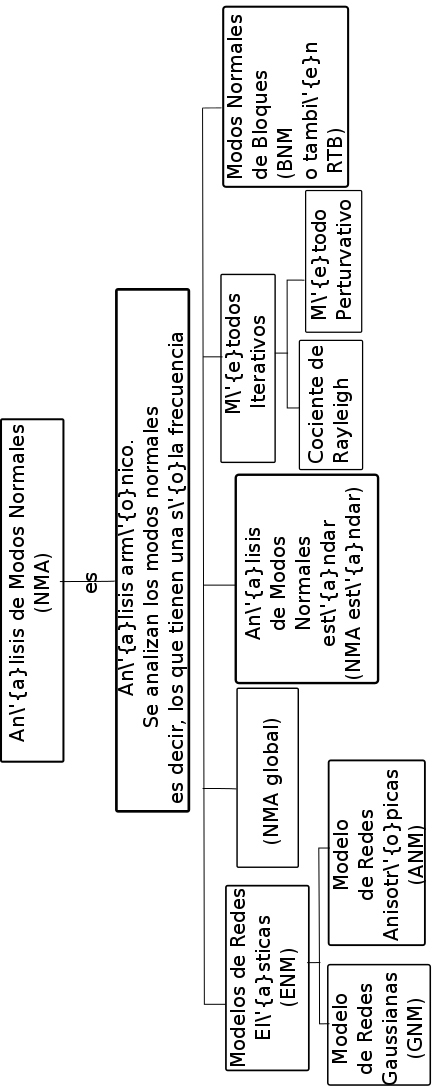
\includegraphics[scale=0.4]{Kap2/mapa.png}%
\caption{Mapa conceptual en el que se dividen los movimientos locales de los movimientos globales, mostrando los tipos de movimientos globales utilizados} \label{fig:movs}
\end{figure}